\newif\ifjp
\newif\ifinternal

\internalfalse

% テキストテンプレート
\ifjp%>>>>>>>>>>>>>>>>>>>>>>>>>>>>>>>>>>>>>>>>>>>>>>>>>>>>>>>>>>>>>>>>>>>
\else%%%%%%%%%%%%%%%%%%%%%%%%%%%%%%%%%%%%%%%%%%%%%%%%%%%%%%%%%%%%%%%%%%%%
\fi%%%%<<<<<<<<<<<<<<<<<<<<<<<<<<<<<<<<<<<<<<<<<<<<<<<<<<<<<<<<<<<<<<<<<<



%% 日本語 以下を有効化
\jptrue
% #!platex manualAll2; dvipdfmx  -o manualAll2jp.pdf manualAll2
%#!platex manualAll2; latexml --noparse --destination=./manual.xml manualAll2.tex; latexmlpost --format=xhtml --destination=./docs/3.4.0/ja/manual.xhtml --split  --novalidate manual.xml

% #!platex manualAll2; latexml --noparse --destination=./manual.xml manualAll2.tex; latexmlpost --format=xhtml --destination=/home/ohori/WWW/JasperWWW/pllab/public_html/smlsharp/docs/3.4.0/ja/manual.xhtml --split  --novalidate manual.xml

% 英語 以下を有効化
% \jpfalse
% #!platex manualAll2; dvipdfmx -o manualAll2en.pdf manualAll2
% #!platex manualAll2; latexml --noparse --destination=./manual.xml manualAll2.tex; latexmlpost --format=xhtml --destination=./docs/3.4.0/en/manual.xhtml --split  --novalidate manual.xml

% #!platex manualAll2; latexml --noparse --destination=./manual.xml manualAll2.tex; latexmlpost --format=xhtml --destination=/home/ohori/WWW/JasperWWW/pllab/public_html/smlsharp/docs/3.4.0/en/manual.xhtml --split  --novalidate manual.xml

\ifjp
\newcommand{\txt}[2]{#1}
\documentclass{jbook}
\else
\newcommand{\txt}[2]{#2}
\documentclass{book}
\fi


% テキストマクロ
% \txt{日本語}{English}


\usepackage{latexsym}
\usepackage{url}
\usepackage{epsfig}
\textwidth 15.9truecm
\textheight 24.6truecm
\oddsidemargin 0in
\evensidemargin 0in
\topmargin -0.5truein


\newcommand{\authors}
{\txt{大堀\ \ 淳\mbox{\ \ \ \ }上野 雄大
\\
東北大学 電気通信研究所
}
{Atsushi Ohori\mbox{\ \ \ \ }Katsuhiro Ueno
\\
RIEC, Tohoku University
}
}

\renewcommand{\today}{\txt{平成29年8月}{August, 2017}}
\date{\today}
\newcommand{\smlsharp}{SML\#}
\newcommand{\version}{3.4.0}

\newcommand{\releaseDate}{2017-08-31}

\newcommand{\seeJapanese}{The English version of this document is under
construction. See the official Japanese documents (unfortunately in Japanese).}


\newcommand\eurl[1]{{\edef\eurlTMP{{#1}}\expandafter\url\eurlTMP}}

\newcommand{\documentUrlJa}{\url{http://www.pllab.riec.tohoku.ac.jp/smlsharp/docs/3.4.0/ja/manual.xhtml}}
\newcommand{\documentUrlEn}{\url{http://www.pllab.riec.tohoku.ac.jp/smlsharp/docs/3.4.0/en/manual.xhtml}}
\newcommand{\smlsharpSize}{\txt{30万}{0.3 millions}}

\newcommand{\code}[1]{\mbox{\large\tt #1}}
\newcommand{\func}{\rightarrow}
\newcommand{\module}[2]{\code{#1}(\code{#2})}
\newcommand{\vbar}{\mbox{\ $|$\ }}

\newcommand{\nonterm}[1]{\mbox{$\,\langle$}{\it #1}\mbox{$\rangle\,$}}
\newcommand{\term}[1]{\mbox{{\tt #1}}}
\newcommand{\optional}[1]{\mbox{$($}{\protect #1}\mbox{$)?$}}
\newcommand{\optionalBegin}{\mbox{$($}}
\newcommand{\optionalEnd}{\mbox{$)?$}}

\newcommand{\ass}{\Gamma}

% \newcommand{\myem}{\mbox{\ \ \ \ \  }}
% \newcommand{\myfm}{\mbox{ \ \ \ \ \ }}
% \newcommand{\myem}{\ \ }
% \newcommand{\myfm}{ \ \ }
\newcommand{\myem}{\mbox{\ \ }}
\newcommand{\myfm}{\mbox{ \ \ }}

\newcommand{\sep}{\mbox{\ \ }}
% \newenvironment{program}{\begin{quote}\begin{large}\begin{tt}}%
%                         {\end{tt}\end{large}\end{quote}}
\newenvironment{program}{\begin{quote}\begin{tt}}%
                        {\end{tt}\end{quote}}
\newenvironment{programPlain}{\begin{large}\begin{tt}}%
	                     {\end{tt}\end{large}}
%%% 用語
\newcommand{\base}{基本}
\newcommand{\baseType}{基本型}
\newcommand{\baseExp}{基本式}
\newcommand{\basePat}{基本パターン}
\newcommand{\ground}{基底}
\newcommand{\instance}{}
\newcommand{\groundInstance}{\ground\instance}
%endInput


%%%%%%%%%%%%%% local definitions %%%%%%%%%%%%%%%%
% \newcommand{\structure}[1]{{\tt #1}\txt{ストラクチャ}{structure}}
\newcommand{\structure}[1]{
\section{{\tt #1}}\label{section:reference:#1}
}
% \newcommand{\signature}[1]{{\tt #1}\txt{シグネチャ}{signature}}
\newcommand{\signature}[2]{
\section{{\tt #1}}\label{section:reference:#2}
}
\newcommand{\br}{\\}
\newcommand{\DECL}[2]{
 \medskip\noindent
 {\tt #1\begin{tabular}[t]{@{}l@{}l}#2\end{tabular}\par}
}
\newcommand{\sigref}[1]{\ref{section:reference:#1}}
\newcommand{\sigitem}[3]
{
& \code{#1}
& \code{#3}
& (\sigref{#2})
\\
}
\newcommand{\DATATYPE}[2]{
 \medskip\noindent
  {\tt\newcommand{\OR}{\\|~&}%
      \newcommand{\Or}{|~}%
      \renewcommand{\br}{\\&}%
  datatype~#1~\begin{tabular}[t]{@{}l@{~}l}=~&#2\end{tabular}\par}
}
\newcommand{\datatype}[2]{
 \medskip\noindent
 {\tt
    \newcommand{\Or}{\vbar}%
    \newcommand{\OR}{\vbar}%
    \renewcommand{\br}{\\}%
    datatype~#1~=~#2
    \par
 }
}
\newcommand{\type}[2]{\DECL{type~#1~=~}{#2}}
\newcommand{\optype}[2]{\DECL{type~#1~(=~}{#2)}}
% \newcommand{\eqtype}[2]{\DECL{eqtype~#1~(=~}{#2)}}
\newcommand{\eqtype}[2]{{eqtype~#1~(=~}{#2)}\par}
\newcommand{\optypeSig}[2]{\DECL{type~#1}{}}
\newcommand{\eqtypeSig}[2]{\DECL{eqtype~#1}{}}
\newcommand{\val}[2]{\code{val~#1~:~#2}\par}
\newcommand{\exception}[1]{\DECL{exception~#1}{}}
\newcommand{\exceptionWithArg}[2]{\DECL{exception~#1~of~}{#2}}
% \renewcommand{\{}{\char`\{}
% \renewcommand{\}}{\char`\}}
% \renewcommand{\_}{\char`\_}
% \renewcommand{\^}{\char`\^}
% \renewcommand{\~}{\char`\~}
\newcommand{\smlsharpspecific}[1]{{\em \smlsharp{}固有\/}: #1}
\newcommand{\Structure}{\subsubsection*{\txt{シグネチャを実装するストラクチャ}{Structures that implement the signature}}}
\newcommand{\Signature}{\subsubsection*{\txt{シグネチャ}{Signature}}}
\newcommand{\Types}{\subsubsection*{\txt{型}{Types}}}
\newcommand{\Interface}{\subsubsection*{\txt{インタフェイス}{Interfce}}}
\newcommand{\Exceptions}{\subsubsection*{\txt{例外}{Exception}}}
\newcommand{\Constants}{\subsubsection*{\txt{定数}{Constants}}}
\newcommand{\Functions}{\subsubsection*{\txt{関数}{Functions}}}
\newcommand{\NestedStructures}{\subsubsection*{\txt{ネストしたストラクチャ}{Nested structures}}}
\newcommand{\NestedSignature}{\subsubsection*{\txt{ネストしたシグネチャ}{Nested signatures}}}
\newcommand{\substructure}[1]{{structure~#1~=~}{$\cdots$}}
\newcommand{\subsignature}[1]{{signature~#1}}
%%%%%%%%%%%%%% local definitions %%%%%%%%%%%%%%%%

\newcommand{\libitem}[2]
{
& \code{#1}
& \code{#2} (\sigref{#2})
\\
}
\newcommand{\stritem}[1]
{
&
& \code{#1} (\sigref{#1})
\\
}



\title{\txt{プログラミング言語\smlsharp{}解説}{\smlsharp{} Document}}
\author{
\authors
}



\begin{document}
\pagenumbering{roman}
\maketitle
 
\tableofcontents

\ifjp%>>>>>>>>>>>>>>>>>>>>>>>>>>>>>>>>>>>>>>>>>>>>>>>>>>>>>>>>>>>>>>>>>>>
{\bf FireFox}などのMathMLを表示可能なブラウザでご覧ください.
\else%%%%%%%%%%%%%%%%%%%%%%%%%%%%%%%%%%%%%%%%%%%%%%%%%%%%%%%%%%%%%%%%%%%%
This document is best viewed with a MathML-capable browser such as {\bf FireFox}.
\fi%%%%<<<<<<<<<<<<<<<<<<<<<<<<<<<<<<<<<<<<<<<<<<<<<<<<<<<<<<<<<<<<<<<<<<

\setcounter{page}{1}
\pagenumbering{arabic}

\part{\txt{概要}{Overview}}
\label{part:outline}

\chapter{\txt{はじめに}{Preface}}

\ifjp%>>>>>>>>>>>>>>>>>>>>>>>>>>>>>>>>>>>>>>>>>>>>>>>>>>>>>>>>>>>>>>>>>>>
	本書は東北大学電気通信研究所で開発された関数型プログラミング言語
\smlsharp{}の公式ドキュメントです.
	\smlsharp{}の概要,
チュートリアル,
\smlsharp{}言語とライブラリの参照マニュアル,
ツールの情報,
さらに,
\smlsharp{}の内部構造に関する詳細な記述,
等を含む総合ドキュメントを意図しています.

	関数型言語に慣れた人はもちろん,これからプログラミングを始めようと
する人にも,\smlsharp{}言語を使って高度なプログラミングを書き始めるために
十分な情報を提供します.
	特に,第\ref{part:tutorial}部のチュートリアルは,関数型言語の基
本的な考え方やMLプログラミングの基礎を含んでおり,ML言語の手軽な教科書と
しても使用できます.
  
	\smlsharp{}は,これら教科書で書かれたStandard MLと後方互換性のあ
る言語です.
	ネイティブコードコンパイラですが,対話型プログラミングもサポート
しており,だれでも手軽にMLプログラミングを楽しむことができます.
	さらに,\smlsharp{}が実現しているC言語とのシームレスな連携などの
機能は,高度で信頼性の要求される本格的な実用的システムの開発にも威力を
発揮すると信じています. 
  
	本ドキュメントを参考に,\smlsharp{}プログラミングをお楽しみくだ
さい. 
	不明な点や要望等は著者にご連絡ください.

\else%%%%%%%%%%%%%%%%%%%%%%%%%%%%%%%%%%%%%%%%%%%%%%%%%%%%%%%%%%%%%%%%%%%%
	This is the official document of \smlsharp{}, a programming
language being developed at Research Institute of Electrical
Communication, Tohoku University.
	This document intends to provide comprehensive information on
\smlsharp{}, including:
tutorials on \smlsharp{} programming, 
reference manuals of the \smlsharp{} language and the basis library,
and,
detailed descriptions of the internals and data structures of the
\smlsharp{} system.

	Send comments and questions to the authors.
\fi%%%%<<<<<<<<<<<<<<<<<<<<<<<<<<<<<<<<<<<<<<<<<<<<<<<<<<<<<<<<<<<<<<<<<<

\begin{flushright}
\txt{
2017年6月\\
\authors
}
{
June, 2017\\
\authors
}
\end{flushright}

\chapter{\txt{本書の構成と執筆状況}{About This Document}}

\ifjp%>>>>>>>>>>>>>>>>>>>>>>>>>>>>>>>>>>>>>>>>>>>>>>>>>>>>>>>>>>>>>>>>>>>
	本書は以下の部から成ります.
\begin{enumerate}
\item
	第\ref{part:outline}部: \smlsharp{}の概要.
\item
	第\ref{part:tutorial}部:\smlsharp{}のチュートリアル.
	\smlsharp{}のインストール方法,
\smlsharp{}の初歩的な使い方,
および
\smlsharp{}の拡張機能の概要を,例と共に説明しています.
	また,関数型言語初学者に向けた,
MLプログラミングのための環境のセットアップ方法や,
Standard MLの基本機能を用いたMLプログラミングの基本も,
本章に含まれています.
	初心者から上級者までを含む全ての\smlsharp{}ユーザーにとって,
この部の内容は有益なはずです.
	先頭から順に一気にお読みになることをおすすめします.
	お急ぎの方は,以下のページにお探しの情報があるかもしれません.
\begin{itemize}
\item {\bf インストール方法:}
第\ref{sec:tutorialInstall}節.
\item {\bf {\tt smlsharp}コマンドの起動モードと起動パラメタ:}
第\ref{sec:tutorialSmlsharpParameter}節.
\item {\bf \smlsharp{}開発チームと連絡先情報:} 
第\ref{sec:smlsharpTeam}節.
\item {\bf \smlsharp{}の名前について:}
第\ref{sec:smlsharpHistory}節.
\item {\bf \smlsharp{}ホームページ:}
\url{http://www.pllab.riec.tohoku.ac.jp/smlsharp/ja/}
\item {\bf \smlsharp{} Document in English:}
\url{http://www.pllab.riec.tohoku.ac.jp/smlsharp/docs/\version/en/manual.xhtml}
\documentUrlEn
\end{itemize}   

\item
	第\ref{part:referenceManual}部:
\smlsharp{}言語およびライブラリの参照マニュアル.

\smlsharp{}言語の構文と意味の定義,および,\smlsharp{}プログラミングに使
用するStandard ML基本ライブラリと\smlsharp{}の機能を活用する種々のライブ
ラリのAPIと機能の定義を含みます.

\item
	第\ref{part:tools}部:
\smlsharp{}付属のツール群({\tt smllex}, {\tt smlyacc}, {\tt smlformat}など)
の解説と参照マニュアル.

\item
	第\ref{part:internals}部:\smlsharp{}コンパイラの内部構造.
\smlsharp{}コンパイラの開発や関数型言語のコンパイラの構築方法に興味の
ある方を対象に,ソースコードとデータ構造の詳細を記述します.

\item
	第\ref{part:bib}部: 参考文献のリスト.
\end{enumerate}

本書に関して,以下の点をご了承ください.
\begin{itemize}
\item 随時頻繁に修正を行います.
	そのため,本文書の配布は当面xhtml形式のみとします.
	近い将来,より完成した版のPDFでの配布を検討中です.

\item この文書は,LaTeXとLaTeXMLを用いて作成しています.
FirefoxなどのMathMLのレンダリングが可能なブラウザでご覧ください.

\item LaTeXMLは日本語化がなされていないようです.
	本文書は{\tt jbook}クラスで書いていますが,LateXMLのpackageに
jbook用が用意されていないため,{\tt book.cls.ltxml}を
{\tt jbook.cls.ltxml}にコピーし使用しています.
	(LateXMLの日本語クラスパッケージをご存知の方はお教えください.)
\end{itemize}

\else%%%%%%%%%%%%%%%%%%%%%%%%%%%%%%%%%%%%%%%%%%%%%%%%%%%%%%%%%%%%%%%%%%%%
	This documents consist of the following parts.
\begin{enumerate}
\item
	Part~\ref{part:outline}:
an overview of the \smlsharp{}.
\item
	Part~\ref{part:tutorial}: \smlsharp{} tutorials.
	The tutorials are structured in such a way that the reader can
learn \smlsharp{} from programming basics to advanced programming
features provided by \smlsharp{}.
	We recommend to read through this part quickly.

	If you are in a harry, you may find the desired information in
one of the following pages.
\begin{itemize}
\item {\bf How to install \smlsharp{}}:
Section \ref{sec:tutorialInstall}.
\item {\bf {\tt smlsharp} command parameters}:
Section \ref{sec:tutorialSmlsharpParameter}.
\item {\bf \smlsharp{} development team and contact information}:
Section \ref{sec:smlsharpTeam}.
\item {\bf On the name of \smlsharp{}}:
Section \ref{sec:smlsharpHistory} (History of \smlsharp).
\item {\bf \smlsharp{} web page}: 
\url{http://www.pllab.riec.tohoku.ac.jp/smlsharp/}
\item {\bf \smlsharp{} document in Japanese}:
\url{http://www.pllab.riec.tohoku.ac.jp/smlsharp/docs/\version/ja/manual.xhtml}
\documentUrlJa
\end{itemize}

\item
	Part~\ref{part:referenceManual}:
reference manuals on the \smlsharp{} language and the libraries
including Standard ML Basis Library.

\item
	Part~\ref{part:tools}:
Reference manuals on \smlsharp{} tools 
({\tt smllex}, {\tt smlyacc}, {\tt smlformat} etc).

\item
	Part~\ref{part:internals}:
	The internals and data structures of the \smlsharp{} system.

\item
	Part~\ref{part:bib}: references.
\end{enumerate}

In reading this document, please note the following.
\begin{itemize}
\item 
	This document is frequently revised and updated.
	For this reason, the currently version is distributed only on
this web server.
	In near future, we plan to include a more complete version of
this document (both in PDF and XHTML format) in the \smlsharp{}
distribution.

\item 
	This document is written in LaTeX and processed with LaTeXML.
	It is best viewed with a MathML-capable browser such as {\bf
Firefox}.
\end{itemize}
\fi%%%%<<<<<<<<<<<<<<<<<<<<<<<<<<<<<<<<<<<<<<<<<<<<<<<<<<<<<<<<<<<<<<<<<<


\chapter{\txt{\smlsharp{}の概要}{Overview of \smlsharp{}}}
\label{chap:intro}
\ifjp%>>>>>>>>>>>>>>>>>>>>>>>>>>>>>>>>>>>>>>>>>>>>>>>>>>>>>>>>>>>>>>>>>>>
本章では\smlsharp{}言語の概要を説明します.
\else%%%%%%%%%%%%%%%%%%%%%%%%%%%%%%%%%%%%%%%%%%%%%%%%%%%%%%%%%%%%%%%%%%%%
This chapter outlines the \smlsharp{} language and the compiler.
\fi%%%%<<<<<<<<<<<<<<<<<<<<<<<<<<<<<<<<<<<<<<<<<<<<<<<<<<<<<<<<<<<<<<<<<<

\section{\txt{\smlsharp{}とは?}{What is \smlsharp{}?}}
\label{sec:whatIsSmlsharp}
\ifjp%>>>>>>>>>>>>>>>>>>>>>>>>>>>>>>>>>>>>>>>>>>>>>>>>>>>>>>>>>>>>>>>>>>>
	\smlsharp{}は,以下のような特徴をもったML系関数型プログラミング
言語です.
\begin{enumerate}
\item {\bf Standard MLとの後方互換性.}
	\smlsharp{}は,ML系言語の標準の厳密な仕様であるStandard MLとの
後方互換性を持っています.
	Standard MLの形式的な仕様\cite{sml}を満たすすべての
プログラムをコンパイルできます.

\item {\bf レコード多相性.}
	レコード多相性\cite{ohor95toplas}は,オブジェクトやデータベース
のタプルなどに現れるラベル付きレコードをML言語に完全に統合するために必要
な型システムの機能です.
	\smlsharp{}は,この機能を完全にサポートしています.

\item {\bf SQLのシームレスな統合.}
	SQLはデータベースの標準問い合わせ言語であり,データベースを利用
するプログラムで必ず必要となる機能です.
	\smlsharp{}は,SQLの一部の機能をライブラリとして提供するのでは
なく,SQLクエリそのものを多相型をもつ第一級の式として統合しています.
	この機能により,複雑なプログラムデータベース操作を,MLプログラム
の中で直接プログラムすることができます.
	
\item {\bf C言語との直接連携.}
	システムプログラミングを含む種々のOSの機能の利用にはC言語で記述
されたライブラリへのアクセスが必要となります.
	\smlsharp{}では,名前を外部名宣言するだけで,C言語で書かれCコン
パイラでコンパイルされた関数を呼び出すことができます.

\item {\bf マルチコアCPU上のネイティブスレッドのサポート.}
	\smlsharp{}の並行かつオブジェクトを動かさないGCの機能により,
C言語との連携機能を使い,OSのスレッドライブラリを直接呼び出すことができ
ます.
	従って,OSがマルチコアCPU上での並列実行をサポートしさえすれば,
スレッドを使った高水準なMLプログラムを書き,マルチコアCPU上で効率良く
実行することができます.

\item {\bf 分割コンパイルとリンク.}
	\smlsharp{}は,従来のインクリメンタルなコンパイルではない,真の分
割コンパイルを実現しています.
	各モジュールのインターフェイスの確定後は,各モジュールを独立に開
発しコンパイルやテストできます.
	さらに,\smlsharp{}コンパイラは,分割コンパイルの対象となる各ソー
スコードを,システム標準のオブジェクトファイル(例えばLinuxならば
ELFフォーマット)にコンパイルし,システムのリンカーでCのライブラリなどと
ともにリンクします.
	この機能により,Standard MLだけでなくC言語やSQLなどをも使う
大規模プログラムを安全かつ効率的に開発することができます.
\end{enumerate}

	\smlsharp{}コンパイラおよび実行時処理系は,東北大学電気通信研究
所大堀研究室で開発され,東北大学が著作権保有するオープンソースソフトウェ
アです.
	BSDスタイルの\smlsharp{}ライセンス(\ref{sec:smlsharpLicence}節参照)に
よって公開されており,だれでも自由に利用することができます.
	このライセンスは,二次著作物(つまりコンパイラで作成されたシステ
ムなど)に関する制限の少ないフリーソフトウェアライセンスであり,企業の商
品開発にも安心して使用できます.

\else%%%%%%%%%%%%%%%%%%%%%%%%%%%%%%%%%%%%%%%%%%%%%%%%%%%%%%%%%%%%%%%%%%%%

	\smlsharp{} is a new programming language in the ML-family,
having the following features.
\begin{enumerate}
\item {\bf Downward compatibility with Standard ML.}
	\smlsharp{} can compile all programs that conform to the
definition of the Standard ML\cite{sml}.

\item {\bf Record polymorphism.}
	\smlsharp{} supports record polymorphism \cite{ohor95toplas}.
	In \smlsharp{} , field selection operators {\bf\tt \#\nonterm{label}}
and record patterns {\bf\tt \{\nonterm{field-pat},...\}} are fully
polymorphic.
	This feature is essential in modular development of programs
manipulating records, and is the key to extend ML with SQL.

\item {\bf Seamless integration of SQL.}
	\smlsharp{} seamlessly integrates (currently a subset of) SQL.
	Instead of providing built-in primitives to access
database servers, \smlsharp{} integrate SQL expressions themselves as
polymorphically-typed first-class citizens.
	This allows the programmer to directly access databases in
your polymorphic ML code.

\item {\bf Direct interface to C.}
	\smlsharp{} programs can directly call C functions of your own
coding or in system libraries.
	The programmer need only declare their names and types, without
writing mysterious ``stubs'' or conversion functions. 
	The \smlsharp{} generates external references to C functions,
which are resolved and linked by the system linker.
	Both static and dynamic linking are supported.

\item {\bf Separate compilation and linking.}
	\smlsharp{} supports true separate compilation and linking.
	By writing an interface file, each source file is compiled
separately into an object file in the standard system format (e.g.\ ELF
format.)
	The separately compiled object files are then linked together
possibly with C functions and libraries into an executable program.

\item {\bf Multithread support for multicore CPUs.}
	The non-moving GC \cite{ueno11icfp} and direct C interface allow
\smlsharp{} code to directly call POSIX thread library.
	As far as the OS thread library support a multicore CPU,
\smlsharp{} program automatically obtains multithread capability for
multicore CPUs.
	With the non-moving fully concurrent GC we have just developed, 
concurrent threads run efficiently on a multicore CPU.

\end{enumerate}

	The \smlsharp{} compiler and its runtime system are developed at
Research Institute of Electrical Communication,  Tohoku University.
	They are open-source software distributed with a BSD-style
\smlsharp{} license (\ref{sec:smlsharpLicence}).
\fi%%%%<<<<<<<<<<<<<<<<<<<<<<<<<<<<<<<<<<<<<<<<<<<<<<<<<<<<<<<<<<<<<<<<<<

\section{\txt{\smlsharp{}の歴史}{History of \smlsharp{}}}
\label{sec:smlsharpHistory}

\ifjp%>>>>>>>>>>>>>>>>>>>>>>>>>>>>>>>>>>>>>>>>>>>>>>>>>>>>>>>>>>>>>>>>>>>
	\smlsharp{}の起源は,大堀等によるデータベースコミュニティへの
Machiavelli言語の提案\cite{ohor89sigmod}に遡ることができます.
	この論文では,レコード多相を含むMLはSQLを包摂できることが示され,
その有用性がプロトタイプの実装によってしめされています.

	その後,1993年,沖電気工業(株)関西総合研究所にて,大堀により,
Standard ML of New Jerseyコンパイラに多相型レコード演算を加え拡張したプ
ロトタイプ{\bf SML\# of Kansai}が開発されました.
	その時の\smlsharp{}のtypesメーリングリストへのアナウンスは,今で
もインターネット上に記録されています
(
\url{http://www.funet.fi/pub/languages/ml/sml%23/description}
).

	{\bf SML\# of Kansai}の名前は,このコンパイラにて初めて多相型が与えら
れたレコード演算子"{\bf \code{\#}}"を象徴するものです.
	このコンパイラは,1996年ACM TOPLASに出版されたコード多相性に関する論文
\cite{ohor95toplas}で,{\bf \smlsharp{}}の名前で紹介されています.

	その後,より完全な\smlsharp{}コンパイラの開発の努力が継続されま
した.

	2003年に,北陸先端科学技術大学院大学にて,文部科学省リーディング
プロジェクトe-Society基盤ソフトウェアの総合開発「高い生産性をもつ高信頼
ソフトウエア作成技術の開発」
(領域代表者:片山卓也)
の一つの課題
「プログラムの自動解析に基づく高信頼ソフトウェアシステム構築技術」(2003年―2008年,究代表者:大堀 淳)
(
\url{http://www.tkl.iis.u-tokyo.ac.jp/e-society/index.html}
)
として,
次世代ML系関数型言語\smlsharp{}をスクラッチから開発するプロジェクトを開始しました.

2006年4月,プロジェクトは,大堀とともに東北大学電気通信研究所に移り開発
を継続しています.

2008年のe-Societyプロジェクト終了後も,東北大学電気通信研究所大堀研究室
にて,\smlsharp{}の研究開発を続けています.

\else%%%%%%%%%%%%%%%%%%%%%%%%%%%%%%%%%%%%%%%%%%%%%%%%%%%%%%%%%%%%%%%%%%%%
	The origin of the \smlsharp{} can be traced back to the proposal
of Machiavelli published in \cite{ohor89sigmod}.
	This paper showed that ML with record polymorphism can be
extended with SQL and reported a implementation of a prototype interpreter. 

	In 1993, Atsushi Ohori extended the Standard ML of New Jersey
compiler at Kansai Laboratory of Oki Electric, and named the
experimental prototype {\bf SML\# of Kansai}.
	The Internet still remembers the posting of {\bf SML\# of
Kansai} to the types mailing list  
(\url{http://www.funet.fi/pub/languages/ml/sml%23/description}).

	The name {\bf SML\# of Kansai} symbolized the field selector {\bf\tt
\#\nonterm{label}}, which was given a polymorphic type for the first
time by this compiler.
	This compiler was reported in the ACM TOPLAS article on record
polymorphism \cite{ohor95toplas} as {\bf \smlsharp{}}.

	To support not only record polymorphism but also
inseparability and other practically important features, we decided 
to develop a new SML-style language from scratch, and in 2003, we
started the \smlsharp{} compiler project at Japan Advanced Institute of 
Science and Technology as a part of the e-Society project 
(
\url{http://www.tkl.iis.u-tokyo.ac.jp/e-society/index.html}
)
funded by the Japan ministry of science, education and technologies

	In 2006, the project moved to Tohoku University.
\fi%%%%<<<<<<<<<<<<<<<<<<<<<<<<<<<<<<<<<<<<<<<<<<<<<<<<<<<<<<<<<<<<<<<<<<

\section{
\txt{\smlsharp{}開発チームと連絡先情報}
{\smlsharp{} Development Team and Contact Information}
}
\label{sec:smlsharpTeam}

\ifjp%>>>>>>>>>>>>>>>>>>>>>>>>>>>>>>>>>>>>>>>>>>>>>>>>>>>>>>>>>>>>>>>>>>>
	現在(\releaseDate)\smlsharp{}は,
\begin{itemize}
\item 
大堀 淳(東北大学電気通信研究所)
\item 
上野雄大(東北大学電気通信研究所)
\end{itemize}
の2名が,大学院大学院情報科学研究科の大堀研究室に所属の大学院生の協力の
下,開発を行なっています.

	\smlsharp{}のこれまでの主な開発者は以下の通りです.
	(敬称は略させていただいています.
	所属は\smlsharp{}の開発に携わった時のものです.)
\begin{itemize}
\item 大堀 淳(北陸先端科学技術大学院大学情報科学研究科,東北大学電気通信研究所)
\item 大和谷 潔(算譜工房)
\item Nguyen Huu Duc(北陸先端科学技術大学院大学情報科学研究科,東北大学電気通信研究所)
\item Liu Bochao(北陸先端科学技術大学院大学情報科学研究科,東北大学電気通信研究所)
\item 纓坂 智(北陸先端科学技術大学院大学情報科学研究科)
\item 上野雄大(北陸先端科学技術大学院大学情報科学研究科,東北大学電気通信研究所)
\end{itemize}

	東北大学電気通信研究所では,\smlsharp{}に関する情報共有の目的で
以下のwebサイトやメーリングリストを管理しています.
\begin{itemize}
\item \smlsharp{}ホームページ.
\url{http://www.pllab.riec.tohoku.ac.jp/smlsharp/ja/}
コンパイラや本書を含む文書の最新版などもここからダウンロードできます.

\item Twitterアカウント {\tt @smlsharp}.
\smlsharp{}に関する最新情報をツイートします.

	修正・執筆にあたっては,twitterなどでの\smlsharp{}や本書へのコメ
ントなども,本書の改善の参考にさせて頂いております.
	個々に言及いたしませんが,本書をご覧頂きコメントをお寄せ頂いた
方々に感謝いたします. 

\item \smlsharp{}開発者への連絡メールアドレス
{\tt smlsharp-dev@ml.riec.tohoku.ac.jp}.
%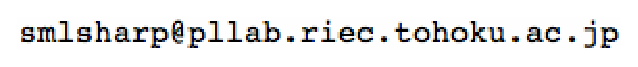
\epsfig{file=smlsharp-list.eps,width=0.4\textwidth}
各種問い合わせや共同研究の提案などにご利用ください.

\end{itemize}
\else%%%%%%%%%%%%%%%%%%%%%%%%%%%%%%%%%%%%%%%%%%%%%%%%%%%%%%%%%%%%%%%%%%%%
	At present (\releaseDate), \smlsharp{} is being developed by
\begin{itemize}
\item 
Atsushi Ohori(RIEC, Tohoku University)
\item 
Katsuhiro Ueno (RIEC, Tohoku University)
\end{itemize}
with help of graduate students.

	The past \smlsharp{} development team members include (with the
affiliation at the time of development):
\begin{itemize}
\item Atsushi Ohori (School of Information Science, JAIST; RIEC, Tohoku University)
\item Kiyoshi Yamatodani (Sanpukoubou Inc)
\item Nguyen Huu Duc (School of Information Science, JAIST; RIEC, Tohoku University)
\item Liu Bochao (School of Information Science, JAIST; RIEC, Tohoku University)
\item Satoshi Osaka (School of Information Science, JAIST)
\item Katsuhiro Ueno (School of Information Science, JAIST; RIEC, Tohoku University)
\end{itemize}

	Contact information regarding \smlsharp{}:
\begin{itemize}
\item \smlsharp{} home page:
\url{http://www.pllab.riec.tohoku.ac.jp/smlsharp/ja/}

%\item \smlsharp{} mailing list:
%{\tt smlsharp-list@pllab.riec.tohoku.ac.jp}
%
%	This list is for general discussion on \smlsharp{}.
%	We use Japanese and English in discussion.
%	To post a message, you need to subscribe to this list.
%	All the messages are made available on the Web.

%%%%%%%%%%%%%%%%%%ToDo: 参加方法
%How to subscribe:\url{http://www.pllab.riec.tohoku.ac.jp/mailman/listinfo.cgi/smlsharp-list?language=ja}\\
%Mail archive:\url{http://www.pllab.riec.tohoku.ac.jp/pipermail/smlsharp-list/}

\item \smlsharp{} twitter account:
{\tt @smlsharp}

	We tweet the latest information about \smlsharp{} on this account.
	
\item Email address of the \smlsharp{} development team :
{\tt smlsharp-dev@ml.riec.tohoku.ac.jp}
%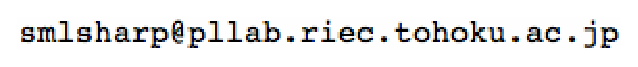
\epsfig{file=smlsharp-list.eps,width=0.4\textwidth}

Send your questions, requests, and comments to the development team.
\end{itemize}
\fi%%%%<<<<<<<<<<<<<<<<<<<<<<<<<<<<<<<<<<<<<<<<<<<<<<<<<<<<<<<<<<<<<<<<<<

\section{\txt{謝辞}{Acknowledgments}}
\label{sec:acknowledgements}
	
\ifjp%>>>>>>>>>>>>>>>>>>>>>>>>>>>>>>>>>>>>>>>>>>>>>>>>>>>>>>>>>>>>>>>>>>>
	2003年にスタートした\smlsharp{}開発の過程では,以下を含む色々な
ご指導やご協力を頂きました.
	ここに謝意を表します.
\else%%%%%%%%%%%%%%%%%%%%%%%%%%%%%%%%%%%%%%%%%%%%%%%%%%%%%%%%%%%%%%%%%%%%
	From its start in 2003, we have benefited from many peoples and
organizations.
\fi%%%%<<<<<<<<<<<<<<<<<<<<<<<<<<<<<<<<<<<<<<<<<<<<<<<<<<<<<<<<<<<<<<<<<<
	
\subsection{\txt{プロジェクトファンディング}{Project funding}}

\ifjp%>>>>>>>>>>>>>>>>>>>>>>>>>>>>>>>>>>>>>>>>>>>>>>>>>>>>>>>>>>>>>>>>>>>
	\smlsharp{}言語の研究開発は,2003年から5年間の文部科学省リーディ
ングプロジェクトe-Society基盤ソフトウェアの総合開発「高い生産性をもつ高
信頼ソフトウェア作成技術の開発」
(\url{http://www.tkl.iis.u-tokyo.ac.jp/e-society/index.html)}
の一つの課題
「プログラムの自動解析に基づく高信頼ソフトウェアシステム構築技術」(究代
表者:大堀 淳)としてスタートをきることができました.
	このプロジェクトの主要な目標が\smlsharp{}言語コンパイラの開発で
した.
	\smlsharp{}は開発ソースの総量が\smlsharpSize{}行を超える大規模シ
ステムです.
	このプロジェクトの支援がなければ,\smlsharp{}の開発は困難であっ
たと思われます.
	文部科学省,e-Societyの領域代表の片山卓也先生,および関係各位に
深謝いたします.
	この大型プロジェクトに加え,\smlsharp{}の理論や実装方式の研究開
発には,複数の科学研究費補助金によるサポートを受けています.

\else%%%%%%%%%%%%%%%%%%%%%%%%%%%%%%%%%%%%%%%%%%%%%%%%%%%%%%%%%%%%%%%%%%%%
	\smlsharp{} development was started as a part of the 5 year
project``e-Society leading project: highly productive reliable software
development technologies (Project Director: Professor Takuya Katayama)'' 
under the title
``
reliable software development technology based on automatic program analysis
(chief investigator: Atsushi Ohori)
''
(\url{http://www.tkl.iis.u-tokyo.ac.jp/e-society/index.html})
sponsored by the Japan ministry of science, education and technologies.

\fi%%%%<<<<<<<<<<<<<<<<<<<<<<<<<<<<<<<<<<<<<<<<<<<<<<<<<<<<<<<<<<<<<<<<<<

\subsection{
\txt{\smlsharp{}が使用しているソフトウエア}
    {Third-party code and software tool used in \smlsharp{} development}
}

\ifjp%>>>>>>>>>>>>>>>>>>>>>>>>>>>>>>>>>>>>>>>>>>>>>>>>>>>>>>>>>>>>>>>>>>>
	\smlsharp{}言語は,第1.0版以降は,\smlsharp{}自身でコンパ
イルし開発を行なっていますが,それ以前は,Standard ML of New Jerseyおよ
びMLtonのStandard MLコンパイラを使って開発を行いました.

	\smlsharp{}は前節(\ref{sec:smlsharpTeam})の開発チー
ムによって開発されたソフトウェアです.
	ソースコードの殆どをスクラッチから開発しましたが,一部に以下のコー
ドを利用しています.

\begin{center}
\begin{tabular}{|l|l|l|}
\hline
内容 & \smlsharp{}ソース上の位置 & ソース
\\\hline
ML-Yacc & src/ml-yacc  & Standard ML of New Jersey 110.73
\\\hline
ML-Lex & src/ml-lex  & Standard ML of New Jersey 110.73
\\\hline
SML/NJ Library & src/smlnj-lib &  Standard ML of New Jersey 110.73
\\\hline
TextIO,
BinIO,
OS,
Date,
Timer
&
src/smlnj
&
Standard ML of New Jersey 110.73
\\\hline
浮動小数点/
文字列変換関数
&
src/runtime/netlib
&
the Netlib
\\\hline
SMLFormatの
SML文法定義
&
src/smlformat/generator/main/
&
Standard ML of New Jersey 110.73
\\\hline
\end{tabular}
\end{center}

	これらソースは,いずれも\smlsharp{}ライセンスと整合性あるライセ
ンスで配布されているオープンソースソフトウェアです.
	「\smlsharp{}ソース上の位置」およびソースパッケージのトップレベル
にそれぞれのライセンスが添付されています.
\else%%%%%%%%%%%%%%%%%%%%%%%%%%%%%%%%%%%%%%%%%%%%%%%%%%%%%%%%%%%%%%%%%%%%

	Since the version 1.0 had completed, \smlsharp{} has been
developed by the \smlsharp{} compiler itself.
	Before that, we had used Standard ML of New Jersey for
development and MLTon compiler for building distributions.  

	The \smlsharp{} compiler is a software developed by the
\smlsharp{} development team (\ref{sec:smlsharpTeam}).
	We have wrote most of the code of \smlsharp{} compiler from
scratch, except for the following codes:

\begin{center}
\begin{tabular}{|c|c|c|}
\hline
contents & location in \smlsharp{} distribution & source code
\\\hline
ML-Yacc & src/ml-yacc  & Standard ML of New Jersey 110.73
\\\hline
ML-Lex & src/ml-lex  & Standard ML of New Jersey 110.73
\\\hline
SML/NJ Library & src/smlnj-lib &  Standard ML of New Jersey 110.73
\\\hline
{\tt TextIO},
{\tt BinIO},
{\tt OS},
{\tt Date},
{\tt Timer}
structures
&
src/smlnj
&
Standard ML of New Jersey 110.73
\\\hline
floating point-string conversion
(dtoa.c)
&
src/runtime/netlib
&
the Netlib
\\\hline
SML grammar definition used 
in SMLFormat tool
&
src/smlformat/generator/main/
&
Standard ML of New Jersey 110.73
\\\hline
\end{tabular}
\end{center}

	All of the above are open-source software that are compatible
with \smlsharp{} license.
	The \smlsharp{} source distribution includes the license of each
of them at the ``location in \smlsharp{} distribution'' show above.
\fi%%%%<<<<<<<<<<<<<<<<<<<<<<<<<<<<<<<<<<<<<<<<<<<<<<<<<<<<<<<<<<<<<<<<<<

\subsection{\txt{研究開発協力者}{Collaborators}}

\ifjp%>>>>>>>>>>>>>>>>>>>>>>>>>>>>>>>>>>>>>>>>>>>>>>>>>>>>>>>>>>>>>>>>>>>
	\smlsharp{}言語の開発にあたっては,多くの人々からの指導を受けま
した.
	過去現在の開発チーム(第(\ref{sec:smlsharpTeam})節)以外で特に
貢献のあった方々は以下の通りです.
\begin{itemize}
\item 篠埜功氏.
	大堀と共に,関数フュージョン機能を持つ新たしいインラインの理論お
よびその実験的な実装を行いました.
	この機能は実験的な実装がありますが,まだ十分な完成度が得られてお
らず\smlsharp{}\version{}版に組み込まれていませんが,将来取り入れたいと
考えています.
\item 大友聡顕氏.
	大堀,上野と共に,オブジェクトを動かさないGCの研究開発に携わり,
初期の実験的な実装を行い,この方式が有望であることを確認しました.
	この成果は,現在のオブジェクトを動かさないGCの方式の開発と実装の
契機となったものです.
\end{itemize}
	これらの方々以外にも,\smlsharp{}は,大堀等との共同で行なった様々
な型理論やコンパイル方式の基礎研究を基に設計されています.
	現在の\smlsharp{}言語に直接生かされている出版された基礎研究成果
には以下のものが含まれます.
\begin{itemize}
\item レコード多相性の理論\cite{ohor92popl,ohor95toplas}.
\item データベースの型推論\cite{ohor88lfp}.
\item データベース言語(Machiavelli)\cite{ohor89sigmod,bune96tods}.
\item ランク1多相性の型理論\cite{ohor99icfp}.
\item MLのunboxed意味論\cite{ohor97unbox}.
\item MLにおける自然なデータ表現\cite{nguyen06ppdp}.
\item 軽量の関数融合\cite{ohor07popl}.
\item オブジェクトを動かさないGC\cite{ueno11icfp}.
\item SQLの統合方式\cite{ohori11icfp}.
\item JSONサポート\cite{ohori16ecoop}.
\item 並行GC\cite{ueno16icfp}.
\end{itemize}
	それ以外にも多くの共同研究者から色々な機会に示唆や助言を頂いてお
り,それらは1989年にまで遡りますが,それらの方々の列挙は割愛させてい
ただきます.
\else%%%%%%%%%%%%%%%%%%%%%%%%%%%%%%%%%%%%%%%%%%%%%%%%%%%%%%%%%%%%%%%%%%%%

	Many people have contributed to research and development of
\smlsharp{}.
	In addition to the development team (Section
\ref{sec:smlsharpTeam}), the following people directly contributed to 
\smlsharp{} research.
\begin{itemize}
\item Isao Sasano.
With Atsushi Ohori, he investigated 
``Lightweight fusion by fixed point promotion'' and 
developed an experimental inlining module that performs lightweight
fusion.
	This feature is experimental and has not yet been integrated in
\smlsharp{} compiler, but we plan to adopt this method in a future
version.
\item Toshihiko Otomo.
	With Atsushi Ohori and Katsuhiro Ueno, he investigated the
possibility of non-moving collector and showed an initial experimental
result indicating that a non-moving GC is viable in functional
languages.
\end{itemize}
	Many other people helped us through collaborative research with
Atsushi Ohori and others to develop type-theory and compilation methods
that underlie \smlsharp{} compiler.
	\smlsharp{} compiler is directly based on the
following research results, some of them were collaboratively done.
\begin{itemize}
\item record polymorphism \cite{ohor92popl,ohor95toplas}.
\item database type inference \cite{ohor88lfp}.
\item database language (Machiavelli)\cite{ohor89sigmod,bune96tods}.
\item rank-1 polymorphism \cite{ohor99icfp}.
\item unboxed semantics of ML \cite{ohor97unbox}.
\item natural data representation for ML \cite{nguyen06ppdp}.
\item lightweight fusion \cite{ohor07popl}.
\item efficient non-moving GC\cite{ueno11icfp}.
\item implementation method for SQL integration\cite{ohori11icfp}.
\item JSON support\cite{ohori16ecoop}.
\item fully concurrent GC\cite{ueno16icfp}.
\end{itemize}
	We have also benefited from many other researchers from 1989.
	We refrain from compiling a comprehensive list, which seems to
be impossible. 
\fi%%%%<<<<<<<<<<<<<<<<<<<<<<<<<<<<<<<<<<<<<<<<<<<<<<<<<<<<<<<<<<<<<<<<<<

\section{
\txt{\smlsharp{}第\version{}版の機能と制限}
{Limitations in \smlsharp{} version \version{}}
}
\label{sec:smlsharpLimitation}

\ifjp%>>>>>>>>>>>>>>>>>>>>>>>>>>>>>>>>>>>>>>>>>>>>>>>>>>>>>>>>>>>>>>>>>>>
	我々開発チームは第\ref{sec:whatIsSmlsharp}節でのべた機能をすべて
開発し\smlsharp{}開発開始時に目標とした機能を実現しています.
	第\version{}版にその殆どが含まれていますが,以下の制約があります.
\begin{enumerate}
\item ターゲットアーキテクチャ.
	現在の\smlsharp{}コンパイラは,Intelアーキテクチャ(x86\_64)向けのコードのみ生成可能です.
	将来,マルチターゲット化を行う予定です.
%\item Windows版の対話型ループの制約.
%	\smlsharp{}\version{}版は,すべて一つのネイティブコードコンパイ
%ラで動いています.
%	対話型ループも,(1)ユーザ入力のコンパイル,
%(2)現在のコンパイラにリンク,
%(3)動的にロード,のサイクルによって実現されています.
%	この中で(2)のリンクをWindowsシステム上で実現するためには,シ
%ステムの制約上,これまでに作られたオブジェクトファイル毎にリンクのための
%ファイルをコマンドラインで指定する必要があります.
%	このファイル数が,対話型環境での入力に従って増えて行きます.
%	そのため,Windows上の対話型環境の連続使用は,コマンドラインの最
%大文字数によって制約されます.

\item 最適化.
	現在のバージョンには,インライニングや定数の伝播などの基本的な最
適化も十分に実装されていません.
	従って,コンパイル時間,コンパイルされたコードの実行時間もともに
十分とは言えません.
	将来の版では,他の最適化コンパイラに比肩する速度が得られると期待
しています.

\item PthreadsとMassiveThreadsの排他的使用.
	現在のバージョンでは,Pthreads(POSIX thread)とMassiveThreadsを
同時に使用することはできません.
	これらの切り替えは,\smlsharp{}コンパイラのビルド時に,
ビルドオプションを指定することにより行います.
	MassiveThreadsを有効にして(これがデフォルトです)ビルドした
\smlsharp{}コンパイラでPthreadsライブラリを使うプログラムをコンパイルすると,
そのプログラムは正常に動かなくなります.

\end{enumerate}
\else%%%%%%%%%%%%%%%%%%%%%%%%%%%%%%%%%%%%%%%%%%%%%%%%%%%%%%%%%%%%%%%%%%%%
	We have successfully developed all the features listed in
Section~\ref{sec:whatIsSmlsharp}, which include all the features that we
had initially aimed at. 
	The version \version{} contains most of them, with the following 
restrictions.
\begin{enumerate}
\item {\bf Target Architecture.}

	The current compiler only generates x86-64 code.

\item {\bf Optimization.}

	In this version, optimization is far from adequate; it does not
even implement standard ones such as inlining and constant propagation.
	So both the compilation time and the speed of generated code are
not very satisfactory.
	We have started design and development of optimizing \smlsharp{}
compiler, and hope that we will provide an optimized \smlsharp{}
compiler that is as fast as other mature compilers.

\item {Exclusive use of Pthreads and MassiveThreads}
	In this version, you cannot make both Pthreads and MassiveThreads
support available at the same time.
	You need to choose one of them at the time of building
\smlsharp{} compiler.
	If you build the \smlsharp{} compiler with enabling MassiveThreads
support (by default) and compile a Pthreads program by that compiler,
the program does not work properly.

\end{enumerate}
\fi%%%%<<<<<<<<<<<<<<<<<<<<<<<<<<<<<<<<<<<<<<<<<<<<<<<<<<<<<<<<<<<<<<<<<<

\chapter{\txt{\smlsharp{}ライセンス}{\smlsharp{} License}}
\label{sec:smlsharpLicence}

Copyright (c) 2006 - 2017, Tohoku University.\\
All rights reserved.\\

Redistribution and use in source and binary forms, with or without
modification, are permitted provided that the following conditions are
met:

\begin{itemize}
\item 
  Redistributions of source code must retain the above copyright
  notice, this list of conditions and the following disclaimer. 
\item 
  Redistributions in binary form must reproduce the above
  copyright notice, this list of conditions and the following disclaimer
  in the documentation and/or other materials provided with the
  distribution. 
\item 
  Neither the name of Tohoku University nor the names of its
  contributors may be used to endorse or promote products derived from
  this software without specific prior written permission.  
\end{itemize}

THIS SOFTWARE IS PROVIDED BY TOHOKU UNIVERSITY AND CONTRIBUTORS "AS IS"
AND ANY EXPRESS OR IMPLIED WARRANTIES, INCLUDING, BUT NOT LIMITED TO,
THE IMPLIED WARRANTIES OF MERCHANTABILITY AND FITNESS FOR A PARTICULAR
PURPOSE ARE DISCLAIMED. IN NO EVENT SHALL TOHOKU UNIVERSITY OR
CONTRIBUTORS BE LIABLE FOR ANY DIRECT, INDIRECT, INCIDENTAL, SPECIAL,
EXEMPLARY, OR CONSEQUENTIAL DAMAGES (INCLUDING, BUT NOT LIMITED TO,
PROCUREMENT OF SUBSTITUTE GOODS OR SERVICES; LOSS OF USE, DATA, OR
PROFITS; OR BUSINESS INTERRUPTION) HOWEVER CAUSED AND ON ANY THEORY OF
LIABILITY, WHETHER IN CONTRACT, STRICT LIABILITY, OR TORT (INCLUDING
NEGLIGENCE OR OTHERWISE) ARISING IN ANY WAY OUT OF THE USE OF THIS
SOFTWARE, EVEN IF ADVISED OF THE POSSIBILITY OF SUCH DAMAGE.

\part{\txt{チュートリアル}{Tutorials}}
\label{part:tutorial}

\chapter{\txt{\smlsharp{}プログラミング環境の準備}
{Setting up \smlsharp{} programming environment}
}
\label{chap:tutorialEnvironment}

\ifjp%>>>>>>>>>>>>>>>>>>>>>>>>>>>>>>>>>>>>>>>>>>>>>>>>>>>>>>>>>>>>>>>>>>>
	第2部では,\smlsharp{}でプログラミングをマスターするための
チュートリアルを提供します.
	まず\smlsharp{}プログラミング環境を整えましょう.
\else%%%%%%%%%%%%%%%%%%%%%%%%%%%%%%%%%%%%%%%%%%%%%%%%%%%%%%%%%%%%%%%%%%%%
	The part~\ref{part:tutorial} provides tutorials to get started
writing \smlsharp{} programs.

	Let us begin by setting up a programming environment.
\fi%%%%<<<<<<<<<<<<<<<<<<<<<<<<<<<<<<<<<<<<<<<<<<<<<<<<<<<<<<<<<<<<<<<<<<

\section{
\txt{Unix系OS,Emacsエディタ,その他ツールの整備}
    {Unix-family OS,Emacs,and other tools}}
\label{sec:tutorialEnvironmemt}

\ifjp%>>>>>>>>>>>>>>>>>>>>>>>>>>>>>>>>>>>>>>>>>>>>>>>>>>>>>>>>>>>>>>>>>>>
	プログラミングのためには,
\begin{itemize}
\item 使いやすい高機能エディタ
\item コンパイラとリンカー
\end{itemize}
を含むプログラミング環境が必要です.
	\smlsharp{}でのプログラミングに必要とされるプログラミング環境は,
\smlsharp{}コンパイラのインストールを除けば,C言語の場合と同様です.
	Javaなどの言語では,これらを統合した対象言語に特化したEclipseなど
の統合開発環境を使用する場合が多いですが,Cとの直接連携機能を用いたシス
テムプログラミングやSQLを使ったデータベース操作などの\smlsharp{}の先端機
能を駆使したプログラミングを十分に楽しむためには,以下のような標準的なプ
ログラミング環境を整えることをお勧めします.

\begin{itemize}
\item {\bf Unix系のOS.}
	高度なプログラム開発には,Linux,FreeBSD,Mac OS X等のUnix
系OSが豊富なツールを含んでいて便利です.
	Windows系のOSがインストールされたPCの場合は,VMware,VirtualBoxなど
の仮想マシンを利用してLinuxなどの環境を容易に構築できます.
%	Windows系OSでは,Cygwinでもほぼ同等の環境が得られます.
%	Windows系OSで,Emacsが自由に使いこなせれば,MinGW(+MSYS)でも十
%分にプログラミングを楽しむことができると思われます.

\item {\bf Emacsエディタ.}
	Emacsはプログラミングにもっとも適したエディタの一つです.
	プログラミングは,テキスト形式の文を書き,コンパイルしテストをし,
修正する,という作業の繰り返しであり,その大部分の時間はテキストエディタ
との付き合いとなります.
	そこで,強力でカスタマイズ可能なテキストエディタの選択が重要です.
	Emacs系テキストエディタ(GNU Emacs,XEmacsなど)は,複数のバッファ
の操作,ディレクトリなどのファイルの管理,コンパイラなどのコマンド起動,
さらに,それらの柔軟なカスタマイズ機能を備えた強力なエディタであり,プロ
グラミングやLaTeX文書などの複雑で高度な文書の作成に最適なエディタです.
	使い始める時に少々練習が必要ですが,使いこなせば,プログラム開発
の強力な道具となります.
	Unix系OSでは通常,標準で用意されています.

\item {\bf Cコンパイラ.}
	\smlsharp{}コンパイラは,ソースコードをx86あるいはx86\_64
アーキテクチャのネイティブコードにコンパイルし,OS標準のオブジェクト
ファイルを作成し,さらにそれらをリンクし実行形式ファイルを作成します.
	この過程でCコンパイラドライバ({\tt gcc}や{\tt clang}など)を
通してリンカーを呼び出します.
	Cコンパイラは,Unix系OS%やCygwin,MinGW
のインストール時にプログラム開発用に適したシステムを選択すれば
標準でインストールされているはずです.

	\smlsharp{}プログラムのみをコンパイルしリンクする場合は,ユーザ
が直接Cコンパイラを呼び出す必要はありませんが,C言語との直接連携
機能を使いより高度なプログラミングを行うためにも,Cコンパイラに
慣れておくことをお勧めします.

\item {\bf データベースシステム.}
	\smlsharp{}のデータベース機能を使用するにはデータベースシステムを
インストールする必要があります.
	第\version{}版はPostgreSQL,MySQL,ODBCに対応しています.
	データベースアクセス機能を使用するには,これらのうちいずれかの
データベースシステムをインストールする必要があります.
	これらのうち,\smlsharp{}との連携が最もテストされているのは
PostgreSQLです.
	詳細はOSに依存しますが,いずれの場合も簡単にインストールできるは
ずです.
\end{itemize}

\else%%%%%%%%%%%%%%%%%%%%%%%%%%%%%%%%%%%%%%%%%%%%%%%%%%%%%%%%%%%%%%%%%%%%
	To enjoy writing programs, you need to set up a programming
environment including 
\begin{itemize}
\item a good text editor, and
\item a compiler and a linker.
\end{itemize}
	The environment required for \smlsharp{} programming is
essentially the same as in any other programming, except of course for
the \smlsharp{} compiler.
	In Java and other languages, an integrated development
environment such as Eclipse is often used, but for \smlsharp{}
programming, we recommend the following standard system development
environments.

\begin{itemize}
\item {\bf OS in the Unix family.}
	A Unix-family OS such as Linux, FreeBSD (including Mac OS)
provides a rich collection of programming tools.
	This would be your first choice.
	It is easy to set up Linux on Windows using a virtual machine
such as VMWare.
%	Cygwin on Windows OS provides a similar environment.

%	If you do not plan to develop a large system with various tools
%such as {\tt make} and {\tt configure/autoconf} then
%%the combination of Emacs and MinGW (+ MSYS) on Windows would be a
reasonable alternative.
	
\item {\bf Emacs editor.}
	This is one of the best editor for programming, which is a
repeated process of editing an ASCII text file and and compiling it.
	In most of the time, you are interacting with your text editor.
	So choosing a highly custormisable high-performance editor is
important.
	Among various choices, we recommend one in the Emacs-family (GNU
Emacs, XEmacs).
	Emacs is a powerful custormisable text editor, and it can also
perform command execution and file system management.
	It requires some practice at the beginnings, but once you mastered
its basic functionality, it will become a powerful tool in programming.

\item {\bf C compiler.}
	\smlsharp{} compiler generates x86 or x86\_64 native code,
creates an
object file in a standard format (e.g. ELF), and generates an executable
code by linking object files with C libraries.
	In this process, it calls C compiler driver command such as
{\tt gcc} or {\tt clang}.
	One of them should already be installed in a Unix-family OS.
%including Cygwin and MinGW.

	If your purpose is to make a small program entirely within
\smlsharp{}, then you will not need to invoke a C compiler directly.
	However, if you want to make a practical program, you may want to
call some system library functions or you may write some part of your
system in C and call that function from your ML code.
	This is straightforward in \smlsharp{}.
	To exploit this feature, we recommend that you familiarize
yourself with C compiler.

\item {\bf database systems.}
	\smlsharp{} seamlessly integrates SQL.
	\smlsharp{} version \version{} supports PostgreSQL, MySQL and ODBC.
	If you set up one of them, then you can use a database system
directly within your \smlsharp{} code.
\end{itemize}

\fi%%%%<<<<<<<<<<<<<<<<<<<<<<<<<<<<<<<<<<<<<<<<<<<<<<<<<<<<<<<<<<<<<<<<<<


\section{
\txt{\smlsharp{}コンパイラの構造とブートストラップ}
    {Bootstrapping the \smlsharp{} compiler}
}
\label{sec:tutorialBootstrap}

\ifjp%>>>>>>>>>>>>>>>>>>>>>>>>>>>>>>>>>>>>>>>>>>>>>>>>>>>>>>>>>>>>>>>>>>>
	この節の内容は,\smlsharp{}コンパイラをインストールし使用する上で
理解する必要はありませんが,やや時間がかかる\smlsharp{}コンパイラのインス
トール処理の理解や,さらにコンパイラの一般的な構造を理解する上で有用と思
います.

	\smlsharp{}\version{}版コンパイラは,\smlsharp{}言語で書かれた
ファイルを分割コンパイルし,ネイティブコードを生成します.
	対話型モードも,このコンパイラを使い,
(1) 現在の環境下で分割コンパイル,
(2) システムとのリンク,
(3) オブジェクトファイルの動的ロード
を繰り返すことによって実現しています.
	\smlsharp{}コンパイラは\smlsharp{}言語,C言語,およびC++言語
で書かれており,さらに自分自身のコンパイル時に以下のツールを使用していま
す.
\begin{itemize}
\item ml-lex,ml-yacc.字句解析および構文解析ツール.
\item SMLFormat.プリンタ自動生成ツール
\item 基本ライブラリ
\end{itemize}
	これらも\smlsharp{}言語で書かれています.

	\smlsharp{}コンパイラは,各\smlsharp{}ファイル(Standard MLファ
イルを含む)をシステム標準のオブジェクトファイルにコンパイルします.
	コンパイルしたファイルは,システム標準のリンカによって
実行形式ファイルに結合できます.
	従って,\smlsharp{}コンパイラは,C/C++コンパイラと\smlsharp{}
コンパイラがあれば構築できます.
	しかし,もちろん,\smlsharp{}コンパイラを初めてインストールする
時には,\smlsharp{}コンパイラはまだ存在しません.
	\smlsharp{}\version{}版では,以下の手順でこのブートストラップの
問題を解決し,\smlsharp{}をビルドしインストールしています.

\begin{enumerate}
\item
	C/C++で書かれたランタイムライブラリをコンパイルし静的リンク
ライブラリを生成します.
\item
	\smlsharp{}コンパイラのソースコードをコンパイルするのに十分な大きさの
\smlsharp{}コンパイラ({\tt minismlsharp})を,古い\smlsharp{}コンパイラで
事前にコンパイルしておき,
\smlsharp{}のソースツリーにコンパイル済みのLLVM IRファイルを用意しています.
\item
	インストール先のシステムの下で,
{\tt minismlsharp}のLLVM IRファイルをLLVMを用いてコンパイルし,
ランタイムライブラリとリンクし,
{\tt minismlsharp}コマンドを生成します.
\item
	{\tt minismlsharp}コマンドを用いて,\smlsharp{}をコンパイルするための
各種ツールとライブラリ,および\smlsharp{}コンパイラをコンパイルします.
	このコンパイルは,ツールとライブラリの依存関係から,おおよそ
以下の順番で行われます.
\begin{enumerate}
\item 基本ライブラリ(Basis Library)のコンパイル.
\item {\tt smllex}コマンドのコンパイルとリンク.
\item ML-yaccライブラリと{\tt smlyacc}コマンドのコンパイルとリンク.
\item {\tt smllex}および{\tt smlyacc}コマンドによるパーザの生成.
\item {\tt smlformat}コマンドのコンパイルとリンク.
\item {\tt smlformat}コマンドによるプリンタの生成.
\item すべてのライブラリのコンパイル.
\item {\tt smlsharp}コマンドのコンパイルとリンク.
\end{enumerate}
\item 以下のファイルを所定の位置にインストールします.
\begin{itemize}
\item ランタイムライブラリのライブラリファイル.
\item ライブラリのインターフェースファイル,オブジェクトファイル,および
シグネチャファイル.
\item {\tt smllex},{\tt smlyacc},{\tt smlformat},{\tt smlsharp}の
各コマンド.
\end{itemize}
\end{enumerate}

	これらは以上のステップが示す様に,各ソースファイルやコマンド間に
は複雑な依存関係があります.
	さらに,いくつかのソースファイルの処理は,OSの環境に依存しています.
	これらは,大規模なシステムの典型です.
	これら依存関係を制御する一つの手法は,%システムで提供されている
GNU Autoconfによる{\tt configure}スクリプトと{\tt make}コマンドの使用です.
	\smlsharp{}コンパイラは,インターフェイスファイルに従って各ファイ
ルをコンパイルします.
	個別のファイルが必要とするファイルは,このインターフェイスファイル
に記述されています.
	\smlsharp{}コンパイラは,この依存関係を{\tt make}コマンドが読み
込めるフォーマットで出力する機能を持っています.
\begin{enumerate}
\item {\tt smlsharp -M $\mathit{smlFile}$}.
	ソースファイル$\mathit{smlFile}$を読み,このソースファイルを
コンパイルするために必要なファイルのリストをMakefile形式で出力
します.
\item {\tt smlsharp -Ml $\mathit{smiFile}$}.
	インターフェイスファイル$\mathit{smiFile}$をトップレベルの
ファイルとみなし,このトップレベルから生成されるべき実行形式コマンドの
リンクに必要なオブジェクトファイルのリストをMakefile形式で出力します.
\end{enumerate}	

	\smlsharp{}システムは,この機能を利用して,上記の手順を実行する
{\tt Makefile}を生成しています.
	この{\tt Makefile}によって,通常の大規模システムの開発と同様,再
コンパイルが必要なファイルのみ{\tt make}コマンドによってコンパイル,リン
クが実行されます.

\else%%%%%%%%%%%%%%%%%%%%%%%%%%%%%%%%%%%%%%%%%%%%%%%%%%%%%%%%%%%%%%%%%%%%

	This section outlines the structure of \smlsharp{} compiler and
the method to building (bootstrapping) it.
	You do not have to understand this section for installing and
using \smlsharp{} compiler, but you may find this section informative in
understanding various messages during compilation of \smlsharp{} and also 
a structure of a compiler in general.

	\smlsharp{} system consists of a single compiler that performs
separate compilation. 
	Its interactive mode is realized by the top-level-loop
performing the following steps:
\begin{enumerate}
\item compile the user input using the current static environment as its
interface,
\item link the object file with the current system to generate a shared
executable file,
\item dynamically load the shared executable in the current system, and
call its entry point.
\end{enumerate}

	\smlsharp{} is written in \smlsharp{}, C, and C++.
	In addition, it uses the following tools during compiling the
\smlsharp{} compiler.
\begin{itemize}
\item ml-lex,ml-yacc: a lexical analyzer generator and a parser generator.
\item SMLFormat: a printer generator.
\item The Standard ML Basis Library.
\end{itemize}
	All of them are written in Standard ML.

	\smlsharp{} compiler compiles each \smlsharp{} (which is a super
set of Standard ML) source file ({\tt source.sml}) into a system standard
object file ({\tt sample.o}).
	To generate an executable file, the compiled files are then linked
by the standard linker ({\tt ld} in Unix-family OS) invoked through
C/C++ compiler driver command ({\tt gcc} or {\tt clang}).
	So, in order to build the \smlsharp{} compiler, it is sufficient
to have a C/C++ compiler and an \smlsharp{} compiler.
	But of course, at the time when the \smlsharp{} compiler is
first built, an \smlsharp{} compiler is not available.
	The standard step of solving this bootstrap problem is the
following.

\begin{enumerate}
\item
	Compile \smlsharp{} runtime library written in C/C++ and archive it
as a static link library.
\item 
	Obtain a pre-compiled LLVM IR source file of a minimal \smlsharp{}
compiler
{\tt minismlsharp} that is sufficient for compiling all the source files
used in the \smlsharp{} compiler. 
	The pre-compiled files are typically generated by an older version
of \smlsharp{} compiler. 
\item 
	In the system where the target \smlsharp{} compiler is
installed, assemble the {\tt minismlsharp} LLVM IR file, link them
with the runtime library, and create a {\tt minismlsharp} command.
\item
	By using this {\tt minismlsharp} command, compile all of the tools
and libraries, and the full-featured \smlsharp{} compiler.
	This procedure is roughly performed as follows.
\begin{enumerate}
\item Compile the Basis Library.
\item Compile and link {\tt smllex} command.
\item Compile and link ML-yacc library and {\tt smlyacc} command.
\item Generate parser source code by {\tt smllex} and {\tt smlyacc} command.
\item Compile and link {\tt smlformat} command.
\item Generate printer source code by {\tt smlformat} command.
\item Compile all of the libraries bundled to the \smlsharp{} distribution.
\item Compile and link {\tt smlsharp} command.
\end{enumerate}
\item The following files are installed to specified destination directories.
\begin{itemize}
\item The static link library of the runtime library.
\item Interface files, object files, and signature files of the libraries
bundled to the \smlsharp{} distribution.
\item {\tt smllex}, {\tt smlyacc}, {\tt smlformat}, {\tt smlsharp} command.
\end{itemize}
\end{enumerate}

	As outlined above, there are complex dependencies among source
files and commands.
	Furthermore, processing some of these files depend on the
underlying OS.
	This is a typical situation in a large system development.
	One well established method to solve these dependency problems is
to use {\tt configure} script generated by GNU Autoconf and
{\tt make} command.

	\smlsharp{} compiler compiles each source file according to its
interface file, which describes the set of files require by the source
file.
	\smlsharp{} compiler can also generate a list of files on which
each source file depends in the {\tt Makefile} format that can be
processed by {\tt make} command. 
	\smlsharp{} compiler does this task, when it is given one of the
following switch.

\begin{enumerate}
\item {\tt smlsharp -M $\mathit{smlFile}$}.
	The compiler generates the dependency for the source file
$\mathit{smlFile}$ to be compiled in the Makefile format. 
\item {\tt smlsharp -Ml $\mathit{smiFile}$}.
	The compiler assumes that the file $\mathit{smiFile}$ specifies the
top level system, and generates the list of necessary object files in the
Makefile format. 
\end{enumerate}	

	In the \smlsharp{} project, we make a {\tt Makefile} that
performs the above described complicated sequence of compilation and
linking steps using the above functionality of \smlsharp{}.
	Invoking {\tt make} command on {\tt Makefile} re-compiles only
the necessary files to build \smlsharp{} compiler.
\fi%%%%<<<<<<<<<<<<<<<<<<<<<<<<<<<<<<<<<<<<<<<<<<<<<<<<<<<<<<<<<<<<<<<<<<

\section{
\txt{\smlsharp{}のインストール}
    {Installing \smlsharp{}}}
\label{sec:tutorialInstall}

\ifjp%>>>>>>>>>>>>>>>>>>>>>>>>>>>>>>>>>>>>>>>>>>>>>>>>>>>>>>>>>>>>>>>>>>>
	\smlsharp{}\version{}版は以下のプラットフォームで動作します.
\begin{itemize}
\item Linux(amd64版)
\item Mac OS X (10.9以降推奨)
\item Windows 10 (Windows Subsystem for Linuxを利用)
\end{itemize}

	また,\smlsharp{}のコンパイルと実行には以下のサードパーティ製
ソフトウェアが必要です.
\begin{itemize}
\item MassiveThreads 0.99
\item GNU Multiple Precision Arithmetic Library (GMP) ライブラリ
\item yajl (Yet Another JSON Library) 2.1.0 ライブラリ
\item LLVM 3.7.1 ライブラリとツール群
\end{itemize}
	MassiveThreadsはBSDスタイルライセンスの下で配布されている
フリーソフトウェアです.
	GMPはLGPL(GNU Lesser General Public License)の下で配布されている
フリーソフトウェアです.
	yajlはISCライセンスの下で配布されているフリーソフトウェアです.
	LLVMはBSDスタイルのLLVM Release Licenseの下で配布されている
フリーソフトウェアです.

	このうち,MassiveThreadsはオプションです.
	ビルド時の設定によっては,
MassiveThreadsを使わない\smlsharp{}コンパイラをビルドすることができます.
	以下,特に断りが無い限り,
MassiveThreadsを使用するものとして説明します.

	yajlはバージョン2系列をご用意ください.
	yajl 1とyajl 2は仕様が異なります.
        yajl 1では\smlsharp{}をビルドすることができません.

	LLVMはバージョン3.7.1をご用意ください.
	LLVMはバージョンによって仕様が異なります.
	3.7.1以外のLLVMでは\smlsharp{}をビルドすることができません.
	また,\smlsharp{}コンパイラはLLVMライブラリだけでなく,
{\tt opt}および{\tt llc}コマンドを使用します.

	これらのライブラリおよびコマンドは全て,
\smlsharp{}コンパイラのビルドや実行に必要です.
%	また,そのうちのいくつかは,
%インストール後の\smlsharp{}コンパイラの実行や,
%\smlsharp{}コンパイラが生成したすべての実行形式ファイルにも
%使用されます.
	以下の点に注意してください.
\begin{itemize}
\item
	\smlsharp{}コンパイラのビルドには,これら全てのライブラリと
{\tt opt}および{\tt llc}コマンドが使用されます.
	\smlsharp{}コンパイラコマンドには,
これら全てのライブラリがリンクされます.
\item
	インストール後の\smlsharp{}コンパイラコマンドは,
コード生成のために{\tt opt}および{\tt llc}コマンドを使用します.
\item
	\smlsharp{}コンパイラが生成したすべての実行形式ファイルには,
MassiveThreads,GMPおよびyajlライブラリがリンクされます
(これらのライブラリの機能を使用していなくても,これらのライブラリが
リンクされます.
	この点は将来改善する予定です).
\end{itemize}

	これらのライブラリおよびコマンドは,
\smlsharp{}の配布パッケージには含まれません.
	\smlsharp{}コンパイラをインストールするユーザは,
これらのライブラリを別途インストールする必要があります.
	多くの場合,OSのパッケージ管理システムなどで簡単に導入できるはずです.

	以上の環境があれば,\smlsharp{}は,簡単な手順でインストールでき
ます.
	各OS毎のインストール処理の詳細は以下のとおりです.
\else%%%%%%%%%%%%%%%%%%%%%%%%%%%%%%%%%%%%%%%%%%%%%%%%%%%%%%%%%%%%%%%%%%%%
	The \smlsharp{} version \version{} works on one of the following
platforms.
\begin{itemize}
\item Linux (amd64)
\item Mac OS X (10.9 or later is recommended)
\item Windows 10 (Windows Subsystem for Linux)
\end{itemize}

	\smlsharp{} compiler requires the following software.
\begin{itemize}
\item MassiveThreads 0.99
\item GNU Multiple Precision Arithmetic (GMP) library
\item yajl (Yet Another JSON Library) 2.1.0
\item LLVM 3.7.1 library and toolchain
\end{itemize}
	MassiveThreads is a free software distributed under a BSD-style
license.
	GMP is a free software distributed under LGPL(GNU Lesser General
Public License).
	Yajl is a free software distributed under a variant of ISC license.
	LLVM is a open-source software distributed under LLVM Release License,
which is a BSD-style license.

	MassiveThreads is actually an option;
by specifying a build option,
you can build \smlsharp{} that does not depend on MassiveThreads.
	In what follows,
MassiveThreads is enabled unless otherwise noted.

	Yajl must be in version 2.0.0 or above.
	Since yajl 1 and yajl 2 are not compatible with each other,
compilation of \smlsharp{} with yajl 1 shall fail.

	LLVM version 3.7.1 is exactly required.
	Since LLVM has very few guarantees about compatibility,
compilation of \smlsharp{} with any other version of LLVM shall fail.
	In addition to LLVM library,
\smlsharp{} compiler uses {\tt opt} and {\tt llc} command of
LLVM toolchain.

	All of these libraries and commands are required not only to
build \smlsharp{} but also to run the \smlsharp{} compiler command
and \smlsharp{} programs.
	Note the following:
\begin{itemize}
\item
	These libraries and commands are used to build \smlsharp{}.
	All of these libraries are linked into the \smlsharp{} compiler
command.
\item
	After installation,
the \smlsharp{} compiler command uses
{\tt opt} and {\tt llc} command for code generation.
\item
	The executable file of any user program compiled by the \smlsharp{}
compiler is linked with MassiveThreads, GMP, and yajl library,
even if the program does not use the features of these libraries at all.
	We plan to fix this in upcoming releases.
\end{itemize}

	Since these libraries and commands are not included in the \smlsharp{}
distribution package,
you need to install them before installing \smlsharp.
	In most cases,
these can be easily installed by the package management system you use.

	Below, we show the details of \smlsharp{} installation steps for
each of the supported operating systems.
\fi%%%%<<<<<<<<<<<<<<<<<<<<<<<<<<<<<<<<<<<<<<<<<<<<<<<<<<<<<<<<<<<<<<<<<<

\subsection{\txt{Mac OS X}{Mac OS X}}
\ifjp%>>>>>>>>>>>>>>>>>>>>>>>>>>>>>>>>>>>>>>>>>>>>>>>>>>>>>>>>>>>>>>>>>>>
	Homebrewを使ってインストールするのが最も簡単です.
	Homebrewをセットアップした後,
以下のコマンドを実行し,必要なライブラリと\smlsharp{}をインストール
してください.
\begin{program}
\$ brew install homebrew/versions/llvm37 --shared\\
\$ brew install http://www.pllab.riec.tohoku.ac.jp/smlsharp/download/massivethreads.rb\\
\$ brew install http://www.pllab.riec.tohoku.ac.jp/smlsharp/download/smlsharp.rb
\end{program}

	詳細は,以下のとおりです.
\begin{enumerate}
\item 
	\url{http://brew.sh/}を参照し,Homebrew をセットアップします.

\item
	LLVMはバージョン3.7を指定してHomebrew-versionsからインストールします.
	その際,--sharedオプションをつけ,共有ライブラリをインストールすることをおすすめします(必須ではありません).
\begin{program}
\$ brew install homebrew/versions/llvm37 --shared
\end{program}
	または
\begin{program}
\$ brew tap homebrew/versions\\
\$ brew install llvm37 --shared
\end{program}
	すでにhomebrew-versionsをtapしている場合は,formulaを最新のものに
更新し,LLVM 3.7.1がインストールされるようにしてください.

\item
	MassiveThreadsをインストールします.
	本文書の執筆時点では,MassiveThreadsにはHomebrewのformula(パッケージ)
が用意されていません.
	MassiveThreadsのformulaがリリースされない間は,
以下のformulaを使用してください.
\begin{program}
\$ brew install http://www.pllab.riec.tohoku.ac.jp/smlsharp/download/massivethreads.rb
\end{program}

\item
	\smlsharp{}をインストールします.
\begin{program}
\$ brew install http://www.pllab.riec.tohoku.ac.jp/smlsharp/download/smlsharp.rb
\end{program}
\end{enumerate}

\else%%%%%%%%%%%%%%%%%%%%%%%%%%%%%%%%%%%%%%%%%%%%%%%%%%%%%%%%%%%%%%%%%%%%

	We prepare a Homebrew formula for \smlsharp{}.
	After setting up Homebrew, invoke the following commands in order to
install \smlsharp{} and its dependent libraries.
\begin{program}
\$ brew install homebrew/versions/llvm37 --shared\\
\$ brew install http://www.pllab.riec.tohoku.ac.jp/smlsharp/download/massivethreads.rb\\
\$ brew install http://www.pllab.riec.tohoku.ac.jp/smlsharp/download/smlsharp.rb
\end{program}

	We show some more details below.
\begin{enumerate}
\item 
	Consult \url{http://brew.sh/} and set up Homebrew.

\item
	Install {\tt llvm37} through the latest Homebrew-versions.
	We suggest to specify {\tt --shared} formula option to
{\tt brew install} command to install the LLVM shared library.
\begin{program}
\$ brew install homebrew/versions/llvm37 --shared
\end{program}
or
\begin{program}
\$ brew tap homebrew/versions\\
\$ brew install llvm37 --shared
\end{program}
	If you have already tapped old homebrew-versions,
update formula to the latest ones by {\tt brew update} command before
installing {\tt llvm37} so that LLVM 3.7.1 is exactly installed.

\item
	Install MassiveThreads.
	Since at the time of writing this document, the formula of
Massivethreads is not provided,
we made our own formula of MassiveThreads.
	To use this formula, execute the following command:
\begin{program}
\$ brew install http://www.pllab.riec.tohoku.ac.jp/smlsharp/download/massivethreads.rb
\end{program}

\item
	Install \smlsharp{} by using our own formula.
\begin{program}
\$ brew install http://www.pllab.riec.tohoku.ac.jp/smlsharp/download/smlsharp.rb
\end{program}
\end{enumerate}

\fi%%%%<<<<<<<<<<<<<<<<<<<<<<<<<<<<<<<<<<<<<<<<<<<<<<<<<<<<<<<<<<<<<<<<<<

\subsection{\txt{UbuntuおよびDebian GNU/Linux}{Ubuntu and Debian GNU/Linux}}
\label{sec:ubuntu}

\ifjp%>>>>>>>>>>>>>>>>>>>>>>>>>>>>>>>>>>>>>>>>>>>>>>>>>>>>>>>>>>>>>>>>>>>
	Ubuntu 16.04 amd64用のdeb形式のバイナリパッケージおよび
Debian系システム向けのソースパッケージを用意しています.
	Ubuntu 16.04以降を使用している場合は,このバイナリパッケージを
{\tt dpkg}コマンドでインストールすれば,\smlsharp{}コンパイラが使用可能に
なります.
	それ以外のUbuntuおよびDebian GNU/Linuxでは,ソースパッケージから
ビルドしてください.
	なお,これらのパッケージはDebianまたはUbuntuの公式なパッケージで
はないことに注意してください.
	公式のパッケージとは異なり,メンテナによる署名は行われていません.

	バイナリパッケージをインストールする場合の詳細は以下の通りです.
\begin{enumerate}
\item
	Ubuntu 16.04以降が必要です.
	これは,これより前のリリースではLLVM 3.7.1がパッケージで提供され
ていないためです.

\item
	下記URLよりMassiveThreadsおよび\smlsharp{}のdebパッケージを
ダウンロードします.
\begin{itemize}
%\item Ubuntu i386版:
%\eurl{http://www.pllab.riec.tohoku.ac.jp/smlsharp/download/smlsharp_\version-1_ubuntu-i386.deb}
\item Ubuntu amd64版:
\begin{itemize}
\item MassiveThreadsライブラリ: \eurl{http://www.pllab.riec.tohoku.ac.jp/smlsharp/download/massivethreads_0.99-1_amd64.deb}
\item MassiveThreadsヘッダーファイル: \eurl{http://www.pllab.riec.tohoku.ac.jp/smlsharp/download/massivethreads-dev_0.99-1_amd64.deb}
\item \smlsharp{}: \eurl{http://www.pllab.riec.tohoku.ac.jp/smlsharp/download/smlsharp_\version-1_amd64.deb}
\end{itemize}
\end{itemize}
	最新のdebパッケージは
\url{http://www.pllab.riec.tohoku.ac.jp/smlsharp/?Download}からも取得できます.
\item
	ダウンロードしたパッケージを{\tt dpkg}コマンドや
{\tt gdebi}コマンドでインストールします.
	依存するライブラリも自動でインストールしてくれる{\tt gdebi}コマンドを
利用するのが簡単です.
	例えば,root権限で以下のコマンドを実行し,
{\tt gdebi}コマンドをインストールしたあと,
\begin{program}
\# apt-get install gdebi-core
\end{program}
	以下のコマンドで\smlsharp{}をインストールできます.
\begin{program}
\# gdebi massivethreads-dev\char`\_0.99-1\_amd64.deb\\
\# gdebi massivethreads\char`\_0.99-1\_amd64.deb\\
\# gdebi smlsharp\char`\_\version{}-1\_amd64.deb
\end{program}

	標準の{\tt dpkg}コマンドでインストールすることもできます.
	もし\smlsharp{}が必要とするパッケージがインストールされて
いなければ,その旨を表すエラーメッセージが表示されますので,必要なパッケージを
{\tt apt-get}コマンドでインストールしてから再度{\tt dpkg}コマンドを実行して
ください.
	例えば,root権限で以下のコマンドを実行してください.
\begin{program}
\# apt-get install llvm-3.7 libgmp-dev libyajl-dev\\
\# dpkg --install massivethreads-dev\char`\_0.99-1\_amd64.deb\\
\# dpkg --install massivethreads\char`\_0.99-1\_amd64.deb\\
\# dpkg --install smlsharp\char`\_\version{}-1\_amd64.deb
\end{program}
\end{enumerate}


	ソースパッケージからインストールする場合の詳細は以下の通りです.
\begin{enumerate}
\item
	devscriptsパッケージをインストールし,
ソースパッケージをビルドするための環境を整えます.
\begin{program}
\# apt-get install devscripts
\end{program}
\item
	{\tt dget}コマンドでソースパッケージを取得,展開します.
	その際,{\tt -u}オプションを指定し,署名の検査をスキップ
してください.
\begin{program}
\$ dget -u http://www.pllab.riec.tohoku.ac.jp/smlsharp/download/massivethreads\char`\_0.99-1.dsc
\$ dget -u http://www.pllab.riec.tohoku.ac.jp/smlsharp/download/smlsharp\char`\_\version-1.dsc
\end{program}
\item
	{\tt debuild}コマンドでMassiveThreadsをコンパイルし,
バイナリパッケージを作り,インストールします.
	まず,MassiveThreadsを以下のコマンドでコンパイルします.
\begin{program}
\$ cd massivethreads-0.99\\
\$ debuild -us -uc -b
\end{program}
	コンパイル成功後,MassiveThreadsの{\tt deb}パッケージを
{\tt dpkg}コマンドでインストールします.
\begin{program}
\$ cd ..\\
\$ dpkg -i massivethreads\char`\_0.99-1.deb\\
\$ dpkg -i massivethreads-dev\char`\_0.99-1.deb
\end{program}

\item
	最後に,\smlsharp{}をコンパイルし,インストールします.
        その方法はMassiveThreadsと同様です.
\begin{program}
\$ cd smlsharp-\version\\
\$ debuild -us -uc -b\\
\$ cd ..\\
\$ dpkg -i smlsharp\char`\_\version-1.deb
\end{program}
	このとき,もしビルドに必要なパッケージがインストールされて
いなければ,その旨を表すエラーメッセージが表示されますので,必要なパッケージを
{\tt apt-get}コマンドでインストールしてから再度{\tt debuild}コマンドを実行して
ください.
%	お使いのOSでバージョン3.7.1以降の{\tt llvm-3.7}パッケージが
%提供されていない場合は,
%UbuntuあるいはDebianのパッケージ検索でバージョン3.7.1以降の
%{\tt llvm-3.7}パッケージを検索し,{\tt dget}および{\tt debuild}コマンドで
%ソースパッケージからコンパイルしてインストールしてください.

\begin{program}
\end{program}
\end{enumerate}

\else%%%%%%%%%%%%%%%%%%%%%%%%%%%%%%%%%%%%%%%%%%%%%%%%%%%%%%%%%%%%%%%%%%%%

	A \mbox{.deb} package for Ubuntu 16.04 amd64 and
a source package for Debian are available.
	If you use Ubuntu 16.04 amd64, download the \mbox{deb} package
and install it by {\tt dpkg} command, then 
\smlsharp{} compiler is available on your system.
	On Ubuntu of other versions or Debian GNU/Linux, build the
source package to obtain \mbox{.deb} package for your system.
	Note that these packages are not a part of an official
release of Debian or Ubuntu system.
	Unlike official packages, they do not include any signature of
package maintainer.

	We show some more details of \mbox{.deb} package installation
below.

\begin{enumerate}
\item Ubuntu 16.04 or later is required.
	This is because Ubuntu up to 16.04 does not provide LLVM 3.7.1
package.
\item Download the \mbox{.deb} packages from the following URL.
\begin{itemize}
%\item Ubuntu i386 version:
%\eurl{http://www.pllab.riec.tohoku.ac.jp/smlsharp/download/smlsharp-\version-1_ubuntu-i386.deb}
\item Ubuntu amd64 version:
\begin{itemize}
\item MassiveThreads library:
\eurl{http://www.pllab.riec.tohoku.ac.jp/smlsharp/download/massivethreads_0.99-1_amd64.deb}
\item MassiveThreads header files:
\eurl{http://www.pllab.riec.tohoku.ac.jp/smlsharp/download/massivethreads-dev_0.99-1_amd64.deb}
\item \smlsharp{}:
\eurl{http://www.pllab.riec.tohoku.ac.jp/smlsharp/download/smlsharp_\version-1_amd64.deb}
\end{itemize}
\end{itemize}
	The latest deb packages are also available from
\url{http://www.pllab.riec.tohoku.ac.jp/smlsharp/?Download}.
\item
	Use {\tt dpkg} command or {\tt gdebi} command to install
the downloaded \mbox{.deb} package.
	We recommend to use {\tt gdebi}, a deb package installation
tool that automatically resolves package dependencies.
	To make {\tt gdebi} available, do the following command with
root privilege:
\begin{program}
\# apt-get install gdebi-core
\end{program}
	Then, install \smlsharp{} by the following commands:
\begin{program}
\# gdebi massivethreads-dev\char`\_0.99-1\char`\_amd64.deb\\
\# gdebi massivethreads\char`\_0.99-1\char`\_amd64.deb\\
\# gdebi smlsharp\char`\_\version{}-1\char`\_amd64.deb
\end{program}

	You can use the standard {\tt dpkg --install} command as well.
	If other packages required for \smlsharp{} has not been installed
on your system, {\tt dpkg} command fails and produces an error message with
a list of the required packages.
	In this case, you need to install the required package by {\tt apt-get}
command and do {\tt dpkg --install} command again.
	For example, %on i386 Debian GNU/Linux,
do the following commands with root privilege.
\begin{program}
\# apt-get install llvm-3.7 libgmp-dev libyajl-dev\\
\# dpkg --install massivethreads-dev\char`\_0.99-1\char`\_amd64.deb\\
\# dpkg --install massivethreads\char`\_0.99-1\char`\_amd64.deb\\
\# dpkg --install smlsharp\char`\_\version{}-1\char`\_amd64.deb
\end{program}
\end{enumerate}

	To build the source package, do the following steps:
\begin{enumerate}
\item
	Install {\tt devscripts} package to set up commands for building
source packages.
\begin{program}
\# apt-get install devscripts
\end{program}
\item
	Download and expand the source packages by {\tt dget} command.
	Since the source package is not signed,
specify {\tt -u} option to {\tt dget} command to skip signature
check.
\begin{program}
\$ dget -u http://www.pllab.riec.tohoku.ac.jp/smlsharp/download/massivethreads\char`\_0.99-1.dsc\\
\$ dget -u http://www.pllab.riec.tohoku.ac.jp/smlsharp/download/smlsharp\char`\_\version-1.dsc
\end{program}
\item
	Build the binary package of MassiveThreads by {\tt debuild} command.
\begin{program}
\$ cd massivethreads-0.99\\
\$ debuild -us -uc -b
\end{program}
	After it succeeds, install the generated {\tt deb} package by
{\tt dpkg} command.
\begin{program}
\$ cd ..\\
\$ dpkg -i massivethreads\char`\_0.99-1.deb\\
\$ dpkg -i massivethreads-dev\char`\_0.99-1.deb
\end{program}

\item
	Finally, build and install \smlsharp{}
in the same way as MassiveThreads.
\begin{program}
\$ cd smlsharp-\version\\
\$ debuild -us -uc -b\\
\$ cd ..\\
\$ dpkg -i smlsharp\char`\_\version-1.deb
\end{program}
	If other packages required for building \smlsharp{} has not been
installed on your system, {\tt debuild} command fails and produces an error
message with a list of the required packages.
	In this case, you need to install the required packages by
{\tt apt-get} command and do {\tt debuild} command again.
%	If {\tt llvm-3.7} package of version {\tt 3.7.1} is not available
%on your system,
%search for {\tt llvm-3.7} version {\tt 3.7.1} in the package directories
%of your system and build it by {\tt dget} and {\tt debuild} command
%similarly to \smlsharp{}.

\begin{program}
\end{program}
\end{enumerate}

\fi%%%%<<<<<<<<<<<<<<<<<<<<<<<<<<<<<<<<<<<<<<<<<<<<<<<<<<<<<<<<<<<<<<<<<<

%\subsection{\txt{Debian GNU/Linux}{Debian GNU/Linux}}
%
%\ifjp%>>>>>>>>>>>>>>>>>>>>>>>>>>>>>>>>>>>>>>>>>>>>>>>>>>>>>>>>>>>>>>>>>>>
%
%	Debian GNU/Linuxには\smlsharp{}が公式リリースの一部として
%取り込まれています.
%	例えば以下のような標準的な{\tt aptitude}コマンドの使用により
%\smlsharp{}をインストールすることができます.
%\begin{program}
%\# aptitude install smlsharp
%\end{program}
%	\smlsharp{}の新しいリリースがDebian公式パッケージとして配布される
%までの間にタイムラグがあります.
%	最新版の\smlsharp{}をすぐに利用したい場合はソースからビルドして
%ください.
%
%\else%%%%%%%%%%%%%%%%%%%%%%%%%%%%%%%%%%%%%%%%%%%%%%%%%%%%%%%%%%%%%%%%%%%%
%
%	Debian GNU/Linux contains \smlsharp{} as a part of official
%distribution.
%	You can install \smlsharp{} through {\tt aptitude} command.
%	For example,
%\begin{program}
%\# aptitude install smlsharp
%\end{program}
%	If you want to use the latest version of \smlsharp{} that is not
%available from the Debian official distribution, compile \smlsharp{}
%from source code.
%
%\fi%%%%<<<<<<<<<<<<<<<<<<<<<<<<<<<<<<<<<<<<<<<<<<<<<<<<<<<<<<<<<<<<<<<<<<

\subsection{\txt{Windows 10}{Windows 10}}

\ifjp%>>>>>>>>>>>>>>>>>>>>>>>>>>>>>>>>>>>>>>>>>>>>>>>>>>>>>>>>>>>>>>>>>>>
	Windows 10 Anniversary Updateから標準で提供されている
Windows Subsystems for Linux (bash on Ubuntu on Windows) で,
\smlsharp{}のUbuntu用バイナリパッケージをWindowsにそのままインストールし
実行することができます.
	Windows Subsystems for Linuxは試験的な機能です.
	従ってWindows上での\smlsharp{}の実行もあくまで試験的なものです.

	Windows Subsystems for Linuxを有効にするための手順の詳細は,
Microsoftが提供するドキュメントをご覧ください.
	bashを起動したあとのインストール手順はUbuntuへのインストール手順と
同一です(\ref{sec:ubuntu}節をご覧ください).

%	本文書執筆時点でのおおまかなセットアップ方法は以下の通りです.
%\begin{enumerate}
%\item
%	Windows Subsystems for Linuxのセットアップには
%Creators Update以降のWindows 10を使うことが推奨されています.
%	必要に応じてアップデートしてください.
%\item
%	「コントロールパネル」→「プログラム」→
%「Windowsの機能の有効化または無効化」から
%Windows Subsystems for Linuxを有効にします.
%	ここで再起動が必要です.
%\item
%	「設定」→「更新とセキュリティ」→「開発者向け」から
%「開発者モード」を有効にします.
%\item
%	再起動後,コマンドプロンプトあるいはPowerShellを開き,
%bashコマンドを実行します.
%\item

\else%%%%%%%%%%%%%%%%%%%%%%%%%%%%%%%%%%%%%%%%%%%%%%%%%%%%%%%%%%%%%%%%%%%%
	By using Windows Subsystems for Linux
(a.k.a.~bash on Ubuntu on Windows),
which is available in Windows 10 Anniversary Update,
you can install the \smlsharp{}'s {\tt .deb} package for Ubuntu in Windows.
	Note that Windows Subsystems for Linux is still experimental
and therefore \smlsharp{} on Ubuntu on Windows is also experimental.

	See Microsoft's documents for setting up Windows Subsystems for Linux.
	After {\tt bash} command becomes available,
install \smlsharp{} in the same installation steps as Ubuntu
(see Subsection \ref{sec:ubuntu} for details).

\fi%%%%<<<<<<<<<<<<<<<<<<<<<<<<<<<<<<<<<<<<<<<<<<<<<<<<<<<<<<<<<<<<<<<<<<


\subsection{\txt{ソースからビルドする場合}{Building from the source}}
\ifjp%>>>>>>>>>>>>>>>>>>>>>>>>>>>>>>>>>>>>>>>>>>>>>>>>>>>>>>>>>>>>>>>>>>>
	その他のシステムではソースからビルドしてください.
	ソースからのビルドには,以下の開発ツールとライブラリが事前に
インストールされている必要があります.
\begin{enumerate}
\item プログラム開発用のツール群GNU binutils(GNU Binary Utilities).
\item CおよびC++コンパイラ(gccまたはclang)
\item make(GNU makeを推奨)
\item MassiveThreads,GMP,およびyajlのライブラリ本体とヘッダーファイル
\item LLVM 3.7.1のライブラリ,ヘッダーファイル,およびコマンド
\end{enumerate}
	これらのソフトウェアがインストール済みならば,\smlsharp{}は
標準的な3ステップ {\tt ./configure \&\& make \&\& make install} で
インストールすることができます.

	これらのソフトウェアがOSのパッケージシステムによって提供されていない
場合,これらもソースからビルドする必要があります.
	これらのコンパイルの詳細は,各ソフトウェアの公式ドキュメントなどを
参照してください.

	本文書の執筆時点でのMassiveThreadsおよびLLVM 3.7.1の大まかな
インストール手順は以下の通りです.

\paragraph{MassiveThreads}
	MassiveThreadsのWebページ
\url{https://github.com/massivethreads/massivethreads}%
などからMassiveThreads 0.99のソースコード
{\tt massivethreads-0.99.tar.gz}を入手,展開し,
標準的な3ステップ {\tt ./configure \&\& make \&\& make install} で
インストールしてください.

\paragraph{LLVM 3.7.1}
	LLVMのWebページ \url{http://llvm.org/} などからLLVMのソースコード
{\tt llvm-3.7.1.src.tar.xz}%
%(あるいは3.7系列でより新しいソースコード{\tt llvm-3.7.X.src.tar.xz})
を入手,展開し,以下の5ステップでビルドします.
\begin{program}
\$ mkdir build\\
\$ cd build\\
\$ ../configure --prefix=/WHERE/LLVM/IS --enable-shared --enable-optimized --disable-bindings\\
\$ make\\
\$ make install
\end{program}
	上記例で{\tt configure}に指定しているオプションは必須ではありませんが,
指定することを推奨します.
	{\tt --prefix}は他のLLVMのインストールと衝突を避けるために指定する
ことをおすすめします.
	{\tt --enable-shared}オプションは共有ライブラリをビルドします.
	{\tt --enable-optimized}はLLVM自体を最適化します.
	{\tt --disable-bindings}は\smlsharp{}に不要なモジュールのビルドを
防ぎます.

	以上の環境の下で,以下の手順で\smlsharp{}をソースからビルドします.
\begin{enumerate}
\item
	ソースパッケージ(\eurl{http://www.pllab.riec.tohoku.ac.jp/smlsharp/download/smlsharp-\version.tar.gz})をダウンロードします.
	最新のソースパッケージは
\url{http://www.pllab.riec.tohoku.ac.jp/smlsharp/?Download}からも取得できます.
\item 適当な\smlsharp{}ソースディレクトリを決め,そこにソースパッケージを
展開します.
	ただし,絶対パスに日本語が含まれるディレクトリは避けてください.
	\smlsharp{}をビルドできません.
\item 適当な\smlsharp{}のインストール先ディレクトリを決めます.
	以下,そのディレクトリを$\mathit{prefix}$とします.
\item
	\smlsharp{}ソースディレクトリにて{\tt configure}スクリプトを実行します.
	このとき,{\tt --prefix}オプションに$\mathit{prefix}$を,
{\tt --with-llvm}にLLVM 3.7.1をインストールしたディレクトリを指定します.
\begin{program}
\$ ./configure --prefix=$\mathit{prefix}$ --with-llvm=/WHERE/LLVM/IS
\end{program}
	{\tt --prefix}オプションを省略した場合は {\tt /usr/local}に
インストールされます.
	{\tt --with-llvm}オプションを省略した場合は,LLVM 3.7.1のライブラリ
とコマンドを標準的な場所({\tt /usr/bin}など)から探します.
\item
	{\tt make}コマンドを実行しビルドを行います.
\begin{program}
\$ make
\end{program}
	なお,ビルド終了後,以下のコマンドで\smlsharp{}コンパイラをインストール
する前に起動することができます.
\begin{program}
\$ src/compiler/smlsharp -Bsrc
\end{program}
\item
	{\tt make install}コマンドでインストールします.
\begin{program}
\$ make install
\end{program}
	システム管理の都合上,インストールされるファイルを
$\mathit{prefix}$とは異なるディレクトリ$\mathit{prefix}'$に出力させたい場合は,
{\tt make install}コマンドに{\tt DESTDIR=$\mathit{prefix}'$}オプションを
指定してください.
\end{enumerate}

	以上により,以下のファイルがインストールされます.
\begin{enumerate}
\item {\tt smlsharp}コマンド:{\tt $\mathit{prefix}$/bin/smlsharp}
\item {\tt smlformat}コマンド:{\tt $\mathit{prefix}$/bin/smlformat}
\item {\tt smllex}コマンド:{\tt $\mathit{prefix}$/bin/smllex}
\item {\tt smlyacc}コマンド:{\tt $\mathit{prefix}$/bin/smlyacc}
\item ライブラリファイル:{\tt $\mathit{prefix}$/lib/smlsharp/}ディレクトリ以下のファイル
\end{enumerate}
以下のコマンドで\smlsharp{}コンパイラが起動できるはずです.
\begin{program}
\$ $\mathit{prefix}$/bin/smlsharp
\end{program}

補足とヒント:
\begin{itemize}
\item マルチコアCPUをお使いの方は,GNU makeならば{\tt make}コマンドを実行
するとき{\tt -j\nonterm{n}}スイッチを指定すると,並列にコンパイルされ,
実行時間が短縮される場合があります.\nonterm{n}は並列度です.コアの数程度
に指定すると良い結果が得られると思います.
\end{itemize}

\else%%%%%%%%%%%%%%%%%%%%%%%%%%%%%%%%%%%%%%%%%%%%%%%%%%%%%%%%%%%%%%%%%%%%
	For Linux and other systems, you need to build from the
\smlsharp{} source distribution.
	To do this, the following tools and libraries are required:
\begin{enumerate}
\item GNU binutils(GNU Binary Utilities),
\item C and C++ compiler (gcc or clang),
\item make (GNU make is recommended),
\item MassiveThreads, GMP, and yajl library and their header files, and
\item LLVM 3.7.1 library, its header files, and commands
\end{enumerate}
	If these have been already installed, you can build and install
\smlsharp{} in the following popular three steps:
{\tt ./configure \&\& make \&\& make install}.

	If your OS does not provide them, you need to build them from the
source.
	See those official documents for details of this procedure.

	For your information, we roughly present how to compile MassiveThreads
and LLVM 3.7.1 at the time when we write this document.

\paragraph{MassiveThreads}
	Obtain the source code of MassiveThreads 0.99 named
{\tt massivethreads-0.99.tar.gz} from
MassiveThreads web site
\url{https://github.com/massivethreads/massivethreads}.
	After expanding the tar archive,
do {\tt ./configure \&\& make \&\& make install}.

\paragraph{LLVM 3.7.1}
	Obtain the source code of LLVM 3.7.1 named
{\tt llvm-3.7.1.tar.xz}
% (or later version of 3.7 series like {\tt llvm-3.7.X.tar.xz})
from LLVM web site \url{http://llvm.org/}.
	After expanding the tar archive,
do the following five commands:
\begin{program}
\$ mkdir build\\
\$ cd build\\
\$ ../configure --prefix=/WHERE/LLVM/IS --enable-shared --enable-optimized --disable-bindings\\
\$ make\\
\$ make install
\end{program}
	The above options specified to {\tt configure} are optional but suggested.
	{\tt --prefix} option should be specified to avoid conflict with
other installation of LLVM.
	{\tt --enable-shared} option enforces building the LLVM shared library.
	{\tt --enable-optimized} option enforces compiling LLVM libraries by
an optimizing compiler.
	{\tt --disable-bindings} option avoids to build modules unnecessary
for \smlsharp{}.

	With these preparation, \smlsharp{} can be build in the
following steps.
\begin{enumerate}
\item Download the source distribution from:
\eurl{http://www.pllab.riec.tohoku.ac.jp/smlsharp/download/smlsharp-\version.tar.gz}.
	The latest version of the source package is also available from
\url{http://www.pllab.riec.tohoku.ac.jp/smlsharp/?Download}.
\item Select an \smlsharp{} source directory and extract the tar archive there.
	Note for non-English users:
the source directory must not include non-ASCII characters,
otherwise the build process will fail.
\item Select an \smlsharp{} installation destination directory.
Let $\mathit{prefix}$ be the path to the directory.
\item
	In the \smlsharp{} source directory, execute {\tt configure} script.
\begin{program}
\$ ./configure --prefix=$\mathit{prefix}$ --with-llvm=/WHERE/LLVM/IS
\end{program}
	You can specify {\tt --prefix=$\mathit{prefix}$} option to specify
the destination directory.
	If {\tt --prefix} option is omitted, {\tt /usr/local} is used as
the destination directory.
	If {\tt --with-llvm} option is omitted, the {\tt configure} script
searches for LLVM libraries and commands from the standard directories
such as {\tt /usr/bin}.

\item
	Do {\tt make} command.
\begin{program}
\$ make
\end{program}
	After {\tt make} is finished,
you can launch the \smlsharp{} compiler
without installing it
by the following commands.
\begin{program}
\$ src/compiler/smlsharp -Bsrc
\end{program}
\item
	Do {\tt make install} command.
\begin{program}
\$ make install
\end{program}
	If you want to put files to be installed in a directory
$\mathit{prefix}'$ different from $\mathit{prefix}$, specify
{\tt DESTDIR=$\mathit{prefix}'$} option to {\tt make install} command.
\end{enumerate}

	The following files are installed by the above procedure.
\begin{enumerate}
\item {\tt smlsharp} command at {\tt $\mathit{prefix}$/bin/smlsharp}
\item {\tt smlformat} command at {\tt $\mathit{prefix}$/bin/smlformat}
\item {\tt smllex} command at {\tt $\mathit{prefix}$/bin/smllex}
\item {\tt smlyacc} command at {\tt $\mathit{prefix}$/bin/smlyacc}
\item library files in the {\tt $\mathit{prefix}$/lib/smlsharp/} directory.
\end{enumerate}
	If successful, you can invoke \smlsharp{} by typing:
\begin{program}
\$ $\mathit{prefix}$/bin/smlsharp
\end{program}

Some hints:
\begin{itemize}
\item 
	This process compiles all the source files including those of
tools, which takes some time.
	If you have a CPU with $n$ cores and use GNU make, then try to
give {\tt -j$m$} ($m \le n$) switch to {\tt make} command for
parallel processing, where $m$ indicate the degree of parallelism. 
\end{itemize}
\fi%%%%<<<<<<<<<<<<<<<<<<<<<<<<<<<<<<<<<<<<<<<<<<<<<<<<<<<<<<<<<<<<<<<<<<

\section{
\txt{\smlsharp{}の対話型モードを使ってみよう}
    {Let's try \smlsharp{} interactive mode}}
\label{sec:tutorialInteractive}

\ifjp%>>>>>>>>>>>>>>>>>>>>>>>>>>>>>>>>>>>>>>>>>>>>>>>>>>>>>>>>>>>>>>>>>>>

	インストールが終了すると,\smlsharp{}コンパイラが{\tt smlsharp}
という名前のコマンドとして使用可能となります.
	このコマンドをコマンドシェルやEmacsのshellモードから起動すること
によって,\smlsharp{}プログラムをコンパイル,実行できます.
	もっとも簡単な使用法は,\smlsharp{}コンパイラを対話モードで実行
することです.
	{\tt smlsharp}を引数なしで起動すると,対話モードの起動要求とみな
し,起動メッセージを表示しユーザからの入力待ちの状態となります.
\begin{tt}
\begin{quote}
\$ smlsharp\\
SML\# version \version{} (\releaseDate{}) for x86\_64-pc-linux-gnu with LLVM 3.7.1\\
\# 
\end{quote}
\end{tt}
	「{\tt \#\ }」は\smlsharp{}システムが印字するプロンプト文字です. 
	またこの文書では,シェル(コマンド)のプロンプトを「{\tt \$\ }」と仮定します.

	この後,コンパイラは以下の処理を繰り返します.
\begin{enumerate}
\item 区切り文字{\tt ;}まで,端末からでプログラムを読み込む.
\item 読み込んだプログラムをコンパイルし,プログラムを呼び出し実行する.
\item プログラムが返す結果を表示する.
\end{enumerate}
	以下に簡単な実行例を示します.
\begin{tt}
\begin{quote}
\# "Hello";\\
val it = "Hello" :~string
\end{quote}
\end{tt}
	最初の行がユーザの入力です.
	2行目が,ユーザの入力に対する\smlsharp{}システムの応答です.
	この例のように,コンパイラは,プログラムの実行結果に加えコンパイ
ラが推論した型を表示します.
	さらに,実行結果に名前をつけ,これに続くセッションで利用可能にし
ます.
	ユーザによる指定がなければ,{\tt it}という名前が付けられます.
\else%%%%%%%%%%%%%%%%%%%%%%%%%%%%%%%%%%%%%%%%%%%%%%%%%%%%%%%%%%%%%%%%%%%%

	Include the \smlsharp{} installation directory in your command
load path,  so that you can run \smlsharp{} by the name {\tt smlsharp}.
	When invoked without any parameter, \smlsharp{} stars its
interactive session by printing the following message and waits for your
input.
\begin{program}
\$ smlsharp\\
SML\# version \version{} (\releaseDate{}) for x86\_64-pc-linux-gnu with LLVM 3.7.1\\
\# 
\end{program}
	The ``{\tt \#\ }'' character is the prompt \smlsharp{}
prints.
	In this document, we write ``{\tt \$\ }'' for the 
shell prompt.

	After this message, the compiler repeats the following steps. 
\begin{enumerate}
\item Read the user input up to ``{\tt ;}''.
\item Compile the input program and execute it.
\item Print the result.
\end{enumerate}
	The following is a simple example.
\begin{tt}
\begin{quote}
\# "Hello world";\\
val it = "Hello world" :~string
\end{quote}
\end{tt}
	The first line is the user input.
	The second line is the response of \smlsharp{} system.
	As seen in this example, the compiler prints the result value with
its type, and binds it to a name for subsequent use.
	If the user does not specify the name, the compiler uses  ``{\tt
it}'' as the default name.

\fi%%%%<<<<<<<<<<<<<<<<<<<<<<<<<<<<<<<<<<<<<<<<<<<<<<<<<<<<<<<<<<<<<<<<<<

\section{
\txt
{\smlsharp{}のコンパイルモードを試してみよう}
{Let's try \smlsharp{} compile mode}
}
\label{sec:tutorialCompile}

\ifjp%>>>>>>>>>>>>>>>>>>>>>>>>>>>>>>>>>>>>>>>>>>>>>>>>>>>>>>>>>>>>>>>>>>>
	\smlsharp{}コンパイラは,対話型以外に,Cコンパイラのようにファイ
ルをコンパイルすることができます.

	まず,簡単な例として,前節での入力{\tt \# "Hello world";\\}をファ
イル書いてコンパイルしてみましょう.
	そのために,{\tt hello1.sml}を以下のような内容で作成します.
\begin{program}
"Hello world";
\end{program}
	最後のセミコロンはあってもなくても同じです.
	この作成したファイルは,以下のようにしてコンパイルできます.
\begin{program}
\$ smlsharp hello1.sml\\
\$ file a.out\\
a.out: ELF 64-bit LSB executable, x86-64,
version 1 (SYSV), dynamically linked,
interpreter /lib64/ld-linux-x86-64.so.2,
for GNU/Linux 2.6.32,
BuildID[sha1]=43a2c24d3728ad6a35262f6f386317a2fda1ba78,
not stripped\\
\$
\end{program}
	\smlsharp{}は,引数としてファイル名のみが与えられると,Cコンパイ
ラ同様,そのファイルをコンパイル,リンクし実行形式ファイルを作成します.
	以上のようにシステム標準の実行形式ファイル{\tt a.out}が作成され
ていることが確認できます.
	作成されるファイル名は{tt -o}スイッチで指定できます.
\begin{program}
\$ smlsharp -o hello1 hello1.sml\\
\$ ls hello1*\\
hello1   hellp1.sml\\
\$ 
\end{program}
	作成したファイルは,通常のコマンドと同じように実行できます.
\begin{program}
\$ ./hello1\\
\$ 
\end{program}
	何も表示されませんが,これで正常です.
	ファイルのコンパイルでは,対話型モードと違い,結果の値と型を表示
するコードは付加されません.

	結果を表示したければ,結果を表示する関数を呼ぶ必要があります.
	そこで,{\tt hello2.sml}を以下のような内容で作成します.
\begin{program}
print "hello world!\verb|\|n"
\end{program}
	このファイルには,このファイルで定義していない{\tt print}関数が
使用されています.
	我々の意図は基本ライブラリで定義された{\tt print :~string ->
unit}を使用することですが,{\tt print}は自由に再定義できますから,
\smlsharp{}コンパイラにとっては,名前{\tt print}が
基本ライブラリ関数の{\tt print}を指すとはかぎりません.
	そこでこのファイルをコンパイルするためには,{\tt print}が定義さ
れているファイルをコンパイラに通知する必要があります.

	このようにファイルに定義された名前以外の名前を使用するファイルを
コンパイルするためには,そのファイルで使用する名前が他のソースファイルで
定義されていることを,{\bf インターフェイスファイル}で宣言する必要があり
ます. 
	\smlsharp{}は,ソースファイル名に対応するインターフェイスファイル
{\tt "hello2.smi"}を探します.
	{\tt hello.sml}を実行するためには,以下の{\tt "hello2.smi"}ファ
イルを以下のように作成する必要があります.
\begin{program}
\verb|_|require "basis.smi"
\end{program}
	この宣言は,{\tt hello2.sml}がインターフェイスファイル{\tt
"basis.smi"}で宣言されている資源を必要としていることを表しています.
{\tt "basis.smi"}はStandard MLの基本ライブラリで定義されているすべての名
前が宣言されているインターフェイスファイルです.

	この用意の下で,以下のコマンドを実行すれば,実行形式プログラムが
作成されます.
\begin{program}
\$ smlsharp hello.sml -o hello\\
\$ ./hello\\
hello world!
\end{program}
\else%%%%%%%%%%%%%%%%%%%%%%%%%%%%%%%%%%%%%%%%%%%%%%%%%%%%%%%%%%%%%%%%%%%%
	The main function of \smlsharp{} compiler  is to compile a file
and to create an executable program, just like {\tt gcc}.

	As a simple example, let us write the previous user input
{\tt \# "Hello world";} into a file {\tt hello1.sml}:
\begin{program}
"Hello world";
\end{program}
	The trailing semicolon does not have any effect in a file.
	This file can be compiled as follows.
\begin{program}
\$ smlsharp hello1.sml\\
\$ file a.out\\
a.out: ELF 64-bit LSB executable, x86-64,
version 1 (SYSV), dynamically linked,
interpreter /lib64/ld-linux-x86-64.so.2,
for GNU/Linux 2.6.32,
BuildID[sha1]=43a2c24d3728ad6a35262f6f386317a2fda1ba78,
not stripped\\
\$
\end{program}
	When only a file name is given, \smlsharp{} compiles the file,
link it and creates an executable file, whose default name is {\tt
a.out}.
	As shown by the Linux {\tt file} command, it is an ordinary
executable file.
	The output file name can be specified by a {\tt -o} switch.
\begin{program}
\$ smlsharp -o hello1 hello1.sml\\
\$ ls hello1*\\
hello1   hello1.sml\\
\$ 
\end{program}
	The generated executable file can then be executed.
\begin{program}
\$ ./hello1\\
\$ 
\end{program}
	Nothing is printed by this program.
	This is what you expect.
	\smlsharp{} compiles the source code itself; it does not attach
code to print the result value and its type.
	If you want to see something printed, you need to write code
to print it explicitly.
	Now let's create a file {\tt hello2.sml} to print this message.
	The contents can be the following.
\begin{program}
print "hello world!\verb|\|n"
\end{program}
	This file contains a function {\tt print} which is not defined
in this file.
	Our intention is that {\tt print} denotes the function
{\tt print : string -> unit} in Standard ML Basis Library.
	However, since name {\tt print} can be freely re-defined,
for \smlsharp{} compiler, it does not necessarily mean the library
function.
	In order to compile {\tt hello2.sml}, you need to notify the
compiler where the name {\tt print} is defined.
	For this purpose, an {\bf interface file} must be created.

	When compiling {\tt hello2.sml}, \smlsharp{} searches for 
its interface file by its default name {\tt hello2.smi}.
	So to compile {\tt hello2.sml}, you need to create file {\tt
hello2.smi}.
	Its contents can be the following.
\begin{program}
\verb|_|require "basis.smi"
\end{program}
	This declares that {\tt hello2.sml} uses names that are defined
in the interface file {\tt "basis.smi"}, which is the system supplied
file containing the declarations of all the names defined in the
Standard ML Basis Library.

	With this preparation, {\tt hello2.sml} is compiled as follows.
\begin{program}
\$ smlsharp hello.sml -o hello\\
\$ ./hello\\
hello world!
\end{program}
\fi%%%%<<<<<<<<<<<<<<<<<<<<<<<<<<<<<<<<<<<<<<<<<<<<<<<<<<<<<<<<<<<<<<<<<<

\section{
\txt{{\tt smlsharp}コマンドの起動モード}
    {{\tt smlsharp} command modes}
}
\label{sec:tutorialSmlsharpParameter}

\ifjp%>>>>>>>>>>>>>>>>>>>>>>>>>>>>>>>>>>>>>>>>>>>>>>>>>>>>>>>>>>>>>>>>>>>
	{\tt smlsharp}の主な実行モードは以下の4つです.
\begin{description}
\item[対話型モード]
{\tt smlsharp}をパラメタなしに起動すると,対話型セッションを実行します.
\item[コンパイル・リンクモード]
一つのソースファイルを指定して起動すると
そのファイルをコンパイルし,実行形式プログラムを作成します.
\item[コンパイルモード]
{\tt -c}スイッチを指定して起動すると,指定されたソースファイルをオブジェ
クトファイルにコンパイルします.
\item[リンクモード]
一つのインターフェイスファイル({\tt smi}ファイル)
を指定して起動すると,インターフェイスファイルに対応するソースファイルと
インターフェイスで参照されたすべてのソースファイルがコンパイル済みとみなし,
それらすべてのオブジェクトファイルをリンクし,実行形式プログラムを作成し
ます.
\end{description}
	これら実行を制御する起動スイッチとパラメタには以下のものが含まれ
ます.
\begin{description}
\item[{\tt --help}] ヘルプメッセージをプリントし終了.
\item[{\tt -v}] 種々のメッセージを表示.
\item[{\tt -o \nonterm{file}}] 出力ファイル(オブジェクトファイル,実行形式ファイル)の名前を指定.
\item[{\tt -c}]  コンパイルしオブジェクトファイルを生成.
\item[{\tt -S}]  コンパイルしアセンブリファイルを作成.
\item[{\tt -M}] コンパイルの依存関係を表示
\item[{\tt -MM}] システムライブラリを除いたコンパイルの依存関係を表示
\item[{\tt -Ml}] リンクの依存関係を表示
\item[{\tt -MMl}] システムライブラリを除いたリンクの依存関係を表示
\item[{\tt -I \nonterm{dir}}] ソースファイルのサーチパスの追加
\item[{\tt -L \nonterm{dir}}] リンカーへのライブラリファイルのサーチパスの追加
\item[{\tt -l \nonterm{libname}}] リンク時にライブラリ\nonterm{libname}をリンク
\item[{\tt -Wl,\nonterm{args}}]  リンク時にCコンパイラドライバ({\tt gcc}や{\tt clang})へ\nonterm{args}をパラメタとして渡す
\item[{\tt -c++}] リンク時に用いるコンパイラドライバとしてC++コンパイラ
を用いる.
C++で書かれたライブラリと\smlsharp{}プログラムをリンクするときに
指定します.
\end{description}
\else%%%%%%%%%%%%%%%%%%%%%%%%%%%%%%%%%%%%%%%%%%%%%%%%%%%%%%%%%%%%%%%%%%%%
	{\tt smlsharp} has the following execution modes.
\begin{description}
\item[interactive mode]
When {\tt smlsharp} is invoked without any parameter,
% as shown below:
%\begin{program}
%\$ smlsharp\\
%SML\# version 1.0.1 (2012-04-24 10:23:45 JST) for x86-linux\\
%\# 
%\end{program}
it executes the interactive session.
\item[compile and link mode]
When {\tt smlsharp} is invoked with a single source file as shown below:
\begin{program}
\$ smlsharp \nonterm{file}.sml\\
\$ 
\end{program}
it compiles the source file {\tt \nonterm{file}.sml}, links the resulting
object file and creates an executable program (with the name {\tt a.out}
by default).
\item[compile mode]
When {\tt smlsharp} is invoked with {\tt -c} switch as shown below:
\begin{program}
\$ smlsharp -c \nonterm{file1}.sml $\cdots$ \nonterm{fileN}.sml \\
\$ 
\end{program}
it compiles the given files {\tt \nonterm{file1}.sml $\cdots$
\nonterm{fileN}.sml}
into object files {\tt \nonterm{file1}.o $\cdots$
\nonterm{fileN}.o}.
\item[link mode]
When {\tt smlsharp} is invoked with a single interface files as shown below:
\begin{program}
\$ smlsharp \nonterm{file}.smi \\
\$ 
\end{program}
it assumes that {\tt \nonterm{file}.smi} is a top-level interface file,
links all the object files corresponding to the interface files
referenced from {\tt \nonterm{file}.smi}, 
and generates an executable file.
\end{description}
	\smlsharp{} also recognizes various command-line switches.
\begin{program}
\$ smlsharp --help
\end{program}
will print a help message describing available switches.
\fi%%%%<<<<<<<<<<<<<<<<<<<<<<<<<<<<<<<<<<<<<<<<<<<<<<<<<<<<<<<<<<<<<<<<<<

\chapter{\txt{MLプログラミング入門}{Introduction to ML programming}}
\label{chap:tutorialMlprogramming}

\ifjp%>>>>>>>>>>>>>>>>>>>>>>>>>>>>>>>>>>>>>>>>>>>>>>>>>>>>>>>>>>>>>>>>>>>
	\smlsharp{}言語は,Standard ML言語と後方互換性のあるプログラミン
グ言語です.
	\smlsharp{}の高度な機能を使いこなすために,本章でまず,Standard
MLプログラミングの基礎を簡単に解説します.

	なお本章の内容は,概ね以下のStandard MLの教科書
\begin{quote}
大堀 淳.
{\em プログラミング言語Standard ML入門}.
共立出版, 2000.
\end{quote}
に準拠しています.


\else%%%%%%%%%%%%%%%%%%%%%%%%%%%%%%%%%%%%%%%%%%%%%%%%%%%%%%%%%%%%%%%%%%%%
	The \smlsharp{} language is a super set of Standard ML.
	To write a program in \smlsharp{} exploiting its advanced
features, you must first learn Standard ML programming.
	This chapter provides ML programming tutorial for those who
first learn ML programming.


\fi%%%%<<<<<<<<<<<<<<<<<<<<<<<<<<<<<<<<<<<<<<<<<<<<<<<<<<<<<<<<<<<<<<<<<<

\section{\txt{ML言語について}{About the ML language family}}
\label{sec:tutorialMllanguage}

\ifjp%>>>>>>>>>>>>>>>>>>>>>>>>>>>>>>>>>>>>>>>>>>>>>>>>>>>>>>>>>>>>>>>>>>>
	\smlsharp{}はML系関数型プログラミング言語の一つです.

	ML言語はEdinburgh LCF\cite{gord79}のメタ言語({\bf M}eta {\bf
L}anguage)として開発されました.
	メタという接頭語のこの特別な使われ方は,ギリシャ語の``ta meta ta
phusika''という用例に遡るといわれています.
	このフレーズは単に,自然学(physics)のあとに置かれた名前が付
けられていない本を示すギリシャ語でしたが,その本の内容が哲学(形而上学,
metaphysics)であったことから,このメタという接頭語に,通常の思考の次元
をこえて物事を分析する哲学的な態度,という意味が与えられるようになりまし
た.
	言語学の文脈では,メタ言語とは,ある言語の分析や記述をするための
言語を意味します.
	プログラミング言語を変換したり処理するための言語もメタ言語とみな
すことができます.
	Edinburgh LCFは計算可能な関数(つまりプログラム)を対象とした一
種の定理証明システムであり,その対象となる関数はPPLAMBDAと呼ばれる型付ラ
ムダ計算で表現されました.
	LCF MLはPPLAMBDAのメタ言語,つまりPPLAMBDAで書かれたプログラムを操
作しするためのプログラミング言語でした.
	MLの名前はこの歴史的事実に由来しています.
	関数を表すラムダ式を柔軟に操作する目的のために,ML自身ラムダ計
算を基礎とする関数型言語として設計されました.
	さらにプログラムを操作するプログラムを柔軟にかつ信頼性を持って記
述するために,型の整合性を自動的に検査する型推論機構が初めて開発されまし
た.

	このLCF MLは,PPLAMBDAの操作言語にとどまらない汎用のプロ
グラミング言語として価値があることが認識され,CardelliによってLCFとは独
立したプログラミング言語としてのMLコンパイラが開始され,PDP11やVAX VMSな
どの上に実装され使用されました.
	その後,Milner,Harper,MacQueen等によってプログラミング言語とし
ての仕様策定の努力がなされ,さらにこの言語がEdinburgh大学によってCardelli
のML上に実装されました.
	これらの成果を踏まえ,Standard MLの仕様\cite{sml}が確定し,その
後改訂され現在のStandard ML言語仕様\cite{sml97}として完成しました.
\else%%%%%%%%%%%%%%%%%%%%%%%%%%%%%%%%%%%%%%%%%%%%%%%%%%%%%%%%%%%%%%%%%%%%
	\smlsharp{} is a programming language in the ML family.

	ML was first developed as a {\bf M}meta {\bf L}anguage of
Edinburgh LCF\cite{gord79} system.
	The prefix {\em meta\/} in this particular usage probably traces
back to Greek phrase ``ta meta ta phusika'', which  simply denotes the
book placed after the phusika (Physics, or the book on the nature).
	The denoted book happens to be on philosophy (metaphysics), which
made this prefix receive a meaning of the (philosophical) attitude of
analyzing things beyond the ordinary way of thinking.
	In the context of languages, a meta language is a language used
to analyze the ordinary usage (writing/reading/speaking) of a language.
	Objects of LCF system are computable functions (programs)
represented by a language called PPLAMBDA.
	LCF ML was the meta language of PPLAMBDA, namely, a programming
language to manipulate PPLAMBDA expressions (functions).

	ML's name as well as its features are originated from this
historical role of LCF ML. 
	For flexible manipulation of programs, LCF ML itself was defined
as a functional language.
	In addition, a type inference system was introduced for reliable
manipulation of function terms.
	Since the success of LCF ML, ML has evolved as a general purpose
programming language, and several compilers have been developed for ML.
	Based on these efforts, its specification is formally defined as
Standard ML \cite{sml,sml97}.
\fi%%%%<<<<<<<<<<<<<<<<<<<<<<<<<<<<<<<<<<<<<<<<<<<<<<<<<<<<<<<<<<<<<<<<<<


\section{\txt{宣言的プログラミング}{Declarative programming}}
\label{sec:tutorialDeclarative}

\ifjp%>>>>>>>>>>>>>>>>>>>>>>>>>>>>>>>>>>>>>>>>>>>>>>>>>>>>>>>>>>>>>>>>>>>
	時折,関数型プログラミングは「宣言的」であると言われます.
	この言葉は厳密な技術的用語ではなく,プログラムが実現したいことそ
のものの記述するといった意味の曖昧性のある言葉です.
	しかし,これから書こうとするプログラムが表現すべきものがあらかじ
め理解されている場合,宣言的な記述は,より明確な意味を持ちます.
	
	書こうとするプログラムが入力を受け取り出力を返す関数と理解できる
場合,そのプログラムを,入力と出力の関係を表す関数として直接表現できれば,
より宣言的記述となり,したがってより分かりやすく簡潔なプログラムとなるは
ずです.
	MLは,この意味でより宣言的な記述を可能にするプログラミング言語と
いえます.
	MLプログラミングをマスターする鍵の一つは,この意味での宣言的プロ
グラミングの考え方を身につけることです.

簡単な例として,数学の教科書で学んだ階乗を計算するプログラムを考
えてみましょう.
自然数$n$の階乗$n !$は,以下のように定義されます.
\begin{eqnarray*}
0 ! &=& 1
\\
n ! &=& n \times (n - 1) !
\end{eqnarray*}
MLでは,このプログラムを以下のように記述できます.
\begin{tt}
\begin{quote}
fun fact 0 = 1\\
\ \ \ \ \ | fact n = n * fact (n - 1)
\end{quote}
\end{tt}
	この宣言によって{\tt fact}と言う名前の関数が定義されます.
	この定義は``{\tt |}''によって区切られた2つの場合からなっています.
	上段は,引数が{\tt 0}の場合は{\tt 1}を返すことを表し,下段はそれ
以外の場合,引数{\tt n}と{\tt n - 1}の階乗とを掛けた結果を返すことを表し
ています.
	それぞれが,上記の階乗の定義とほぼ完全に一致していることがおわかりでしょう.
	
	このような単純な関数に限らず,種々のプログラムを,その意図する意
味に従い宣言的な関数として表現できれば,複雑なプログラムをより簡潔かつ分
かりやすく書き下すことができるかもしれません.
	プログラミング言語MLは,この考え方に従い,大規模で複雑な計算をプ
ログラムする言語と言えます.
	以下に続く節で,その基本となる考え方を学んでいきましょう.
\else%%%%%%%%%%%%%%%%%%%%%%%%%%%%%%%%%%%%%%%%%%%%%%%%%%%%%%%%%%%%%%%%%%%%
	Functional programming is sometimes described as ``declarative
programming''.
	This is not a precise technical term.
	It somewhat vaguely suggests that programs naturally and
directly express what they should realize.
	If the problem to be solved is procedural in nature then a
procedural description may well be declarative.
	However, when the thing to be represented by a program has a
well defined meaning, then declarative programming has more precise
meaning.
	
	When a program to be written is best understood as a function
that takes an input and returns a result, then functional programming
would be naturally declarative.
	As a simple example, consider the factorial function.
	The factorial of $n$,  $n !$, is defined by the following mathematical
equations.
\begin{eqnarray*}
0 ! &=& 1
\\
n ! &=& n \times (n - 1) !
\end{eqnarray*}
In ML, it is coded below.
\begin{tt}
\begin{quote}
fun fact 0 = 1\\
\ \ \ \ \ | fact n = n * fact (n - 1)
\end{quote}
\end{tt}
	This declaration defines a function named {\tt fact}.
	It consists of two cases separated by ``{\tt |}''.
	The first case says {\tt fact} returns {\tt 1} if the parameter
is {\tt 0}, and the second case says it otherwise returns the multiple
of {\tt n} and the factorial of {\tt n - 1}.
	These two cases exactly correspond to the mathematical
definition of this function.
	
	
	Various programs other than such a very simple mathematical
function can be written in a concise and readable fashion if you
can represent them as declarative functions according to the intended
meaning.
	ML is a programming language that promotes this way of declarative
programming.
	A key to master ML programming is to obtain a skill of writing
declarative code in this sense.
	In the subsequent sections, we learn the essence of ML
programming.
\fi%%%%<<<<<<<<<<<<<<<<<<<<<<<<<<<<<<<<<<<<<<<<<<<<<<<<<<<<<<<<<<<<<<<<<<

\section{
\txt{式の組み合わせによる計算の表現}
{Representing computation by composing expressions}
}
\label{sec:tutorialExpression}

\ifjp%>>>>>>>>>>>>>>>>>>>>>>>>>>>>>>>>>>>>>>>>>>>>>>>>>>>>>>>>>>>>>>>>>>>
	前節の階乗の計算では,引数が{\tt 0}の場合は{\tt 1}を返し,それ以
外の一般の{\tt n}の場合は,{\tt n * fact (n - 1)}を返すようにプログラム
されていました.
	このように,関数が返すべき値は,値を表す式で表現されます.
	最初の場合の{\tt 1}も,値そのものではなく,ゼロという値を表す式
とみなします.
	{\tt n * fact (n - 1)}は,変数{\tt n}と関数を含む式です.
	一般にML言語の大原則は,
\begin{quote}
{\bf MLのプログラミングは,必要な値をもつ式を定義することを通じて行う}
\end{quote}
というものです.

	式は以下の要素を組み合わせて構成されます.
\begin{enumerate}
\item {\tt 0}などの定数式
\item 関数の引数やすでに定義されている値を表す変数
\item 関数呼び出し
\item 関数を含む種々のデータ構造の構成
\end{enumerate}
	1から3までの組み合わせは,高校などで慣れ親しんだ算術式と同じ構
造を持っています.
	例えば,$1$から$n$までの自然数の2乗の和
$S_n = 1^2 + 2^2 + \cdots + n^2$
は以下の公式で求められます.
\[
S_n = \frac{n (n + 1) (2n + 1)}{6}
\]
この式は,MLで直接以下のようにプログラムできます.
\begin{program}
val Sn = (n * (n + 1) * (2*n + 1)) div 6
\end{program}
	{\tt *}と{\tt div}はそれぞれ自然数の乗算と除算を表します.
	この式は$n$が定義されていれば,正しく$S_n$の値を計
算します.
\begin{program}
\# val n = 10;\\
val n = 10 : int\\
val Sn = (n * (n + 1) * (2*n + 1)) div 6;\\
val Sn = 385 : int
\end{program}

\else%%%%%%%%%%%%%%%%%%%%%%%%%%%%%%%%%%%%%%%%%%%%%%%%%%%%%%%%%%%%%%%%%%%%
	In the factorial example, the program returns {\tt 1} 
if the parameter is {\tt 0},and returns {\tt n * fact (n - 1)}
otherwise.
	In this way, the value returned by a function is represented by
an {\em expression}.
	{\tt 1} in the first case is an expression representing the
natural number $1$.
	{\tt n * fact (n - 1)} is an expression involving variable {\tt
n} and function application.
	The basic principle of ML programming is 
\begin{quote}
{\bf programming is done by defining an expression that represents the desired value}.
\end{quote}

	An expression consist of the following components:
\begin{enumerate}
\item constants such as {\tt 1},
\item variables representing function parameters and defined values.
\item function applications (function calls), and
\item functions and other data structure constructions
\end{enumerate}
	The items 1 through 3 are the same as in mathematical expressions,
we have leaned in school.
	For example, the sum of the arithmetic sequence 
$S_n = 1^2 + 2^2 + \cdots + n^2$
is given by the following equation.
\[
S_n = \frac{n (n + 1) (2n + 1)}{6}
\]
	This is directly programmed as follows.
\begin{program}
val Sn = (n * (n + 1) * (2*n + 1)) div 6
\end{program}
	{\tt *} and {\tt div} are integer multiplication and division,
respectively.
	When $n$ is defined, it correctly computes $S_n$ as seen below.
\begin{program}
\# val n = 10;\\
val n = 10 : int\\
val Sn = (n * (n + 1) * (2*n + 1)) div 6;\\
val Sn = 385 : int
\end{program}

\fi%%%%<<<<<<<<<<<<<<<<<<<<<<<<<<<<<<<<<<<<<<<<<<<<<<<<<<<<<<<<<<<<<<<<<<

\section{
\txt{定数式と組込み関数}
{Constants literals and built-in primitives}
}
\label{sec:tutorialConstants}

\ifjp%>>>>>>>>>>>>>>>>>>>>>>>>>>>>>>>>>>>>>>>>>>>>>>>>>>>>>>>>>>>>>>>>>>>
	型付き言語であるMLでは,定数式はすべて決まった型を持ちます.
	MLでよく使われる組込み型には以下のものがあります.

\begin{center}
\begin{tabular}{|l|l|}
\hline
型 & 内容
\\ \hline
int & (マシン語1ワードの大きさの)符号付き整数
\\ \hline
real & 倍精度浮動小数点
\\ \hline
char & 文字型
\\ \hline
string & 文字列型
\\ \hline
word & (マシン語1ワードの大きさの)符号無し整数
\\ \hline
bool & 真理値型
\\ \hline
\end{tabular}
\end{center}
	真理値型以外は,他のプログラミング言語と考え方は同じです.
	これらの組込み方の定数式と基本組込み演算を覚えましょう.
	真理値型の扱いは次節で説明します.	

\subsection{int型}
	{\tt int}型は整数型です.
	\smlsharp{}では,C言語の\code{long}と同一の2の補数表現で表され
る1語長の符号付き整数です.
	{\tt int}型定数には通常の十進数の記述以外に{\tt 0x\nonterm{h}}形式の16進
数でも記述できます.
	\nonterm{h}は{\tt 0}から{\tt 9}の数字と{\tt a}({\tt A}でもよい)
から{\tt f}({\tt F}でもよい)までのアルファベットの並びです.
	負数の定数はチルダ記号\verb|~|を付けて表します.
	\smlsharp{}は{\tt int}型の値を十進数で表示します.
\begin{program}
\# 10;\\
val it = 10 : int\\
\# 0xA;\\
val it = 10 : int\\
\# \verb|~|0xFF;\\
val it = \verb|~|255 : int
\end{program}
	{\tt int}型に対しては,通常の四則演算{\tt +, -, *, div}が2項演算
子として定義されています.
\begin{program}
\# 10 + 0xA;\\
val it = 20 : int\\
\# 0 - 0xA;\\
val it = \verb|~|10 : int\\
\# 10 div 2;\\
val it = 5 : int\\
\# 10 * 2;\\
val it = 20 : int
\end{program}
	これらの組合せは,通常の算術演算の習慣に従い,{\tt *,div}が{\tt
+, -}より強く結合します.
	また,同一の演算子は左から順に計算されます.
\begin{program}
\# 1 + 2 * 3;\\
val it = 7 : int\\
\# 4 - 3 - 2;\\
val it = \verb|~|1 : int
\end{program}

\subsection{real型}
	{\tt real}は浮動小数点データの型です.
	\smlsharp{}では,C言語の\code{double}に相当する64ビットの倍精
度浮動小数点です.
	{\tt real}型の定数は{\tt \nonterm{s}.\nonterm{d}E\nonterm{s}}
の形で表現します.
	ここで\nonterm{s}は符号付き十進数,\nonterm{d}は符号なし十進数で
す.
	整数部,小数部,指数部のいずれも省略できますが.小数部と指数部の
両方を省略すると{\tt real}型ではなく{\tt int}型と解釈されます.
\begin{program}
\# 10.0;\\
val it = 10.0 : real\\
\# 1E2;\\
val it = 10.0 : real\\
\# .001;\\
val it = 0.001 : real\\
\# \verb|~|1E\verb|~|2;\\
val it = 0.001 : real\\
\# 10;\\
val it = 10 : int
\end{program}
	{\tt real}型に対しても{\tt int}型同様に四則演算が定義されていま
す.
	ただし,除算は{\tt div}ではなく{\tt /}です.
\begin{program}
\# 10.0 + 1E1;\\
val it = 20.0 : real\\
\# 0.0 - 0xA;\\
val it = \verb|~|10.0 : real\\
\# 10.0 / 2.0;\\
val it = 5.0 : real\\
\# 10.0 * 2.0;\\
val it = 20.0 : real
\end{program}

\subsection{char型}
	{\tt char}は1文字を表すデータ型です.
	文字\nonterm{c}を表す{\tt char}型定数は{\tt \#"\nonterm{c}"}と書きます.
	\nonterm{c}には通常文字以外に以下の特殊文字のエスケープが書けます.
\begin{center}
\begin{tabular}{|l|l|}
\hline
\verb|\a| & {warning (ASCII 7)}\\
\verb|\b| & {backspace (ASCII 8)}\\
\verb|\t| & {horizontal tab(ASCII 9)}\\
\verb|\n| & {new line (ASCII 10)}\\
\verb|\v| & {vertical tab (ASCII 11)}\\
\verb|\f| & {home feed (ASCII 12)}\\
\verb|\r| & {carriage return(ASCII 13)}\\
\verb|\^|$C$ & {control character $C$}\\
\verb|\"| & {character {\tt \verb|"|}}\\ %"
\verb|\\| & {character \verb|\|}\\
\verb|\|$ddd$ &  {the character whose code is $ddd$ in decimal}
\\\hline
\end{tabular}
\end{center}
\begin{program}
\# \#"a";\\
val it = \#"a" : char\\
\# \#"\verb|\|n";\\
val it = \#"\verb|\|n" : char
\end{program}
	文字型に対して以下の組込み演算が定義されています.
\begin{program}
val chr : int -> char\\
val ord : char -> int
\end{program}
	{\tt chr}は与えられた数字をASCIIコードとみなし,そのコードの文字
を返します.
	{\tt ord}は文字型データのASCIIコードを返します.
\begin{program}
\# ord \#"a";\\
val it = 97 : int\\
\# chr (97 + 7);\\
val it = \#"h" : char\\
\# ord \#"a" - ord \#"A";\\
val it = 32 : int\\
\# chr (ord \#"H" + 32);\\
val it = \#"h" : char
\end{program}

\subsection{string 型}
	{\tt string}は文字列を表すデータ型です.
	{\tt string}定数は{\tt "}と{\tt "}で囲んで文字列表します.
	この文字列の中に特殊文字を含める場合は,{\tt char}型で定義され
ているエスケープシーケンスを使います.
	{\tt string}データには,標準出力にプリントする{\tt print}と
2つの文字列を連結する{\tt \verb|^|}が組込み関数として定義されています.
\begin{program}
\# "SML" \verb|^| "\verb|\n|";\\
val it = "SML\#\verb|\n|" : string\\
\# print it;\\
SML\#\\
val it = () : unit
\end{program}

\subsection{word 型}
	{\tt word}は符号なし整数型です.
	{\tt word}型定数は{\tt 0w\nonterm{d}}または{\tt 0wx\nonterm{h}}
の形で表現します.
	ここで\nonterm{d}はそれぞれ十進数,\nonterm{h}は16進の数字列です.
	\smlsharp{}は{\tt word}型定数を16進表現で表示します.
\begin{program}
\# 0w10;\\
val it = 0xA : word\\
\# 0wxA;\\
val it = 0xA : word
\end{program}
	{\tt word}型データに対しても{\tt int}型と同じ四則演算が定義され
ています.
	さらに{\tt word}型データに対しては,種々のビット演算が定義されて
います.

\else%%%%%%%%%%%%%%%%%%%%%%%%%%%%%%%%%%%%%%%%%%%%%%%%%%%%%%%%%%%%%%%%%%%%
	\smlsharp{} contains the following atomic types, with the
associated literal constants.

\begin{center}
\begin{tabular}{|l|l|}
\hline
type & its values
\\ \hline
{\tt int} & signed integers (of one machine word size)
\\ \hline
{\tt real} & double precision floating point numbers
\\ \hline
{\tt char} & characters
\\ \hline
{\tt string} & character strings
\\ \hline
{\tt word} & unsigned integers (of one machine word size)
\\ \hline
bool & boolean values
\\ \hline
\end{tabular}
\end{center}

	We review basis expressions for these atomic types, except for
{\tt bool} which will be treated in the next section.

\subsection{int type}
	This is a standard type of integers.
	In \smlsharp{}, a value of {\tt int} is a two's compliment
integer and is the same as \code{long} in C.
	Constants of {\tt int} are written either the usual decimal
notation or hexadecimal notation of the form {\tt 0x\nonterm{h}} 
where \nonterm{h} is a sequence of digits from {\tt 0} to {\tt 9} and
letters from {\tt a}(or {\tt A}) to {\tt f}(or {\tt F}).
	A negative constant is written with \verb|~|.
	\smlsharp{} prints {\tt int} values in decimal notation.
\begin{program}
\# 10;\\
val it = 10 : int\\
\# 0xA;\\
val it = 10 : int\\
\# \verb|~|0xFF;\\
val it = \verb|~|255 : int
\end{program}
	Binary arithmetic operations {\tt +, -, *, div} are defined on 
{\tt int}.
\begin{program}
\# 10 + 0xA;\\
val it = 20 : int\\
\# 0 - 0xA;\\
val it = \verb|~|10 : int\\
\# 10 div 2;\\
val it = 5 : int\\
\# 10 * 2;\\
val it = 20 : int
\end{program}
	As in arithmetic expressions in mathematics, {\tt *,div}
associate stronger than {\tt +, -}, and operators of the same strength
are computed from left to right.
\begin{program}
\# 1 + 2 * 3;\\
val it = 7 : int\\
\# 4 - 3 - 2;\\
val it = \verb|~|1 : int
\end{program}

\subsection{real type}
	{\tt real} is a type of floating point data.
	In \smlsharp{}, a value of {\tt real} is a 64 bit double
precision floating point numbers and is the same as \code{double} in C.
	{\tt real} constants are written in the notation {\tt
\nonterm{s}.\nonterm{d}E\nonterm{s}}, where \nonterm{s} is a decimal
string possibly with the negation symbol and \nonterm{d} is a decimal
string.
	Each of the three parts can be omitted, but decimal string is
interpreted as a value of  {\tt int}.
\begin{program}
\# 10.0;\\
val it = 10.0 : real\\
\# 1E2;\\
val it = 10.0 : real\\
\# .001;\\
val it = 0.001 : real\\
\# \verb|~|1E\verb|~|2;\\
val it = 0.001 : real\\
\# 10;\\
val it = 10 : int
\end{program}
	Binary arithmetic operators {\tt +, -, *, /} are defined for {\tt real}.
	Note that the division operator on {\tt real} is {\tt /} and not
{\tt div}.
\begin{program}
\# 10.0 + 1E1;\\
val it = 20.0 : real\\
\# 0.0 - 0xA;\\
val it = \verb|~|10.0 : real\\
\# 10.0 / 2.0;\\
val it = 5.0 : real\\
\# 10.0 * 2.0;\\
val it = 20.0 : real
\end{program}

\subsection{char type}
	{\tt char} is a type for one character data.
	A constant for a character \nonterm{c} is written as {\tt \#"\nonterm{c}"}.
	\nonterm{c} may be any printable character or one of the
following special escape sequences.
\begin{center}
\begin{tabular}{|l|l|}
\hline\\
\verb|\a| & {warning (ASCII 7)}\\
\verb|\b| & {backspace (ASCII 8)}\\
\verb|\t| & {horizontal tab(ASCII 9)}\\
\verb|\n| & {new line (ASCII 10)}\\
\verb|\v| & {vertical tab (ASCII 11)}\\
\verb|\f| & {home feed (ASCII 12)}\\
\verb|\r| & {carriage return(ASCII 13)}\\
\verb|\^|$C$ & {control character $C$}\\
\verb|\"| & {character {\tt \verb|"|}}\\ %"
\verb|\\| & {character \verb|\|}\\
\verb|\|$ddd$ &  {the character whose code is $ddd$ in decimal}
\\\hline
\end{tabular}
\end{center}
\begin{program}
\# \#"a";\\
val it = \#"a" : char\\
\# \#"\verb|\|n";\\
val it = \#"\verb|\|n" : char
\end{program}
	The following primitive functions are defined on {\tt char}.
\begin{program}
val chr : int -> char\\
val ord : char -> int
\end{program}
	{\tt chr $n$} assumes that $n$ is an ASCII code and returns the
character of that code.
	{\tt ord $c$} returns the ASCII code of $c$.
\begin{program}
\# ord \#"a";\\
val it = 97 : int\\
\# chr(97 + 7);\\
val it = \#"h" : char\\
\# ord \#"a" - ord \#"A";\\
val it = 32 : int\\
\# chr(ord \#"H" + 32);\\
val it = \#"h" : char
\end{program}

\section{string type}
	{\tt string} is a type for character strings.
	{\tt string} constants are written with {\tt "} and {\tt "}.
	A {\tt string} constant may contain escape sequences shown
above.
	For {\tt string} data, a print function {\tt print} and a
concatenation binary operator {\tt \verb|^|} are defined.
\begin{program}
\# "SML" \verb|^| "\verb|\n|";
val it = "SML\#\verb|\n|" : string\\
\# print it;\\
SML\#\\
val it = () : unit
\end{program}

\section{word type}
	{\tt word} is a type for unsigned integers.
	{\tt word} constants are written as {\tt 0w\nonterm{d}} or
{\tt 0wx\nonterm{h}} where \nonterm{d} is a decimal digit sequence and
\nonterm{h} is a hexadecimal digit sequence.
	\smlsharp{} prints {\tt word} data in a hexadecimal notation.
\begin{program}
\# 0w10;\\
val it = 0xA : word\\
\# 0wxA;\\
val it = 0xA : word
\end{program}
\fi%%%%<<<<<<<<<<<<<<<<<<<<<<<<<<<<<<<<<<<<<<<<<<<<<<<<<<<<<<<<<<<<<<<<<<

\section{
\txt{{\tt bool}型と条件式}
{Type {\tt bool} and conditional expressions}
}
\label{sec:tutorialConditional}

\ifjp%>>>>>>>>>>>>>>>>>>>>>>>>>>>>>>>>>>>>>>>>>>>>>>>>>>>>>>>>>>>>>>>>>>>
	条件を含む計算も
\begin{quote}
{\bf MLのプログラミングは,必要な値をもつ式を定義することを通じて行う}
\end{quote}
というMLの原則に従い式で表されます.
	式
\begin{program}
if $E1$ then $E2$ else $E3$
\end{program}
は値を表す式です.
	その値は,以下のように求められます.
\begin{enumerate}
\item 式$E1$を評価し値を求める.
\item もしその値が{\tt true}であれば$E2$を評価しその値を返す.
\item もし$E1$の値が{\tt false}であれば$E3$を評価しその値を返す.
\end{enumerate}
	この$E1$の式が持つ値{\tt true},{\tt false}はそれぞれ「真」と「偽」
を表す型{\tt bool}の2つの定数です.
	{\tt bool}型の値を持つ式は,これら定数の他に,数の大小比較や論理
演算などがあります.
\begin{program}
\# 1 < 2;\\
val it = true : bool\\
\# 1 < 2 andalso 1 > 2;\\
val it = false : bool\\
\# 1 < 2 orelse 1 > 2;\\
val it = true : bool
\end{program}
	条件式は,これら{\tt bool}型を持つ式を使って定義します.
\begin{program}
\# if 1 < 2 then 1 else 2;\\
val it = 1 : int
\end{program}
	この条件式も値を持つ式ですから,他の式と自由に組み合わせることが
できます.
\begin{program}
\# (if 1 < 2 then 1 else 2) * 10;\\
val it = 10 : int
\end{program}
\else%%%%%%%%%%%%%%%%%%%%%%%%%%%%%%%%%%%%%%%%%%%%%%%%%%%%%%%%%%%%%%%%%%%%
	Following the ML principle,
\begin{quote}
{\bf programming is done by defining an expression that represents the desired value}.
\end{quote}
conditional computation is represented as an expression.
	A conditional expression
\begin{program}
if $E1$ then $E2$ else $E3$
\end{program}
is an expression that computes a value in the following steps.
\begin{enumerate}
\item Evaluate $E1$ and obtain a value.
\item If the value is {\tt true} then evaluate $E2$ and return its value.
\item If the value of $E1$ is {\tt false} then evaluate $E3$ return its value.
\end{enumerate}
	{\tt true}, {\tt false} are two constants of type {\tt bool}.
	Expressions of type {\tt bool} contains comparison expressions
and logical operations.
\begin{program}
\# 1 < 2;\\
val it = true : bool\\
\# 1 < 2 andalso 1 > 2;\\
val it = false : bool\\
\# 1 < 2 orelse 1 > 2;\\
val it = true : bool
\end{program}
	Conditional expressions are made up with expressions of type
{\tt bool}.
\begin{program}
\# if 1 < 2 then 1 else 2;\\
val it = 1 : int
\end{program}
	Since this is an expression, it can be combined with other
expressions as show below.
\begin{program}
\# (if 1 < 2 then 1 else 2) * 10;\\
val it = 10 : int
\end{program}
\fi%%%%<<<<<<<<<<<<<<<<<<<<<<<<<<<<<<<<<<<<<<<<<<<<<<<<<<<<<<<<<<<<<<<<<<


\section{
\txt{複雑な式と関数}
{Compound expressions and function definitions}
}
\label{sec:tutorialFunction}

\ifjp%>>>>>>>>>>>>>>>>>>>>>>>>>>>>>>>>>>>>>>>>>>>>>>>>>>>>>>>>>>>>>>>>>>>
	定数,変数,組込み関数の組み合わせだけでは,もちろん,複雑な問題
を解くプログラムを記述することはできません. 
	MLプログラミングの原則は式を書くことによってプログラムすることで
すが,その中で重要な役割を果たす式が関数を表す式です.

	関数は,すでに第\ref{sec:tutorialDeclarative}節で学んだように,
\begin{program}
{\bf fun}\ {\it funName}\ {\it param} = {\it expr}
\end{program}
の構文で定義されます.
	この宣言以降,変数{\it funName}は,引数{\it param}を受け取り,式
{\it expr}の値を計算する関数として使用可能となります.
	例えば$1$から$n$までの自然数の2乗の和の公式は,$n$を受け取る関
数とみなせます.
\[
\mbox{$S(n)$} = \frac{n (n + 1) (2n + 1)}{6}
\]
	この定義は{\tt fun}構文により直接MLのプログラムとして定義できます.
\begin{program}
\# fun S n = (n * (n + 1) * (2 * n + 1)) div 6;\\
val S = fn : int -> int
\end{program}
	この関数は,以下のように使用できます.
\begin{program}
\# S 10;\\
val it = 385 : int\\
\# S 20;\\
val it = 2870 : int
\end{program}

\else%%%%%%%%%%%%%%%%%%%%%%%%%%%%%%%%%%%%%%%%%%%%%%%%%%%%%%%%%%%%%%%%%%%%
	Of course, constant, variables and primitive functions are not
sufficient for writing a program that solves a complex problem.
	The important expressions in ML programming are those that
represent functions.

	As seen in an example in Section~\ref{sec:tutorialDeclarative}, 
a function is defined by the following syntax:
\begin{program}
{\bf fun}\ {\it funName}\ {\it param} = {\it expr}
\end{program}
	After this declaration, the variable {\it funName} is bound to a
function that takes {\it param} as its argument and returns the result
computed by {\it expr}.
	For example, the equation for an arithmetic sequence we have
seen before can be regarded as a function that takes a natural number
$n$:
\[
\mbox{$S(n)$} = \frac{n (n + 1) (2n + 1)}{6}
\]
	This definition can be programmed directly using {\tt fun} as follows.
\begin{program}
\# fun S n = (n * (n + 1) * (2 * n + 1)) div 6;\\
val S = fn : int -> int
\end{program}
	After this definition, {\tt S} can be used as follows.
\begin{program}
\# S 10;\\
val it = 385 : int\\
\# S 20;\\
val it = 2870 : int
\end{program}

\fi%%%%<<<<<<<<<<<<<<<<<<<<<<<<<<<<<<<<<<<<<<<<<<<<<<<<<<<<<<<<<<<<<<<<<<


\section{\txt{再帰的な関数}{Recursive functions}}
\label{sec:tutorialRecursion}

\ifjp%>>>>>>>>>>>>>>>>>>>>>>>>>>>>>>>>>>>>>>>>>>>>>>>>>>>>>>>>>>>>>>>>>>>
	前節で学んだ{\tt fun}構文は再帰的な定義を許します.
	すなわち,この構文で定義される関数{\it funName}を,関数定義本体
{\it expr}の中で使用することができます.
	このような再帰的な関数定義は,以下のような手順で設計していけば,
通常の算術関数と同じように自然に定義できるようになります.
\begin{enumerate}
\item 関数{\it funName}の振る舞いをあらかじめ想定する.
\item 想定された振る舞いをする関数{\it funName}があると仮定し,
受け取った引数が{\it param}の場合に返すべきか値を表す式{\it expr}
を定義する.
\end{enumerate}
	例えば,第\ref{sec:tutorialDeclarative}節で紹介した階乗を計算す
る関数{\tt fact}は以下のように設計できます.
\begin{enumerate}
\item {\tt fact}を階乗を計算する関数と想定します.
\item 階乗を計算する関数{\tt fact}を使い,階乗の定義に従い,返すべき値を
以下のように定義する.
\begin{enumerate}
\item 引数が{\tt 0}の場合,0の階乗は1であるから,{\tt 1}を返す.
\item {\tt 0}以外の一般の引数{\tt n}の場合,階乗の定義から,
{\tt n * fact (n - 1)}を返す.
\end{enumerate}
\end{enumerate}
	この2つの場合を単に書き下せば,以下の定義が得られます.
\begin{tt}
\begin{quote}
\# fun fact 0 = 1\\
\verb|>| \ \ \ \ \ | fact n = n * fact (n - 1);\\
val fact = fn : int -> int
\end{quote}
\end{tt}

	以上の考え方に従い種々の再起関数を簡単に定義できます.
	たとえば,すべての数の和を求める関数{\tt sum}や引数$n$に対して与
えられた定数$c$の$n$乗を計算する{\tt power}なども,これら関数がすでにあ
ると思うことによって,以下のように簡単に定義できます.
\begin{tt}
\begin{quote}
fun sum 0 = 0\\
\ \ | sum n = n + sum (n - 1)\\
fun power 0 = 1\\
\ \ | power n = c * power (n - 1)
\end{quote}
\end{tt}
	{\tt sum}や{\tt power}が想定した振る舞いをすると仮定すれば,
関数が返す値は正しいので,関数全体の定義も正しいことがわかります.

\else%%%%%%%%%%%%%%%%%%%%%%%%%%%%%%%%%%%%%%%%%%%%%%%%%%%%%%%%%%%%%%%%%%%%
	The {\tt fun} syntax allows recursive function definitions. 
	The function name {\it funName} being defined in this
declaration can be used in the defining body {\it expr} of this
declaration.

	A recursive function can naturally be designed in the following step.
\begin{enumerate}
\item 
	Presume the expected behavior of the function {\it funName} for
all the cases, and assume that such function exists.
\item 
	For each case of the parameter {\tt param}, write the {\it expr}
using {\tt param} and {\tt funName} for that case.
\end{enumerate}
	For example,function {\tt fact} shown in
Section~\ref{sec:tutorialDeclarative} is designed in the following steps.
\begin{enumerate}
\item Assume that you have the function {\tt fact} that correctly
computes the factorial of any non-negative number.
\item Using {\tt fact}, write down the body of each case as follows.
\begin{enumerate}
\item If the parameter is {\tt 0}, then since $0!=1$, the {\tt expr} is {\tt 1},
\item otherwise, from the definition of the factorial function, the {\tt
expr} is {\tt n * fact(n - 1)}.
\end{enumerate}
\end{enumerate}
	This yields the following recursive function definition.
\begin{program}
\# fun fact 0 = 1\\
\verb|>| \ \ \ \ \ | fact n = n * fact (n - 1);\\
val fact = fn : int -> int
\end{program}

	The summation function {\tt sum} and exponentiation function {\tt
power}, for example, can similarly be written by presuming that these
functions were already given.
\begin{tt}
\begin{quote}
fun sum 0 = 0\\
\ \ | sum n = n + sum (n - 1)\\
fun power 0 = 1\\
\ \ | power n = c * power (n - 1)
\end{quote}
\end{tt}
	Under the presumed behavior of {\tt sum} and {\tt power}, each
case correctly computes the expected value, and therefore the entire
definitions are correct.

	This is a recursive way of reasoning.
	Think in this recursive way, and you can naturally write various
recursive functions.
\fi%%%%<<<<<<<<<<<<<<<<<<<<<<<<<<<<<<<<<<<<<<<<<<<<<<<<<<<<<<<<<<<<<<<<<<

\section{\txt{複数の引数を取る関数}{Functions with multiple arguments}}
\label{sec:tutorialMultiargfun}

\ifjp%>>>>>>>>>>>>>>>>>>>>>>>>>>>>>>>>>>>>>>>>>>>>>>>>>>>>>>>>>>>>>>>>>>>
	前節の{\tt power}関数はあらじめ定義された定数{\tt C}の指数乗を計算す
る関数でしたが,では,この指数の底{\tt C}も引数に加え,{\tt n}と{\tt C}
を受け取って{\tt C}の{\tt n}乗を計算する関数を定義するにはどうしたらよい
でしょうか.
	これには,2つの書き方があります.
	以下の対話型セッションでは,その型情報とともに示します.
\begin{tt}
\begin{quote}
\# fun powerUncurry (0,C) = 1\\
> \ \ | powerUncurry (n,C) = C * powerUncurry(n - 1, C)\\
val powerUncurry : int * int -> int\\
\# powerUncurry (2, 3);\\
val it = 9 : int\\
\ \\
\# fun powerCurry 0 C= 1\\
> \ \ | powerCurry n C = C * (powerCurry (n - 1) C)\\
val powerCurry : int -> int -> int\\
\# powerCurry 2 3;\\
val it = 9 : int
\end{quote}
\end{tt}
	{\tt powerUncurry}の型情報{\tt int * int -> int}は,引数を組として
受け取り整数を返す関数であることを示しています.
	これに対して{\tt powerCurry}の型情報{\tt int -> int -> int}は,
引数を2つ順番に受け取り整数を返す関数であることを示しています.
	上の例から想像される通り,MLでは関数定義の引数は,その関数が使わ
れる形で書きます.
	例えば{\tt powerUncurry}は{\tt fun powerUncurry (C,n) = ...}と定
義されていますから,{\tt powerUncurry(2,3)}のように使います.
\else%%%%%%%%%%%%%%%%%%%%%%%%%%%%%%%%%%%%%%%%%%%%%%%%%%%%%%%%%%%%%%%%%%%%
	The function {\tt power} defined in the previous section
computers the power $C^n$ of $C$ for a given {\tt C}.
	There are two ways of generalizing this function so that it takes 
both {\tt n} and {\tt C} and return $C^n$.
	They are shown in the following interactive session.
\begin{program}
\# fun powerUncurry (0,C) = 1\\
> \ \ \ \ \ | powerUncurry (n,C) = C * powerUncurry(n - 1,C)\\
val powerUncurry : int * int -> int\\
\# powerUncurry (2,3);\\
val it = 9 : int\\
\ \\
\# fun powerCurry 0 C= 1\\
> \ \ \ \ \ | powerCurry n C = C * (powerCurry (n - 1) C)\\
val powerCurry : int -> int -> int\\
\# powerCurry 2 3;\\
val it = 9 : int
\end{program}
	The type {\tt int * int -> int} of {\tt powerUncurry} indicates
that it is a function that takes a pair of integers and returns an
integer.
	In contrast, the type {\tt int -> int -> int} of {\tt
powerCurry} says that it is a function that takes an integer and returns
a function of type {\tt int -> int}.
	As seen in these example, in ML, a function is defined in the
format as it will be used.
	For example, {\tt powerUncurry} is defined {\tt fun powerUncurry
(C,n) = ...} so it is used as {\tt powerUncurry(2,3)}.
\fi%%%%<<<<<<<<<<<<<<<<<<<<<<<<<<<<<<<<<<<<<<<<<<<<<<<<<<<<<<<<<<<<<<<<<<

\section{\txt{関数適用の文法}{Function application syntax}}
\label{sec:tutorialApplysyntax}

\ifjp%>>>>>>>>>>>>>>>>>>>>>>>>>>>>>>>>>>>>>>>>>>>>>>>>>>>>>>>>>>>>>>>>>>>
	{\tt powerUncurry}は,複数引数を取るC言語の関数と同様です.
	ML言語の強みは,これ以外に,{\tt powerCurry}にように
引数を順番に受け取る関数が書けることです.
	これを正確に理解するために,ここでMLの関数式の構文を復習しておき
ましょう.
	数学などの式では関数の利用(適用)は,関数の引数を括弧でかこみ
$f(x)$のように記述しますが,MLなどラムダ計算の考え方を基礎とした関数型言
語では,単に関数と引数を並べて{\tt f x}のように書きます.

	式の集合を$expr$で表すと,定数,変数,関数適用を含むMLの構文は一
部は,以下のような文法となります.
\begin{tt}
\begin{eqnarray*}
expr &\mbox{\ \ }::=& c                  \mbox{\myem\myem (定数)} \\
     &\vbar& x                    \mbox{\myem\myem (変数)} \\
     &\vbar& expr\mbox{\ } expr   \mbox{\ (関数適用)} \\
     &\vbar& \cdots               \mbox{\myem\myem その他の構文}
\end{eqnarray*}
\end{tt}

	この構文規則のみでは関数適用式が続いた場合,その適用順番をきめる
ことができません.
	例えば,式に割り算の構文$expr / expr$と足し算
$expr + expr$
を導入した場合を考えてみましょう.
	この文法は,{\tt 60 / 6 / 2 + 1}のような式をゆるしますが,どの割り算
が先に行われるのかで2通りの解釈が可能です.
	この算術式では,通常左から括弧があるとみなし,{\tt ((60 / 10) /
2) + 1 }と解釈されます.
	このような解釈を,割り算の構文は「左結合」し,かつ足し算の構文より「結
合力が強い」,と言います.

	ラムダ計算を下敷きとした関数適用をもつ言語では,関数適用式に関し
て以下の重要な約束があります.
\begin{quote}
関数適用式は左結合し,その結合力は最も強い
\end{quote}
	関数式は左結合すると約束されているので,{\tt powerCurry 2 3}は
{\tt ((powerCurry 2) 3)}と解釈されます.
	一般に,{\tt e1\ e2\ e3\ $\cdots$\ en}と書いた式は
{\tt ($\cdots$ ((e1\ e2)\ e3)\ $\cdots$\ en)}とみなされます.
\else%%%%%%%%%%%%%%%%%%%%%%%%%%%%%%%%%%%%%%%%%%%%%%%%%%%%%%%%%%%%%%%%%%%%
	{\tt powerUncurry} is just like a C function taking a pair of
arguments.
	Unlike C and other procedural languages, ML also allows the
programmer to write a function that takes multiple arguments in a
sequence like {\tt powerCurry}.
	For proper understanding of this feature, let us review function
application syntax.
	In mathematics, function application is written as $f(x)$,
but in ML it is written as {\tt f x}, simply juxtaposing function and its
argument. 

	Let $expr$ be the expressions consisting of constants, variables
and function applications.
	Its syntax is given by the following grammar.
\begin{tt}
\begin{eqnarray*}
expr &\mbox{\ \ }::=& c                  \mbox{\myem\myem (constants)} \\
     &\vbar& x                    \mbox{\myem\myem (variables)} \\
     &\vbar& expr\mbox{\ } expr   \mbox{\ (function application)} \\
     &\vbar& \cdots
\end{eqnarray*}
\end{tt}

	This grammar is ambiguous in the sequence of function
applications.
	To understand this problem, let us examine familiar arithmetic
expressions.
	Suppose we introduce 
$expr + expr$,
$expr - expr$, and
$expr * expr$
for integer addition, subtraction and multiplication.
	Then we can write {\tt 10 - 6 - 2} but this expression
itself does not determine the order of subtractions.
	As a consequence, two different results are possible:
{\tt (10 - 6) - 2 = 2} 
or
{\tt 10 - (6 - 2) = 4}.
	As in elementary school arithmetic, ML interprets this 
as {\tt (10 - 6) - 2 = 2}.
	We say that the subtraction {\em associates to the left} or
{\em is left associative}.
	For anther example, ML interprets {\tt 10 + 6 * 2} as {\tt 10
+ (6 * 2)}.
	We say that the multiplication {\tt *} associates {\em stronger
than} addition {\tt +}.
	
	In ML and other lambda calculus based functional languages, 
there is the following important rule:
\begin{quote}
function application associates to the left and its associatibity is the strongest
\end{quote}
	{\tt e1\ e2\ e3\ $\cdots$\ en} is interpreted as {\tt ($\cdots$
((e1\ e2)\ e3)\ $\cdots$\ en)}.
	For example, {\tt powerCurry 2 3} is interpreted as {\tt
((powerCurry 2) 3)}.
\fi%%%%<<<<<<<<<<<<<<<<<<<<<<<<<<<<<<<<<<<<<<<<<<<<<<<<<<<<<<<<<<<<<<<<<<

\section{\txt{高階の関数}{Higher-order functions}}
\label{sec:tutorialHeigher-order-fun}

\ifjp%>>>>>>>>>>>>>>>>>>>>>>>>>>>>>>>>>>>>>>>>>>>>>>>>>>>>>>>>>>>>>>>>>>>
	{\tt powerCurry 2 3}は{\tt ((powerCurry 2) 3)}と解釈されるという
ことは,ML言語における以下の重要な性質を意味しています.
\begin{quote}
{\tt (powerCurry 2)}は関数である.
\end{quote}
	このようにMLでは,関数は{\tt powerUncurry}のように関数定義構文を通じて定義
された関数名だけではなくプログラムで作ることができます.
	このように返された値は,{\tt powerCurry}の例のように,使うことが
できます.
	さらに,名前を付けたら関数に渡したりすることができます.
	例えば,以下のようなコードを書くことができます.
\begin{tt}
\begin{quote}
\# val square = power 2;\\
val square = int -> int\\
\# squqre 3;\\
val it = 9 : int\\
\# fun apply f = f 3;\\
val apply : (int -> int) -> int\\
\# apply square;\\
val it = 9 : int
\end{quote}
\end{tt}
	{\tt apply}に対して推論された型は,この関数が,関数を受け取って
整数を返す関数であることを示しています.

	以上の例から理解される通り,MLは以下の機能を持っています.
\begin{quote}
	関数は,整数型などのデータと同様,プ
ログラムが返すことができる値でああり,自由に受け渡し,使うことができる.
	特に関数は,別の関数を引数として受け取ることができる.
\end{quote}
	これが,「プログラムを式で定義していく」という大原則の下での,MLプ
ログラミングの最も重要な原則です.
	関数を返したり受け取ったりする関数を{\bf 高階の関数}と呼びます.
\else%%%%%%%%%%%%%%%%%%%%%%%%%%%%%%%%%%%%%%%%%%%%%%%%%%%%%%%%%%%%%%%%%%%%
	As we learned that {\tt powerCurry 2 3} is interpreted as {\tt
((powerCurry 2) 3)}. 
	This implies:
\begin{quote}
{\tt (powerCurry 2)} is a function.
\end{quote}
	In ML, functions can be generated by a program.
	{\tt powerCurry} is a program that takes an integer and return a
function.
	Generated functions can be named and passed to other functions.	
	For example, one can write the following code.
\begin{quote}
\# val square = power 2;\\
val square = int -> int\\
\# squqre 3;\\
val it = 9 : int\\
\# fun apply f = f 3;\\
val apply : (int -> int) -> int\\
\# apply square;\\
val it = 9 : int
\end{quote}
	The type of {\tt apply} means that this is a function that takes
a function on integers and return an integer.

	In summary, ML has the following power.
\begin{quote}
	Just like integers, functions are values that can be returned
from a function or passed to a function.
	In particular, a function can take a function as a parameter. 
% 	関数は,整数型などのデータと同様,プ
% ログラムが返すことができる値でああり,自由に受け渡し,使うことができる.
% 	特に関数は,別の関数を引数として受け取ることができる.
\end{quote}
	This is the important principle of ML under the fundamental
principle of ML programming saying that programs are expressions.
% 	これが,「プログラムを式で定義していく」という大原則の下での,MLプ
% ログラミングの最も重要な原則です.
	A function that takes a function as a parameter or return a
function is called a {\bf higher-order function}.
\fi%%%%<<<<<<<<<<<<<<<<<<<<<<<<<<<<<<<<<<<<<<<<<<<<<<<<<<<<<<<<<<<<<<<<<<


\section{\txt{高階の関数の利用}{Using higher-order functions}}
\label{sec:tutorialHeigher-order-use}


\ifjp%>>>>>>>>>>>>>>>>>>>>>>>>>>>>>>>>>>>>>>>>>>>>>>>>>>>>>>>>>>>>>>>>>>>
	MLでクールな,つまり読みやすくかつ簡潔なプログラミングを効率良く
書いていく鍵は,高階関数の機能を理解し,高階の関数を使い,式を組み合わせ
ていくことです.
	この技術の習得には,当然習熟が必要でこのチュートリアルで尽くせる
ものではありませんが,その基本となる考え方を理解することは重要と思います.
	そこで,以下,簡単な例を用いて,高階の関数の定義と利用に関する考
え方を学びましょう.

	数学で数列の和に関する$\Sigma$記法を勉強したと思います.
	この記法は以下のような等式に従います.
\begin{eqnarray*}
\sum_{k=1}^0 f(k) &=& 0\\
\sum_{k=1}^{n+1} f(k) &=& f(n) + \sum_{k=1}^{n} f(k)
\end{eqnarray*}
	高校の教科書などでこの記法を学ぶ理由は,もちろん,この$\Sigma$で
表現される働きに汎用性があり便利だからです.
	記法$\sum_{k=1}^n f(k)$の簡単な分析をしてみましょう.
\begin{itemize}
\item $\sum$記法には$k,n,f$の3つの変数が含まれる.
この中で$k$は,$1$から$n$まで変化することを表す仮の変数である.
\item 式$\sum_{k=1}^n f(k)$は,与えられた自然数$n$と関数$f$に
対して
$
f(1) + f(2) + \cdots + f(n)
$
の値を表す式である.
\end{itemize}
	従って,$\sum$は$n$と整数を引数とし整数を返す関数$f$を受け取る
関数,つまり高階の関数とみなすことができます.
	高階の関数をプログラミングの基本とするMLでは,この関数を以下のよ
うに直接定義可能です.
\begin{tt}
\begin{quote}
\# fun Sigma f 0 = 0\\
> \ \  | Sigma f n = f n + Sigma f (n - 1)\\
val Sigma = fn : (int -> int) -> int -> int
\end{quote}
\end{tt}
この{\tt Sigma}を使えば,任意の自然数関数の和を求めることができます.
\begin{tt}
\begin{quote}
\# Sigma square 3:\\
val it = 14 : int\\
\# Sigma (power 3) 3:\\
val it = 36 : int
\end{quote}
\end{tt}
	高階の関数は,このようにひとまとまりの機能を表現する上で大きな力
をもちます.
	複雑なプログラムを簡潔で読みやすいMLのコードとして書き下していく
能力を身につける上で重要なステップは,ひとまとまりの仕事を高階の関数として
抜き出し,それらを組み合わせながら,式を作りあげていく技術をマスターする
ことです.
	後に第\ref{sec:tutorialPolymorphicfunction}節で説明するMLの多相
型システムは,このスタイルのプログラムをより容易にする機構といえます.
	この機構とともに,MLの高階関数を活用すれば,複雑なシステムを宣言
的に簡潔に書き下していくことができるようになるはずです.
\else%%%%%%%%%%%%%%%%%%%%%%%%%%%%%%%%%%%%%%%%%%%%%%%%%%%%%%%%%%%%%%%%%%%%
	The key to writing a cool, i.e.\ readable and concise program
efficiently is to understand the role of higher-order functions
and to compose expressions using higher-order functions.
% 	MLでクールな,つまり読みやすくかつ簡潔なプログラミングを効率良く
% 書いていく鍵は,高階関数の機能を理解し,高階の関数を使い,式を組み合わせ
% ていくことです.
	As in any programming skill, mastering higher-order functions
require certain amount of practice, and is beyond this tutorial.
	However, there are few basic concepts that are important in
writing expressions using higher-order functions.
	This tutorial attempt to exhibit them.
	In what follows, we learn these concepts through simple
examples.

	In high school mathematics, we have learned $\Sigma$ notation.
	This notation satisfies the following equations.
\begin{eqnarray*}
\sum_{k=1}^0 f(k) &=& 0\\
\sum_{k=1}^{n+1} f(k) &=& f(n) + \sum_{k=1}^{n} f(k)
\end{eqnarray*}
	The reason for learning this notation is because this notation
represents a useful abstraction, i.e.\ summing up a sequence of
expressions with integer indexes.
% 	高校の教科書などでこの記法を学ぶ理由は,もちろん,この$\Sigma$で
% 表現される働きに汎用性があり便利だからです.
	A brief analysis of the notation $\sum_{k=1}^n f(k)$ reveals the
following.
\begin{itemize}
\item The notation contains 3 variables $k,n,f$.
	Among them, $k$ is a variable that is only to indicate that
expressions are index by $k=1,\ldots,n$, and is not a real variable. 
	The variables of this expression are $n$ and $f$.
\item Expression $\sum_{k=1}^n f(k)$ denotes the value
$
f(1) + f(2) + \cdots + f(n)
$
for any given integer $n$ and a function $f$.
\end{itemize}
	$\sum$ is a function that takes an integer $n$ and a function
$f$ that takes an integer and returns an integer, i.e.\ it is a
higher-order function.
% 	高階の関数をプログラミングの基本とするMLでは,この関数を以下のよ
% うに直接定義可能です.
	In ML, this higher-order function is directly code as follows.
\begin{program}
\# fun Sigma f 0 = 0\\
\ \ \ \ \ \ \ \ \  | Sigma f n = f n + Sigma f (n - 1)\\
val Sigma = fn : (int -> int) -> int -> int
\end{program}
	This {\tt Sigma} can compute the summation of any inter function.
\begin{program}
\# Sigma square 3:\\
val it = 14 : int\\
\# Sigma (power 3) 3:\\
val it = 36 : int
\end{program}

	As demonstrated by this example, higher-order functions has the
power of representing a useful computation pattern by abstracting its
components as argument functions.
	The key to writing a cool ML code is to master the skill of
abstracting useful computation patterns as higher-order functions.
	Polymorphic typing we shall learn in Section
\ref{sec:tutorialPolymorphicfunction} can be regarded as a mechanism to
support this style of programming. 
	Higher-functions with their polymorphic typing enable the ML
programmer to code a complicated system in a concise and declarative
way.
% 	この機構とともに,MLの高階関数を活用すれば,複雑なシステムを宣言
% 的に簡潔に書き下していくことができるようになるはずです.

% 	高階の関数は,このようにひとまとまりの機能を表現する上で大きな力
% をもちます.
% 	複雑なプログラムを簡潔で読みやすいMLのコードとして書き下していく
% 能力を身につける上で重要なステップは,ひとまとまりの仕事を高階の関数として
% 抜き出し,それらを組み合わせながら,式を作りあげていく技術をマスターする
% ことです.
% 	後に第\ref{sec:tutorialPolymorphicfunction}節で説明するMLの多相
% 型システムは,このスタイルのプログラムをより容易にする機構といえます.
% 	この機構とともに,MLの高階関数を活用すれば,複雑なシステムを宣言
% 的に簡潔に書き下していくことができるようになるはずです.
\fi%%%%<<<<<<<<<<<<<<<<<<<<<<<<<<<<<<<<<<<<<<<<<<<<<<<<<<<<<<<<<<<<<<<<<<

\section{\txt{MLにおける手続き的機能}{Imperative features of ML}}
\label{sec:tutorialImperative}

\ifjp%>>>>>>>>>>>>>>>>>>>>>>>>>>>>>>>>>>>>>>>>>>>>>>>>>>>>>>>>>>>>>>>>>>>
	これまで学んできた通り,式の組み合わせでプログラムを構築していく
ML言語はプログラムを宣言的に書く上で最も適した言語の一つです.
	これまでに,$\sum$関数などの算術演算を行う関数を例に説明しました
が,第\ref{sec:tutorialDeclarative}節で説明した通り,宣言的とは,意図す
る意味をできるだけそのまま表明するということであり,決して数学的な関数と
してプログラムを書いていくことが望ましい,との表明ではありません.

	もし,実現しようとしている機能が,手続き的な操作によって最も簡潔
に表現し理解できるなら,その手続きをそのまま表現するのが望ましいはずです.
	例えば,みなさんが今ご覧のディスプレイに文字を表示する操作は,こ
れまでに書かれている内容を別な情報で上書きする操作であり,具体的には,
ディスプレイのバッファを書き換える手続き的な操作です.
	ディスプレイに限らず,外部との入出力処理は,外部の状態に依存する
本質的に手続き的な操作です.
	そのほか,例えば新しい名前や識別子の生成などの処理,さらに,
サイクルのあるグラフの変換なども,手続き的なモデルで理解しプログラムした
ほが,より宣言的な記述になる場合が多いと言えます.

	このような操作をプログラムで簡潔で分かりやすく表現するには,
手続き的な処理が記述できたほうが便利です.
	式の組み合わせでコードを書いていくことが基本である関数型言語にこ
のような手続き的な処理を導入するために必要なことは,以下の2つです.
\begin{enumerate}
\item 状態を変更する機能の導入.
	例にあげたディスプレイの表示内容は,抽象的にはディスプレイの状態
と捉えることができます.
	手続き的なプログラムの基本は,この状態を変更することをくり返し目
的とする状態を作りだすことです.
	そのためには,変更可能なデータが必要となります.
\item 評価順序の確定.
	ディスプレイの表示内容の変更操作が複数あった場合,それらの適用順
序によって,どのような像が見えるかが決まります.
	従って,手続き的なプログラムを書くためには,変更操作がどの順に行
われるかに関する知識と制御が必要となります.
\end{enumerate}
	MLには,これら2つが関数型言語の枠組みの中に導入されています.
\else%%%%%%%%%%%%%%%%%%%%%%%%%%%%%%%%%%%%%%%%%%%%%%%%%%%%%%%%%%%%%%%%%%%%
	ML is a language where programs are defined by composing
expressions, and is suitable for declarative programming.
	So far we have used numerical functions such as $\sum$, but as
pointed out in Section \ref{sec:tutorialDeclarative},the intention of
declarative programming is to write what the program should express
directly as a code, and not intend to define a program as a mathematical
function.

	If the actual problem is best expressed as a sequence of
procedure, then directly writing done that sequence would be most
declarative.
	For example, displaying a sentence on the video display you are
looking at is the process to override the previous sentence with the new
sequence of characters.
	In an actual implementation, this is done by modifying the frame
buffer of the video screen hardware.
	This process is inherently procedural, and therefore best
described as a process to update the buffer.
	Input from and output to external world inevitably have this
property.
	For those problems, procedural representation would be most
direct and therefore concise and readable, thus declarative.
	
	Integrating imperative features in a functional language
requires the following.
\begin{enumerate}
\item Introduction of updating a mutable state.
	In the previous display example, display contents can be
understood as the state of the display.
	The basis of imperative programming is to update states to
obtain the desired state.
	For this, the introduction of mutable data structures is
required.
\item A predictable evaluation order.
	In the display example, the order of updates determine the image
and its motion in the display.
	To write a procedural program, it is necessary to control the
order of update operations.
% 	ディスプレイの表示内容の変更操作が複数あった場合,それらの適用順
% 序によって,どのような像が見えるかが決まります.
% 	従って,手続き的なプログラムを書くためには,変更操作がどの順に行
% われるかに関する知識と制御が必要となります.
% 	ディスプレイの表示内容の変更操作が複数あった場合,それらの適用順
% 序によって,どのような像が見えるかが決まります.
% 	従って,手続き的なプログラムを書くためには,変更操作がどの順に行
% われるかに関する知識と制御が必要となります.
\end{enumerate}
	ML introduces these two in a framework of functional programming.
\fi%%%%<<<<<<<<<<<<<<<<<<<<<<<<<<<<<<<<<<<<<<<<<<<<<<<<<<<<<<<<<<<<<<<<<<

\section{
\txt{変更可能なメモリーセルを表す参照型}
    {Mutable memory reference types}}
\label{sec:tutorialRef}

\ifjp%>>>>>>>>>>>>>>>>>>>>>>>>>>>>>>>>>>>>>>>>>>>>>>>>>>>>>>>>>>>>>>>>>>>
	MLには,以下の型と関数が組み込まれています.
\begin{tt}
\begin{quote}
type 'a ref\\
val ref : 'a -> 'a ref\\
val ! : 'a ref -> 'a\\
val := : 'a ref * 'a -> unit
\end{quote}
\end{tt}
	型{\tt 'a ref}は「'aの値への参照」を表す型です.
	参照とはポインタのことです.
	関数{\tt ref}は,任意の型{\tt 'a}の値を受け取り,その値への参照
を作成し返す関数です.
	関数{\tt !}は,参照を受け取りそれが指す値を返す関数です.
	関数{\tt :=}は代入を行う関数,すなわち,参照と値を受け取り,参照
が指す値を受け取った値に変更する関数です.
	以下は,参照型を使用した対話型セッションの例です.
\begin{tt}
\begin{quote}
\#val x = ref 1;\\
val x = \_ : int ref\\
\# !x;\\
val it = 1 : int\\
\# x := 2;\\
val it = () : unit\\
\# !x;\\
val it = 2 : int
\end{quote}
\end{tt}
	この参照型を,状態を参照として保持することにより状態に依存する処
理などの本質的に手続き的な処理を,通常の関数として書くことができます.
\else%%%%%%%%%%%%%%%%%%%%%%%%%%%%%%%%%%%%%%%%%%%%%%%%%%%%%%%%%%%%%%%%%%%%
	ML has the following type constructor and primitives.
\begin{tt}
\begin{quote}
type 'a ref\\
val ref : 'a -> 'a ref\\
val ! : 'a ref -> 'a\\
val := : 'a ref * 'a -> unit
\end{quote}
\end{tt}
	{\tt 'a ref} is a type of references (pointers) of type {\tt 'a}.
	Function {\tt ref} takes a value of type {\tt 'a} and returns a
reference to it.
	Function {\tt !} takes a reference and returns the value of that
reference.
	Function {\tt :=} assigns a given value to a given reference.
	This destructively update the reference cell.
	The following shows an interactive session manipulating a reference.
\begin{tt}
\begin{quote}
\#val x = ref 1;\\
val x = \_ : int ref\\
\# !x;\\
val it = 1 : int\\
\# x := 2;\\
val it = () : unit\\
\# !x;\\
val it = 2 : int
\end{quote}
\end{tt}
	A function performing imperative operation can be written by
maintaining a state using a reference.
% 	この参照型を,状態を参照として保持することにより状態に依存する処
% 理などの本質的に手続き的な処理を,通常の関数として書くことができます.
\fi%%%%<<<<<<<<<<<<<<<<<<<<<<<<<<<<<<<<<<<<<<<<<<<<<<<<<<<<<<<<<<<<<<<<<<

\section{
\txt{作用順,左から右への評価戦略}
    {Left-to-right applicative order evaluation}
}
\label{sec:tutorialEvalorder}

\ifjp%>>>>>>>>>>>>>>>>>>>>>>>>>>>>>>>>>>>>>>>>>>>>>>>>>>>>>>>>>>>>>>>>>>>
	手続き的処理を書くためにはプログラムの各部分の実行順序を決める必
要があります.
	値を表す式を組み合わせてプログラムを書いていく関数型言語では,書
かれたプログラムの実行は,式の値を求めることに対応します.
	これを,式の評価と呼びます.
	MLでは,式の評価は以下のような順で行われます.
\begin{enumerate}
\item 式は,同一レベルであれば,左から右に評価する.
	たとえば,{\tt (power 2) (power 2 2)}の場合,
まず{\tt (power 2)}が評価され2乗する関数が得られ,
次に{\tt (power 2 2)}が評価され4が得られ,最後に,2乗する関数に4が適用さ
れ,14が得られます.
	また,宣言の列は,宣言の順に評価されます.
\item 関数の本体は,引数に適用されるまで評価されない.
\end{enumerate}
	さらに,手続き的な処理を容易にするために,以下の逐次評価構文が用
意されています.
\begin{tt}
\begin{eqnarray*}
expr &\mbox{\ \ }::=& \cdots\\
     &\vbar& (expr;{\ }\cdots{\ };expr)   \mbox{\ \ \ \ (逐次評価構文)} \\
\end{eqnarray*}
\end{tt}
{\tt ($expr_1$;{\ }$\cdots${\ };$expr_n$)}は,
$expr_1$から$expr_n$まで順番に評価し,最後の式$expr_n$の値を返す構文です.

	以上の評価順序のもとで参照型を使えば,手続き的な処理を関数型言語
の枠組みで,簡単に書くことができます.
	たとえば新しい名前を生成する関数は,以下のように書けます.
\begin{tt}
\begin{quote}
fun makeNewId () =\\
\myem let\\
\myem\myem val cell = ref 0\\
\myem\myem fun newId () =\\
\myem\myem\myem let\\
\myem\myem\myem\myem val id = !cell\\
\myem\myem\myem in\\
\myem\myem\myem\myem (cell := id + 1; id)\\
\myem\myem\myem end\\
\myem in\\
\myem\myem newId\\
\myem end
\end{quote}
\end{tt}
\else%%%%%%%%%%%%%%%%%%%%%%%%%%%%%%%%%%%%%%%%%%%%%%%%%%%%%%%%%%%%%%%%%%%%
	To write a program that manipulate states, it is necessary to
fix the order of execution of each part of the program.
	In a functional language, where a program is a composition of
expression, program execution corresponds to obtain the value of an
expression.
	This process is called {\em evaluation of an expression}.
	In ML, expressions are evaluated in the following order.
\begin{enumerate}
\item The same level sub-expressions are evaluated from left to right. 
	For example, {\tt (power 2) (power 2 2)} is evaluated by
first evaluating {\tt (power 2)} to obtain a function that computes
power of 2 and then {\tt (power 2 2)} is evaluated to obtain 4, and
finally the power 2 function is applied to 4 to yield 
14.
\item A sequence of declarations are evaluated in the order of the
declarations.
\item The body of a function is not evaluated until the function is
applied to an argument.
\end{enumerate}
	ML also provide the following syntax to control evaluation order.
\begin{tt}
\begin{eqnarray*}
expr &\mbox{\ \ }::=& \cdots\\
     &\vbar& (expr;{\ }\cdots{\ };expr)   \mbox{\ \ \ \ (sequential evaluation)} \\
\end{eqnarray*}
\end{tt}
	{\tt ($expr_1$;{\ }$\cdots${\ };$expr_n$)} is evaluated by 
evaluating $expr_1$ through $expr_n$ sequentially, and yields the value
of the last expression $expr_n$.

% 	以上の評価順序のもとで参照型を使えば,手続き的な処理を関数型言語
% の枠組みで,簡単に書くことができます.
% 	たとえば新しい名前を生成する関数は,以下のように書けます.
	By manipulating reference types in the evaluation order, 
an imperative operation can be written as a function.
	For example, a function that generate a new name by maintaining
a mutable state is defined as follows.
\begin{tt}
\begin{quote}
fun makeNewId () =\\
\myem let\\
\myem\myem val cell = ref 0\\
\myem\myem fun newId () =\\
\myem\myem\myem let\\
\myem\myem\myem\myem val id = !cell\\
\myem\myem\myem in\\
\myem\myem\myem\myem (cell := id + 1; id)\\
\myem\myem\myem end\\
\myem in\\
\myem\myem newId\\
\myem end
\end{quote}
\end{tt}
\fi%%%%<<<<<<<<<<<<<<<<<<<<<<<<<<<<<<<<<<<<<<<<<<<<<<<<<<<<<<<<<<<<<<<<<<
	
\section{\txt{手続き的制御}{Procedural control}}
\label{sec:tutorialControl}

\ifjp%>>>>>>>>>>>>>>>>>>>>>>>>>>>>>>>>>>>>>>>>>>>>>>>>>>>>>>>>>>>>>>>>>>>
	手続き的な処理を学んだところで,手続き的な言語での制御構造の記述
と式による関数の記述の関係を振り返ってみましょう.
	状態の変更を伴う手続き的処理は,外部の状態を変更するI/Oなどの機能
の表現には欠かせないものです.
	これらは,手続き的な操作として表現するのがもっとも分かりやすいプ
ログラムとなります.
	手続き型言語では,これらに加え,ループや条件式などの種々の制御構
造も手続き的な機能で実現されるのに対して,MLでは式の組み合わせで表現され
ます.
	これまで見てきた通り,MLではプログラム構造は手続き的機能に関係の
ない概念ですから,表現すべき内容を式で表すMLの方がより宣言的で理解しやす
いプログラムと言えます.

	しかし,この点に注意が必要です.
	Cのような手続き型言語では,手続き的処理が基本ですから,階乗を求
める関数{\tt fact}は,再帰ではなく,ループを使って以下のように書くのが一
般的と思われます.
\begin{tt}
\begin{quote}
\myem int fact (int n) \{\\
\myem\myem   int s = 1;\\
\myem\myem   while (n > 0) \{\\
\myem\myem\myem     s = s * n;\\
\myem\myem\myem     n = n - 1;\\
\myem\myem   \}\\
\myem\myem  return s;\\
\myem \}
\end{quote}
\end{tt}
	このようにループを使って書くほうが,再帰を使った書き方,たとえば
MLでの
\begin{tt}
\begin{quote}
\myem fun fact 0 = 1\\
\myem \ \ | fact n = n * fact (n - 1)
\end{quote}
\end{tt}
のようなコードより効率的です.
	しかし,この事実は,関数型言語の本質的な非効率さを意味するもので
はありません.
\else%%%%%%%%%%%%%%%%%%%%%%%%%%%%%%%%%%%%%%%%%%%%%%%%%%%%%%%%%%%%%%%%%%%%
	We have learned imperative (procedural) programming.
	At this point, let us review the relation between control
statements in a procedural language and functions. 

	Inherently procedural operations such as external IO are
naturally expressed as procedural programming.
	However, in a procedural language, control structures such as
loops and conditionals are also implemented using states. 
% 	状態の変更を伴う手続き的処理は,外部の状態を変更するI/Oなどの機能
% の表現には欠かせないものです.
% 	これらは,手続き的な操作として表現するのがもっとも分かりやすいプ
% ログラムとなります.
% 	手続き型言語では,これらに加え,ループや条件式などの種々の制御構
% 造も手続き的な機能で実現されるのに対して,MLでは式の組み合わせで表現され
% ます.
	Since program structures are independent of imperative
operation, representing them as expressions generally yield more
declarative programs.
% 	これまで見てきた通り,MLではプログラム構造は手続き的機能に関係の
% ない概念ですから,表現すべき内容を式で表すMLの方がより宣言的で理解しやす
% いプログラムと言えます.

	There is one thing to be noted however.
% 	Cのような手続き型言語では,手続き的処理が基本ですから,階乗を求
% める関数{\tt fact}は,再帰ではなく,ループを使って以下のように書くのが一
% 般的と思われます.
	In a procedural language like C, the factorial function may be
written as follows.
\begin{program}
\myem int fact (int n) \{\\
\myem\myem   int s = 1;\\
\myem\myem   while (n > 0) \{\\
\myem\myem\myem     s = s * n;\\
\myem\myem\myem     n = n - 1;\\
\myem\myem   \}\\
\myem\myem  return s;\\
\myem \}
\end{program}
	This is generally more efficient than a recursive function of
the form
\begin{program}
\myem fun fact 0 = 1\\
\myem \ \ \ \ \ | fact n = n * fact (n - 1)
\end{program}
% 	しかし,この事実は,関数型言語の本質的な非効率さを意味するもので
% はありません.
	This fact is however does not implies that functional
programming is inherently inefficient.
\fi%%%%<<<<<<<<<<<<<<<<<<<<<<<<<<<<<<<<<<<<<<<<<<<<<<<<<<<<<<<<<<<<<<<<<<

\section{\txt{ループと末尾再帰関数}{Loop and tail recursion}}
\label{sec:tutorialTailcall}

\ifjp%>>>>>>>>>>>>>>>>>>>>>>>>>>>>>>>>>>>>>>>>>>>>>>>>>>>>>>>>>>>>>>>>>>>
	くり返し処理(ループ)の設計の基本は,
\begin{enumerate}
\item 
求める値に至る(それを特別な場合として含む)計算の途中状態を設計し、
\item 
計算(の途中)結果を保持するための変数と
\item 
計算の進行状態を保持する変数,
\end{enumerate}
を用意し最終状態のチェックしながら,これら変数を更新するコードを書くこと
です.
	1からnまでの積を求める場合は,
\begin{itemize}
\item 
途中の計算状態:
$s = i * (i + 1) * ... * n$
\item 
計算結果を持つ変数:$s$
\item 
計算の状態を保持する変数:$i$
\end{itemize}
と考え,最終状態($i = 0$)をチェックし変数を変更するコードを書くと
前の{\tt fact}のようなコードとなります.
	この考え方に従えば,種々の複雑な処理をループとして書き下すことが
できます.

	この考え方は,手続き型言語に特有のものではありません.
	手続き型言語では,計算結果を持つ変数と状態を制御する変数の値を変
更しながらループします.
	この変数の変更とループは,
\begin{quote}
変数の現在の値を受け取り,新しい値を生成する関数
\end{quote}
と考えると,自分自身を呼び出すだけの関数となります.
	C言語の{\tt fact}関数で表現されたループコードは,以下のMLコード
で実現できます.
\begin{tt}
\begin{quote}
\myem  fun loop (0, s) = s\\
\myem \ \    | loop (n, s) = loop (n - 1, s * n)\\
\myem fun fact n = loop (n, 1)
\end{quote}
\end{tt}
	この{\tt loop}が行う自分自身を呼び出すだけの再帰関数を末尾再帰と
呼びます.
	末尾再帰は,手続き型言語のループと同様の実行列にコンパイルされ効
率よく実行されます.
\else%%%%%%%%%%%%%%%%%%%%%%%%%%%%%%%%%%%%%%%%%%%%%%%%%%%%%%%%%%%%%%%%%%%%
	
	The basis of designing a loop program are the following.
% 	くり返し処理(ループ)の設計の基本は,
\begin{enumerate}
\item 
	Design a state of computation that leads to the desired result.
% 求める値に至る(それを特別な場合として含む)計算の途中状態を設計し、
\item 
% 計算(の途中)結果を保持するための変数と
	Set up variables that hold the computation state, and the
progress of computation.
\item 	
	Write a code to iteratively update the variables until 
the desired result is obtained.
\end{enumerate}
	A program that sums up 1 through n can be designed as follows.
\begin{itemize}
\item 
the state of computation:
$s = i * (i + 1) * ... * n (1\le i\le n)$
\item 
variables:$s, i$
\item 
update code: $s := s + 1; i := i - 1$
\end{itemize}
This design yields the C function {\tt fact} in Section~\ref{sec:tutorialControl}.
% 	この考え方に従えば,種々の複雑な処理をループとして書き下すことが
% できます.

	This way of designing an iterative computation is not limited to
procedural languages.
% 	この考え方は,手続き型言語に特有のものではありません.
% 	手続き型言語では,計算結果を持つ変数と状態を制御する変数の値を変
% 更しながらループします.
	A code to update the current state can be understood as a
function that takes the current state and generate the next state.
	Then a loop program is represented a recursive function that
takes the current state and call itself with the generated next state.
	The loop code of the C function {\tt fact} can be written as
the following ML code:
\begin{tt}
\begin{quote}
\myem  fun loop (0,s) = s\\
\myem \ \ \ \ \    | loop (n,s) = loop(n-1, s * n)\\
\myem fun fact n = loop (n, 1)
\end{quote}
\end{tt}
	This form of recursion is called {\tt tail recursion}, which is
evaluated efficiently.
% 	この{\tt loop}が行う自分自身を呼び出すだけの再帰関数を末尾再帰と
% 呼びます.
% 	{\tt }
% 	末尾再帰は,手続き型言語のループと同様の実行列にコンパイルされ効
% 率よく実行されます.
\fi%%%%<<<<<<<<<<<<<<<<<<<<<<<<<<<<<<<<<<<<<<<<<<<<<<<<<<<<<<<<<<<<<<<<<<

\section{\txt{let式}{let expressions}}
\label{sec:tutorialLetexpression}

\ifjp%>>>>>>>>>>>>>>>>>>>>>>>>>>>>>>>>>>>>>>>>>>>>>>>>>>>>>>>>>>>>>>>>>>>
	MLプログラミングの基本は,種々の式を定義しそれらに名前を付け組み
合わせていくことです.
	これまで見てきた例では,名前はすべてトップレベルに記録されていま
した.
	しかし,大きなプログラムでは,一時的に使用する多数の名前が必要と
なり,それら名前を管理する必要があります.
	例えば{\tt fact}は,トップレベルに定義された{\tt loop}を使って定
義されていますが,この名前は{\tt fact}の定義のためだけに導入されたもので
あり,他の関数ではべつなループ関数が必要です.
	そこで,これら特定の処理にのみ必要な名前のスコープ(有効範囲)を
制限できれば,より整理され構造化されたコードとなります.
	そのために,以下のlet構文が用意されています.
\begin{tt}
\begin{eqnarray*}
expr &\mbox{\ \ }::=& \cdots \\
     &\vbar& \mbox{\tt let\ $decl\_list$\ in\ $expr$\ end}
\\
decl &\mbox{\ \ }::=& \mbox{\tt val\ $x$ = $expr$}
\\
     &\vbar& \mbox{\tt fun\ $f$\ $p_1$ $\cdots$ $x_n$ =  $expr$}
\end{eqnarray*}
\end{tt}
	{\tt let}と{\tt in}の間には,{\tt in}と{\tt end}の式の中だけで有
効な宣言が書けます.
	例えば,末尾再帰の{\tt fact}関数は,通常以下のように定義します.
\begin{tt}
\begin{quote}
\myem  fun factorial n =
\\\myem\myem    let
\\\myem\myem\myem      fun loop (s,0) = s
\\\myem\myem\myem\ \         | loop (s, i) = loop(s * i, i - 1)
\\\myem\myem    in
\\\myem\myem\myem      loop (1,n)
\\\myem\myem    end
\end{quote}
\end{tt}
\else%%%%%%%%%%%%%%%%%%%%%%%%%%%%%%%%%%%%%%%%%%%%%%%%%%%%%%%%%%%%%%%%%%%%
	ML programming is done by defining an expression and giving a
name to it for subsequent use.
% 	MLプログラミングの基本は,種々の式を定義しそれらに名前を付け組み
% 合わせていくことです.
	Examples we have seen so far, names are all recorded at the
top-level.
% 	これまで見てきた例では,名前はすべてトップレベルに記録されていま
% した.
	However, a large program requires a large number of names, many
of which are only temporarily used.
	For example, {\tt fact} function in the previous section is
defined using {\tt loop} function, but this name {\tt loop} is only
used in {\tt fact}; other function would need another version of {\tt
loop}.
	Such a name should be defined as a local name to the function
that use the name.
	For this purpose, ML provide the following let expression.
\begin{tt}
\begin{eqnarray*}
expr &\mbox{\ \ }::=& \cdots \\
     &\vbar& \mbox{\tt let\ $decl\_list$\ in \ $expr$\ end}
\\
decl &\mbox{\ \ }::=& \mbox{\tt val\ $x$ = $expr$}
\\
     &\vbar& \mbox{\tt fun\ $f$\ $p_1$ $\cdots$ $x_n$ =  $expr$}
\end{eqnarray*}
\end{tt}
	The declarations written between 
{\tt let} and {\tt in} are only visible to the code between {\tt in} and
{\tt end}.
	A tail recursive {\tt fact} function is usually written as follows.
\begin{tt}
\begin{quote}
\myem  fun factorial n =
\\\myem\myem    let
\\\myem\myem\myem      fun loop (s,0) = s
\\\myem\myem\myem\myfm        | loop (s, i) = loop(s * i, i - 1)
\\\myem\myem    in
\\\myem\myem\myem      loop (1,n)
\\\myem\myem    end
\end{quote}
\end{tt}
\fi%%%%<<<<<<<<<<<<<<<<<<<<<<<<<<<<<<<<<<<<<<<<<<<<<<<<<<<<<<<<<<<<<<<<<<

\section{\txt{リストデータ型}{List data type}}
\label{sec:tutorialList}

\ifjp%>>>>>>>>>>>>>>>>>>>>>>>>>>>>>>>>>>>>>>>>>>>>>>>>>>>>>>>>>>>>>>>>>>>
	MLプログラミングでよく使用される複合データはリストと高階多相関数
です.
	リストを用いたプログラムには,MLプログラミングの基本である以下の
要素が含まれています.
\begin{itemize}
\item 
再帰的データの生成と処理
\item 
パターンマッチングによるデータ構造の分解
\item 
多相型高階関数
\end{itemize}
	リストを用いてこれら機能をマスターしていきましょう.

リストは要素の並びです.
	MLでは``{\tt [}''と``{\tt ]}''の間に要素の式を並べると,リストが
定義されます.
\begin{tt}
\begin{quote}
\# [1,2,3];\\
val it = [1, 2, 3] : int list
\end{quote}
\end{tt}
	この式は,以下の式の略記法です.
\begin{tt}
\begin{quote}
\# 1::2::3::nil;\\
val it = [1, 2, 3] : int list
\end{quote}
\end{tt}
	この構文とその評価結果を理解しましょう.
\begin{itemize}
\item 
 {\tt e :: L}は要素を表す式{\tt e}とリストを表す式{\tt L}から,
リスト{\tt L}の先頭に{\tt e}を付け加えて得られるリストを生成する式.
\item 
{\tt nil}は空のリストを表す定数.
\item 
{\tt int list}は{\tt int}型を要素とするリストを表す型
\end{itemize}
\else%%%%%%%%%%%%%%%%%%%%%%%%%%%%%%%%%%%%%%%%%%%%%%%%%%%%%%%%%%%%%%%%%%%%
	Lists and the associated functions are commonly used data
structures in ML.
	List processing programs contain the following basic elements in
ML programming.
\begin{itemize}
\item 
	Recursively defined data.
\item 
	Pattern matching.
\item 
	Polymorphic functions
\end{itemize}
	Let us lean these elements through list programming.

	A list is a sequence of elements.
	In ML, a list of 1,2,3 is written as follows.
\begin{tt}
\begin{quote}
\# [1,2,3];\\
val it = [1, 2, 3] : int list
\end{quote}
\end{tt}
	This notation is a shorthand for the following expression.
\begin{tt}
\begin{quote}
\# 1::2::3::nil;\\
val it = [1, 2, 3] : int list
\end{quote}
\end{tt}
	{\tt ::} is a right-associative binary operator for constructing
a list.
	So {\tt 1::2::3::nil} is interpreted as {\tt 1::(2::(3::nil))}.
	 {\tt $e$ :: $L$} is the list obtained by pre-pending the element {\tt e} to
the list {\tt L}.
	{\tt nil} is the empty list.
	{\tt int list} is the list type whose component is type {\tt int}.
\fi%%%%<<<<<<<<<<<<<<<<<<<<<<<<<<<<<<<<<<<<<<<<<<<<<<<<<<<<<<<<<<<<<<<<<<

\section{\txt{式の組み合わせの原則}{Principle in composing expressions}}
\label{sec:tutorialTypingprinciple}

\ifjp%>>>>>>>>>>>>>>>>>>>>>>>>>>>>>>>>>>>>>>>>>>>>>>>>>>>>>>>>>>>>>>>>>>>
	MLプログラミングの原則は,式を組み合わせていくことでしたが,もち
ろんどのような組み合わせでも許されるわけではありません.
	MLでは,プログラムを構成する際,以下の基本原則に従います.
\begin{quote}
式は型が正しい限り自由に組み合わせることができる
\end{quote}
	リストの場合を例にこの原則を考えてみましょう.
	リストは,その要素の型に制限はありません.
	どのような値であれ,同じものは同一のリストにすることができます.
	以下の対話型セッションは,様々な型のリストを構築しています.
\begin{tt}
\begin{quote}
\myem \# fact 4 :: 4 + 4 :: (if factorial 1 = 0 then nil else [1,2,3]);
\\\myem  val it = [24, 8, 1, 2, 3] : int list
\\\myem   \# [1.1, Math.pi, Math.sqrt 2.0];
\\\myem   val it = [1.1, 3.14159265359, 1.41421356237] : real list
\\\myem   \# "I"::"became"::"fully"::"operational"::"on"::"April 2, 2012"::nil;
\\\myem   val it = ["I", "became", "fully", "operational", "on", "April 2, 2012"] : string list
\\\myem   \# [factorial, fib];
\\\myem   val it = [fn, fn] : (int  -> int) list
\\\myem   \# [\#"S", \#"M", \#"L", \#"\#"];
\\\myem   val it = [\#"S", \#"M", \#"L", \#"\#"] : char list
\\\myem   \# implode it;
\\\myem   val it = "SML\#" : string
\\\myem   \# explode it;
\\\myem   val it = [\#"S", \#"M", \#"L", \#"\#"] : char list
\end{quote}
\end{tt}
{\tt implode}と{\tt explode}はそれぞれ文字のリストを文字列に変換する関数お
よび文字列を文字のリストに変換する関数です.
\else%%%%%%%%%%%%%%%%%%%%%%%%%%%%%%%%%%%%%%%%%%%%%%%%%%%%%%%%%%%%%%%%%%%%
	The fundamental principle of ML programming to compose
expressions, but of course not all compositions yield meaningful
programs.
	In ML, the principle of composing expressions is the following.
\begin{quote}
{\bf expressions are freely composed as far as they are type correct.}
\end{quote}
	Let us consider this principle using lists as examples.
	List does not constrain its component types; any values can be
put into a list as far as their type is the same.
	The following interactive session shows constructions of lists
of various types.
\begin{tt}
\begin{quote}
\myem \# fact 4 :: 4 + 4 :: (if factorial 1 = 0 then nil else [1,2,3]);
\\\myem  val it = [12, 24, 8] : int list
\\\myem   \# [1.1, Math.pi, Math.sqrt 2.0];
\\\myem   val it = [1.1, 3.14159265359, 1.41421356237] : real list
\\\myem   \# "I"::"became"::"fully"::"operational"::"on"::"April 2, 2012"::nil;
\\\myem   val it = ["I", "became", "fully", "operational", "on", "April 2, 2012"] : string list
\\\myem   \# [factorial, fib];
\\\myem   val it = [fn, fn] : (int  -> int) list
\\\myem   \# [\#"S", \#"M", \#"L", \#"\#"];
\\\myem   val it = [\#"S", \#"M", \#"L", \#"\#"] : char list
\\\myem   \# implode it;
\\\myem   val it = "SML\#" : string
\\\myem   \# explode it;
\\\myem   val it = [\#"S", \#"M", \#"L", \#"\#"] : char list
\end{quote}
\end{tt}
''implode'' convert list of characters into a string and ''explode''
does its converse.
\fi%%%%<<<<<<<<<<<<<<<<<<<<<<<<<<<<<<<<<<<<<<<<<<<<<<<<<<<<<<<<<<<<<<<<<<

\section{\txt{多相型を持つ関数}{Polymorphic functions}}
\label{sec:tutorialPolymorphicfunction}

\ifjp%>>>>>>>>>>>>>>>>>>>>>>>>>>>>>>>>>>>>>>>>>>>>>>>>>>>>>>>>>>>>>>>>>>>
	「式は型が正しい限り自由に組み合わせることができる」
という原則を最大限に活かすためには,組み合わせを実現する関数は,種々の型
に対応している必要があります.
	前節のリストを構成する関数(演算子){\tt ::}の型は以下の通りです.
\begin{tt}
\begin{quote}
\# op ::;\\
val it : ['a. 'a * 'a list -> 'a list]
\end{quote}
\end{tt}
{\tt op}は,中置演算子を関数適用の構文で使うための接頭語です.
	この式は,{\tt ::}が,任意の型{\tt 'a}と
それと同じ型{\tt 'a}の要素とするリスト{\tt 'a list}を受け取って,
{\tt 'a}の要素とするリスト{\tt 'a list}を返す関数を表しています.
	ここで使われる{\tt 'a}は任意の型を表す型変数です.
	また{\tt ['a.$\cdots$]}は「すべての型
{\tt 'a}について,$\cdots$」である,との表明を表します.
	このように型変数を含み,種々の型のデータに利用できる関数を
{\bf 多相関数}と呼びます.
	さらに,これら多相関数を組み合わせて定義された関数も以下のように
多相型を持ちます.
\begin{tt}
\begin{quote}
\# fun cons  e L  = e :: L;
\\
val cons = fn : ['a .'a  ->  'a list  -> 'a list]
\end{quote}
\end{tt}
	MLは,式の組み合わせによるプログラミングを最大限にサポー
トするために,関数定義に対して,その関数のもっとも一般的な使い方
を許すような,{\bf 最も一般的な多相型}を推論します.
	以下の関数定義を考えてみましょう.
\begin{tt}
\begin{quote}
fun twice f x = f (f x);
\end{quote}
\end{tt}
	この関数は,関数と引数を受け取り,関数を引数に2回適用します.
	このふるまいを考えると,以下の型が最も一般的な利用を許す型である
とが理解できるでしょう.
\begin{tt}
\begin{quote}
 ['a. ('a -> 'a) -> 'a -> 'a]
\end{quote}
\end{tt}
	実際MLでは以下のように推論されます.
\begin{tt}
\begin{quote}
\# fun twice f x = f (f x);
\\
val twice = \_ : ['a. ('a -> 'a) -> 'a -> 'a]
\end{quote}
\end{tt}
\else%%%%%%%%%%%%%%%%%%%%%%%%%%%%%%%%%%%%%%%%%%%%%%%%%%%%%%%%%%%%%%%%%%%%
	In order to exploit the principle that  ``expressions are freely
composed as far as they are type consistent'', primitive functions used
to compose expressions should accept expressions of various types.
	The primitive {\tt ::} to construct a list has the following type.
\begin{program}
\# op ::;\\
val it : ['a. 'a * 'a list -> 'a list]
\end{program}
	{\tt op} prefix convert infix binary operator into a function
that takes a pair.
	This typing indicates that {\tt ::} is a function that takes a
value of type {\tt 'a} and a value of type {\tt 'a list}, which is a
list type whose element type is {\tt 'a}, and returns a list of the same
type.
	In this typing, {\tt 'a} represents an arbitrary type.
	The notation {\tt ['a.$\cdots$]} indicates that {\tt 'a} in
$\cdots$ can be replaced with any type, and corresponds to universally
quantified formula $\forall a.\cdots$ in logic.
	These types that quantifies over type variables are called {\em
polymorphic types}, and functions having a polymorphic type are called 
{\bf polymorphic functions}.
	
	Functions defined by composing polymorphic functions are often
polymorphic functions.
\begin{tt}
\begin{quote}
\# fun cons  e L  = e :: L;
\\
val cons = fn : ['a .'a  ->  'a list  -> 'a list]
\end{quote}
\end{tt}
	In this way, ML compiler infers {\bf a most general polymorphic
type} for an expression.
	To understand this mechanism, consider the following function.
\begin{program}
fun twice f x = f (f x);
\end{program}
	{\tt twice} takes a function and an argument and apply the
function to the argument twice.
	Since {\tt f} is applied to {\tt x}, the type of {\tt x} must be
the same as the argument type of {\tt f}.
	Moreover, since {\tt f} is applied again to the result of {\tt
f}, the result type of {\tt f} must be the same as its argument type.
	The most general type satisfying these constraint is the following.
\begin{program}
 ['a. ('a -> 'a) -> 'a -> 'a]
\end{program}
	ML indeed infers the following typing for {\tt twice}.
\begin{tt}
\begin{quote}
\# fun twice f x = f (f x);
\\
val twice = \_ : ['a. ('a -> 'a) -> 'a -> 'a]
\end{quote}
\end{tt}

	ML's principle in program construction -- ``expressions are
composed as far as they are type consistent'' -- is made possible by
this polymorphic type inference mechanism.
	{\tt twice} can be combined with any function and a value as far
as the function return the same type as its argument and that the value
has the argument type of the function.
	This freedom and constraint is automatically guaranteed by the
inferred typing of {\tt twice}.
\fi%%%%<<<<<<<<<<<<<<<<<<<<<<<<<<<<<<<<<<<<<<<<<<<<<<<<<<<<<<<<<<<<<<<<<<

\chapter{\txt{\smlsharp{}の拡張機能:レコード多相性}{\smlsharp{} feature: record polymorphism}}
\label{chap:tutorialRecordpolymorphism}

\ifjp%>>>>>>>>>>>>>>>>>>>>>>>>>>>>>>>>>>>>>>>>>>>>>>>>>>>>>>>>>>>>>>>>>>>
	本章以降の各章では,
\smlsharp{}で導入されたStandard MLの拡張機能を例を用いて説明します.

	まず本章では,レコード多相性を基礎としたMLでのレコードを用いたプ
ログラミングを学びます.
	レコード多相性は,特別な付加機能ではなく,MLの原則「式は型が正し
い限り自由に組み合わせることができる」に従ってレコードを含むプログラミ
ングを行う上での基本機能です.
	Standard MLにはこの機能が欠けているため,レコードの特性を生かし
たMLスタイルのプログラムが書けませんでした.
	この理由から,本書では,レコードの説明を遅延していました.
	まず,レコードの基礎から学びましょう.
\else%%%%%%%%%%%%%%%%%%%%%%%%%%%%%%%%%%%%%%%%%%%%%%%%%%%%%%%%%%%%%%%%%%%%
	The rest of this part introduce the extensions newly introduce
by \smlsharp{} through examples.

	In this chapter, we learn programming with records based on 
record polymorphism.

	We note that record polymorphism is not a special additional
feature in record programming, but the basic mechanism required to
realize the ML's principle in program construction: ``expressions are
composed as far as they are type consistent''.
% 	レコード多相性は,特別な付加機能ではなく,MLの原則「式は型が正し
% い限り自由に組み合わせることができる」に従ってレコードを含むプログラミ
% ングを行う上での基本機能です.
	Standard ML lacks this basic mechanism and therefore in Standard
ML, one cannot write ML-style program in manipulating records.
	For this reason, we postpone explanation of records until this
chapter.

	Let's start learning record programming basics.
\fi%%%%<<<<<<<<<<<<<<<<<<<<<<<<<<<<<<<<<<<<<<<<<<<<<<<<<<<<<<<<<<<<<<<<<<
\section{\txt{レコード構文}{Record expressions}}
\label{sec:extensionRecordExpression}

\ifjp%>>>>>>>>>>>>>>>>>>>>>>>>>>>>>>>>>>>>>>>>>>>>>>>>>>>>>>>>>>>>>>>>>>>
	MLではレコード式は以下の文法で定義します.
\begin{tt}
\begin{eqnarray*}
expr &\mbox{\ \ }::=& \cdots \\
     &\vbar& \mbox{\tt \{$l_1$=$expr_1$,$\cdots$, $l_n$=$expr_n$\}}
\end{eqnarray*}
\end{tt}
	$l$はラベルと呼ぶ文字列です.
	レコードの定義の簡単な例を示します.
\begin{tt}
\begin{quote}
\# val point = \{X = 0.0, Y = 0.0\};\\
val point = \{X = 0.0, Y = 0.0\} : \{X:real, Y:real\}
\end{quote}
\end{tt}
	1から始まる連続した数字をラベルとして持つレコードは,組み型と解
釈され組として表示されます.
\begin{tt}
\begin{quote}
\#  \{1 = 1.1, 2 = fn => x + 1, 3 = "SML\#"\};\\
val it = (1.1, fn, "SML\#") : real * (int -> int) * string\\
\# (1, 2);\\
val it = (1, 2) : int * int
\end{quote}
\end{tt}
	以前第\ref{sec:tutorialMultiargfun}節で説明した複数引数の
関数は{\tt powerUncurry (n,C)}のように定義しましたが,これも
数字をラベルとしたレコードの受け取ることを表しています.

	「式は型が正しい限り自由に組み合わせることができる」というMLの
原則に従い,レコードの要素にはMLで定義できる任意の型を含むことができま
す.
	従って,レコードを生成する関数に対しても,リストの場合と同様に多
相型が推論されます.
\begin{program}
\# fun f x y = \{X = x, Y = y\};\\
val f = \_ : ['a,'b. 'a -> 'b -> \{X:'a, Y:'b\}]\\
\# fun g x y = (x, y);\\
val g = \_ : ['a,'b. 'a -> 'b -> 'a * 'b]
\end{program}
\else%%%%%%%%%%%%%%%%%%%%%%%%%%%%%%%%%%%%%%%%%%%%%%%%%%%%%%%%%%%%%%%%%%%%
	The syntax of record expressions is given below.
\begin{tt}
\begin{eqnarray*}
expr &\mbox{\ \ }::=& \cdots \\
     &\vbar& \mbox{\tt \{$l_1$=$expr_1$,$\cdots$, $l_n$=$expr_n$\}}
\end{eqnarray*}
\end{tt}
	$l$ denotes a string called {\em labels}.
	Below is a simple record expression.
\begin{program}
\# val point = \{X =0.0, Y=0.0\};\\
val point = \{X =0.0, Y=0.0\} : \{X:real, Y:real\}
\end{program}
	A record whose labels are consecutive numbers starting with {\tt
1} is interpreted as a tuple and printed specially.
\begin{program}
\#  \{1 = 1.1, 2 = fn => x + 1, 3 = "SML\#"\};\\
val it = (1.1, fn, "SML\#") : real * (int -> int) * string\\
\# (1,2);\\
val it = (1,2) : int * int
\end{program}
	In Section~\ref{sec:tutorialMultiargfun}, we defined a
multiple-argument function, namely {\tt powerUncurry (n,C)}.
	This is a function that takes a tuple.

	Just like lists, record elements can contain values of any
types.
% 	「式は型が正しい限り自由に組み合わせることができる」というMLの
% 原則に従い,レコードの要素にはMLで定義できる任意の型を含むことができま
% す.	
	A record forming function is therefore polymorphic, as seen in
the following example.
\begin{program}
\# fun f x y = \{X=x, Y=y\};\\
val f = \_ : ['a,'b. 'a -> 'b -> \{X:'a, Y:'b\}]\\
\# fun g x y = (x,y);\\
val g = \_ : ['a,'b. 'a -> 'b -> 'a * 'b]
\end{program}
\fi%%%%<<<<<<<<<<<<<<<<<<<<<<<<<<<<<<<<<<<<<<<<<<<<<<<<<<<<<<<<<<<<<<<<<<

\section{\txt{フィールド取り出し演算}{Field selection operation}}
\label{sec:extensionFieldselection}

\ifjp%>>>>>>>>>>>>>>>>>>>>>>>>>>>>>>>>>>>>>>>>>>>>>>>>>>>>>>>>>>>>>>>>>>>
	レコードに対する演算は,レコードのフィールドの取り出しです.
	このために,組み込み関数
\begin{tt}\begin{quote}
{\tt \#$l$}
\end{quote}\end{tt}
が用意されています.
	この関数はラベル$l$を含むレコードを受け取り,そのラベルのフィー
ルドの値を返す関数です.
	MLの多相型の原則に従えば,この関数は,ラベル$l$を含む任意のレコー
ド型からそのフィールドの値の型への関数です.
	\smlsharp{}では,以下のような型が推論されます.
\begin{tt}\begin{quote}
\# \#X;\\
val it = \_ : ['a\#\{X:'b\},'b.~'a -> 'b]
\end{quote}\end{tt}
	表現{\tt 'a\#\{X:'b\}}は,型が{\tt 'b}のフィールドXを含む任意のレ
コード型を代表する型変数です.
	従って,推論された型は,{\tt X}を含む任意のレコードを受け取り,
{\tt X}のフィールドの値を返す関数を表しており,{\tt \#X}の動作を正確に
表現しています.
	この関数の適用例を以下に示します.
\begin{tt}\begin{quote}
\# \#X \{X = 1.1, Y = 2.2\}\\
val it = 1.1 : real
\end{quote}\end{tt}
	これら演算を含む関数に対しては,レコードに関する多相型が推論され
ます.
\begin{tt}\begin{quote}
\# fun f x = (\#X x, \#y y);\\
val f = \_ : ['a\#\{X:'b,Y:\'c\},'b, 'c. 'a -> 'b * 'c]
\end{quote}\end{tt}
	この関数は,引数に対して{\tt X}と{\tt Y}のフィールド取り出しが行
われているため,引数は少なくともこれら2つのフィールドを含むレコードでな
ければなりません.
	\smlsharp{}が推論する型は,その性質を正確に反映した最も一般的な
多相型です.
\else%%%%%%%%%%%%%%%%%%%%%%%%%%%%%%%%%%%%%%%%%%%%%%%%%%%%%%%%%%%%%%%%%%%%
	The basic operation on records is to select a field value by
specifying a field label.
	For this, the following primitive function is defined for any
label $l$.
\begin{program}
\#$l$
\end{program}
	This function takes a record containing a field labeled with
$l$, and returns the value of that label.
	According to the ML principle, this function should be
applicable to any record containing label $l$.
	For this primitive, \smlsharp{} infers the following
polymorphic typing.
\begin{program}
\# \#X;\\
val it = \_ : ['a\#\{X:'b\},'b. 'a -> 'b]
\end{program}
	The notation {\tt 'a\#\{X:'b\}} is a type variable {\tt
'a} which represents an arbitrary record type that contains a field
labeled {\tt X} of type {\tt 'b}.
	The inferred type is a most general type of {\tt \#X}.
	Below show some examples.
\begin{program}
\# \#X \{X=1.1, Y=2.2\};\\
val it = 1.1 : real\\
\# \#X \{X = 1, Y = 2, Z = 3\};\\
val it = 1 : int
\end{program}
	Functions using these operations are polymorphic in record
structures, as seen in the following example.
\begin{tt}\begin{quote}
\# fun f x = (\#X x, \#y y);\\
val f = \_ : ['a\#\{X:'b,Y:\'c\},'b, 'c. 'a -> 'b * 'c]
\end{quote}\end{tt}
	The type of {\tt f} indicates that this is a function that takes
any record containing {\tt X:'b} and {\tt Y:'c} fields and returns a pair 
of type {\tt 'b * 'c}.
	This is a most general polymorphic type of this function.
	So this function can be freely combined with other expressions
as far the combination is type consistent.
\fi%%%%<<<<<<<<<<<<<<<<<<<<<<<<<<<<<<<<<<<<<<<<<<<<<<<<<<<<<<<<<<<<<<<<<<

\section{\txt{レコードパターン}{Record patterns}}
\label{sec:extensionRecordpattern}

\ifjp%>>>>>>>>>>>>>>>>>>>>>>>>>>>>>>>>>>>>>>>>>>>>>>>>>>>>>>>>>>>>>>>>>>>
	レコードのフィールド取り出しは,パターンマッチングの機能を用いて
も行うことができます.
	Standard MLには以下のパターンが含まれています.
\begin{tt}
\begin{eqnarray*}
pat &\mbox{\ \ }::=& \cdots \\
     &\vbar& \mbox{\tt \{$field\_list$\}}
\\
     &\vbar& \mbox{\tt \{$field\_list$,...\}}
\\
field &\mbox{\ \ }::=& \mbox{\tt $l$=$pat$} \ | \ l
\end{eqnarray*}
\end{tt}
	最初のパターンは指定されたフィールドからなるレコードにマッチするパ
ターン,2番目のパターンは少なくとも指定されたフィールドを含むレコードに
マッチするパターンです.
	フィールドはフィールド名のみ書くこともできます.
	その場合,フィールド名と同じ変数が指定されたものとみなされます.
	以下は,レコードパターンを用いたフィールド取り出しの例です.
\begin{tt}\begin{quote}
\# fun f \{X = x, Y = y\} = (x, y);\\
val f = \_ = ['a, 'b.~\{X:'a, Y:'b\} -> 'a * 'b]\\
\# fun f \{X = x, Y = y, ...\} = (x, y);\\
val f = \_ = ['a\#\{X:'b, Y:'c\}, 'b, 'c.~'a -> 'a * 'b]\\
\# fun f \{X, Y, ...\} = (X,Y);\\
val f = \_ = ['a\#\{X:'b, Y:'c\}, 'b, 'c.~'a -> 'a * 'b]
\end{quote}\end{tt}
	このレコードパターンは,他のパターンと自由に組み合わせて使用でき
ます.
\begin{tt}\begin{quote}
\# fun f (\{X,...\}::\_) = X;\\
val f = \_ = ['a\#\{X:'b\},b.~'a list -> 'b]\\
\end{quote}\end{tt}
	この例では,{\tt X}フィールドを含むレコードのリストの先頭のレコー
ドの{\tt X}フィールドの値を返しています.
\else%%%%%%%%%%%%%%%%%%%%%%%%%%%%%%%%%%%%%%%%%%%%%%%%%%%%%%%%%%%%%%%%%%%%
	Record field selection can also be done through pattern
matching.
	Standard ML has the following patterns.
\begin{tt}
\begin{eqnarray*}
pat &\mbox{\ \ }::=& \cdots \\
     &\vbar& \mbox{\tt \{$field\_list$\}}
\\
     &\vbar& \mbox{\tt \{$field\_list$,...\}}
\\
field &\mbox{\ \ }::=& \mbox{\tt $l$=$pat$} \ | \ l
\end{eqnarray*}
\end{tt}
	The first pattern matches a record having the specified set of
labels, and the second pattern matches any record containing the set of
specified labels.
	When only a label is specified in a field then it
is interpreted as a variable with the same name is specified.
	For example, a pattern {\tt \{X, Y\}} is interpreted as 
{\tt \{X = X, Y = Y\}}.
	The following are examples of field selection through record patterns.
\begin{tt}\begin{quote}
\# fun f \{X=x,Y=y\} = (x,y);\\
val f = \_ = ['a, 'b. \{X:'a, Y:'b\} -> 'a * 'b]\\
\# fun f \{X=x,Y=y,...\} = (x,y);\\
val f = \_ = ['a\#\{X:'b, Y:'c\}, 'b, 'c. 'a -> 'a * 'b]\\
\# fun f \{X,Y,...\} = (X,Y);\\
val f = \_ = ['a\#\{X:'b, Y:'c\}, 'b, 'c. 'a -> 'a * 'b]
\end{quote}\end{tt}
	Record pattern can be freely combined with other patterns.
\begin{tt}\begin{quote}
\# fun f (\{X,...\}::\_) = X;\\
val f = \_ = ['a\#\{X:'b\},b. 'a list -> 'b]\\
\end{quote}\end{tt}
	In this example, {\tt f} takes a list of records containing {\tt
X} field, and returns the {\tt X} field of the first record in the list.
\fi%%%%<<<<<<<<<<<<<<<<<<<<<<<<<<<<<<<<<<<<<<<<<<<<<<<<<<<<<<<<<<<<<<<<<<

\section{\txt{フィールドの変更}{Functional record update}}
\label{sec:extensionFieldupdate}

\ifjp%>>>>>>>>>>>>>>>>>>>>>>>>>>>>>>>>>>>>>>>>>>>>>>>>>>>>>>>>>>>>>>>>>>>
	\smlsharp{}言語では,以下の構文によるレコードのフィールドの(関
数的)変更が定義されています.
\begin{tt}
\begin{eqnarray*}
expr &\mbox{\ \ }::=& \cdots \\
     &\vbar& \mbox{\tt $expr$ {\#} \{$l_1$=$expr_1$,$\cdots$, $l_n$=$expr_n$\}}
\end{eqnarray*}
\end{tt}
	この構文は,レコード式$expr$の値をそれぞれ指定された値に変更して
得られるレコードを生成します.
	この構文は,常に新しいレコードを生成し,もとのレコードは変更され
ません.
	この構文もMLの型の原則に従いレコード多相性を持ちます.
	以下は,この構文含む関数の例とその型推論の例です.
\begin{tt}\begin{quote}
\# fun f modify x = x \# \{X = 3\};\\
val f = \_ : ['a\#\{X:'b\}, 'b.  'a -> 'a]
\end{quote}\end{tt}
	この構文とレコードパターンを組み合わせた以下の形の関数は,レコー
ドを扱うプログラムでよく登場するイディオムと言えます.
\begin{tt}\begin{quote}
\# fun reStructure (p as \{Salary,...\}) = p \# \{Salary=Salary * (1.0 - 0.0803)\};\\
val f = \_ : ['a\#\{Salary:real\}.  'a -> 'a]
\end{quote}\end{tt}
	関数{\tt reStructure}は,従業員レコード{\tt p}を受け取り,その
{\tt Salary}フィールドを8.03\%減額する関数です.
	型情報から理解されるとおり,この関数は,{\tt Salary}フィールドを
含む任意の従業員レコードに適用可能な,汎用の減額関数となっています.
\else%%%%%%%%%%%%%%%%%%%%%%%%%%%%%%%%%%%%%%%%%%%%%%%%%%%%%%%%%%%%%%%%%%%%
	\smlsharp{} contains functional record update expressions, whose
syntax is given below.
\begin{tt}
\begin{eqnarray*}
expr &\mbox{\ \ }::=& \cdots \\
     &\vbar& \mbox{\tt $expr$ {\#} \{$l_1$=$expr_1$,$\cdots$, $l_n$=$expr_n$\}}
\end{eqnarray*}
\end{tt}
	This expression creates a new record by modifying the value of
each label $l_i$ to $expr_i$.
	This is an expression to create a new record; the original
record $expr$ is not mutated.
	This expression has a polymorphic type according to the ML's
principle of most general typing.
	Below is an example using this expression.
\begin{tt}\begin{quote}
\# fun f modify x = x \# \{X=3\};\\
val f = \_ : ['a\#\{X:'b\}, 'b.  'a -> 'a]
\end{quote}\end{tt}
	The following is a useful idiom in record programming.
\begin{tt}\begin{quote}
\# fun reStructure (p as \{Salary,...\}) = p \# \{Salary=Salary * (1.0 - 0.0803)\};\\
val f = \_ : ['a\#\{Salary:real\}.  'a -> 'a]
\end{quote}\end{tt}
	Function {\tt reStructure} takes an employee record {\tt p} and 
reduces its {\tt Salary} field by 8.03\%.
	As seen in its typing, this function can be applied to any
record as far as it contains a ,{\tt Salary} field.
\fi%%%%<<<<<<<<<<<<<<<<<<<<<<<<<<<<<<<<<<<<<<<<<<<<<<<<<<<<<<<<<<<<<<<<<<

\section{\txt{レコードプログラミング例}{Record programming examples}}
\label{sec:extensionRecordProgramming}

\ifjp%>>>>>>>>>>>>>>>>>>>>>>>>>>>>>>>>>>>>>>>>>>>>>>>>>>>>>>>>>>>>>>>>>>>
	多相レコード演算機能をもった言語(現在のところ\smlsharp{}しか
ありませんが)では,レコード構造は,種々の属性に着目したモジュール性の高
いプログラムを型安全に構築していく上で大きな武器となります.
	これによって,多相関数による汎用性あるプログラムが,大規模なプロ
グラム開発にスケールするようになります.

	そのような例として,放物線を描いて落下する物体をプロットする場合
を考えてみましょう. 
	物体の位置は直交座標で表現するとします.
	そして,物体は,現在位置を表す{\tt X:real}と{\tt Y:real}のフィー
ルドと現在の速度を表すを含むレコード{\tt Vx:real}と{\tt Vy:real}のフィー
ルドを含むレコードで表現することにします.
	これだけを決めておけば,物体のその他の属性や構造とは独立に,放物
線上を移動する関数を設計できます.
	物体の運動は,物体を単位時間経過後の位置に移動させる関数{\tt
tic}を書き,この関数をくり返し呼び続ければ実現できます.
\begin{tt}\begin{quote}
val tic : ['a\#\{X:real,Y:real, Vx:real, Vy:real\}. 'a * real -> 'a]
\end{quote}\end{tt}
	簡単のために単位時間を1とします.
	直行座標系での物体の移動ベクトルは,それぞれの座標のベクトルの合
成ですから,{\tt X}軸と{\tt Y}軸について独立に関数を書きそれを合成すれば
よいはずです.
	位置は,それぞれ現在の位置に,単位時間あたりの移動距離,つまり速
度を加えればよいので,{\tt X}軸方向は{\tt Y}軸方向それぞれ,独立に以下の
ようにコードできます.
	(対話型セッションで型と共に示します.)
\begin{tt}\begin{quote}
\# fun moveX (p as \{X,Vx,...\}, t) = p \# \{X = X + Vx\};\\
val moveX : ['a\#\{X:real,Vx:real\}. 'a -> 'a]\\
\# fun moveY (p as \{Y,Vy,...\}, t) = p \# \{Y = Y + Vy\};\\
val moveY : ['a\#\{X:real,Vx:real\}. 'a -> 'a]
\end{quote}\end{tt}
	次に,それぞれの軸方向の速度を変更する関数を書きます.
	{\tt X}軸方向は等速運動をし,{\tt Y}軸方向は重力加速度による等加
速度運動をする場合の関数は,位置の変更と同様,以下のように簡単にコードで
きます.
\begin{tt}\begin{quote}
\# fun accelerateX (p as \{Vx,...\}, t) = p\\
val accelerateX : ['a\#\{Vx:real\}. 'a -> 'a]\\
\# fun accelerateY (p as \{Vy,...\}, t) = p \# \{Vy = Vy + 9.8\}\\
val accelerateY : ['a\#\{Vy:real\}. 'a -> 'a]\\
\end{quote}\end{tt}
	{\tt accelerateX}は変化がないので,不要ですが,雛形として記述し
ておくと将来の変更に便利です.
	
	単位時間後の物体を求める関数{\tt tic}は,以上の関数を合成するこ
とによって得られます.
\begin{tt}\begin{quote}
fun tic p =\\
let\\
\myem  val p = accelerateX p\\
\myem  val p = accelerateY p\\
\myem  val p = moveX p\\
\myem  val p = moveY p\\
in\\
\myem  p\\
end
\end{quote}\end{tt}
	このようにして得られたプログラムはモジュール性に富みかつ型安全で
堅牢なシステムとなります.
	たとえば,水平方向の速度は風の抵抗に現在の速度に対して10\%減少
していく運動なども,{\tt accelerateY}を
\begin{tt}\begin{quote}
\# fun accelerateX (p as \{Vx,...\}, t) = p \# \{Vx = Vx * 0.90\}\\
val accelerateX : ['a\#\{Vx:real\}. 'a -> 'a]\\
\end{quote}\end{tt}
と変更するだけで実現できます.

	この{\tt tic}関数に対しては,本節の冒頭で書いた型が推論され,位
置と速度属性をもつ任意の物体に適用可能です.
\else%%%%%%%%%%%%%%%%%%%%%%%%%%%%%%%%%%%%%%%%%%%%%%%%%%%%%%%%%%%%%%%%%%%%
	In a language supporting record polymorphic (currently
\smlsharp{} seems to be the only one), one can write generic code by
focusing only on relevant properties of problems.
	This provide a powerful tool for modular construction of
programs that scales to large software development.
	
	To understand a flavor of this feature, let us consider a
problem to simulate object movement in a parabolic path in a Cartesian
coordinate system.
	An object can be represented as a record containing
{\tt X:real} and {\tt Y:real} fields representing the current
position vector, and {\tt Vx:real} and {\tt Vy:real} fields representing
the current velocity vector.
	An object may have a lot of other properties, but for writing
a program to simulate objects movement, these attributes are sufficient.
	Object movement is simulated by repeatedly applying a function
{\tt move} that moves an object from the current location to the
location after one unit of time.
\begin{program}
val move : ['a\#\{X:real,Y:real, Vx:real, Vy:real\}. 'a * real -> 'a]
\end{program}
	In this exercise, we assume that unit of time is 1 second.
	In the Cartesian coordinate system, since a position vector and
a velocity vector are compositions of those of the two coordinates, 
we can write write functions on {\tt X} and {\tt Y} coordinates
independently and compose them.
	The next position is obtained by adding the velocity.
	So we can write functions on {\tt X} and {\tt Y} independently
as below (which shows the code and its typing in an interactive
session).
\begin{program}
\# fun moveX (p as \{X,Vx,...\}, t) = p \# \{X = X + Vx\};\\
val moveX : ['a\#\{X:real,Vx:real\}. 'a -> 'a]\\
\# fun moveY (p as \{Y,Vy,...\}, t) = p \# \{Y = Y + Vy\};\\
val moveY : ['a\#\{X:real,Vx:real\}. 'a -> 'a]
\end{program}
	Next, we need to write functions that change velocities.
	Here we assume that on {\tt X} coordinate, objects maintain its
uniform motion, and on {\tt Y}, objects are uniformly accelerated by
gravity.
	Then acceleration functions can be code as follows.
\begin{tt}\begin{quote}
\# fun accelerateX (p as \{Vx,...\}, t) = p\\
val accelerateX : ['a\#\{Vx:real\}. 'a -> 'a]\\
\# fun accelerateY (p as \{Vy,...\}, t) = p \# \{Vy = Vy + 9.8\}\\
val accelerateY : ['a\#\{Vy:real\}. 'a -> 'a]\\
\end{quote}\end{tt}
	{\tt accelerateX} is constant and therefore not needed in this
simple case, but we write one for future refinement.
	
	The function {\tt next} can be obtained by composing all of them
below.
\begin{tt}\begin{quote}
fun tic p =\\
let\\
\myem  val p = accelerateX p\\
\myem  val p = accelerateY p\\
\myem  val p = moveX p\\
\myem  val p = moveY p\\
in\\
\myem  p\\
end
\end{quote}\end{tt}
	The resulting code is highly modular and type safe, and can be
easily refined.
	For example, if we want to add deacceleration on {\tt X}
coordinate by 1\% per second, one need only re-write {\tt accelerateY}
to the following.
\begin{tt}\begin{quote}
\# fun accelerateX (p as \{Vx,...\}, t) = p \# \{Vx = Vx * 0.99\}\\
val accelerateX : ['a\#\{Vx:real\}. 'a -> 'a]\\
\end{quote}\end{tt}

	For this {\tt next} function, \smlsharp{} infers the type we 
designed at the beginning of this section, and therefore can be applied
to any object having many other attributes.
\fi%%%%<<<<<<<<<<<<<<<<<<<<<<<<<<<<<<<<<<<<<<<<<<<<<<<<<<<<<<<<<<<<<<<<<<


\section{\txt{オブジェクトの表現}{Representing objects}}
\label{sec:extensionObject}

\ifjp%>>>>>>>>>>>>>>>>>>>>>>>>>>>>>>>>>>>>>>>>>>>>>>>>>>>>>>>>>>>>>>>>>>>
	レコードは種々のデータ構造の定義の基本であり,データベースや
オブジェクト指向プログラミングなどで使われています.
	第\ref{chap:tutorialDatabase}章で詳しく説明する通り,多相レコー
ド操作を基本に,データベースの問い合わせ言語SQLを完全な形でML言語内にシー
ムレスに取り込むことができます.
	オブジェクト指向プログラミングに関しては,計算モデルが異なるため,
その機能を完全に表現することはできませんが,オブジェクトの操作に関しては,
多相型レコードで表現できます.
	
	オブジェクトは,状態を持ち,メソッドセレクタをメッセージとして受
け取り,オブジェクトの属するクラスの対応するメソッドを起動し状態を更新し
ます.
	クラスは,メッセージによって選び出されるメッソド集合ですから,関
数のレコードで表現できます.
	各メソッド関数は,オブジェクト状態を受け取りそれを更新するコード
です.
	例えば,
{\tt X}座標,
{\tt Y}座標,
{\tt Color}属性
を持ち得る
{\tt pointClass}
のオブジェクト表現を考えてみましょう.
	オブジェクトは,例えば{\tt \{X = 1.1, Y = 2.2\}}のようなレコード
への参照を内部に持つとします.
	すると,各メソッドはこのオブジェクトを{\tt self}として受け取り更
新する関数と表現できます.
	例えば{\tt X}座標に新しい値をセットするメソッドは,以下のように
コードできます.
\begin{tt}
\begin{quote}
\# fn self => fn x => self := (!self \# \{X = x\});\\
val it = \_ : ['a\#\{X: 'b\},'b. 'a ref -> 'b -> unit]
\end{quote}
\end{tt}
	このメソッドは,{\tt X}を含む任意のオブジェクトに適用できます.
	これらメソッドにメソッド名を付けてレコードにしたものをクラスと考
えます.
	例えば,{\tt pointClass}は以下のように定義できます.
\begin{tt}
\begin{quote}
val pointClass =\\
\{\\
\myem  getX = fn self => \#X (!self),\\
\myem  setX = fn self => fn x => self := (!self \# {X = x}),\\
\myem  getY = fn self => \#Y (!self),\\
\myem  setY = fn self => fn x => self := (!self \# {Y = x}),\\
\myem  getColor = fn self => \#Color (!self),\\
\myem  setColor = fn self => fn x => self := (!self \# {Color = x})\\
\}
\end{quote}
\end{tt}
	オブジェクトは,メッセージを受け取り,このクラスの中からメソッド
スイートの中から,対応する関数を選択し自分の状態に適応する関数です.
	関数を値として使用できるMLでは,以下のようにコードできます.
\begin{tt}
\begin{quote}
local\\
\myem  val state =  ref \{ X = 0.0, Y = 0.0 \}\\
in \\
\myem val myPoint = fn method => method pointClass state\\
end
\end{quote}
\end{tt}
	{\tt Color}属性をもつオブジェクトも同様です.
\begin{tt}
\begin{quote}
local\\
\myem  val state =  ref \{ X = 0.0, Y = 0.0, Color = "Red" \}\\
in \\
\myem val myColorPoint = fn method => method pointClass state\\
end
\end{quote}
\end{tt}
	この定義の下で,以下のようなオブジェクト指向スタイルのコーディン
グが可能です.
\begin{tt}\begin{quote}
\# myPoint \# setX 1.0;\\
val it = () : unit\\
\# myPoint \# getX;\\
val it = 1.0 : real\\
\# myColorPoint \# getX;\\
val it = 0.0 : real\\
\# myColorPoint \# getColor;\\
val it = "Red" : string\\
\# myPoint \# getColor;\\
(interactive):15.1-15.12 Error:\\
\myem  (type inference 007) operator and operand don't agree\\
\myem ...
\end{quote}\end{tt}
	最後の例のように,完全な静的な型チェックも保証されています.
\else%%%%%%%%%%%%%%%%%%%%%%%%%%%%%%%%%%%%%%%%%%%%%%%%%%%%%%%%%%%%%%%%%%%%
	Records are the fundamental data structures, and they are the
basis for various data manipulation models such as relational databases
and object-oriented programming.
	As explained in Chapter\ref{chap:tutorialDatabase}, 
\smlsharp{} seamlessly integrate SQL based on record polymorphism.
	Object-oriented programming is based on a different computation
model than functional programming, and we do not hope to represent it in
a functional language.
	However, generic object manipulation underlying object-oriented
programming is naturally represented using record polymorphism.
	
	An object has a statue, receives method selector and invoke the
designated method on its state.
	A class can be regarded as the set of methods that belongs to the
class.
	So we can represent a class structure as a record of methods.
	Each method is coded as a function that takes a state of an
object and update it. 
	For example, consider an object in a {\tt pointClass} having
{\tt X} coordinate,
{\tt Y} coordinate,
{\tt Color} property.
	An object state can be represented by a reference to a record of
the those values such as {\tt \{X = 1.1, Y = 2.2\}}. 
	Then a method can be defined as a function that takes an object
state as {\tt self} and update the state.
	For example, a method to set a value in the {\tt X} coordinate
can be coded as follows.
\begin{program}
\# fn self => fn x => self := (!self \# \{X = x\});\\
val it = \_ : ['a\#\{X: 'b\},'b. 'a ref -> 'b -> unit]
\end{program}
	This method can be applied to any objects that contain 
{\tt X} attributes.
	A class can be a record consisting of these methods with
appropriate names.
	For example,{\tt pointClass} can be defined as below.
\begin{program}
val pointClass =\\
\{\\
\myem  getX = fn self => \#X (!self),\\
\myem  setX = fn self => fn x => self := (!self \# {X = x}),\\
\myem  getY = fn self => \#Y (!self),\\
\myem  setY = fn self => fn x => self := (!self \# {Y = x}),\\
\myem  getColor = fn self => \#Color (!self),\\
\myem  setColor = fn self => fn x => self := (!self \# {Color = x})\\
\}
\end{program}
	An object receives a message and invoke the corresponding method
on itself.
	In \smlsharp{}, this is coded below.
\begin{program}
local\\
\myem  val state =  ref \{ X = 0.0, Y = 0.0 \}\\
in \\
\myem val myPoint = fn method => method pointClass state\\
end
\end{program}
	We can similarly define an object having {\tt Color} attribute.
\begin{program}
local\\
\myem  val state =  ref \{ X = 0.0, Y = 0.0, Color = "Red" \}\\
in \\
\myem val myColorPoint = fn method => method pointClass state\\
end
\end{program}

	Under these definition, we can write the following code.
\begin{tt}\begin{quote}
\# myPoint \# setX 1.0;\\
val it = () : unit\\
\# myPoint \# getX;\\
val it = 1.0 : real\\
\# myColorPoint \# getX;\\
val it = 0.0 : real\\
\# myColorPoint \# getColor;\\
val it = "Red" : string\\
\# myPoint \# getColor;\\
(interactive):15.1-15.12 Error:\\
\myem  (type inference 007) operator and operand don't agree\\
\myem ...
\end{quote}\end{tt}
	As shown in the last example, the system detect all the type
errors statically.
\fi%%%%<<<<<<<<<<<<<<<<<<<<<<<<<<<<<<<<<<<<<<<<<<<<<<<<<<<<<<<<<<<<<<<<<<

\section{\txt{多相バリアントの表現}{Polymorphic variants}}
\label{sec:extensionVariant}

\ifjp%>>>>>>>>>>>>>>>>>>>>>>>>>>>>>>>>>>>>>>>>>>>>>>>>>>>>>>>>>>>>>>>>>>>
	レコード構造は,各要素に名前を付けたデータ構造です.
	この構造の双対をなす概念にラベル付きバリアントがあります.
	多くの方にとって不慣れな概念と思われますが,必要とされる機能はレ
コードとほぼ同一であるため,多相レコードが表現できれば,多相バリアントも
表現できます.
	多相バリアントに興味のある方への参考に,以下,その考え方とコード
例を簡単に紹介します.

	レコードが名前付きのデータの集合であるのに対して,ラベル付きバリ
アントは,名前付きの処理の集合の下での処理要求ラベルのついたデータと考え
ることができます.
	直行座標系と極座標系の両方のデータを扱いたい場合を考えます.
	それぞれのデータは処理の仕方がちがいますから,データにどちらの座
標系かを表すタグ(名前)を付けます.
	これらデータを多相関数と一緒に使用できるようにする機構が多相バリ
アントです.
	これは,バリアントタグを,メソッド集合から適当なメソッドを選び出
すセレクタと考えると,多相レコードを使って表現できます.
	同一の点の2つのそれぞれの座標系での表現は,例えば以下のようにコー
ド可能です.		
\begin{tt}\begin{quote}
\# val myCPoint = fn M => \#CPoint M \{X = 1.0, Y = 1.0\};\\
val myCPoint = fn : ['a\#\{CPoint: \{X: real, Y: real\} -> 'b\}, 'b. 'a -> 'b]\\
\# val myPPoint = fn M => \#PPoint M \{r = 1.41421356, theta = 45.0\};\\
val myPPoint = fn : ['a\#\{PPoint: \{r: real, theta: real\} -> 'b\}, 'b. 'a -> 'b]
\end{quote}\end{tt}
	つまりタグ$T$をもつバリアントは,タグ$T$を処理するメソッドスイー
トを受け取り,自分自身にその処理を呼び出す行うオブジェクトと表現します.
	あとは,必要な処理をそれぞれの表現に応じて書き,タグに応じた名前
をもつレコードにすればよいわけです.
	例えば,原点からの距離を計算するメソッドは以下のように実現できます.
\begin{tt}\begin{quote}
val distance = \\
\{\\
\myem CPoint = fn \{x, y, ...\} => Real.Math.sqrt (x * x + y * y),\\
\myem PPoint = fn \{r, theta, ...\} => r\\
\};
\end{quote}\end{tt}
	多相バリアントデータをメソッドスイートに適用することによって起動できます.
\begin{tt}\begin{quote}
\# myCPoint distance ;\\
val it = 1.41421356 : real\\
\# myPPoint distance ;\\
val it = 1.41421356 : real
\end{quote}\end{tt}
	これによって,表現の異なるデータのリストなどを多相関数によって安
全に処理できるようになります.
\else%%%%%%%%%%%%%%%%%%%%%%%%%%%%%%%%%%%%%%%%%%%%%%%%%%%%%%%%%%%%%%%%%%%%
	Records are labeled collection of component values.
	There is a dual concept of this structure, namely {\em labeled
variants}.
	This may not be familiar to many of you, but the essential
ingredients are the same as those of records, so in a system where
polymorphic records are supported, polymorphic variants can also be
represented.
	For a type theoretical account, see \cite{ohor95toplas}.
	In this section, we briefly introduce them through simple
examples.

	Once you understand records as labeled collections of values,
you can think of labeled variants as a value attached with a service 
request label in a context where a labeled collection of services are
defined. 
	For a simple example, let us consider a system where we have two
point representations, one in Cartesian coordinates and the other in
polar coordinates.
	In this system, each representation is processed differently, so
each point data is attached a label indicating its representation.
	Polymorphic variant is a mechanisms to those data with
polymorphic functions.
	By regarding the data label as a service selector from a given
set of services, this system can be represented by polymorphic records.
	For example, the following show two representations of the same
point.
\begin{tt}\begin{quote}
\# val myCPoint = fn M => \#CPoint M \{X=1.0, Y = 1.0\};\\
val myCPoint = fn : ['a\#\{CPoint: \{X: real, Y: real\} -> 'b\}, 'b. 'a -> 'b]\\
\# val myPPoint = fn M => \#PPoint M \{r=1.41421356, theta = 45.0 \};\\
val myPPoint = fn : ['a\#\{PPoint: \{r: real, theta: real\} -> 'b\}, 'b. 'a -> 'b]
\end{quote}\end{tt}
	A variant data with a tag $T$ is considered as an object that
receives a method suits, select appropriate suit using $T$ as the
selector, and applies the selected method to itself.
	One you understand this idea, then all you have to do is to
write up the set of necessary methods for each tag.
	For example, a set of methods to compute the distance from the
origin of coordinates can be coded as below.
\begin{program}
val distance = \\
\{\\
\myem CPoint = fn {x,y,...} => Real.Math.sqrt (x *x + y* y),\\
\myem PPoint = fn {r, theta,...} => r\\
\};
\end{program}
	This method suit is invoked by applying an variant object to it.
\begin{tt}\begin{quote}
\# myCPoint distance ;\\
val it = 1.41421356 : real\\
\# myPPoint distance ;\\
val it = 1.41421356 : real
\end{quote}\end{tt}
	In this way, various heterogeneous collections can be processed
in type safe way.
\fi%%%%<<<<<<<<<<<<<<<<<<<<<<<<<<<<<<<<<<<<<<<<<<<<<<<<<<<<<<<<<<<<<<<<<<

\chapter{\txt{\smlsharp{}の拡張機能:その他の型の拡張}{\smlsharp{} feature:other type system extensions}}
\label{chap:tutorialOthertyping}

\ifjp%>>>>>>>>>>>>>>>>>>>>>>>>>>>>>>>>>>>>>>>>>>>>>>>>>>>>>>>>>>>>>>>>>>>
	\smlsharp{}では,レコード多相性に加え,以下の2つの拡張をしてい
ます.
\begin{enumerate}
\item ランク1多相性
\item 第一級のオーバーローディング
\end{enumerate}
	本章では,これら機能を簡単に説明します.
\else%%%%%%%%%%%%%%%%%%%%%%%%%%%%%%%%%%%%%%%%%%%%%%%%%%%%%%%%%%%%%%%%%%%%
	In addition to record polymorphism, \smlsharp{} extend the Standard
ML type system  with the following.
\begin{enumerate}
\item rank 1 polymorphism, and
\item first-class overloading.
\end{enumerate}
	This chapter briefly introduce them.
\fi%%%%<<<<<<<<<<<<<<<<<<<<<<<<<<<<<<<<<<<<<<<<<<<<<<<<<<<<<<<<<<<<<<<<<<

\section{\txt{ランク1多相性}{Rank 1 polymorphism}}
\label{sec:extensionRank1}

\ifjp%>>>>>>>>>>>>>>>>>>>>>>>>>>>>>>>>>>>>>>>>>>>>>>>>>>>>>>>>>>>>>>>>>>>
	Standard MLの多相型システムが推論できる多相型は,すべての多相型
変数が最も外側で束縛される型です.
	例えば関数
\begin{program}
fun f x y = (x, y)
\end{program}
に対しては,
\begin{program}
val f = \_ : ['a,'b. 'a -> 'b -> 'a * 'b]
\end{program}
の型が推論されます.
	\smlsharp{}では,このような関数に対して以下のようなネストした多
相型を推論可能に拡張しています.
\begin{program}
\# fun f x y = (x,y);\\
val f = \_ : ['a. 'a -> ['b.'b -> 'a * 'b]]
\end{program}
	この型は,{\tt 'a}としてある型$\tau$を受け取って多相関数
{\tt ['b.'b -> $\tau$ * 'b]}を返す関数型です.
	実際,以下のような動作をします.
\begin{program}
\# f 1;\\
val it = \_ : ['b.'b -> int * 'b]\\
\# it "ML";\\
val it = (1, "ML") : int * string
\end{program}

	型変数を$t$,種々の型にインスタンス化ができない単相型を$\tau$,
多相型を$\sigma$で表すと,Standard ML言語の多相型はおおよそ以下のように
定義されるランク0と呼ばれる型です.
\begin{eqnarray*}
\tau &::=& t \vbar b \vbar \tau \func \tau \vbar \tau * \tau
\\
\sigma &::=& \tau \vbar \forall (t_1,\ldots,t_n).\tau
\end{eqnarray*}
	これに対して,\smlsharp{}で推論可能な多相型は,多相型が関数の引
数の位置以外の位置にくることを許す以下のようなランク1と呼ばれる型です.
\begin{eqnarray*}
\tau &::=& t \vbar b \vbar \tau \func \tau \vbar \tau * \tau
\\
\sigma &::=& \tau \vbar \forall (t_1,\ldots,t_n).\tau 
\vbar \tau \func \sigma
\vbar \sigma * \sigma 
\end{eqnarray*}
	この拡張は,もともとレコード多相性の効率的な実現を目指した技術的
な拡張であり,純粋なMLの型理論の枠組みでは殆ど違いはありません.
	しかし,Standard MLの改訂版で導入された値多相性制約のもとでは,
重要な拡張となっています.
	次節で値多相性とランク1多相性の関連を解説します.
\else%%%%%%%%%%%%%%%%%%%%%%%%%%%%%%%%%%%%%%%%%%%%%%%%%%%%%%%%%%%%%%%%%%%%
	Polymorphic types Standard ML type system can infer are those
whose type variables are bound at the top-level.
	For example, for a function
\begin{program}
fun f x y = (x,y)
\end{program}
the following type is inferred.
\begin{program}
val f = \_ : ['a,'b. 'a -> 'b -> 'a * 'b]
\end{program}
	In contrast, \smlsharp{} infers the following nested
polymorphic type
\begin{program}
\# fun f x y = (x,y);\\
val f = \_ : ['a. 'a -> ['b.'b -> 'a * 'b]]
\end{program}
	This type can be think of as a type function that receives a
type $\tau$ through type variable {\tt 'a} and return a polymorphic type
{\tt ['b.'b -> $\tau$ * 'b]}.
	It behaves as follows.
\begin{program}
\# f 1;\\
val it = \_ : ['b.'b -> int * 'b]\\
\# it "ML";\\
val it = (1,"ML") : int * string
\end{program}

	Let $t$ represent type variables,
$\tau$ monomorphic types (possibly including type variables), and let
$\sigma$ polymorphic types.
	Then the set of polymorphic types Standard ML can infer is
roughly given by the following grammar. 
\begin{eqnarray*}
\tau &::=& t \vbar b \vbar \tau \func \tau \vbar \tau * \tau
\\
\sigma &::=& \tau \vbar \forall (t_1,\ldots,t_n).\tau
\end{eqnarray*}
	We call this set rank 0 types.

	In contract, \smlsharp{} can infer the following set called rank
1 types.
\begin{eqnarray*}
\tau &::=& t \vbar b \vbar \tau \func \tau \vbar \tau * \tau
\\
\sigma &::=& \tau \vbar \forall (t_1,\ldots,t_n).\tau 
\vbar \tau \func \sigma
\vbar \sigma * \sigma 
\end{eqnarray*}
	We have introduced this as a technical extension for making 
compilation of record polymorphism  more efficient.
	In a type system for pure ML term without imperative feature,
this extension does not increase the expressive power of ML.
% 	この拡張は,もともとレコード多相性の効率的な実現を目指した技術的
% な拡張であり,純粋なMLの型理論の枠組みでは殆ど違いはありません.
	However, with the value restriction introduced in the revision
of Standard ML type system, rank 1 extension become important extension.
	Next section explain this issue.
\fi%%%%<<<<<<<<<<<<<<<<<<<<<<<<<<<<<<<<<<<<<<<<<<<<<<<<<<<<<<<<<<<<<<<<<<

\section{\txt{ランク1多相性による値多相性制約の緩和}
{Value polymorphism restriction and rank 1 typing}
}
\label{sec:extensionValuerestriction}

\ifjp%>>>>>>>>>>>>>>>>>>>>>>>>>>>>>>>>>>>>>>>>>>>>>>>>>>>>>>>>>>>>>>>>>>>
	MLの多相型システムは,第\ref{sec:tutorialRef}節で学んだ手続き的
機能を導入すると,整合性が崩れることが知られています.
	例えば参照型構成子{\tt ref}は,任意に型の参照を作ることができる
ので,MLの型システムの原則に従いナイーブに導入すると,以下のような多相
型を持つように思います.
\begin{program}
val ref : ['a. 'a -> 'a ref]\\
val := :  ['a. 'a ref * 'a -> unit]
\end{program}
	しかし,この型付けのもとでMLの型推論を実行すると,以下のようなコー
ドが書けてしまい,型システムが破壊されていまいます.
\begin{program}
val idref = ref(fn x => x);\\
val \_ = idref := (fn x => x + 1);\\
val \_ = !idref "wrong"
\end{program}
	まず1行目で{\tt idref}の型が{\tt ['a. ('a -> 'a) ref]}と推理さ
れます.
	この型は{\tt (int -> int) ref}としても使用できる型です.
	また,代入演算子{\tt :=}も多相型を持ちますから
{\tt (int -> int) ref}型と{\tt int -> int}型を受け取ることができます.
	従って2行目の型が正しく受け付けられ実行されます.
	この時{\tt idref}の値は{\tt int -> int}の値への参照に変更されて
いますが,その型は以前のまま{\tt ['a. ('a -> 'a) ref]}です.
	従って3行目の型が正しく,実行されてしまいますが,その結果は,算
術演算が文字列に適用され実行時型エラーとなります.

	この問題を避けるために,MLでは,
\begin{quote}
多相型を持ち得る式は値式に限る
\end{quote}
という値多相性制約が導入されています.
	値式とは,計算が実行されない式のことであり,定数や変数,関数式
{\tt fn x => x},それらの組などです.
	関数呼び出しを行う式は値式ではありません.
	たとえば,{\tt ref (fn x => x)}はプリミティブ{\tt ref}が呼び
出されますから値式ではありません.
	この制約によって,関数呼び出しの結果に多相型を与えることが禁止さ
れます.
	これによって,参照を作り内部に参照を含む{\tt ref (fn x => x)}の
ような式は多相型を持てなくなり,上記の不整合が避けられます.

	\smlsharp{}もこの制約に従っています.
	しかし,\smlsharp{}では,多相型が組の要素や関数の結果などの部分式
にも与えることができるため,この値式制約が限定されたものとなり,ユーザに
とって大幅にその制約が緩和される効果があります.
	例えば以下の関数定義と関数適用をみてみましょう.
\begin{program}
val f = fn x => fn y => (x,ref y)\\
val g = f 1\\
\end{program}
	Standard MLの型システムでは,関数{\tt f}には
\begin{program}
val f = \_ : ['a, 'b. 'a -> 'b -> 'a * 'b ref]
\end{program}
のような多相型があたえられますが,この関数の適用{\tt f 1}の結果に現れる
型変数を再び束縛することは値多相性制約に反しますので,{\tt g}には多相型
を与えることができません.
	これに対して\smlsharp{}では,ランク1多相性により,この関数に以
下の型が推論されます.
\begin{program}
val f = \_ : ['a. 'a -> ['b. 'b -> 'a * 'b ref]]
\end{program}
	この結果の型に対して推論された多相型は,関数適用の前に推論された
ものであり,関数適用の結果に対して推論されたものではありません.
	従って,関数適用の結果はその多相型に{\tt 'a}の実際の値が代入され
た以下のような多相型となります.
\begin{program}
val g = \_ :  ['a. 'b -> int * 'b ref]
\end{program}
\else%%%%%%%%%%%%%%%%%%%%%%%%%%%%%%%%%%%%%%%%%%%%%%%%%%%%%%%%%%%%%%%%%%%%
	It is known that ML's polymorphic typing breaks down when 
imperative features in Section~\ref{sec:tutorialRef} are introduced.
	Since reference cells can be created for value of any type,
one might think that they are polymorphic primitives having the
following types.
\begin{program}
val ref : ['a. 'a -> 'a ref]\\
val := :  ['a. 'a ref * 'a -> unit]
\end{program}
	However, under these typings, the following incorrect code could 
be written, which would destroy the system.
\begin{program}
val idref = ref(fn x => x);\\
val \_ = idref := (fn x => x + 1);\\
bval \_ = !idref "wrong"
\end{program}
	{\tt ['a. ('a -> 'a) ref]} is inferred for {\tt idref}.
	This type can be used as {\tt (int -> int) ref}, and 
so does the type of {\tt :=}.
	So the second line code is accepted.
	At this point, {\tt idref} is changed to a reference of value of
type {\tt int -> int}, but its type remains to be {\tt ['a. ('a -> 'a)
ref]} and the third line is accepted, and executed.
	However, this result in applying an integer function to a string.

	In order to avoid this problem, Standard ML introduces the
restriction:
\begin{quote}
polymorphism is restricted to {\em value expressions}
\end{quote}
	This is called {\em value polymorphism restriction}.
	Value expressions are those that do not execute any computation,
such as constants, variables, and function expressions.
	{\tt ref (fn x => x)} calls primitive {\tt ref} and therefore
not a value expression.
	With this restriction, function applications cannot be given a
polymorphic type.
	In this (rather crude) way, ML prevents a function containing a
reference cannot have a polymorphic type, which cause the above problem.

	\smlsharp{} follows this value polymorphism restriction.
	However, in \smlsharp{},polymorphic types can be given to
sub-expression such as function body or record component, value
restriction is significantly reduced in practice.
	For example, consider the following function definition and
application.
\begin{program}
val f = fn x => fn y => (x,ref y)\\
val g = f 1\\
\end{program}
	In Standard ML, {\tt f} is given the following type.
\begin{program}
val f = \_ : ['a, 'b. 'a -> 'b -> 'a * 'b ref]
\end{program}
	Then an application of {\tt f} such as {\tt f\ 1} contains a
free type variable, but since this is not a value expression and
therefore the free type variable cannot be rebind to make a polymorphic
type.
	In contrast, \smlsharp{} infer the following rank 1 type for
{\tt f}.
\begin{program}
val f = \_ : ['a. 'a -> ['b. 'b -> 'a * 'b ref]]
\end{program}
	The function result type {\tt ['b. 'b -> 'a * 'b ref]} is
inferred before the function application.
	As a result, the type of {\tt f\ 1} is obtained by replacing
{\tt 'a } with {\tt int} in {\tt ['b. 'b -> 'a * 'b ref]} without
re-inferring a polymorphic type as seen below.
\begin{program}
val g = \_ :  ['a. 'b -> int * 'b ref]
\end{program}
\fi%%%%<<<<<<<<<<<<<<<<<<<<<<<<<<<<<<<<<<<<<<<<<<<<<<<<<<<<<<<<<<<<<<<<<<

\section{
\txt{第一級オーバーローディング}
    {First-class overloading}
}
\label{sec:extensionOverloading}

\ifjp%>>>>>>>>>>>>>>>>>>>>>>>>>>>>>>>>>>>>>>>>>>>>>>>>>>>>>>>>>>>>>>>>>>>
	MLでよく使われる組込み演算は,オーバーロードされています.
	例えば,加算演算子{\tt +}は,{\tt int, real, word}などを含む型の
加算に使用できます.
\begin{tt}
\begin{quote}
\# 1 + 1;\\
val it = 2 : int\\
\# 1.0 + 1.0;\\
val it = 2.0 : real\\
\# 0w1 + 0w1;\\
val it = 0wx2 : word
\end{quote}
\end{tt}
	この{\tt +}は多相関数と違い,適用される値によって対応する組込
み演算(上の例の場合{\tt Int.+, Real.+, Word.+}のどれか)が選択されます.
	Standard MLでは,このオーバーロード機構はトップレベルで解決する戦
略がとられています.
	トップレベルでもオーバーロードが解消しなかった場合,コンパイラはあ
らかじめ決められた型を選択します.
	例えば,関数
\begin{tt}
\begin{quote}
fun plus x = x + x
\end{quote}
\end{tt}
を定義すると,演算子のオーバーロードを解決するための{\tt x}に関する型情報
がないため,あらかじめ決められている{\tt int}型が選択されます.
	
	この戦略は,データベースの問い合わせ言語をシームレスに取り込む上
で,大きな制約となります.
	SQLで提供されている種々の組込み演算の多くは,データベースのカラ
ムに格納できる型に対してオーバーロードされています.
	これらの演算子の型をすべてSQL式が書かれた時点で決定してしまうと,
SQLの柔軟性が失われ,\smlsharp{}からデータベースを柔軟に使用する上での利
点を十分に活かすことができません.
	そこで\smlsharp{}では,オーバーロードされた演算子を,第一級の関数
と同様に使用できる機構を導入しています.
	オーバーロードされた演算子を含む式は,その演算子が対応可能な型に関
して多相的になります.
	例えば関数{\tt plus}に対して以下のような型が推論されます.
\begin{tt}
\begin{quote}
fun plus x = x + x;\\
val plus = fn\\
\myem  : ['a::\{int, word, int64, word64, int8, word8, intInf, real, real32\}. 'a -> 'a]
\end{quote}
\end{tt}
この関数は,型変数{\tt 'a}に
{\tt int}, 
{\tt word}, 
{\tt int64},
{\tt word64},
{\tt word8},
{\tt int8},
{\tt intInf},
{\tt real},
{\tt real32}
の何れかを代入しえ得られる型をもつ関数として使用できます.
	型変数に付加されている制約{\tt ::\{...\}}は,オーバーロード演算子
に許される型に制限があるための制約です.
\else%%%%%%%%%%%%%%%%%%%%%%%%%%%%%%%%%%%%%%%%%%%%%%%%%%%%%%%%%%%%%%%%%%%%
	In ML, some of commonly used primitives are overloaded.
	For example, binary addition {\tt +} can be used on several
types included {\tt int, real, word} as shown below.
\begin{tt}
\begin{quote}
1 + 1;\\
val it = 2 : int\\
1.0 + 1.0;\\
val it = 2.0 : real\\
0w1 + 0w1;\\
val it = 0wx2 : word
\end{quote}
\end{tt}
	Different from polymorphic functions, a different implementation
for {\tt +} (i.e. one of {\tt Int.+, Real.+, Word.+} in the above
example)is selected based on the context in which it is used. 
	In Standard ML this overloading is resolved at the top-level
at the end of each compilation unit.
	If there remain multiple possibilities then a predetermine one
is selected.
	For example, if you write 
\begin{tt}
\begin{quote}
fun plus x = x + x
\end{quote}
\end{tt}
in Standard ML, then {\tt Int.+}  is selected for {\tt +} and {\tt plus}
is bound to a function of type {\tt int -> int}.
	
	This strategy works fine, but this will become a big obstacle in
integrating SQL, where most of the primitives are overloaded.
	If we determine the types of all the primitives in a SQL query
at the time of is definition, then we cannot make full use of ML
polymorphism in dealing with databases.
	For this reason, \smlsharp{} introduces a mechanism to treat
overloaded primitive functions as first-class functions.
	For explain, \smlsharp{} infers the following polymorphic type
for {\tt plus}.
\begin{tt}
\begin{quote}
fun plus x = x + x;\\
val plus = fn\\
\myem  : ['a::{int, IntInf.int, real, Real32.real, word, word8}. 'a -> 'a]
\end{quote}
\end{tt}
	This function can be used as a function of any type obtained by
replacing {\tt 'a} with one of {\tt int, IntInf.int, real,
Real32.real, word, word8}.
	The constraint {\tt 'a::\{...\}} on type variable {\tt 'a}
indicates the set of allowable instance types.
\fi%%%%<<<<<<<<<<<<<<<<<<<<<<<<<<<<<<<<<<<<<<<<<<<<<<<<<<<<<<<<<<<<<<<<<<


\chapter{
\txt{\smlsharp{}の拡張機能:Cとの直接連携}
    {\smlsharp{} feature: direct interface to C}
}
\label{chap:tutorialCFFI}

\ifjp%>>>>>>>>>>>>>>>>>>>>>>>>>>>>>>>>>>>>>>>>>>>>>>>>>>>>>>>>>>>>>>>>>>>
	\smlsharp{}は,C言語とのシームレスな直接連携をサポートしています.
	C言語は事実上のシステム記述言語です.
	OSが提供するシステムサービスなども,C言語のインターフェイスとし
て提供されています.
	\smlsharp{}では,これら機能を,特別なライブラリなどを開発するこ
となく直接利用することができます.
	本節では,その利用方法を学びます.
\else%%%%%%%%%%%%%%%%%%%%%%%%%%%%%%%%%%%%%%%%%%%%%%%%%%%%%%%%%%%%%%%%%%%%
	C is the standard language in system programming.
	\smlsharp{} support direct interface to C.
	This feature allows the programmer to use various OS libraries
and other low-level functions implemented in C.
	This chapter explain this feature.
\fi%%%%<<<<<<<<<<<<<<<<<<<<<<<<<<<<<<<<<<<<<<<<<<<<<<<<<<<<<<<<<<<<<<<<<<

\section{\txt{C関数の使用の宣言}{Declaring and using C functions}}
\label{sec:extensionCdecl}

\ifjp%>>>>>>>>>>>>>>>>>>>>>>>>>>>>>>>>>>>>>>>>>>>>>>>>>>>>>>>>>>>>>>>>>>>
	\smlsharp{}からC言語で書かれた関数を呼び出すために必要なコードは,
その関数の宣言のみです.
	宣言は以下の文法で記述します.
\begin{program}
val $\mathit{id}$ = \_import "$\mathit{symbol}$" : $\mathit{type}$
\end{program}
	$\mathit{symbol}$は使用するC関数の名前,$\mathit{type}$は
その型の記述です.
	型については次節で説明します.
	この宣言によって,\smlsharp{}コンパイラは,C言語でコンパイルされ
たライブラリやオブジェクトファイルの中の指定された名前を持つ関数をリンクし,
\smlsharp{}の変数$\mathit{id}$として利用可能にします.
	リンク先のコードは,\smlsharp{}が動作しているOSのシステム標
準の呼び出し規約に従っているものであれば,C言語以外でコンパイルされたもの
でも構いません.
	このリンクはコンパイル時に行われます.
        従って,この{\tt \_import}宣言を含む\smlsharp{}プログラムをリンクする
ときは,$\mathit{symbol}$をエクスポートするライブラリまたはオブジェクトファイル
を\smlsharp{}プログラムと共にリンクする必要があります.
	ただし,Cの標準ライブラリの一部(Unix系OSではlibc,libm)や
pthreadライブラリに
含まれる関数は,それらライブラリは\smlsharp{}コンパイラが常にリンクするため,
リンクの指定無しに使用することができます.

	この宣言は,{\tt val}宣言を書けるところならどこに書くことができ
ます.
	この宣言で定義された\smlsharp{}の変数$\mathit{id}$は,
\smlsharp{}で定義された関数と同様に使用することができます.

	例えば,Cの標準ライブラリでは,以下の関数が提供されています.
\begin{program}
int puts(char *);
\end{program}
	この関数は,文字列を受け取り,その文字列と改行文字を標準出力に印
字し終了状態を返します.
	終了状態は,正常なら印字した文字数,正常に印字できなかった場合は
整数定数{\tt EOF}(具体的な値は処理系依存.Linuxでは$-1$)です.
	この型は\smlsharp{}では,{\tt string -> int}型に対応します.
	この関数を使用したい場合は,以下のように宣言します.
\begin{program}
val puts = \_import "puts" : string -> int
\end{program}
	このように,{\tt \_import}キーワードの後にC言語関数の名前と型を
宣言するだけで,通常のML関数と同様に使用することができます.
	以下は,対話型セッションでの宣言と利用の例です.
\begin{program}
\# val puts = \_import "puts" : string -> int;\\
val puts = \_ : string -> int\\
\# puts "My first call to a C library";\\
My first call to a C library\\
val it = 29 : int\\
map puts  ["I","became","fully","operational","in","April","2nd","2012."];\\
I\\
became\\
fully\\
operational\\
in\\
April\\
2nd\\
2012.\\
val it = [2, 7, 6, 12, 3, 6, 4, 5] : int list
\end{program}
	この例から理解されるとおり,インポートされたC関数も,MLプログラ
ミングの原則「式は型が正しい限り自由に組み合わせることができる」に従い,
\smlsharp{}のプログラムで利用できます.
\else%%%%%%%%%%%%%%%%%%%%%%%%%%%%%%%%%%%%%%%%%%%%%%%%%%%%%%%%%%%%%%%%%%%%
	In order to use C function, you only have to declare it in
\smlsharp{} in the following syntax.
\begin{program}
val $\mathit{id}$ = \_import "$\mathit{symbol}$" : $\mathit{type}$
\end{program}
	$\mathit{symbol}$ is the name of the C function.
	$\mathit{type}$ is its type.
	Next section explain how to write the type of a C function.

	This declaration instructs \smlsharp{} compiler to link the
named function and bind the \smlsharp{} variable $\mathit{id}$ to
that function.
	A target function linked by this declaration can be any code
as far as it is in a standard calling convention of the OS in which
\smlsharp{} runs.
	The linking to the function is performed at linking time.
	So, to produce an executable file of \smlsharp{} program containing
this {\tt \_import} declaration, it is required to specify either
a library or an object file to the command line of \smlsharp{} command to
link it with the \smlsharp{} program.
	Some of standard C libraries (including libc and libm in Unix
family OS) are linked by default.

	This declaration can appear whenever {\tt val} declaration is
allied.
	After this declaration, variable $\mathit{id}$ can be used as an ordinary
variable defined in \smlsharp{}.

	As an example, consider the standard C library function.
\begin{program}
int puts(char *);
\end{program}
	This function takes a string, appends a newline code and outputs
it to the standard output, and returns the number of characters actually
printed.
	If printing fails, then it returns the integer representing
{\tt EOF} (which is $-1$ in Linux).
	This function can be used by writing the following declarations.
\begin{program}
val puts = \_import "puts" : string -> int
\end{program}
	As seen in this example, C function can bound and used just by
writing {\tt \_import} keyword followed by the name and the type of the
desired function.
	The following is interactive session using {\tt puts}.
\begin{program}
\# val puts = \_import "puts" : string -> int;\\
val puts = \_ : string -> int\\
\# puts "My first call to a C library";\\
My first call to a C library\\
val it = 29 : int\\
map puts  ["I","became","fully","operational","in","April","6th","2012."];\\
I\\
became\\
fully\\
operational\\
in\\
April\\
2nd\\
2012.\\
val it = [2, 7, 6, 12, 3, 6, 4, 5] : int list
\end{program}
	The imported C functions can be freely used according to the
ML's programming principle -- ``expressions are freely
composed as far as they are type consistent''.
\fi%%%%<<<<<<<<<<<<<<<<<<<<<<<<<<<<<<<<<<<<<<<<<<<<<<<<<<<<<<<<<<<<<<<<<<

\section{\txt{C関数の型}{Declaring types of C functions}}
\label{sec:extensionCtype}

\ifjp%>>>>>>>>>>>>>>>>>>>>>>>>>>>>>>>>>>>>>>>>>>>>>>>>>>>>>>>>>>>>>>>>>>>
	\smlsharp{}から利用可能なC関数は,\smlsharp{}の型システムで表現
できる型を持つ関数です.
	{\tt \_import}宣言には,インポートするC関数の名前に加え,そのC関数の
型をMLライクな記法で記述します.
	{\tt val}宣言で与えられた変数にはC関数が束縛されます.
	この変数の型は,C関数の型から生成された\smlsharp{}の関数型です.
	以下,{\tt \_import}宣言に書くCの関数型の構文と,それに対応する
MLの型のサマリを示します.

	{\tt \_import}宣言には以下の形でC言語の関数の型を書きます.
\begin{program}
($\tau_1$, $\tau_2$, $\cdots$, $\tau_n$) -> $\tau$
\end{program}
	これは$n$個の$\tau_1, \tau_2, \ldots, \tau_n$型の引数を受け取り,
$\tau$型の値を返す関数を表します.
	引数が1つの場合は引数リストの括弧を省略できます.
	引数と返り値の型に何が書けるかは後述します.
	関数が引数を何も受け取らない場合,引数リストの括弧だけを書きます.
\begin{program}
() -> $\tau$
\end{program}
	関数が返り値を返さない場合(返り値の型が{\tt void}型の場合),
返り値の型として{\tt ()}を指定します.
\begin{program}
($\tau_1$, $\tau_2$, $\cdots$, $\tau_n$) -> ()
\end{program}
	C関数が可変長の引数リストを持つ場合は以下の記法を使います.
\begin{program}
($\tau_1$, $\cdots$, $\tau_m$, ...($\tau_{m+1}$, $\cdots$, $\tau_{n}$)) -> $\tau$
\end{program}
	これは,$m$個の固定の引数とそれに続く0個以上の可変個の引数を取る関数の
型です.
	\smlsharp{}は可変個の関数引数をサポートしていないため,
可変部分に与える引数のリストも指定する必要があります.
	この記法は,可変引数リストに$\tau_{m+1}, \ldots, \tau_{n}$型の引数を
与えることを表します.

	C関数の引数および返り値の型には,Cの型に対応する\smlsharp{}の型を
指定します.
	以下,C関数の引数および返り値に書ける\smlsharp{}の型を,
相互運用型と呼びます.
	相互運用型には以下の型を含みます.
\begin{itemize}
\item {\tt IntInf}を除く全ての整数型.{\tt int},{\tt word},{\tt char}など.
\item 全ての浮動小数点数型.{\tt real},{\tt Real32.real}など.
\item 要素の型が全て相互運用型であるような組型.
	{\tt int * real} など.
\item 要素の型が相互運用型であるようなベクタ型,配列型,および{\tt ref}型.
	{\tt string},{\tt Word8Array.array},{\tt int ref}など.
\end{itemize}
	これら相互運用型とCの型の対応はおおよそ以下の通りです.
\begin{itemize}
\item 整数型および浮動小数点数型の対応は以下の通りです.
\begin{center}
\begin{tabular}{|c|c|c|l|}
\hline
\smlsharp{}の相互運用型 & 対応するCの型 & 備考\\
\hline
{\tt char} & {\tt char} & Cの{\tt char}同様,符号は処理系に依存します\\
{\tt word8} & {\tt unsigned char} & 1バイトは8ビットであることを仮定します\\
{\tt int} & {\tt int} & 処理系定義の自然な大きさの整数\\
{\tt word} & {\tt unsigned int} &\\
{\tt Real32.real} & {\tt float} & IEEE754形式の32ビット浮動小数点数を仮定します\\
{\tt real} & {\tt double} & IEEE754形式の64ビット浮動小数点数を仮定します\\
\hline
\end{tabular}
\end{center}
\item
	{\tt $\tau$ vector}型および{\tt $\tau$ array}型は,
$\tau$型に対応するCの型を要素型とする配列へのポインタ型に対応します.
	{\tt array}型のポインタが指す先の配列はCから書き換えることができます.
	一方,{\tt vector}型のポインタが指す配列は書き換えることはできません.
	すなわち,{\tt vector}型に対応するCのポインタ型には,
ポインタが指す先のデータの型に{\tt const}修飾子が付きます.
\item
	{\tt string}型は{\tt const char}型を要素型とする配列へのポインタ型に
対応します.
	このポインタが指す先の配列の最後には必ずヌル文字が入っています.
	従って,\smlsharp{}の{\tt string}型の値をCのヌル終端文字列への
ポインタとして使用することができます.
%	なお,Standard ML Basis Libraryでは,{\tt string}型は
%{\tt char vector}型の別名として定義されています.
\item
	{\tt $\tau$ ref}型は,$\tau$型に対応するCの型へのポインタ型に
対応します.
	ポインタが指す先には書き換え可能な要素数1の配列があります.
\item
	組型{\tt $\tau_1$ * $\cdots$ * $\tau_n$}は,
$\tau_1,\ldots,\tau_n$に対応する型のメンバーをこの順番で持つ
構造体へのポインタ型に対応します.
	このポインタが指す先の構造体はCから書き換えることはできません.
        $\tau_1,\ldots,\tau_n$が全て同じ型ならば,
その型を要素型とする配列へのポインタにも対応します.
\end{itemize}
	C関数には,\smlsharp{}の値がそのままの形で渡されます.
	C関数の呼び出しの際にデータ変換が行われることはありません.
	従って,\smlsharp{}で作った配列をC関数に渡し,C関数で変更し,
その変更を\smlsharp{}側で取り出すことができます.

	C関数全体の型は,引数リストを組型とするMLの関数型に対応付けられます.
	ただし,C関数の引数や返り値に書ける相互運用型には,以下の制約があり
ます.
\begin{itemize}
\item 配列型や組型など,Cのポインタ型に対応する相互運用型を,C関数の返り値の
型として指定することはできません.
\end{itemize}

	インポートできるC関数の型や,\smlsharp{}とCの型の関係の詳細は,
第\ref{part:referenceManual}部の
第\ref{chap:reference:runtime}章を参照ください.


\else%%%%%%%%%%%%%%%%%%%%%%%%%%%%%%%%%%%%%%%%%%%%%%%%%%%%%%%%%%%%%%%%%%%%

	C functions that can be imported to \smlsharp{} are those whose
types are representable in \smlsharp{}.
	The type in {\tt \_import} declaration is the type of C function
written in \smlsharp{} notation.
	The variable specified in the {\tt val} declaration is bound
to the imported C function.
	The type of this variable is an \smlsharp{} function type
that is corresponding to the type of the C function.

	A C function type in {\tt \_import} declaration is of the form:
\begin{program}
($\tau_1$, $\tau_2$, $\cdots$, $\tau_n$) -> $\tau$
\end{program}
	This notation represents a C function that takes $n$ arguments
of type $\tau_1, \tau_2, \ldots, \tau_n$ and returns a value of $\tau$ type.
	Parentheses can be omitted if there is just one argument.
	What $\tau$ is is described below.
        If there is no argument, write as follows:
\begin{program}
() -> $\tau$
\end{program}
	If the return type is {\tt void} in C, write as follows:
\begin{program}
($\tau_1$, $\tau_2$, $\cdots$, $\tau_n$) -> ()
\end{program}
	If the C function has a variable length argument list, use the
following notation:
\begin{program}
($\tau_1$, $\cdots$, $\tau_m$, ...($\tau_{m+1}$, $\cdots$, $\tau_{n}$)) -> $\tau$
\end{program}
	This is the type of a C function that takes at least $m$ arguments
followed by variable number of arguments.
	Since \smlsharp{} does not support variable length argument lists,
user need to specify the number and types of arguments in the variable
length part of the argument list.
	This notation means that arguments of $\tau_{m+1}$, $\ldots$, $\tau_{n}$
type are passed to the function.

	In the argument list and the return type of the above C function type
notation, you can specify any \smlsharp{} type that is corresponding to a C type.
	In what follows, we refer to such \smlsharp{} types as {\em interoperable types}.
	The set of interoperable types include the following:
\begin{itemize}
\item Any integer type except {\tt IntInf}, such as {\tt int}, {\tt word}, 
and {\tt char}.
\item Any floating-point number type, such as {\tt real} and {\tt Real32.real}.
\item Any tuple type whose any field type is an interoperable type, such as
{\tt int * real}.
\item Any vector, array and ref type whose element type is an interoperable
type, such as {\tt string}, {\tt Word8Array.array}, {\tt int ref}.
\end{itemize}
	The correspondence between these interoperable types and
C types are given as follows:
\begin{itemize}
\item The following table shows the correspondence on integer types and
floating-point number types.
\begin{center}
\begin{tabular}{|c|c|c|l|}
\hline
\smlsharp{}'s interoperable type & corresponding C type & note\\
{\tt char} & {\tt char} & Signedness is not specified, similar to C.\\
{\tt word8} & {\tt unsigned char} & We assume a byte is 8 bit.\\
{\tt int} & {\tt int} & Natural size of integers\\
{\tt word} & {\tt unsigned int} &\\
{\tt Real32.real} & {\tt float} & IEEE754 32-bit floating-point numbers\\
{\tt real} & {\tt double} & IEEE754 64-bit floating-point numbers
\end{tabular}
\end{center}
\item
	Any {\tt $\tau$ vector} and {\tt $\tau$ array} type is
corresponding to the type of a pointer to an array whose element type is
the C type corresponding to $\tau$ type.
	The array pointed by an {\tt array} pointer is mutable.
	In contrast, that of an {\tt vector} pointer is immutable.
	In other words,
the element type of an array pointed by an {\tt vector} pointer is qualified
by {\tt const} qualifier.
\item
	{\tt string} type is corresponding to the type of a pointer to an
array of {\tt const char}.
	The last element of the array pointed by a {\tt string} pointer is
always terminated by a null character.
	So a {\tt string} pointer can be regarded as a pointer to a
null-terminated string.
\item
	Any {\tt $\tau$ ref} type is corresponding to the type of a pointer to
the C type corresponding to $\tau$.
	A {\tt ref} pointer points to a mutable array of just one element.
\item
	Any tuple type {\tt $\tau_1$ * $\cdots$ * $\tau_n$} is corresponding to
the type of a pointer to a immutable structure
whose members are $\tau_1,\ldots,\tau_n$ type in this order.
	If all of $\tau_1,\ldots,\tau_n$ are same type,
this tuple type is also corresponding to the type of a pointer to an array.
\end{itemize}
	Values constructed by \smlsharp{} are passed transparently to
C functions without any modification and conversion.
	So, user can pass an array allocated in \smlsharp{} program to
a C function that modifies the given array, and obtain the modification
by the C function in \smlsharp{} program.

	The entire type of a C function is converted to an \smlsharp{}
function type whose argument type is a tuple type of the argument list types
of the C function.
	There is the following limitation in usage of interoperable types
in the C function notation:
\begin{itemize}
\item
	Interoperable types that corresponds to a C pointer type, such as
array type and tuple type, cannot be specified as a return type of
a C function.
\end{itemize}

\fi%%%%<<<<<<<<<<<<<<<<<<<<<<<<<<<<<<<<<<<<<<<<<<<<<<<<<<<<<<<<<<<<<<<<<<

\section{\txt{基本的なC関数のインポート例}
             {Basic examples of importing C functions}}

\ifjp%>>>>>>>>>>>>>>>>>>>>>>>>>>>>>>>>>>>>>>>>>>>>>>>>>>>>>>>>>>>>>>>>>>>

	いくつかのCの標準ライブラリ関数をインポートしてみましょう.
	まず,インポートするC関数のプロトタイプ宣言を探します.
	ここでは以下のC関数をインポートすることにします.
\begin{program}
double pow(double, double);\\
void srand(unsigned);\\
int rand(void);
\end{program}
	次に,引数および返り値の型に対応する\smlsharp{}の相互運用型を
用いて,\smlsharp{}プログラム中に{\tt \_import}宣言を書きます.
\begin{program}
val pow = \_import "pow" : (real, real) -> real\\
val srand = \_import "srand" : word -> ()\\
val rand = \_import "rand" : () -> int
\end{program}
	これらのC関数は以下の型の関数として\smlsharp{}にインポートされます.
\begin{program}
val pow : real * real -> real\\
val srand : word -> unit\\
val rand : unit -> int
\end{program}

	可変長引数リストの記法を用いれば,{\tt printf}(3)関数をインポート
することも可能です.
	{\tt printf}関数のプロトタイプ宣言は以下の通りです.
\begin{program}
int printf(const char *, ...);
\end{program}
	このプロトタイプ宣言に対応付けて,以下の{\tt \_import}宣言で
{\tt printf}関数をインポートします.
\begin{program}
val printfIntReal = \_import "printf" : (string, ...(int, real)) -> int
\end{program}
	この{\tt printfIntReal}関数の型は以下の通りです.
\begin{program}
val printfIntReal : string * int * real -> int
\end{program}
	ただし,このようにしてインポートした{\tt printfIntReal}関数を呼び出す
際は,その第一引数は,追加の引数として整数と浮動小数点数をこの順番で要求する
ような出力フォーマットである必要があります.

	ポインタ型と対応する相互運用型の取り扱いには注意が必要です.
	C言語ではポインタ引数を,巨大なデータ構造を参照渡しする場合と,
関数の結果をストアするためのメモリ領域を指す場合の両方に用います.
	ポインタ引数の使い方の違いによって,対応する相互運用型は異なります.
	従って,ポインタ型の引数を持つC関数をインポートする場合は,
そのプロトタイプ宣言を見るだけでなく,そのポインタ引数の意味をマニュアル
等で調べ,その使われ方に正しく対応する相互運用型を選択する必要があります.

	ポインタを引数に取るC関数をいくつかインポートしてみましょう.
	例えば,C標準ライブラリ関数{\tt modf}をインポートすることを
考えます.
	この関数のプロトタイプ宣言は以下の通りです.
\begin{program}
double modf(double, double *);
\end{program}
	この関数の場合,第二引数のポインタは,計算結果の出力先を表します.
	従って,この関数をインポートするときは,
書き換え可能な値を持つ相互運用型を第二引数の型として指定します.
\begin{program}
val modf = \_import "modf" : (real, real ref) -> real
\end{program}
	{\tt char}へのポインタ型には特に注意が必要です.
	C言語ではこの型を,ヌル終端文字列を表す型として使ったり,
最も汎用的なバッファの型として使ったりします.
	例えば,C標準ライブラリ関数{\tt sprintf}を考えます.
	そのプロトタイプ宣言は以下の通りです.
\begin{program}
int sprintf(char *, const char *, ...);
\end{program}
	2つ現れる{\tt char}へのポインタは,第一引数は出力先バッファ,
第二引数はヌル終端文字列を表します.
	このポインタの使われ方の違いに従って,これら2つのポインタ型に
異なる相互運用型を当てはめ,以下のようにインポートします.
\begin{program}
val sprintfInt = \_import "sprintf" : (char array, string, ...(int)) -> int
\end{program}

	ここまでは,C標準ライブラリ関数を例に,C関数をインポートする
方法を説明してきました.
	しかし,\smlsharp{}は,ユーザーが書いたC関数を含む,任意のC関数を
インポートすることができます.
	\smlsharp{}からユーザー定義のC関数に構造体の受け渡す簡単な例を
図\ref{fig:sampleStruct}に示します.

\begin{figure}
\begin{center}
\begin{minipage}{0.9\textwidth}
sample.cファイル:
\begin{program}
\#include <math.h>\\
double f(const struct \{double x; double y;\} *s) \{\\
\myem  return sqrt(s->x * s->x + s->y * s->y);\\
\}
\end{program}
sample.smlファイル:
\begin{program}
val f = \_import "f" : real * real -> real\\
val x = (1.1, 2.2);\\
val y = f x;\\
print ("result : " \verb|^| Real.toString y \verb|^| "\verb|\|n");\\
\end{program}
実行例:
\begin{program}
\# gcc -c sample.c\\
\# smlsharp sample.sml sample.o\\
\# a.out\\
result : 2.459675\\
\end{program}
\end{minipage}
\end{center}
\caption{構造体引数を持つユーザー定義C関数の呼び出し例}
\label{fig:sampleStruct}
\end{figure}

\else%%%%%%%%%%%%%%%%%%%%%%%%%%%%%%%%%%%%%%%%%%%%%%%%%%%%%%%%%%%%%%%%%%%%

	Let us import some standard C library functions to \smlsharp{}.
	At first, we need to look up their prototype declarations
from the manual or the header file of the functions we intend to import.
	Here, suppose we want to import the following functions.
\begin{program}
double pow(double, double);\\
void srand(unsigned);\\
int rand(void);
\end{program}
	Next, we need to write the types of the above functions by using
the interoperable types that corresponds to the argument and return types
of those functions.
\begin{program}
val pow = \_import "pow" : (real, real) -> real\\
val srand = \_import "srand" : word -> ()\\
val rand = \_import "rand" : () -> int
\end{program}
	Then these C functions are imported to \smlsharp{} as \smlsharp{}
functions of the following types.
\begin{program}
val pow : real * real -> real\\
val srand : word -> unit\\
val rand : unit -> int
\end{program}

	The {\tt printf} function can also be imported to \smlsharp{} by
using the notation of the variable length argument list.
	The prototype of {\tt printf} is given below.
\begin{program}
int printf(const char *, ...);
\end{program}
	Corresponding to this prototype, we can import {\tt printf} by
the following {\tt \_import} declaration.
\begin{program}
val printfIntReal = \_import "printf" : (string, ...(int, real)) -> int
\end{program}
	The type of {\tt printfIntReal} is as follows.
\begin{program}
val printfIntReal : string * int * real -> int
\end{program}
	We note that when calling this {\tt printIntReal} function, its
first argument must be a output format string that requires just two
arguments of an integer and a floating-point number in this order.

	Importing a function that takes pointer arguments needs special
attention.
	In C, we often use pointer arguments in two ways;
passing a large data structure by a reference to it, or
specifying a buffer to store the result of a function.
	An interoperable type is corresponding to one of the usage of
pointer arguments.
	So we need to carefully choose an interoperable type representing
a pointer argument by its usage according to the manual of the C function
we intend to import.

	Let us import some C functions that have pointer arguments.
	Suppose we want to import {\tt modf} function.
	The prototype of {\tt modf} is as follows.
\begin{program}
double modf(double, double *);
\end{program}
	According to the manual of {\tt modf}, the second argument of pointer
type must specify the destination buffer of the result of this function.
	So we specify an interoperable type of a mutable value to the type
of the second argument.
\begin{program}
val modf = \_import "modf" : (real, real ref) -> real
\end{program}
	We need to pay special attention to pointers to {\tt char}.
	In C, there are a lot of meaning a {\tt char} pointer exactly means.
	For example, a {\tt char} pointer usually means a null-terminated
string.
	In the other case, a {\tt char} pointer is used as a pointer to
most generic type of binary data buffers.
	Suppose we try to import {\tt sprintf} function.
	Its prototype is given below.
\begin{program}
int sprintf(char *, const char *, ...);
\end{program}
	The first {\tt char} pointer is a pointer to a destination buffer,
and the second one represents a null-terminated string.
	According to this difference of usage of two pointers, we give
the following type annotation to the {\tt \_import} declaration.
\begin{program}
val sprintfInt = \_import "sprintf" : (char array, string, ...(int)) -> int
\end{program}

	We can import any user-defined C function to \smlsharp{},
while we only use standard C library functions to describe how to
import C functions so far.
	Figure~\ref{fig:sampleStruct} shows an example of importing
an user-defined function to \smlsharp{} and passing a structure from
\smlsharp{} to the C function.

\begin{figure}
\begin{center}
\begin{minipage}{0.9\textwidth}
sample.c file:
\begin{program}
\#include <math.h>\\
double f(const struct \{double x; double y;\} *s) \{\\
\myem  return sqrt(s->x * s->x + s->y * s->y);\\
\}
\end{program}
sample.sml file:
\begin{program}
val f = \_import "f" : real * real -> real\\
val x = (1.1, 2.2);\\
val y = f x;\\
print ("result : " \verb|^| Real.toString y \verb|^| "\verb|\|n");\\
\end{program}
Execution:
\begin{program}
\# gcc -c sample.c\\
\# smlsharp sample.sml sample.o\\
\# a.out\\
result : 2.459675\\
\end{program}
\end{minipage}
\end{center}
\caption{Passing a tuple to user-defined C function}
\label{fig:sampleStruct}
\end{figure}

\fi%%%%<<<<<<<<<<<<<<<<<<<<<<<<<<<<<<<<<<<<<<<<<<<<<<<<<<<<<<<<<<<<<<<<<<


\section{\txt{動的リンクライブラリの使用}{Using dynamically linked libraries}}
\label{sec:tutorialDynamiclinc}

\ifjp%>>>>>>>>>>>>>>>>>>>>>>>>>>>>>>>>>>>>>>>>>>>>>>>>>>>>>>>>>>>>>>>>>>>
	これまで説明したC関数宣言
\begin{program}
val $\mathit{id}$ = \_import "$\mathit{symbol}$" : $\mathit{type}$
\end{program}
は$\mathit{symbol}$の名前を持つC関数を静的にリンクする指示です.
	\smlsharp{}は,この宣言を含むプログラムをオブジェクトファイルに
コンパイルする時,C関数の名前をリンカによって解決すべき外部名として
書き出します.
	C関数はリンク時に\smlsharp{}のオブジェクトファイルと共にリンクさ
れます.
	対話型モードも第\ref{chap:tutorialSeparatecompilation}章で説明す
る分割コンパイルのしくみを使って実装されているため,この宣言は対話型モー
ドでも使用できます.

	しかしながら,実行時にしか分からないライブラリの関数などを利用し
たい場合などは,この静的なリンクは使用できません.
	\smlsharp{}は,そのような場合も対応できる動的リンク機能を以下
のモジュールとして提供しています.
\begin{program}
structure DynamicLink : sig\\
\myem  type lib\\
\myem  type codeptr\\
\myem  datatype scope = LOCAL | GLOBAL\\
\myem  datatype mode = LAZY | NOW\\
\myem  val dlopen : string -> lib\\
\myem  val dlopen' : string * scope * mode -> lib\\
\myem  val dlsym : lib * string -> codeptr\\
\myem  val dlclose : lib -> unit\\
end
\end{program}
	これら関数は,Unix系OSで提供されている同名のシステムサービスと同
等の機能をもっています.
\begin{itemize}
\item  {\tt dlopen}は,共有ライブラリの名前を受け取り,共有ライブラリをオー
プンします.
\item  {\tt dlopen'}は,より詳細なオープン機能を指定できます.
	{\tt scope}と{\tt mode}は,OSのシステムサービス{\tt dlopen}に
それぞれ
{\tt RTLD\_LOCAL},
{\tt RTLD\_GLOBAL}および
{\tt RTLD\_LAZY},
{\tt RTLD\_NOW}
を指定します.
	詳しくは,OSの{\tt dlopen}関数のマニュアルを参照ください.
\item {\tt dlsym}は, {\tt dlopen}でオープンされた共有ライブラリとライ
ブラリ内の関数名を受け取り,その関数へのポインタを返します.
\item  {\tt dlclose}は,共有ライブラリをクローズします.
\end{itemize}
	{\tt dlsym}で返される関数ポインタは,以下の構文によって
\smlsharp{}の関数に変換することができます.
\begin{program}
$\mathit{exp}$ : \_import $\mathit{type}$
\end{program}
	$\mathit{exp}$は,{\tt codeptr}型を持つ\smlsharp{}の式です.
	$\mathit{type}$は,静的リンクを行う{\tt \_import}宣言で
記述する型と同一の構文によって記述されたCの型です.
	この式は,対応する\smlsharp{}の型を持つ式となります.
%	この構文は,式の型を変更する構文ですので,指定する型が正しい必要があります.

	動的リンクライブラリの利用手順は以下の通りです.
\begin{enumerate}
\item C言語などで動的リンクライブラリを作成します.
	例えばLinuxで{\tt gcc}コンパイラを用いる場合,
{\tt -shared}スイッチを指定すれば作成できます.
\item \smlsharp{}で以下のコードを実行します.
\begin{enumerate}
\item {\tt dlopen}でライブラリをオープンします.
\item {\tt dlsym}で関数ポインタを取り出します.
\item 型を指定し,C関数を\smlsharp{}の変数に束縛します.
\end{enumerate}
\end{enumerate}
	図\ref{fig:sampleDynamicLinc}に動的リンクの利用例を示します.
	共有ライブラリの作成は\smlsharp{}によるコードの実行前であればい
つでもよいので,リンク時には存在しないC関数なども,利用することができま
す.

\begin{figure}
\begin{center}
\begin{tabular}{l}
\begin{minipage}{0.9\textwidth}
samle.cファイル:
\begin{program}
int f(int s) \{\\
\myem  return(s * 2);\\
\}
\end{program}
実行例:
\begin{program}
\$ gcc -shared -o sample.so sample.c\\
\$ smlsharp\\
SML\# version 1.00 (2012-04-02 JST) for x86-linux\\
\# val lib = DynamicLink.dlopen "sample.so";\\
val lib = \_ : lib\\
\# val fptr = DynamicLink.dlsym(lib, "f");\\
val fptr = ptr : unit ptr\\
\# val f = fptr : \_import int -> int;\\
val f = \_ : int -> int\\
\# f 3;\\
val it = 6 : int
\end{program}
\end{minipage}
\end{tabular}
\caption{C関数の動的リンク}
\label{fig:sampleDynamicLinc}
\end{center}
\end{figure}
\else%%%%%%%%%%%%%%%%%%%%%%%%%%%%%%%%%%%%%%%%%%%%%%%%%%%%%%%%%%%%%%%%%%%%

	The declaration
\begin{program}
val $\mathit{id}$ = \_import "$\mathit{symbol}$" : $\mathit{type}$
\end{program}
is statically resolved to a C function having the name $\mathit{symbol}$.
	When \smlsharp{} compiles a source file containing this
declaration, the compiler generates an object file containing $\mathit{symbol}$
as an external name.
	When an executable program is build from these objects files,
the system linker links these object files with C functions.
	This is also true in interactive mode, which is implemented by
a simple iteration that performs separate compilation, linking and
loading.

	However for a library that is only available at runtime, such
static resolution  is impossible.
	To cope with those situation, \smlsharp{} provide dynamic
linking through the following module.
\begin{program}
structure DynamicLink : sig\\
\myem  type lib\\
\myem  type codeptr\\
\myem  datatype scope = LOCAL | GLOBAL\\
\myem  datatype mode = LAZY | NOW\\
\myem  val dlopen : string -> lib\\
\myem  val dlopen' : string * scope * mode -> lib\\
\myem  val dlsym : lib * string -> codeptr\\
\myem  val dlclose : lib -> unit\\
end
\end{program}
	These functions provide the system services of the same names
provide in a Unix-family OS.
\begin{itemize}
\item  {\tt dlopen} opens a shared library.
\item  {\tt dlopen'} takes one of those parameters to control {\tt dlopen}.
{\tt RTLD\_LOCAL}, {\tt RTLD\_GLOBAL} and
{\tt RTLD\_LAZY}, {\tt RTLD\_NOW}.
	For its details, consult OS manual on {\tt dlopen}.
\item {\tt dlsym} takes a library handle obtained by {\tt dlopen}
and a function name, and returns a C pointer to the function.
\item  {\tt dlclose} closes the shared library.
\end{itemize}
	The C pointer returned by {\tt dlsym} can be converted to 
\smlsharp{} function by the following expression.
\begin{program}
$\mathit{exp}$ : \_import $\mathit{type}$
\end{program}
	$\mathit{exp}$ is a \smlsharp{} expression of type {\tt codeptr}.
	$\mathit{type}$ specifies the type of C function as in {\tt \_import} declaration.

	Figure~\ref{fig:sampleDynamicLinc} shows an example.
\begin{figure}
\begin{center}
\begin{tabular}{l}
\begin{minipage}{0.9\textwidth}
samle.c file:
\begin{program}
int f(int s) \{\\
\myem  return(s * 2);\\
\}
\end{program}
Execution:
\begin{program}
\$ gcc -shared -o sample.so sample.c\\
\$ smlsharp\\
SML\# version 1.00 (2012-04-02 JST) for x86-linux\\
\# val lib = DynamicLink.dlopen "sample.so";\\
val lib = \_ : lib\\
\# val fptr = DynamicLink.dlsym(lib, "f");\\
val fptr = ptr : unit ptr\\
\# val f = fptr : \_import int -> int;\\
val f = \_ : int -> int\\
\# f 3;\\
val it = 6 : int
\end{program}
\end{minipage}
\end{tabular}
\caption{Using dynamic link library}
\label{fig:sampleDynamicLinc}
\end{center}
\end{figure}
\fi%%%%<<<<<<<<<<<<<<<<<<<<<<<<<<<<<<<<<<<<<<<<<<<<<<<<<<<<<<<<<<<<<<<<<<

\chapter{
\txt{\smlsharp{}の拡張機能:マルチスレッドプログラミング}
    {\smlsharp{} feature: Multithread programming}
}
\label{chap:multithread}

\ifjp%>>>>>>>>>>>>>>>>>>>>>>>>>>>>>>>>>>>>>>>>>>>>>>>>>>>>>>>>>>>>>>>>>>>
	\smlsharp{}は,
前章で述べたC言語とのシームレスな直接連携機能を通じて,
マルチコアCPU上で並行に動くスレッドを直接サポートします.
	\smlsharp{}は
2つのマルチスレッドプログラミング方式を提供します.
	ひとつは,
OSが提供するPthreads(POSIX thread)ライブラリを直接使用する方式です.
	もうひとつは,
軽量細粒度スレッドライブラリMassiveThreadsを利用する方式です.
	いずれの方式においても,
\smlsharp{}で書いたルーチンを,複数のスレッドで,
OSやMassiveThreadsが提供するスケジューリング機構をそのまま利用して
並行に動かすことが可能です.
	本章では,\smlsharp{}を用いたマルチスレッドプログラミングの
概要を学びます.
\else%%%%%%%%%%%%%%%%%%%%%%%%%%%%%%%%%%%%%%%%%%%%%%%%%%%%%%%%%%%%%%%%%%%%
	Through the seamless and direct C interface,
\smlsharp{} supports multiple threads that run concurrently on
multicore processors.
	\smlsharp{} allows you to exploit
two thread libraries directly in \smlsharp{}:
Pthreads (POSIX threads) library, which is a part of operating systems;
and MassiveThreads, a lightweight fine-grain thread library.
	In both libraries,
you can create multiple threads in \smlsharp{}, each of which
executes a \smlsharp{} routine and is scheduled to a CPU core
by operating systems or the MassiveThreads' thread scheduler.
	This chapter introduces multithread programming in \smlsharp{}.
\fi%%%%<<<<<<<<<<<<<<<<<<<<<<<<<<<<<<<<<<<<<<<<<<<<<<<<<<<<<<<<<<<<<<<<<<


\section{\txt{Pthreadsプログラミング}
{Programming with Pthreads}}

\ifjp%>>>>>>>>>>>>>>>>>>>>>>>>>>>>>>>>>>>>>>>>>>>>>>>>>>>>>>>>>>>>>>>>>>>
	(この節の内容は,\smlsharp{}コンパイラをMassiveThreadsサポート
無しでビルドした場合のみ有効です.
	現在のバージョンの\smlsharp{}では,
MassiveThreadsサポートが有効な場合(これがデフォルトです)は
Pthreadsプログラミングはできません)

	\smlsharp{}は独自のスレッドプリミティブを用意していませんが,
C関数のインポート機能とコールバック機能を組み合わせ,
POSIXスレッドライブラリをインポートすることで,
\smlsharp{}でネイティブなマルチスレッドプログラミングを行うことができます.

	\smlsharp{}は,POSIXスレッドライブラリに対して,何か特別な
ことをしているわけではありません.
	\smlsharp{}のコールバック機能は,C関数を呼び出したスレッドとは
異なるスレッドからコールバックされたとしても,期待通りに動くように
設計されています.
	そのため,\smlsharp{}では,スレッドを生成する可能性のあるどの
C関数も,ただそのままインポートし呼び出すだけで,スレッド生成機能を含めた
全ての機能を,\smlsharp{}から活用することができます.
	従って,POSIXスレッドライブラリに限らず,例えば別スレッドで
非同期的にコールバック関数を呼び出すサウンドプログラミングライブラリ
なども,\smlsharp{}にインポートし,コールバックルーチンを\smlsharp{}で
書くことができます.
	もちろん,ユーザーが作成した独自のスレッドライブラリを\smlsharp{}から
使用することもできます.

	それでは,POSIXスレッドライブラリをインポートして,\smlsharp{}から
ネイティブスレッドを使用してみましょう.
	まず,スレッドのハンドルの型{\tt pthread\_t}に対応する\smlsharp{}の
型を決める必要があります.
	このマニュアルの執筆時点では,{\tt pthread\_t}はLinuxでは
{\tt unsigned long int},Mac OS Xではポインタと定義されています.
	どちらのプラットフォームでも,{\tt pthread\_t}はポインタと同じ大きさ
を持つ不透明な基本型と見なすことができますので,
\smlsharp{}では{\tt pthread\_t}を以下のように定義することにします.
\begin{program}
type pthread\_t = unit ptr
\end{program}
	スレッドを生成する{\tt pthread\_create}関数の型は,以下のように
インポートすることができます.
\begin{program}
val pthread\_create =\\
\ \ \ \ \_import "pthread\_create"\\
\ \ \ \ :\ (pthread\_t ref, unit ptr, unit ptr -> unit ptr, unit ptr) -> int
\end{program}
	この関数を呼び出しスレッドを生成する関数{\tt spawn}を書きましょう.
	第2引数はスレッドの属性,
第4引数はコールバック関数に渡す引数ですが,
ここでは使用しないので,これらには{\tt NULL}を渡すことにします.
	{\tt NULL}ポインタは{\tt Pointer.NULL ()}で得られます.
	従って,{\tt spawn}関数は以下のように定義できます(エラー処理
は省略します).
\begin{program}
fun spawn f =\\
\ \ \ \ let\\
\ \ \ \ \ \ val r = ref (Pointer.NULL ())\\
\ \ \ \ in\\
\ \ \ \ \ \ pthread\_create (r,\\
\ \ \ \ \ \ \ \ \ \ \ \ \ \ \ \ \ \ \ \ \ \ Pointer.NULL (),\\
\ \ \ \ \ \ \ \ \ \ \ \ \ \ \ \ \ \ \ \ \ \ fn \_ => (f () : unit; Pointer.NULL ()),\\
\ \ \ \ \ \ \ \ \ \ \ \ \ \ \ \ \ \ \ \ \ \ Pointer.NULL ());\\
\ \ \ \ \ \ !r\\
\ \ \ \ end
\end{program}
	同様に,スレッドの終了を待つ関数{\tt pthread\_join}も,簡単に
インポートできます.
\begin{program}
val pthread\_join =\\
\ \ \ \ \_import "pthread\_join"\\
\ \ \ \ :\ (pthread\_t, unit ptr ref) -> int\\
fun join t =\\
\ \ \ \ (pthread\_join (t, ref (Pointer.NULL ())); ())
\end{program}

	マルチスレッドプログラミングの例として,
これらの関数を組み合わせ,時間のかかる計算を別スレッドで
行うプログラムを書いてみましょう.
	以下は,{\tt fib 42}をバックグラウンドで計算するプログラムを,
対話モードで書いた例です.
\begin{program}
\# fun fib 0 = 0 | fib 1 = 1 | fib n = fib (n - 1) + fib (n - 2);\\
val fib = fn : int -> int\\
\# val r = ref 0;\\
val r = ref 0 : int ref\\
\# val t = spawn (fn () => r := fib 42);\\
val t = ptr : unit ptr\\
\# join t;\\
val it = () : unit\\
\# !r;\\
val it = 267914296 : int
\end{program}

\else%%%%%%%%%%%%%%%%%%%%%%%%%%%%%%%%%%%%%%%%%%%%%%%%%%%%%%%%%%%%%%%%%%%%

	(NOTE: What is described in this section is meaningful only if
you have built \smlsharp{} with turning off MassiveThreads support.
	The current version of \smlsharp{} has the limitation that
Pthreads and MassiveThreads support are exclusive;
if you turned on MassiveThreads (this is by default),
you cannot use Pthreads library in your \smlsharp{} program.)

	The \smlsharp{} runtime system for direct C interface is
carefully designed so that \smlsharp{} functions can be passed to a C
function as call-back functions and can be called back from a C function
running in a thread that is different from the one that originally calls
the C function. 
	Using this features, the programmer can enjoy multi-thread
programming simply by importing the POSIX thread library.
	To do this, we define the type
\begin{program}
type pthread\_t = unit ptr
\end{program}
for POSIX thread handles.
	{\tt $\tau$ ptr} is a built-in type for C pointers;
{\tt unit ptr} corresponds to {\tt void*} type in C. 

	The thread creation function, {\tt pthread\_create}, is then
imported by the following declaration. 
\begin{program}
val pthread\_create =\\
\ \ \ \ \_import "pthread\_create"\\
\ \ \ \ :\ (pthread\_t ref, unit ptr, unit ptr -> unit ptr, unit ptr) -> int
\end{program}
	Using this, we can write a function {\tt spawn} that creates a
thread as follows.
\begin{program}
fun spawn f =\\
\ \ \ \ let\\
\ \ \ \ \ \ val r = ref (Pointer.NULL ())\\
\ \ \ \ in\\
\ \ \ \ \ \ pthread\_create (r,\\
\ \ \ \ \ \ \ \ \ \ \ \ \ \ \ \ \ \ \ \ \ \ Pointer.NULL (),\\
\ \ \ \ \ \ \ \ \ \ \ \ \ \ \ \ \ \ \ \ \ \ fn \_ => (f () : unit; Pointer.NULL ()),\\
\ \ \ \ \ \ \ \ \ \ \ \ \ \ \ \ \ \ \ \ \ \ Pointer.NULL ());\\
\ \ \ \ \ \ !r\\
\ \ \ \ end
\end{program}
	{\tt Pointer.NULL ()} return s the {\tt NULL} pointer in C.

	Similarly, {\tt pthread\_join} is imported and used to define a
function {\tt join} that waits for the termination of a created thread.
\begin{program}
val pthread\_join =\\
\ \ \ \ \_import "pthread\_join"\\
\ \ \ \ :\ (pthread\_t, unit ptr ref) -> int\\
fun join t =\\
\ \ \ \ (pthread\_join (t, ref (Pointer.NULL ())); ())
\end{program}

	Using these functions, we can write multi-thread programs
that create and use native threads just as in C.
	The following is a simple example that computes
{\tt fib 42} in a different thread.
\begin{program}
\# fun fib 0 = 0 | fib 1 = 1 | fib n = fib (n - 1) + fib (n - 2);\\
val fib = fn : int -> int\\
\# val r = ref 0;\\
val r = ref 0 : int ref\\
\# val t = spawn (fn () => r := fib 42);\\
val t = ptr : unit ptr\\
\# join t;\\
val it = () : unit\\
\# !r;\\
val it = 267914296 : int
\end{program}
\fi%%%%<<<<<<<<<<<<<<<<<<<<<<<<<<<<<<<<<<<<<<<<<<<<<<<<<<<<<<<<<<<<<<<<<<

\section{\txt{MassiveThreadsを用いた細粒度スレッドプログラミング}
{Fine-grain multithread programming with MassiveThreads}}

\ifjp%>>>>>>>>>>>>>>>>>>>>>>>>>>>>>>>>>>>>>>>>>>>>>>>>>>>>>>>>>>>>>>>>>>>
	\smlsharp{} 3.4.0では,MassiveThreadsベースのマルチスレッドサポートを
デフォルトで提供しています.
	MassiveThreadsは,
東京大学情報理工学系研究科で開発されている
C言語向けの軽量細粒度スレッドライブラリです.
	シームレスなC言語との連携機構と
スレッドを止めない並行GCにより,
\smlsharp{}はMassiveThreadsを直接サポートします.
	MassiveThreadsを利用することで,
\smlsharp{}プログラムから大量の(例えば100万個以上の)
ユーザースレッドを
マルチコアCPU上で同時に走らせることが可能です.

	デフォルトでは,シングルスレッドプログラムの実行効率の
調整のため,\smlsharp{}からはただ1つのコアのみを使う
ように設定されています.
	マルチコア上でのMassiveThreadsを有効にするためには,
\verb|MYTH_|から始まるMassiveThreads関連の環境変数を少なくとも1
つ設定してください.
	例えば,対話モードの起動時に,
\begin{program}
\$ MYTH\_NUM\_WORKERS=0 smlsharp
\end{program}
などとして,環境変数\verb|MYTH_NUM_WORKERS|を定義してください.
	\verb|MYTH_NUM_WORKERS|は,
ユーザースレッドをスケジュールするワーカースレッドの数,
すなわち使用するCPUコアの数を表します.
	\verb|MYTH_NUM_WORKERS|が0のとき,Linux環境ならば,全ての
CPUコアを使用することを表します.

	MassiveThreadsライブラリをほぼそのままバインドした
{\tt Myth}ストラクチャが標準で提供されています.
	{\tt Myth.Thread}ストラクチャには,
スレッドの生成と結合のための基本的な関数が含まれています.
	代表的な関数は以下の通りです.
\begin{itemize}
\item
	ユーザースレッドの起動.
\begin{program}
Myth.Thread.create :\ (unit -> int) -> Myth.thread
\end{program}
	$\mbox{\tt create}\ f$は
$f\ \mbox{\tt ()}$を評価する新しいユーザースレッドを起動します.
	ユーザースレッドはMassiveThreadsによって適切なCPUコアに
スケジュールされます.
	スケジューリングポリシーはノンプリエンプティブです.
	つまり,一度あるスレッドがあるCPUコア上で走り始めると,
終了するか,スレッドの実行を制御するMassiveThreadsライブラリ関数を
呼ばない限り,
そのスレッドはそのCPUコア上で走り続けます.
\item
	ユーザースレッドの結合.
\begin{program}
Myth.Thread.join :\ Myth.thread -> int
\end{program}
	$\mbox{\tt join}\ t$は
スレッド$t$の完了を待ち,$t$の評価結果を返します.
	{\tt create}関数で生成したユーザースレッドは,いつか
必ず{\tt join}されなければなりません.
	このストラクチャはMassiveThreadsライブラリを直接バインドしたも
のですので,多くのCライブラリと同様に,生成したスレッドは明示的に
解放されなければなりません.
\item
	スレッドスケジューリング.
\begin{program}
Myth.Thread.yield :\ unit -> unit
\end{program}
	$\mbox{\tt yield} \mbox{\tt ()}$は
他のスレッドにCPUコアの制御を譲ります.
\end{itemize}

	MassiveThreadsの使い方を学ぶために,簡単なタスク並列プログラム
を書いてみましょう.
	タスク並列プログラムは,おおよそ以下の手順で書くことが
できます.
\begin{enumerate}
\item
	分割統治を行う再帰関数を書きます.
\item
	再帰呼び出しのたびに新しいユーザースレッドが作られるように,
再帰呼び出しを{\tt create}と{\tt join}で囲みます.
\item
	ただし,スレッドの計算コストがスレッドの生成コストを
下回らないように,ある閾値(カットオフ)を下回った場合はスレッド生成を
せず,同じスレッドで逐次的に再帰呼び出しをするようにします.
	逐次計算に切り替える閾値は,スレッド生成のオーバーヘッドよりも
逐次処理時間が十分長くなるように決めます.
	経験的には,1スレッドあたりおおよそ3〜4マイクロ秒程度の評価時間に
なるように設定するのが良いようです.
\end{enumerate}
        例えば,{\tt fib 40}を再帰的に計算するプログラムは
逐次的には以下のように書けます.
\begin{program}
fun fib 0 = 0\\
\ \ | fib 1 = 1\\
\ \ | fib n = fib (n - 1) + fib (n - 2)\\
val result = fib 40
\end{program}
	{\tt fib (n - 1)}と{\tt fib (n - 2)}が並列に計算されるように,
その片方を{\tt create}と{\tt join}で囲むと,
タスク並列のプログラムになります.
\begin{program}
fun fib 0 = 0\\
\ \ | fib 1 = 1\\
\ \ | fib n =\\
\ \ \ \ let\\
\ \ \ \ \ \ val t2 = Myth.Thread.create (fn () => fib (n - 2))\\
\ \ \ \ in\\
\ \ \ \ \ \ fib (n - 1) + Myth.Thread.join t2\\
\ \ \ \ end\\
val result = fib 40
\end{program}
	ただし,引数の{\tt n}が十分に小さくなると,
{\tt fib n}の計算コストがスレッドの生成コストを下回ります.
	そこで,{\tt n}が10を下回った場合は逐次で計算することに
します.
\begin{program}
val cutOff = 10\\
fun fib 0 = 0\\
\ \ | fib 1 = 1\\
\ \ | fib n =\\
\ \ \ \ if n < cutOff\\
\ \ \ \ then fib (n - 1) + fib (n - 2)\\
\ \ \ \ else\\
\ \ \ \ \ \ let\\
\ \ \ \ \ \ \ \ val t2 = Myth.Thread.create (fn () => fib (n - 2))\\
\ \ \ \ \ \ in\\
\ \ \ \ \ \ \ \ fib (n - 1) + Myth.Thread.join t2\\
\ \ \ \ \ \ end\\
val result = fib 40
\end{program}
	これで並列{\tt fib}は完成です.
	このプログラムを実行すると,3,524,577個のスレッドが生成されます.

\else%%%%%%%%%%%%%%%%%%%%%%%%%%%%%%%%%%%%%%%%%%%%%%%%%%%%%%%%%%%%%%%%%%%%

	\smlsharp{} version 3.4.0 MassiveThreads based multithread
support by default.
	MassiveThreads is a user-level lightweight thread library in C
provided by the University of Tokyo.
	The \smlsharp{}'s direct C interface and unobtrusive
concurrent garbage collection enable \smlsharp{} programs to call
MassiveThreads directly.
	MassiveThreads allows us to create millions of user threads,
say 1,000,000 threads, that runs concurrently on multicore processors.

	By default, time \smlsharp{} runtime is restricted to use
only one CPU core for the performance of single-thread programs.
	To enable MassiveThreads on multicore processors,
specify at least one \verb|MYTH_*| environment variable as a configuration
of MassiveThreads.
	A typical one is \verb|MYTH_NUM_WORKERS| that specifies the
number of worker threads, i.e., the number of CPU cores the program
uses.
	For example, do the following command to start an interactive
session:
\begin{program}
\$ MYTH\_NUM\_WORKERS=0 smlsharp
\end{program}
	In Linux, setting \verb|MYTH_NUM_WORKERS| to 0 means
using all available CPU cores.

	\smlsharp{} provides {\tt Myth} structure that is a direct
binding of MassiveThreads library in \smlsharp{}.
	In {\tt Myth.Thread} structure,
you find basic functions for thread management.
	Its primary functions are the following:
\begin{itemize}
\item
	User thread creation.
\begin{program}
Myth.Thread.create :\ (unit -> int) -> Myth.thread
\end{program}
	$\mbox{\tt create}\ f$
creates a new user thread that computes
$f\ \mbox{\tt ()}$.
	The created user thread will be scheduled to an appropriate
CPU core by the MassiveThreads task scheduler.
	Its scheduling policy is non-preemptive;
a thread occupies a CPU core until
either it calls a thread control function of MassiveThreads
or it terminates.
\item
	User thread join.
\begin{program}
Myth.Thread.join :\ Myth.thread -> int
\end{program}
	$\mbox{\tt join}\ t$
waits for the completion of thread $t$ and returns the result of the
computation of $t$.
	Any user thread created by {\tt create} must be
{\tt join}ed sometime in the future.
	Note that this {\tt Myth.Thread} structure is just a direct
binding of C functions, as in C, the resource of the created threads
must be freed explicitly.
\item
	User thread scheduling.
\begin{program}
Myth.Thread.yield :\ unit -> unit
\end{program}
	$\mbox{\tt yield}\ \mbox{\tt ()}$
yields the CPU core to other threads.
\end{itemize}

	As an introduction to MassiveThreads programming,
let us write a task parallel program.
	Roughly speaking,
you can write a task parallel program by the following steps:
\begin{enumerate}
\item
	Write a recursive function that performs divide-and-conquer.
\item
	Surround each recursive call with a pair of
{\tt create} and {\tt join} so that
each recursive call is evaluated in a different thread.
\item
	To prevent from creating very short threads,
set a threshold (cut-off) to stop thread creation and do recursive
calls in the same thread.
	The threshold must be decided so that
sequential wall-clock time of a user thread is sufficiently longer than
the overhead of thread creation.
	In practice, 3--4 microseconds for a user thread is good enough.
\end{enumerate}
	For example, let us write a program that compute {\tt fib 40}
recursively.
	The following is a typical definition of recursive {\tt fib} function:
\begin{program}
fun fib 0 = 0\\
\ \ | fib 1 = 1\\
\ \ | fib n = fib (n - 1) + fib (n - 2)\\
val result = fib 40
\end{program}
	To compute 
{\tt fib (n - 1)} and {\tt fib (n - 2)} in parallel,
surround one of them with {\tt create} and {\tt join}:
\begin{program}
fun fib 0 = 0\\
\ \ | fib 1 = 1\\
\ \ | fib n =\\
\ \ \ \ let\\
\ \ \ \ \ \ val t2 = Myth.Thread.create (fn () => fib (n - 2))\\
\ \ \ \ in\\
\ \ \ \ \ \ fib (n - 1) + Myth.Thread.join t2\\
\ \ \ \ end\\
val result = fib 40
\end{program}
        This is not a goal; unfortunately,
if {\tt n} is very small,
the computation cost of {\tt fib n} is apparently much smaller than
the overhead of thread creation.
	To avoid this,
we introduce a threshold
so that it computes sequentially if {\tt n} is smaller than 10.
\begin{program}
val cutOff = 10\\
fun fib 0 = 0\\
\ \ | fib 1 = 1\\
\ \ | fib n =\\
\ \ \ \ if n < cutOff\\
\ \ \ \ then fib (n - 1) + fib (n - 2)\\
\ \ \ \ else\\
\ \ \ \ \ \ let\\
\ \ \ \ \ \ \ \ val t2 = Myth.Thread.create (fn () => fib (n - 2))\\
\ \ \ \ \ \ in\\
\ \ \ \ \ \ \ \ fib (n - 1) + Myth.Thread.join t2\\
\ \ \ \ \ \ end\\
val result = fib 40
\end{program}
	Now it is all done!
        Running this program, it eventually generates 3,524,577 user
threads in total.

\fi%%%%<<<<<<<<<<<<<<<<<<<<<<<<<<<<<<<<<<<<<<<<<<<<<<<<<<<<<<<<<<<<<<<<<<

\chapter{
\txt{\smlsharp{}の拡張機能:SQLの統合}
{\smlsharp{} feature: seamless SQL integration}
}
\label{chap:tutorialDatabase}

\ifjp%>>>>>>>>>>>>>>>>>>>>>>>>>>>>>>>>>>>>>>>>>>>>>>>>>>>>>>>>>>>>>>>>>>>
	データを扱う実用的なプログラムを書くためには,データベースシステ
ムとの連携が必要です.
	現在もっとも普及しているデータベースシステムは,問い合わせ言語
SQLを用いて操作します.
	種々のプログラミング言語で,データベース操作のためのマクロや関数
が提供されていますが,データベースを使いこなす本格的なプログラムを書くた
めには,SQL言語そのものを使いデータベースシステムを呼び出すコードを書く必
要があります. 
	これまでの方法は,SQL文字列を生成するコードを書き,サーバに送る
ことでしたが,\smlsharp{}では,SQLそのものを型を持つ(したがって第一級の)
式として書くことができます.
	本節では,その利用方法を学びます.
\else%%%%%%%%%%%%%%%%%%%%%%%%%%%%%%%%%%%%%%%%%%%%%%%%%%%%%%%%%%%%%%%%%%%%
	Accessing databases is essential in most of practical programs
that manipulate data.
	The most widely used database query language is SQL.
	The conventional method of accessing databases to generate SQL
command string, which is cumbersome and error prone.
	\smlsharp{} integrates SQL expressions themselves as
polymorphically typed first-class citizens.
	This chapter explain this feature.
\fi%%%%<<<<<<<<<<<<<<<<<<<<<<<<<<<<<<<<<<<<<<<<<<<<<<<<<<<<<<<<<<<<<<<<<<
	
\section{\txt{関係データベースとSQL}{Relational databases and SQL}}
\label{sec:tutorialRelationalModel}

\ifjp%>>>>>>>>>>>>>>>>>>>>>>>>>>>>>>>>>>>>>>>>>>>>>>>>>>>>>>>>>>>>>>>>>>>
	現在の本格的なデータベースは,関係データモデルを基礎として実装さ
れた関係データベースです.
	\smlsharp{}のデータベース連携を理解し使いこなすための準備として,
まず本節で,関係データベースとSQLの基本を復習しましょう.

	関係データモデルでは,データを関係の集まりとして表します.
	関係は,人の名前,年齢,給与などの複数の属性の関連を表し,通
常以下のような属性名をラベルとして持つテーブルで表現します.

\begin{center}
\begin{tabular}{|c|c|c|}
\hline
name & age & salary
\\\hline
"Joe" & 21 & 10000
\\\hline
"Sue" & 31 & 20000
\\\hline
"Bob" & 41 & 20000
\\\hline
\end{tabular}
\end{center}

	関係データベースは,これら関係の集まりを操作するシステムです.
	関係$R$は,数学的には与えられた領域$A_1,A_2,\cdots,A_n$の
積集合$A_1\times A_2 \cdots \times A_n$の部分集合です.
	関係$R$の要素$t$は,$n$個のタプル$(a_1,\ldots,a_n)$です.
	実際のデータベースでは,タプルのそれぞれの要素にラベルを付け,レコー
ドとして表現します.
	例えば上のテーブルの1行目の要素は,レコード
{\tt \{name="Joe", age=21, salary=1000\}}に対応します.
	これら関係に対して,和集合演算,射影($n$項関係を$m (\le n)$項関
係に射影),選択(集合の特定の要素の選び出し),デカルト積 $R\times S$な
どの演算が定義されています.
	これら演算系を関係代数と呼びます.
	ここで留意すべき点は,関係モデルはレコードの集合に対する代数的な
言語である点です.
	代数的な言語は,関数定義を含まない関数型言語です.

	関係データベースでは,この関係代数をSQLと呼ばれる集合操作言語で
表現します.
	SQLの中心は,以下のSELECT式です.
\begin{program}
SELECT $t^1.l_1$ as $l_1'$,$\ldots$, $t^m.l_m$ as $l_m$\\
FROM $R_1$ as $t_1$, $\ldots$, $R_n$ as $t_n$\\
WHERE $P(t_1,\ldots, t_n)$
\end{program}
	ここでは,以下の約束に従ってメタ変数を使用しています.
\begin{itemize}
\item $R$:関係を表す式.
\item $t$:関係の中の一つのレコード要素を代表する変数
\item $l$:属性名
\item $t.l$:$t$の中の属性$l$の値を表す式.
\end{itemize}
	SELECT式の意味は以下の操作と理解できます.
\begin{enumerate}
\item {\tt FROM}節で列挙された関係式$R_i$を評価し,デカルト積
$
R_1 \times \cdots \times R_n
$
を作る.
\item デカルト積の任意の要素のタプルを$(t_1,\ldots,t_n)$とする.
\item デカルト積から,{\tt WHERE}節で指定された述語$P(t_1,\ldots,t_n)$を
満たす要素のみを選び出す.
\item
	上記の結果得られた集合の各要素$(t_1,\ldots,t_n)$に対して,
レコード
{\tt \{$l_1'$=$t^1.l_1$, $\ldots$, $l_m'$=$t^m.l_m$\}}
を構築する.
\item それらレコードをすべて集めた集合を,この式全体の結果とする.
\end{enumerate}
	例えば,上の例のテーブルを{\tt Persons}とし,以下のSQL式を考えて
みましょう.
\begin{program}
SELECT P.name as name, P.age as age\\
FROM Persons as P\\
WHERE P.salary > 10000
\end{program}
	この問い合わせ式は以下のように評価されます.
\begin{itemize}
\item 関係{\tt Persons}のみのデカルト積は関係{\tt Persons}それ自身である.
\item 関係{\tt Persons}の任意のタプルを{\tt P}とする.
\item {\tt P.Salary > 10000}の条件を満たすタプルを選び出し,以下の集合を得
る.

\begin{center}
\begin{tabular}{|c|c|c|}
\hline
name & age & salary
\\\hline
"Sue" & 31 & 20000
\\\hline
"Bob" & 41 & 20000
\\\hline
\end{tabular}
\end{center}
\item この集合の各要素{\tt P}に対して{\tt \{name=P.name, age=P.age\}}を
計算し,以下の集合を得る.

\begin{center}
\begin{tabular}{|c|c|}
\hline
name & age
\\\hline
"Sue" & 31
\\\hline
"Bob" & 41
\\\hline
\end{tabular}
\end{center}
このテーブルは,
{\tt \{\{name="Sue", age=31\}, \{name="Bob", age=31\}\}}
のようなレコードのリストの表現と理解できる.
\end{itemize}
\else%%%%%%%%%%%%%%%%%%%%%%%%%%%%%%%%%%%%%%%%%%%%%%%%%%%%%%%%%%%%%%%%%%%%
	Most of practical database systems are relational databases.
	To understand \smlsharp{} database integration, this section
review the basics notions of relational databases and SQL.

	In the relational model, data are represented by a set of
relations.
	A relation is a set of tuples, each of which represents
association of attribute values such as name, age, and salary.
	Such a relation is displayed as a table of the following form.

\begin{center}
\begin{tabular}{|c|c|c|}
\hline
name & age & salary
\\\hline
"Joe" & 21 & 10000
\\\hline
"Sue" & 31 & 20000
\\\hline
"Bob" & 41 & 20000
\\\hline
\end{tabular}
\end{center}

	A relational database is system to manipulate a collection of
such tables.
	A relation $R$ on the sets $A_1,A_2,\cdots,A_n$ of attribute
values is mathematically a subset of the Cartesian product
$A_1\times A_2 \cdots \times A_n$.
	Each element $t$ in $R$  is an $n$ element tuple $(a_1,\ldots,a_n)$.
	In an actual database system, each component of a tuple has
attribute name, and a tuple is represented as a labeled record.
	For example, the first line of the example table above is
regarded as a record  {\tt \{name="Joe", age=21, salary=1000\}}.
	On these relations, a family of operations are defined,
including union, projection, selection, and Cartesian product.
	A set of tables associated with a set of these operations is
called the relational algebra.
	One important thing to note on this model is that, as its name
indicates, the relational model is an algebra and that it is
manipulated by an algebraic language.
	An algebraic language is a functional language that does not
have function expression.

	In relational databases, the relational algebra is represented
by the language called SQL, which is language of set-value expressions.
	The central construct of SQL is the following SELECT expression.
\begin{program}
SELECT $t^1.l_1$ as $l_1'$,$\ldots$, $t^m.l_m$ as $l_m$\\
FROM $R_1$ as $t_1$, $\ldots$, $R_n$ as $t_n$\\
WHERE $P(t_1,\ldots, t_n)$
\end{program}
	Here we used the following meta variables.
\begin{itemize}
\item $R$: relation variables
\item $t$: tuple variables
\item $l$: labels, or attribute names
\item $t.l$: the $l$ attribute of tuple $l$
\end{itemize}
	The operational meaning of a SELECT expression can be understood
as follows.
\begin{enumerate}
\item Evaluate each $R_i$ in {\tt FROM} clause, and generate their Cartesian product
$
R_1 \times \cdots \times R_n
$
\item Let $(t_1,\ldots,t_n)$ be any representative tuple in the product.
\item Select the tuples that satisfies the predicate $P(t_1,\ldots,t_n)$
specified in {\tt WHERE} clause from the product.
\item
	For each element $(t_1,\ldots,t_n)$ in the select set, construct
a record  {\tt \{$l_1'$=$t^1.l_1$, $\ldots$, $l_m'$=$t^m.l_m$\}}.

\item Collect all these records.
\end{enumerate}
	For example, let the above example table be named as {\tt
Persons} and consider the following SQL.
\begin{program}
SELECT P.name as name, P.age as age\\
FROM Persons as P\\
WHERE P.salary > 10000
\end{program}
	This expression is evaluated as follows.
\begin{itemize}
\item The Cartesian product of the soul relation {\tt Persons} is {\tt
Persons} itself.
\item Let {\tt P} be any tuple in {\tt Persons}.
\item Select from {\tt Person} all the tuples {\tt P} such that {\tt
P.Salary > 10000}.
	We obtain the following set.

\begin{center}
\begin{tabular}{|c|c|c|}
\hline
name & age & salary
\\\hline
"Sue" & 31 & 20000
\\\hline
"Bob" & 41 & 20000
\\\hline
\end{tabular}
\end{center}

\item For each tuple {\tt P} in this set, compute the new tuple {\tt
\{name=P.name, age=P.age\}} to obtain the following set.

\begin{center}
\begin{tabular}{|c|c|}
\hline
name & age
\\\hline
"Sue" & 31
\\\hline
"Bob" & 41
\\\hline
\end{tabular}
\end{center}
The is the result of the expression.
	
This result represent the set (list) of records:
{\tt \{\{name="Sue", age=31\}, \{name="Bob", age=31\}\}}.
\end{itemize}
\fi%%%%<<<<<<<<<<<<<<<<<<<<<<<<<<<<<<<<<<<<<<<<<<<<<<<<<<<<<<<<<<<<<<<<<<

\section{\txt{\smlsharp{}へのSQL式の導入}{Integrating SQL in \smlsharp{}}}
\label{sec:tutorialIntoroducingSQL}

\ifjp%>>>>>>>>>>>>>>>>>>>>>>>>>>>>>>>>>>>>>>>>>>>>>>>>>>>>>>>>>>>>>>>>>>>
	SQLの{\tt SELECT}文は{\tt FROM}節に記述されたテーブルの集合から
一つのテーブルを作成する式です.
	SQL言語は,ある特定のデータベースへの接続の下でSQL式を評価する機
能を提供しますが,これをデータベース接続を受け取りテーブルを返す関数式に
一般化すれば,関数型言語の型システムに統合することができます.
	テーブルはレコードの構造をしているため,多相レコードの型付けがほ
ぼそのまま使用できます.
	しかし我々\smlsharp{}チームの研究によって,このデータベースを受
け取る関数の型付けには,多相レコード以外にさらに型理論的な機構が必要であ
ることが示されています\cite{ohori11icfp}.
	そこで,データベース接続を受け取る関数には特別の文法を用意します.
	\smlsharp{}では,前節のSQL式の例は,以下のような式で表現されます.
\begin{program}
\_sql db => select \#P.name as name, \#P.age as age\\
\myem\myem\myem from \#db.Persons as P\\
\myem\myem\myem where \#P.salary > 10000
\end{program}
	{\tt \_sql db => ...}は,データベース接続を変数{\tt db}として受
け取る問い合わせ関数であることを示しています.
	{\tt \_sql}式の中の{\tt >}はデータベース問い合わせを実現する
ライブラリモジュール{\tt SQL}の中に定義された{\tt SQL}の値のための
大小比較プリミティブです.
	{\tt \#P.Name}はタプル{\tt P}の{\tt Name}フィールドの取り出し演算,
{\tt \#db.Persons}はデータベース{\tt db}からの{\tt Persons}テーブル取り
出し演算です.
	これらは,\smlsharp{}式では{\tt \#Name P}{\tt \#Persons db}と書か
れるレコードからのフィールド取り出し式に相当します.
	{\tt \_sql $x$ => $expr$}式では,SQLの文法に類似の構文を採用して
います.
	この式に対して以下の型が推論されます.
\begin{program}
val it = fn
\\\myem\ \ \    : ['a\#{Persons: 'b list},
\\\myem\myem     'b\#{age: 'c, name: 'e, salary: 'g},
\\\myem\myem     'c::{int, intInf, word, char,...},
\\\myem\myem     'd::{int, intInf, word, char,...},
\\\myem\myem     'e::{int, intInf, word, char,...},
\\\myem\myem     'f::{int, intInf, word, char,...},
\\\myem\myem     'g::{int, intInf, 'h option},
\\\myem\myem     'h::{int, intInf}.
\\\myem\myem\myem       'a SQL.conn -> {age: 'c, name: 'e} list SQL.cursor]
\end{program}
	この型は,{\tt 'a}の構造を持つデータベース接続の型
{\tt  'a conn}から{\tt \{age: 'c, name: 'e\}}を列とする結果テーブルの型
への関数型です.
	{\tt 'a}は,この問い合わせに必要なデータベース構造を表すレコード
多相型です.
%	型変数{\tt 'c}は,データベース接続の一貫性を保証するために導入さ
%れたものです.
	このようにSQL式は多相型を持つため,MLプログラミングの原理「式は
型が正しい限り自由に組み合わせることができる」に従って,第一級のデータ
として\smlsharp{}の他の機能とともに自由にプログラムすることができます.
\else%%%%%%%%%%%%%%%%%%%%%%%%%%%%%%%%%%%%%%%%%%%%%%%%%%%%%%%%%%%%%%%%%%%%
	We observe that SQL {\tt SELECT} command is an expression that
construct a table from a set of tables specified in {\tt FROM} clause.
	In practice, SQL commands are usually evaluated against a
particular database connection.
	Since database connection is conceptually a set of tables, 
if we generalize SQL as a language that takes a database connection and
returns a relation, an SQL command can be regarded as a function that
takes a set of tables and returns a table.
	As we have already observe that SQL {\tt SELECT} is an algebraic
expression.
	Then SQL is a functional language on tables.

	Since tables are set of records, table value functions should be
typable using record polymorphism.
	According to our analysis, there is one subtle point in typing
beyond record polymorphism \cite{ohori11icfp}.
	For this reason, \smlsharp{} introduced the following special
syntax for SQL query functions.
\begin{program}
\_sql db => select \#P.name as name, \#P.age as age\\
\myem\myem\myem from \#db.Persons as P\\
\myem\myem\myem where \#P.salary > 10000
\end{program}
	{\tt \_sql db => ...} represent a function that takes a database
connection through parameter {\tt db}.
	{\tt >} in a {\tt \_sql} expression is SQL primitive
for numerical comparison operation
defined in the {\tt SQL} module that implement various SQL specific
primitives.
	{\tt \#P.Name} selects {\tt Name} field from {\tt P}.
{\tt \#db.Persons} selects {\tt Persons} table from {\tt db}.
	These correspond to {\tt \#Name P} and {\tt \#Persons db} in
\smlsharp{} expression.
	In {\tt \_sql $x$ => $expr$} expression, we choose these syntax
that are closer to SQL SELECT commands.
	
	For this expression, \smlsharp{} infers the following
polymorphic type.
\begin{program}
val it = fn
\\\myem\ \ \    : ['a\#{Persons: 'b list},
\\\myem\myem     'b\#{age: 'c, name: 'e, salary: 'g},
\\\myem\myem     'c::{int, intInf, word, char,...},
\\\myem\myem     'd::{int, intInf, word, char,...},
\\\myem\myem     'e::{int, intInf, word, char,...},
\\\myem\myem     'f::{int, intInf, word, char,...},
\\\myem\myem     'g::{int, intInf, 'h option},
\\\myem\myem     'h::{int, intInf}.
\\\myem\myem\myem       'a SQL.conn -> {age: 'c, name: 'e} list SQL.cursor]
\end{program}
	This type indicates that this query is a function from a database
connection of type {\tt  'a conn} to a table of tuple {\tt \{age: 'c,
name: 'e\}}.
	{\tt 'a} represents the structure of the input database.
%	Type variable {\tt 'c} is introduce to enforce database
%connection consistency.
	
	This is indeed a most general polymorphic type of the above
query,
	By the fact that \smlsharp{} can infer a most general
polymorphic type, we are guarantees that SQL can be used in \smlsharp{}
based on ML programming principle: ``expressions are freely
composed as far as they are type consistent'', i.e.\ 
SQL expressions can be freely combined with any other language construct
of \smlsharp{} as far as they are type consistent.
	This will open up flexible and type safe programming using
databases.

\fi%%%%<<<<<<<<<<<<<<<<<<<<<<<<<<<<<<<<<<<<<<<<<<<<<<<<<<<<<<<<<<<<<<<<<<

\section{\txt{問い合わせの実行}{Query execution}}
\label{sec:tutorialExecutingSQL}

\ifjp%>>>>>>>>>>>>>>>>>>>>>>>>>>>>>>>>>>>>>>>>>>>>>>>>>>>>>>>>>>>>>>>>>>>
	{\tt \_sql $x$ => $exp$}式で定義された問い合わせ関数にデータベー
ス接続を適用すれば,データベースをアクセスできます.
	そのために,以下の構文と関数が用意されています.
\begin{itemize}
\item データベースサーバー式.
\begin{program}
\_sqlserver $serverLocation$ : $\tau$
\end{program}
	この式は,データベースサーバーを指定します.
	$serverLocation$はデータベースサーバーの場所と名前です.
	その具体的な内容は,使用するデータベースシステムのデータベース指
定構文に従います.
	$\tau$はデータベースの構造です.
	テーブルの名前とその構造をレコード型の文法で指定します.
	この式を評価すると,{\tt $\tau$ SQL.server}型をもつデータベースサー
バー定義が得られます.
\item データベースへの接続プリミティブ関数.
\begin{program}
SQL.connect : ['a. 'a SQL.server -> 'a SQL.conn]
\end{program}
	\smlsharp{}コンパイラは,{\tt $\tau$ SQL.server}型のデータベース定義
を受け取り,その中に指定されたデータベースに接続しその構造をチェックし
$\tau$と一致していることを確認した後,{\tt $\tau$ SQL.conn}の型をもつ$\tau$
型のデータベースへの接続を返します.
	
\item 問い合わせの実行.
	{\tt \_sql}式そのものが,データベースで問い合わせを実行する
関数を表します.
	データベース問い合わせ関数にデータベース接続を
適用すると,その問い合わせがその接続を通じてデータベース上で実行され,
その結果にアクセスするための{\tt $\tau$ list SQL.cursor}型のカーソルを
返します.

\item 問い合わせ結果の取得.
	以下の2つの手続き的な関数が提供されています.
\begin{program}
SQL.fetchAll : ['a. 'a list SQL.cursor -> 'a option]\\
SQL.fetch : ['a. 'a list SQL.cursor -> 'a list]
\end{program}
	{\tt SQL.fetch}は先頭のレコードを返し,カーソルを次のレコードに
進めます.
	{\tt SQL.fetchAll}は,問い合わせによって得られた関係をすべて
読み込み,リストに変換します.
\item 問い合わせの後処理.
\begin{program}
SQL.closeRel : ['a. 'a SQL.rel -> unit]\\
SQL.closeCon : ['a. 'a SQL.conn -> unit]
\end{program}
	{\tt SQL.closeRel}は問い合わせ処理の終了を,{\tt SQL.closeConn}
はデータベース接続の終了をそれぞれ
データベースサーバに通知します.
\end{itemize}
\else%%%%%%%%%%%%%%%%%%%%%%%%%%%%%%%%%%%%%%%%%%%%%%%%%%%%%%%%%%%%%%%%%%%%
	Database can be accessed by applying query function defined by
{\tt \_sql $x$ => $exp$} expression to a database connection.
	For this purpose, \smlsharp{} provides the following constructs.
\begin{itemize}
\item Database server expressions
\begin{program}
\_sqlserver $serverLocation$ : $\tau$
\end{program}
	This expression locates a database server.
	$serverLocation$ is the location information of a database
server.
	Its concrete syntax is determined by the database system to be
connected.
	$\tau$ is the type of the database to be connected.
	It describes the table names and their types using the syntax
of record types.
	Evaluating this expression always succeeds and  yields a
database server object of type {\tt $\tau$ SQL.server}, which contains
the database server information.
\item Database connection primitive.
\begin{program}
SQL.connect : ['a. 'a SQL.server -> 'a SQL.conn]
\end{program}
	This primitive takes a database server value, extract the
database location stored in the value, attempts to connect to the
database, and if successful it checks that the connected database
indeed has the structure described by $\tau$, and then return 
a database connection object of type {\tt $\tau$ SQL.conn}.
	
\item Database query execution.
	The {\tt \_sql} expression itself is a function that executes
its corresponding query on a database.
	By applying a connection to a query function,
the query is executed on a database through given connection.
	The result is returned as a cursor of type
{\tt $\tau$ list SQL.cursor}.

\item Conversion of the query result.
\begin{program}
SQL.fetchAll : ['a. 'a SQL.rel -> 'a list]\\
SQL.fetch : ['a. 'a SQL.rel -> ('a * 'a SQL.rel) option]
\end{program}
	{\tt SQL.fetch} fetches the first tuple at the cursor and
forward the cursor to the next tuple.
	{\tt SQL.fetchAll} reads all tuples after the cursor and
converts them to a list of records.

\item Post processing.
\begin{program}
SQL.closeRel : ['a. 'a SQL.rel -> unit]\\
SQL.closeCon : ['a. 'a SQL.conn -> unit]
\end{program}
	{\tt SQL.closeRel} terminates the query and {\tt SQL.closeConn}
close a database connection.
\end{itemize}
\fi%%%%<<<<<<<<<<<<<<<<<<<<<<<<<<<<<<<<<<<<<<<<<<<<<<<<<<<<<<<<<<<<<<<<<<
		
\section{\txt{データベース問い合わせ実行例}{Query examples}}
\label{sec:tutorialSQLExample}

\ifjp%>>>>>>>>>>>>>>>>>>>>>>>>>>>>>>>>>>>>>>>>>>>>>>>>>>>>>>>>>>>>>>>>>>>
	以上の構文を使いデータベースの問い合わせを行なってみましょう.
	\smlsharp{}の通常のインストールでは,データベースサーバは
PostgreSQLと接続するように設定されています.
	データベースをアクセスするためには,PostgreSQLサーバをインストー
ルし起動しておく必要があります. 
	
	まず以下の手順で,PostgreSQLサーバでデータベースを構築しましょう.
	以下に簡単な手順を示します.
	詳しくは{\tt PostgreSQL}ドキュメントを参照してください.
\begin{enumerate}
%\item {\tt postgres}アカウントにログインします.
\item {\tt PostgreSQL}サーバを起動します.
	例えば{\tt pg\_ctl start -D /usr/local/pgsql/data}
ようにすると起動できるはずです.
\item コマンドラインで{\tt createuser myAccount}を実行し{\tt PostgreSQL}
のユーザのロールを作成する.
	{\tt myAccount}は,使用するユーザの名前です.
\item 
コマンドラインで{\tt createdb mydb}を実行しデータベースを作成する.
\begin{quote}

\end{quote}
\item SQL言語インタープリタを起動し,データベースの中にテーブルを作成す
る.
	例えば,第\ref{sec:tutorialRelationalModel}節の例のデータベースは,以下
のようにすれば作成できます.
\begin{program}
\$ psql\\
mydb\# CREATE TABLE Persons (\\
\myem\myem name text not null, age int not null, salary int not null
\myem );\\
mydb\# INSERT INTO Persons VALUES ('Joe', 21, 10000);\\
mydb\# INSERT INTO Persons VALUES ('Sue', 31, 20000);\\
mydb\# INSERT INTO Persons VALUES ('Bob', 41, 30000);\\
\end{program}
\end{enumerate}
	自分のアカウント(ここでは{\tt myAccount})に戻り,データベース
にアクセスできるか確認してみましょう.
	以下のような結果が得られれば,成功です.
\begin{program}
\$ psql mydb;\\
\\
mydb=\# SELECT * FROM Persons;\\
 name | age | salary \\
------+-----+--------\\
 Joe  |  21 |  10000\\
 Sue  |  31 |  20000\\
 Bob  |  41 |  20000\\
(3 行)
\end{program}

	ではいよいよ,このデータベースを\smlsharp{}からアクセスしてみま
しょう.
	第\ref{sec:tutorialIntoroducingSQL}節で定義した問い合わせ関数を{\tt myQuery}とします.
	対話型セッションで以下のような結果が得られるはずです.
\begin{program}
\$ smlsharp\\
\# val myServer = \_sqlserver "dbname=mydb" : \{Persons:\{name:string, age:int, salary :int\} list\};\\
val myServer = \_ : \{Persons: \{age: int, name: string, salary: int\} list\} SQL.server\\
\# val conn = SQL.connet myServer;\\
val conn = \_ : \{Persons: \{age: int, name: string, salary: int\} list\} SQL.conn\\
\# val rel = myQuery conn;\\
val rel = \{Persons: \{age: int, name: string, salary: int\}\} list SQL.conn\\
\# SQL.fetchAll rel;\\
val it = \{\{age=32, name="Sue"\}, \{age=41, name="Bob"\}\} : \{age:int, name: string\} list
\end{program}
\else%%%%%%%%%%%%%%%%%%%%%%%%%%%%%%%%%%%%%%%%%%%%%%%%%%%%%%%%%%%%%%%%%%%%
	Let us now connect and use an actual database from \smlsharp{}.
	\smlsharp{} version \version{} support PostgreSQL.
	To use a database, you need to install and start PostgreSQL server.
	
	Here we show a standard step in Linux system to set up PostgreSQL server.
	For more details, consult {\tt PostgreSQL} document.
\begin{enumerate}
\item Login as postgres.
\item Start {\tt PostgreSQL} server.
	The command {\tt pg\_ctl start -D /usr/local/pgsql/data} will do this.
\item Create a {\tt PostgreSQL} user role by executing command
{\tt createuser myAccount}, where {\tt myAccount} is your user account.
\item Return to your account, and execute command {\tt createdb mydb} to
create a database called mydb. 
\item Use the SQL interpreter to create a table.
	For example, the table in
Section~\ref{sec:tutorialRelationalModel} can be created as follows. 
\begin{program}
\$ psql\\
mydb\# CREATE TABLE Persons (\\
\myem\myem name text not null, age int not null, salary int not null
\myem );\\
mydb\# INSERT INTO Persons VALUES ('Joe', 21, 10000);\\
mydb\# INSERT INTO Persons VALUES ('Sue', 31, 20000);\\
mydb\# INSERT INTO Persons VALUES ('Bob', 41, 30000);\\
\end{program}
\item Check that the database can be accessed.
	You should get the following output.
\begin{program}
\$ psql mydb;\\
\\
mydb=\# SELECT * FROM Persons;\\
 name | age | salary \\
------+-----+--------\\
 Joe  |  21 |  10000\\
 Sue  |  31 |  20000\\
 Bob  |  41 |  20000\\
(3 行)
\end{program}
\end{enumerate}

	Now let's access this database from \smlsharp{}.
	Let the query function defined in Section~\ref{sec:tutorialIntoroducingSQL}
{\tt myQuery}.
	In an interactive session, you should get the following.
\begin{program}
\$ smlsharp\\
\# val myServer = \_sqlserver "dbname=mydb" : \{Persons:\{name:string, age:int, salary :int\} list\};\\
val myServer = \_ : \{Persons: \{age: int, name: string, salary: int\} list\} SQL.server\\
\# val conn = SQL.connet myServer;\\
val conn = \_ : \{Persons: \{age: int, name: string, salary: int\} list\} SQL.conn\\
\# val rel = myQuery conn;\\
val rel = \{Persons: \{age: int, name: string, salary: int\}\} list SQL.conn\\
\# SQL.fetchAll rel;\\
val it = \{\{age=32, name="Sue"\}, \{age=41, name="Bob"\}\} : \{age:int, name: string\} list
\end{program}
\fi%%%%<<<<<<<<<<<<<<<<<<<<<<<<<<<<<<<<<<<<<<<<<<<<<<<<<<<<<<<<<<<<<<<<<<

\section{\txt{その他のSQL文}{Other SQL statements}}
\label{sec:tutorialOtherSQLElement}

\ifjp%>>>>>>>>>>>>>>>>>>>>>>>>>>>>>>>>>>>>>>>>>>>>>>>>>>>>>>>>>>>>>>>>>>>
	SQL言語は,データベースからデータを取り出す{\tt select}文以外に,
様々な機能が提供されています.
	\smlsharp{}の\version{}版では,以下のSQLコマンドをサポートしています.
\begin{itemize}
\item 問い合わせ ({\tt SELECT})
\item タプルの追加と削除 ({\tt INSERT}, {\tt DELETE}) 
\item テーブルの更新 ({\tt UPDATE})
\item トランザクションの実行 ({\tt BEGIN}, {\tt COMMIT}, {\tt ROLLBACK})
\end{itemize}
	{\tt SELECT}クエリでは,基本的な加え,以下の機能が使えます.
\begin{itemize}
\item 自然結合 ({\tt NATURAL JOIN})
\item 内部結合 ({\tt INNER JOIN})
\item 行集約 ({\tt GROUP BY}, {\tt HAVING})
\item サブクエリ,相関サブクエリ,EXISTSサブクエリ
\item ソート ({\tt ORDER BY})
\item 行数制限 ({\tt LIMIT}, {\tt OFFSET}, {\tt FETCH})
\end{itemize}
	図\ref{fig:sqlSyntax}に基本的なSQLの構文の概要を示します.
	(注意: この図の表示には{\bf FireFox}などのMathMLを表示可能なブラウザが必要です.)
%	これ以外のSQL言語の機能の追加も技術的には問題はありません.
%	次版以降でより完全なSQL言語の統合をして行く予定です.
	\smlsharp{}開発チームはより完全なSQL言語の統合を目指して
機能の追加を続けています.

\else%%%%%%%%%%%%%%%%%%%%%%%%%%%%%%%%%%%%%%%%%%%%%%%%%%%%%%%%%%%%%%%%%%%%
	SQL contains many other functionalities.
	\smlsharp{} version \version{} support the following commands:
\begin{itemize}
\item query ({\tt SELECT}),
\item insert and delete ({\tt INSERT}, {\tt DELETE}),
\item table update ({\tt UPDATE}), and
\item transaction ({\tt BEGIN}, {\tt ROLLBACK}, {\tt COMMIT}).
\end{itemize}
	In SELECT queries,
the following features are available in addition to the basic features:
\begin{itemize}
\item natural join ({\tt NATURAL JOIN}),
\item inner join ({\tt INNER JOIN}),
\item grouping ({\tt GROUP BY}, {\tt HAVING}),
\item subqueries including corelated subqueries and EXISTS subqueries,
\item sorting ({\tt ORDER BY}), and
\item limitation of row numbers ({\tt LIMIT}, {\tt OFFSET}, {\tt FETCH})
\end{itemize}

	Figure~\ref{fig:sqlSyntax} shows the basic syntax of
SQL expressions in \smlsharp{}.
	(Warning: Rending this figure requires a MathML-capable browser such as {\bf FireFox}.)
	\smlsharp{} development team has been working on
adding SQL features towards complete integration of SQL in \smlsharp{}.
\fi%%%%<<<<<<<<<<<<<<<<<<<<<<<<<<<<<<<<<<<<<<<<<<<<<<<<<<<<<<<<<<<<<<<<<<

\begin{figure}
\begin{center}
\[
\begin{array}{rcll}
  e &::=& ... & \mbox{(\smlsharp{} expressions)}
\\  &\vbar& \code{\_sqlserver $e$~:~$\tau$} 
	& \mbox{(server definition)}
\\  &\vbar& \code{\_sql $x$ => $sql$} 
	& \mbox{(SQL expressions)}
%\\  &\vbar& \code{\_sqleval $e$}
%	& \mbox{(query evaluation)}
%\\  &\vbar& \code{\_sqlexec $e$}
%	& \mbox{(command execution)}
\\  &\vbar& \code{\#$x$.$l$}
	& \mbox{(selection)}
\\[1ex]
%serverDef &::=& (key = value,\ldots,key = value)
%\\[1ex]
  sql &::=& select
\vbar insert
\vbar update
\vbar \code{begin}
\vbar \code{commit}
\vbar \code{rollback}
\\[1ex]
select &::=& 
     \code{select $e$ $[$ as $l$ $]$ $\ldots$ $e$ $[$ as $l$ $]$}
%           $[$ into $x$ $]$}
\\&& \code{$[$ from $e$ as $x$ $\ldots$ $e$ as $x$ $]$}
\\&& \code{$[$ where $e$ $]$}
%\\&& \code{$[$ order by $e$ $[$$\{$asc$|$desc$\}$$]$ $\cdots$
%                    $e$ $[$$\{$asc$|$desc$\}$$]$ $]$}
\\&& \cdots\ \mbox{(other clauses)}
\\[1ex]
insert &::=& 
\code{insert into \#$x$.$l$ ($l$, $\ldots$, $l$)}
\\&& \code{values ( $\{e|$default$\}$, $\ldots$, $\{e|$default$\}$)}
\\[1ex]
update &::=& 
   \code{update \#$x$.$l$ $[$ as $x$ $]$}
\\&& \code{set ($l$, $\ldots$, $l$) = ($e$, $\ldots$, $e$)}
\\&& \code{$[$ from $e$ as $x$ $\ldots$ $e$ as $x$ $]$}
\\&& \code{$[$ where $e$ $]$}
\\[1ex]
delete &::=& 
   \code{delete from \#$x$.$l$ $[$ as $x$ $]$}
\\&& \code{$[$ where $e$ $]$}
\end{array}
\]
\ \\
\caption{\txt{\smlsharp{}第\version{}版のSQL構文概要}{SQL expressions in \smlsharp{} version \version{}}}
\end{center}
\label{fig:sqlSyntax}
\end{figure}



\chapter{
\txt{\smlsharp{}の拡張機能:JSONの型付き操作}
    {\smlsharp{} feature: typed manipulation of JSON}
}

\ifjp%>>>>>>>>>>>>>>>>>>>>>>>>>>>>>>>>>>>>>>>>>>>>>>>>>>>>>>>>>>>>>>>>>>>
	ネットワーク通信では,データをある形式の文字列に変換して
送受信しています.
	JSONは,今日のインターネットで広く普及しているデータ形式の
ひとつです.
	今日の一般的な実用プログラミング言語では,JSONを構文解析し,
その構文木を操作するライブラリが提供されています.
	\smlsharp{}はさらに,JSONが表現するデータ構造自体に
MLのレコード型に近い型を与え,静的に型付けされたJSON操作プリミティブを
提供します.
	本章では,その利用方法を学びます.
\else%%%%%%%%%%%%%%%%%%%%%%%%%%%%%%%%%%%%%%%%%%%%%%%%%%%%%%%%%%%%%%%%%%%%
	In network communication,
data are serialized to a character string in a specified format.
	JSON is one of the most popular data serialization format
in the Internet.
	A common current practice to deal with JSON data is to provide
a library that parses JSON strings and manipulates their syntax trees.
	\smlsharp{} provides more type-safe way then those;
it gives the structures of JSON data static types like ML records
and provides statically-typed constructs for JSON manipulation.
	This chapter describes this feature.
\fi%%%%<<<<<<<<<<<<<<<<<<<<<<<<<<<<<<<<<<<<<<<<<<<<<<<<<<<<<<<<<<<<<<<<<<

\section{
\txt{JSONと部分動的レコード}
    {JSON as a partially dynamic record}
}

\ifjp%>>>>>>>>>>>>>>>>>>>>>>>>>>>>>>>>>>>>>>>>>>>>>>>>>>>>>>>>>>>>>>>>>>>
	JSONは,整数や文字列などの基本データ型,
データをラベルに対応づけるオブジェクト型,および
任意のデータを並べた配列型からなる
データ構造です.
	これらのデータ構造はそれぞれ,MLの基本型,
レコード型,リスト型に対応します.

	しかし,MLのそれらとは異なり,JSONには型の制約がありません.
	JSONオブジェクトでは,
同じラベルに同じ型のデータが入っているとは限りませんし,
そもそもそのラベルが常にあるとも限りません.
	また,JSONの配列は,全ての要素の構造が一致する必要はありません.
	実際にJSONが利用される局面においても,このようなヘテロジニアスな
データが頻繁に現れます.
	そのため,JSONにMLの型をそのまま付けることは難しく,
またMLの型が付くものに限定することはJSONの実態に合っていません.

	\smlsharp{}では,「動的部分レコード」と呼ばれる考え方に
基づき,\smlsharp{}プログラム中でJSONデータに型を与えます.
	動的部分レコードとは,
その構造の一部のみが静的に分かっていて,
それ以外の構造は実行時チェックをしなければ分からないような
レコード構造のことです.
	\smlsharp{}では,実行時に得られたJSONデータを動的部分レコード
として取り扱います.

	\smlsharp{}での型付きJSON操作を,例を通じて見てみましょう.

	\smlsharp{}では,初めて読み込まれたJSONデータは全て
{\tt JSON.void JSON.dyn}型を持ちます.
	この型は,JSONとして許されるあらゆる構造を持ち得るデータであり,
かつその構造は静的には一切分かっていないことを表す型です.
	例えば,
\begin{program}
\{"name" :\ "Sendai",
  "wind" :\ \{"speed" :\ 7.6, "deg" :\ 170.0\}\}
\end{program}
というJSONは,まず{\tt JSON.void JSON.dyn}型の値として読み込まれます.

	ここで,
このJSONを受け取るプログラムは,
受け取ったJSONは少なくとも文字列型の{\tt name}フィールドを持つことを
期待していて(持っていなければエラーとする),そのフィールドの値を
取り出したいとします.
	そのために,
プログラムは受け取ったJSONデータに対して動的型検査を行い,
文字列を持つ{\tt name}フィールドが存在することを確認します.
	この検査が成功すれば,そのJSONは
少なくとも文字列型の{\tt name}フィールドがあることが確認されているはずです.
 	この検査の結果に対し,\smlsharp{}は,
このことが確認されたことを表す型
{\tt \{name :\ string\} JSON.dyn}を静的に与えます.

	JSONデータから値を取り出すには,まず,以下の関数を用いて,
そのJSONデータの静的なビューを取り出します.
\begin{program}
JSON.view :\ 'a JSON.dyn -> 'a
\end{program}
	この関数は,動的部分レコードであるJSONデータのうち,
静的に判明している構造のみを,MLのデータ構造に変換する関数です.
	この関数を用いることで,
{\tt \{name :\ string\} JSON.dyn}型のJSONデータから,
{\tt \{name :\ string\}}型のレコードを取り出すことができます.

	JSONとして受け取ったデータは,もはやMLのデータに変換されました.
	これ以降の操作は,MLの言語機能を自由に組み合わせて
型安全に書くことができます.

\else%%%%%%%%%%%%%%%%%%%%%%%%%%%%%%%%%%%%%%%%%%%%%%%%%%%%%%%%%%%%%%%%%%%%

	JSON is a data structure consisting of the following:
basic types such as integers and strings;
object types, which associate values with labels;
and array types which represent data sequences.
	These structures would corresponds to
basic types, record types, and list types of ML.

	However, JSON and ML are inherently different since
JSON is untyped and heterogeneous.
	In JSON,
objects received from the same source do not always have the same type
of values in a same label.
	Even the existence of a label is not guaranteed.
	In addition, all elements in a JSON array does not always have
same type.
	In practice of JSON handling, we often meet such heterogeneous
data.
	This means the two facts:
it is difficult to give ML types to JSON data, and
it is useless to limit JSON data in those that have ML types.

	\smlsharp{} deals with such heterogeneous JSON data in a
type-safe way based on the idea of ``partially dynamic records.''
	A partially dynamic record is
a dynamically typed records, but some parts of it
is statically known.
	In \smlsharp{}, every JSON data is regarded as a
partially dynamic record.

	Let us look into JSON handling in \smlsharp{} through an example.

	When a JSON is read, it initially has {\tt JSON.void JSON.dyn} type.
	This type means that
it is a JSON whose structure is not statically known at all.
	For example, suppose that we intend to read the following JSON:
\begin{program}
\{"name" :\ "Sendai",
  "wind" :\ \{"speed" :\ 7.6, "deg" :\ 170.0\}\}
\end{program}
	Its type is {\tt JSON.void JSON.dyn} at first.

	Suppose also that
we expect the given JSON includes at least {\tt name} field of string
(if it is not found, the program aborts)
and intend to read the value of that field.
	To do this,
we perform a dynamic type check against the JSON to make sure that
it has the {\tt name} field of string type.
	If this check is passed,
the JSON certainly has the {\tt name} field as we expected.
	To represent this fact in static typing,
\smlsharp{} gives the result of this check
a type {\tt \{name :\ string\} JSON.dyn}.

	After the dynamic check,
we extract its statically known part by using the following function:
\begin{program}
JSON.view :\ 'a JSON.dyn -> 'a
\end{program}
        This function allows us to obtain a record of type
{\tt \{name :\ string\}} from the JSON of type
{\tt \{name :\ string\} JSON.dyn}.

	We successfully convert the given JSON data to an ML record.
	Succeeding data processing can be carried out by freely
combining ML constructs in a type-safe way.

\fi%%%%<<<<<<<<<<<<<<<<<<<<<<<<<<<<<<<<<<<<<<<<<<<<<<<<<<<<<<<<<<<<<<<<<<

\section{
\txt{JSONの操作}
    {Language constructs for JSON manipulation}
}

\ifjp%>>>>>>>>>>>>>>>>>>>>>>>>>>>>>>>>>>>>>>>>>>>>>>>>>>>>>>>>>>>>>>>>>>>
        \smlsharp{}では以下の構文および関数を提供します.
\begin{itemize}
\item
	JSONの読み込み.
\begin{program}
JSON.import :\ string -> JSON.void JSON.dyn
\end{program}
	この関数は,JSON文字列を構文解析し,動的部分レコードとして
読み込みます.
	構文解析に失敗した場合は例外を発生させます.
        {\tt JSON.void JSON.dyn}型は,
構造が一切判明していないJSONデータの型です.

\item
	JSONの動的型検査.
\begin{program}
\_json $\mathit{exp}$ as $\tau$
\end{program}
        この式は,
{\tt $\tau'$ JSON.dyn}型の式
$\mathit{exp}$を評価した結果のJSONデータを$\tau$型にキャストします.
	キャストに失敗した場合は例外を発生させます.
	$\tau$には以下の型を書くことができます.
\begin{itemize}
\item
	{\tt int},{\tt bool},{\tt string}などの基本型,
レコード型,リスト型,およびこれらの組み合わせ.
	JSONデータが$\tau$が表す構造に一致するときのみ,キャストは
成功します.
\item
        部分動的レコード型
{\tt \{$l_1$:$\tau_1$, $\cdots$, $l_n$:$\tau_n$\} JSON.dyn}.
	JSONデータが少なくとも
$l_1,\ldots,l_n$の$n$個のラベルを持ち,
各ラベルの値が$\tau_1,\ldots,\tau_n$にキャストできるとき,キャストは
成功します.
\item
	構造が判明していない型
{\tt JSON.void JSON.dyn}.
	この型へのキャストは常に成功します.
\item
	以上の型を自由にネストさせた組み合わせ.
\end{itemize}

\item
	静的なビューの取得.
\begin{program}
JSON.view :\ ['a.\ 'a JSON.dyn -> 'a]
\end{program}
	この関数は,
与えられたJSONデータのうち,静的に構造が判明している部分のみを
MLのデータに変換します.
	引数が{\tt JSON.void JSON.dyn}型のときは例外が発生します.

\item
	JSONに対するパターンマッチング.
\begin{program}
\_jsoncase $\mathit{exp}$ of
 $\mathit{jpat_1}$ => $\mathit{exp_1}$
 | $\cdots$ | $\mathit{jpat_n}$ => $\mathit{exp_n}$
\end{program}
	この式は,
JSONデータに対して動的型検査を伴うパターンマッチを行います.
	パターン$\mathit{jpat_i}$には,
変数パターン,レコードパターン,リストパターン,およびそれらのネストのみ
を書くことができます.
	変数パターンには必ず型注釈を書く必要があります.

\item
        JSONプリンタ.
\begin{program}
JSON.jsonDynToString :\ ['a.\ 'a JSON.dyn -> string]
\end{program}
	この関数は,与えられたJSONの文字列表現を返します.
	文字列表現には,{\tt 'a}のインスタンスによらず,JSONデータに
含まれる全体が含まれます.

\item
        MLデータからJSONへの変換.
\begin{program}
JSON.toJsonDyn :\ ['a\#json.\ 'a -> JSON.void JSON.dyn]
\end{program}
	MLのレコードやリスト構造をJSONデータに変換します.
	{\tt json}カインドは,型変数がJSONに変換可能な型のみを動くことを
表します.

\end{itemize}

\else%%%%%%%%%%%%%%%%%%%%%%%%%%%%%%%%%%%%%%%%%%%%%%%%%%%%%%%%%%%%%%%%%%%%
	\smlsharp{} provides the following constructs:
\begin{itemize}
\item
	Importing a JSON data.
\begin{program}
JSON.import :\ string -> JSON.void JSON.dyn
\end{program}
	This function parses a JSON string and read it as a
partially dynamic record.
	It raises an exception if the parsing failed.
	The return type {\tt JSON.void JSON.dyn} denotes a JSON data
structure whose structure is not yet statically known.

\item
	Dynamic type checking.
\begin{program}
\_json $\mathit{exp}$ as $\tau$
\end{program}
	This expression evaluates $\mathit{exp}$ to a JSON
and then casts the type of the JSON to $\tau$.
	It raises an exception if the type cast failed.
        The following types are allowed as $\tau$:
\begin{itemize}
\item
	Ordinary ML types such as
basic types such as {\tt int}, {\tt bool}, and {\tt string};
record types;
list types; and
arbitrary combination of these.
	Only if the structure of the given JSON matches with $\tau$ completely,
the type cast succeeds.
\item
	Partially dynamic record types
of the form
{\tt \{$l_1$:$\tau_1$, $\cdots$, $l_n$:$\tau_n$\} JSON.dyn}.
	Only if the given JSON is a object
that have at least labels $l_1,\ldots,l_n$ and
the value of each label $l_i$ can be casted to $\tau_i$,
then the type cast succeeds.
\item
	Completely dynamic type
{\tt JSON.void JSON.dyn}.
	The type cast to this type always succeeds.
\item
	Arbitrary nested combination of the above types.
\end{itemize}

\item
        Obtaining a static view.
\begin{program}
JSON.view :\ ['a.\ 'a JSON.dyn -> 'a]
\end{program}
	This function converts
the statically known part of the given partially dynamic record
to its corresponding ML data structure.
	It raises an exception if
the argument is of type {\tt JSON.void JSON.dyn}.

\item
	Pattern matching against JSON.
\begin{program}
\_jsoncase $\mathit{exp}$ of
 $\mathit{jpat_1}$ => $\mathit{exp_1}$
 | $\cdots$ | $\mathit{jpat_n}$ => $\mathit{exp_n}$
\end{program}
	This expression performs pattern matching
with involving the dynamic type check against the given JSON $\mathit{exp}$.
	Pattern $\mathit{jpat_i}$ must be one of the following:
a variable pattern,
record pattern,
list pattern, or
nested combination of these.
	In addition, every variable pattern occurred
in $\mathit{jpat}_i$ must have a type annotation.

\item
        JSON printer.
\begin{program}
JSON.jsonDynToString :\ ['a.\ 'a JSON.dyn -> string]
\end{program}
	This function returns the string representation of the given JSON.
	The result includes all fields in the given JSON
regardless of the type instance of {\tt 'a}.

\item
	Conversion from ML to JSON.
\begin{program}
JSON.toJsonDyn :\ ['a\#json.\ 'a -> JSON.void JSON.dyn]
\end{program}
	This function converts ML records and lists to JSON data.
	The {\tt json} kind indicates that the type variable ranges
over the set of types that are convertible to JSON.

\end{itemize}

\fi%%%%<<<<<<<<<<<<<<<<<<<<<<<<<<<<<<<<<<<<<<<<<<<<<<<<<<<<<<<<<<<<<<<<<<

\section{
\txt{JSONプログラミング例}
    {Examples of JSON programming}
}

\ifjp%>>>>>>>>>>>>>>>>>>>>>>>>>>>>>>>>>>>>>>>>>>>>>>>>>>>>>>>>>>>>>>>>>>>
	以下の対話セッションは,MLのレコードのリストに対応する
構造を持つJSONを読み込む例です.
\begin{program}
\# val J = "[\{"name":"Joe", "age":21, "grade":1.1\},\ \\
\ \ \ \ \ \ \ \ \ \ \ \ \{"name":"Sue", "age":31, "grade":2.0\},\ \\
\ \ \ \ \ \ \ \ \ \ \ \ \{"name":"Bob", "age":41, "grade":3.9\}]";\\
val J =\\
\ \ "[\{"name":"Joe", "age":21, "grade":1.1\},\\
\ \ \ \ \{"name":"Sue", "age":31, "grade":2.0\},\\
\ \ \ \ \{"name":"Bob", "age":41, "grade":3.9\}]" : string\\
\# fun getNames l = map \#name l;\\
val getNames = fn : ['a\#\{name: 'b\}, 'b. 'a list -> 'b list]\\
\# val j = JSON.import J;\\
val j = \_ : JSON.void JSON.dyn\\
\# val vl = \_json j as \{name:string, age:int, grade:real\} list;\\
val vl =\\
\ \ [\\
\ \ \ \{age = 21,grade = 1.1,name = "Joe"\},\\
\ \ \ \{age = 31,grade = 2.0,name = "Sue"\},\\
\ \ \ \{age = 41,grade = 3.9,name = "Bob"\}\\
\ \ ] : \{age: int, grade: real, name: string\} list\\
\# val nl = getNames vl;\\
val nl = ["Joe","Sue","Bob"] : string list
\end{program}

	より複雑な例を見てみましょう.
        以下のようなJSONを考えます.
\begin{program}
[\\
\ \ \{"name":"Alice", "age":10, "nickname":"Allie"\},\\
\ \ \{"name":"Dinah", "age":3, "grade":2.0\},\\
\ \ \{"name":"Puppy", "age":7\}\\
]
\end{program}
	このJSON文字列が変数{\tt J}に束縛されているとします.
	これはヘテロジニアスなリストです.
	このようなリストは,直接MLのリストにキャストすることができません.
	一方,このリストを,各要素の共通部分に注目し,
「少なくとも{\tt name}と{\tt age}フィールドを持つレコードのリスト」
と見ることはできます.
	この見方に基づき,以下のようにして{\tt J}を読み込みます.
\begin{program}
val j = JSON.import J\\
val vl = \_json j as \{name:string, age:int\} JSON.dyn list
\end{program}
        {\tt vl}の型は
{\tt \{name:string, age:int\} JSON.dyn list}です.
	このリストの静的なビューは,
\begin{program}
val l = map JSON.view vl
\end{program}
として取り出すことができます.
	さらに,各要素から{\tt name}フィールドの値を取り出したければ,
\begin{program}
val names = map \#name l
\end{program}
とします.

	リストの各要素に対して,あるフィールドの有無をチェックしたい
場合は,個々の要素に対して動的検査を行います.
	例えば,{\tt nickname}がある場合はそれを,そうでなければ{\tt name}を
取り出したい場合は,以下のように書きます.
\begin{program}
fun getFriendlyName x =\\
\ \ \ \ \_jsoncase x of\\
\ \ \ \ \ \ \{nickname = y:string, ...\} => y\\
\ \ \ \ | \#name (JSON.view x)
val friendlyNames = map getFriendlyName l
\end{program}
	この{\tt getFriendlyName}関数の型は,
{\tt ['a\#\{name :\ string\}.\ 'a\ JSON.dyn -> string]}です.
	多相レコード型と動的レコード型が組み合わさっていることに
注意してください.
	これは,JSONを処理する観点からは,直感的には
{\tt \{name :\ string\} JSON.dyn -> string]}と同様の意味を持つように
見えますが,
これらの厳密な意味は異なります.
	後者は,
{\tt name}以外のフィールドの存在は動的型検査しなければ分からないものだけ
しか引数に取れないのに対し,
前者は{\tt name}以外のフィールドの存在が確認されているものも引数に
取ることができます.

\else%%%%%%%%%%%%%%%%%%%%%%%%%%%%%%%%%%%%%%%%%%%%%%%%%%%%%%%%%%%%%%%%%%%%
	The following interactive session is an example of JSON
program that reads a list of records written in JSON.
\begin{program}
\# val J = "[\{"name":"Joe", "age":21, "grade":1.1\},\ \\
\ \ \ \ \ \ \ \ \ \ \ \ \{"name":"Sue", "age":31, "grade":2.0\},\ \\
\ \ \ \ \ \ \ \ \ \ \ \ \{"name":"Bob", "age":41, "grade":3.9\}]";\\
val J =\\
\ \ "[\{"name":"Joe", "age":21, "grade":1.1\},\\
\ \ \ \ \{"name":"Sue", "age":31, "grade":2.0\},\\
\ \ \ \ \{"name":"Bob", "age":41, "grade":3.9\}]" : string\\
\# fun getNames l = map \#name l;\\
val getNames = fn : ['a\#\{name: 'b\}, 'b. 'a list -> 'b list]\\
\# val j = JSON.import J;\\
val j = \_ : JSON.void JSON.dyn\\
\# val vl = \_json j as \{name:string, age:int, grade:real\} list;\\
val vl =\\
\ \ [\\
\ \ \ \{age = 21,grade = 1.1,name = "Joe"\},\\
\ \ \ \{age = 31,grade = 2.0,name = "Sue"\},\\
\ \ \ \{age = 41,grade = 3.9,name = "Bob"\}\\
\ \ ] : \{age: int, grade: real, name: string\} list\\
\# val nl = getNames vl;\\
val nl = ["Joe","Sue","Bob"] : string list
\end{program}

	Let us look at a more practical example.
	Suppose that we intend to deal with the following JSON.
\begin{program}
[\\
\ \ \{"name":"Alice", "age":10, "nickname":"Allie"\},\\
\ \ \{"name":"Dinah", "age":3, "grade":2.0\},\\
\ \ \{"name":"Puppy", "age":7\}\\
]
\end{program}
	Let {\tt J} be the JSON string of this.
	This is a heterogeneous list.
	While it is not able to cast such a list to an ML list,
we can see that every element in this list has
at least {\tt name} and {\tt age} field of string and int type,
respectively.
	According to this view,
we read this JSON as follows:
\begin{program}
val j = JSON.import J\\
val vl = \_json j as \{name:string, age:int\} JSON.dyn list
\end{program}
	The type of {\tt vl} is
{\tt \{name:string, age:int\} JSON.dyn list},
which means a list of partially dynamic records.
	The static view of this list can be obtained by
\begin{program}
val l = map JSON.view vl
\end{program}
	Then, to obtain {\tt name} values from the elements,
for example, do the following:
\begin{program}
val names = map \#name l
\end{program}

	We usually want to check whether or not a certain field exists
in a partially dynamic record in the list.
	We do this by performing the dynamic type check against
each element in the list.
	For example, suppose we want to get {\tt nickname} if it exists,
or get {\tt name} otherwise.
	The following code achieve this:
\begin{program}
fun getFriendlyName x =\\
\ \ \ \ \_jsoncase x of\\
\ \ \ \ \ \ \{nickname = y:string, ...\} => y\\
\ \ \ \ | \#name (JSON.view x)
val friendlyNames = map getFriendlyName l
\end{program}
	The type of {\tt getFriendlyName} is
{\tt ['a\#\{name :\ string\}.\ 'a\ JSON.dyn -> string]}.
	Note that the combination of a polymorphic record type and
partially dynamic type constitutes this type.
	What does this type mean?
	Intuitively, from the perspective of JSON manipulation,
one would say that this seems similar to
{\tt \{name :\ string\} JSON.dyn -> string]}.
	Strictly speaking, the meaning of these two types are different.
	Latter one can take a JSON object
only if exactly its {\tt name} field is known and thus
any other fields must be unknown without further dynamic type checking.
	In contrast, first one accepts JSON objects
if at least its {\tt name} field is known
in spite of determination of any other fields.

\fi%%%%<<<<<<<<<<<<<<<<<<<<<<<<<<<<<<<<<<<<<<<<<<<<<<<<<<<<<<<<<<<<<<<<<<

\section{
\txt{データの動的解析に基づくその他の拡張}
    {Other dynamic features}
}

\ifjp%>>>>>>>>>>>>>>>>>>>>>>>>>>>>>>>>>>>>>>>>>>>>>>>>>>>>>>>>>>>>>>>>>>>
	(注意:この節の内容はまだ実験段階のものです.)

	\smlsharp{}は,
このJSONの枠組みを実現する基盤として,
データ構造を動的に扱う汎用の機構を持っています.
	現在のバージョンの\smlsharp{}では,
そのうちいくつかの機能がユーザーに試験的に提供されています.

\begin{itemize}
\item
	型のレイフィケーションと値の読み込み.
\begin{program}
ReifyTerm.toReifiedTerm :\ ['a\#reify.\ 'a -> ReifiedTerm.reifiedTerm]
\end{program}
	この関数は,{\tt 'a}のインスタンス型を参照して,
任意のMLのデータ構造をMLのデータ型として読み込みます.
	{\tt reify}カインドは,型主導で型のレイフィケーションを行うことを
表すだけのもので,型変数が動く範囲を限定しません.
\item
	読み込んだデータ構造のプリント.
\begin{program}
ReifiedTerm.reifiedTermTostring :\ ReifiedTerm.reifiedTerm -> string
\end{program}

	以上の2つの関数の合成関数
\begin{program}
fun printValue x =\\
\ \ \ \ ReifiedTerm.reifiedTermTostring (ReifyTerm.toReifiedTerm x)
\end{program}
は,任意のMLデータをプリティプリントする関数としてデバッグに有用です.
	ただし,
多相関数内でこの関数を用いた場合,
その多相関数の型に{\tt reify}カインドが付いてしまい,
型が変わってしまうことがあることに注意してください.

\item
	MLレコードの自然結合.
\begin{program}
\_join($\mathit{exp}_1$, $\mathit{exp}_2$)
\end{program}
	この式は
2つのレコードの自然結合を計算します.
	自然結合が取れない場合は例外が発生します.

\end{itemize}


\else%%%%%%%%%%%%%%%%%%%%%%%%%%%%%%%%%%%%%%%%%%%%%%%%%%%%%%%%%%%%%%%%%%%%
	(Note: what is described in this section is experimental.)

	\smlsharp{} has
a generic mechanism of dynamic handling of data structures.
	The JSON feature is built on top of this mechanism.
	In the current version of \smlsharp{},
some of the features of this mechanism is provided to users
experimentally.

\begin{itemize}
\item
	Type reification and reading values.
\begin{program}
ReifyTerm.toReifiedTerm :\ ['a\#reify.\ 'a -> ReifiedTerm.reifiedTerm]
\end{program}
	This function refers to the type instance of {\tt 'a}
and read an arbitrary ML data structure as an ML datatype.
	The {\tt reify} kind just indicates the need of reification
and hence it does not limit the range of type instances.

\item
	Value printer.
\begin{program}
ReifiedTerm.reifiedTermTostring :\ ReifiedTerm.reifiedTerm -> string
\end{program}

	A composition of these two functions
\begin{program}
fun printValue x =\\
\ \ \ \ ReifiedTerm.reifiedTermTostring (ReifyTerm.toReifiedTerm x)
\end{program}
is a polymorphic pretty printer for arbitrary ML values.
	It is useful for debug print,
but note that
using this function may change the type of polymorphic functions
because of infection of {\tt reify} kind.

\item
        Natural join of ML records.
\begin{program}
\_join($\mathit{exp}_1$, $\mathit{exp}_2$)
\end{program}
	This expression
computes the natural join of two ML records.
	If the natural join does not exist, it raises an exception.

\end{itemize}


\fi%%%%<<<<<<<<<<<<<<<<<<<<<<<<<<<<<<<<<<<<<<<<<<<<<<<<<<<<<<<<<<<<<<<<<<


\chapter{
\txt{\smlsharp{}の拡張機能:\smlsharp{}分割コンパイルシステム}
    {\smlsharp{} feature: separate compilation}
}
\label{chap:tutorialSeparatecompilation}

\ifjp%>>>>>>>>>>>>>>>>>>>>>>>>>>>>>>>>>>>>>>>>>>>>>>>>>>>>>>>>>>>>>>>>>>>
	実用言語としての\smlsharp{}の大きな特徴は,完全な分割コンパイル
のサポートです.
	以下の手順で大規模なプログラムを開発していくことができます.
\begin{enumerate}
\item 個々のプログラムモジュールのオブジェクトファイルへのコンパイル
\item オブジェクトファイルを,C言語のオブジェクトファイルやシステムライ
ブラリとともにリンクし実行形式ファイルを作成する.
\end{enumerate}
	さらに\smlsharp{}コンパイラは,各オブジェクトの依存関係をシステ
ムの{\tt make}コマンドが解釈できる形式で出力することができます.
	この機能を使用すれば,C言語などとともに大規模システムを効率よく
開発することが可能です.
	本章では,この分割コンパイルシステムの概要を説明します.
\else%%%%%%%%%%%%%%%%%%%%%%%%%%%%%%%%%%%%%%%%%%%%%%%%%%%%%%%%%%%%%%%%%%%%
	One major feature of \smlsharp{} as a practical language is the
support of  true separate compilation that is compatible with system
development in C.
	In \smlsharp{}, one can develop a large software system as follows.
\begin{enumerate}
\item Compile source files into object files.
\item Link object files and additional C object files and system
libraries to generate an executable file.
\end{enumerate}
	Furthermore, \smlsharp{} compiler can produce file dependency in
the format of {\tt Makefile}.
	Using these features, \smlsharp{} can be used with C to develop
a large software efficiently and reliably.
	This chapter outline how to use separate compilation of \smlsharp.
\fi%%%%<<<<<<<<<<<<<<<<<<<<<<<<<<<<<<<<<<<<<<<<<<<<<<<<<<<<<<<<<<<<<<<<<<

\section{\txt{分割コンパイルの概要}{Separate compilation overview}}
\label{sec:tutorialSeparateCompilation}

\ifjp%>>>>>>>>>>>>>>>>>>>>>>>>>>>>>>>>>>>>>>>>>>>>>>>>>>>>>>>>>>>>>>>>>>>
	分割コンパイルシステムは以下の手順で使用します.
\begin{enumerate}
\item システムを構成するソースをコンパイル単位に分割する.
	この分割は,どのような大きさでもよく,分割された各々の機能は,
\smlsharp{}で記述可能な宣言で実現できるものであれば,特に制約はありませ
ん.
	ここでは,システムを{\tt part1}と{\tt part2}に分割したとします.
\item 分割した各要素のインターフェイスを定義する.
	このインターフェイスは,第\ref{sec:tutorialInterfaceFile}節で
説明するインターフェイス言語で記述します.
	システムを{\tt part1}と{\tt part2}に分割するシナリオでは,まず,
インターフェイスファイル{\tt part1.smi}と{\tt part2.smi}を用意します.
\item 各インターフェイスファイルに対して,それを実現するソースファイルを
開発し,それぞれのソースファイルをコンパイルしオブジェクトファイルを作成
する.

	上記シナリオの場合,{\tt part1.smi}と{\tt part2.smi}を実現するソー
スファイル{\tt part1.sml}と{\tt part2.sml}を開発し,コンパイルし
オブジェクトファイル{\tt part1.o}と{\tt part2.o}を作成します.

	この開発は,それぞれ完全に独立に行うことができます.
	ML系言語の場合,ソースファイルの開発では,コンパイラによる型推論
が威力を発揮します.
	分割コンパイルシステムは,その名のとおりそれぞれ独立にコンパイル
できます.
	例えば,{\tt part2}が{\tt part1}の関数などを使用する場合でも,
{\tt part1.sml}を開発する以前に,{\tt part2.sml}をコンパイルできます.
	この機能により,システムのどの部分でも,MLの型推論の機能をフルに
活用し,開発を行うことができます.
\item オブジェクトファイル集合を必要なライブラリと共にリンクし,実行形式
ファイルを作成する.

	例えば,{\tt part1}と{\tt part2}以外に,それらから参照されるC関
数のファイルやC言語で書いた独自のライブラリを使用する場合,それらの場所
をコンパイラに指示することによって,それらとともにをリンクしOS標準の実行
形式ファイルを生成できます.
	なお,\smlsharp{}コンパイラは,\smlsharp{}ランタイムの実行に必要
なC言語の標準ライブラリを常にリンクするため,標準ライブラリは指定なしに
使用することができます.
\end{enumerate}
	より本格的かつ高度なシナリオは以下のようなものが考えられます.
\begin{enumerate}
\item システムをC言語で書く部分と\smlsharp{}言語で書く部分に分割する.
\item C言語の部分は,ヘッダファイル(.hファイル)とソースファイル(.cファイル)を開発する.
\item \smlsharp{}言語の部分は,インターフェイスファイル(.smiファイル)
とソースファイル(.smlファイル)を開発する.
\item \smlsharp{}コンパイラの依存性出力機能を利用し,Makefileを作成する.
\item システムを{\tt make}コマンドを用いて,コンパイルとリンクを行う.
\end{enumerate}
	\smlsharp{}コンパイラ自身,C言語と\smlsharp{}で書かれていて,こ
の手順で種々のツールを含むシステムがコンパイルリンクされ,\smlsharp{}コ
ンパイラが作成されます.
\else%%%%%%%%%%%%%%%%%%%%%%%%%%%%%%%%%%%%%%%%%%%%%%%%%%%%%%%%%%%%%%%%%%%%
	A standard step of separate compilation consists of the
following steps.
\begin{enumerate}
\item Decompose the system into a set of compilation units.
	Each component cab be of any size and can contain any sequence of
\smlsharp{} declarations.
	Here we suppose that we decompose the system into {\tt part1}
and {\tt part2}.

\item For each decomposed component, define its interface.
	The interface is described in the interface language we shall
explain in Section~\ref{sec:tutorialInterfaceFile}.
	In our scenario of decomposing the system into 
{\tt part1} and {\tt part2}, we first define their interface files
{\tt part1.smi} and {\tt part2.smi}.

\item 
	For each interface file, develop a source file that implements
it.
	Each source file is independently compiled to an object file.
	
	In the above scenario, develop {\tt part1.sml} and {\tt
part2.sml} for {\tt part1.smi} and  {\tt part2.smi}, compile them to
generate  {\tt part1.o} and {\tt part2.o}.
	Developing each of the source files and its compilation can be
done independently of the other source file. 
	For example, even if {\tt part2} uses some functions in {\tt
part1}, {\tt part2.sml} can be compiled before writing {\tt part1.sml}.
	In ML, type error detection during compilation plays an
important role in source file development.
	So the ability to separately compiling each source file
independently of any other source files are important feature in large
software development.

\item 
	Link the set of object files with necessary libraries and
external object files to generate an executable file.
	For example, if {\tt part1} and {\tt part2} uses C files
and libraries, then link {\tt part1.o} and {\tt part2.o} with those 
compiled C files and libraries to generate an executable file.
\end{enumerate}
	
	A more advanced scenario can be the following.
\begin{enumerate}
\item Decompose the system into the part to be written in C and the part
to be written in \smlsharp{}.
\item For the C part, develop header files (.h files) and source files
(.c files). 
\item For the \smlsharp{} part, develop interface files (.smi files)
and source files (.sml files).
\item Create {\tt Makefile} using the dependency analysis of \smlsharp{}.
\item Do {\tt make} to compile and link the necessary files.
\end{enumerate}
	The \smlsharp{} system itself is a large project including a few
tools, all of which are written in C and \smlsharp{}, and developed in
this scenario.
\fi%%%%<<<<<<<<<<<<<<<<<<<<<<<<<<<<<<<<<<<<<<<<<<<<<<<<<<<<<<<<<<<<<<<<<<

\section{\txt{分割コンパイル例}{Separate compilation example}}
\label{sec:tutorialSeparateCompilationExample}

\ifjp%>>>>>>>>>>>>>>>>>>>>>>>>>>>>>>>>>>>>>>>>>>>>>>>>>>>>>>>>>>>>>>>>>>>
	前節のシナリオに従い,乱数を使うおみくじプログラムを例に,分割コ
ンパイルをして実行形式ファイルを作ってみましょう.
	システムを
\begin{itemize}
\item {\tt random}:乱数発生器
\item {\tt main}:メインパート
\end{itemize}
に分割することにします.
	まず,このインターフェイスファイルを以下のように設計します.
\begin{itemize}
\item {\tt random.smi}の定義.
\begin{program}
structure Random =
\\
struct
\\\myem
  val intit : int * int -> unit
\\\myem
  val genrand : unit -> int
\\
end
\end{program}
	このインターフェイスファイルは,このインターフェイスファイルを実
装するソースファイルが,他のファイルは参照せずに{\tt Random} structureを提
供することを表しています.
\item {\tt main.smi}の定義.
\begin{program}
\_require "basis.smi"\\
\_require "./random.smi"
\end{program}
	このインターフェイスファイルは,\smlsharp{}の基本ライブラリ{\tt
"basis.smi"}(The Standard ML Basis Library)とこのディレクトリにある
{\tt random.smi}を利用し,外部には何も提供しないことを意味しています.
\end{itemize}

	このインターフェイスを使えば,{\tt main.sml}と{\tt random.sml}を独
立に開発できます.
	{\tt main.sml}は図\ref{fig:main}のように定義できます.
	このファイルは,{\tt random.smi}を実装するソースファイルが存在し
なくても,コンパイルしエラーがないか確認することができます.
\begin{program}
\$ smlsharp -c main.sml
\end{program}
	{\tt -c}は\smlsharp{}コンパイラにコンパイルしオブジェクトファイ
ルを生成を指示します.
	対話型での使用と同様に型チェックをした後,エラーがなければ,
オブジェクトファイル{\tt main.o}を作ります.
	インターフェイスファイルは,ファイル名の{\tt .sml}を{\tt .smi}に変
えたものが自動的に使用されます.
	ソースコード冒頭に{\tt \_interface $filePath$}宣言を書くことにより
インターフェースファイルを明示的に指定することもできます.

	次に,{\tt random.sml}を開発します.
	高品質の乱数発生関数の開発は,数学的な知識と注意深いコーディング
が要求されます.
	ここでは,これはスクラッチから開発するのではなく,既存のCでの実
装を使うことにします.
	種々ある乱数発生アルゴリズムの中で,その品質と速度の両方の点から
{\tt Mersenne Twister}が信頼できます.
	このアルゴリズムはCのソースファイル{\tt mt19937ar.c}として提供されています.

	そこでこのファイルをダウンロードしましょう.
	インターネットで{\tt Mersenne Twister}あるいは{\tt
mt19937ar.c}をサーチすれば簡単に見つけることができます.
	このファイルには以下の関数が定義されています.
\begin{program}
void init\_genrand(unsigned long s)\\
void init\_by\_array(unsigned long init\_key[], int key\_length)\\
unsigned long genrand\_int32(void)\\
long genrand\_int31(void)\\
double genrand\_real1(void)\\
double genrand\_real2(void)\\
double genrand\_real3(void)\\
double genrand\_res53(void)\\
int main(void)
\end{program}
	この中の{\tt main}は,このアルゴリズムをテストするためのメイン関
数です.
	我々は新たな実行形式プログラムを作成するので,{\tt main}関数は,
我々のトップレベルファイル{\tt main.sml}をコンパイルしたオブジェクトファ
イルに含まれているはずです.
	そこで,{\tt mt19937ar.c}ファイルの関数{\tt int main(void)}の定
義をコメントアウトする必要があります.
	その他の関数は,\smlsharp{}から利用できるライブラリ関数です.
	ここでは以下の2つを使うことにします.
\begin{itemize}
\item {\tt void init\_genrand(unsigned long s)}.
シーズの長さを受け取りアルゴリズムを初期化する関数です.
シーズ{\tt s}は非負な整数ならなんでも構いません.
\item {\tt long genrand\_int31(void)}.初期化された後は,呼ばれる毎に31ビッ
トの符号なし整数(32ビット非負整数)のランダムな列を返します.
\end{itemize}

	そこで,これを利用して,{\tt random.sml}を以下のように定義します.
\begin{program}
structure Random =\\
struct\\
\myem  val init = \_import "init\_genrand" : int -> unit\\
\myem  val genrand = \_import "genrand\_int31" : unit -> int\\
end
\end{program}
	このソースファイルも,以下のコマンドにより,このファイルだけで単
独にコンパイルできます.
\begin{program}
\$ smlsharp -c random.sml
\end{program}
	このソースファイルの定義と並行して,({\tt main}関数をコメントア
ウトした){\tt Mersenne Twister}をコンパイルし,オブジェクトファイルを生
成しておきます.
\begin{program}
\$ gcc -c -o mt.o mt19937ar.c
\end{program}
	以上ですべてのソースファイルがそれぞれコンパイルされ,オブジェク
トファイルが作られたはずです.
	それらオブジェクトファイルは,トップレベルのインターフェイスファ
イルと必要なオブジェクトファイルを指定することによって,実行形式ファイル
が作成されます.
\begin{program}
\$ smlsharp main.smi mt.o
\end{program}
	\smlsharp{}コンパイラは,{\tt smi}ファイルを解析し,このファイル
から参照されている{\tt smi}ファイルを再帰的にたどり,対応するオブジェク
トファイルのリストを作り,コマンドラインに指定されたC言語のオブジェクト
ファイルと共に,システムのリンカーを起動し,実行形式ファイルを作成します.
	
\begin{figure}[b]
\begin{center}
\begin{tabular}{l}
\begin{minipage}{0.9\textwidth}
\begin{program}
fun main() =\\
\myem  let\\
\myem\myem    fun getInt () = \\
\myem\myem\myem        case TextIO.inputLine TextIO.stdIn of\\
\myem\myem\myem\ \       NONE => 0\\
\myem\myem\myem        | SOME s => (case Int.fromString s of NONE => 0 | SOME i => i)\\
\myem\myem    val seed = (print "好きな数を入力してください(0で終了です).";  getInt())\\
\myem  in\\
\myem\myem    if seed = 0 then ()\\
\myem\myem    else\\
\myem\myem\myem      let\\
\myem\myem\myem\myem        val \_ = Random.init seed;\\
\myem\myem\myem\myem        val oracle = Random.genrand()\\
\myem\myem\myem\myem        val message = \\
\myem\myem\myem\myem\myem            "あなたの運勢は," \verb|^|\\
\myem\myem\myem\myem\myem            (case oracle mod 4 of 0 => "大吉" | 1 => "小吉"| 2 => "吉" | 3 => "凶")\\
\myem\myem\myem\myem\myem            \verb|^| "です.\verb|\n|"\\
\myem\myem\myem\myem        val message = print message\\
\myem\myem\myem      in\\
\myem\myem\myem\myem        main ()\\
\myem\myem\myem      end\\
\myem  end\\
val \_ = main();
\end{program}
\end{minipage}
\end{tabular}
\caption{main.smlの例}
\label{fig:main}
\end{center}
\end{figure}

\else%%%%%%%%%%%%%%%%%%%%%%%%%%%%%%%%%%%%%%%%%%%%%%%%%%%%%%%%%%%%%%%%%%%%
	Following the simple scenario in the previous section, let us
develop an Omikuji (Japanese written oracle drawing) program as an example.
	Instead of asking Japanese sacred split, we use extremely good
random number generator.
	The system is divided into
\begin{itemize}
\item {\tt random}: a random number generator, and
\item {\tt main}: the main part.
\end{itemize}
	The fist step is to design interface files as follows.
\begin{itemize}
\item {\tt random.smi}:
\begin{program}
structure Random =
\\
struct
\\\myem
  val intit : int -> unit
\\\myem
  val genrand : unit -> int
\\
end
\end{program}
	This interface file says that the implementing source file provide
{\tt Random} structure without using any other files.
\item {\tt main.smi}:
\begin{program}
\_require "basis.smi"\\
\_require "./random.smi"
\end{program}
	This interface file says that it uses  {\tt "basis.smi"} (The
Standard ML Basis Library) and {\tt random.smi}, and provide no resource.
\end{itemize}

	Using these interface files, {\tt main.sml} and {\tt random.sml}
are developed independently.
	{\tt main.sml} can be given as in Figure~\ref{fig:main}.
	This file can be compiled without any source file that implements
{\tt random.smi}, and checks syntax and type errors by typing:
\begin{program}
\$ smlsharp -c main.sml
\end{program}
	The {\tt -c} switch instructs \smlsharp{} compiler
to compile the specified source file to an object file.
	The compiler checks its syntax and types and if no error is
detected then it produces {\tt main.o} file.
	{\tt main.smi} is chosen as its interface file by default.
	A specific interface file can be specified by including the
directive {\tt \_interface $filePath$} at the beginning of the source
file.

	Next,we develop {\tt random.sml}.
	Development of a high quality random number generator requires
expert knowledge in algebraic number theory and careful coding.
	Here, instead of developing one from scratch, we try to find
some existing quality code.
	Among a large number of implementations, perhaps {\tt Mersenne
Twister} is the best in its quality and efficiency.
	So we decide to use this algorithm, which is available as a C
source file {\tt mt19937ar.c}.
	
	Let us obtain the C source from the Internet by searching for
{\tt Mersenne Twister} or {\tt mt19937ar.c}.
	The file contains the following function definitions.
\begin{program}
void init\_genrand(unsigned long s)\\
void init\_by\_array(unsigned long init\_key[], int key\_length)\\
unsigned long genrand\_int32(void)\\
long genrand\_int31(void)\\
double genrand\_real1(void)\\
double genrand\_real2(void)\\
double genrand\_real3(void)\\
double genrand\_res53(void)\\
int main(void)
\end{program}
	Among them, {\tt main} is a main function that test the
algorithm.
	Since we are defining our executable, the main function should
be in the compiled object file of our top level source file {\tt main.sml}.
	So we comment out {\tt int main(void)} function in the
file. {\tt mt19937ar.c}.
	All the others functions can be used from our program.
	Here we decide to use the following two.
\begin{itemize}
\item {\tt void init\_genrand(unsigned long s)} for initializing the
algorithm with the seed length {\tt s}, which can be any non-negative
integer.
\item {\tt long genrand\_int31(void)} for generating 31 bit unsigned
(i.e.\ 32 bit non-negative) random number sequence.
\end{itemize}
	The {\tt random.sml} can then be defined as the following code
that simply call these functions.
\begin{program}
structure Random =\\
struct\\
\myem  val init = \_import "init\_genrand" : int -> unit\\
\myem  val genrand = \_import "genrand\_int31" : unit -> int\\
end
\end{program}

	This source file can be compiled independently of other files
by the following command.
\begin{program}
\$ smlsharp -c random.sml
\end{program}
	In doing this, we compile {\tt Mersenne Twister} (after
commenting out its {\tt main} function).
\begin{program}
\$ gcc -c -o mt.o mt19937ar.c
\end{program}
	We now have all the object files for the program.
	We can link them to an executable file by specifying the
top-level interface file and the external object files referenced
through {\tt \_import} declarations.
\begin{program}
\$ smlsharp main.smi mt.o
\end{program}
	\smlsharp{} analyzes {\tt smi} file,traverse all the interface
files referenced from this file, make a list of object files
corresponding to the interface files, and then links all the object
files with those specified in the command line argument to generate an
executable file.
	
\begin{figure}[b]
\begin{center}
\begin{tabular}{l}
\begin{minipage}{0.9\textwidth}
\begin{program}
fun main() =\\
\myem  let\\
\myem\myem    fun getInt () = \\
\myem\myem\myem        case TextIO.inputLine TextIO.stdIn of\\
\myem\myem\myem\ \       NONE => 0\\
\myem\myem\myem        | SOME s => (case Int.fromString s of NONE => 0 | SOME i => i)\\
\myem\myem    val seed = (print "input a number of your choice (0 for exit)";  getInt())\\
\myem  in\\
\myem\myem    if seed = 0 then ()\\
\myem\myem    else\\
\myem\myem\myem      let\\
\myem\myem\myem\myem        val \_ = Random.init seed;\\
\myem\myem\myem\myem        val oracle = Random.genrand()\\
\myem\myem\myem\myem        val message = \\
\myem\myem\myem\myem\myem            " あなたの運勢は," \verb|^|\\
\myem\myem\myem\myem\myem            (case oracle mod 4 of 0 => "大吉" | 1 => "小吉"| 2 => "吉" | 3 => "凶")\\
\myem\myem\myem\myem\myem            \verb|^| "です.\verb|\n|"\\
\myem\myem\myem\myem        val message = print message\\
\myem\myem\myem      in\\
\myem\myem\myem\myem        main ()\\
\myem\myem\myem      end\\
\myem  end\\
val \_ = main();
\end{program}
\end{minipage}
\end{tabular}
\caption{Example of main.sml}
\label{fig:main}
\end{center}
\end{figure}
\fi%%%%<<<<<<<<<<<<<<<<<<<<<<<<<<<<<<<<<<<<<<<<<<<<<<<<<<<<<<<<<<<<<<<<<<
	
\section{\txt{インターフェイスファイルの構造}{Structure of interface files}}
\label{sec:tutorialInterfaceFile}

\ifjp%>>>>>>>>>>>>>>>>>>>>>>>>>>>>>>>>>>>>>>>>>>>>>>>>>>>>>>>>>>>>>>>>>>>
	インターフェイスファイルは,分割コンパイルするコンパイル単位のイ
ンターフェイスを記述したファイルです.
	インターフェイスファイルの内容は,
Require宣言
と
Provide宣言
からなります.
	Require宣言は,コンパイル単位が使用する他のコンパイル単位を
以下の形の宣言として列挙します.
\begin{program}
\_require $smiFilePath$
\end{program}
	$smiFilePath$は,他のコンパイル単位のインターフェイスファイル
({\tt .smi}ファイル)です.
	よく使用されるインターフェイスの集合には,それらをまとめた名前が
付けられ,システムに登録されています.
	代表的なものは,The Definition of Standard ML Basis Libraryで実装
が義務付けられている基本ライブラリのインターフェイスファイルをすべて含む
{\tt basis.smi}です.
	プログラムのインターフェイスファイルの冒頭に
\begin{program}
\_require "basis.smi";
\end{program}
と書いておくと,基本ライブラリが使用可能となります.

	Provide宣言は,コンパイル単位が他のコンパイル単位に提供する
\smlsharp{}の資源を記述します.
	記述する資源は,おおよそ,Standard MLのソースファイルの宣言定義
できるものすべてと考えるとよいでしょう.
	具体的には,以下のものが含まれます.
\begin{itemize}
\item {\tt datatype}定義.
\item {\tt type}定義.
\item {\tt exception}定義.
\item {\tt infix}宣言.
\item 変数とその型の定義.
\item モジュールの定義
\item {\tt functor}の定義
\end{itemize}
	2分探索木のインターフェイスファイル{\tt queue.smi}とそのインター
フェイスを実装する{\tt queue.sml}の例を以下に示します.
\begin{figure}
\begin{center}
\begin{tabular}{l}
\begin{minipage}{0.9\textwidth}
queue.smiファイル:
\begin{program}
\_require "basis.smi"\\
structure Queue =\\
struct\\
\myem  datatype 'a queue = Q of 'a list * 'a list\\
\myem  exception Dequeue\\
\myem  val empty : 'a queue\\
\myem  val isEmpty : 'a queue -> bool\\
\myem  val enqueue : 'a queue * 'a -> 'a queue\\
\myem  val dequeue : 'a queue -> 'a queue * 'a\\
end
\end{program}
queue.smlファイル:
\begin{program}
structure Queue =\\
struct\\
\myem  datatype 'a queue = Q of 'a list * 'a list\\
\myem  exception Dequeue\\
\myem  val empty = Q ([],[])\\
\myem  fun isEmpty (Q ([],[])) = true\\
\myem\myem      | isEmpty \_ = false\\
\myem  fun enqueue (Q(Old,New),x) = Q (Old,x::New)\}\\
\myem  fun dequeue (Q (hd::tl,New)) = (Q (tl,New), hd)\\
\myem\myem      | dequeue (Q ([],\_) = raise Dequeue\\
\myem\myem      | dequeue (Q(Old,New) = dequeue (Q(rev New,[]))\\
end
\end{program}
\end{minipage}
\end{tabular}
\caption{インターフェイスファイルの例}
\label{fig:interfacefileExample}
\end{center}
\end{figure}

	{\tt queue.smi}ファイルの冒頭に書かれている{\tt \_require
"basis.smi"}は,
\begin{itemize}
\item この{\tt queue.smi}ファイルが基本ライブラリを使うこと,
\item この{\tt queue.smi}ファイルの中で定義されずに使われている{\tt 'a
list}などの型は,基本ライブラリに定義されていること
\end{itemize}
を表しています.
	それ以降の定義がProvide宣言部分です.
	この例では,このインターフェイスを実装するモジュールが{\tt
Queue}というstructureを提供することを示しています.
	この例から理解されるとおり,インターフェイスファイルのProvide宣言
はStandard MLのシグネチャと似た構文で記述します.
	しかしシグネチャと考え方が大きく違うのは,{\tt datatype}や{\tt
exception}などは仕様ではなく,実体に対応するということです.
	{\tt queue.smi}の中で定義される{\tt datatype 'a queue}と{\tt
exception Dequeue}は,{\tt queue.sml}で定義される型および例外そのものと
して扱われます.
	従って,この{\tt queue.smi}を複数のモジュールで{\tt \_require}宣
言を通じて利用しても,{\tt queue.smi}で定義された同一のものとして扱われ
ます.
\else%%%%%%%%%%%%%%%%%%%%%%%%%%%%%%%%%%%%%%%%%%%%%%%%%%%%%%%%%%%%%%%%%%%%

	An interface file describes the interface of a source file to be
compiled separately.
	Its contents consists of 
{\bf Require} declarations and
{\bf Provide} declarations.
	Require declarations specifies the list of interface files
used in this compilation unit as a sequence of declarations of the
following form.
\begin{program}
\_require $smiFilePath$
\end{program}
	$smiFilePath$ is an interface file (smi file) of other compile unit.
	Frequently used interface files can be grouped together and given a
name.
	\smlsharp{} maintain a few of them.
	A useful example is {\tt basis.smi} which contain
all the (mandatory) names (types, functions etc) defined in Standard ML
Basis Library. 
	In order to make the basis library available, write the
following at the beginning of its interface file.
\begin{program}
\_require "basis.smi";
\end{program}

	Provide declarations describes the resources implemented in this
compile unit.
	Resources corresponds to those definable as \smlsharp{}
declarations, including the following.
\begin{itemize}
\item {\tt datatype} definitions
\item {\tt type} definitions
\item {\tt exception} declarations
\item {\tt infix} declarations
\item variable definitions
\item module definitions
\item {\tt functor} definitions
\end{itemize}
	Below is an example interface file {\tt queue.smi}
and its implementation {\tt queue.sml}.
\begin{figure}
\begin{center}
\begin{tabular}{l}
\begin{minipage}{0.9\textwidth}
queue.smi file:
\begin{program}
\_require "basis.smi"\\
structure Queue =\\
struct\\
\myem  datatype 'a queue = Q of 'a list * 'a list\\
\myem  exception Dequeue\\
\myem  val empty : 'a queue\\
\myem  val isEmpty : 'a queue -> bool\\
\myem  val enqueue : 'a queue * 'a -> 'a queue\\
\myem  val dequeue : 'a queue -> 'a queue * 'a\\
end
\end{program}
queue.sml file:
\begin{program}
structure Queue =\\
struct\\
\myem  datatype 'a queue = Q of 'a list * 'a list\\
\myem  exception Dequeue\\
\myem  val empty = Q ([],[])\\
\myem  fun isEmpty (Q ([],[])) = true\\
\myem\myem      | isEmpty \_ = false\\
\myem  fun enqueue (Q(Old,New),x) = Q (Old,x::New)\}\\
\myem  fun dequeue (Q (hd::tl,New)) = (Q (tl,New), hd)\\
\myem\myem      | dequeue (Q ([],\_) = raise Dequeue\\
\myem\myem      | dequeue (Q(Old,New) = dequeue (Q(rev New,[]))\\
end
\end{program}
\end{minipage}
\end{tabular}
\caption{Example of interface file}
\label{fig:interfacefileExample}
\end{center}
\end{figure}

	As seen in this example, Provide declarations in interface file
resembles Standard ML signatures.
	A big difference is that in provide declarations in an interface
file, {\tt datatype} and {\tt exception} are not specifications but they
represent unique entities.
	{\tt datatype 'a queue} and {\tt exception Dequeue} declared in
{\tt queue.smi} are treated as the generative type and exception in its
implementation.
	As a result, they corresponds to the same entity even if {\tt
queue.smi} is used in multiple interface files through  {\tt \_require}
declarations.

\fi%%%%<<<<<<<<<<<<<<<<<<<<<<<<<<<<<<<<<<<<<<<<<<<<<<<<<<<<<<<<<<<<<<<<<<

\section{\txt{型の隠蔽}{Opaque types}}
\label{sec:tutorialOpaqueTypeInterface}

\ifjp%>>>>>>>>>>>>>>>>>>>>>>>>>>>>>>>>>>>>>>>>>>>>>>>>>>>>>>>>>>>>>>>>>>>
	前節の例から理解されるとおり,インターフェイスファイルの基本的考え
方は,以下のとおりです.
\begin{enumerate}
\item {\tt datatype}や{\tt exception}などのコンパイル時に定義される資源
(静的資源)は,将来そのインターフェイスファイルで定義される実体そのものを
記述する.
\item 関数や変数などの実行時の値を表すものは,その型のみを宣言する.
\end{enumerate}
	これら情報が,コンパイラがこのインターフェイスファイルを使う別のソー
スコードをコンパイルする上で必要かつ十分な情報です.
	しかし,この原則だけでば,Standard MLのモジュールシステムが提供
する型情報の隠蔽の機能を使うことができません.
	例えば,前節のインターフェイスファイル{\tt queue.smi}では,{\tt
'a queue}の実装が,{\tt Q of 'a list * 'a list}と定義され公開されていま
すが,この実装の詳細は隠蔽したい場合が多いと思われます.

	この問題の解決のために,インタフェイスファイルに
\begin{program}
type $tyvars$ $tyid$ (= $typeRep$) \ \ \ (* 括弧はそのまま記述する *)\\
eqtype $tyvars$ $tyid$ (= $typeRep$) \ \ \ (* 括弧はそのまま記述する *)
\end{program}
の形の隠蔽された型の宣言を許しています.
	この宣言は,型$tyid$が定義されその実装の表現は$typeRep$であるが,
その内容はこのインターフェイスの利用者からは隠されることを表しています.
	シグネチャ同様,{\tt type}宣言は,同一性判定を許さない型,{\tt
eqtype}は同一性判定が可能な型を表します.
	実装情報$typeRep$には,その型のメモリ上での表現を代表する名前で
指定します.
	実装情報$typeRep$に指定できる主な名前は以下の通りです.
\begin{itemize}
\item
{\tt word},{\tt int},{\tt word8},{\tt char},{\tt real},{\tt real32}な
どの原子型の実装表現.
\item {\tt contag}.
	引数を持たないコンストラクタのみから成るデータ型の実装表現.
\item {\tt boxed}.
	ヒープ上のオブジェクトへのポインタによる実装表現.
	レコード型,配列型,関数型,{\tt contag}に該当しない形の
{\tt datatype}で宣言された型などが該当します.
\end{itemize}
	例えば,{\tt queue.smi}の{\tt datatype 'a queue}宣言のかわりに
\begin{program}
type 'a queue (= boxed)
\end{program}
と書くことができます.
	実装情報は型とは異なる概念であり,異なる名前空間を持つことに
注意してください.

	さらに,シグネチャの場合同様,インターフェイスファイルは,そのイン
ターフェイスを実装するソースが定義する変数をすべて網羅している必要はありま
せん.
	インターフェイスに宣言されたもののみが,そのインターフェイスを{\tt
\_require}宣言を通じて利用するユーザに見えるようになります.
\else%%%%%%%%%%%%%%%%%%%%%%%%%%%%%%%%%%%%%%%%%%%%%%%%%%%%%%%%%%%%%%%%%%%%
	The principle underlying interface declaration are the
following.
\begin{enumerate}
\item 
	Define compile-time resources (static entities) such as {\tt
datatype} and {\tt exception} themselves just the same way as they will
be defined in a source file.
\item 
	Declare only the types of runtime resources such as functions
and variables.
\end{enumerate}
	They are necessary and sufficient information to compile other
source file that uses this interface file.
	However, this principle alone cannot support ML's information
hiding through opaque signatures.
	For example, in the previous interface file {\tt queue.smi},
the {\tt 'a queue} type is explicitly defined to be {\tt Q of 'a list *
'a list} and this information is open to the user of this interface
file, but we often want to hide this implementation details.

	To solve this problem, the interface language introduces the
following opaque type declarations.
\begin{program}
type $tyvars$ $tyid$ (= $typeRep$) \ \ \ 
(* describe paranthesis as they are *)\\
eqtype $tyvars$ $tyid$ (= $typeRep$) \ \ \
(* describe paranthesis as they are *)
\end{program}
	These declaration reveals to the compiler that the internal
representation of $tyid$ is $typeRep$ but this information is not
available to the code that uses this interface file through {\tt
\_require} declaration.
	As in signature, {\tt type} declaration defines a type on which 
equality operation is not defined and {\tt eqtype} declaration defines a
type with on which  equality operation is define.
 	Possible internal representations $typeRep$ include the
following.
\begin{itemize}
\item Atomic data representations, such as
{\tt word}, {\tt int}, {\tt word8}, {\tt char}, {\tt real}, {\tt real32}.
\item {\tt contag}.
	The internal representation of a datatype consisting only of
constructors with no argument.
\item {\tt boxed}.
	Heap allocated objects.
	Records, arrays, functions, and any datatype that is not compliant
with {\tt contag} have this representation.
\end{itemize}
	For example,instead of {\tt datatype 'a queue} declaration in
{\tt queue.smi}, one can write the following.
\begin{program}
type 'a queue (= boxed)
\end{program}
	Note that an internal representation is not a type.

	Furthermore, as in signature, interface file need not
exhaustively list all the resources the implementation may define.
	Only those resources defined in the interface file become
visible to the code that use it through {\tt \_require} declaration.
\fi%%%%<<<<<<<<<<<<<<<<<<<<<<<<<<<<<<<<<<<<<<<<<<<<<<<<<<<<<<<<<<<<<<<<<<

\section{\txt{シグネチャの扱い}{Treatment of signatures}}
\label{sec:tutorialSignatureInInterface}

\ifjp%>>>>>>>>>>>>>>>>>>>>>>>>>>>>>>>>>>>>>>>>>>>>>>>>>>>>>>>>>>>>>>>>>>>
	Standard ML言語では,第\ref{sec:tutorialInterfaceFile}節で説明した資源以
外に,シグネチャも名前の付いた資源です.
	例えば,{\tt Queue}ストラクチャに対しては,{\tt QUEUE}シグネチャ
が定義されていると便利です.
	\smlsharp{}のインタフェイスのRequire宣言には,以下の構文により,
シグネチャファイルの使用宣言も書くことができます.
\begin{program}
\_require $sigFilePath$
\end{program}
	$sigFilePath$はシグネチャファイルのパス名です.
	この機構を理解するために,Standard MLのシグネチャの以下の性質を
理解する必要があります.
\begin{itemize}
\item シグネチャは,他のstructureで定義された型(の実体)の参照を含むこ
とができる.
\item シグネチャ自身は,型(の実体)を生成しない.
\end{itemize}
	\smlsharp{}コンパイラは,{\tt \_require $sigFilePath$}宣言を以下
のように取り扱います.
\begin{itemize}
\item シグネチャ以外のすべてのRequire宣言の下で,$sigFilePath$ファイルで
定義されたシグネチャを評価.
\item この宣言を含むインターフェイスファイルを{\tt \_require}宣言を通じて
利用するソースコードの冒頭で,評価済みの$sigFilePath$ファイルが展開され
ているとみなす.
\end{itemize}
	図\ref{fig:queueSignature}に,シグネチャを含み型が隠蔽された
待ち行列のインタフェイスと実装の例を示します.
	この例では,実装ファイルに型を隠蔽するシグネチャ制約を付けても,
利用者にとっての効果は変わりません.
\begin{figure}
\begin{center}
\begin{tabular}{l}
\begin{minipage}{0.9\textwidth}
queue-sig.smlファイル:
\begin{program}
signature Queue =\\
sig\\
\myem  datatype 'a queue = Q of 'a list * 'a list\\
\myem  exception Dequeue\\
\myem  val empty : 'a queue\\
\myem  val isEmpty : 'a queue -> bool\\
\myem  val enqueue : 'a queue * 'a -> 'a queue\\
\myem  val dequeue : 'a queue -> 'a queue * 'a\\
end
\end{program}
queue.smiファイル:
\begin{program}
\_require "basis.smi"\\
\_require "queue-sig.sml"\\
\ \\
structure Queue =\\
struct\\
\myem  type 'a queue (= boxed)\\
\myem  exception Dequeue\\
\myem  val empty : 'a queue\\
\myem  val isEmpty : 'a queue -> bool\\
\myem  val enqueue : 'a queue * 'a -> 'a queue\\
\myem  val dequeue : 'a queue -> 'a queue * 'a\\
end
\end{program}
queue.smlファイル:
\begin{program}
structure Queue : QUEUE =\\
struct\\
\myem  datatype 'a queue = Q of 'a list * 'a list\\
\myem  exception Dequeue\\
\myem  val empty = Q ([],[])\\
\myem  fun isEmpty (Q ([],[])) = true\\
\myem\myem      | isEmpty \_ = false\\
\myem  fun enqueue (Q(Old,New),x) = Q (Old,x::New)\}\\
\myem  fun dequeue (Q (hd::tl,New)) = (Q (tl,New), hd)\\
\myem\myem      | dequeue (Q ([],\_) = raise Dequeue\\
\myem\myem      | dequeue (Q(Old,New) = dequeue (Q(rev New,[]))\\
end
\end{program}
\end{minipage}
\end{tabular}
\caption{インターフェイスファイルの例}
\label{fig:queueSignature}
\end{center}
\end{figure}
\else%%%%%%%%%%%%%%%%%%%%%%%%%%%%%%%%%%%%%%%%%%%%%%%%%%%%%%%%%%%%%%%%%%%%
	In Standard ML,  in addition to resources explained in
Section~\ref{sec:tutorialInterfaceFile}, signatures are also named
resources.
	For example,one should be able to provide {\tt QUEUE} signature
as well as {\tt Queue} structure.
	In require declaration in an interface file, signature files can
be specified in the following syntax. 
\begin{program}
\_require $sigFilePath$
\end{program}
	$sigFilePath$ is a path to a signature file.
	To understand this mechanism, let us review some properties of
Standard ML signatures.
\begin{itemize}
\item A  signature may reference some types define in some other
structures.
\item A signature itself does not define any type.
\end{itemize}
	To deal with this situation properly, \smlsharp{} compiler 
treats {\tt \_require $sigFilePath$} declaration as follows.
\begin{itemize}
\item 
	Evaluate the signature in the file $sigFilePath$
in the context generated by all the other Require declarations.
\item 
	The signature declaration is inserted at the beginning of the
source file that use this interface file through {\tt \_require}.
\end{itemize}
	Figure \ref{fig:queueSignature} shows an interface file
containing  an opaque signature.
\begin{figure}
\begin{center}
\begin{tabular}{l}
\begin{minipage}{0.9\textwidth}
queue-sig.sml {\rm file:}
\begin{program}
signature Queue =\\
sig\\
\myem  datatype 'a queue = Q of 'a list * 'a list\\
\myem  exception Dequeue\\
\myem  val empty : 'a queue\\
\myem  val isEmpty : 'a queue -> bool\\
\myem  val enqueue : 'a queue * 'a -> 'a queue\\
\myem  val dequeue : 'a queue -> 'a queue * 'a\\
end
\end{program}
queue.smi {\rm file:}
\begin{program}
\_require "basis.smi"\\
\_require "queue-sig.sml"\\
\ \\
structure Queue =\\
struct\\
\myem  type 'a queue (= boxed)\\
\myem  exception Dequeue\\
\myem  val empty : 'a queue\\
\myem  val isEmpty : 'a queue -> bool\\
\myem  val enqueue : 'a queue * 'a -> 'a queue\\
\myem  val dequeue : 'a queue -> 'a queue * 'a\\
end
\end{program}
queue.sml {\rm file:}
\begin{program}
structure Queue : QUEUE =\\
struct\\
\myem  datatype 'a queue = Q of 'a list * 'a list\\
\myem  exception Dequeue\\
\myem  val empty = Q ([],[])\\
\myem  fun isEmpty (Q ([],[])) = true\\
\myem\myem      | isEmpty \_ = false\\
\myem  fun enqueue (Q(Old,New),x) = Q (Old,x::New)\}\\
\myem  fun dequeue (Q (hd::tl,New)) = (Q (tl,New), hd)\\
\myem\myem      | dequeue (Q ([],\_) = raise Dequeue\\
\myem\myem      | dequeue (Q(Old,New) = dequeue (Q(rev New,[]))\\
end
\end{program}
\end{minipage}
\end{tabular}
\caption{Example of interface file with signatures}
\label{fig:queueSignature}
\end{center}
\end{figure}
\fi%%%%<<<<<<<<<<<<<<<<<<<<<<<<<<<<<<<<<<<<<<<<<<<<<<<<<<<<<<<<<<<<<<<<<<

\section{\txt{ファンクタのサポート}{Functor support}}
\label{sec:tutorialFunctorInInterface}

\ifjp%>>>>>>>>>>>>>>>>>>>>>>>>>>>>>>>>>>>>>>>>>>>>>>>>>>>>>>>>>>>>>>>>>>>
	\smlsharp{}の分割コンパイルシステムは,ファンクタもオブジェク
トファイルに分割コンパイルし,他のコンパイル単位から{\tt \_require}宣言
を通じて利用することができます.
	ファンクタのインターフェイスファイルは,そのProvide宣言に以下のよ
うに記述します.
\begin{program}
functor $id$($signature$) =\\
struct\\
\myem (* この部分はstructureのProvideと同一 *)\\
end
\end{program}
	ここで,$signature$はStandard ML構文規則に従うシグネチャ宣言です.
	インターフェイスと似ていますが,インターフェイスではなく,通常のシグ
ネチャが書けます.
	以下に二分探索木を実現するファンクタのインターフェイ
スファイルの例をしめします.
\begin{program}
\_require "basis.smi"\\
functor BalancedBinaryTree\\
\myem  (A:sig\\
\myem\myem\myem      type key\\
\myem\myem\myem      val comp : key * key -> order\\
\myem\myem    end\\
\myem  ) =\\
struct\\
\myem type 'a binaryTree (= boxed)\\
\myem  val empty : 'a binaryTree\\
\myem  val isEmpty : 'a binaryTree -> bool\\
\myem  val singleton : key * 'a -> 'a binaryTree\\
\myem  val insert : 'a binaryTree * A.key * 'a -> 'a binaryTree\\
\myem  val delete : 'a binaryTree * key -> 'a binaryTree\\
\myem  val find : 'a binaryTree * A.key -> 'a option\\
end
\end{program}

	ただし,この機構を利用するプログラマは,以下の点に留意する必要が
あります.
\begin{itemize}
\item functorはモジュール分割のための道具ではない.
	分割コンパイルができないML系言語処理系では,モジュールの間の直接
の依存関係を断ち切る手段としてのファンクタの使用が推奨されることがありました.
	例えば,
\begin{quote}
\begin{minipage}{0.9\textwidth}
A.smlファイル:
\begin{program}
structure A =\\
struct\\
\myem   ...\\
end
\end{program}
B.smlファイル:
\begin{program}
structure B = \\
struct\\
\myem  open A\\
\myem  ...\\
end
\end{program}
\end{minipage}
\end{quote}
と書くと{\tt B.sml}ファイルが別な実装ファイル{\tt A.sml}ファイルに直接依
存してしまいます.
	この{\tt B.sml}をファンクタを使い以下のように書きなおせば
依存性は解消されます.
\begin{quote}
\begin{minipage}{0.9\textwidth}
B.smlファイル:
\begin{program}
functor B(A:sig ... end) = \\
struct\\
\myem  open A\\
\myem  ...\\
end
\end{program}
\end{minipage}
\end{quote}	
	この機能は,分割コンパイルの機能そのものです.
	分割コンパイルとリンクの機能を完全にサポートしている\smlsharp{}
では,この目的のためにファンクタを使う必要はなく,このような使用は
避けるべきです.

\item ファンクタの利用にはコストがかかる.
	ファンクタは,関数などの値以外に型もパラメタとして受け取る能力があ
ります.
	これが,ファンクタなしでは達成できないファンクタ本来の機能です.
	しかし,同時に型をパラメタとして受け取り,その型に応じた処理を行
うため,ファンクタ本体のコンパイルには,型が決まっているストラクチャに比べて
コンパイルにもコンパイルされたオブジェクトコードにもオーバヘッドが生まれ
ます.
	これは,高度な機能を使用する上で避けられないことです.
	ファンクタは,このオーバヘッドを意識して,コードすべき高度な機能です.
\end{itemize}

	現在の\smlsharp{}のファンクタの実装には以下の制限があります.
\begin{itemize}
\item
	ファンクタの引数に型引数を持つ抽象型コンストラクタが含まれている
場合,その型コンストラクタには{\tt boxed}実装表現を持つ型のみを適用する
ことができます.
	例えば,\smlsharp{}では以下の例はコンパイルエラーになります.
\begin{program}
\# functor F(type 'a t) = struct end
   structure X = F(type 'a t = int);
(interactive):2.17-2.34 Error:
  (name evaluation "440") Functor parameter restriction: t
\end{program}
\end{itemize}


\else%%%%%%%%%%%%%%%%%%%%%%%%%%%%%%%%%%%%%%%%%%%%%%%%%%%%%%%%%%%%%%%%%%%%
	\smlsharp{} can separately compile functor into an object file,
and can be used from other compilation unit through {\tt \_require}
declaration.
	To provide a functor, write the following in its interface file.
\begin{program}
functor $id$($signature$) =\\
struct\\
\myem (* the same as Provide declarations of structure *)\\
end
\end{program}
	$signature$ is a Standard ML signature.
	Below is an example of an interface file for binary search tree.
\begin{program}
\_require "basis.smi"\\
functor BalancedBinaryTree\\
\myem  (A:sig\\
\myem\myem\myem      type key\\
\myem\myem\myem      val comp : key * key -> order\\
\myem\myem    end\\
\myem  ) =\\
struct\\
\myem type 'a binaryTree (= boxed)\\
\myem  val empty : 'a binaryTree\\
\myem  val isEmpty : 'a binaryTree -> bool\\
\myem  val singleton : key * 'a -> 'a binaryTree\\
\myem  val insert : 'a binaryTree * A.key * 'a -> 'a binaryTree\\
\myem  val delete : 'a binaryTree * key -> 'a binaryTree\\
\myem  val find : 'a binaryTree * A.key -> 'a option\\
end
\end{program}

	In using functors in separate compilation, one should note the
following.
\begin{itemize}
\item {\bf Functor is not a mechanism for separate compilation.}
	In some existing practice of ML, probably due to the lack of
separate compilation, functors can be used to compile some modules
independently from the others.
	For example, if one write
\begin{quote}
\begin{minipage}{0.9\textwidth}
A.sml {\rm file:}
\begin{program}
structure A =\\
struct\\
\myem   ...\\
end
\end{program}
B.sml {\rm file:}
\begin{program}
structure B = \\
struct\\
\myem  open A\\
\myem  ...\\
end
\end{program}
\end{minipage}
\end{quote}
then {\tt B.sml} file directly depends on {\tt A.sml} file.
	If one rewrite {\tt B.sml} using a functor as below then this
dependency can be avoided.
\begin{quote}
\begin{minipage}{0.9\textwidth}
B.sml {\rm file:}
\begin{program}
functor B(A:sig ... end) = \\
struct\\
\myem  open A\\
\myem  ...\\
end
\end{program}
\end{minipage}
\end{quote}	
	This is exactly what separate compilation achieves.
	A system such as \smlsharp{} where a complete separate
compilation is supported, this form of functor usage is unnecessary 
and undesirable.

\item {\bf Usage of functor incurs some overhead.}
	Functors can take types as parameters and therefore strictly
more powerful than polymorphic functions.
	However, this type parameterization requires the compiler to
generate code that behaves differently depending on the argument types. 
	The resulting code  inevitably incurs more overhead than the
corresponding code with the type argument predetermined (i.e. ordinary
structures).
	The programmer who use functor should be aware of this const and
restrict functors in cases where the advanced feature of explicit type
parameterization is really required.
\end{itemize}

	In the current version of \smlsharp{} has the following limitation
on the usage of functors.
\begin{itemize}
\item
	If a functor has a formal abstract type constructor with type
arguments, only a type of {\tt boxed} internal representation can be
applied to the formal type constructor.
	The following example causes a compile error in \smlsharp{}.
\begin{program}
\# functor F(type 'a t) = struct end
   structure X = F(type 'a t = int);
(interactive):2.17-2.34 Error:
  (name evaluation "440") Functor parameter restriction: t
\end{program}
\end{itemize}

\fi%%%%<<<<<<<<<<<<<<<<<<<<<<<<<<<<<<<<<<<<<<<<<<<<<<<<<<<<<<<<<<<<<<<<<<


\section{\txt{リプリケーション宣言}{Replications}}
\label{sec:tutorialReplicationInInterface}

\ifjp%>>>>>>>>>>>>>>>>>>>>>>>>>>>>>>>>>>>>>>>>>>>>>>>>>>>>>>>>>>>>>>>>>>>
	インタフェイスファイルは,資源の実体の表現です.
	従って,例えば
\begin{program}
structure Foo = \\
struct\\
\myem structure A = Bar\\
\myem structure B = Bar\\
...\\
end

\end{program}
のような構造のモジュールに対して,シグネチャと違い,
\begin{program}
structure Foo = \\
struct\\
\myem structure A : SigBar\\
\myem structure B : SigBar\\
...\\
end
\end{program}
のような書き方はできません.
	これまでのメカニズムのみでは,{\tt Bar}の内容をくり返し書く必要があり
ます.
	この冗長さを抑止するために,インタフェイスファイルは,以下の資源
のリプリケーション(複製)宣言を許しています.
\begin{itemize}
\item {\tt structure $id$ =  $path$}
\item {\tt exception $id$ = $path$}
\item {\tt datatype $id$ = datatype $path$}
\item {\tt val $id$ = $path$}
\end{itemize}
	これによって,すでに定義済みの資源に対しては,インタフェイスファ
イルであっても,通常のソースファイルと同様にその複製の宣言を書くことがで
きます.
	例えば,{\tt Bar}ストラクチャを提供するインタフェイスファイルが{\tt
bar.smi}であるとすると,以下のように書くことができます.
\begin{program}
\_require "bar.smi"\\
structure Foo = \\
struct\\
\myem structure A = Bar\\
\myem structure B = Bar\\
...\\
end
\end{program}
\else%%%%%%%%%%%%%%%%%%%%%%%%%%%%%%%%%%%%%%%%%%%%%%%%%%%%%%%%%%%%%%%%%%%%
	An interface file describes resources themselves.
	So, for example, for a module of the form
\begin{program}
structure Foo = \\
struct\\
\myem structure A = Bar\\
\myem structure B = Bar\\
...\\
end

\end{program}
one cannot write its interface as
\begin{program}
structure Foo = \\
struct\\
\myem structure A : SigBar\\
\myem structure B : SigBar\\
...\\
end
\end{program}
	The interface language mechanism so far describes forces us to
repeat most of the contents of {\tt Bar} twice.
	To suppress this redundancy, the interface language allow
replication declaration of the following form.
\begin{itemize}
\item {\tt structure $id$ =  $path$}
\item {\tt exception $id$ = $path$}
\item {\tt datatype $id$ = datatype $path$}
\item {\tt val $id$ = $path$}
\end{itemize}
	If you know that in advance that two resources are replication of
the same resources, then you can declare them as replication using this
mechanism in an interface file.
	For example, {\tt Bar} structure is provided by an interface
file {\tt bar.smi} and that you know that both {\tt A} and {\tt B}
should be replications of {\tt Bar}, then you can simply write the
following interface file.
\begin{program}
\_require "bar.smi"\\
structure Foo = \\
struct\\
\myem structure A = Bar\\
\myem structure B = Bar\\
...\\
end
\end{program}
\fi%%%%<<<<<<<<<<<<<<<<<<<<<<<<<<<<<<<<<<<<<<<<<<<<<<<<<<<<<<<<<<<<<<<<<<

\section{\txt{トップレベルの実行}{Top-level execution}}

\ifjp%>>>>>>>>>>>>>>>>>>>>>>>>>>>>>>>>>>>>>>>>>>>>>>>>>>>>>>>>>>>>>>>>>>>
	\smlsharp{}プログラムの実行は,
{\tt .sml}ファイルの
トップレベルに書かれた
{\tt val}宣言を上から順に評価することで行われます.
	ひとつのプログラムが複数の
{\tt .sml}ファイルからなるとき,
どのファイルのトップレベルが
どの順番で実行されるかは,自明ではありません.
	\smlsharp{}では,各{\tt .sml}ファイルのトップレベルの実行
順序を,以下の規則に従って,リンク時に決定します.
\begin{enumerate}
\item
	リンク時に{\tt smlsharp}コマンドに指定した{\tt .smi}ファイルに
対応する{\tt .sml}ファイルのトップレベルは必ず最後に実行されます.
	この条件は以下のどの条件よりも優先されます.
	以下,この条件に合致する{\tt .sml}ファイルのトップレベルを
リンクトップレベルと呼びます.
\item
	{\tt A.sml}がProvideしている変数を
{\tt B.sml}が使用しているとき,
{\tt A.sml}のトップレベルは{\tt B.sml}のトップレベルより
先に実行されます.
\item
	定義-使用関係に無い2つの{\tt .sml}ファイルの
トップレベルの実行順序は不定です.
\item
	{\tt A.sml}が何もProvideしていないか,
あるいはリンクトップレベルから変数の定義-使用関係を辿って
{\tt A.sml}に到達できない場合,
{\tt A.sml}のトップレベルは実行されません
	(\smlsharp{}コンパイラは{\tt A.o}をリンクしません).
\end{enumerate}
	トップレベルの実行順序およびリンクされるオブジェクトファイルの
集合は,{\tt \_require}によって決まるのではなく,
ファイル間での変数の定義-使用関係によって決まることに注意してください.
	たとえ{\tt A.smi}が他の{\tt .smi}ファイルから{\tt \_require}
されていたとしても,{\tt A.smi}がProvideする変数をどの{\tt .sml}ファイル
も使用していなければ,{\tt A.sml}のオブジェクトファイル{\tt A.o}は
リンクされません.
	従って,
例えば{\tt print}しかしない{\tt .sml}ファイルなど,
副作用のあるトップレベルコードだけからなり何もProvideしない
{\tt .sml}ファイルは,
リンクも実行もされません.

	唯一の例外はリンクトップレベルです.
	リンクトップレベルは必ず実行されます.
        従って,プログラムの初期化時に必ず実行されなければならない
{\tt print}や配列の破壊的更新は,
リンクトップレベルで行うか,
リンクトップレベルから呼び出される関数で行うようにしてください.

\else%%%%%%%%%%%%%%%%%%%%%%%%%%%%%%%%%%%%%%%%%%%%%%%%%%%%%%%%%%%%%%%%%%%%
	Execution of an \smlsharp{} program is done by evaluating the
top-level declarations.
	If a program consists of a single file then this model is
realized by generating the code for each declaration and concatenate
them in the order of declarations.
	However, a separately compiled program consisting of multiple
files, we have to decide the order of execution of declarations.
	At link time, \smlsharp{} decides the order based on the
following policy.
\begin{enumerate}
\item
	The top-level declarations corresponding to the top-level {\tt .smi} file,
i.e.\ the file give as a command line parameter to {\tt smlsharp} command, are
executed after the declarations corresponding to any other {\tt .smi} files.

\item
	Execution order of declarations respects the dependency of
references of names.
	Note that the reference relation is the actual relation
generated by occurrences of long-ids in a program, and not the 
relation generated by {\tt\_require} declarations in {\tt .smi} files.
\item
	Declarations corresponding to the {\tt .smi} files 
that are not referenced by (unreachable from) the top-level {\tt .smi}
file are not executed.
\end{enumerate}

\fi%%%%<<<<<<<<<<<<<<<<<<<<<<<<<<<<<<<<<<<<<<<<<<<<<<<<<<<<<<<<<<<<<<<<<<

\section{\txt{インタフェイス言語の文法}{Syntax of the interface language}}
\label{sec:tutorialInterfaceSyntax}

\ifjp%>>>>>>>>>>>>>>>>>>>>>>>>>>>>>>>>>>>>>>>>>>>>>>>>>>>>>>>>>>>>>>>>>>>
	インタフェイス言語の文法の概要を以下に示します.
	\nonterm{conbind}などの定義が無い非終端記号は,The Definition of
Standard MLの同名のものと同一です.
	詳細な定義は
%(近々完成予定の)\smlsharp{}言語レファレンスマニュアルを参照ください.
第\ref{part:referenceManual}部を参照ください.

\else%%%%%%%%%%%%%%%%%%%%%%%%%%%%%%%%%%%%%%%%%%%%%%%%%%%%%%%%%%%%%%%%%%%%
	This section outline the syntax of the interface language.
	Those non terminals such as \nonterm{conbind} that are not
defined here are the same as those in the Definition of Standard ML.
\fi%%%%<<<<<<<<<<<<<<<<<<<<<<<<<<<<<<<<<<<<<<<<<<<<<<<<<<<<<<<<<<<<<<<<<<

\part{\txt{参照マニュアル}{Reference manual}}
\label{part:referenceManual}
        
\chapter{\txt{序論}{Introduction}}
\label{chap:reference:intro}


\ifjp%>>>>>>>>>>>>>>>>>>>>>>>>>>>>>>>>>>>>>>>>>>>>>>>>>>>>>>>>>>>>>>>>>>>
	第\ref{part:referenceManual}部では,言語,ライブラリ,{\tt
smlsharp}コマンド,システム及び外部インターフェイスを含む\smlsharp{}のシ
ステム仕様を定義する.
	第\ref{part:outline}部で述べた通り,\smlsharp{}はThe Definition
of Standard ML\cite{sml}と後方互換性のある言語である.
	The Definition of Standard MLには語彙と文法の定義に加え,静的意
味(型チェック仕様)および動的意味(評価の仕方)が意味関係を導く導出シス
テムとして定義されている.
	しかし,\smlsharp{}は,それ自身で完結した謂わば閉じた系である
Standard MLと異なりCとの直接連携,SQLのシームレスな統合等を含むオープン
な系であり,これらの機能を含む形式的かつユーザの理解に貢献するような簡潔
なな定義手法は未だ確立されていない.
	そこで,本参照マニュアルでは,言語の型の型の性質と意味を,必要に
応じて,日本語による注釈として与えることにする.
\else%%%%%%%%%%%%%%%%%%%%%%%%%%%%%%%%%%%%%%%%%%%%%%%%%%%%%%%%%%%%%%%%%%%%
	This part defines the specification of \smlsharp{} system,
including the language, the library, the {\tt smlsharp} command, and its 
external interfaces.
	As we stated in Part~\ref{part:outline}, \smlsharp{} maintain
the backward compatibility to Standard ML.
	 In addition to the definitions of the language syntax, the
Definition of Standard ML \cite{sml} defines the static and dynamic
semantics of the language as formal derivation systems of semantic
judgments.
	Different from Standard ML as stated in the Definition, which is
a self-contained ``closed system'', \smlsharp{} is an open system that
include direct C language interfaces and seamless integration of SQL.
	At this moment, we do not have an appropriate means to formally
define the semantics of such an open system.
	So in this reference manual, we do not provide a formal
definition of the static and dynamic semantics; instead, we explain, in
English, typing properties and the meanings of language constructs
whenever appropriate.
\fi%%%%<<<<<<<<<<<<<<<<<<<<<<<<<<<<<<<<<<<<<<<<<<<<<<<<<<<<<<<<<<<<<<<<<<

\section{\txt{使用する表記法}{Notations}}

\ifjp%>>>>>>>>>>>>>>>>>>>>>>>>>>>>>>>>>>>>>>>>>>>>>>>>>>>>>>>>>>>>>>>>>>>
	構文構造の定義あたって,以下の表記を用いる.
\begin{itemize}
\item 終端記号は,タイプライタフォントを用いて\term{"SML\#"}のように記述する.
\item 非終端記号や構文上の名前は\nonterm{exp}のように鍵カッコ書こんで記述する.
\item 省略可能な要素は\optional{opt}と書く.
\item 
	各構文のクラス\nonterm{x}に対して,
\nonterm{xList}は,空白で区切
られた\nonterm{x}の1個以上の列を表し,
\nonterm{xSeq}は以下のような構造の
何れかを表す.

\begin{tabular}{lcll}
\nonterm{xSeq} &::=& \nonterm{x} & 要素1個\\
&\vbar& & 空列\\
&\vbar& \term{(}\nonterm{x}$_1$\term{,}$\cdots${\tt,}\nonterm{x}$_n$\term{)} &$n$個の組
\end{tabular}

	

\end{itemize}	
\else%%%%%%%%%%%%%%%%%%%%%%%%%%%%%%%%%%%%%%%%%%%%%%%%%%%%%%%%%%%%%%%%%%%%
	In the definitions, the following notations are used.
\begin{itemize}
\item Terminal symbols are written as \term{"SML\#"}  using a typewriter
font.
\item Non-terminal symbols are written as \nonterm{exp} with angle brackets.
\item \optional{opt} represents that opt is optional.
\item 
	For a syntax class \nonterm{x}, 
the notation 
\nonterm{xList} represents list of one of more \nonterm{x}'s separated
by white space, and 
\nonterm{xSeq} denotes one of the following.

\begin{tabular}{lcll}
\nonterm{xSeq} &::=& \nonterm{x} & (one element)\\
&\vbar& & (empty)\\
&\vbar& \term{(}\nonterm{x}$_1$\term{,}$\cdots${\tt,}\nonterm{x}$_n$\term{)} &
($n$-ary tuple)
\end{tabular}

\end{itemize}	
\fi%%%%<<<<<<<<<<<<<<<<<<<<<<<<<<<<<<<<<<<<<<<<<<<<<<<<<<<<<<<<<<<<<<<<<<

\chapter{\txt{\smlsharp{}の構造}{The \smlsharp{} Structure}}
\label{chap:reference:structures}

\ifjp%>>>>>>>>>>>>>>>>>>>>>>>>>>>>>>>>>>>>>>>>>>>>>>>>>>>>>>>>>>>>>>>>>>>
	本章では,\smlsharp{}プログラムの構造,型の概念,実行のモデル等
を含む言語構造を解説する.
\else%%%%%%%%%%%%%%%%%%%%%%%%%%%%%%%%%%%%%%%%%%%%%%%%%%%%%%%%%%%%%%%%%%%%
	This chapter explains the language structure of \smlsharp{},
the typing concept, and its evaluation model.
\fi%%%%<<<<<<<<<<<<<<<<<<<<<<<<<<<<<<<<<<<<<<<<<<<<<<<<<<<<<<<<<<<<<<<<<<

\section{\txt{対話型モードのプログラム}{Programs in the interactive mode}}
\label{spec:sec:interactiveProgram}
\ifjp%>>>>>>>>>>>>>>>>>>>>>>>>>>>>>>>>>>>>>>>>>>>>>>>>>>>>>>>>>>>>>>>>>>>
	対話型モードの\smlsharp{}プログラムは,セミコロン(\term{;})で終
了する宣言の列である.
	以下はインタラクティブセッションの例である.
\else%%%%%%%%%%%%%%%%%%%%%%%%%%%%%%%%%%%%%%%%%%%%%%%%%%%%%%%%%%%%%%%%%%%%
	An interactive mode program of \smlsharp{} is a sequence of
declarations, terminated by semicolon (\term{;}).
	The following shows a simple interactive program session of \smlsharp{}	
\fi%%%%<<<<<<<<<<<<<<<<<<<<<<<<<<<<<<<<<<<<<<<<<<<<<<<<<<<<<<<<<<<<<<<<<<

\begin{program}
  \$ smlsharp\\
  SML\# \version{} ...\\
  \# fun fact 0 = 1\\
  >\myem   | fact n = n * fact (n - 1);\\
  > val x = fact 10;\\
  val fact = fn : int -> int\\
  val x = 3628800 : int
\end{program}

\ifjp%>>>>>>>>>>>>>>>>>>>>>>>>>>>>>>>>>>>>>>>>>>>>>>>>>>>>>>>>>>>>>>>>>>>
	ここで,\code{\#}と\code{>}は,対話型\smlsharp{}コンパイラが印字
する先頭行及び継続業のプロンプト文字である.
	この例のように,対話型コンパイラは,入力された宣言の評価結果を表示する.
\else%%%%%%%%%%%%%%%%%%%%%%%%%%%%%%%%%%%%%%%%%%%%%%%%%%%%%%%%%%%%%%%%%%%%
	\code{\#} and \code{>} are the first-line prompt character and
the second-line prompt character, respectively. 
	As shown in this example, the \smlsharp{} interactive compiler
print the result of evaluation of the input program.
\fi%%%%<<<<<<<<<<<<<<<<<<<<<<<<<<<<<<<<<<<<<<<<<<<<<<<<<<<<<<<<<<<<<<<<<<

\ifjp%>>>>>>>>>>>>>>>>>>>>>>>>>>>>>>>>>>>>>>>>>>>>>>>>>>>>>>>>>>>>>>>>>>>
	宣言には,関数やレコードなどの値を生成するプログラムである核言語の
宣言\nonterm{decl}と,それら宣言をひとまとまりにして名前をつけるモジュー
ル言語の宣言\nonterm{topDecl}に大別される.
\else%%%%%%%%%%%%%%%%%%%%%%%%%%%%%%%%%%%%%%%%%%%%%%%%%%%%%%%%%%%%%%%%%%%%
	Declarations are divided into the core language declarations
\nonterm{decl}, which generates values such as functions and records,
and the module language declarations \nonterm{strDecl}, which are named
collections of core language declarations.
\fi%%%%<<<<<<<<<<<<<<<<<<<<<<<<<<<<<<<<<<<<<<<<<<<<<<<<<<<<<<<<<<<<<<<<<<

\begin{center}
\begin{tabular}{lcll}
\nonterm{interactiveProgram} &::=& \term{;}
\\
&\vbar&  \nonterm{decl}\ \nonterm{interactiveProgram}
\\
&\vbar&  \nonterm{topdecl}\ \nonterm{interactiveProgram}
\end{tabular}
\end{center}

\begin{itemize}
\item \txt{核言語の宣言}{Core language declarations}

\ifjp%>>>>>>>>>>>>>>>>>>>>>>>>>>>>>>>>>>>>>>>>>>>>>>>>>>>>>>>>>>>>>>>>>>>
以下に核宣言 (\nonterm{decl}) の構造と簡単な例を示す.
\else%%%%%%%%%%%%%%%%%%%%%%%%%%%%%%%%%%%%%%%%%%%%%%%%%%%%%%%%%%%%%%%%%%%%
The following shows core language declarations (\nonterm{decl}) and
simple examples.
\fi%%%%<<<<<<<<<<<<<<<<<<<<<<<<<<<<<<<<<<<<<<<<<<<<<<<<<<<<<<<<<<<<<<<<<<

\begin{quote}
\begin{tabular}[t]{lcll}
\nonterm{decl} 
  & :=  & \nonterm{infixDecl} & \txt{infix 宣言}{infix declaration}
\\&\vbar& \nonterm{valDecl} & \txt{val 宣言}{val delaration}
\\&\vbar& \nonterm{valRecDecl} & \txt{val rec宣言}{val rec delaration}
\\&\vbar& \nonterm{funDecl} & \txt{関数宣言}{function delaration}
\\&\vbar& \nonterm{datatypeDecl} & \txt{データ型宣言}{data type delaration}
\\&\vbar& \nonterm{typeDecl} & \txt{型の別名宣言}{type alias delaration}
\\&\vbar& \nonterm{exceptionDecl} & \txt{例外宣言}{exception delaration}
\end{tabular}
\end{quote}

\begin{quote}
\begin{tabular}{|l|l|}
\hline
\txt{宣言の種類}{Declaration kind} & \txt{簡単な例}{Simple example}
\\\hline
\txt{infix 宣言}{infix declaration}  &\code{infix 4 =}
\\\hline
\txt{val 宣言}{val declaration}     &\code{val x = 1}
\\\hline
\txt{val rec 宣言}{val rec declaration} & \code{val f = fn x => if x = 0 then 1 else x * f (x - 1)}
\\\hline
\txt{関数宣言}{function declaration} & \code{fun f x = if x = 0 then 1 else x * f (x - 1)}
\\\hline
\txt{データ型宣言}{datatye declaration} & \code{datatype foo = A | B}
\\\hline
\txt{型宣言}{type declaration} & \code{type person = \{Name:string, Age:int\} }
\\\hline
\txt{例外宣言}{exception declaration} & \code{exception Fail of string}
\\\hline
\end{tabular}
\end{quote}

\item 
\txt{モジュール言語の宣言}{Module language declarations}

\ifjp%>>>>>>>>>>>>>>>>>>>>>>>>>>>>>>>>>>>>>>>>>>>>>>>>>>>>>>>>>>>>>>>>>>>
以下にモジュール宣言 (\nonterm{moduleDecl}) の構造と簡単な例を示す.
\else%%%%%%%%%%%%%%%%%%%%%%%%%%%%%%%%%%%%%%%%%%%%%%%%%%%%%%%%%%%%%%%%%%%%
The following shows module language declarations (\nonterm{strDecl}) and
simple examples.
\fi%%%%<<<<<<<<<<<<<<<<<<<<<<<<<<<<<<<<<<<<<<<<<<<<<<<<<<<<<<<<<<<<<<<<<<


\begin{quote}
\begin{tabular}[t]{lcll}
\nonterm{topdecl}
  &  := &  \nonterm{strDecl}    & \txt{ストラクチャ宣言}{structure delaration}
\\&\vbar& \nonterm{sigDecl}     & \txt{シグネチャ宣言}{signature delaration}
\\&\vbar& \nonterm{funDecl} & \txt{ファンクタ宣言}{functor delaration}
\end{tabular}
\end{quote}


\ifjp%>>>>>>>>>>>>>>>>>>>>>>>>>>>>>>>>>>>>>>>>>>>>>>>>>>>>>>>>>>>>>>>>>>>
\begin{quote}
\begin{tabular}{|l|l|}
\hline
ストラクチャ宣言 &
\begin{minipage}{0.5\textwidth}
\begin{program}
structure Version =\\
\myem struct\\
\myem\myem val version = "2.0.0"\\
\myem end
\end{program}
\end{minipage}
\\\hline
シグネチャ宣言 &
\begin{minipage}{0.5\textwidth}
\begin{program}
signature VERSION =\\
\myem sig\\
\myem\myem val version :string\\
\myem end
\end{program}
\end{minipage}
\\\hline
ファンクタ宣言 & 
\begin{minipage}{0.5\textwidth}
\begin{program}
functor System(V:VERSION) =\\
\myem struct\\
\myem\myem val name = "SML\#"\\ 
\myem\myem val version = V.version\\
\myem end
\end{program}
\end{minipage}
\\\hline
\end{tabular}
\end{quote}
\else%%%%%%%%%%%%%%%%%%%%%%%%%%%%%%%%%%%%%%%%%%%%%%%%%%%%%%%%%%%%%%%%%%%%
\begin{quote}
\begin{tabular}{|l|l|}
\hline
structure declaration &
\begin{minipage}{0.5\textwidth}
\begin{program}
structure Version =\\
\myem struct\\
\myem\myem val version = "2.0.0"\\
\myem end
\end{program}
\end{minipage}
\\\hline
signature declaration &
\begin{minipage}{0.5\textwidth}
\begin{program}
signature VERSION =\\
\myem sig\\
\myem\myem val version :string\\
\myem end
\end{program}
\end{minipage}
\\\hline
functor declaration & 
\begin{minipage}{0.5\textwidth}
\begin{program}
functor System(V:VERSION) =\\
\myem struct\\
\myem\myem val name = "SML\#"\\ 
\myem\myem val version = V.version\\
\myem end
\end{program}
\end{minipage}
\\\hline
\end{tabular}
\end{quote}
\fi%%%%<<<<<<<<<<<<<<<<<<<<<<<<<<<<<<<<<<<<<<<<<<<<<<<<<<<<<<<<<<<<<<<<<<
\end{itemize}


\subsection{\txt{核言語の宣言の評価}{Evaluation of core language declarations}}
\ifjp%>>>>>>>>>>>>>>>>>>>>>>>>>>>>>>>>>>>>>>>>>>>>>>>>>>>>>>>>>>>>>>>>>>>
	対話型プログラムの実行は,宣言列を順次評価することによって行われる.
	核言語の宣言の評価は,宣言に含まれる式などの要素を評価し,値を生
成し,宣言で定義される名前をそれら値に束縛する効果を持つ.
	生成される値には,静的な値と,実行時に生成される動的な値がある.

	静的な値は,コンパイラがコンパイル時に作り出す値であり,以下の種類がある.
\else%%%%%%%%%%%%%%%%%%%%%%%%%%%%%%%%%%%%%%%%%%%%%%%%%%%%%%%%%%%%%%%%%%%%
	Execution of an interactive program is done by evaluating a
list of declaration sequentially.
	Evaluation of a core language declaration has the effect of
evaluating the components, such as expressions, contained in the
declaration, and binding the identifiers defined in the declaration to
the values generated by the evaluation of the components.
	Generated values are either static or dynamic.

	Static values are compile-time value generated by the compiler.
	They are one of the following.
\fi%%%%<<<<<<<<<<<<<<<<<<<<<<<<<<<<<<<<<<<<<<<<<<<<<<<<<<<<<<<<<<<<<<<<<<

\begin{description}
\item[\txt{中置演算子属性}{infix operator status}]
\ifjp%>>>>>>>>>>>>>>>>>>>>>>>>>>>>>>>>>>>>>>>>>>>>>>>>>>>>>>>>>>>>>>>>>>>
	識別子が,中置演算子として構文解析されることを表す.
	結合の向き(右結合,左結合)と強さ(0から9)をもつ.
\else%%%%%%%%%%%%%%%%%%%%%%%%%%%%%%%%%%%%%%%%%%%%%%%%%%%%%%%%%%%%%%%%%%%%
	This indicates that an identifier is parsed as an infix
operator.
	It also has the associatibity (right associative or left associative)
and association strength (from 0 to 9).
\fi%%%%<<<<<<<<<<<<<<<<<<<<<<<<<<<<<<<<<<<<<<<<<<<<<<<<<<<<<<<<<<<<<<<<<<

\item[\txt{コンストラクタ属性}{constructor status}]
\ifjp%>>>>>>>>>>>>>>>>>>>>>>>>>>>>>>>>>>>>>>>>>>>>>>>>>>>>>>>>>>>>>>>>>>>
	識別子がデータコンストラクタであることを表す.
	コンストラクタ属性を持つ識別子は,パターンマッチングにおいて,対
応するコンストラクタとのみマッチする.
\else%%%%%%%%%%%%%%%%%%%%%%%%%%%%%%%%%%%%%%%%%%%%%%%%%%%%%%%%%%%%%%%%%%%%
	This indicates that an identifier status is a data constructor.
	An identifier with the constructor status only matches with
the corresponding constructor in pattern marching.
\fi%%%%<<<<<<<<<<<<<<<<<<<<<<<<<<<<<<<<<<<<<<<<<<<<<<<<<<<<<<<<<<<<<<<<<<

\item[\txt{型構成子}{type constructor}]
\ifjp%>>>>>>>>>>>>>>>>>>>>>>>>>>>>>>>>>>>>>>>>>>>>>>>>>>>>>>>>>>>>>>>>>>>
	型構成子は,datatype宣言で生成される新しい型の定義である.
	型引数を持つパラメタ型を定義できる.
\else%%%%%%%%%%%%%%%%%%%%%%%%%%%%%%%%%%%%%%%%%%%%%%%%%%%%%%%%%%%%%%%%%%%%
	Type constructors are newly defined types generated by datatype
declarations.
	Parametric types with type parameters can be defined.
\fi%%%%<<<<<<<<<<<<<<<<<<<<<<<<<<<<<<<<<<<<<<<<<<<<<<<<<<<<<<<<<<<<<<<<<<

\item[\txt{型}{type}]
\ifjp%>>>>>>>>>>>>>>>>>>>>>>>>>>>>>>>>>>>>>>>>>>>>>>>>>>>>>>>>>>>>>>>>>>>
	型は,対応するプログラム部分が実行時に生成するする動的な値の性質
を表現する.
\else%%%%%%%%%%%%%%%%%%%%%%%%%%%%%%%%%%%%%%%%%%%%%%%%%%%%%%%%%%%%%%%%%%%%
	Types specify a static property of a dynamic values produced by
executing the corresponding program fragment.
\fi%%%%<<<<<<<<<<<<<<<<<<<<<<<<<<<<<<<<<<<<<<<<<<<<<<<<<<<<<<<<<<<<<<<<<<
\end{description}

\ifjp%>>>>>>>>>>>>>>>>>>>>>>>>>>>>>>>>>>>>>>>>>>>>>>>>>>>>>>>>>>>>>>>>>>>
	コンパイラは,コンパイル時に宣言に含まれる構成要素が持つ静的な値
を生成し,これら静的な値を使って型整合性をチェックしたのし,宣言で定義さ
れる識別子を,対応する静的な値に束縛する.
	さらに,\nonterm{valDecl}など実行を伴うプログラムに対して,実行コードを生成する.
	生成された実行コードは,宣言に含まれる構成要素に対する動的な値を
生成し,定義される識別子をそれら動的な値に束縛する.

	動的な値には以下の種類がある.
\else%%%%%%%%%%%%%%%%%%%%%%%%%%%%%%%%%%%%%%%%%%%%%%%%%%%%%%%%%%%%%%%%%%%%
	The \smlsharp{} compiler statically evaluates declarations and
generates static values, and bind names defined in the declarations
to those static values.
	For declarations such as \nonterm{valDecl} that implies program
execution, the compiler generates executable code, which when executed,
constructs dynamic values at runtime and binds names to those dynamic
values. 

	Dynamic values are one of the following.
\fi%%%%<<<<<<<<<<<<<<<<<<<<<<<<<<<<<<<<<<<<<<<<<<<<<<<<<<<<<<<<<<<<<<<<<<

\begin{description}
\item[\txt{組み込みデータ}{Built-in values}] 
\ifjp%>>>>>>>>>>>>>>>>>>>>>>>>>>>>>>>>>>>>>>>>>>>>>>>>>>>>>>>>>>>>>>>>>>>
	第\ref{chap:reference:types}章で定義する組み込み型の実行時表現である.
	原子型データ,リスト,配列,ベクタを含む.
	例えば,\code{int32}は,計算機アーキテクチャが定める32ビット符号付き整数データ
である.
\else%%%%%%%%%%%%%%%%%%%%%%%%%%%%%%%%%%%%%%%%%%%%%%%%%%%%%%%%%%%%%%%%%%%%
	Runtime data of built-in types defined in Chapter~\ref{chap:reference:types}.
	They include atomic values, lists, arrays, and vectors.
	For example, values of type \code{int32} are 32-bit signed
integers whose representation is defined by the underlying machine
architecture.

\fi%%%%<<<<<<<<<<<<<<<<<<<<<<<<<<<<<<<<<<<<<<<<<<<<<<<<<<<<<<<<<<<<<<<<<
\item[\txt{関数クロージャ}{Function closures}]
\ifjp%>>>>>>>>>>>>>>>>>>>>>>>>>>>>>>>>>>>>>>>>>>>>>>>>>>>>>>>>>>>>>>>>>>>
	関数型の実行時表現である.
\else%%%%%%%%%%%%%%%%%%%%%%%%%%%%%%%%%%%%%%%%%%%%%%%%%%%%%%%%%%%%%%%%%%%%
	They are runtime representations of values of function types.
\fi%%%%<<<<<<<<<<<<<<<<<<<<<<<<<<<<<<<<<<<<<<<<<<<<<<<<<<<<<<<<<<<<<<<<<<

\item[\txt{データ構成子}{Data constructors}]
\ifjp%>>>>>>>>>>>>>>>>>>>>>>>>>>>>>>>>>>>>>>>>>>>>>>>>>>>>>>>>>>>>>>>>>>>
	データ構造を構成する組み込み関数である.
\else%%%%%%%%%%%%%%%%%%%%%%%%%%%%%%%%%%%%%%%%%%%%%%%%%%%%%%%%%%%%%%%%%%%%
	They are built-in functions to construct datatype representations.
\fi%%%%<<<<<<<<<<<<<<<<<<<<<<<<<<<<<<<<<<<<<<<<<<<<<<<<<<<<<<<<<<<<<<<<<<

\item[\txt{例外構成子}{Exception closures}]
\ifjp%>>>>>>>>>>>>>>>>>>>>>>>>>>>>>>>>>>>>>>>>>>>>>>>>>>>>>>>>>>>>>>>>>>>
	例外表現を構成する組み込み関数である.
\else%%%%%%%%%%%%%%%%%%%%%%%%%%%%%%%%%%%%%%%%%%%%%%%%%%%%%%%%%%%%%%%%%%%%
	They are built-in functions to construct exception values.
\fi%%%%<<<<<<<<<<<<<<<<<<<<<<<<<<<<<<<<<<<<<<<<<<<<<<<<<<<<<<<<<<<<<<<<<<

\item[\txt{レコード}{Records}]
\ifjp%>>>>>>>>>>>>>>>>>>>>>>>>>>>>>>>>>>>>>>>>>>>>>>>>>>>>>>>>>>>>>>>>>>>
	レコードやタプル型の実行時表現である.
\else%%%%%%%%%%%%%%%%%%%%%%%%%%%%%%%%%%%%%%%%%%%%%%%%%%%%%%%%%%%%%%%%%%%%
	They are values of record and tuple types.
\fi%%%%<<<<<<<<<<<<<<<<<<<<<<<<<<<<<<<<<<<<<<<<<<<<<<<<<<<<<<<<<<<<<<<<<<
\item[\txt{データ型表現}{Datatype representation}]
\ifjp%>>>>>>>>>>>>>>>>>>>>>>>>>>>>>>>>>>>>>>>>>>>>>>>>>>>>>>>>>>>>>>>>>>>
	データ構成子によって生成されるユーザ定義のdatatype型のデータである.
\else%%%%%%%%%%%%%%%%%%%%%%%%%%%%%%%%%%%%%%%%%%%%%%%%%%%%%%%%%%%%%%%%%%%%
	They are generated by data constructors defined in datatype declarations.
\fi%%%%<<<<<<<<<<<<<<<<<<<<<<<<<<<<<<<<<<<<<<<<<<<<<<<<<<<<<<<<<<<<<<<<<<
\item[\txt{例外データ}{Exception values}]
\ifjp%>>>>>>>>>>>>>>>>>>>>>>>>>>>>>>>>>>>>>>>>>>>>>>>>>>>>>>>>>>>>>>>>>>>
	例外構成子で生成される例外を表す実行時表現である.
\else%%%%%%%%%%%%%%%%%%%%%%%%%%%%%%%%%%%%%%%%%%%%%%%%%%%%%%%%%%%%%%%%%%%%
	They are generated by exception constructors.
\fi%%%%<<<<<<<<<<<<<<<<<<<<<<<<<<<<<<<<<<<<<<<<<<<<<<<<<<<<<<<<<<<<<<<<<<
\end{description}

\ifjp%>>>>>>>>>>>>>>>>>>>>>>>>>>>>>>>>>>>>>>>>>>>>>>>>>>>>>>>>>>>>>>>>>>>
	各宣言が生成する静的な値と動的な値のサマリを以下に示す.
\else%%%%%%%%%%%%%%%%%%%%%%%%%%%%%%%%%%%%%%%%%%%%%%%%%%%%%%%%%%%%%%%%%%%%
	The following show a summary of the generated static and dynamic
values for each of declarations.
\fi%%%%<<<<<<<<<<<<<<<<<<<<<<<<<<<<<<<<<<<<<<<<<<<<<<<<<<<<<<<<<<<<<<<<<<

\begin{quote}
\begin{tabular}[t]{|l|l|l|l|}
\hline
  \txt{宣言クラス}{declaration class}
  &
  \txt{生成される静的値}{static values bindings}
  &
  \txt{生成される動的値}{dynamic values bindings}
  &
  \txt{束縛対象}{assigned to}
\\\hline
  \txt{infix 宣言}{infix declaration}
  &
  \txt{演算子属性}{infix status}
  &
  &
  \txt{変数,コンストラクタ名}{variables, constructor names}
\\\hline
  \txt{val 宣言}{val delaration}
  &
  \txt{型}{types}
  &
  \txt{型に応じた動的な値}{dynamic values corresponding to types}
  &
  \txt{変数}{variables}
\\\hline
  \txt{val rec宣言}{val rec delaration}
  &
  \txt{型}{types}
  &
  \txt{関数クロージャ}{function closures}
  &
  \txt{変数}{variables}
\\\hline
  \txt{関数宣言}{function delaration}
  &
  \txt{型}{types}
  &
  \txt{関数クロージャ}{function closures}
  &
  \txt{変数}{variables}
\\\hline
  \txt{データ型宣言}{data type delaration}
  &\txt{型構成子}{type constructors} 
  &
  & \txt{型構成子名}{type constructor names}
\\
  &\txt{コンストラクタ属性}{constructor status}
  &\txt{データ構成子}{data constructors}
  &\txt{データ構成子名}{data constructor names}
\\\hline
  \txt{型の別名宣言}{type alias delaration}
  &
  \txt{型関数}{type function}
  &
  &
  \txt{型構成子名}{type constructor names}
\\\hline
  \txt{例外宣言}{exception delaration}
  &
  \txt{コンストラクタ属性}{constructor status}
  &
  \txt{例外構成子}{exception constructors}
  &
  \txt{例外構成子名}{exception constructor names}
% \\\hline
%   \txt{ストラクチャ宣言}{structure delaration}
%   &
%   \txt{シグネチャ}{signature}
%   &
%   &
%   \txt{ストラクチャ名}{structure names}
% \\
%   &
%   \txt{上記の各値}{each of the above}
%   &
%   \txt{上記の各値}{each of the above}
%   &
%   \txt{ロング識別子(ストラクチャの要素)}{long identifiers (structure components)}
% \\\hline
%   \txt{シグネチャ宣言}{signature delaration}
%   &
%   \txt{シグネチャ}{signatures}
%   &
%   &
%   \txt{シグネチャ名}{signature names}
% \\\hline
%   \txt{ファンクタ宣言}{functor delaration}
%   &
%   \txt{ファンクタシグネチャ}{functor signature}
%   &
%   &
%   \txt{ファンクタ識別子}{functor identifier}
\\\hline
\end{tabular}
\end{quote}

\ifjp%>>>>>>>>>>>>>>>>>>>>>>>>>>>>>>>>>>>>>>>>>>>>>>>>>>>>>>>>>>>>>>>>>>>
	コンパイラは,静的な値の束縛の集合を表現する静的な型環境$\ass$を
状態として持ち,実行コードは,動的な値の束縛を表現する環境$E$を状態とし
て持つ.
	宣言の評価はこの環境の下で行われる.
	式などに含まれる名前は,その名前が現在の環境の中で束縛されている
値に評価される.
	コンパイラによる宣言の評価は,コンパイラの現在の型環境を宣言が生
成する静的な束縛で拡張する効果をもつ.
	宣言の動的な評価,すなわちコンパラが宣言に対して生成したコードの実行は,
現在の動的な環境を,宣言が生成する動的な束縛で拡張する効果をもつ.

	実行結果の表示等は,各宣言に対する動的な値の生成に伴う副作用によっ
て行われる.
	さらに,対話型モードでは,静的な値と動的な値を表示する特殊なコー
ドがコンパイラによって付加され,ユーザに表示される.

	各宣言の概要と,対話型モードでの評価の例を示す.
	それぞれの宣言の構文の詳細定義は第\ref{chap:reference:declarations}章で与える.
\else%%%%%%%%%%%%%%%%%%%%%%%%%%%%%%%%%%%%%%%%%%%%%%%%%%%%%%%%%%%%%%%%%%%%
	We outline declaration evaluation and the resulting value
bindings below.
	The detailed syntax and semantics of each of these declaration
classes are given in Chapter~\ref{chap:reference:declarations}. 
\fi%%%%<<<<<<<<<<<<<<<<<<<<<<<<<<<<<<<<<<<<<<<<<<<<<<<<<<<<<<<<<<<<<<<<<<

\begin{description}
\item[\nonterm{infixDecl}] 
\ifjp%>>>>>>>>>>>>>>>>>>>>>>>>>>>>>>>>>>>>>>>>>>>>>>>>>>>>>>>>>>>>>>>>>>>
	指定された識別子\nonterm{id}(のリスト)に演算子属性(インフィッ
クス属性)を与える宣言である.
	この宣言のスコープでは,\nonterm{id}は,中置演算子として使用
される.
\else%%%%%%%%%%%%%%%%%%%%%%%%%%%%%%%%%%%%%%%%%%%%%%%%%%%%%%%%%%%%%%%%%%%%
	This is a declaration of the form \code{infix $id$}.
	The identifier $id$ is given infix operator property.
	$n$ is optional.
	The following shows a simple example.
\fi%%%%<<<<<<<<<<<<<<<<<<<<<<<<<<<<<<<<<<<<<<<<<<<<<<<<<<<<<<<<<<<<<<<<<<
\begin{program}
  \# infix 7 *;\\
  \# infix 8 \verb|^|;\\
  \# fun x \verb|^| y = if y = 0 then 1 else x * x \verb|^| (y - 1);\\
  val \verb|^| = fn : int * int -> int\\
  \# val a = 4 * 3 \verb|^| 2\\
  val a = 36 : int
\end{program}
\ifjp%>>>>>>>>>>>>>>>>>>>>>>>>>>>>>>>>>>>>>>>>>>>>>>>>>>>>>>>>>>>>>>>>>>>
	\code{*}と\verb|^|がそれぞれ結合力$7$と$8$の演算子属性を持つので, 
\code{4 * 3 }\verb|^|\code{ 2}は,\code{*(4, }\verb|^|\code{(3,2))}と展開される.
	この宣言で動的な値は生成されない.
\else%%%%%%%%%%%%%%%%%%%%%%%%%%%%%%%%%%%%%%%%%%%%%%%%%%%%%%%%%%%%%%%%%%%%
	Since \code{@@} is a right-associative infix operator
\code{2.0 @@ 2.0 @@ 3.0} is elaborated to \code{Math.pow(2.0,
Math.pow(3.0,4.0))}.
\fi%%%%<<<<<<<<<<<<<<<<<<<<<<<<<<<<<<<<<<<<<<<<<<<<<<<<<<<<<<<<<<<<<<<<<<

\item[\nonterm{valDecl}] 
\ifjp%>>>>>>>>>>>>>>>>>>>>>>>>>>>>>>>>>>>>>>>>>>>>>>>>>>>>>>>>>>>>>>>>>>>
	\code{val \nonterm{pat} = \nonterm{exp}}の形の宣言である.
	式\nonterm{exp}を評価えられた値(型および動的な値)とパターン
\nonterm{pat}とのパターンマッチングを行い,マッチした値を識別子に束縛す
る.
\else%%%%%%%%%%%%%%%%%%%%%%%%%%%%%%%%%%%%%%%%%%%%%%%%%%%%%%%%%%%%%%%%%%%%
	This is a declaration of the form \code{val $pat$ = $exp$}.
	Evaluation is done by evaluating $exp$ and checking whether the
resulting dynamic value matches $pat$.
	If it matches then variables in $pat$ are bound to the
corresponding values of the result.
	The simplest example is the following variable binding.
\fi%%%%<<<<<<<<<<<<<<<<<<<<<<<<<<<<<<<<<<<<<<<<<<<<<<<<<<<<<<<<<<<<<<<<<<
\begin{program}
  \# val x = 1;\\
  val x = 1 : int
\end{program}
\ifjp%>>>>>>>>>>>>>>>>>>>>>>>>>>>>>>>>>>>>>>>>>>>>>>>>>>>>>>>>>>>>>>>>>>>
	この例では,変数\code{x}に,式\code{1}を評価した結果の型
\code{int}と値\code{1}が束縛される.
	変数以外にも種々の構造を表すパターンを記述できる.
\else%%%%%%%%%%%%%%%%%%%%%%%%%%%%%%%%%%%%%%%%%%%%%%%%%%%%%%%%%%%%%%%%%%%%
	In this example, variable \code{x} is bound to the result of
evaluating expression \code{1}, namely static type \code{int} and
dynamic value $1$.
\fi%%%%<<<<<<<<<<<<<<<<<<<<<<<<<<<<<<<<<<<<<<<<<<<<<<<<<<<<<<<<<<<<<<<<<<

\begin{program}
  \# val (x,y) = (1,2);\\
  val x = 1 : int\\
  val y = 2 : int
\end{program}

\ifjp%>>>>>>>>>>>>>>>>>>>>>>>>>>>>>>>>>>>>>>>>>>>>>>>>>>>>>>>>>>>>>>>>>>>
	式\nonterm{exp}の詳細は第\ref{chap:reference:expressions}章で,
パターンの詳細は第\ref{chap:reference:patterns}章で定義する
\else%%%%%%%%%%%%%%%%%%%%%%%%%%%%%%%%%%%%%%%%%%%%%%%%%%%%%%%%%%%%%%%%%%%%
	The details of expressions \nonterm{exp} and patterns are given
in Chapter~\ref{chap:reference:expressions} and
\ref{chap:reference:patterns}.
\fi%%%%<<<<<<<<<<<<<<<<<<<<<<<<<<<<<<<<<<<<<<<<<<<<<<<<<<<<<<<<<<<<<<<<<<
.
\item[\nonterm{valRecDecl}] 
\ifjp%>>>>>>>>>>>>>>>>>>>>>>>>>>>>>>>>>>>>>>>>>>>>>>>>>>>>>>>>>>>>>>>>>>>
	一般に相互再帰的な関数定義に限定したval宣言である.
\else%%%%%%%%%%%%%%%%%%%%%%%%%%%%%%%%%%%%%%%%%%%%%%%%%%%%%%%%%%%%%%%%%%%%
	Val declarations restricted to (mutually recursive) functions.
\fi%%%%<<<<<<<<<<<<<<<<<<<<<<<<<<<<<<<<<<<<<<<<<<<<<<<<<<<<<<<<<<<<<<<<<<
\begin{program}
  \# val rec even = fn x => if x = 0 then true else odd (x - 1)\\
  \verb|>| and odd = fn x => if x = 1 then true else odd (x - 1);\\
  val even = fn : int -> bool\\
  val odd = fn : int -> bool\\
\end{program}
\ifjp%>>>>>>>>>>>>>>>>>>>>>>>>>>>>>>>>>>>>>>>>>>>>>>>>>>>>>>>>>>>>>>>>>>>
	この宣言により,各識別子が対応する関数型および関数の値に束縛される.
\else%%%%%%%%%%%%%%%%%%%%%%%%%%%%%%%%%%%%%%%%%%%%%%%%%%%%%%%%%%%%%%%%%%%%
	In this declaration, each identifier is bound to the
corresponding type and function value.
\fi%%%%<<<<<<<<<<<<<<<<<<<<<<<<<<<<<<<<<<<<<<<<<<<<<<<<<<<<<<<<<<<<<<<<<<

\item[\nonterm{funDecl}] 
\ifjp%>>>>>>>>>>>>>>>>>>>>>>>>>>>>>>>>>>>>>>>>>>>>>>>>>>>>>>>>>>>>>>>>>>>
	一般に相互再帰的な関数定義宣言である.
\else%%%%%%%%%%%%%%%%%%%%%%%%%%%%%%%%%%%%%%%%%%%%%%%%%%%%%%%%%%%%%%%%%%%%
	This is for mutually recursive function definitions.
\fi%%%%<<<<<<<<<<<<<<<<<<<<<<<<<<<<<<<<<<<<<<<<<<<<<<<<<<<<<<<<<<<<<<<<<<
\begin{program}
  \# fun even x = if x = 0 then true else odd (x - 1)\\
  \verb|>| and odd x = if x = 1 then true else odd (x - 1);
  val even = fn : int -> bool\\
  val odd = fn : int -> bool\\
\end{program}
\ifjp%>>>>>>>>>>>>>>>>>>>>>>>>>>>>>>>>>>>>>>>>>>>>>>>>>>>>>>>>>>>>>>>>>>>
	この宣言により,各識別子が対応する関数型および関数の値に束縛される.
\else%%%%%%%%%%%%%%%%%%%%%%%%%%%%%%%%%%%%%%%%%%%%%%%%%%%%%%%%%%%%%%%%%%%%
	In this declaration, each identifier is bound to the
corresponding type and function value.
\fi%%%%<<<<<<<<<<<<<<<<<<<<<<<<<<<<<<<<<<<<<<<<<<<<<<<<<<<<<<<<<<<<<<<<<<

\item[\nonterm{datatypeDecl}] 
\ifjp%>>>>>>>>>>>>>>>>>>>>>>>>>>>>>>>>>>>>>>>>>>>>>>>>>>>>>>>>>>>>>>>>>>>
	相互再帰的な新しい型構成子を定義する.
\else%%%%%%%%%%%%%%%%%%%%%%%%%%%%%%%%%%%%%%%%%%%%%%%%%%%%%%%%%%%%%%%%%%%%
	This defines new mutually recursive type constructors.
\fi%%%%<<<<<<<<<<<<<<<<<<<<<<<<<<<<<<<<<<<<<<<<<<<<<<<<<<<<<<<<<<<<<<<<<<
\begin{program}
  \# datatype foo = A of int | B of bar and bar = C of bool | D of foo; \\
  datatype bar = C of bool | D of foo\\
  datatype foo = A of int | B of bar\\
  \# D(A 3);\\
  val it = D (A 3) : bar\\
\end{program}
\ifjp%>>>>>>>>>>>>>>>>>>>>>>>>>>>>>>>>>>>>>>>>>>>>>>>>>>>>>>>>>>>>>>>>>>>
	この宣言が評価されると,新しい型(パラメタを持たない型構成子)
\code{foo}及び\code{bar}が作られ,識別子\code{foo}および\code{bar}がそれ
ぞれ新しい型構成子に束縛される.
	さらに,識別子\code{A}, \code{B}および\code{C}, \code{D}
にはデータ構成子属性が与えられ,れぞれ\code{foo}および\code{bar}型の値を
作るデータ構成子に束縛される.

	本文書では,特に混乱を引き起こさない限り上記の説明のように,型構
成子やデータ構成子を,それらが束縛される名前と同一視する.

\else%%%%%%%%%%%%%%%%%%%%%%%%%%%%%%%%%%%%%%%%%%%%%%%%%%%%%%%%%%%%%%%%%%%%
	Evaluation of this declaration generates two new type constructors
(with no type parameter) \code{foo} and \code{bar} and the identifiers
\code{foo} and \code{bar} are bound to them.
	It also generate data constructors \code{A}, \code{B} and
\code{C}, \code{D} for \code{foo} and \code{bar}, respectively, 
and the identifiers to them.
	These identifiers are given the constructor status.

	As in the above explanation, in this manual, we generally
identify type constructors such as \code{foo}  and data constructors
such as \code{A} with their names \code{foo} and \code{A}.
\fi%%%%<<<<<<<<<<<<<<<<<<<<<<<<<<<<<<<<<<<<<<<<<<<<<<<<<<<<<<<<<<<<<<<<<<

\item[\nonterm{typeDecl}] 
\ifjp%>>>>>>>>>>>>>>>>>>>>>>>>>>>>>>>>>>>>>>>>>>>>>>>>>>>>>>>>>>>>>>>>>>>
	識別子を型関数に束縛する宣言である.
\else%%%%%%%%%%%%%%%%%%%%%%%%%%%%%%%%%%%%%%%%%%%%%%%%%%%%%%%%%%%%%%%%%%%%
	This bind an identifier to a type or a type function.
\fi%%%%<<<<<<<<<<<<<<<<<<<<<<<<<<<<<<<<<<<<<<<<<<<<<<<<<<<<<<<<<<<<<<<<<<
\begin{program}
  \# type 'a foo = 'a * 'a;\\
  type 'a foo = 'a * 'a\\
  \# fun f (x:int foo) = x;\\
  val f = fn : int * int -> int * int
\end{program}
\ifjp%>>>>>>>>>>>>>>>>>>>>>>>>>>>>>>>>>>>>>>>>>>>>>>>>>>>>>>>>>>>>>>>>>>>
	この宣言によ,\code{'a}で表される型を受け取って\code{'a * 'a}を返す型関数
が生成され,識別子\code{foo}に束縛される.
	これ以降\code{$\tau$ foo}は,\code{$\tau$ * $\tau$}の別名として使用される.
\else%%%%%%%%%%%%%%%%%%%%%%%%%%%%%%%%%%%%%%%%%%%%%%%%%%%%%%%%%%%%%%%%%%%%
	Evaluation of this generates a type function that takes a type
parameter represented by \code{'a} and returns a type \code{'a * 'a},
and binds identifier \code{foo} to this type function.
	In the scope of this declaration, \code{$\tau$ foo} is used as
an alias of \code{$\tau$ * $\tau$}.
\fi%%%%<<<<<<<<<<<<<<<<<<<<<<<<<<<<<<<<<<<<<<<<<<<<<<<<<<<<<<<<<<<<<<<<<<

\item[\nonterm{exceptionDecl}] 
\ifjp%>>>>>>>>>>>>>>>>>>>>>>>>>>>>>>>>>>>>>>>>>>>>>>>>>>>>>>>>>>>>>>>>>>>
	例外構成子の宣言である.
\else%%%%%%%%%%%%%%%%%%%%%%%%%%%%%%%%%%%%%%%%%%%%%%%%%%%%%%%%%%%%%%%%%%%%
	This defines exception constructors.
\fi%%%%<<<<<<<<<<<<<<<<<<<<<<<<<<<<<<<<<<<<<<<<<<<<<<<<<<<<<<<<<<<<<<<<<<
\begin{program}
  \# exception Foo of int;\\
  exception Foo of int
\end{program}
\ifjp%>>>>>>>>>>>>>>>>>>>>>>>>>>>>>>>>>>>>>>>>>>>>>>>>>>>>>>>>>>>>>>>>>>>
	この宣言が評価されると,型\code{int}を引数とする新しい例外構成子
が作られる.
	この宣言のスコープでは,識別子\code{Foo}にコンストラクタ属性が与
えられ,例外構成子に束縛される.
\else%%%%%%%%%%%%%%%%%%%%%%%%%%%%%%%%%%%%%%%%%%%%%%%%%%%%%%%%%%%%%%%%%%%%
	Evaluation of this declaration generates a new exception
constructor with a parameter of type \code{int}.
	In the scope of this declaration, the identifier \code{foo} is
given the constructor status and is bound to the exception constructor.
\fi%%%%<<<<<<<<<<<<<<<<<<<<<<<<<<<<<<<<<<<<<<<<<<<<<<<<<<<<<<<<<<<<<<<<<<
\end{description}


\subsection{\txt{モジュール言語の宣言の評価}{Evaluation of module language declarations}}
	
\ifjp%>>>>>>>>>>>>>>>>>>>>>>>>>>>>>>>>>>>>>>>>>>>>>>>>>>>>>>>>>>>>>>>>>>>
	モジュール言語の構成要素であるストラクチャ宣言は,宣言のリストをひ
とまとまりにして名前をつける機構である.
	ストラクチャ式が評価されると,名前の静的な束縛の集合である型環境と
動的な束縛の集合である実行時環境が生成される.
	ストラクチャ宣言は,これら環境で束縛されるそれぞれの名前をストラ
クチャ名でプリフィックスして得られる型環境と実行時環境を,現在の型環境と
実行時環境に追加する効果を持つ.
\else%%%%%%%%%%%%%%%%%%%%%%%%%%%%%%%%%%%%%%%%%%%%%%%%%%%%%%%%%%%%%%%%%%%%
	A structure declaration, the main component of the module
language, is a mechanism to bundle a list of declarations and gives it a
name. 
	Evaluation of a structure expression yields a static type
environment representing the static binding of the declarations, and a
dynamic value environment representing the dynamic binding of the 
declarations.
	The effect of evaluation of a structure declaration is to extend
the current type environment and the current value environment with the
static and dynamic environment obtained from the generated environments
by prefixing the bound names in the environments with the structure name.
\fi%%%%<<<<<<<<<<<<<<<<<<<<<<<<<<<<<<<<<<<<<<<<<<<<<<<<<<<<<<<<<<<<<<<<<<

\ifjp%>>>>>>>>>>>>>>>>>>>>>>>>>>>>>>>>>>>>>>>>>>>>>>>>>>>>>>>>>>>>>>>>>>>
	例えば,ストラクチャ式
\begin{program}
struct\\
\myem val version = "\version"\\
end
\end{program}
は,型環境
$\{\code{version}:\code{string}\}$
と実行時環境
$\{\code{version}:\code{"3.4.0"}\}$
を生成するので,ストラクチャ宣言
\begin{program}
structure Version =\\
\myem struct\\
\myem\myem val version = "\version"\\
\myem end
\end{program}
は,現在の型環境と実行時環境にそれぞれ,ロング名束縛
$\{\code{Version.version}:\code{string}\}$
と
$\{\code{Version.version}:\code{"3.4.0"}\}$
を追加する効果を持つ.
\else%%%%%%%%%%%%%%%%%%%%%%%%%%%%%%%%%%%%%%%%%%%%%%%%%%%%%%%%%%%%%%%%%%%%
	For example,the structure expression
\begin{program}
struct\\
\myem val version = "\version"\\
end
\end{program}
generates the type environment
$\{\code{version}:\code{string}\}$
and the runtime environment
$\{\code{version}:\code{"3.4.0"}\}$.
	Therefore the structure declaration
\begin{program}
structure Version =\\
\myem struct\\
\myem\myem val version = "\version"\\
\myem end
\end{program}
has the effect of extending the current type environment and the current
runtime-environment with the following binding of long names:
$\{\code{Version.version}:\code{string}\}$, 
and 
$\{\code{Version.version}:\code{"3.4.0"}\}$.
\fi%%%%<<<<<<<<<<<<<<<<<<<<<<<<<<<<<<<<<<<<<<<<<<<<<<<<<<<<<<<<<<<<<<<<<<

\ifjp%>>>>>>>>>>>>>>>>>>>>>>>>>>>>>>>>>>>>>>>>>>>>>>>>>>>>>>>>>>>>>>>>>>>
	ストラクチャ式にはシグネチャ制約を付加することができる.
	シグネチャ制約は,ストラクチャが生成する型環境の静的制約である.
	変数の値の型の制約以外に,型宣言の制約なども指定できる.
	シグネチャ制約を持つストラクチャは,シグネチャ制約に指定された名前のみを
もつ環境が生成される.

	ファンクタは,ストラクチャを受け取りストラクチャを返す関数である.
	ただし,核言語の関数と異なり,ファンクタ定義はトップレベルに制約され,かつ,
ファンクタを受け取るファンクタ等は定義できない.
\else%%%%%%%%%%%%%%%%%%%%%%%%%%%%%%%%%%%%%%%%%%%%%%%%%%%%%%%%%%%%%%%%%%%%
	A signature constraint can be specified to a structure expression.
	A signature statically constrains the type environment generated
by the structure.
	In addition to type constraints to variables, constraints of
type declarations can be specified.
	A structure expression with a signature constraint generates a
type environment that only contains those names that are specified in
the signature.

	A functor is a function that takes a structure and returns a structure.
	Different from functions in the core language functor
definitions are restricted to first-order and top-level.
\fi%%%%<<<<<<<<<<<<<<<<<<<<<<<<<<<<<<<<<<<<<<<<<<<<<<<<<<<<<<<<<<<<<<<<<<

\ifjp%>>>>>>>>>>>>>>>>>>>>>>>>>>>>>>>>>>>>>>>>>>>>>>>>>>>>>>>>>>>>>>>>>>>
	各宣言の対話型モードでの評価の例を示す.
	それぞれの宣言の構文の詳細定義は第
\ref{chap:reference:strdecls}章で与える.
\else%%%%%%%%%%%%%%%%%%%%%%%%%%%%%%%%%%%%%%%%%%%%%%%%%%%%%%%%%%%%%%%%%%%%
	We show evaluation of module language declarations in the
interactive mode below.
	The detailed syntax and semantics of each of these declaration
classes are given in Chapter~\ref{chap:reference:strdecls}. 
\fi%%%%<<<<<<<<<<<<<<<<<<<<<<<<<<<<<<<<<<<<<<<<<<<<<<<<<<<<<<<<<<<<<<<<<<

\begin{description}
\item[\nonterm{strDecl}] 
\ifjp%>>>>>>>>>>>>>>>>>>>>>>>>>>>>>>>>>>>>>>>>>>>>>>>>>>>>>>>>>>>>>>>>>>>
	ストラクチャを定義する宣言である.
\else%%%%%%%%%%%%%%%%%%%%%%%%%%%%%%%%%%%%%%%%%%%%%%%%%%%%%%%%%%%%%%%%%%%%
	This declaration defines a structure.
\fi%%%%<<<<<<<<<<<<<<<<<<<<<<<<<<<<<<<<<<<<<<<<<<<<<<<<<<<<<<<<<<<<<<<<<<
\begin{program}
  \# structure Version =\\
  >\myem struct\\
  >\myem\myem val version = "\version"\\
  >\myem end\\
  structure Version =\\
    struct\\
    \myem  val version = "\version" : string\\
    end
\end{program}
\ifjp%>>>>>>>>>>>>>>>>>>>>>>>>>>>>>>>>>>>>>>>>>>>>>>>>>>>>>>>>>>>>>>>>>>>
	この宣言により,識別子\code{Version}がストラクチャを表す型環境に束縛され,
ロング識別子\code{Version.version}が,\code{string}型と動的値
\code{"\version"}に束縛される.
\else%%%%%%%%%%%%%%%%%%%%%%%%%%%%%%%%%%%%%%%%%%%%%%%%%%%%%%%%%%%%%%%%%%%%
	Evaluation of this declaration binds \code{Version} to a
type environment representing the structure containing \code{version} component,
and long identifier \code{Version.version} to \code{string} type and the
dynamic value \code{"\version"}.
\fi%%%%<<<<<<<<<<<<<<<<<<<<<<<<<<<<<<<<<<<<<<<<<<<<<<<<<<<<<<<<<<<<<<<<<<

\item[\nonterm{sigDecl}] 
\ifjp%>>>>>>>>>>>>>>>>>>>>>>>>>>>>>>>>>>>>>>>>>>>>>>>>>>>>>>>>>>>>>>>>>>>
	識別子をシグネチャに束縛する宣言である.
\else%%%%%%%%%%%%%%%%%%%%%%%%%%%%%%%%%%%%%%%%%%%%%%%%%%%%%%%%%%%%%%%%%%%%
	This declaration binds an identifier to a signature.
\fi%%%%<<<<<<<<<<<<<<<<<<<<<<<<<<<<<<<<<<<<<<<<<<<<<<<<<<<<<<<<<<<<<<<<<<
\begin{program}
  \# signature VERSION =\\
  >\myem sig\\
  >\myem\myem val version : string\\
  >\myem end\\
  signature VERSION =\\
    struct\\
    \myem  val version : string\\
    end
\end{program}
\ifjp%>>>>>>>>>>>>>>>>>>>>>>>>>>>>>>>>>>>>>>>>>>>>>>>>>>>>>>>>>>>>>>>>>>>
	この宣言により,\code{VERSION}がシグネチャに束縛される.
\else%%%%%%%%%%%%%%%%%%%%%%%%%%%%%%%%%%%%%%%%%%%%%%%%%%%%%%%%%%%%%%%%%%%%
	Evaluation of this declaration binds \code{VERSION} to the
specified signature.
\fi%%%%<<<<<<<<<<<<<<<<<<<<<<<<<<<<<<<<<<<<<<<<<<<<<<<<<<<<<<<<<<<<<<<<<<

\item[\nonterm{functorDecl}] 
\ifjp%>>>>>>>>>>>>>>>>>>>>>>>>>>>>>>>>>>>>>>>>>>>>>>>>>>>>>>>>>>>>>>>>>>>
	ストラクチャからストラクチャを生成する関数であるファンクタを定義する宣言である.
\else%%%%%%%%%%%%%%%%%%%%%%%%%%%%%%%%%%%%%%%%%%%%%%%%%%%%%%%%%%%%%%%%%%%%
	This declaration defines a functor, which is a function taking a
structure and returning a structure.
\fi%%%%<<<<<<<<<<<<<<<<<<<<<<<<<<<<<<<<<<<<<<<<<<<<<<<<<<<<<<<<<<<<<<<<<<
\begin{program}
functor System(V:VERSION) =\\
\myem struct\\
\myem\myem val name = "SML\#"\\ 
\myem\myem val version = V.version\\
\myem end
\end{program}
\ifjp%>>>>>>>>>>>>>>>>>>>>>>>>>>>>>>>>>>>>>>>>>>>>>>>>>>>>>>>>>>>>>>>>>>>
	この宣言によって,\code{System}が,\code{VERSION}シグネチャをもつストラクチャを
うけとり,\code{name}と\code{version}を要素とするストラクチャを返すファンクタに束縛される.
\else%%%%%%%%%%%%%%%%%%%%%%%%%%%%%%%%%%%%%%%%%%%%%%%%%%%%%%%%%%%%%%%%%%%%
	Evaluation of this declaration binds the identifier
\code{System} to a functor that takes a structure of \code{VERSION}
signature and returns a structure containing \code{name} and
\code{version} components.
\fi%%%%<<<<<<<<<<<<<<<<<<<<<<<<<<<<<<<<<<<<<<<<<<<<<<<<<<<<<<<<<<<<<<<<<<
\end{description}


\txt{シグネチャ}{signature}
\ifjp%>>>>>>>>>>>>>>>>>>>>>>>>>>>>>>>>>>>>>>>>>>>>>>>>>>>>>>>>>>>>>>>>>>>
	シグネチャは,ストラクチャで定義される各名前が持つ型などの属性を
表現である.
\else%%%%%%%%%%%%%%%%%%%%%%%%%%%%%%%%%%%%%%%%%%%%%%%%%%%%%%%%%%%%%%%%%%%%
	Signatures describes types of components of \smlsharp{} structures.
\fi%%%%<<<<<<<<<<<<<<<<<<<<<<<<<<<<<<<<<<<<<<<<<<<<<<<<<<<<<<<<<<<<<<<<<<


\section{\txt{分割コンパイルモードのプログラム}{Programs in the separate compilation mode}}
\label{spec:sec:batchProgram}

\ifjp%>>>>>>>>>>>>>>>>>>>>>>>>>>>>>>>>>>>>>>>>>>>>>>>>>>>>>>>>>>>>>>>>>>>
	分割コンパイルモードのプログラムは,ソースファイル
とそのインターフェイスを記述したインターフェイスファ
イルの集合である.
	ソースファイルの内容,ここでは\nonterm{source}とする,は以下の通りである.
\else%%%%%%%%%%%%%%%%%%%%%%%%%%%%%%%%%%%%%%%%%%%%%%%%%%%%%%%%%%%%%%%%%%%%
	A program in the separate compilation mode is a set of source
files and their interface files.
	The contents of a source file, denoted here as
\nonterm{source}, are given below.
\fi%%%%<<<<<<<<<<<<<<<<<<<<<<<<<<<<<<<<<<<<<<<<<<<<<<<<<<<<<<<<<<<<<<<<<<

\begin{center}
\begin{tabular}{lcll}
\nonterm{source} &::=& \optional{\nonterm{interfaceFileSpec}}\sep \nonterm{sourceProgram}
\\
\nonterm{interfaceFileSpec} &::=& \_interface\sep \term{"}\nonterm{filePath}\term{"}
\\
\nonterm{sourceProgram} &::=& \\
&\vbar& \nonterm{decl}\sep \nonterm{sourceProgram}\\
&\vbar& \nonterm{topdecl}\sep \nonterm{sourceProgram}\\
\end{tabular}
\end{center}


\ifjp%>>>>>>>>>>>>>>>>>>>>>>>>>>>>>>>>>>>>>>>>>>>>>>>>>>>>>>>>>>>>>>>>>>>
	ソースファイルに対応するインタフェイスファイルの指定
\nonterm{interfaceFileSpec}指定しない場合でかつ,ソースファイル\mbox{\tt
$S$.sml}と同一ディレクトリにサフィクスが{\tt .smi}の同一の名の
ファイル\mbox{\tt $S$.smi}があれば,そのファイルが暗黙に
インタフェイスファイルとして指定される.
\else%%%%%%%%%%%%%%%%%%%%%%%%%%%%%%%%%%%%%%%%%%%%%%%%%%%%%%%%%%%%%%%%%%%%
	If there is no interface file specification
\nonterm{interfaceFileSpec} in a source file and there is a file of the
same name \mbox{\tt $S$.smi} as that of the source file \mbox{\tt
$S$.sml} (except  for its suffix) in the same directory, then that file
is implicitly specified as the interface file of the source file.
\fi%%%%<<<<<<<<<<<<<<<<<<<<<<<<<<<<<<<<<<<<<<<<<<<<<<<<<<<<<<<<<<<<<<<<<<


\ifjp%>>>>>>>>>>>>>>>>>>>>>>>>>>>>>>>>>>>>>>>>>>>>>>>>>>>>>>>>>>>>>>>>>>>
	インターフェイスファイルの内容,\nonterm{interface},はソースファ
イルが必要とする他のコンパイル単位の参照宣言の列\nonterm{requireList}と,
ソースファイルが他のコンパイル単位に提供する仕様の列\nonterm{provideList}を記述する.
\else%%%%%%%%%%%%%%%%%%%%%%%%%%%%%%%%%%%%%%%%%%%%%%%%%%%%%%%%%%%%%%%%%%%%
	The contents of an interface file, \nonterm{interface}, consist of
$\nonterm{requireList}$ that specifies the set of interface file paths
required for the source file,  and $\nonterm{provideList}$ that
specifies the set of declarations the source file provides to the other
compilation units. 
\fi%%%%<<<<<<<<<<<<<<<<<<<<<<<<<<<<<<<<<<<<<<<<<<<<<<<<<<<<<<<<<<<<<<<<<<

\begin{center}
\begin{tabular}{lcll}
\nonterm{interface} &::=&  \nonterm{requireList}\sep\nonterm{provideList} \\
\ \\
\nonterm{requireList} &::=& \\
&\vbar& \code{\_require}\sep 
    \optional{\code{local}}\sep
    \nonterm{interfaceName}\sep
    \nonterm{requireList}\\
&\vbar& \code{\_require}\sep 
    \optional{\code{local}}\sep
    \nonterm{sigFilePath}\sep
    \nonterm{requireList}\\
\ \\
\nonterm{interfaceName} &::=& 
    \nonterm{smiFilePath}\\
&\vbar& \nonterm{librarySmiFileName}\\
\ \\
\nonterm{provideList} &::=& \\
&\vbar& \nonterm{provide}\sep \nonterm{provideList}\\
\nonterm{provide} &::=& \nonterm{provideInfix}\\
&\vbar& \nonterm{provideVal}\\
&\vbar& \nonterm{provideType}\\
&\vbar& \nonterm{provideDatatype}\\
&\vbar& \nonterm{provideException}\\
&\vbar& \nonterm{provideStr}\\
&\vbar& \nonterm{provideFun}\\
\end{tabular}
\end{center}


\ifjp%>>>>>>>>>>>>>>>>>>>>>>>>>>>>>>>>>>>>>>>>>>>>>>>>>>>>>>>>>>>>>>>>>>>
	\nonterm{requireList}は,ソースファイルが参照する他の
ソースファイルのインターフェイスファイル(smiファイル)パス,
ライブラリのsmiファイル名,
またはシグネチャファイルのパス名を指定する.
	\term{\_require}に続く\term{local}は,
その\term{\_require}で指定されたインターフェースファイルが
ソースファイルからのみ参照され,
\nonterm{provideList}からは参照されないことを表す.
	この\term{local}を適切に加えることによって,不要なインターフェース
ファイルの読み込みを抑止し,コンパイル時間を短縮することができる.
	\nonterm{provideList}は,ソースファイルが,他のコンパイル単位
に提供する宣言の仕様である.

	\smlsharp{}が提供する代表的なライブラリのインターフェイスファイ
ルには以下のものがある.
\else%%%%%%%%%%%%%%%%%%%%%%%%%%%%%%%%%%%%%%%%%%%%%%%%%%%%%%%%%%%%%%%%%%%%
	\nonterm{requireList} specifies 
interface file names (file path or library name) of
source files  or signature file paths 
referenced by the source file.
	\term{local} directive in a \term{\_require} declaration
indicates that the specified interface file is only used inside of the
source file and does not referenced in  \nonterm{provideList}.
	\nonterm{provideList} specifies the set of declarations 
the source file provides to the other compilation units.

	\smlsharp{} provides the following interface libraries.
\fi%%%%<<<<<<<<<<<<<<<<<<<<<<<<<<<<<<<<<<<<<<<<<<<<<<<<<<<<<<<<<<<<<<<<<<

\begin{quote}
\begin{tabular}{|l|l|}
\hline
\txt{ライブラリsmiファイル名}{library smi file name} & \txt{内容}{contents}
\\\hline
\hline
basis.smi & \txt{Standard ML基本ライブラリ}{Standard ML Basis Library}\\
ml-yacc-lib.smi & \txt{yacc, lexツール}{yacc and lex tools}\\
smlformat-lib.smi & \txt{SMLFormatフォーマッタ生成ツール}{SMLFormat formatter generator}\\
smlnj-lib.smi & \txt{Standard ML of New Jerseyライブラリ}{Standard ML of New Jersey library}\\
ffi.smi & \txt{Cとの連携サポートライブラリ}{C FFI support library}\\
json.smi & \txt{JSONサポートライブラリ}{JSON support library}\\
smlunit-lib.smi & \txt{単体テストツール}{SMLUnit tool}
\\\hline
\end{tabular}
\end{quote}

\ifjp%>>>>>>>>>>>>>>>>>>>>>>>>>>>>>>>>>>>>>>>>>>>>>>>>>>>>>>>>>>>>>>>>>>>
	宣言に対応するプロバイドは以下の通りである.
\else%%%%%%%%%%%%%%%%%%%%%%%%%%%%%%%%%%%%%%%%%%%%%%%%%%%%%%%%%%%%%%%%%%%%
	The following summarizes \nonterm{provide} specifications
corresponding to declarations.
\fi%%%%<<<<<<<<<<<<<<<<<<<<<<<<<<<<<<<<<<<<<<<<<<<<<<<<<<<<<<<<<<<<<<<<<<

\begin{itemize}
\item 核言語の宣言とインタフェイスの対応
\begin{quote}
\begin{tabular}[t]{|l|l|}
\hline
\txt{宣言}{declaration} (\nonterm{decl})
& \txt{対応するプロバイド}{corresponding provide} (\nonterm{provide})
\\\hline
\nonterm{infixDecl}     & \nonterm{provideInfix} 
\\\hline
\nonterm{valDecl}       & \nonterm{provideVal} 
\\\hline
\nonterm{valRecDecl}    & \nonterm{provideVal} 
\\\hline
\nonterm{funDecl}       & \nonterm{provideVal} 
\\\hline
\nonterm{datatypeDecl}  & \nonterm{provideData} 
\\\hline
\nonterm{typeDecl}      & \nonterm{provideType} 
\\\hline
\nonterm{exceptionDecl} & \nonterm{provideException} 
\\\hline
\end{tabular}
\end{quote}

\item モジュール言語の宣言とインタフェイスの対応
\begin{quote}
\begin{tabular}[t]{|l|l|}
\hline
\txt{宣言}{declaration} (\nonterm{topdecl})
& \txt{対応するプロバイド}{corresponding provide} (\nonterm{provide})
\\\hline
\nonterm{strDecl}       &  \nonterm{provideStr} 
\\\hline
\nonterm{sigDecl}       & 
\\\hline
\nonterm{funDecl}   &  \nonterm{provideFun} 
\\\hline
\end{tabular}
\end{quote}
\ifjp%>>>>>>>>>>>>>>>>>>>>>>>>>>>>>>>>>>>>>>>>>>>>>>>>>>>>>>>>>>>>>>>>>>>
	シグネチャファイルは,インタフェイスに直接
\code{\_require}\ \nonterm{sigFilePath}
宣言で参照する.
\else%%%%%%%%%%%%%%%%%%%%%%%%%%%%%%%%%%%%%%%%%%%%%%%%%%%%%%%%%%%%%%%%%%%%
	Signature files are directly referenced
in the interface through \code{\_require}\ \nonterm{sigFilePath}.
\fi%%%%<<<<<<<<<<<<<<<<<<<<<<<<<<<<<<<<<<<<<<<<<<<<<<<<<<<<<<<<<<<<<<<<<<
\end{itemize}


\ifjp%>>>>>>>>>>>>>>>>>>>>>>>>>>>>>>>>>>>>>>>>>>>>>>>>>>>>>>>>>>>>>>>>>>>
	以下に簡単なプログラム例を示す.
\begin{itemize}
\item 例1(基本ライブラリの使用)

\begin{tabular}{|l|l|}
\hline
ファイル & コード
\\\hline
\hline
\begin{minipage}{0.5\textwidth}
\code{hello.sml}
\end{minipage}
&
\begin{minipage}{0.5\textwidth}
\begin{program}
val \_ = print "こんにちは,SML#へようこそ\verb|\|n"
\end{program}
\end{minipage}
\\\hline
\begin{minipage}{0.5\textwidth}
\code{hello.smi}
\end{minipage}
&
\begin{minipage}{0.5\textwidth}
\begin{program}
\_require "basis.smi"
\end{program}
\end{minipage}
\\\hline
\end{tabular}

コンパイルと実行例
\begin{program}
 \$ smlsharp hello.sml\\
 \$ ./a.out\\
 こんにちは,SML#へようこそ\\
 \$
\end{program}


\item 例2(分割コンパイル)

\begin{tabular}{|l|l|}
\hline
ファイル & コード
\\\hline
\hline
\begin{minipage}{0.5\textwidth}
\code{hello.sml}
\end{minipage}
&
\begin{minipage}{0.5\textwidth}
\begin{program}
val \_ = puts "こんにちは,SML#へようこそ"
\end{program}
\end{minipage}
\\\hline
\begin{minipage}{0.5\textwidth}
\code{hello.smi}
\end{minipage}
&
\begin{minipage}{0.5\textwidth}
\begin{program}
\_require "puts.smi"
\end{program}
\end{minipage}
\\\hline
\begin{minipage}{0.5\textwidth}
\code{puts.sml}
\end{minipage}
&
\begin{minipage}{0.5\textwidth}
\begin{program}
val puts = \_import "puts" : string -> int
\end{program}
\end{minipage}
\\\hline
\begin{minipage}{0.5\textwidth}
\code{puts.smi}
\end{minipage}
&
\begin{minipage}{0.5\textwidth}
\begin{program}
val puts : string -> int
\end{program}
\end{minipage}
\\\hline
\end{tabular}

コンパイルと実行例
\begin{program}
 \$ smlsharp -c hello.sml\\
 \$ smlsharp -c puts.sml\\
 \$ smlsharp -o hello hello.smi\\
 \$ ./hello\\
 こんにちは,SML#へようこそ\\
 \$
\end{program}
\end{itemize}
\else%%%%%%%%%%%%%%%%%%%%%%%%%%%%%%%%%%%%%%%%%%%%%%%%%%%%%%%%%%%%%%%%%%%%
	We show simple examples below.
\begin{itemize}
\item Example 1 (Using the Standard ML Basis Library)

\begin{tabular}{|l|l|}
\hline
file & code
\\\hline
\hline
\begin{minipage}{0.5\textwidth}
\code{hello.sml}
\end{minipage}
&
\begin{minipage}{0.5\textwidth}
\begin{program}
val \_ = print "Welcome to SML#\verb|\|n"
\end{program}
\end{minipage}
\\\hline
\begin{minipage}{0.5\textwidth}
\code{hello.smi}
\end{minipage}
&
\begin{minipage}{0.5\textwidth}
\begin{program}
\_require "basis.smi"
\end{program}
\end{minipage}
\\\hline
\end{tabular}

Compilation and execution
\begin{program}
 \$ smlsharp hello.sml\\
 \$ ./a.out\\
 Welcome to SML#
 \$
\end{program}

\item Example 3 (separate compilation)

\begin{tabular}{|l|l|}
\hline
file & code
\\\hline
\hline
\begin{minipage}{0.5\textwidth}
\code{hello.sml}
\end{minipage}
&
\begin{minipage}{0.5\textwidth}
\begin{program}
val \_ = puts "Welcome to SML\#"
\end{program}
\end{minipage}
\\\hline
\begin{minipage}{0.5\textwidth}
\code{hello.smi}
\end{minipage}
&
\begin{minipage}{0.5\textwidth}
\begin{program}
\_require "puts.smi"
\end{program}
\end{minipage}
\\\hline
\begin{minipage}{0.5\textwidth}
\code{puts.sml}
\end{minipage}
&
\begin{minipage}{0.5\textwidth}
\begin{program}
val puts = \_import "puts" : string -> int
\end{program}
\end{minipage}
\\\hline
\begin{minipage}{0.5\textwidth}
\code{puts.smi}
\end{minipage}
&
\begin{minipage}{0.5\textwidth}
\begin{program}
val puts : string -> int
\end{program}
\end{minipage}
\\\hline
\end{tabular}


Compilation and execution
\begin{program}
 \$ smlsharp -c hello.sml\\
 \$ smlsharp -c puts.sml\\
 \$ smlsharp -o hello hello.smi\\
 \$ ./hello\\
  Welcome to SML\#
 \$
\end{program}
\end{itemize}
\fi%%%%<<<<<<<<<<<<<<<<<<<<<<<<<<<<<<<<<<<<<<<<<<<<<<<<<<<<<<<<<<<<<<<<<<

\section{
\txt
{プログラムの主な構成要素}
{Major Components of \smlsharp{} Programs}
}

	これら宣言とインタフェイスのそれぞれの構文と意味を定義する前に,
まず,これら宣言とインターフェイス構成する以下の要素の構文と意味を定義する.
\begin{description}
\item[字句構造] プログラムを構成する最小単位である予約語や識別子,区切り記号の定義である.
(第\ref{chap:reference:lex}章)
\item[型] 字句を用いてつくられるプログラムの主な構成要素.静的な型を持ち動的な値を生成するプログラムの実行単位である.
(第\ref{chap:reference:expressions}章)
\item[式] 式や識別子の持つべき型の指定やインターフェイスの定義に用いられる.
(第\ref{chap:reference:types}章)
\item[パターンとパターンマッチング] 関数の仮引数や値の束縛構文などの値を受け取るにおける受け取るべき値の構造の記述である.
(第\ref{chap:reference:patterns}章)
\item[識別子のスコープ規則] 識別子の型や動的な値束縛の有効範囲の定義.
(第\ref{chap:reference:scope}章)
\item[SQL式] \smlsharp{}にシームレスに組み込まれたSQLコマンドを表現する式.他の式と同様に多相型を持ち,他の式と混在して使用できる.
(第\ref{chap:reference:sql}章)
\end{description}
	それに続き,第\ref{chap:reference:declarations}章で核言語の宣言の構文と意味を定義し,
第\ref{chap:reference:strdecls}章でモジュール言語の宣言の構文と意味を定義する.

\chapter{\txt{字句構造}{Lexical structure}}
\label{chap:reference:lex}

\ifjp%>>>>>>>>>>>>>>>>>>>>>>>>>>>>>>>>>>>>>>>>>>>>>>>>>>>>>>>>>>>>>>>>>>>
本章では,\smlsharp{}言語で使用する文字と字句構造を定義する.
字句構造の定義では,標準の正規表現を用いる.
\else%%%%%%%%%%%%%%%%%%%%%%%%%%%%%%%%%%%%%%%%%%%%%%%%%%%%%%%%%%%%%%%%%%%%
	This chapter defines the set of characters and the lexical
structures used in \smlsharp{}.
	Definitions of lexical structures use standard
notations for regular expressions.
\fi%%%%<<<<<<<<<<<<<<<<<<<<<<<<<<<<<<<<<<<<<<<<<<<<<<<<<<<<<<<<<<<<<<<<<<

\begin{center}

\end{center}

\section{\txt{文字集合}{Character set}}
\ifjp%>>>>>>>>>>>>>>>>>>>>>>>>>>>>>>>>>>>>>>>>>>>>>>>>>>>>>>>>>>>>>>>>>>>
	\smlsharp{}言語で使用できる文字は,十進数で$0$から$255$までの拡
張ASCII文字である.
	文字の中で,十進数で$0$から$127$までのASCII文字は,\smlsharp{}言
語の予約後や区切り記号として使用される.
	これら予約後や区切り記号と重ならない限り,十進数で$128$から$255$
までの8ビットバイトを含む文字を識別子として使用できる.
	この機能により,\code{UTF8}でエンコードされた日本語を識別子とし
使用できる.
	以下の対話型セッションは,日本語を使用したプログラム例である.
\begin{program}
  \$ smlsharp\\
  SML\# \version{} ...\\
  \# datatype メンバー = 
\\
   \myem\myem  研究員 of \{氏名:string, 年齢:int, 学位:string\} 
\\
   \myem | 職員 of \{氏名:string, 年齢:int\};
\\
  datatype メンバー =
\\
   \myem\myem 研究員 of \{学位:string, 年齢:int, 氏名:string\}
\\
  \myem | 職員 of \{年齢:int, 氏名:string\}
\\
  \# 研究員 \{学位="Ph.D.", 年齢=21, 氏名="大堀"\};
\\
  val it =
\\
  \myem 研究員 \{学位 = "Ph.D.",年齢 = 21,氏名 = "大堀"\} : メンバー
\end{program}
	日本語のShift-JISコードなどのような,十進数$0$から$127$までのバ
イトが現れるエンコーディングを使用した場合の動作は未定義である.
	
\else%%%%%%%%%%%%%%%%%%%%%%%%%%%%%%%%%%%%%%%%%%%%%%%%%%%%%%%%%%%%%%%%%%%%
	Characters usable in the \smlsharp{} language are extended 
ASCII characters from $0$ to $255$ (in decimal).
	Key words and delimiters are among the characters from 
$0$ through $127$.
	Identifiers may ASCII characters from $0$ to $255$, including
8-bit characters from $128$ to $255$, as far as they are not overlap with 
keywords and delimiters.
	This rule allows the programmer to use \code{UTF8} encoded
Japanese (and other) character string as identifiers.
	The following interactive session show example codes with
Japanese identifiers.
\begin{program}
  \$ smlsharp\\
  SML\# \version{} ...\\
  \# datatype メンバー = 
\\
   \myem\myem  研究員 of \{氏名:string, 年齢:int, 学位:string\} 
\\
   \myem | 職員 of \{氏名:string, 年齢:int\};
\\
  datatype メンバー =
\\
   \myem\myem 研究員 of \{学位:string, 年齢:int, 氏名:string\}
\\
  \myem | 職員 of \{年齢:int, 氏名:string\}
\\
  \# 研究員 \{学位="Ph.D.", 年齢=21, 氏名="大堀"\};
\\
  val it =
\\
  \myem 研究員 \{学位 = "Ph.D.",年齢 = 21,氏名 = "大堀"\} : メンバー
\end{program}
% 	日本語のShift-JISコードなどのような,十進数$0$から$127$までのバ
% イトが現れるエンコーディングを使用した場合の動作は未定義である.
\fi%%%%<<<<<<<<<<<<<<<<<<<<<<<<<<<<<<<<<<<<<<<<<<<<<<<<<<<<<<<<<<<<<<<<<<

\section{\txt{字句集合}{Lexical items}}
\label{sec:reference:lexicalitems}
\ifjp%>>>>>>>>>>>>>>>>>>>>>>>>>>>>>>>>>>>>>>>>>>>>>>>>>>>>>>>>>>>>>>>>>>>
	\smlsharp{}の字句は,以下の種類がある.
\else%%%%%%%%%%%%%%%%%%%%%%%%%%%%%%%%%%%%%%%%%%%%%%%%%%%%%%%%%%%%%%%%%%%%
	\smlsharp{} lexical items consist of the following.
\fi%%%%<<<<<<<<<<<<<<<<<<<<<<<<<<<<<<<<<<<<<<<<<<<<<<<<<<<<<<<<<<<<<<<<<<

\begin{description}
\item[\txt{予約語}{keywords}] 
\ifjp%>>>>>>>>>>>>>>>>>>>>>>>>>>>>>>>>>>>>>>>>>>>>>>>>>>>>>>>>>>>>>>>>>>>
	以下は\smlsharp{}の予約語であり,識別子には使用できない.
\else%%%%%%%%%%%%%%%%%%%%%%%%%%%%%%%%%%%%%%%%%%%%%%%%%%%%%%%%%%%%%%%%%%%%
	The following are \smlsharp{} keywords and they cannot be used
as identifiers.
\fi%%%%<<<<<<<<<<<<<<<<<<<<<<<<<<<<<<<<<<<<<<<<<<<<<<<<<<<<<<<<<<<<<<<<<<

\begin{tt}
\begin{quote}
abstype
and
andalso
as
case
datatype
do
else
end
eqtype
exception
fn
fun
functor
handle
if
in
include
infix
infixr
let
local
nonfix
of
op
open
orelse
raise
rec
set
sharing
sig
signature
struct
structure
then
type
val
where
while
with
withtype\ \
\verb|(|\ \
\verb|)|\ \
\verb([(\ \
\verb(](\ \
\verb({(\ \
\verb(}(\ \
\verb(,(\ \
\verb(:(\ \
\verb(:>(\ \
\verb(;(\ \
\verb(...(\ \
\verb(_(\ \
\verb(=(\ \
\verb(=>(\ \
\verb(->(\ \
\verb(#(
\end{quote}
\end{tt}

\ifjp%>>>>>>>>>>>>>>>>>>>>>>>>>>>>>>>>>>>>>>>>>>>>>>>>>>>>>>>>>>>>>>>>>>>
	これら文字列は,以下の識別子の項で定義される言語クラス
\nonterm{alphaId}には含まれない.
\else%%%%%%%%%%%%%%%%%%%%%%%%%%%%%%%%%%%%%%%%%%%%%%%%%%%%%%%%%%%%%%%%%%%%
	\nonterm{alphaId} defined in the identifier section does not contain
these keywords.
\fi%%%%<<<<<<<<<<<<<<<<<<<<<<<<<<<<<<<<<<<<<<<<<<<<<<<<<<<<<<<<<<<<<<<<<<

\item[\txt{SQL予約語}{SQL keywords}] 
\ifjp%>>>>>>>>>>>>>>>>>>>>>>>>>>>>>>>>>>>>>>>>>>>>>>>>>>>>>>>>>>>>>>>>>>>
	以下の各語は,SQL構文の中では予約語であり,
識別名として使用でない.
\else%%%%%%%%%%%%%%%%%%%%%%%%%%%%%%%%%%%%%%%%%%%%%%%%%%%%%%%%%%%%%%%%%%%%
	The following are keywords used in SQL expressions and cannot be
used as identifiers within SQL expressions.
\fi%%%%<<<<<<<<<<<<<<<<<<<<<<<<<<<<<<<<<<<<<<<<<<<<<<<<<<<<<<<<<<<<<<<<<<

\begin{tt}
\begin{quote}
all
asc
begin
by
commit
default
delete
desc
distinct
from
insert
into
order
rollback
select
update
use
values
\end{quote}
\end{tt}

\ifjp%>>>>>>>>>>>>>>>>>>>>>>>>>>>>>>>>>>>>>>>>>>>>>>>>>>>>>>>>>>>>>>>>>>>
	これら文字列は,第~\ref{sec:reference:valdecl}節で定義するSQL式
\nonterm{sqlExp}内では,字句クラス\nonterm{alphaId}には含まれない.
	SQL構文は,Standard MLでは構文として認識されないため,
これら制限を追加してもStandard MLとの後方互換性が保たれている.
\else%%%%%%%%%%%%%%%%%%%%%%%%%%%%%%%%%%%%%%%%%%%%%%%%%%%%%%%%%%%%%%%%%%%%
	These strings are not among the \nonterm{alphaId} in 
the SQL expression \nonterm{sqlExp} defined in Section~\ref{sec:reference:valdecl}.
	SQL expressions are not expressions in the definition of
Standard ML, this restriction preserves the backward compatibility.
\fi%%%%<<<<<<<<<<<<<<<<<<<<<<<<<<<<<<<<<<<<<<<<<<<<<<<<<<<<<<<<<<<<<<<<<<

\item[\txt{拡張予約語}{Extended keywords}] 
\ifjp%>>>>>>>>>>>>>>>>>>>>>>>>>>>>>>>>>>>>>>>>>>>>>>>>>>>>>>>>>>>>>>>>>>>
	\code{\_}で始まる以下の名前は,\smlsharp{}の拡張機能を実現するた
めに導入されたキーワードである.
	これら拡張予約語は,Standard MLでは字句と認識されない語であり,
これらを追加してもStandard MLとの後方互換性が保たれている.
\else%%%%%%%%%%%%%%%%%%%%%%%%%%%%%%%%%%%%%%%%%%%%%%%%%%%%%%%%%%%%%%%%%%%%
	The following names started with \code{\_} are keywords used to
represent \smlsharp{} special features.
	Since they are not lexical items in the definition of Standard ML,
introducing them preserves the backward compatibility.
\fi%%%%<<<<<<<<<<<<<<<<<<<<<<<<<<<<<<<<<<<<<<<<<<<<<<<<<<<<<<<<<<<<<<<<<<

\begin{tt}
\begin{quote}
\_NULL
\_attribute
\_builtin
\_ffiapply
\_foreach
\_import
\_interface
\_join
\_json
\_jsoncase
\_polyrec
\_require
\_sizeof
\_sql
\_sqleval
\_sqlexec
\_sqlserver
\_typeof
\_use
\end{quote}
\end{tt}

\item[\txt{識別子}{Identifiers}]
\label{sec:lexicalItems:id}

\ifjp%>>>>>>>>>>>>>>>>>>>>>>>>>>>>>>>>>>>>>>>>>>>>>>>>>>>>>>>>>>>>>>>>>>>
	識別子は,プログラム中で使用される種々の名前である.
	\smlsharp{}では,以下の7種類の識別子がある.
	これら7種類はその使用文脈に応じて期別されるので,同一の名前を別
の用途に使用してよい.
\else%%%%%%%%%%%%%%%%%%%%%%%%%%%%%%%%%%%%%%%%%%%%%%%%%%%%%%%%%%%%%%%%%%%%
	Identifiers are names used in programs.
	\smlsharp{} has the following 7 classes of identifiers defined
below.
	Their classes are determined from their occurring context, so
the same name can be used in different identifiers.
\fi%%%%<<<<<<<<<<<<<<<<<<<<<<<<<<<<<<<<<<<<<<<<<<<<<<<<<<<<<<<<<<<<<<<<<<

\begin{center}
\begin{tabular}{|l|l|}
\hline
\txt{名}{name} & \txt{用途}{usage}\\\hline
\nonterm{vid}   & \txt{変数,データコンストラクタ}{variables, data constructors}\\
% \nonterm{vid\_noSQL}   & 変数,データコンストラクタ\\
\nonterm{lab}   & \txt{レコードのラベル}{record labels}\\
\nonterm{strid} & \txt{ストラクチャ名}{structure names}\\
% \nonterm{strid\_noSQL} & ストラクチャ名\\
\nonterm{sigid} & \txt{シグネチャ名}{signature names}\\
\nonterm{funid} & \txt{ファンクタ名}{functor names}\\
\nonterm{tycon} & \txt{型構成子名}{type constructors} \\
\nonterm{tyvar} & \txt{型変数}{type variables} \\
\hline
\end{tabular}
\end{center}

	これら識別子の構造は以下の通りである.

\begin{center}
\begin{tabular}{lcll}
\nonterm{vid} &:=& \nonterm{alphaId} \vbar \nonterm{symbolId}
\\
\nonterm{lab} &:=& \nonterm{alphaId}
  \vbar \nonterm{decimal}
  \vbar \nonterm{decimal} \term{\_} \nonterm{alphaId}
                 & \txt{(注1)}{(note *1)}
\\
\nonterm{strid} &:=& \nonterm{alphaId} 
\\
\nonterm{sigid} &:=& \nonterm{alphaId} 
\\
\nonterm{funid} &:=& \nonterm{alphaId} 
\\
% \nonterm{tyvar} &:=& \term{'} \nonterm{idchars} *
\nonterm{tyvar} &:=& \term{'} \nonterm{alphaId} \vbar \term{''}\nonterm{alphaId}
\\
\nonterm{tycon} &:=& \nonterm{alphaId} \vbar \nonterm{symbolId}
\end{tabular}
\end{center}%

\ifjp%>>>>>>>>>>>>>>>>>>>>>>>>>>>>>>>>>>>>>>>>>>>>>>>>>>>>>>>>>>>>>>>>>>>
注
\begin{enumerate}
\item 
	レコードラベルは,
文字列ラベル(\nonterm{alphaId}),
整数ラベル(\term{[1-9][0-9]*}),
順序付き文字列ラベル(\term{[1-9][0-9]}* \code{\_} \nonterm{alphaId})
の3種類がある.
	\smlsharp{}では,レコードは,ラベルの順序に従ってソートされ,メ
モリーが割り当てられる.
	文字列ラベルの順序は,文字列の順序\code{String.compare}である.
	数字ラベルの順序は,数字列を自然数と解釈した時の自然数の順序であ
る.
	順序付き文字列ラベルは,数字ラベルと文字列ラベルが\verb|_|で連結
されたものであり,その順序は,数字ラベルと文字列ラベルの順序の辞書式順序
である.
\end{enumerate}
	各文字クラスの定義は以下の通り.
\else%%%%%%%%%%%%%%%%%%%%%%%%%%%%%%%%%%%%%%%%%%%%%%%%%%%%%%%%%%%%%%%%%%%%
Note.
\begin{enumerate}
\item 
	There are the following three kinds of record labels:
character string labels(\nonterm{alphaId}),
integer labels(\term{[1-9][0-9]*}),
ordered character string labels(\term{[1-9][0-9]}* \code{\_} \nonterm{alphaId}).
	In \smlsharp{}, record fields are sorted according to the
ordering of their labels.
	Character string labels are ordered by \code{String.compare}.
	Integer labels are ordered according to the integer they represents.
	Ordered character string labels are order by the lexicographical
pairing of integer labels and character string labels.
\end{enumerate}
	The definition of these character classes are given below.
\fi%%%%<<<<<<<<<<<<<<<<<<<<<<<<<<<<<<<<<<<<<<<<<<<<<<<<<<<<<<<<<<<<<<<<<<

\begin{center}
\begin{tabular}{lcll}
% \nonterm{alpha} &:=& [A-Za-z]\\
\nonterm{alpha} &:=& [A-Za-z\verb(\(127-\verb(\(255]\\
\nonterm{symbol} &:=& 
\verb(!(\vbar{}
\verb(%(\vbar{}
\verb(&(\vbar{}
\verb($(\vbar{}
\verb(+(\vbar{}
\verb(/(\vbar{}
\verb(:(\vbar{}
\verb(<(\vbar{}
\verb(=(\vbar{}
\verb(>(\vbar{}
\verb(?(\vbar{}
\verb(@(\vbar{}
\verb(~(\vbar{}
\verb(`(\vbar{}
\verb(|(\vbar{}
\verb(#(\vbar{}
\verb(-(\vbar{}
\verb(^(\vbar{}
\verb(\(\
\\
\nonterm{alphaId} &:=& 
   \nonterm{alpha}\
   (\nonterm{alpha} \vbar [0-9] \vbar \term{'} \vbar \term{\_}) * & 
\txt{(注1)}{(Note 1)}
\\
\nonterm{decimal} &:=& [1-9] [0-9] *
\\
\nonterm{symbolId} &:=& \nonterm{symbol} * & 
\txt{(注2)}{(Note 2)}
\end{tabular}
\end{center}%

\ifjp%>>>>>>>>>>>>>>>>>>>>>>>>>>>>>>>>>>>>>>>>>>>>>>>>>>>>>>>>>>>>>>>>>>>
注
\begin{enumerate}
\item 字句クラス\nonterm{alphaId}にはキーワードは含まれない.
	さらに,以下の構文記号\nonterm{sqlExp}で表されるSQL式内では,
\nonterm{alphaId}にはキーワードはとSQLキーワードは含まれない.
\item \nonterm{symbolId}にはキーワードは含まれない.
	したがって,\term{==>}は\nonterm{symbolId}の要素であるが,
\term{=>}は\nonterm{symbolId}の要素ではない.
\end{enumerate}
\else%%%%%%%%%%%%%%%%%%%%%%%%%%%%%%%%%%%%%%%%%%%%%%%%%%%%%%%%%%%%%%%%%%%%
Note.
\begin{enumerate}
\item The character class \nonterm{alphaId} does not contain keywords.
	Furthermore, in SQL expressions (denoted by \nonterm{sqlExp}), 
\nonterm{alphaId} does not contain SQL keywords.
\item \nonterm{symbolId} does not contain keywords.
	Therefore \term{==>} is an instance of \nonterm{symbolId} but
\term{=>} is not.
\end{enumerate}
\fi%%%%<<<<<<<<<<<<<<<<<<<<<<<<<<<<<<<<<<<<<<<<<<<<<<<<<<<<<<<<<<<<<<<<<<

\item[\txt{long識別子}{long identifiers}]
\label{sec:lexicalItems:longid}
\txt{
変数やデータ構成子名\nonterm{vid}とストラクチャ名\nonterm{strid}
に対しては,ストラクチャ名のリストがプレフィックスされたlong識別子が定義
される.
}
{
For \nonterm{vid} (variable names and constructor names) and
\nonterm{strid} (structure names),
the following long identifiers are defined.
}

\begin{center}
\begin{tabular}{lcll}
\nonterm{longVid} &:=& (\nonterm{strid} .)* \nonterm{vid}\\
\nonterm{longTycon} &:=& (\nonterm{strid} .)* \nonterm{vid}\\
\nonterm{longStrid} &:=& (\nonterm{strid} .)* \nonterm{strid}\\
\end{tabular}
\end{center}


\item[\txt{定数リテラル \nonterm{scon}}{constant literals \nonterm{scon}}] 
\label{sec:lexicalItems:constants}
\txt{
定数リテラルの定義は以下の通りである.
}
{
Syntax for constant literals are given below.
}

\ifjp%>>>>>>>>>>>>>>>>>>>>>>>>>>>>>>>>>>>>>>>>>>>>>>>>>>>>>>>>>>>>>>>>>>>
\begin{center}
\begin{tabular}{lcll}
\nonterm{scon} &:=& 
\nonterm{int} 
\vbar \nonterm{word} 
\vbar \nonterm{real} 
\vbar \nonterm{string} 
\vbar \nonterm{char}
&定数リテラル\\
\nonterm{int} &:=& 
\optionalBegin\verb|~|\optionalEnd[\term{0}-\term{9}]+ & 10進整数\\
&\vbar& \optionalBegin\verb|~|\optionalEnd\verb|0x|[\term{0}-\term{9},\term{a}-\term{f},%
\term{A}-\term{F}]+& 16進整数
\\[0.5ex]
\nonterm{word} &:=& \verb|0w|[\term{0}-\term{9}]+&10進符合なし整数
\\
&\vbar&\verb|0wx|[\term{0}-\term{9},\term{a}-\term{f},%
\term{A}-\term{F}]+& 16進符合なし整数
\\[0.5ex]
\nonterm{real}&:=& 
\nonterm{integers} \term{.}[0-9]+
[\term{E},\term{e}]$\langle$\verb|~|$\rangle$[\term{0}-\term{9}]+
&実数\\
&\vbar&\nonterm{integers} \term{.}[0-9]+ 
&\\
&\vbar&\nonterm{integers} 
[\term{E},\term{e}]$\langle$\verb|~|$\rangle$[\term{0}-\term{9}]+
&\\
\nonterm{char} &:=& \verb|#"|[\nonterm{printable},\nonterm{escape}]\verb|"|&文字\\
\nonterm{string} &:=& \verb|"| [\nonterm{printableWide},\nonterm{escape}]$*$ \verb|"|&文字列\\
\nonterm{printable} &:=& \verb|\|と\verb|"|を除いたキーボード文字\\
\nonterm{printableWide} &:=&\verb|\|と\verb|"|を除いた文字\\
\nonterm{escape} &:=& \verb|\|a & 警告文字(ASCII 7)\\
&\vbar&\verb|\|b & バックスペース(ASCII 8)\\
&\vbar&\verb|\|t & タブ(ASCII 9)\\
&\vbar&\verb|\|n & 改行文字(ASCII 10)\\
&\vbar&\verb|\|v & 垂直タブ(ASCII 11)\\
&\vbar&\verb|\|f & ホームフィード(ASCII 12)\\
&\vbar&\verb|\|r & リターン(ASCII 13)\\
&\vbar&\verb|\^|$c$ & $c$が表す制御文字\\
&\vbar&\verb|\\| & 文字 \verb|\|\\
&\vbar&\verb|\"| & 文字 \verb|"|\\   %"
&\vbar&\verb|\|$ddd$ &十進数$ddd$の番号を持つ文字\\
&\vbar&\verb|\|f 
$\cdots$ f\verb|\|& フォーマット文字の列f$\cdots$fを無視する
\\
&\vbar&\verb|\u|$xxx$&
16進数表現$xxxx$で表される番号を持つ文字
\\
\end{tabular}
\end{center}
\else%%%%%%%%%%%%%%%%%%%%%%%%%%%%%%%%%%%%%%%%%%%%%%%%%%%%%%%%%%%%%%%%%%%%
\begin{center}
\begin{tabular}{lcll}
\nonterm{scon} &:=& 
\nonterm{int} 
\vbar \nonterm{word} 
\vbar \nonterm{real} 
\vbar \nonterm{string} 
\vbar \nonterm{char}
&constant literals\\
\nonterm{int} &:=& 
\optionalBegin\verb|~|\optionalEnd[\term{0}-\term{9}]+ & decimal integers\\
&\vbar& \optionalBegin\verb|~|\optionalEnd\verb|0x|[\term{0}-\term{9},\term{a}-\term{f},%
\term{A}-\term{F}]+& hexadecimal integers
\\[0.5ex]
\nonterm{word} &:=& \verb|0w|[\term{0}-\term{9}]+&
unsigned decimal integers
\\
&\vbar&\verb|0wx|[\term{0}-\term{9},\term{a}-\term{f},%
\term{A}-\term{F}]+& 
unsigned hexadecimal integers
\\[0.5ex]
\nonterm{real}&:=& 
\nonterm{integers} \term{.}[0-9]+
[\term{E},\term{e}]$\langle$\verb|~|$\rangle$[\term{0}-\term{9}]+
&reals\\
&\vbar&\nonterm{integers} \term{.}[0-9]+ 
&\\
&\vbar&\nonterm{integers} 
[\term{E},\term{e}]$\langle$\verb|~|$\rangle$[\term{0}-\term{9}]+
&\\
\nonterm{char} &:=& \verb|#"|[\nonterm{printable},\nonterm{escape}]\verb|"|&characters\\
\nonterm{string} &:=& \verb|"| [\nonterm{printableWide},\nonterm{escape}]$*$ \verb|"|&strings\\
\nonterm{printable} &:=& keyboard characters except for \verb|\| and \verb|"|\\
\nonterm{printableWide} &:=& characters except for \verb|\| and \verb|"|\\
\nonterm{escape} &:=& \verb|\|a & the warning character (ASCII 7)\\
&\vbar&\verb|\|b & backspace (ASCII 8)\\
&\vbar&\verb|\|t & tab character (ASCII 9)\\
&\vbar&\verb|\|n & new line character(ASCII 10)\\
&\vbar&\verb|\|v & vertical tab character(ASCII 11)\\
&\vbar&\verb|\|f & home feed character(ASCII 12)\\
&\vbar&\verb|\|r & return character(ASCII 13)\\
&\vbar&\verb|\^|$c$ &control character $c$\\
&\vbar&\verb|\\| & character \verb|\|\\
&\vbar&\verb|\"| & character \verb|"|\\   %"
&\vbar&\verb|\|$ddd$ &
character with decimal code $ddd$\\
&\vbar&\verb|\|f $\cdots$ f\verb|\|& ignoring character string f$\cdots$f
\\
&\vbar&\verb|\u|$xxx$& character with hexadecimal code $xxxx$\\
\\
\end{tabular}
\end{center}
\fi%%%%<<<<<<<<<<<<<<<<<<<<<<<<<<<<<<<<<<<<<<<<<<<<<<<<<<<<<<<<<<<<<<<<<<
\end{description}

\chapter{\txt{型}{Types}}
\label{chap:reference:types}

\ifjp%>>>>>>>>>>>>>>>>>>>>>>>>>>>>>>>>>>>>>>>>>>>>>>>>>>>>>>>>>>>>>>>>>>>
	本節では,型の構文および\smlsharp{}コンパイラに組み込まれている型を定義する.
	
	型は,単相型(\nonterm{ty})と多相型(\nonterm{polyTy})に分類される.
	単相型の集合は,以下の文法であたえあれる.
\else%%%%%%%%%%%%%%%%%%%%%%%%%%%%%%%%%%%%%%%%%%%%%%%%%%%%%%%%%%%%%%%%%%%%
	This chapter defines the syntax for types and describes the
built-in types.

	Types are divided into monotypes (\nonterm{ty}) and polytypes(\nonterm{polyTy}).
	The syntax for mono types are given below.
\fi%%%%<<<<<<<<<<<<<<<<<<<<<<<<<<<<<<<<<<<<<<<<<<<<<<<<<<<<<<<<<<<<<<<<<<

\begin{center}
\begin{tabular}{lcll}
\nonterm{ty} &::=& \nonterm{tyvar}&\txt{型変数名}{type variable names}\\
&\vbar& \term{\{}\optional{\nonterm{tyrow}}\term{\}}
	&\txt{レコード型}{record types}\\
&\vbar& \nonterm{ty$_1$}\ \term{*}\ $\cdots$\ \term{*}\ \nonterm{ty$_n$}
	&\txt{組型($n\ge 2$)}{tuple types ($n\ge 2$)}\\
&\vbar& \nonterm{ty}\ \term{->}\ \nonterm{ty}& \txt{関数型}{function types}\\
&\vbar& \optional{\nonterm{tySeq}}\ \nonterm{longTycon}
	& \txt{(パラメタ付)きデータ型}{(parameterlized) datatypes}\\
&\vbar& \term{(}\nonterm{ty} \term{)}\\
\nonterm{tyraw}&::=& \nonterm{lab} \term{:} \nonterm{ty}\
	\optional{\term{,} \nonterm{tyraw}}
	&\txt{レコードフィールドの型}{record field types}
\end{tabular}
\end{center}


\ifjp%>>>>>>>>>>>>>>>>>>>>>>>>>>>>>>>>>>>>>>>>>>>>>>>>>>>>>>>>>>>>>>>>>>>
	\nonterm{tyvar}は,型の集合を動く変数である.
	第\ref{sec:reference:lexicalitems}節で定義した通り{\tt 'a},{\tt 'foo}および
{\tt ''a},{\tt ''foo}のように表記される.
	後者は同値プリミティブ演算が適用可能なeq型に限定された型変数である.
	eq型は,関数型とeq型ではない組み込み型(\code{real}, \code{real32}, \code{exn})
を含まない任意の型である.
	ユーザ定義のデータ型も,その定義に含まれる型がすべてeq型であればeq型である.
	従って,例えば以下のように定義される\code{$\tau$ list}は引数の型
$\tau$がeq型であればeq型である.
\begin{program}
datatype 'a list = nil | :: of 'a * 'a list 
\end{program}

	関数型構成子\term{->}はラムダ計算の伝統に従い右結合する.
	したがって,{\tt int -> int -> int}と記述すると,{\tt int ->
(int -> int)}と解釈される.

	\nonterm{longTycon}は,{\tt datatype}宣言で定義される型構成子の
名前であり,宣言されたstructureのパス名で修飾される.
	\term{int}型等の基底型はパラメタ\nonterm{tySeq}を持たないデータ型である.
	\smlsharp{}\version{}には以下の基底型およびデータ型構成子が組み込まれている.
\else%%%%%%%%%%%%%%%%%%%%%%%%%%%%%%%%%%%%%%%%%%%%%%%%%%%%%%%%%%%%%%%%%%%%
	\nonterm{tyvar} are type variable names.
	As defined in Section~\ref{sec:reference:lexicalitems}, they are written 
as {\tt 'a},{\tt 'foo} or
{\tt ''a},{\tt ''foo}.
	The latter form are for those equality type variables, which
range only over types that admit equality.
	An type admits equality, called eqtype, is any type that does
not contain function type constructor and built-in types that does not
admit equality.
	A user defined datatype is an eqtype if it only contains eqtypes.	
	For example, \code{$\tau$ list} defined below is an eqtype if
$\tau$ is an eqtype. 
\begin{program}
datatype 'a list = nil | :: of 'a * 'a list 
\end{program}

	The function type constructor \term{->} associates to the right
so that {\tt int -> int -> int} is interpreted as {\tt int -> (int -> int)}.

	\nonterm{longTycon} is a type constructor names defined by {\tt
datatype} declarations.
	Atomic types such as \term{int} are type constructors without
type parameters (\nonterm{tySeq}).
	\smlsharp{}\version{} supports the following built-in atomic
types and type constructors.
\fi%%%%<<<<<<<<<<<<<<<<<<<<<<<<<<<<<<<<<<<<<<<<<<<<<<<<<<<<<<<<<<<<<<<<<<

\begin{center}
\begin{tabular}{|l|l|l|}
\hline
\txt{型構成子名}{type constructor name} & \txt{説明}{description} &\txt{eq型?}{eqtype?}
\\\hline
\code{int} & \txt{32ビット符号付き整数}{32 bit long signed integers} & Y
\\\hline
\code{int64} & \txt{64ビット符号付き整数}{64 bit long signed integers} & Y
\\\hline
\code{int8} & \txt{8ビット符号付き整数}{8 bit long signed integers} & Y
\\\hline
\code{intInf} &  \txt{桁数制限のない符号付き整数}{unbounded signed integers} & Y
\\\hline
\code{word} &  \txt{32ビット符号なし整数}{32 bit long unsigned integers} & Y
\\\hline
\code{word64} &  \txt{64ビット符号なし整数}{64 bit long unsigned integers} & Y
\\\hline
\code{word8} &  \txt{8ビット符号なし整数}{8 bit long unsigned integers} & Y
\\\hline
\code{real} &  \txt{浮動小数点数}{floating point numbers)} & N
\\\hline
\code{real32} &  \txt{32ビット浮動小数点数}{32 floating point numbers} & N
\\\hline
\code{char} &  \txt{文字}{characters}  & Y
\\\hline
\code{string} &  \txt{文字列}{strings} & Y
\\\hline
\code{exn} &  \txt{例外}{exceptions} & N
\\\hline
\code{unit} &  \txt{ユニット値(\term{()})}{unit values (\term{()})} & Y
\\\hline
\code{$\tau$ ref} &  \txt{参照(ポインタ)}{references (pointers)} & Y
\\\hline
\code{$\tau$ array} &  \txt{配列}{arrays} & Y
\\\hline
\code{$\tau$ vector} &  \txt{ベクトル}{vectors} & Y
\\\hline
\end{tabular}
\end{center}

\ifjp%>>>>>>>>>>>>>>>>>>>>>>>>>>>>>>>>>>>>>>>>>>>>>>>>>>>>>>>>>>>>>>>>>>>
	多相型の集合は以下の文法で与えられる.
\else%%%%%%%%%%%%%%%%%%%%%%%%%%%%%%%%%%%%%%%%%%%%%%%%%%%%%%%%%%%%%%%%%%%%
	The syntax for polytypes (\nonterm{polyTy}) are given below.
\fi%%%%<<<<<<<<<<<<<<<<<<<<<<<<<<<<<<<<<<<<<<<<<<<<<<<<<<<<<<<<<<<<<<<<<<

\begin{center}
\begin{tabular}{lcll}
\nonterm{polyTy} &::=& \nonterm{ty}\\
&\vbar& \term{[} \nonterm{boundtyvarList} \term{.} \nonterm{ty} \term{]}\\
&\vbar& \nonterm{ty}\ \term{->}\ \nonterm{polyTy}\\
&\vbar& \nonterm{polyTy}\ \term{*} $\cdots$\ \term{*}\ \nonterm{polyTy}\\
&\vbar& \term{\{}\ \optional{\nonterm{polyTyrow}}\ \term{\}}\\
\nonterm{boundtyvarList} &::=& \nonterm{boundtyvar}\ \optional{\term{,} \nonterm{boundtyvarList}}\\
\nonterm{boundtyvar} &::=& \nonterm{tyvar} \optional{\nonterm{kind}}\\
\nonterm{kind} 
&::=& \term{\#\{} \nonterm{tyraw} \term{\}}\\
&\vbar& \term{::} \term{\{} \nonterm{tyList} \term{\}}\\
\nonterm{polyTyraw}&::=& \nonterm{lab} \term{:} \nonterm{polyTy}\ \optional{\term{,} \nonterm{polyTyraw}} 
\end{tabular}
\end{center}
\begin{itemize}
\item \term{[} \nonterm{boundtyvarList} \term{.} \nonterm{ty} \term{]}は,束縛型変数\nonterm{boundtyvarList}
のスコープが明示された多相型である.
\item 束縛型変数は,その取りうる型の集合を制限する以下のカインド制約\nonterm{kind}をつけることができる.
	レコードカインド\term{\#\{} \nonterm{tyraw} \term{\}}は,
\nonterm{tyraw}が表すフィールドを含むレコード型に制限する.
	オーバロードカインド\term{::} \term{\{} \nonterm{tyList} \term{\}}は,インスタンス型\nonterm{tyList}のいづれか
に制限する.
\end{itemize}

\ifjp%>>>>>>>>>>>>>>>>>>>>>>>>>>>>>>>>>>>>>>>>>>>>>>>>>>>>>>>>>>>>>>>>>>>
	この集合は,Standard MLの多相型をレコード多相性,
ランク1多相,およびオーバーローディングに拡張したものである.
	現在,オーバーローディングはシステム定義のプリミティブのみに限定されていおり,
オーバーロカインドをもつ多相型をユーザプログラムが指定することはできない.

	例えば,以下のような多相型が定義できる.
\else%%%%%%%%%%%%%%%%%%%%%%%%%%%%%%%%%%%%%%%%%%%%%%%%%%%%%%%%%%%%%%%%%%%%
	The set of polytypes is the extension of the set of polytypes in
the definition of Standard ML with record polymorphism, overloading and
rank-1 polymorphism.
	The current system restricts overloading to system defined
primitives, and type variables with overload kind are not allowed in a
user program.

	The following examples use a rank-1 polytype.
\fi%%%%<<<<<<<<<<<<<<<<<<<<<<<<<<<<<<<<<<<<<<<<<<<<<<<<<<<<<<<<<<<<<<<<<<
\begin{program}
\# fn x => (fn y => (x,y), nil);\\
val it = fn : ['a. 'a -> ['b. 'b -> 'a * 'b] * ['b. 'b list]]
\end{program}

\chapter{\txt{式}{Expressions}}
\label{chap:reference:expressions}
\ifjp%>>>>>>>>>>>>>>>>>>>>>>>>>>>>>>>>>>>>>>>>>>>>>>>>>>>>>>>>>>>>>>>>>>>
	式\nonterm{exp}の構文の定義は,
演算子式\nonterm{infix},
関数適用式\nonterm{appexp},
原子式\nonterm{appexp}
を用いて階層的に定義される.
\else%%%%%%%%%%%%%%%%%%%%%%%%%%%%%%%%%%%%%%%%%%%%%%%%%%%%%%%%%%%%%%%%%%%%
	The syntax for expressions (\nonterm{exp}) is hierarchically
defined below using infix operator expressions (\nonterm{infix}), 
function application expressions (\nonterm{appexp}), 
atomic expressions (\nonterm{appexp}).
\fi%%%%<<<<<<<<<<<<<<<<<<<<<<<<<<<<<<<<<<<<<<<<<<<<<<<<<<<<<<<<<<<<<<<<<<

\bigskip
\begin{itemize}
\item \txt{式(トップレベル)}{expressions (top-level)}\\

\begin{tabular}{lcll}
% \multicolumn{3}{l}{\txt{式(トップレベル)}{expressions (top-level)}:\nonterm{exp}}\\
% \ \\
\nonterm{exp} &::=& 
        \nonterm{infix} \\
&\vbar &\nonterm{exp}\ \term{:}\ \nonterm{ty} &\\
&\vbar &\nonterm{exp}\ \term{andalso}\ \nonterm{exp} &\\
&\vbar &\nonterm{exp}\ \term{orelse}\ \nonterm{exp} & \\
&\vbar &\nonterm{exp}\ \term{handle}\ \nonterm{match} 
       & \\
&\vbar &\term{raise}\ \nonterm{exp} &\\
&\vbar &\term{if}\ \nonterm{exp}\ \term{then}\ \nonterm{exp}\
	\term{else}\ \nonterm{exp}
	&\\
&\vbar &\term{while}\ \nonterm{exp}\ \term{do}\ \nonterm{exp}
	&\\
&\vbar &\term{case}\ \nonterm{exp}\ \term{of}\ \nonterm{match}
	&\\
&\vbar &\term{fn}\ \nonterm{match}& \\
&\vbar &\term{\_import}\ \nonterm{string}\ \term{:}\ \nonterm{ffity} 
       & \txt{C関数のインポート}{importing C function}\\
&\vbar &\term{\_sqlserver}\ \optional{\nonterm{appexp}}\ \term{:}\
	\nonterm{ffity}
	& \txt{SQLサーバ}{SQL servers}\\
&\vbar &\term{\_sql}\ \nonterm{id}\ \term{=>}\ \nonterm{sql} 
	& \txt{SQLクエリ(関数式)}{SQL queries}\\
\end{tabular}

\begin{tabular}{lcll}
% \multicolumn{3}{l}{\txt{補助定義}{auxiliary definitions}}
% \\
\nonterm{match} &::=& 
       \nonterm{pat}\ \term{=>}\ \nonterm{exp}\ \optional{\term{|}\ \nonterm{match}} 
	& \txt{パターンマッチング}{pattern matching}\\
\\
\end{tabular}


\txt
{
\nonterm{ffity}および\nonterm{sql}の定義は,
それぞれ第\ref{sec:reference:cffi}節および第\ref{chap:reference:sql}章に与える
}
{
The definitions for \nonterm{ffity} and \nonterm{sql} are 
given in Section~\ref{sec:reference:cffi} and Chapter~\ref{chap:reference:sql}, respectively.
}

\item \txt{演算子式}{infix operator expressions}\\


\begin{tabular}{lcll}
% \multicolumn{3}{l}{\txt{演算子式}{infix operator expressions}:\nonterm{infix}}
% \\
\nonterm{infix}&::=& 
       \nonterm{appexp}& \\
&\vbar&\nonterm{infix}\ \nonterm{vid}\ \nonterm{infix} &\\
\end{tabular}


\item \txt{関数適用式}{function application expressions}\\

\begin{tabular}{lcll}
% \multicolumn{3}{l}{\txt{関数適用式}{function application expressions}\nonterm{appexp}}\\
\nonterm{appexp}&::=&
         \nonterm{atexp} \\
&\vbar& \nonterm{appexp}\ \nonterm{atexp} & \txt{関数適用(左結
	    合)}{left associative function applications}\\
&\vbar& \nonterm{appexp}\ \term{\#}\ \term{\{}\ \nonterm{exprow}\ \term{\}} 
           & \txt{レコードフィールドアップデート}{record field updates}\\
\end{tabular}


\item \txt{原子式}{atomic expressions}\\

% \multicolumn{3}{l}{\txt{原子式}{atomic expressions}\nonterm{atexp}}\\

\begin{tabular}{lcll}
\nonterm{atexp}&::=&
       \nonterm{scon} & \txt{定数}{constants} \\
&\vbar&\optional{op}\ \nonterm{longVid} & \txt{識別子}{identifiers}\\
&\vbar&\term{\{}\optional{\nonterm{exprow}}\ \term{\}}& \txt{レコード}{records}\\
&\vbar&\term{(\nonterm{exp$_1$},$\cdots$,\nonterm{exp$_n$})}
	& \txt{組($n\ge 2$)}{tuples ($n\ge 2$)}\\
&\vbar&\term{()}& \txt{\term{unit}型定数}{unit value}\\
&\vbar&\term{\#}\nonterm{lab}& \txt{レコードフィールドセレクト}{record
	    field selector}\\
&\vbar&\term{[\nonterm{exp$_1$},$\cdots$,\nonterm{exp$_n$}]}
	& \txt{リスト($n\ge 0$)}{lists ($n \ge 0$)}\\
&\vbar&\term{(\nonterm{exp$_1$};$\cdots$;\nonterm{exp$_n$})}
	& \txt{逐次実行式($n\ge 2$)}{sequential execution}\\
&\vbar&\term{let \nonterm{declList} in
	\nonterm{exp$_1$};$\cdots$;\nonterm{exp$_n$} end}
	& \txt{局所宣言($n\ge 1$)}{local declarations}\\
&\vbar&\term{(\nonterm{exp})}& \\
\end{tabular}

\begin{tabular}{lcll}
% \multicolumn{3}{l}{\txt{補助定義}{auxiliary definitions}}
% \\
\nonterm{exprow}&::=& 
       \nonterm{lab}\ \term{=}\ \nonterm{exp}\ \optional{\term{,} {\it
	exprow}}
	& \txt{レコードフィールド}{record fields}\\
\end{tabular}

\end{itemize}

\ifjp%>>>>>>>>>>>>>>>>>>>>>>>>>>>>>>>>>>>>>>>>>>>>>>>>>>>>>>>>>>>>>>>>>>>
	この階層によって,構文の結合力(まとまりの強さ)が表現される.
	原子式が結合の最小単位であり,関数適用式\nonterm{appexp},
演算子式\nonterm{infix},式\nonterm{exp}の各定義は,この順の結合力が強い.
	ただし,演算子式\nonterm{infix}を構成する各要素間の結合力は,
文法ではなく,演算子宣言によって決定される.
	さらに演算子式は,演算子宣言の結合の強さに従って,組への関数適用
に展開される糖衣構文である.
	そこでまず,次節(\ref{sec:reference:infix})において演算子式の
展開を定義したのち,式の文法で表現される結合力の強順に,各構造とその式が
もつ型と値を説明する.

\else%%%%%%%%%%%%%%%%%%%%%%%%%%%%%%%%%%%%%%%%%%%%%%%%%%%%%%%%%%%%%%%%%%%%
	The above hierarchical definition for expressions represents 
associatibity among expression constructors.
	The associatibity of infix operator expressions	
\nonterm{infix} are determined not by syntax but by the 
infix operator declarations.
	In the following sections, we first define in the next
(\ref{sec:reference:infix}) elaboration rules of infix expressions.
	In the following sections, we define each of expression
constructors and their types in the order of associatibity.
\fi%%%%<<<<<<<<<<<<<<<<<<<<<<<<<<<<<<<<<<<<<<<<<<<<<<<<<<<<<<<<<<<<<<<<<<

\section{\txt{演算子式の展開}{Elaboration of infix expressions}}
\label{sec:reference:infix}

\ifjp%>>>>>>>>>>>>>>>>>>>>>>>>>>>>>>>>>>>>>>>>>>>>>>>>>>>>>>>>>>>>>>>>>>>
	演算子宣言は,構文構造の決定に関わる特殊宣言であり,以下の構文で定義される.
\begin{program}
infix\ \ \optional{n}\ \nonterm{vidList}\\
infixr\ \optional{n}\ \nonterm{vidList}
\end{program}
	これら宣言は,\nonterm{vid}に対して演算子属性を与える.
	\code{infix}宣言は,識別子が左結合する演算子として使用するこ
とを宣言し,\code{infixr}宣言は,識別子が右結合する演算子として使用す
ることを宣言する.
	オプションとして結合力を0から9までの数字\nonterm{n}で指定する
ことができる.
	数字が大きいほうが結合力が強い.
	結合力$n$を省略すると,$0$を指定したとみなされる.
	宣言,
\begin{program}
nonfix\ \nonterm{vidList} 
\end{program}
は,\nonterm{vidList}の演算子属性を削除する.

	これら演算子宣言は,\nonterm{vid}の宣言が書ける所に書くことがで
き,\nonterm{vid}の宣言が生成する識別子の定義と同様の静的スコープに従う
が,構文解析処理への指示であり,識別子の定義とは独立になされる.

	演算子属性が与えられた識別子\nonterm{id}が式またはパターンに現れ
ると,演算子の優先度に従い以下の構文変換が行われる.

\begin{tabular}{|c|c|}
\hline
変換前 & 変換後
\\\hline
\nonterm{exp1}\ id\ \nonterm{exp2} & id (\nonterm{exp1},\nonterm{exp2})
\\\hline
\nonterm{pat1}\ id\ \nonterm{pat2} & id (\nonterm{pat1},\nonterm{pat2})	
\\\hline
\end{tabular}

ここで,\nonterm{exp1}と\nonterm{exp2}は,演算子属性の結合力の強さに応じ
て決定される.
	式またはパターンに現れた構文
\begin{program}
op \nonterm{vid}
\end{program}
は,\nonterm{vid}と同一であるが,\nonterm{vid}の演算子属性は無視される.

	従って,\code{foo}が演算子属性をもつ識別子の場合,以下の2つの式は
等価である.
\begin{program}
1 foo 2\\
op foo (1,2)
\end{program}

	演算子宣言はインタフェイスファイルでも行うことができる.
	\smlsharp{}言語では,すべてのコンパイル単位および対話型モードで,
以下の演算子宣言を含むインタフェイスファイルが暗黙に\code{\_require}され
ている.
\begin{program}
  infix  7 * / div mod\\
  infix  6 + - \verb|^|\\
  infixr 5 :: @\\
  infix  4 = <> > >= < <=\\
  infix  3 := o\\
  infix  0 before
\end{program}
\else%%%%%%%%%%%%%%%%%%%%%%%%%%%%%%%%%%%%%%%%%%%%%%%%%%%%%%%%%%%%%%%%%%%%

	The following infix declamations give identifiers in 
the \nonterm{vid} class infix operator property.
\begin{program}
infix\ \ \optional{n}\ \nonterm{vidSeq}\\
infixr\ \optional{n}\ \nonterm{vidSeq}
\end{program}
	\code{infix} defines \nonterm{vidSeq} as left associative infix
operators and \code{infixr} defines \nonterm{vidSeq} as right associative
infix operators.
	Optional integer \optional{n} (from $0$ to $9$) specifies
association strength (with $9$ the strongest).
	If $n$ is omitted then $0$ is assumed.
	Declaration
\begin{program}
nonfix\ \nonterm{vidSeq} 
\end{program}
cancel infix operator property of identifiers \nonterm{vidSeq}.

	Infix expressions are converted to applications to tuples
according to the association strength.

\begin{tabular}{|c|c|}
\hline
\txt{変換前}{source} & \txt{変換後}{result}
\\\hline
\nonterm{exp1}\ id\ \nonterm{exp2} & id (\nonterm{exp1}, \nonterm{exp2})
\\\hline
\nonterm{pat1}\ id\ \nonterm{pat2} & id (\nonterm{pat1}, \nonterm{pat2})	
\\\hline
\end{tabular}

 	The syntax, when appears in expressions and patters,
\begin{program}
op \nonterm{vid}
\end{program}
cancel the infix status of \nonterm{vid}.
	Therefore if the identifier \code{foo} has infix status, then 
the following two code fragments are equivalent.
\begin{program}
1 foo 2\\
op foo (1,2)
\end{program}

	The following are implicitly declared in all the compilation
unit and the interactive mode.
\begin{program}
  infix  7 * / div mod\\
  infix  6 + - \verb|^|\\
  infixr 5 :: @\\
  infix  4 = <> > >= < <=\\
  infix  3 := o\\
  infix  0 before
\end{program}

\fi%%%%<<<<<<<<<<<<<<<<<<<<<<<<<<<<<<<<<<<<<<<<<<<<<<<<<<<<<<<<<<<<<<<<<<


\ifjp%>>>>>>>>>>>>>>>>>>>>>>>>>>>>>>>>>>>>>>>>>>>>>>>>>>>>>>>>>>>>>>>>>>>
	以上の階層的な構文の定義とインフィックス宣言によって,構文間の結合の強さが定義される.
	例えば,レコードupdate構文(\code{\nonterm{exp1}\ \#\ \nonterm{exp2}})
の結合力は,最も結合力の強い(infix 9と宣言された)演算子よりも強く,
\code{if \nonterm{exp}\ then\nonterm{exp}\ else \nonterm{exp}}
等の他の構文の結合力は,最も結合力の弱い(infix 0と宣言された)演算子の結合力より
も弱い.
\else%%%%%%%%%%%%%%%%%%%%%%%%%%%%%%%%%%%%%%%%%%%%%%%%%%%%%%%%%%%%%%%%%%%%

	The above hierarchical syntax with infix declarations determines
the association strength of expressions.
	For example, record update expression 
(\code{\nonterm{exp1}\ \#\ \nonterm{exp2}})
associates tightly than strongest infix operators (those that are
declared with \code{infix 9}), and expression constructs 
\code{if \nonterm{exp}\ then\nonterm{exp}\ else \nonterm{exp}}
and others associates weakly than weakest infix operators 
 (those that are declared with \code{infix 0}.
\fi%%%%<<<<<<<<<<<<<<<<<<<<<<<<<<<<<<<<<<<<<<<<<<<<<<<<<<<<<<<<<<<<<<<<<<

\section{\txt{定数式}{Constants}\nonterm{scon}}
\label{sec:scon}

\ifjp%>>>>>>>>>>>>>>>>>>>>>>>>>>>>>>>>>>>>>>>>>>>>>>>>>>>>>>>>>>>>>>>>>>>
	定数式は,第\ref{sec:reference:lexicalitems}節で定義した
定数リテラル
\nonterm{int},
\nonterm{word}, 
\nonterm{real},
\nonterm{string},
\nonterm{char}
である.
	
	これらの中で\nonterm{int},\nonterm{word},\nonterm{real}の各定
数は以下の表の通りオーバロードされており,使用文脈によって適当な型が選ば
れる.
	文脈の制約がなければ,デフォルトの型を持つ.
\else%%%%%%%%%%%%%%%%%%%%%%%%%%%%%%%%%%%%%%%%%%%%%%%%%%%%%%%%%%%%%%%%%%%%
	Constant expressions (\nonterm{scon}) are constant literals of types
\nonterm{int},
\nonterm{word}, 
\nonterm{real},
\nonterm{string},
\nonterm{char}
defined in Section~\ref{sec:reference:lexicalitems}.
	Among them, literals of \nonterm{int},\nonterm{word},and
\nonterm{real} are overloaded, and their types are determined by their
context.
	If there is no contextual type restriction, then they have
the predefined default type.
\fi%%%%<<<<<<<<<<<<<<<<<<<<<<<<<<<<<<<<<<<<<<<<<<<<<<<<<<<<<<<<<<<<<<<<<<

\begin{center}
\begin{tabular}{|l|l|l|}
\hline
\txt{クラス}{class} & \txt{取りうる型集合}{possible types} & \txt{デフォ
ルトの型}{the default type}
\\\hline
\nonterm{int} & {\tt int},{\tt int32},{\tt int64},{\tt int8},{\tt intInf}, &  {\tt int}
\\\hline
\nonterm{word} & {\tt word},{\tt word32},{\tt word64},{\tt word8} &  {\tt word}
\\\hline
\nonterm{real} & {\tt real},{\tt real32} &  {\tt real}
\\\hline
\end{tabular}
\end{center}


\ifjp%>>>>>>>>>>>>>>>>>>>>>>>>>>>>>>>>>>>>>>>>>>>>>>>>>>>>>>>>>>>>>>>>>>>
	\nonterm{string}及び\nonterm{char}リテラルは,それぞれ\term{string}及び
\term{char}型を持つ,

	また,これら定数リテラルは,型に応じてさだまるアーキテクチャ上の自然な動的な値
を生成する.
	実行時の値表現の詳細は第\ref{chap:reference:runtime}章で定義する.
\else%%%%%%%%%%%%%%%%%%%%%%%%%%%%%%%%%%%%%%%%%%%%%%%%%%%%%%%%%%%%%%%%%%%%
	Constant literals \nonterm{string} and \nonterm{char} have 
\term{string} type and \term{char} type, respectively.

	These constant literals evaluate to the corresponding values
determined in the underlying architecture. 
	The details of atomic value representations are defined in
Chapter~\ref{chap:reference:runtime}.
\fi%%%%<<<<<<<<<<<<<<<<<<<<<<<<<<<<<<<<<<<<<<<<<<<<<<<<<<<<<<<<<<<<<<<<<<

\ifjp%>>>>>>>>>>>>>>>>>>>>>>>>>>>>>>>>>>>>>>>>>>>>>>>>>>>>>>>>>>>>>>>>>>>
	以下は,定数式の評価の例である.
\else%%%%%%%%%%%%%%%%%%%%%%%%%%%%%%%%%%%%%%%%%%%%%%%%%%%%%%%%%%%%%%%%%%%%
	The following are simple examples involving overloaded constants.
\fi%%%%<<<<<<<<<<<<<<<<<<<<<<<<<<<<<<<<<<<<<<<<<<<<<<<<<<<<<<<<<<<<<<<<<<
\begin{program}
\# val one = 1;\\
val one = 1 : int\\
\# val oneIntInf = 1 : intInf;\\
val oneIntInf = 1 : intInf\\
\# fun fact 0 = oneIntInf\\
>   | fact n = n * fact (n - 1);\\
val fact = fn : intInf -> intInf\\
\# fact 30;\\
val it = 265252859812191058636308480000000 : intInf\\
\# 0w100;\\
val it = 0wx64 : word\\
\# "smlsharp";\\
val it = "smlsharp" : string\\
\# \#"S";\\
val it = \#"S" : char\\
\# 3.141592;\\
val it = 3.141592 : real\\
\end{program}


% \section{\txt{識別子}{identifier}:\nonterm{vid}}
% 
% 	第\ref{sec:lexicalItems}節で定義した識別子(変数およびコンストラ
% クタクラスに属する識別子)\nonterm{vid}(\ref{sec:lexicalItems:id})はそれ
% 自身式である.
% 	識別子は,第\ref{sec:staticScope}節で定義する静的スコープ規則に
% よって,高々一つ識別子定義に対応づけられる.
% 	\nonterm{vid}が式として評価された時の型と値は,その識別子が静的
% スコープ規則に従い識別子定義に対応づけられていれば,その定義で束縛された
% 型と値である.
% 	定義に対応つけられていなければ,型エラーとなる.
% 
% 	識別子に対応づけられた識別子定義が,\code{datatype}宣言によるデー
% タコンストラクタ定義であれば,その識別子はデータコンストラクタ属性を持ち,
% それ以外の識別子は変数属性をもつ.
% 	データコンストラクタ属性を持つ識別子がパターン中に現れる場合は,
% パターンマッチ条件を表すコンストラクタとして扱われる.
% 	変数属性を持つ識別子がパターンの中に現れば,その識別子は新しい変
% 数として再定義される.
% 	従って,例えば,
% \begin{program}
% datatype foo = x of int\\
% fun f x = x + 1;
% \end{program}
% の例では.2行目の最初の\code{x}は,データコンストラクタ属性を持つため,
% この関数の引数は,データコンストラクタのパターンマッチングと解釈され,
% \code{x}は変数として再定義されず,型エラーとなる.


\section{\txt{long識別子}{long identifier}:\nonterm{longVid}}

\ifjp%>>>>>>>>>>>>>>>>>>>>>>>>>>>>>>>>>>>>>>>>>>>>>>>>>>>>>>>>>>>>>>>>>>>
	式として現れたlong識別子\nonterm{longVid}の型と値は,現在の環境
の中で,その\nonterm{longVid}が束縛された型と値である.

	\nonterm{longVid}は,変数識別子\nonterm{vid}にストラクチャ識別子
\nonterm{strId}の並びがプレフィックスされた
\nonterm{strId$_1$}. $\cdots$.\nonterm{strId$_n$}. \nonterm{vid}の形の式である.
	各\nonterm{strId$_i$}は,第\ref{chap:reference:scope}章で定義す
る静的スコープ規則によって,ネストしたストラクチャ宣言に対応する.
	ストラクチャ宣言は,第\ref{chap:reference:structures}章で定義されるよ
うに,現在の環境にロング識別子の束縛の集合追加する効果を持つ.
	さらに,\nonterm{strId$_{i-1}$}が生成するロング識別子の束縛の集
合は,\nonterm{strId$_i$}が生成するロング識別子の束縛の集合にストラクチャ
名\nonterm{strId}を付加して得られるロング識別子の束縛の集合を含む.

	従って,\nonterm{longVid}の型と値は,\nonterm{strId$_n$}に対応するストラ
クチャの中で\nonterm{vid}に束縛された型と値と同じである.
	$n$がゼロの場合は,トップレベルで\nonterm{vid}に束縛された型と値である.
	簡単な例を以下に示す.
\else%%%%%%%%%%%%%%%%%%%%%%%%%%%%%%%%%%%%%%%%%%%%%%%%%%%%%%%%%%%%%%%%%%%%
	A long identifier \nonterm{longVid}, appears as an expression,
evaluates to the type and dynamic value that the \nonterm{longVid} bound
to in the current environment.

	\nonterm{longVid} is of the form 
\nonterm{strId$_1$}. $\cdots$.\nonterm{strId$_n$}. \nonterm{vid}.
	Structure identifier \nonterm{strId$_i$} corresponds to a
(nested) structure, according to the static scope rule defined in
Chapter~\ref{chap:reference:scope}. 
	As defined in Chapter~\ref{chap:reference:structures}, each structure
declaration has the effect of extending the current environment with 
the set of bindings of long identifiers.
	The set of binding generated by the structure declaration
corresponding to \nonterm{strId$_{i-1}$} contains the binding obtained
from the binding corresponding to \nonterm{strId$_i$} by prefixing the
structure name \nonterm{strId} to each of the long identifier.

	The type and value of \nonterm{longVid} are therefore the same
as those that \nonterm{vid} is bound to in the structure corresponding
to \nonterm{strId$_n$}.
	If $n = 0$  then the type and value are those that \nonterm{vid}
is bound to at the top-level.
	A simple example is shown below.
\fi%%%%<<<<<<<<<<<<<<<<<<<<<<<<<<<<<<<<<<<<<<<<<<<<<<<<<<<<<<<<<<<<<<<<<<

\begin{program}
\# structure A = struct val x = 99 end;\\
structure A =\\
\myem  struct\\
\myem\myem    val x = 99 : int\\
\myem  end\\
\# structure B = struct structure C = A end;\\
structure B =\\
\myem  struct\\
\myem\myem    structure C =\\
\myem\myem\myem      struct\\
\myem\myem\myem\myem        val x = 99 : int\\
\myem\myem\myem      end\\
\myem  end\\
\# B.C.x;\\
val it = 99 : int\\
\end{program}

\section{\txt{レコード式}{record expression}:\{\nonterm{lab}$_1$ = \nonterm{exp}$_1$, $\ldots$, \nonterm{lab}$_n$ = \nonterm{exp}$_n$\}}

\ifjp%>>>>>>>>>>>>>>>>>>>>>>>>>>>>>>>>>>>>>>>>>>>>>>>>>>>>>>>>>>>>>>>>>>>

	レコード式はラベル\nonterm{lab}$_i$と式\nonterm{exp}$_i$の組みか
らなるレコードフィールドの集合である.

	レコード式は以下のように評価される.
\begin{enumerate}
\item レコード式のラベルがすべて異なるかチェックされ,同一のラベルが複
数現れれば,型エラーとなる.
\item 次に,各式\nonterm{exp}$_i$が,レコード式に出現する順に評価され,その
型\nonterm{ty}$_i$と値$v_i$が計算される.
\item それらを使い,ラベル文字列でソートされたコード型
\begin{program}
\{\nonterm{lab}$_1'$ : \nonterm{ty}$_1'$, $\ldots$, \nonterm{lab}$_n'$ : \nonterm{ty}$_n'$\}
\end{program}
とレコード値
\begin{program}
\{\nonterm{lab}$_1'$ = $v_1'$, $\ldots$, \nonterm{lab}$_n'$ = $v_n'$\}
\end{program}
が求められ,レコード式の型と値となる.
\end{enumerate}

	従って,例えば
\begin{program}
val x = \{SML = (print "SML\#";"SML\#"), 
          IS = (print " is ";" is "),
          SHARP = (print " sharp!\verb|\|n";" sharp!\verb|\|n")\}
\end{program}
を評価すると,\code{"SML\# is sharp!"}とプリントされた後,
\begin{program}
val x = \{IS = " is ", SHARP = " sharp!\verb|\|n", SML = "SML\#"\} : \{IS: string, SHARP: string, SML: string\}
\end{program}
のような型と値が\code{x}に束縛される.

\else%%%%%%%%%%%%%%%%%%%%%%%%%%%%%%%%%%%%%%%%%%%%%%%%%%%%%%%%%%%%%%%%%%%%
	A record expression is a collection of pairs of labels
\nonterm{lab}$_i$ and expressions \nonterm{exp}$_i$.

	A record expression is evaluated as follows.
	First, it is checked whether all of its labels are distinct.
	If not, a type error occurs.
	Second,
each expression \nonterm{exp}$_i$ is evaluated to a
type \nonterm{ty}$_i$ and value $v_i$ in
the order of their occurrences in the record expression.
	Finally, they are sorted in the order of label strings and
constitutes a record type
\begin{program}
\{\nonterm{lab}$_1'$ : \nonterm{ty}$_1'$, $\ldots$, \nonterm{lab}$_n'$ : \nonterm{ty}$_n'$\}
\end{program}
and record value
\begin{program}
\{\nonterm{lab}$_1'$ = $v_1'$, $\ldots$, \nonterm{lab}$_n'$ = $v_n'$\}
\end{program}
as the type and value of the record expression.

	Therefore, for example, when
\begin{program}
val x = \{SML = (print "SML\#";"SML\#"), 
          IS = (print " is ";" is "),
          SHARP = (print " sharp!\verb|\|n";" sharp!\verb|\|n")\}
\end{program}
is evaluated,
it prints \code{"SML\# is sharp!"} and then
\code{x} is bound to the type and value like the following
\begin{program}
val x = \{IS = " is ", SHARP = " sharp!\verb|\|n", SML = "SML\#"\} : \{IS: string, SHARP: string, SML: string\}
\end{program}

\fi%%%%<<<<<<<<<<<<<<<<<<<<<<<<<<<<<<<<<<<<<<<<<<<<<<<<<<<<<<<<<<<<<<<<<<


\section{\txt{組式}{tuple expression}:\term{(\nonterm{exp$_1$},$\cdots$,\nonterm{exp$_n$})}とunit式:\term{()}}

\ifjp%>>>>>>>>>>>>>>>>>>>>>>>>>>>>>>>>>>>>>>>>>>>>>>>>>>>>>>>>>>>>>>>>>>>
	組式\term{(\nonterm{exp$_1$},$\cdots$,\nonterm{exp$_n$})}は,
数字をラベルとするレコード式
\term{\{1=\nonterm{exp$_1$},$\cdots$,$n$ = \nonterm{exp$_n$}\}}
の糖衣構文である.
	構文的にレコード式に変換された後に,レコードとして評価される.
	ただし,\smlsharp{}の対話型コンパイラは,数字をラベルとするレコー
ドの型と値を組として表記する.

	\code{unit}型は空の組型である.
	\smlsharp{}では,Standard MLの定義とは異なり,
\code{unit}型と空のレコード型\code{\char`\{\char`\}}は
異なる型として扱われる.
	空のレコード型\code{\char`\{\char`\}}は空の
レコードカインドを持つ.

	以下は,対話型環境での組式の評価の例である.
\else%%%%%%%%%%%%%%%%%%%%%%%%%%%%%%%%%%%%%%%%%%%%%%%%%%%%%%%%%%%%%%%%%%%%
	A tuple expression
\term{(\nonterm{exp$_1$},$\cdots$,\nonterm{exp$_n$})} is a
syntactic sugar that is equivalent to
a record expression with numeric labels
\term{\{1=\nonterm{exp$_1$},$\cdots$,$n$ = \nonterm{exp$_n$}\}}.
	Before it is evaluated,
it is translated to its corresponding record expression.
	In the interactive session of \smlsharp{},
the type and value of records whose labels are numerals are printed
as tuples.

	The \code{unit} type is the type of empty tuple.
	Different from the Definition of Standard ML,
in \smlsharp{}, \code{unit} and the empty record type
\code{\char`\{\char`\}} are distinct;
the empty record type has the empty record kind.

	The following shows an example of an interactive session using
tuples:
\fi%%%%<<<<<<<<<<<<<<<<<<<<<<<<<<<<<<<<<<<<<<<<<<<<<<<<<<<<<<<<<<<<<<<<<<
\begin{program}
\# val a = (1,2);
\\
val a = (1,2) : int * int
\\
\# val b = \{1 = 1, 2 = 2\};
\\
val b = (1,2) : int * int
\\
\# type foo = \{1:int, 2:int\}
\\
type foo = int * int
\\
\# fun f (x:foo) = (x,x);
\\
\# val f = fn : int * int -> (int * int) * (int * int)
\\
val f = fn : int * int -> (int * int) * (int * int)
\\
\# f a;
\\
val it = ((1,2),(1,2)) : (int * int) * (int * int)
\\
\# f b;
\\
val it = ((1,2),(1,2)) : (int * int) * (int * int)
\\
\# ();
\\
val it = () : unit
\\
\# \{\};
\\
val it = \{\} : \{\}
\end{program}

\section{\txt{フィールドセレクタ式}{field selector expression}:\term{\#\nonterm{lab}}}

\ifjp%>>>>>>>>>>>>>>>>>>>>>>>>>>>>>>>>>>>>>>>>>>>>>>>>>>>>>>>>>>>>>>>>>>>
	以下の型をもつ多相型フィールドセレクタプリミティブ関数である. 
\begin{program}
 ['a\#\{\nonterm{lab}:'b\}, 'b. 'a -> 'b]
\end{program}
	この型は,\code{'b}の\nonterm{lab}フィールドを含むレコード型
\code{'a}から型\code{'b}への多相関数を表す.
	表記\code{['a $\ldots$.$ty$]}は,型$ty$の中の型変数\code{'a}が束
縛された多相型を表す.
	表記\code{'a\#\{\nonterm{lab}:'b\}}は,型変数が\code{'a}のインスタ
ンスが,\code{'b}の\nonterm{lab}フィールドを含むレコード型に制限されてい
ることを表すカインド制約付き型変数を表す.

	この型から,このプリミティブが適用可能な式は,ラベル\nonterm{lab}を含む種々
のレコード型を持つものに制約される.
	このプリミティブの適用結果の型と値は,適用された\nonterm{lab}を含むレコード
の\nonterm{lab}フィールドの型と値である.

	以下は,レコードフィールドセレクタを含む式の評価例である.
\begin{program}
\# \#y;
\\
val it = fn : ['a\#\{y: 'b\}, 'b. 'a -> 'b]
\\
\# \#y \{x = 1, y = 2\};
\\
val it = 2 : int
\\
\# \#2;
\\
val it = fn : ['a\#\{2: 'b\}, 'b. 'a -> 'b]
\\
\# \#2 (1,2,3);
\\
val it = 2 : int
\end{program}
	組型は,レコード型の特殊な場合であるため,組みに対してもレコード
フィールドセレクタが使用できる.
\else%%%%%%%%%%%%%%%%%%%%%%%%%%%%%%%%%%%%%%%%%%%%%%%%%%%%%%%%%%%%%%%%%%%%
	A field selector is the field selection primitive function
of the following type:
\begin{program}
 ['a\#\{\nonterm{lab}:'b\}, 'b. 'a -> 'b]
\end{program}
	This type indicates a polymorphic function that takes
a record that contains at least \nonterm{lab} field of type \code{'b}
and returns a value of type \code{'b}.
	The notation \code{['a $\ldots$.$ty$]} means a polymorphic
type that binds a type variable \code{'a} in type $ty$.
	\smlsharp{} supports rank-1 polymorphism and hence the scope
of bound type variable are made explicit like this.
	The notation 
\code{'a\#\{\nonterm{lab}:'b\}} denotes a kinded type variable that
ranges over only the set of record types that contains at least
\nonterm{lab} field of type \code{'b}.

	From this type, it is clear that a record field selector can
be applied to various record expressions that contains the specific
label.
	The following shows an example:
\begin{program}
\# \#y;
\\
val it = fn : ['a\#\{y: 'b\}, 'b. 'a -> 'b]
\\
\# \#y {x = 1, y = 2};
\\
val it = 2 : int
\\
\# fun YCord x = \#y x;
\\
val YCord = fn : ['a\#\{y: 'b\}, 'b. 'a -> 'b]
\\
\# \#2;
\\
val it = fn : ['a\#\{2: 'b\}, 'b. 'a -> 'b]
\\
\# \#2 (1,2,3);
\\
val it = 2 : int
\end{program}
        A tuple type is a special case of record types and therefore
a record field selector is also applicable to tuples.
\fi%%%%<<<<<<<<<<<<<<<<<<<<<<<<<<<<<<<<<<<<<<<<<<<<<<<<<<<<<<<<<<<<<<<<<<

\section{\txt{リスト式}{list expression}:\term{[\nonterm{exp$_1$},$\cdots$,\nonterm{exp$_n$}]}}

\ifjp%>>>>>>>>>>>>>>>>>>>>>>>>>>>>>>>>>>>>>>>>>>>>>>>>>>>>>>>>>>>>>>>>>>>
	リスト式は,\code{[}と\code{]}の中にコンマで区切った式の値のリス
トであり,リストデータ型のその値を生成する.
	リストデータ型は,予め以下のように定義されたデータ型である.
\else%%%%%%%%%%%%%%%%%%%%%%%%%%%%%%%%%%%%%%%%%%%%%%%%%%%%%%%%%%%%%%%%%%%%
	A list expression is a sequence of expressions of elements
that is separated by commas and surrounded by \code{[} and \code{]}.
	When evaluated, a list expression yields the list type and a value
of a list type.
	The list type is defined as the following data type.
\fi%%%%<<<<<<<<<<<<<<<<<<<<<<<<<<<<<<<<<<<<<<<<<<<<<<<<<<<<<<<<<<<<<<<<<<
\begin{program}
infixr 5 ::\\
datatype 'a list = op :: of 'a * 'a list | nil
\end{program}
\ifjp%>>>>>>>>>>>>>>>>>>>>>>>>>>>>>>>>>>>>>>>>>>>>>>>>>>>>>>>>>>>>>>>>>>>
	リスト式は以下のように構文変換が行われ,その結果のネストしたコンストラクタ適用式が評価される.
\else%%%%%%%%%%%%%%%%%%%%%%%%%%%%%%%%%%%%%%%%%%%%%%%%%%%%%%%%%%%%%%%%%%%%
	A list expression is syntactically translated as follows.
\fi%%%%<<<<<<<<<<<<<<<<<<<<<<<<<<<<<<<<<<<<<<<<<<<<<<<<<<<<<<<<<<<<<<<<<<

\begin{center}
\begin{tabular}{cc}
\begin{tabular}{|c|c|}
\hline
\txt{変換前}{source} & \txt{変換後}{result}
\\\hline
\term{[\nonterm{exp$_1$},$\cdots$,\nonterm{exp$_n$}]} &
\nonterm{exp$_1$} :: $\cdots$ :: \nonterm{exp$_n$} :: nil
\\\hline
\end{tabular}
&
$(0\le n)$
\end{tabular}
\end{center}

\ifjp%>>>>>>>>>>>>>>>>>>>>>>>>>>>>>>>>>>>>>>>>>>>>>>>>>>>>>>>>>>>>>>>>>>>
	この変換から,リスト式の要素の式はすべて同じ型を持たなければなら
ず,その型を要素の型とするリスト型\code{$ty$ list}が,この式の型となり,
\code{::($v_1$, ::($v_2$,$\cdots$ ::($v_n$,nil)$\cdots$))}の形の値がこの式の値
となることがわかる.

	以下にリスト式の例を示す.
\else%%%%%%%%%%%%%%%%%%%%%%%%%%%%%%%%%%%%%%%%%%%%%%%%%%%%%%%%%%%%%%%%%%%%
	From this translation, every element expression in a list expression must have
the same type $\tau$, and the type of a list expression is \code{$ty$ list},
and the value of the expression is a data of the form
\code{::($v_1$, ::($v_2$,$\cdots$ ::($v_n$,nil)$\cdots$))}.

	The following shows an example.
\fi%%%%<<<<<<<<<<<<<<<<<<<<<<<<<<<<<<<<<<<<<<<<<<<<<<<<<<<<<<<<<<<<<<<<<<


\begin{program}
\# [1,2,3,4];
\\
val it = [1,2,3,4] : int list
\\
\# [fn x => x, fn x => x + 1];
\\
val it = [fn,fn] : (int -> int) list
\\
\# [];
\\
val it = [] : ['a. 'a list]
\end{program}

\ifjp%>>>>>>>>>>>>>>>>>>>>>>>>>>>>>>>>>>>>>>>>>>>>>>>>>>>>>>>>>>>>>>>>>>>
	最後の例のように,\code{[]}は多相型を持つ空のリストである.
\else%%%%%%%%%%%%%%%%%%%%%%%%%%%%%%%%%%%%%%%%%%%%%%%%%%%%%%%%%%%%%%%%%%%%
	As seen in the example, the empty list, \code{[]}, has a
polymorphic type.
\fi%%%%<<<<<<<<<<<<<<<<<<<<<<<<<<<<<<<<<<<<<<<<<<<<<<<<<<<<<<<<<<<<<<<<<<

	
\section{\txt{逐次実行式}{sequential execution expression}:\term{(\nonterm{exp$_1$}; $\cdots$; \nonterm{exp$_n$})}}

\ifjp%>>>>>>>>>>>>>>>>>>>>>>>>>>>>>>>>>>>>>>>>>>>>>>>>>>>>>>>>>>>>>>>>>>>
	\nonterm{exp$_1$}から\nonterm{exp$_n$}までの式を,この順に実行し,
最後の式の型と値を返す式である.
	\smlsharp{}の式の評価は一般に副作用を含む.
	この逐次実行式は,主に,副作用を制御するために用いられる.
	以下に使用例を示す.
\begin{program}
\# val x = ref 1;
\\
val x = ref 1 : int ref
\\
\# fun inc () = (x := !x + 1; !x);
\\
val inc = fn : unit -> int
\\
\# inc();
\\
val it = 2 : int
\\
\# inc();
\\
val it = 3 : int
\end{program}
	\code{ref},\code{:=},\code{!}は,第\ref{sec:ref}節で説明する参
照型(ポインター型)を操作する組み込み演算である.
\else%%%%%%%%%%%%%%%%%%%%%%%%%%%%%%%%%%%%%%%%%%%%%%%%%%%%%%%%%%%%%%%%%%%%
	This is the expression that executes
from \nonterm{exp$_1$} to \nonterm{exp$_n$} in this order
and returns the type and value of the last expression.
	Evaluation of \smlsharp{} expressions contains side-effects in
general.
	This expression is usually used to control side-effects.
	The following shows an example.

\begin{program}
\# val x = ref 1;
\\
val x = ref 1 : int ref
\\
\# fun inc () = (x := !x + 1; !x);
\\
val inc = fn : unit -> int
\\
\# inc();
\\
val it = 2 : int
\\
\# inc();
\\
val it = 3 : int
\end{program}
	\code{ref}, \code{:=}, and \code{!} in this example are
builtin primitives for reference types described in
Section~\ref{sec:ref}.

\fi%%%%<<<<<<<<<<<<<<<<<<<<<<<<<<<<<<<<<<<<<<<<<<<<<<<<<<<<<<<<<<<<<<<<<<


\section{\txt{局所宣言式}{local declaration expression}:\term{let\ \nonterm{declList}\ in\ \nonterm{exp$_1$};$\cdots$;\nonterm{exp$_n$} end}}

\ifjp%>>>>>>>>>>>>>>>>>>>>>>>>>>>>>>>>>>>>>>>>>>>>>>>>>>>>>>>>>>>>>>>>>>>
	式\term{let\ \nonterm{declList}\ in\
\nonterm{exp$_1$};$\cdots$;\nonterm{exp$_n$} end}によって,
式\nonterm{exp$_1$};$\cdots$;\nonterm{exp$_n$}だけで有効な種々の宣言を行
うことができる.
	この式は以下のように評価される.
\begin{enumerate}
\item \nonterm{declList}が順に評価され,その結果の変数束縛の環境が現在の環
境に追加される.
\item 追加された環境の下で式\nonterm{exp$_1$};$\cdots$;\nonterm{exp$_n$}
が,この順に評価される.
\item 最後に評価された式の型と値が,この式全体の型と値となる.
\end{enumerate}
\else%%%%%%%%%%%%%%%%%%%%%%%%%%%%%%%%%%%%%%%%%%%%%%%%%%%%%%%%%%%%%%%%%%%%
	A let expression
\term{let\ \nonterm{declList}\ in\
\nonterm{exp$_1$};$\cdots$;\nonterm{exp$_n$} end}
allows you to introduce local declarations that
are valid only in expressions
\nonterm{exp$_1$};$\cdots$;\nonterm{exp$_n$}.
	This expression is evaluated as follows.
\begin{enumerate}
\item Each declaration in \nonterm{declList} is evaluated sequentially
and adds the resulting environment to the current environment.
\item Under the augmented environment, expressions
\nonterm{exp$_1$};$\cdots$;\nonterm{exp$_n$} are evaluated in
this order.
\item The type and value of the last expression is those of this
entire expression.
\end{enumerate}
\fi%%%%<<<<<<<<<<<<<<<<<<<<<<<<<<<<<<<<<<<<<<<<<<<<<<<<<<<<<<<<<<<<<<<<<<

\section{\txt{関数適応式}{function application expression}:\nonterm{appexp}\ \nonterm{atexp}}

\ifjp%>>>>>>>>>>>>>>>>>>>>>>>>>>>>>>>>>>>>>>>>>>>>>>>>>>>>>>>>>>>>>>>>>>>
	以上定義した原子式は,構文自体に式の区切りを含んいる式の最小単位
である.
	式はこの原子式を式構成子によって組み合わせて構成されている.
	組み合わせの中で最も結合力が強い式構成子が,関数適用である.
	ラムダ式の伝統を引き継ぐ\smlsharp{}では,関数適用は,文法
\nonterm{appexp}\ \nonterm{atexp}
に示すように,関数を表す式\nonterm{appexp}と引数を表す式\nonterm{atexp}
を単に式を並べて記述する.
	\nonterm{exp1}\ \nonterm{exp1}\ \nonterm{exp3}のように連続して
並べられた式は,この文法から,左結合する関数適用のネスト
((\nonterm{exp1}\ \nonterm{exp1})\ \nonterm{exp3})
と解釈される.

	関数適用式\nonterm{appexp}\ \nonterm{atexp}の評価は以下のように行われる.
\begin{enumerate}
\item 式\nonterm{appexp}を静的に評価し,型を求める.
	もし型が関数型\code{\nonterm{ty1} -> \nonterm{ty2}}でなければ,
型エラーとなる.
\item 式\nonterm{appexp}を静的に評価し,\nonterm{ty3}型を求める.
	\nonterm{ty1}と\nonterm{ty3}が同一でなければ型エラーとなる.
\item 式\nonterm{appexp}を動的的に評価し,値$Cls$を求める.
	値は関数クロージャである.
\item 式\nonterm{atexp}を動的的に評価し,値$v$を求める.
	関数クロージャ$Cls$に保存された環境に,仮引数の値$v$への束縛を追加し,
その環境の下で,関数クロージャ$Cls$に保存されたコードを実行し,動的な値$v'$を求める.
	型\nonterm{ty2}と$v'$が,関数適用式の型と値である.
\end{enumerate}

	以下に関数適用式を含む例を示す.
	最後の例では,\code{\#name f("joe", 21)}は
\code{((\#name f) ("joe", 21))}と解釈され,型エラーとなる.
\else%%%%%%%%%%%%%%%%%%%%%%%%%%%%%%%%%%%%%%%%%%%%%%%%%%%%%%%%%%%%%%%%%%%%
	Atomic expressions we have introduced so far are the
smallest units of expressions that includes delimiters in their
own syntax.
	Expressions are usually constructed by combining those
atomic expressions with expression constructors.
	The most tightly connected expression constructor is
function applications.
	Since \smlsharp{} inherits the traditions of lambda calculus,
the syntax of function applications is
\nonterm{appexp}\ \nonterm{atexp},
which is just a sequence of
function expression \nonterm{appexp} and
argument expression \nonterm{atexp}.
	As seen in this syntax, function applications are
left-associative.
	In the last example,
\code{\#name f("joe", 21)} is interpreted as
\code{((\#name f) ("joe", 21))} and therefore causes a type error.
\fi%%%%<<<<<<<<<<<<<<<<<<<<<<<<<<<<<<<<<<<<<<<<<<<<<<<<<<<<<<<<<<<<<<<<<<
	
\begin{program}
\# val f = fn x => fn y => fn z => (x,y,z);;
\\
val f = fn : ['a. 'a -> ['b. 'b -> ['c. 'c -> 'a * 'b * 'c]]]
\\
\# f 1 2 (3,4);
\\
val it = (1,2,(3,4)) : int * int * (int * int)
\\
\# fun f (x,y) = \{name=x,age=y\};
\\
val f = fn : ['a, 'b. 'a * 'b -> {age: 'b, name: 'a}]
\\
\# \#name (f ("joe", 21));
\\
val it = "joe" : string
\\
\# \#name f("joe", 21);
\\
(interactive):30.0-30.6 Error:
\\
  (type inference 028) operator and operand don't agree
\\
  operator domain: 'BCUJ\#\{name: 'BCUI\}
\\
\myem\myem\myem\myem\          operand: ['a, 'b. 'a * 'b -> \{age: 'b, name: 'a\}]
\end{program}


\section{\txt{フィールドアップデート式}{field update expression}:\nonterm{appexp}\ \term{\#}\ \term{\{}\ \nonterm{exprow}\ \term{\}}}

\ifjp%>>>>>>>>>>>>>>>>>>>>>>>>>>>>>>>>>>>>>>>>>>>>>>>>>>>>>>>>>>>>>>>>>>>
	式\nonterm{appexp}の値がレコードの時,そのフィールドを
\term{\{}\ \nonterm{exprow}\ \term{\}}で指定した値に変更して得られる新し
いレコードを生成する式である.
	この式の型は,式\nonterm{appexp}の型と同一である.
	以下に例を示す.
\begin{program}
\# \{x = 1, y = 2\} \# \{x = 2\};
\\
val it = \{x = 2, y = 2\} : \{x : int, y : int\}
\end{program}
	以下の例が示す通り,この式はレコードに関して多相型を持つ.
\begin{program}
\# fun incX r = r \# \{x = \#x r + 1\};
\\
val incX = fn : ['a\#\{x: int\}. 'a -> 'a]
\\
\# incX \{x = 1, y = 2\};
\\
val it  = \{x = 2, y = 2\} : \{x : int, y : int\}
\end{program}
\else%%%%%%%%%%%%%%%%%%%%%%%%%%%%%%%%%%%%%%%%%%%%%%%%%%%%%%%%%%%%%%%%%%%%
	This is the expression that produces a new record
obtained by updating the record denoted by \nonterm{appexp}
with fields specified in \term{\{}\ \nonterm{exprow}\ \term{\}}.
	The type of this expression is same as that
of \nonterm{appexp}.
	The following shows an example.
\begin{program}
\# \{x = 1, y = 2\} \# \{x = 2\};
\\
val it = \{x = 2, y = 2\} : \{x : int, y : int\}
\end{program}
	As seen in the following example, this expression has
polymorphic type with respect to records.
\begin{program}
\# fun incX r = r \# \{x = \#x r + 1\};
\\
val incX = fn : ['a\#\{x: int\}. 'a -> 'a]
\\
\# incX \{x = 1, y = 2\};
\\
val it  = \{x = 2, y = 2\} : \{x : int, y : int\}
\end{program}
\fi%%%%<<<<<<<<<<<<<<<<<<<<<<<<<<<<<<<<<<<<<<<<<<<<<<<<<<<<<<<<<<<<<<<<<<

\section{\txt{型制約式}{type constraint expression}:\nonterm{exp}\ \term{:}\ \nonterm{ty}}

\ifjp%>>>>>>>>>>>>>>>>>>>>>>>>>>>>>>>>>>>>>>>>>>>>>>>>>>>>>>>>>>>>>>>>>>>
	式\nonterm{exp}の型を\nonterm{ty}に制約する式である.
	\nonterm{exp}は型\nonterm{ty}より一般的な型である必要がある.
	以下に例を示す.
\begin{program}
\# [] : int list;
\\
val it = [] : int list
\\
\# 1 : intInf;
\\
val it = 1 : intInf
\\
\# fn x => x : int;
\\
val it = fn : int -> int
\\
\# fn x => x : 'a -> 'a;
\\
val it = fn : ['a. ('a -> 'a) -> 'a -> 'a]
\end{program}
	最後の例のように\nonterm{ty}は型変数を含んでも良い.
	含まれる型変数は,インスタンス化されない.
	また型変数のスコープは,特に型変数の宣言がなければ,その型変数が
現れるもっとも内側の\code{val}宣言全体である.
	型変数の宣言およびそのスコープ規則については,第\ref{sec:reference:valdecl}
節で定義する.
\else%%%%%%%%%%%%%%%%%%%%%%%%%%%%%%%%%%%%%%%%%%%%%%%%%%%%%%%%%%%%%%%%%%%%
	This expression annotates the type \nonterm{ty} to
the expression \nonterm{exp}.
	The type of \nonterm{exp} must be either same as or more
general than \nonterm{ty}.
	The following shows an example.
\begin{program}
\# [] : int list;
\\
val it = [] : int list
\\
\# 1 : intInf;
\\
val it = 1 : intInf
\\
\# fn x => x : int;
\\
val it = fn : int -> int
\\
\# fn x => x : 'a -> 'a;
\\
val it = fn : ['a. ('a -> 'a) -> 'a -> 'a]
\end{program}
	As seen in the last example,
\nonterm{ty} may contain type variables.
	Type variables in a type annotation are never instantiated.
	Unless there exists an explicit declaration of such type variables,
the scope of type variables is the whole of the inner-most \code{val}
declaration in which the type variables occur.
	See Section~\ref{sec:reference:valdecl} for the type variable
declarations and their scopes.
\fi%%%%<<<<<<<<<<<<<<<<<<<<<<<<<<<<<<<<<<<<<<<<<<<<<<<<<<<<<<<<<<<<<<<<<<


\section{\txt{論理演算式}{boolean expressions}}

\ifjp%>>>>>>>>>>>>>>>>>>>>>>>>>>>>>>>>>>>>>>>>>>>>>>>>>>>>>>>>>>>>>>>>>>>
	真理値型は以下のように予め定義されている.
\begin{program}
datatype bool = false | true
\end{program}
通常データ構成子は大文字で始まる習慣があるが,\code{false}と\code{true}
は例外である.

	\code{bool}型を持つ2つの式\nonterm{exp1}と\nonterm{exp2}に対し
て以下の構文が定義されている.
\begin{itemize}
\item 論理積:\nonterm{exp1}\ \term{andalso}\ \nonterm{exp2} 

\nonterm{exp1}の値を評価し,その結果が\code{true}であれば,
\nonterm{exp2}を評価し,その結果が式全体の結果となる.
\nonterm{exp1}の値が\code{false}であれば,\code{false}が式の値である.
	この場合,\nonterm{exp2}は評価されない.

\item 論理和:\nonterm{exp1}\ \term{orelse}\ \nonterm{exp2}

	\nonterm{exp1}の値を評価し,その結果が\code{false}であれば,
\nonterm{exp2}を評価し,その結果が式全体の結果となる.
\nonterm{exp1}の値が\code{true}であれば,\code{true}が式の値である.
	この場合,\nonterm{exp2}は評価されない.
\end{itemize}
	このような評価を実現するために,これら演算は関数ではなく構文とし
て提供されている.

	これら構文はいずれも左結合する.
	また,同一レベルの構文定義では,先に現れた構文の結合力は後に出現した構文より強い.
	従って,
\begin{program}
false andalso tue orelse false
\end{program}
は\code{(false andalso true) orelse false}と解釈され,評価結果の値は\code{false}となる.

	\code{bool}型の演算には,これら構文以外関数が定義されている.
\begin{itemize}
\item not : bool -> bool
\end{itemize}
\else%%%%%%%%%%%%%%%%%%%%%%%%%%%%%%%%%%%%%%%%%%%%%%%%%%%%%%%%%%%%%%%%%%%%
	The boolean type is predefined as follows:
\begin{program}
datatype bool = false | true
\end{program}
	The name of data constructors usually begins with an capital
letter, these two constructors are exceptions of such a convention.

	For any two expressions \nonterm{exp1} and \nonterm{exp2} of 
\code{bool} type, the following constructs are provided.
\begin{itemize}
\item Logical conjunction:\nonterm{exp1}\ \term{andalso}\ \nonterm{exp2} 

	It evaluates \nonterm{exp1} at first.
	If the value of \nonterm{exp1} is \code{true}, then
it evaluates \nonterm{exp2} and returns its value as the result of
the entire expression.
	Otherwise, the value of this expression is \code{false}.
	In this case, \nonterm{exp2} is not evaluated.

\item Logical disjunction:\nonterm{exp1}\ \term{orelse}\ \nonterm{exp2}

	It evaluates \nonterm{exp1} at first.
	If the value of \nonterm{exp1} is \code{false}, then
it evaluates \nonterm{exp2} and returns its value as the result of
the entire expression.
	Otherwise, the value of this expression is \code{true}.
	In this case, \nonterm{exp2} is not evaluated.

\end{itemize}
	Since it may ignore the second expressions,
these operations are provided as language constructs, not functions.

	These syntaxes are left-associative and in the same
precedence.
	Therefore,
\begin{program}
false andalso tue orelse false
\end{program}
is interpreted as \code{(false andalso true) orelse false}
and hence is evaluated to \code{false}.

	Other operations on \code{bool} type are provided as
functions.
	For example,
\begin{itemize}
\item not : bool -> bool
\end{itemize}
\fi%%%%<<<<<<<<<<<<<<<<<<<<<<<<<<<<<<<<<<<<<<<<<<<<<<<<<<<<<<<<<<<<<<<<<<


\section{\txt{例外処理式}{exception handling expression}:\nonterm{exp}\ \term{handle}\ \nonterm{match}}
\label{sec:expression:handle}

\ifjp%>>>>>>>>>>>>>>>>>>>>>>>>>>>>>>>>>>>>>>>>>>>>>>>>>>>>>>>>>>>>>>>>>>>
	式\nonterm{exp}評価中に発生する例外をキャッチし処理する構文であ
る.
	\nonterm{match}では,例外パターンとそのパターンにマッチした例外
の時評価される式の組を関数式と同様に以下の形で記述する.
\begin{program}
\myem  \nonterm{pat}$_1$ => \nonterm{exp}$_1$
\\
| $\cdots$
\\
| \nonterm{pat}$_n$ => \nonterm{exp}$_n$
\end{program}
	各パターン\nonterm{pat}$_i$は例外構成子を含むパターンであり例外型
(\code{exn})を持たねばならない.
	また,各式\nonterm{exp}$_i$の型は\nonterm{exp}の型と同一である必
要がある.
	この式の評価は以下のように行われる.
\begin{itemize}
\item 式\nonterm{exp}を評価する.
	評価が正常に終了すれば,その値がこの式全体の値となる.
\item 式\nonterm{exp}中に例外が発生すれば,その例外がパターン
\nonterm{pat}$_1$から\nonterm{pat}$_n$とこの順に照合され,マッチするパター
ン\nonterm{pat}$_i$があれば,\nonterm{pat}$_i$の中の変数が対応する例外パ
ラメータに束縛され,その束縛が追加された環境で,式\nonterm{exp}$_i$を評
価し,その結果が式全体の結果となる.
\item マッチする例外パターンがなければ,この式で同一の例外が発生したもと
して,この式を囲む式の評価が続行される.
\end{itemize}	
\else%%%%%%%%%%%%%%%%%%%%%%%%%%%%%%%%%%%%%%%%%%%%%%%%%%%%%%%%%%%%%%%%%%%%
	This expression catches an exception raised during evaluation
of expression \nonterm{exp}.
	\nonterm{match} is of the form
\begin{program}
\myem  \nonterm{pat}$_1$ => \nonterm{exp}$_1$
\\
| $\cdots$
\\
| \nonterm{pat}$_n$ => \nonterm{exp}$_n$
\end{program}
that indicates the sequence of pairs of a exception
pattern and expression to be evaluated if the raised exception is
matched with the pattern.

	Each pattern \nonterm{pat}$_i$ must includes an exception
constructor and therefore be of exception type \code{exn}.
	The type of every expression \nonterm{exp}$_i$ must be
identical to that of \nonterm{exp}.
	This expression is evaluated as follows.
\begin{itemize}
\item \nonterm{exp} is evaluated at first.
	If this evaluation is normally finished,
its value is the value of this entire expression.
\item If an exception is raised during the evaluation,
it tries to match the exception with each pattern from
\nonterm{pat}$_1$ to \nonterm{pat}$_n$.
	If it a match succeeds, it binds variables
in \nonterm{pat}$_i$ to corresponding parameters of the exception
object and evaluates \nonterm{exp}$_i$.
	The value of \nonterm{exp}$_i$ is the value of this entire
expression.
\item If the exception does not match with any pattern,
the exception is propagated to the outer expression surrounding
this expression.
\end{itemize}	
\fi%%%%<<<<<<<<<<<<<<<<<<<<<<<<<<<<<<<<<<<<<<<<<<<<<<<<<<<<<<<<<<<<<<<<<<

\section{\txt{例外発生式}{exception expression}:\term{raise}\ \nonterm{exp}}
\label{sec:expression:raise}

\ifjp%>>>>>>>>>>>>>>>>>>>>>>>>>>>>>>>>>>>>>>>>>>>>>>>>>>>>>>>>>>>>>>>>>>>
	例外型(\code{exn})を持つ任意の\nonterm{exp}に対して,
この式の型は,文脈の制約によって決まる任意の型を持つ.
	文脈の制約がなければ型変数\code{'a}で表現される多相型を持つ.
	\nonterm{exp}が例外型を持たなければ,この式は型エラーとなる.

	この式の評価を評価すると,まず式\nonterm{exp}が評価され,その結
果の例外値を持つ例外が発生した状況が生成される.
	したがって,この式は値を持たない.
\else%%%%%%%%%%%%%%%%%%%%%%%%%%%%%%%%%%%%%%%%%%%%%%%%%%%%%%%%%%%%%%%%%%%%
	This expression raises the given exception.
        \nonterm{exp} must be of exception type \code{exn}.
	The type of this expression depends on the context;
if there is no restriction on types,
this exception has a polymorphic type \code{'a}.

	This expression evaluates \nonterm{exp} to an exception
and raise it.
	Therefore, this expression does not have any value.
\fi%%%%<<<<<<<<<<<<<<<<<<<<<<<<<<<<<<<<<<<<<<<<<<<<<<<<<<<<<<<<<<<<<<<<<<


\section{\txt{条件式}{conditional expression}:\term{if}\ \nonterm{exp}$_1$\ then\ \nonterm{exp}$_2$\
else \nonterm{exp}$_3$}

\ifjp%>>>>>>>>>>>>>>>>>>>>>>>>>>>>>>>>>>>>>>>>>>>>>>>>>>>>>>>>>>>>>>>>>>>
	条件分岐を表す式である.
	式\nonterm{exp}$_1$は\code{bool}型ち,式\nonterm{exp}$_2$と式
\nonterm{exp}$_3$は同じ型を持つことが要求される.
	この制約の下で,この式は\nonterm{exp}$_2$と同じ型を持つ.
	
	この式の評価は以下のように行われる.
	\nonterm{exp}$_1$を評価し,その値が\code{true}であれば式
\nonterm{exp}$_2$を評価しその値をこの式の評価の値とする.
	\nonterm{exp}$_1$の値が\code{false}であれば式
\nonterm{exp}$_3$を評価しその値をこの式の評価の値とする.

\else%%%%%%%%%%%%%%%%%%%%%%%%%%%%%%%%%%%%%%%%%%%%%%%%%%%%%%%%%%%%%%%%%%%%
	This is for conditional branches.
	\nonterm{exp}$_1$ must be of \code{bool} type.
	The type of \nonterm{exp}$_2$ and \nonterm{exp}$_3$ must be
same.
	Under these restrictions,
this entire expression have the same type as \nonterm{exp}$_2$.

	This is evaluated as follows.
	\nonterm{exp}$_1$ is evaluated at first.
	If its value is \code{true},
\nonterm{exp}$_2$ is evaluated and the resulting value is the value
of the entire expression.
	Otherwise,
\nonterm{exp}$_3$ is evaluated and the resulting value is the value
of the entire expression.
\fi%%%%<<<<<<<<<<<<<<<<<<<<<<<<<<<<<<<<<<<<<<<<<<<<<<<<<<<<<<<<<<<<<<<<<<

\section{\txt{while式}{while expression}:\term{while}\ \nonterm{exp}$_1$\ \term{do}\ \nonterm{exp}$_2$}
\ifjp%>>>>>>>>>>>>>>>>>>>>>>>>>>>>>>>>>>>>>>>>>>>>>>>>>>>>>>>>>>>>>>>>>>>
	\nonterm{exp}$_1$が\code{bool}型を持つ式であれば,この式
全体は\code{unit}型を持つ.
	この式の評価は,\nonterm{exp}$_1$の値が\code{true}であれ
ば\nonterm{exp}$_2$を評価することを繰り返し.
	\nonterm{exp}$_1$の値が\code{false}であれば,\code{()}を返す.
\else%%%%%%%%%%%%%%%%%%%%%%%%%%%%%%%%%%%%%%%%%%%%%%%%%%%%%%%%%%%%%%%%%%%%
	This is for imperative iterations.
	\nonterm{exp}$_1$ must be of \code{bool} type.
	The type of this expression is \code{unit}.
	This expression iterates the evaluation of \nonterm{exp}$_2$
while \nonterm{exp}$_1$ is evaluated to \code{true}.
	If \nonterm{exp}$_1$ is evaluated to \code{false}, it
returns \code{()}.
\fi%%%%<<<<<<<<<<<<<<<<<<<<<<<<<<<<<<<<<<<<<<<<<<<<<<<<<<<<<<<<<<<<<<<<<<

\section{\txt{場合分け構文}{case expression}}
\label{sec:reference:case}

\ifjp%>>>>>>>>>>>>>>>>>>>>>>>>>>>>>>>>>>>>>>>>>>>>>>>>>>>>>>>>>>>>>>>>>>>
	\nonterm{exp}の評価結果の値を場合分けで処理する構文である.
	\nonterm{match}では,データ構成子を含むパターンとそのパターンにマッチし
た時評価される式の組を以下の形で記述する.
\begin{program}
\myem  \nonterm{pat}$_1$ => \nonterm{exp}$_1$
\\
| $\cdots$
\\
| \nonterm{pat}$_n$ => \nonterm{exp}$_n$
\end{program}
	各パターン\nonterm{pat}$_i$は,第\ref{chap:reference:patterns}章で定義するデータ
構成子と変数からなるデータパターンである.
	これらパターン集合は以下の制約を見なさなればならない.
\begin{itemize}
\item 同一のパターンに含まれる現れる変数はすべて異なる.
\item パターンはすべて\nonterm{exp}の型と同じ型を持つ.
\item $2\ le i \le n$なるすべての$i$について,
パターン\nonterm{pat}$_i$が冗長であってはならない.
	すなわち\nonterm{pat}$_i$がカバーするデータの集合が,
パターン\nonterm{pat}$_1$から\nonterm{pat}$_{i-1}$がカバーする集合の
和に完全に含まれてはならない.
\end{itemize}
	例えば以下の例は3番目の条件に違反している.
\begin{program}
\# fn x => case x of (X, 1, 2) => 1 | (1, X, 2) => 2 | (1, 1, 2) => 3;
\\
(interactive):6.8-6.65 Error: match redundant and nonexhaustive
\\
\myem\myem\myem  (X, 1, 2) => ...
\\
\myem\myem\myem  (1, X, 2) => ...
\\
\myem --> (1, 1, 2) => ...
\end{program}
	この制約のもとで,この式全体は各式\nonterm{exp}$_i$の型と同じ型
を持つ.

	この場合分け式の評価は以下のように行われる.
	\nonterm{exp}を評価し得られた値を,\nonterm{pat}$_1$から
\nonterm{pat}$_n$のパターンに対して,この順にマッチングを試み,
最初にマッチしたパターン\nonterm{pat}$_i$に含まれる変数を対応する値に束
縛し,その束縛を現在の環境追加して得られる環境で,\nonterm{pat}$_i$に対
応する式\nonterm{exp}$_i$を評価し,得られる値を,この式の値とする.
\else%%%%%%%%%%%%%%%%%%%%%%%%%%%%%%%%%%%%%%%%%%%%%%%%%%%%%%%%%%%%%%%%%%%%
	This expresses general conditional branches on the
value of \nonterm{exp}.
	\nonterm{match} is of the form
\begin{program}
\myem  \nonterm{pat}$_1$ => \nonterm{exp}$_1$
\\
| $\cdots$
\\
| \nonterm{pat}$_n$ => \nonterm{exp}$_n$
\end{program}
where each \nonterm{pat}$_i$ is a pattern containing data constructors
and \nonterm{exp}$_i$ is the expression to be evaluated if
\nonterm{pat}$_i$ is matched against the value of \nonterm{exp}.

	Each pattern \nonterm{pat}$_i$ is a data pattern
consisting of constructors and variables,
as described in Chapter~\ref{chap:reference:patterns}.
	This set of patterns must satisfy the following restrictions:
\begin{itemize}
\item All variables occurring in a pattern must be
distinct.
\item Every pattern must have the same type as the type of \nonterm{exp}.
\item For any $i$ such that $2\ le i \le n$,
\nonterm{pat}$_i$ must not be redundant.
	In other words,
the set of data covered by \nonterm{pat}$_i$
must not be a subset of the union of the sets of data covered by
$\nonterm{pat}_1, \ldots, \nonterm{pat}_{i-1}$.
\end{itemize}
	For example, the following violates the third rule.
\begin{program}
\# fn x => case x of (X, 1, 2) => 1 | (1, X, 2) => 2 | (1, 1, 2) => 3;
\\
(interactive):6.8-6.65 Error: match redundant and nonexhaustive
\\
\myem\myem\myem  (X, 1, 2) => ...
\\
\myem\myem\myem  (1, X, 2) => ...
\\
\myem --> (1, 1, 2) => ...
\end{program}
	Under these restrictions,
this entire expression has the same type as each expression
\nonterm{exp}$_i$.

	This case expression is evaluated as follows.
	It tries to match the value of \nonterm{exp} with
each pattern from \nonterm{pat}$_1$ to \nonterm{pat}$_n$ in this
order.
	For the first matched pattern \nonterm{pat}$_i$,
it binds variables in \nonterm{pat}$_i$ to their corresponding part of
the value and evaluates \nonterm{exp}$_i$ to the result value.
	If no pattern matches with the value,
it raises \code{Match} exception.
\fi%%%%<<<<<<<<<<<<<<<<<<<<<<<<<<<<<<<<<<<<<<<<<<<<<<<<<<<<<<<<<<<<<<<<<<


\section{\txt{関数式}{function expression}:\term{fn}\ \nonterm{match}}
\label{sec:reference:fnexpression}
\ifjp%>>>>>>>>>>>>>>>>>>>>>>>>>>>>>>>>>>>>>>>>>>>>>>>>>>>>>>>>>>>>>>>>>>>
	\nonterm{match}が表現する関数型とクロージャを生成する.
	\nonterm{match}は,データ構成子を含むパターンと,そのパターンにマッチし
する引数が与えられた時評価される式の組である.
\begin{program}
\myem  \nonterm{pat}$_1$ => \nonterm{exp}$_1$
\\
| $\cdots$
\\
| \nonterm{pat}$_n$ => \nonterm{exp}$_n$
\end{program}
	各パターンと式の組み\nonterm{pat}$_i$ => \nonterm{exp}$_i$に対し
て,\nonterm{pat}$_i$の型\nonterm{ty}$_i$を求め,パターンの中の変数の型
を現在の型環境に加えた型環境の下で\nonterm{exp}$_i$の型
\nonterm{ty'}$_i$を求め,関数型\code{\nonterm{ty}$_i$ ->
\nonterm{ty'}$_i$}を得る.
	これら関数型をすべて単一化して得られる関数型\code{\nonterm{ty}
-> \nonterm{ty'}}がこの関数式の型である.
	関数式の値は,現在の値の環境とこの関数式の組みからなる関数クロー
ジャである.
\else%%%%%%%%%%%%%%%%%%%%%%%%%%%%%%%%%%%%%%%%%%%%%%%%%%%%%%%%%%%%%%%%%%%%
	This is for the anonymous function indicated
 by \nonterm{match}.
	\nonterm{match} is of the form
\begin{program}
\myem  \nonterm{pat}$_1$ => \nonterm{exp}$_1$
\\
| $\cdots$
\\
| \nonterm{pat}$_n$ => \nonterm{exp}$_n$
\end{program}
that indicates pairs of an argument pattern and its corresponding
function body.

	The type of each pair of a pattern and expression
\nonterm{pat}$_i$ => \nonterm{exp}$_i$ is calculated as follows:
	first, the type \nonterm{ty}$_i$ of \nonterm{pat}$_i$ is
calculated;
	second, under the environment extended with variables in
the pattern, the type \nonterm{ty'}$_i$ of \nonterm{exp}$_i$ is
calculated;
	and finally, the two types are combined into a function type
\code{\nonterm{ty}$_i$ -> \nonterm{ty'}$_i$}.
	The type of this entire expression is
\code{\nonterm{ty} -> \nonterm{ty'}}
that is obtained by
unifying the types of the matching pairs.
	The value of this function is the function closure
consisting of the current value environment and the function
expression itself.
\fi%%%%<<<<<<<<<<<<<<<<<<<<<<<<<<<<<<<<<<<<<<<<<<<<<<<<<<<<<<<<<<<<<<<<<<

\section{\txt{組み込み型とその演算}{Builtin types and builtin primitives}}
\label{sec:ref}

\ifjp%>>>>>>>>>>>>>>>>>>>>>>>>>>>>>>>>>>>>>>>>>>>>>>>>>>>>>>>>>>>>>>>>>>>
	\smlsharp{}の組み込み型の中で,例外型(\term{exn})の操作は,
第\ref{sec:expression:handle}節で定義した\term{handle}構文と\term{raise}
構文で提供で行われる.
	ユニット型(\term{unit})に対する特別な操作ははない.
	それ以外の組み込み型の値の操作は,組み込み関数として提供され,関
数適用式を通じて使用される.

	参照型(\term{'a ref})と配列型(\term{'a array})以外の値は,
関数型言語の意味論に従う値であり,組み込み関数は,値を受け取り値を返す関
数である.

	参照型(\term{'a ref})と配列型(\term{'a array})は,メモリー領域の
破壊的な更新を許す.

	\code{\nonterm{ty} ref}の値は\nonterm{ty}型の値へのポインターで
あり,以下の組み込み関数で操作される.
\begin{program}
ref : \nonterm{ty} -> \nonterm{ty} ref\\
\ \ ! : \nonterm{ty} ref -> \nonterm{ty}\\
\ :=  : \nonterm{ty} ref * \nonterm{ty}  -> unit\\
infix 3 :=
\end{program}
	\code{ref} \nonterm{exp}によって,\nonterm{exp}の評価結果の値を
指すポインタが生成される.
	\code{ref} \nonterm{exp}は,\nonterm{exp}の評価結果の値がポイン
タであれば,そのポインタが指す値を取り出す.
	\code{\nonterm{exp}$_1$ := \nonterm{exp}$_2$}は,
\nonterm{exp}$_1$の評価結果の値がポインタであれば,そのポインタが指す値を,
\nonterm{exp}$_2$の評価結果の値で書き換える.

	\code{\nonterm{ty} array}の値は\nonterm{ty}型の値を要素の型とする
変更可能な配列型である.
	
	\code{\nonterm{ty} array}を含むその他の組み込み型を操作する組み込み関数は,
型ごとに第\ref{chap:reference:library}節で定義する標準ライブラリとして以下の
名前のストラクチャにまとめられている.
	\term{General}ストラクチャには,参照型の組み込み演算,組み込み型
を操作する際に発生するシステム定義の例外などが定義されている.
\else%%%%%%%%%%%%%%%%%%%%%%%%%%%%%%%%%%%%%%%%%%%%%%%%%%%%%%%%%%%%%%%%%%%%
	Among the set of built-in types, exception type (\term{exn}) is 
manipulated by \term{handle} and \term{raise} expressions defined in 
section~\ref{sec:expression:handle}.
	There is no primitive functions for the unit type (\term{unit}).
	All the other built-in types are manipulated by built-in
primitive functions through function application.

	Values of built-in types other than reference type (\term{'a ref}) and
array types (\term{'a array}) are ordinary values in a standard
functional language semantics, and their built-in primitive functions
are those that take values and return values.

	Values of reference types (\term{'a ref}) and array types (\term{'a
array}) are pointers to mutable memory blocks, and their built-in
primitive function may have side effect of destructive memory update.

	For values of type \code{\nonterm{ty} ref}, the following
built-in primitive functions are provided.
\begin{program}
ref : \nonterm{ty} -> \nonterm{ty} ref\\
\ \ ! : \nonterm{ty} ref -> \nonterm{ty}\\
\ :=  : \nonterm{ty} ref * \nonterm{ty}  -> unit\\
infix 3 :=
\end{program}
 	\code{ref} \nonterm{exp} creates a reference, i.e.\ a pointer to
a memory block containing a value denoted by \nonterm{exp}.
 	\code{!} \nonterm{exp} dereferences the pointer and return the
stored value.
 	\code{\nonterm{exp}$_1$ := \nonterm{exp}$_2$} destructively
updates the memory block pointed to by the denotation of
\nonterm{exp}$_1$ with the value denoted by \nonterm{exp}$_2$.
 	
	The built-in primitive functions for any other types, including 
\code{\nonterm{ty} array}, are provided by the following structures of
the library defined in Chapter~\ref{chap:reference:library}.
 	\term{General} structure includes the reference primitives and 
defines exceptions that may raised by built-in primitives.

\fi%%%%<<<<<<<<<<<<<<<<<<<<<<<<<<<<<<<<<<<<<<<<<<<<<<<<<<<<<<<<<<<<<<<<<<

\begin{center}
\begin{minipage}{0.9\textwidth}
\begin{tabular}{|l|l|l|}
\hline
\txt{組み込型}{builtin type} & \txt{ストラクチャ}{structure} & \txt{シグネチャ}{signature}\\\hline
\code{int} & Int & INTEGER
\\\hline
\code{int8} & Int8 & INTEGER
\\\hline
\code{int16} & Int16 & INTEGER
\\\hline
\code{int64} & Int64 & INTEGER
\\\hline
\code{intInf} &  IntInf & INTEGER
\\\hline
\code{word} &  Word & WORD
\\\hline
\code{word8} &  Word8 & WORD
\\\hline
\code{word16} &  Word16 & WORD
\\\hline
\code{word64} & Word64 & WORD
\\\hline
\code{real} &  Real & REAL
\\\hline
\code{real32} &  Real32 & REAL
\\\hline
\code{char} &  Char & CHAR
\\\hline
\code{string} &  String & STRING
\\\hline
\code{substring} &  Substring & SUBSTRING
\\\hline
\code{$\tau$ array} &  Array & ARRAY
\\\hline
\code{$\tau$ vector} &  Vector & VECTOR
\\\hline
\code{$\tau$ ref}, \code{exn} &  General & GENERAL
\\\hline
\end{tabular}
\end{minipage}
\end{center}

\ifjp%>>>>>>>>>>>>>>>>>>>>>>>>>>>>>>>>>>>>>>>>>>>>>>>>>>>>>>>>>>>>>>>>>>>
	定義されている演算一覧は,以下のように対話型環境で対応するストラ
クチャを再定義してみると,みることができる.
\else%%%%%%%%%%%%%%%%%%%%%%%%%%%%%%%%%%%%%%%%%%%%%%%%%%%%%%%%%%%%%%%%%%%%
	The set of built-in primitive functions for a built-in type can be
displayed by evaluating a structure replication declaration of the
structure that implements the built-in type, as seen in the following example.
\fi%%%%<<<<<<<<<<<<<<<<<<<<<<<<<<<<<<<<<<<<<<<<<<<<<<<<<<<<<<<<<<<<<<<<<<
\begin{program}
\# structure X = Int;\\
structure X =\\
\myem  struct\\
\myem\myem    type int = Int32.int\\
\myem\myem    val * = <builtin> : int * int -> int\\
\myem\myem    val + = <builtin> : int * int -> int\\
\myem\myem    val - = <builtin> : int * int -> int\\
\myem\myem    val < = <builtin> : int * int -> bool\\
\myem\myem    val <= = <builtin> : int * int -> bool\\
\myem\myem    val > = <builtin> : int * int -> bool\\
\myem\myem    val >= = <builtin> : int * int -> bool\\
\myem\myem    val abs = <builtin> : int -> int\\
\myem\myem    val compare = fn : int * int -> General.order\\
\myem\myem    val div = <builtin> : int * int -> int\\
\myem\myem    val fmt = fn : StringCvt.radix -> int -> string\\
\myem\myem    val fromInt = fn : int -> int\\
\myem\myem    val fromLarge = fn : intInf -> int\\
\myem\myem    val fromString = fn : string -> int option\\
\myem\myem    val max = fn : int * int -> int\\
\myem\myem    val maxInt = SOME 2147483647 : int option\\
\myem\myem    val min = fn : int * int -> int\\
\myem\myem    val minInt = SOME ~2147483648 : int option\\
\myem\myem    val mod = <builtin> : int * int -> int\\
\myem\myem    val precision = SOME 32 : int option\\
\myem\myem    val quot = <builtin> : int * int -> int\\
\myem\myem    val rem = <builtin> : int * int -> int\\
\myem\myem    val sameSign = fn : int * int -> bool\\
\myem\myem    val scan = fn\\
\myem\myem\myem      : ['a.StringCvt.radix\\
\myem\myem\myem\myem              -> ('a -> (char * 'a) option) -> 'a -> (int * 'a) option]\\
\myem\myem    val sign = fn : int -> int\\
\myem\myem    val toInt = fn : int -> int\\
\myem\myem    val toLarge = fn : int -> intInf\\
\myem\myem    val toString = fn : int -> string\\
\myem\myem    val \verb|~| = <builtin> : int -> int\\
\myem end
\end{program}


\section{\txt{インポート式}{import expression}:\term{\_import}\ \nonterm{string}\ \term{:}\ \nonterm{cfunty}}
\label{sec:reference:cffi}
\ifjp%>>>>>>>>>>>>>>>>>>>>>>>>>>>>>>>>>>>>>>>>>>>>>>>>>>>>>>>>>>>>>>>>>>>
	C関数を直接\smlsharp{}関数として使用するための式である.
	構文の構成要素の意味は以下のとおりである.
\begin{itemize}
\item \nonterm{string}:C関数名.
	この名前が,リンク時にリンカによって外部名として参照される名前で
ある.
\item \nonterm{cfunty}:C関数の型の指定.
	以下の文法に従い,C関数の型を指定する.
\end{itemize}	
\else%%%%%%%%%%%%%%%%%%%%%%%%%%%%%%%%%%%%%%%%%%%%%%%%%%%%%%%%%%%%%%%%%%%%
	This expression allows you to use C functions as
\smlsharp{} functions.
	The meaning of each component is as follows:
\begin{itemize}
\item \nonterm{string}: the name of the C function.
	This is the name that linker recognizes as an external symbol
name.
\item \nonterm{cfunty}: the type of the C function.
	It must be of the following form.
\end{itemize}	
\fi%%%%<<<<<<<<<<<<<<<<<<<<<<<<<<<<<<<<<<<<<<<<<<<<<<<<<<<<<<<<<<<<<<<<<<

\begin{center}
\begin{tabular}{lcll}
\multicolumn{3}{l}{\txt{C関数型:}{C function type: }\nonterm{cfunty}}\\
\nonterm{cfunty} &::=& 
   \optional{\nonterm{cfunattr}}\ 
   \nonterm{argTyList}
   \term{->} \nonterm{retTyOpt}\\
\nonterm{argTyList} &::=&
   \term{(} \nonterm{argTy}\term{,}$\ldots$\term{,}\nonterm{argTy}\
       \optional{\term{,}\nonterm{varArgs}} \term{)}
   & (\txt{複数引数}{multiple arguments})
\\&\vbar&
   \nonterm{argTy}
   & (\txt{引数がただ1つ}{only one argument})
\\&\vbar&
   \term{()}
   & (\txt{引数なし}{no argument})
\\
\nonterm{retTyOpt} &::=&
   \nonterm{retTy}
\\&\vbar&
   \term{()} & (\txt{Cの{\tt void}型に対応}{{\tt void} type in C})
\\
\\
\multicolumn{3}{l}{\txt{コールバック関数型:}{callback function type: }\nonterm{argfunty}}\\
\nonterm{argfunty} &::=& 
   \optional{\nonterm{cfunattr}}\ 
   \nonterm{retTylist}
   \term{->} \nonterm{argTyOpt}\\
\nonterm{retTyList} &::=&
   \term{(} \nonterm{retTy}\term{,}$\ldots$\term{,}\nonterm{retTy}\
       \optional{\term{,}\nonterm{varRets}} \term{)}
   & (\txt{複数引数}{multiple arguments})
\\&\vbar&
   \nonterm{retTy}
   & (\txt{引数がただ1つ}{only one argument})
\\&\vbar&
   \term{()}
   & (\txt{引数なし}{no argument})
\\
\nonterm{argTyOpt} &::=&
   \nonterm{argTy}
\\&\vbar&
   \term{()} & (\txt{Cの{\tt void}型に対応}{{\tt void} type in C})
\\
\\
\multicolumn{3}{l}{\txt{相互運用型:}{interoperable type: }\nonterm{interoperableTy}}
\\
\nonterm{interoperableTy} &::=& 
    \optional{\nonterm{tySeq}} \nonterm{longTycon}
    & (\txt{Cと受け渡し可能な型に限る.以下に詳述}{interoperable types only. See below for details})
\\
\\
\multicolumn{3}{l}{\txt{\smlsharp{}からCに渡す引数の型:}{argument type from \smlsharp{} to C: }\nonterm{argTy}}
\\
\nonterm{argTy} &::=&  
    \nonterm{subargTy}
\\&\vbar&
    \nonterm{subargTy} \term{*} $\cdots$ \term{*} \nonterm{subargTy}
    & (\txt{Cの構造体へのポインタ型に相当}{types of pointers to a structure})
\\&\vbar&
    \nonterm{tyvar}
    & (\txt{\term{boxed}カインドを持つものに限る}{\term{boxed} kind only})
\\
\nonterm{subargTy} &::=&
    \nonterm{interoperableTy}
\\&\vbar&
    \nonterm{argfunty} & (\txt{コールバック関数引数型}{callback function argument types})
%   \nonterm{ffiPrimTy}       & (\txt{相互運用原子型}{interoperable atomic types}) \\
%&\vbar& \nonterm{ffiDataTy}  & (\txt{相互運用データ型}{interoperable data types})\\
%&\vbar& \nonterm{cpointerTy} & (Cポインタ型)\\
%&\vbar& \optional{\nonterm{____}}\ \nonterm{longTycon} & (\txt{相互運用型の別名}{alias of interoperable types})\\
%&\vbar&
%    \nonterm{argfunty} & (\txt{コールバック関数引数型}{callback function argument types})
%\\
%\nonterm{ffiPrimTy} &::=& 
%   \term{int} 
%   \vbar \term{int8}
%   \vbar \term{int16}
%   \vbar \term{int64}
%\\&\vbar& \term{word}
%   \vbar \term{word8}
%   \vbar \term{word16}
%   \vbar \term{word64}
%\\&\vbar& \term{real}
%   \vbar \term{real32}
%   \vbar \term{char}
%\\&\vbar& \term{codeptr} & (\txt{Cの関数へのポインタ型に対応}{C type of pointers to a function type})
%\\&\vbar& \nonterm{ffiPrimTy}\ \term{ptr}  & (\txt{Cの\nonterm{ffiPrimTy}型へのポインタに対応}{C type of pointers to \nonterm{ffiPrimTy} type})
%\\&\vbar& \term{unit\ ptr}            & (\txt{Cの\code{void *}型に対応}{\code{void *} in C})
%\\
%\nonterm{ffiDataTy} &::=&  
%  \term{string}
%\\&\vbar& \nonterm{argTy} \term{*} $\cdots$ \term{*} \nonterm{argTy}
%\\&\vbar& \nonterm{ffiPrimTy}\ \term{array}
%\\&\vbar& \nonterm{retTy}\ \term{ref}
%\\&\vbar& \nonterm{ffiPrimTy}\ \term{vector}
%\\&\vbar& \nonterm{ffiDataTy}\ \term{vector}
\\
\\
\multicolumn{3}{l}{\txt{Cから\smlsharp{}に渡される返り値の型:}{return type from C to \smlsharp{}: }\nonterm{retTy}}
\\
\nonterm{retTy} &::=& 
%   \nonterm{ffiPrimTy} 
%   \vbar \nonterm{cfunty}\\
    \nonterm{interoperableTy}
\\&\vbar&
    \nonterm{tyvar}
    & (\txt{\term{boxed}カインドを持つものに限る}{\term{boxed} kind only})
\\
\\
\multicolumn{3}{l}{\txt{可変長引数型指定:}{variable-length argument type specification: }\nonterm{varArgs}\txt{および}{ and }\nonterm{varRets}}\\
\nonterm{varArgs} &::=& 
   \term{...~(} \nonterm{argTy}\term{,}$\ldots$\term{,}\nonterm{argTy} \term{)}\\
\nonterm{varRets} &::=& 
   \term{...~(} \nonterm{retTy}\term{,}$\ldots$\term{,}\nonterm{retTy} \term{)}
\\
\\
\multicolumn{3}{l}{\txt{C関数属性指定:}{C function attributes: }\nonterm{cfunattr}}\\
\nonterm{cfunattr}
  &::=& \term{\_\_attribute\_\_((}\nonterm{attr}\term{,}$\ldots$\term{,}\nonterm{attr}\term{))}\\
\nonterm{att} &::=&
\term{cdecl}
\vbar \term{stdcall}
\vbar \term{fastcc}
\vbar \term{pure}
\vbar \term{fast}
\end{tabular}
\end{center}

\ifjp%>>>>>>>>>>>>>>>>>>>>>>>>>>>>>>>>>>>>>>>>>>>>>>>>>>>>>>>>>>>>>>>>>>>
	C関数の型に現れる型名\nonterm{interoperableTy}は,
以下の2つの条件を全て満たさなければならない.
\else%%%%%%%%%%%%%%%%%%%%%%%%%%%%%%%%%%%%%%%%%%%%%%%%%%%%%%%%%%%%%%%%%%%%
	\nonterm{cfunty} indicates the type of the C function
in \smlsharp{}'s type names and type notation.
	\nonterm{interoperableTy}, the type names for C functions,
must satisfy both of the following:
\fi%%%%<<<<<<<<<<<<<<<<<<<<<<<<<<<<<<<<<<<<<<<<<<<<<<<<<<<<<<<<<<<<<<<<<<
\begin{enumerate}
\item
	\nonterm{interoperableTy}は以下のいずれかでなければならない.
\begin{itemize}
\item
\ifjp%>>>>>>>>>>>>>>>>>>>>>>>>>>>>>>>>>>>>>>>>>>>>>>>>>>>>>>>>>>>>>>>>>>>
        相互運用可能な原子型:
\else%%%%%%%%%%%%%%%%%%%%%%%%%%%%%%%%%%%%%%%%%%%%%%%%%%%%%%%%%%%%%%%%%%%%
	Interoperable atomic types:
\fi%%%%<<<<<<<<<<<<<<<<<<<<<<<<<<<<<<<<<<<<<<<<<<<<<<<<<<<<<<<<<<<<<<<<<<
\term{int},
\term{int8},
\term{int16},
\term{int64},
\term{word},
\term{word8},
\term{word16},
\term{word64},
\term{real},
\term{real32},
\term{char},
\txt{または}{or}
\term{string}.

\item
\ifjp%>>>>>>>>>>>>>>>>>>>>>>>>>>>>>>>>>>>>>>>>>>>>>>>>>>>>>>>>>>>>>>>>>>>
	Cポインタの型:
\else%%%%%%%%%%%%%%%%%%%%%%%%%%%%%%%%%%%%%%%%%%%%%%%%%%%%%%%%%%%%%%%%%%%%
	The types of C pointers:
\fi%%%%<<<<<<<<<<<<<<<<<<<<<<<<<<<<<<<<<<<<<<<<<<<<<<<<<<<<<<<<<<<<<<<<<<
%\term{codeptr}
%\txt{(関数へのポインタ型)}{ (pointers to functions)},
%\term{\nonterm{interoperableTy}\ ptr}%
%\txt{(\nonterm{interoperableTy}型へのポインタ型)
%}{ (pointers to \nonterm{interoperableTy})},
%\txt{または}{or}
%\term{unit ptr}%
%\txt{(\term{void *})}{ (\term{void *})}.
\term{codeptr},
\term{\nonterm{interoperableTy}\ ptr},
\txt{または}{or}
\term{unit ptr}.

\item
\ifjp%>>>>>>>>>>>>>>>>>>>>>>>>>>>>>>>>>>>>>>>>>>>>>>>>>>>>>>>>>>>>>>>>>>>
	多相Cポインタ型:
\else%%%%%%%%%%%%%%%%%%%%%%%%%%%%%%%%%%%%%%%%%%%%%%%%%%%%%%%%%%%%%%%%%%%%
	The types of C pointers:
\fi%%%%<<<<<<<<<<<<<<<<<<<<<<<<<<<<<<<<<<<<<<<<<<<<<<<<<<<<<<<<<<<<<<<<<<
\term{\nonterm{tyvar}\ ptr}
(ただし\txt{\nonterm{tyvar}は\term{boxed}カインドまたは\term{unboxed}カインドを
持つものに限る}
{\nonterm{tyvar} must be of either \term{boxed} or \term{unboxed} kind}).

\item
\ifjp%>>>>>>>>>>>>>>>>>>>>>>>>>>>>>>>>>>>>>>>>>>>>>>>>>>>>>>>>>>>>>>>>>>>
	配列型:
\else%%%%%%%%%%%%%%%%%%%%%%%%%%%%%%%%%%%%%%%%%%%%%%%%%%%%%%%%%%%%%%%%%%%%
	Array types:
\fi%%%%<<<<<<<<<<<<<<<<<<<<<<<<<<<<<<<<<<<<<<<<<<<<<<<<<<<<<<<<<<<<<<<<<<
\term{\nonterm{interoperableTy}\ array},
\term{\nonterm{interoperableTy}\ vector},
\txt{または}{or}
\term{\nonterm{interoperableTy}\ ref}.

\item
\ifjp%>>>>>>>>>>>>>>>>>>>>>>>>>>>>>>>>>>>>>>>>>>>>>>>>>>>>>>>>>>>>>>>>>>>
	多相配列型:
\else%%%%%%%%%%%%%%%%%%%%%%%%%%%%%%%%%%%%%%%%%%%%%%%%%%%%%%%%%%%%%%%%%%%%
	Polymorphic array types:
\fi%%%%<<<<<<<<<<<<<<<<<<<<<<<<<<<<<<<<<<<<<<<<<<<<<<<<<<<<<<<<<<<<<<<<<<
\term{\nonterm{tyvar}\ array},
\term{\nonterm{tyvar}\ vector},
\txt{または}{or}
\term{\nonterm{tyvar}\ ref}
(ただし\txt{\nonterm{tyvar}は\term{boxed}カインドまたは\term{unboxed}カインドを
持つものに限る}
{\nonterm{tyvar} must be of either \term{boxed} or \term{unboxed} kind}).

\item
\ifjp%>>>>>>>>>>>>>>>>>>>>>>>>>>>>>>>>>>>>>>>>>>>>>>>>>>>>>>>>>>>>>>>>>>>
	\term{type}宣言で付けた,上記の型のいずれかの別名.
	\optional{\nonterm{tySeq}} \nonterm{longTycon}を展開すると
上記のいずれかにならなければならない.
\else%%%%%%%%%%%%%%%%%%%%%%%%%%%%%%%%%%%%%%%%%%%%%%%%%%%%%%%%%%%%%%%%%%%%
	An alias of one of the above types defined by a \term{type}
declaration.
	\optional{\nonterm{tySeq}} \nonterm{longTycon} must be
expanded to one of the above types.
\fi%%%%<<<<<<<<<<<<<<<<<<<<<<<<<<<<<<<<<<<<<<<<<<<<<<<<<<<<<<<<<<<<<<<<<<

 \end{itemize}

\item
\ifjp%>>>>>>>>>>>>>>>>>>>>>>>>>>>>>>>>>>>>>>>>>>>>>>>>>>>>>>>>>>>>>>>>>>>
	Cから\smlsharp{}に渡されたり,Cが書き換えたりする可能性のある
値の型に,\term{string}型,\term{array}型,\term{vector}型,および
\term{ref}型が現れてはならない.
	すなわち,これらの型は以下の箇所に現れてはならない.
\else%%%%%%%%%%%%%%%%%%%%%%%%%%%%%%%%%%%%%%%%%%%%%%%%%%%%%%%%%%%%%%%%%%%%
	Neither \term{string}, \term{array}, \term{vector}, nor \term{ref}
may occur as the type of values that would be passed from C to \smlsharp{}
or be overwritten by a C function.
	In other words,
these types must not occur as
\fi%%%%<<<<<<<<<<<<<<<<<<<<<<<<<<<<<<<<<<<<<<<<<<<<<<<<<<<<<<<<<<<<<<<<<<

\begin{itemize}
\item
\ifjp%>>>>>>>>>>>>>>>>>>>>>>>>>>>>>>>>>>>>>>>>>>>>>>>>>>>>>>>>>>>>>>>>>>>
	\nonterm{retTy}としての\nonterm{interoperableTy}
\else%%%%%%%%%%%%%%%%%%%%%%%%%%%%%%%%%%%%%%%%%%%%%%%%%%%%%%%%%%%%%%%%%%%%
	\nonterm{interoperableTy} in the context of \nonterm{retTy}, and
\fi%%%%<<<<<<<<<<<<<<<<<<<<<<<<<<<<<<<<<<<<<<<<<<<<<<<<<<<<<<<<<<<<<<<<<<

\item
\ifjp%>>>>>>>>>>>>>>>>>>>>>>>>>>>>>>>>>>>>>>>>>>>>>>>>>>>>>>>>>>>>>>>>>>>
	\term{array},\term{ref},および\term{ptr}型の型パラメタ
\else%%%%%%%%%%%%%%%%%%%%%%%%%%%%%%%%%%%%%%%%%%%%%%%%%%%%%%%%%%%%%%%%%%%%
	the type parameter of \term{array}, \term{ref}, and \term{ptr} type.
\fi%%%%<<<<<<<<<<<<<<<<<<<<<<<<<<<<<<<<<<<<<<<<<<<<<<<<<<<<<<<<<<<<<<<<<<

\end{itemize}

\end{enumerate}


	以上の条件を満たす\nonterm{interoperableTy}は,
その型名から自然に類推されるCの型に相当する.
	対応を以下に示す.

\begin{tabular}{|l|l|}
\hline
\nonterm{interoperableTy} & 対応するCの型\\
\hline
\term{int}\txt{およびその仲間}{ and its family}
  & \txt{同じサイズの符号付き整数型}{signed integer of the same size}\\
\term{word}\txt{およびその仲間}{ and its family}
  & \txt{同じサイズの符号付き整数型}{unsigned integer of the same size}\\
\term{real} & \term{double}\\
\term{real32} & \term{float}\\
\term{char} & \term{char}\\
\term{string} & \term{const char *}\\
\term{codeptr}
  & \txt{Cの関数へのポインタ型}{pointer to a function}\\
\term{$\tau$\ ptr}
  & \txt{$\tau$へのポインタの型}{pointer to $\tau$}\\
\term{unit ptr}
  & \txt{\term{void *}または不完全型へのポインタ型}{\term{void *} or pointer to an incomplete type}\\
\term{$\tau$\ array}
  & \txt{$\tau$型の配列の先頭を指すポインタ型}{pointer to the beginning of an array of $\tau$}\\
\term{$\tau$\ vector}
  & \txt{$\tau$型の\term{const}配列の先頭を指すポインタ型}{pointer to the beginning of a vector of $\tau$}\\
\term{$\tau$\ ref}
  & \txt{$\tau$型の要素数1の配列を指すポインタ型}{pointer to an one-element array of $\tau$}\\
\hline
\end{tabular}

\ifjp%>>>>>>>>>>>>>>>>>>>>>>>>>>>>>>>>>>>>>>>>>>>>>>>>>>>>>>>>>>>>>>>>>>>
	\smlsharp{}の\term{int}および\term{word}は常に
32ビットサイズの整数であることに注意されたい.
	今日のほとんどのシステムでは
\smlsharp{}の\term{int}とCの\term{int}は対応するが,
\term{int}が32ビットでないシステムではこれらは対応しない.
\else%%%%%%%%%%%%%%%%%%%%%%%%%%%%%%%%%%%%%%%%%%%%%%%%%%%%%%%%%%%%%%%%%%%%
	Note that
the size of \term{int} and \term{word} is always 32 bits.
	In almost of all modern operating systems,
\smlsharp{}'s \term{int} is identical to C's \term{int}, whereas
they are not identical in some systems whose \term{int} is not 32 bits.
\fi%%%%<<<<<<<<<<<<<<<<<<<<<<<<<<<<<<<<<<<<<<<<<<<<<<<<<<<<<<<<<<<<<<<<<<

\ifjp%>>>>>>>>>>>>>>>>>>>>>>>>>>>>>>>>>>>>>>>>>>>>>>>>>>>>>>>>>>>>>>>>>>>
	\nonterm{argTy}の
$\nonterm{subargTy}_1$ \term{*} $\cdots$ \term{*} $\nonterm{subargTy}_n$は,
$\nonterm{subargTy}_1, \cdots, \nonterm{subargTy}_n$をこの順番でメンバと
して持つ\term{const}付き構造体型へのポインタに対応する.
	もし,全ての$\nonterm{subargTy}_i$が同じならば,
要素数$n$の$\nonterm{subargTy}_i$の\term{const}付き配列の先頭への
ポインタにも対応する.
\else%%%%%%%%%%%%%%%%%%%%%%%%%%%%%%%%%%%%%%%%%%%%%%%%%%%%%%%%%%%%%%%%%%%%
	$\nonterm{subargTy}_1$ \term{*} $\cdots$ \term{*} $\nonterm{subargTy}_n$
of \nonterm{argTy} corresponds to the type of
pointers to a \term{const} structure whose members are
of type $\nonterm{subargTy}_1, \cdots, \nonterm{subargTy}_n$
in this order.
	If all $\nonterm{subargTy}_i$ are identical,
it also corresponds to a pointer to the beginning of an \term{const}
array of $n$ elements of $\nonterm{subargTy}_i$.
\fi%%%%<<<<<<<<<<<<<<<<<<<<<<<<<<<<<<<<<<<<<<<<<<<<<<<<<<<<<<<<<<<<<<<<<<

\ifjp%>>>>>>>>>>>>>>>>>>>>>>>>>>>>>>>>>>>>>>>>>>>>>>>>>>>>>>>>>>>>>>>>>>>
	C関数が\smlsharp{}から見てパラメタ多相的に働くとき,かつ
その場合に限り,C関数の引数および返り値の型として型変数を書いても良い.
	例えば,Cの恒等関数
\else%%%%%%%%%%%%%%%%%%%%%%%%%%%%%%%%%%%%%%%%%%%%%%%%%%%%%%%%%%%%%%%%%%%%
	If and only if a C function acts like a parametric polymorphic
function from the perspective of \smlsharp{} programs,
it is allowed to use type variables as a C function's argument or return
type.
	For example, an identical function in C
\fi%%%%<<<<<<<<<<<<<<<<<<<<<<<<<<<<<<<<<<<<<<<<<<<<<<<<<<<<<<<<<<<<<<<<<<
\begin{verbatim}
    void *id(void *x) { return x; }
\end{verbatim}
\ifjp%>>>>>>>>>>>>>>>>>>>>>>>>>>>>>>>>>>>>>>>>>>>>>>>>>>>>>>>>>>>>>>>>>>>
を以下のようにインポートしてもよい.
\else%%%%%%%%%%%%%%%%%%%%%%%%%%%%%%%%%%%%%%%%%%%%%%%%%%%%%%%%%%%%%%%%%%%%
is allowed to be imported like this:
\fi%%%%<<<<<<<<<<<<<<<<<<<<<<<<<<<<<<<<<<<<<<<<<<<<<<<<<<<<<<<<<<<<<<<<<<
\begin{verbatim}
    val 'a#boxed id = _import "id" : 'a -> 'a
\end{verbatim}
\ifjp%>>>>>>>>>>>>>>>>>>>>>>>>>>>>>>>>>>>>>>>>>>>>>>>>>>>>>>>>>>>>>>>>>>>
	また,任意のポインタの値を表示する{\tt printf}関数を
以下のようにインポートしてもよい.
\else%%%%%%%%%%%%%%%%%%%%%%%%%%%%%%%%%%%%%%%%%%%%%%%%%%%%%%%%%%%%%%%%%%%%
	Another example is {\tt printf} function that prints an arbitrary
pointer value.
\fi%%%%<<<<<<<<<<<<<<<<<<<<<<<<<<<<<<<<<<<<<<<<<<<<<<<<<<<<<<<<<<<<<<<<<<
\begin{verbatim}
    val 'a#boxed printPtr = _import "printf" : (string,...('a)) -> int
\end{verbatim}

\ifjp%>>>>>>>>>>>>>>>>>>>>>>>>>>>>>>>>>>>>>>>>>>>>>>>>>>>>>>>>>>>>>>>>>>>
	C関数の型の前に記述する属性の意味は以下の通りである.
\else%%%%%%%%%%%%%%%%%%%%%%%%%%%%%%%%%%%%%%%%%%%%%%%%%%%%%%%%%%%%%%%%%%%%
	The following C function attributes are available:
\fi%%%%<<<<<<<<<<<<<<<<<<<<<<<<<<<<<<<<<<<<<<<<<<<<<<<<<<<<<<<<<<<<<<<<<<
\begin{description}
\item[{\tt cdecl}]
\ifjp%>>>>>>>>>>>>>>>>>>>>>>>>>>>>>>>>>>>>>>>>>>>>>>>>>>>>>>>>>>>>>>>>>>>
	ターゲットプラットフォーム標準のC関数呼び出し規約に従うC関数である
ことを表す.
	呼び出し規約に関する属性が指定されていない場合のデフォルトである.
\else%%%%%%%%%%%%%%%%%%%%%%%%%%%%%%%%%%%%%%%%%%%%%%%%%%%%%%%%%%%%%%%%%%%%
	The C function follows the standard calling convention of C
functions on the target platform.
	This is the default if no calling convention is specified
through function attributes.
\fi%%%%<<<<<<<<<<<<<<<<<<<<<<<<<<<<<<<<<<<<<<<<<<<<<<<<<<<<<<<<<<<<<<<<<<
\item[{\tt stdcall}]
\ifjp%>>>>>>>>>>>>>>>>>>>>>>>>>>>>>>>>>>>>>>>>>>>>>>>>>>>>>>>>>>>>>>>>>>>
	Windowsプラットフォームにおけるstdcall呼び出し規約に従うC関数である
ことを表す.
\else%%%%%%%%%%%%%%%%%%%%%%%%%%%%%%%%%%%%%%%%%%%%%%%%%%%%%%%%%%%%%%%%%%%%
	The C function follows stdcall calling convention on
Windows platforms.
\fi%%%%<<<<<<<<<<<<<<<<<<<<<<<<<<<<<<<<<<<<<<<<<<<<<<<<<<<<<<<<<<<<<<<<<<
\item[{\tt fastcc}]
\ifjp%>>>>>>>>>>>>>>>>>>>>>>>>>>>>>>>>>>>>>>>>>>>>>>>>>>>>>>>>>>>>>>>>>>>
	LLVMが提供するfastcc呼び出し規約に従うC関数であることを表す.
\else%%%%%%%%%%%%%%%%%%%%%%%%%%%%%%%%%%%%%%%%%%%%%%%%%%%%%%%%%%%%%%%%%%%%
	The C function follows fastcc calling convention provided
by LLVM.
\fi%%%%<<<<<<<<<<<<<<<<<<<<<<<<<<<<<<<<<<<<<<<<<<<<<<<<<<<<<<<<<<<<<<<<<<
\item[{\tt pure}]
\ifjp%>>>>>>>>>>>>>>>>>>>>>>>>>>>>>>>>>>>>>>>>>>>>>>>>>>>>>>>>>>>>>>>>>>>
	C関数が\smlsharp{}から見て{\em 純粋な}関数であることを表す.
	すなわち,この属性を持つC関数は,
メモリの書き換えを行わず,かつ引数リストのみから返り値がただ1つに定まる.
	\smlsharp{}コンパイラの最適化に影響を与える.
\else%%%%%%%%%%%%%%%%%%%%%%%%%%%%%%%%%%%%%%%%%%%%%%%%%%%%%%%%%%%%%%%%%%%%
	The C function is {\em pure\/} in the sense of \smlsharp{}.
	In other words,
C functions of this attribute does not perform
any memory update and I/O,
and its return value is decided only from the list of arguments.
	This attribute affects the optimization of
the \smlsharp{} compiler.
\fi%%%%<<<<<<<<<<<<<<<<<<<<<<<<<<<<<<<<<<<<<<<<<<<<<<<<<<<<<<<<<<<<<<<<<<
\item[{\tt fast}]
\ifjp%>>>>>>>>>>>>>>>>>>>>>>>>>>>>>>>>>>>>>>>>>>>>>>>>>>>>>>>>>>>>>>>>>>>
	C関数が非常に短い時間で終了することを表す.
	この属性を持つC関数は,
コールバック関数を通じて\smlsharp{}のコードを呼び出したり,
スレッドの実行を中断してはならない.
	\smlsharp{}コンパイラは,この属性を持つC関数に対して,より
効率の良い呼び出しコードを生成する.
	ただし,この属性を持つC関数が長い時間を消費すると,
GCに影響を与え,このC関数が終了するまでの間,全スレッドの実行が
止まる可能性がある.
\else%%%%%%%%%%%%%%%%%%%%%%%%%%%%%%%%%%%%%%%%%%%%%%%%%%%%%%%%%%%%%%%%%%%%
	The C function returns very quickly.
	It neither execute \smlsharp{} code through callbacks
nor pause the thread execution.
	The \smlsharp{} compiler generates efficient invocation code
for such functions.
	Note that,
if a C function of this attribute either consumes much time
or pause a thread execution,
garbage collection would be suspended and consequently
all threads would be suspended.
\fi%%%%<<<<<<<<<<<<<<<<<<<<<<<<<<<<<<<<<<<<<<<<<<<<<<<<<<<<<<<<<<<<<<<<<<
\end{description}

\ifjp%>>>>>>>>>>>>>>>>>>>>>>>>>>>>>>>>>>>>>>>>>>>>>>>>>>>>>>>>>>>>>>>>>>>
	この式の型は,\nonterm{cfunty}で指定したC関数の型に対応する
\smlsharp{}の関数型である.
	対応の定義は以下の通りである.
\else%%%%%%%%%%%%%%%%%%%%%%%%%%%%%%%%%%%%%%%%%%%%%%%%%%%%%%%%%%%%%%%%%%%%
	The type of this expression is the \smlsharp{} function
type corresponding to the type specified in \nonterm{cfunty}.
	The correspondence is defined as follows.
\fi%%%%<<<<<<<<<<<<<<<<<<<<<<<<<<<<<<<<<<<<<<<<<<<<<<<<<<<<<<<<<<<<<<<<<<

\begin{center}
\begin{tabular}{|l|l|}
\hline
\txt{C関数型}{C function type} & \txt{\smlsharp{}関数型}{\smlsharp{} function type}
\\\hline
\term{(} \nonterm{argTy}$_1$, $\ldots$, \nonterm{argTy}$_n$\
       \optional{\nonterm{varArgs}} \term{)}
 \term{->} \nonterm{retTy}
&
\nonterm{argTy}$_1$ * $\cdots$ * \nonterm{argTy}$_n$  \optional{* \nonterm{varArgs}} \term{->}
    \nonterm{retTy}
\\\hline
\end{tabular}
\end{center}

\ifjp%>>>>>>>>>>>>>>>>>>>>>>>>>>>>>>>>>>>>>>>>>>>>>>>>>>>>>>>>>>>>>>>>>>>
	\nonterm{argTyList}または\nonterm{retTyOpt}が\term{()}の場合は,
\term{unit}型として\smlsharp{}の型に現れる.
	\nonterm{interoperableTy},\nonterm{tyvar},および\nonterm{*}は
そのまま\smlsharp{}の型に現れる.
	この定義は,コールバック関数型\nonterm{argfunty}についても
同様である.
\else%%%%%%%%%%%%%%%%%%%%%%%%%%%%%%%%%%%%%%%%%%%%%%%%%%%%%%%%%%%%%%%%%%%%
	\term{()} in the argument or return type appear as \term{unit}
in the \smlsharp{} type.
	\nonterm{interoperableTy}, \nonterm{tyvar}, and \nonterm{*}
appear in the \smlsharp{} type without modification.
	\nonterm{argfunty} is interpreted similarly.
\fi%%%%<<<<<<<<<<<<<<<<<<<<<<<<<<<<<<<<<<<<<<<<<<<<<<<<<<<<<<<<<<<<<<<<<<

\ifjp%>>>>>>>>>>>>>>>>>>>>>>>>>>>>>>>>>>>>>>>>>>>>>>>>>>>>>>>>>>>>>>>>>>>
	この式の値は,\nonterm{string}で指定されたC関数を呼び出す
\smlsharp{}の関数である.
	C関数型の指定が正しい限り,通常の\smlsharp{}関数として使用できる.
\else%%%%%%%%%%%%%%%%%%%%%%%%%%%%%%%%%%%%%%%%%%%%%%%%%%%%%%%%%%%%%%%%%%%%
	The value of this expression is the \smlsharp{} function
that calls the C function specified in \nonterm{string}.
	As long as the C function type specification is correct,
this function can be used similarly to ordinary \smlsharp{} functions.
\fi%%%%<<<<<<<<<<<<<<<<<<<<<<<<<<<<<<<<<<<<<<<<<<<<<<<<<<<<<<<<<<<<<<<<<<


\chapter{\txt{パターンとパターンマッチング}{Patterns and Pattern Matching}}
\label{chap:reference:patterns}

\ifjp%>>>>>>>>>>>>>>>>>>>>>>>>>>>>>>>>>>>>>>>>>>>>>>>>>>>>>>>>>>>>>>>>>>>

	値束縛宣言(\code{valBind})(\ref{sec:reference:valdecl})の束縛対象および
関数宣言(\code{funDecl})(\ref{sec:reference:fundecl}),
\code{case}式 (\ref{sec:reference:case}),
\code{fn}式 (\ref{sec:reference:fnexpression}),
\code{handle}式 (\ref{sec:expression:handle})
の引数には,パターンを記述する.
	変数はパターンの特殊な場合である.

	パターンは,値が持つべき構造を記述する.
	記述されたパターンは,対応する値とマッチングが試みられ,マッチす
れば,パターンに含まれる変数が,その現れる位置に対応する値に束縛される.
	パターンマッチングは,各パターンのスコープにある式を評価のた
めの束縛環境にパターンに含まれる変数の束縛環境を追加する効果を持つ.
	従って,各パターンは,静的な評価の場合,追加すべき型環境を,実行
時の動的な評価の場合,型環境に対応した値の環境を生成する.

\nonterm{pat}構文は以下の文法で与えられる.
\else%%%%%%%%%%%%%%%%%%%%%%%%%%%%%%%%%%%%%%%%%%%%%%%%%%%%%%%%%%%%%%%%%%%%

	Patterns \nonterm{pat} describe structures of values, and are
used to bind variables values through pattern matching mechanism, built-in
val-bind declarations (\code{valBind})\ref{sec:reference:valdecl}, 
function declarations (\code{funDecl})\ref{sec:reference:fundecl},
\code{case} expressions,
\code{fn} expression,and
\code{handle} expressions.

	When evaluated, pattern matching generates static type
environment at compile time, and dynamic value environment at runtime.
	These environments are used to added to the evaluation
environment for the expressions and declarations in the scope of the
pattern.

	Syntax of Patterns is given below.
\fi%%%%<<<<<<<<<<<<<<<<<<<<<<<<<<<<<<<<<<<<<<<<<<<<<<<<<<<<<<<<<<<<<<<<<<


\begin{itemize}
\item \txt{パターン(トップレベル)}{top-level pattern}\\

\begin{tabular}{lcll}
\nonterm{pat} &::=& \nonterm{atpat} \\
&\vbar &\optional{\term{op}}\ \nonterm{longVid}\ \nonterm{atpat}&\txt{データ構造}{data structure}\\
&\vbar &\nonterm{pat}\ \nonterm{vid}\ \nonterm{pat} & \txt{データ構造(演算子表現)}{data structure (infix operator form)}\\
&\vbar &\nonterm{pat}\ \term{:}\ \nonterm{ty} & \txt{型制約パターン}{pattern with type constraint}\\
&\vbar &\nonterm{vid}\ \optional{\term{:}\ \nonterm{ty}} {\tt as}\ \nonterm{pat} & \txt{多層パターン}{layered pattern}
\end{tabular}


\item \txt{原子パターン}{atomic patterns}\\

\begin{tabular}{lcll}
\nonterm{atpat} &::=&\nonterm{scon} & \txt{定数}{constant}\\
&\vbar&\term{\_} & \txt{匿名パターン}{anonymous pattern}\\
&\vbar&\nonterm{vid} & \txt{変数及びコンストラクタ}{variable and constructor}\\
&\vbar&\nonterm{longVid} & \txt{コンストラクタ}{constructor}\\
&\vbar&\term{\{}\optional{\nonterm{patrow}}\ \term{\}}& \txt{レコードパターン}{record pattern}\\
&\vbar&\term{()}& \term{unit} \txt{型定数}{type constant}\\
&\vbar&\term{(\nonterm{pat$_1$},$\cdots$,\nonterm{pat$_n$})}& \txt{組}{tuples} ($n\ge 2$)\\
&\vbar&\term{[\nonterm{pat$_1$},$\cdots$,\nonterm{pat$_n$}]}& \txt{リスト}{list} ($n\ge 0$)\\
&\vbar&\term{(\nonterm{pat})}& \\
\\
\nonterm{patrow}&::=& \verb|...| & \txt{匿名フィールド}{anonymous field}\\
&\vbar&\nonterm{lab}\ \term{=}\ \nonterm{pat}\ \optional{\term{,}\ \nonterm{patrow}} 
   & \txt{レコードフィールド}{record fields}\\
&\vbar
 &vid\optional{\term{:}\nonterm{ty}}\ \optional{\term{as}\ \nonterm{pat}}
\optional{\term{,}\nonterm{patrow}} & \txt{変数兼ラベル}{label and variable}\\
\end{tabular}

\end{itemize}

\ifjp%>>>>>>>>>>>>>>>>>>>>>>>>>>>>>>>>>>>>>>>>>>>>>>>>>>>>>>>>>>>>>>>>>>>
	以下,各パターン\nonterm{pat}について,その型\nonterm{ty}と
生成される型環境$\ass$およびマッチする値を定義する.
	実行時の動的な評価時に生成される環境は,生成される型環境に対応す
るマッチした値の束縛環境である.

\else%%%%%%%%%%%%%%%%%%%%%%%%%%%%%%%%%%%%%%%%%%%%%%%%%%%%%%%%%%%%%%%%%%%%
	The following subsections define for each pattern \nonterm{pat},
its type \nonterm{ty}, matching values, and the resulting type environment.
	The dynamic environment generated at runtime corresponds to 
the generated type environment and it binds identifiers to the matched
values.
\fi%%%%<<<<<<<<<<<<<<<<<<<<<<<<<<<<<<<<<<<<<<<<<<<<<<<<<<<<<<<<<<<<<<<<<<

\paragraph{\txt{定数パターン}{Constant pattern}:\nonterm{scon}}

\ifjp%>>>>>>>>>>>>>>>>>>>>>>>>>>>>>>>>>>>>>>>>>>>>>>>>>>>>>>>>>>>>>>>>>>>
	\ref{sec:scon}で定義された定数式同一であり,対応する型を持ち,空
の型環境$\emptyset$を生成する.
	同一の定数値にマッチする.
\else%%%%%%%%%%%%%%%%%%%%%%%%%%%%%%%%%%%%%%%%%%%%%%%%%%%%%%%%%%%%%%%%%%%%
	They are the same the constant expressions defined in \ref{sec:scon}.
	They have the corresponding types, match the same constant
values, and generate the empty type environment.
\fi%%%%<<<<<<<<<<<<<<<<<<<<<<<<<<<<<<<<<<<<<<<<<<<<<<<<<<<<<<<<<<<<<<<<<<

\paragraph{\txt{匿名パターン}{Anonymous pattern}:\term{\_}}

\ifjp%>>>>>>>>>>>>>>>>>>>>>>>>>>>>>>>>>>>>>>>>>>>>>>>>>>>>>>>>>>>>>>>>>>>
	文脈に従って決まる任意の型を持ち,空の型環境$\emptyset$を生成する.
	パターンの型を持つ任意の値にマッチする.
\else%%%%%%%%%%%%%%%%%%%%%%%%%%%%%%%%%%%%%%%%%%%%%%%%%%%%%%%%%%%%%%%%%%%%
	This has arbitrary type determined by the context, matches any value,
and generates the empty type environment.
\fi%%%%<<<<<<<<<<<<<<<<<<<<<<<<<<<<<<<<<<<<<<<<<<<<<<<<<<<<<<<<<<<<<<<<<<

\paragraph{\txt{識別子パターン}{identifier pattern}:\nonterm{vid}}

\ifjp%>>>>>>>>>>>>>>>>>>>>>>>>>>>>>>>>>>>>>>>>>>>>>>>>>>>>>>>>>>>>>>>>>>>
	この識別子名が,このパターンが現れる位置をスコープとして含むコン
ストラクタとして定義されていれば,そのコンストラクタの型を持ち,空の型環
境を生成する.
	そのコンストラクタにマッチする.

	識別子が定義されていないか,または,変数属性を持つ名前として定義
されていれば,この名前は文脈によって定まる任意の型\nonterm{ty}を持ち,
型環境$\{\nonterm{vid} : \nonterm{ty}\}$を生成する.
	型\nonterm{ty}を持つ任意の値にマッチする.
	このパターンは,パターンを含む構文が定めるスコープ規則に従い,名
前\nonterm{vid}が再定義される.
	
	以下に簡単な例を示す.
\else%%%%%%%%%%%%%%%%%%%%%%%%%%%%%%%%%%%%%%%%%%%%%%%%%%%%%%%%%%%%%%%%%%%%
	If the identifier is defined as a constructor, then it has the
type of the constructor, matches the constructor, and generate the empty
type environment.

	If the identifier is not defined or defined as a variable, then
it has arbitrary type \nonterm{ty} determined by the context, matches any
value of type \nonterm{ty}, and generate the type environment
$\{\nonterm{vid} : \nonterm{ty}\}$. 
	
	The following shows simple examples.
\fi%%%%<<<<<<<<<<<<<<<<<<<<<<<<<<<<<<<<<<<<<<<<<<<<<<<<<<<<<<<<<<<<<<<<<<
\begin{program}
SML\# \version{} for x86\_64-pc-linux-gnu with LLVM 3.7.0
\\
\# val A = 1
\\
val A = 1 : int
\\
\# fn A => 1;
\\
val it = fn : ['a.~'a -> int]
\\
\# fn A => 1;
\\
val it = fn : ['a.~'a -> int]
\\
\# datatype foo = A;
\\
datatype foo = A
\\
\# fn A => 1;
\\
val it = fn : foo -> int
\\
\# datatype foo = A of int;
\\
datatype foo = x of int
\\
\# fn A => 1;
\\
(interactive):12.3-12.3 Error:
\\
\ \ \  (type inference 039) data constructor A used without argument in pattern
\end{program}	

\paragraph{\txt{long識別子パターン}{long identifier}:\nonterm{longVid}}

\ifjp%>>>>>>>>>>>>>>>>>>>>>>>>>>>>>>>>>>>>>>>>>>>>>>>>>>>>>>>>>>>>>>>>>>>
	このlong識別子名が,このパターンが現れる位置をスコープとして含む
引数を持たないコンストラクタ\nonterm{vid}として定義されていれば,
空の型環境が生成されれ,コンストラクタ\nonterm{vid}にマッチする.
	現在の環境にlong識別子がコンストラクタとして定義されていないか,
または,引数を持つコンストラクタとして定義されていれば,エラーとなる.
	以下に簡単な例を示す.
\else%%%%%%%%%%%%%%%%%%%%%%%%%%%%%%%%%%%%%%%%%%%%%%%%%%%%%%%%%%%%%%%%%%%%
	If the long identifier is defined as a constructor, then it has the
type of the constructor, matches the constructor, and generate the empty
type environment.
	It is an error if the identifier is not defined as a constructor
or defined as a constructor with an argument.
	The following shows simple examples.
\fi%%%%<<<<<<<<<<<<<<<<<<<<<<<<<<<<<<<<<<<<<<<<<<<<<<<<<<<<<<<<<<<<<<<<<<

\begin{program}
\# structure A = struct datatype foo = A | B of int val C = 1 end;\\
structure A =\\
\myem  struct\\
\myem\myem    datatype foo = A | B of int\\
\myem\myem    val C = 1 : int\\
\myem  end\\
\# val f = fn A.A => 1;\\
val f = fn : A.foo -> int\\
\# val g = fn A.B => 1;\\
(interactive):3.11-3.13 Error:\\
\myem  (type inference 046) data constructor A.B used without argument in pattern\\
\# val h = fn A.C => 1;\\
(interactive):4.11-4.13 Error: (name evaluation "020") unbound constructor: A.C
\end{program}

\ifjp%>>>>>>>>>>>>>>>>>>>>>>>>>>>>>>>>>>>>>>>>>>>>>>>>>>>>>>>>>>>>>>>>>>>
	\code{A.B}は引数を持つコンストラクタであり,\code{A.C}は変数であるため,
関数宣言\code{g}と\code{h}はエラーとなる.
\else%%%%%%%%%%%%%%%%%%%%%%%%%%%%%%%%%%%%%%%%%%%%%%%%%%%%%%%%%%%%%%%%%%%%
	\code{A.B} is a constructor with an argument and \code{A.C} is a
variable, function declarations \code{g} and \code{h} result in errors.
\fi%%%%<<<<<<<<<<<<<<<<<<<<<<<<<<<<<<<<<<<<<<<<<<<<<<<<<<<<<<<<<<<<<<<<<<


\paragraph{\txt{レコードパターン}{record pattern}:\nonterm{\term{\{}\optional{\nonterm{patrow}}\ \term{\}}}}

\ifjp%>>>>>>>>>>>>>>>>>>>>>>>>>>>>>>>>>>>>>>>>>>>>>>>>>>>>>>>>>>>>>>>>>>>
		レコードフィールドパターン\nonterm{patrow}が指定されない
\code{\{\}}の形のパターンの場合,空のレコード\code{\{\}}にマッチする.
	変数の型環境は生成されない.

	レコードフィールドパターン\nonterm{patrow}が指定されている場合,
そのフィールド型を
\code{\nonterm{lab}$_1$:\nonterm{ty}$_1$,$\ldots$,\nonterm{lab}$_1$:\nonterm{ty}$_1$},
生成される変数の型環境を$\ass$とす
る.
	レコードフィールドパターン\nonterm{patrow}の形に応じて以下の2通
りの場合がある.
\else%%%%%%%%%%%%%%%%%%%%%%%%%%%%%%%%%%%%%%%%%%%%%%%%%%%%%%%%%%%%%%%%%%%%
	The pattern \code{\{\}} without record fields has the 
\code{unit} type, matches the value \code{()}, and generate the empty
type environment.

	If it has of the form 
\code{\nonterm{lab}$_1$:\nonterm{ty}$_1$,$\ldots$,\nonterm{lab}$_1$:\nonterm{ty}$_1$},
with non-empty record fields, there are two cases according to the
record field pattern \nonterm{patrow}.
	Let $\ass$ be the type environment generated by the set of
patterns in the fields.
\fi%%%%<<<<<<<<<<<<<<<<<<<<<<<<<<<<<<<<<<<<<<<<<<<<<<<<<<<<<<<<<<<<<<<<<<
\begin{enumerate}
\item 
\ifjp%>>>>>>>>>>>>>>>>>>>>>>>>>>>>>>>>>>>>>>>>>>>>>>>>>>>>>>>>>>>>>>>>>>>
匿名フィールド\verb|...|を含まない固定レコードパターンの場合.
フィールド型からなる単相レコード型
\code{\{\nonterm{lab}$_1$:\nonterm{ty}$_1$,$\ldots$,
\nonterm{lab}$_1$:\nonterm{ty}$_1$\}}
を持ち,型環境$\ass$を生成する.

	このパターンは,レコードフィールドパターン\nonterm{patrow}にマッ
チするレコードフィールドを含む上記の型のレコードにマッチする.
\else%%%%%%%%%%%%%%%%%%%%%%%%%%%%%%%%%%%%%%%%%%%%%%%%%%%%%%%%%%%%%%%%%%%%
	Monomorphic record pattern, i.e.\ the case where the anonymous
field \verb|...| is not contained.
	It has the (monomorphic) record type
\code{\{\nonterm{lab}$_1$:\nonterm{ty}$_1$,$\ldots$,
\nonterm{lab}$_1$:\nonterm{ty}$_1$\}}, matches any records
containing all the fields that matches the record field patterns \nonterm{patrow},
and generate $\ass$.
\fi%%%%<<<<<<<<<<<<<<<<<<<<<<<<<<<<<<<<<<<<<<<<<<<<<<<<<<<<<<<<<<<<<<<<<<

\item 
\ifjp%>>>>>>>>>>>>>>>>>>>>>>>>>>>>>>>>>>>>>>>>>>>>>>>>>>>>>>>>>>>>>>>>>>>
多相レコードパターン.
	レコードフィールドパターン\nonterm{patrow}が,匿名フィールド
\verb|...|を含む場合.
	\nonterm{patrow}のフィルド型をレコードカインドとしてもつ多相レコード型
\code{'a\#\{\nonterm{lab}$_1$:\nonterm{ty}$_1$,$\ldots$,
\nonterm{lab}$_1$:\nonterm{ty}$_1$\}}
を持ち,レコードフィールドパターン\nonterm{patrow}が生成する変数束縛を生
成する.
	この多相型は,文脈の型制約により,種々の多相レコード型または単相
レコード型にインスタンス化されうる.

	このパターンは,レコードフィールドパターン\nonterm{patrow}にマッ
チするレコードフィールドを含む上記の型のレコードにマッチする.
\else%%%%%%%%%%%%%%%%%%%%%%%%%%%%%%%%%%%%%%%%%%%%%%%%%%%%%%%%%%%%%%%%%%%%
	Polymorphic record pattern, i.e.\ the case where the anonymous
field \verb|...| is contained.
	It has the polymorphic record type 
\code{'a\#\{\nonterm{lab}$_1$:\nonterm{ty}$_1$,$\ldots$,
\nonterm{lab}$_1$:\nonterm{ty}$_1$\}}
with the record kind of the field types of \nonterm{patrow}, 
matches any records
containing all the fields that matches the record field patterns \nonterm{patrow},
and generate $\ass$.
	The polymorphic type of this entire pattern can be instantiated
with any record types having the kind.
\fi%%%%<<<<<<<<<<<<<<<<<<<<<<<<<<<<<<<<<<<<<<<<<<<<<<<<<<<<<<<<<<<<<<<<<<
\end{enumerate}

\paragraph{\txt{レコードフィールドパターン}{record field pattern}:\nonterm{patrow}}

\begin{itemize}
\item 
\ifjp%>>>>>>>>>>>>>>>>>>>>>>>>>>>>>>>>>>>>>>>>>>>>>>>>>>>>>>>>>>>>>>>>>>>
匿名フィールドパターン:\term{...}.
	指定されたフィールド集合が,レコードの一部であることの指定である.
\else%%%%%%%%%%%%%%%%%%%%%%%%%%%%%%%%%%%%%%%%%%%%%%%%%%%%%%%%%%%%%%%%%%%%
	Anonymous field pattern : \term{...}.
	It indicates that matching records may contains more fields than
the specified fields.
\fi%%%%<<<<<<<<<<<<<<<<<<<<<<<<<<<<<<<<<<<<<<<<<<<<<<<<<<<<<<<<<<<<<<<<<<
\item 
\ifjp%>>>>>>>>>>>>>>>>>>>>>>>>>>>>>>>>>>>>>>>>>>>>>>>>>>>>>>>>>>>>>>>>>>>
	フィールドパターン:\nonterm{lab}\ \term{=}\ \nonterm{pat}\ \optional{\term{,}\ \nonterm{patrow}}.
	\optional{\term{,}\ \nonterm{patrow}}のフィールド型を
\code{\nonterm{lab}$_1$:\nonterm{ty}$_1$,$\ldots$,\nonterm{lab}$_1$:\nonterm{ty}$_1$},
型環境を$\ass$,
パターン\nonterm{pat}の型を\nonterm{ty},生成する型環境を$\ass_0$とする.

	ラベル\nonterm{lab}が
\nonterm{lab}$_1$,$\ldots$,\nonterm{lab}$_1$とすべて異なる場合,
フィールド型
\code{\nonterm{lab}:\nonterm{ty},\nonterm{lab}$_1$:\nonterm{ty}$_1$,$\ldots$,\nonterm{lab}$_1$:\nonterm{ty}$_1$},
を持ち,型環境$\ass_0 \cup \ass$が生成される.
	ラベル\nonterm{lab}が
\nonterm{lab}$_1$,$\ldots$,\nonterm{lab}$_1$の何れかと一致する場合は型エラーである.
\else%%%%%%%%%%%%%%%%%%%%%%%%%%%%%%%%%%%%%%%%%%%%%%%%%%%%%%%%%%%%%%%%%%%%
Field pattern : \nonterm{lab}\ \term{=}\ \nonterm{pat}\ \optional{\term{,}\ \nonterm{patrow}}.
	Let the filed type and the generated type environment of \optional{\term{,}\ \nonterm{patrow}} be
\code{\nonterm{lab}$_1$:\nonterm{ty}$_1$,$\ldots$,\nonterm{lab}$_1$:\nonterm{ty}$_1$},
and $\ass$.
	Let the type and the generated type environment of the pattern \nonterm{pat} be \nonterm{ty}
and  $\ass_0$.
	If the label \nonterm{lab} is different than any labels
\nonterm{lab}$_1$,$\ldots$,\nonterm{lab}$_1$, 
then the type and the generated type environment of the entire pattern
are  
\code{\nonterm{lab}:\nonterm{ty},\nonterm{lab}$_1$:\nonterm{ty}$_1$,$\ldots$,\nonterm{lab}$_1$:\nonterm{ty}$_1$},
and $\ass_0 \cup \ass$.
	It is a type error if the label \nonterm{lab} is one of 
\nonterm{lab}$_1$,$\ldots$,\nonterm{lab}$_1$.
\fi%%%%<<<<<<<<<<<<<<<<<<<<<<<<<<<<<<<<<<<<<<<<<<<<<<<<<<<<<<<<<<<<<<<<<<
\item 
\ifjp%>>>>>>>>>>>>>>>>>>>>>>>>>>>>>>>>>>>>>>>>>>>>>>>>>>>>>>>>>>>>>>>>>>>
変数兼ラベルパターン:
vid\optional{\term{:}\nonterm{ty}}\ \optional{\term{as}\ \nonterm{pat}}
\ \optional{\term{,}\ \nonterm{patrow}}.

以下のフィールドパターンに変換された後評価される.

\begin{center}
vid = vid\optional{\term{:}\nonterm{ty}}\ \optional{\term{as}\ \nonterm{pat}} 
\ \optional{\term{,}\ \nonterm{patrow}}.
\end{center}

	生成される型環境,マッチする値は,対応するレコードパターンの場合と同一である.
	以下に簡単な例を示す.
\else%%%%%%%%%%%%%%%%%%%%%%%%%%%%%%%%%%%%%%%%%%%%%%%%%%%%%%%%%%%%%%%%%%%%
variable as label pattern:
vid\optional{\term{:}\nonterm{ty}}\ \optional{\term{as}\ \nonterm{pat}}
\ \optional{\term{,}\ \nonterm{patrow}}.

This is converted to the following field pattern before evaluation.

\begin{center}
vid = vid\optional{\term{:}\nonterm{ty}}\ \optional{\term{as}\ \nonterm{pat}} 
\ \optional{\term{,}\ \nonterm{patrow}}.
\end{center}

	The generated static environment and the matching dynamic value
are the same as the transformed record pattern.
	The following shows simple examples.
\fi%%%%<<<<<<<<<<<<<<<<<<<<<<<<<<<<<<<<<<<<<<<<<<<<<<<<<<<<<<<<<<<<<<<<<<
\end{itemize}	

\begin{program}
\# val f = fn \{x:int as 1, y\} => x + y;
\\
(interactive):33.8-33.34 Warning: match nonexhaustive
\\
\myem      \{x = x as 1, y = y\} => ...
\\
val f = fn : \{x: int, y: int\} -> int
\\
\# val g = fn \{x = x:int as 1, y = y\} => x + y;
\\
(interactive):34.8-34.37 Warning: match nonexhaustive
\\
\myem      \{x = x as 1, y = y\} => ...
\\
val g = fn : \{x: int, y: int\} -> int
\\
\# f \{x = 1, y = 2\};
\\
val it = 3 : int
\\
\# g \{x = 1, y = 2\};
\\
val it = 3 : int
\end{program}


\paragraph{\txt{組パターン}{Tuple pattern}:\term{(\nonterm{pat$_1$},$\cdots$,\nonterm{pat$_n$})}}
\ifjp%>>>>>>>>>>>>>>>>>>>>>>>>>>>>>>>>>>>>>>>>>>>>>>>>>>>>>>>>>>>>>>>>>>>
	レコードパターン

\begin{center}
\{1=\nonterm{pat$_1$},$\cdots$,n=\nonterm{pat$_n$}\}
\end{center}

に変換され,評価される.
	生成される型環境,マッチする値は,対応するレコードパターンの場合と同一である.
	以下に簡単な例を示す.
\else%%%%%%%%%%%%%%%%%%%%%%%%%%%%%%%%%%%%%%%%%%%%%%%%%%%%%%%%%%%%%%%%%%%%
	This is converted to the monomorphic record pattern
\begin{center}
\{1=\nonterm{pat$_1$},$\cdots$,n=\nonterm{pat$_n$}\}.
\end{center}
	The generated static environment and the matching dynamic value
are the same as the transformed record pattern.
	The following shows simple examples.
\fi%%%%<<<<<<<<<<<<<<<<<<<<<<<<<<<<<<<<<<<<<<<<<<<<<<<<<<<<<<<<<<<<<<<<<<
	
\begin{program}
\# val f = fn (x,y) => 2 * x + y;
\\
val f = fn : int * int -> int
\\
\# val g = fn \{1=x, 2=y\} => 2 * x + y;
\\
val g = fn : int * int -> int
\\
\# f {1=1, 2=2};
\\
val it = 4 : int
\\
\# g (1,2);
\\
val it = 4 : int
\end{program}

\paragraph{\txt{リストパターン}{List pattern}:\term{[\nonterm{pat$_1$},$\cdots$,\nonterm{pat$_n$}]}}
\ifjp%>>>>>>>>>>>>>>>>>>>>>>>>>>>>>>>>>>>>>>>>>>>>>>>>>>>>>>>>>>>>>>>>>>>
	ネストしたリストデータ構造パターン

\begin{center}
\nonterm{pat$_1$} :: $\cdots$ :: \nonterm{pat$_n$} :: nil
\end{center}

に変換され,評価される.
	生成される型環境,マッチする値は,対応するコンストラクタアプリケー
ションパターンの場合と同一である.
	以下に簡単な例を示す.
\else%%%%%%%%%%%%%%%%%%%%%%%%%%%%%%%%%%%%%%%%%%%%%%%%%%%%%%%%%%%%%%%%%%%%
	This is converted to the following nested list data structure
pattern:

\begin{center}
\nonterm{pat$_1$} :: $\cdots$ :: \nonterm{pat$_n$} :: nil
\end{center}

	The generated static environment and the matching dynamic value
are the same as the transformed constructor application pattern.
	The following shows simple examples.
\fi%%%%<<<<<<<<<<<<<<<<<<<<<<<<<<<<<<<<<<<<<<<<<<<<<<<<<<<<<<<<<<<<<<<<<<

\begin{program}
\# val f = fn [x,y] => 2*x + y;\\
(interactive):24.8-24.26 Warning: match nonexhaustive\\
\myem      :: (x, :: (y, nil )) => ...\\
val f = fn : int list -> int\\
\# val g = fn (x::y::nil) => 2*x + y;\\
(interactive):25.8-25.32 Warning: match nonexhaustive\\
\myem      :: (x, :: (y, nil )) => ...\\
val g = fn : int list -> int\\
\# f (1::2::nil);\\
val it = 4 : int\\
\# g [1,2];\\
val it = 4 : int
\end{program}


\paragraph{\txt{データ構造パターン}{Data structure pattern}:\optional{\term{op}}\ \nonterm{longVid}\ \nonterm{atpat}}
\ifjp%>>>>>>>>>>>>>>>>>>>>>>>>>>>>>>>>>>>>>>>>>>>>>>>>>>>>>>>>>>>>>>>>>>>
	\nonterm{longVid}が型\code{\nonterm{ty1} -> \nonterm{ty2}}を持
つコンストラクタ$C$に束縛されている時,型\nonterm{ty2}を持ち,\nonterm{atpat}が生成する型環境を生成する.
	このパターンは,\nonterm{atpat}のマッチするデータ$v$を部分構造としてもつデータ構造$C(v)$にマッチする.
\else%%%%%%%%%%%%%%%%%%%%%%%%%%%%%%%%%%%%%%%%%%%%%%%%%%%%%%%%%%%%%%%%%%%%
	If \nonterm{longVid} is bound to a constructor $C$ of type of
the form \code{\nonterm{ty1} -> \nonterm{ty2}},then it has type
\nonterm{ty2} and generates a type constructor generated by \nonterm{atpat}.
	This pattern matches a data structure of the form $C(v)$ if the
subterm $v$ matches \nonterm{atpat}.
\fi%%%%<<<<<<<<<<<<<<<<<<<<<<<<<<<<<<<<<<<<<<<<<<<<<<<<<<<<<<<<<<<<<<<<<<

\ifjp%>>>>>>>>>>>>>>>>>>>>>>>>>>>>>>>>>>>>>>>>>>>>>>>>>>>>>>>>>>>>>>>>>>>
	演算子表現のデータ構造パターン \nonterm{pat1}\ \nonterm{vid}\ \nonterm{pat2}は,
\code{op \nonterm{vid}(\nonterm{pat1},\nonterm{pat2})}に変換された後評価される.
	その型と生成される型環境,マッチする動的値は,変換後のパターンと同一である.
\else%%%%%%%%%%%%%%%%%%%%%%%%%%%%%%%%%%%%%%%%%%%%%%%%%%%%%%%%%%%%%%%%%%%%
	Data structure patter in infix form \nonterm{pat1}\ \nonterm{vid}\ \nonterm{pat2}
is syntactically converted to \code{op \nonterm{vid}(\nonterm{pat1},\nonterm{pat2})}
before evaluation.
	The type and type environment being generated and the matching
dynamic value are the same as those of converted pattern.
\fi%%%%<<<<<<<<<<<<<<<<<<<<<<<<<<<<<<<<<<<<<<<<<<<<<<<<<<<<<<<<<<<<<<<<<<

\paragraph{\txt{型制約パターン}{Typed pattern}: \code{\nonterm{pat}:\nonterm{ty}}}

\ifjp%>>>>>>>>>>>>>>>>>>>>>>>>>>>>>>>>>>>>>>>>>>>>>>>>>>>>>>>>>>>>>>>>>>>
	パターン\nonterm{pat}が型\nonterm{ty1}と型環境$\ass_0$を持ちかつ
\nonterm{ty1}と\nonterm{ty}が型代入$S$のもとで単一化できる場合,
型$S(\nonterm{ty})$を持ち,型環境$S(\ass_0)$をもつ.
	型制約の下で,パターン\nonterm{pat}にマッチする値にマッチする.
\else%%%%%%%%%%%%%%%%%%%%%%%%%%%%%%%%%%%%%%%%%%%%%%%%%%%%%%%%%%%%%%%%%%%%
	If pattern \nonterm{pat} has type \nonterm{ty1} ad type
environment $\ass_0$, and \nonterm{ty1} and \nonterm{ty} unifies under
type substitution $S$, then this pattern has type $S(\nonterm{ty})$ and
type environment $S(\ass_0)$.
	This pattern matches a value of type $S(\nonterm{ty})$ that
matches pattern \nonterm{pat}.
\fi%%%%<<<<<<<<<<<<<<<<<<<<<<<<<<<<<<<<<<<<<<<<<<<<<<<<<<<<<<<<<<<<<<<<<<

\paragraph{\txt{多層パターン}{Layered pattern}: \code{\nonterm{vid}\ \optional{\term{:}\ \nonterm{ty}} {\tt as}\ \nonterm{pat}}}

\ifjp%>>>>>>>>>>>>>>>>>>>>>>>>>>>>>>>>>>>>>>>>>>>>>>>>>>>>>>>>>>>>>>>>>>>
	パターン\code{\nonterm{pat}:\nonterm{ty}}が型\nonterm{ty'}と型環境$\ass$をもてば,
このパターンは型\nonterm{ty'}と型環境$\ass \cup \{x:ty'\}$をもつ.
	このパターンは,\code{\nonterm{pat}:\nonterm{ty}} にマッチする動的値にマッチする.
\else%%%%%%%%%%%%%%%%%%%%%%%%%%%%%%%%%%%%%%%%%%%%%%%%%%%%%%%%%%%%%%%%%%%%
	If the pattern \code{\nonterm{pat}:\nonterm{ty}} has type
\nonterm{ty'} and a type environment $\ass$ then this pattern 
has type \nonterm{ty'} and a type environment $\ass \cup \{x:ty'\}$.
	It matches a dynamic value that the pattern
\code{\nonterm{pat}:\nonterm{ty}} matches. 
\fi%%%%<<<<<<<<<<<<<<<<<<<<<<<<<<<<<<<<<<<<<<<<<<<<<<<<<<<<<<<<<<<<<<<<<<


\chapter{\txt{識別子のスコープ規則}{Scope rules for identifier}}
\label{chap:reference:scope}

\ifjp%>>>>>>>>>>>>>>>>>>>>>>>>>>>>>>>>>>>>>>>>>>>>>>>>>>>>>>>>>>>>>>>>>>>
	本章では,プログラムに使用される名前の有効範囲(スコープ規則)を定義する.

	第\ref{sec:reference:lexicalitems}で定義した通り,識別子は,以下の
7種類のクラスの名前として使用される.
\else%%%%%%%%%%%%%%%%%%%%%%%%%%%%%%%%%%%%%%%%%%%%%%%%%%%%%%%%%%%%%%%%%%%%
	This chapter defines the static scope rules for names used in programs.

	As defined in Section~\ref{sec:reference:lexicalitems}, identifiers are
used as names of the following seven classes.
\fi%%%%<<<<<<<<<<<<<<<<<<<<<<<<<<<<<<<<<<<<<<<<<<<<<<<<<<<<<<<<<<<<<<<<<<

\begin{center}
\begin{tabular}{|l|l|}
\hline
\txt{識別子名}{identifier} & \txt{名前クラス}{name class}\\\hline
\nonterm{vid}   & \txt{変数とデータコンストラクタ名}{variable and constructor names}
\\
\nonterm{strid} & \txt{ストラクチャ名}{structure name}
\\
\nonterm{sigid} & \txt{シグネチャ名}{signature name}
\\
\nonterm{funid} & \txt{ファンクタ名}{functor name}
\\
\nonterm{tycon} & \txt{型構成子名}{type constructor name}
\\
\nonterm{tyvar} & \txt{型変数名}{type variable name}
\\
\nonterm{lab}   & \txt{レコードラベル}{record label}
\\
\hline
\end{tabular}
\end{center}

\ifjp%>>>>>>>>>>>>>>>>>>>>>>>>>>>>>>>>>>>>>>>>>>>>>>>>>>>>>>>>>>>>>>>>>>>
	この中で,\code{'...}の形をした型変数名は,他の名前とは字句構造上区
別される.
	それ以外の名前の字句構造は重なりを持つ.
	例えば\code{A}は,型変数名以外の他の全ての名前として使用される.
	第\ref{chap:reference:scope}章で定義する通り,これら同一の識別子のクラスは,
それがプログラム中に現れる位置によって一意に定まるように,文法が定義され
ている.
	さらにこれらの名前は,そのクラス毎に独立な名前空間で管理されるた
め,各クラスの名前として同一の字句を使用することができる.
	以下は,名前の使用の例である.
\else%%%%%%%%%%%%%%%%%%%%%%%%%%%%%%%%%%%%%%%%%%%%%%%%%%%%%%%%%%%%%%%%%%%%
	Among them, type variable names have the syntax
\code{'...}, and are distinguished from the other classes of names.
	All the other names overlap one another.
	For example, \code{A} can be used as a name of any of the
classes other than type variable name.
	As defined in Chapter~\ref{chap:reference:scope},the syntax is defined so
that the name class of identifier occurrence is uniquely determined.
	Furthermore, these name classes are managed as separate name spaces,
and same identifier can be used as names of different classes.
	The following example shows usage of the same identifier
\code{A} as different names.
\fi%%%%<<<<<<<<<<<<<<<<<<<<<<<<<<<<<<<<<<<<<<<<<<<<<<<<<<<<<<<<<<<<<<<<<<

\begin{program}
(* 1 *) val A = \{A = 1\}\\
(* 2 *) type 'A A =  \{A: 'A\}\\
(* 3 *) signature A = sig val A : int\ A end\\
(* 4 *) functor A () : A = struct val A = \{A = 1\} end\\
(* 5 *) structure A : A = A()\\
(* 6 *) val x = A.A\\
(* 7 *) val y = A : int A
\end{program}
\ifjp%>>>>>>>>>>>>>>>>>>>>>>>>>>>>>>>>>>>>>>>>>>>>>>>>>>>>>>>>>>>>>>>>>>>
	7行目の最初の\code{A}は1行目の変数\code{A}を,2番目の\code{A}
は2行目の型構成子\code{A}を参照しており,6行目の最初の\code{A}は5行目
のストラクチャを参照している.

	レコードラベル以外の名前は,プログラムの構文によって定義され,そ
の定義が有効な範囲で参照される.
	名前の定義を含む構文とそれによって定義される名前は以下の通りであ
る.
\else%%%%%%%%%%%%%%%%%%%%%%%%%%%%%%%%%%%%%%%%%%%%%%%%%%%%%%%%%%%%%%%%%%%%
	The first occurrence of \code{A} in line 7 refers to the variable defined in line 1
and the second occurrence of \code{A} refers to the type constructor
defined in line 2.
	The first occurrence of \code{A} in line 6 refers to the
structure defined in line 5.

	Names other than record labels are defined by program constructs
and referenced.
	The following are the program constructs involving name definitions.
\fi%%%%<<<<<<<<<<<<<<<<<<<<<<<<<<<<<<<<<<<<<<<<<<<<<<<<<<<<<<<<<<<<<<<<<<

\begin{enumerate}
\item 
\ifjp%>>>>>>>>>>>>>>>>>>>>>>>>>>>>>>>>>>>>>>>>>>>>>>>>>>>>>>>>>>>>>>>>>>>
	{\bf 分割コンパイルのインタフェイスファイル}.
	インタフェイスファイルに含まれるプロバイドリストは名前を定義する.
	例えば,インタフェイスファイルに
\else%%%%%%%%%%%%%%%%%%%%%%%%%%%%%%%%%%%%%%%%%%%%%%%%%%%%%%%%%%%%%%%%%%%%
 {\bf Interface files in separate compilation}.
	ProvideList \nonterm{provideList} in the interface file define names.
	For example, the interface file containing the following declarations
\fi%%%%<<<<<<<<<<<<<<<<<<<<<<<<<<<<<<<<<<<<<<<<<<<<<<<<<<<<<<<<<<<<<<<<<<

\begin{program}
\_require "myLibrary.smi"\\
val x : int\\
datatype foo = A of int | B of bool
\end{program}

\ifjp%>>>>>>>>>>>>>>>>>>>>>>>>>>>>>>>>>>>>>>>>>>>>>>>>>>>>>>>>>>>>>>>>>>>
の記述があれば,変数\code{x},データ構成子\code{A,B},型名\code{foo}
が定義される.
\else%%%%%%%%%%%%%%%%%%%%%%%%%%%%%%%%%%%%%%%%%%%%%%%%%%%%%%%%%%%%%%%%%%%%
defines variable name \code{x}, data constructor names \code{A,B},
and type constructor name \code{foo}.
\fi%%%%<<<<<<<<<<<<<<<<<<<<<<<<<<<<<<<<<<<<<<<<<<<<<<<<<<<<<<<<<<<<<<<<<<

\item
\ifjp%>>>>>>>>>>>>>>>>>>>>>>>>>>>>>>>>>>>>>>>>>>>>>>>>>>>>>>>>>>>>>>>>>>>
 {\bf ストラクチャ宣言}.
	ストラクチャ名とストラクチャ内の各宣言が定義する名前に
ストラクチャ名をプリフィックスしたロング名が定義される.
	例えば,ストラクチャ式$S$がロング識別子名集合$L$を定義する場合,
ストラクチャ宣言\code{structure S = $S$}によってストラクチャ名
\code{S}および,ロング名の集合
$\{S.path \vbar path \in L\}$
が定義される.
\else%%%%%%%%%%%%%%%%%%%%%%%%%%%%%%%%%%%%%%%%%%%%%%%%%%%%%%%%%%%%%%%%%%%%
 {\bf Structure declaration}.
	The structure name and the set of long names obtained 
from the set of long names defined in the structure by prefixing the
structure name  are defined.
	For example, if the structure $S$ define a set of long names $L$ then
a declaration \code{structure S = $S$} defines the structure name \code{S} and 
the set of long names $\{S.path \vbar path \in L\}$.
\fi%%%%<<<<<<<<<<<<<<<<<<<<<<<<<<<<<<<<<<<<<<<<<<<<<<<<<<<<<<<<<<<<<<<<<<

\item
\ifjp%>>>>>>>>>>>>>>>>>>>>>>>>>>>>>>>>>>>>>>>>>>>>>>>>>>>>>>>>>>>>>>>>>>>
 {\bf ファンクタ宣言}.
	ファンクタ名とファンクタの引数の宣言仕様の各名前が定義される.
	例えば\code{functor F(type foo) = $\cdots$}によってファンクタ名
\code{F}と型構成子名\code{foo}が定義される.
\else%%%%%%%%%%%%%%%%%%%%%%%%%%%%%%%%%%%%%%%%%%%%%%%%%%%%%%%%%%%%%%%%%%%%
 {\bf Functor declaration}.
	The functor name and the names in the argument specification are
defined.
	For example, \code{functor F(type foo) = $\cdots$} defines
functor name \code{F} and type constructor name \code{foo}.
\fi%%%%<<<<<<<<<<<<<<<<<<<<<<<<<<<<<<<<<<<<<<<<<<<<<<<<<<<<<<<<<<<<<<<<<<

\item
\ifjp%>>>>>>>>>>>>>>>>>>>>>>>>>>>>>>>>>>>>>>>>>>>>>>>>>>>>>>>>>>>>>>>>>>>
 {\bf 型構成子の別名宣言}.
	型構成子名と型構成子の型変数引数が定義される.
	例えば\code{type foo = $\cdots$}によって型名(引数を持たない型構
成子)\code{foo}が定義される.
\else%%%%%%%%%%%%%%%%%%%%%%%%%%%%%%%%%%%%%%%%%%%%%%%%%%%%%%%%%%%%%%%%%%%%
 {\bf Type alias declaration}.
	The type constructor name and the argument type variable names
are defined. 
	For example, \code{type foo = $\cdots$} defines
type constructor (without type parameter) name
\code{foo}.
\fi%%%%<<<<<<<<<<<<<<<<<<<<<<<<<<<<<<<<<<<<<<<<<<<<<<<<<<<<<<<<<<<<<<<<<<

\item
\ifjp%>>>>>>>>>>>>>>>>>>>>>>>>>>>>>>>>>>>>>>>>>>>>>>>>>>>>>>>>>>>>>>>>>>>
 {\bf データ型宣言}.
	型構成子名と型構成子の型変数引数,データ構成子名が定義される.
	例えば\code{datatype 'a foo = A of int | B of bool}によって
型名\code{foo},型変数\code{'a},データ構成子名\code{A},\code{B}が定義
される
\else%%%%%%%%%%%%%%%%%%%%%%%%%%%%%%%%%%%%%%%%%%%%%%%%%%%%%%%%%%%%%%%%%%%%
 {\bf Datatype declaration}.
	The type constructor name, the argument type variable names and 
the data constructor names are defined.
	For example, \code{datatype 'a foo = A of int | B of bool} defines
type constructor name \code{foo},argument type variable name \code{'a},
and data constructor names \code{A},\code{B}.
\fi%%%%<<<<<<<<<<<<<<<<<<<<<<<<<<<<<<<<<<<<<<<<<<<<<<<<<<<<<<<<<<<<<<<<<<
.
\item
\ifjp%>>>>>>>>>>>>>>>>>>>>>>>>>>>>>>>>>>>>>>>>>>>>>>>>>>>>>>>>>>>>>>>>>>>
 {\bf 例外宣言}.
	例外構成子名が定義される.
	例えば\code{exception E}によって例外名\code{E}が定義される.
\else%%%%%%%%%%%%%%%%%%%%%%%%%%%%%%%%%%%%%%%%%%%%%%%%%%%%%%%%%%%%%%%%%%%%
 {\bf Exception declarations}.
	Exception constructor names are defined.
	For example, \code{exception E} defines exception constructor
(without argument) name \code{E}.
\fi%%%%<<<<<<<<<<<<<<<<<<<<<<<<<<<<<<<<<<<<<<<<<<<<<<<<<<<<<<<<<<<<<<<<<<

\item
\ifjp%>>>>>>>>>>>>>>>>>>>>>>>>>>>>>>>>>>>>>>>>>>>>>>>>>>>>>>>>>>>>>>>>>>>
 {\bf 値束縛宣言}.
	束縛パターンに含まれる変数が定義される.
	例えば,\code{x}がデータ構成子として定義されていない位置で
\code{val x = 1}と宣言すると変数\code{x}が定義される.
\else%%%%%%%%%%%%%%%%%%%%%%%%%%%%%%%%%%%%%%%%%%%%%%%%%%%%%%%%%%%%%%%%%%%%
 {\bf Val declaration}.
	The variables occurring in the bound pattern are defined.
	For example, if \code{x} is not defined as a data constructor,
\code{val x = 1} defines variable name \code{x}.
\fi%%%%<<<<<<<<<<<<<<<<<<<<<<<<<<<<<<<<<<<<<<<<<<<<<<<<<<<<<<<<<<<<<<<<<<

\item
\ifjp%>>>>>>>>>>>>>>>>>>>>>>>>>>>>>>>>>>>>>>>>>>>>>>>>>>>>>>>>>>>>>>>>>>>
 {\bf 関数宣言}.
	関数名と関数の引数パターンに含まれる変数が定義される.
	例えば,\code{x}がデータ構成子として定義されていない位置で
\code{fun f x = 1}と宣言すると変数\code{f}が定義される.
\else%%%%%%%%%%%%%%%%%%%%%%%%%%%%%%%%%%%%%%%%%%%%%%%%%%%%%%%%%%%%%%%%%%%%
 {\bf Function declaration}.
	Function names and variables occurring in argument patterns are defined.
	For example, if \code{x} is not defined as a data constructor in
the occurring context, then \code{fun f x = 1} defines variable name \code{f}.
\fi%%%%<<<<<<<<<<<<<<<<<<<<<<<<<<<<<<<<<<<<<<<<<<<<<<<<<<<<<<<<<<<<<<<<<<

\item
\ifjp%>>>>>>>>>>>>>>>>>>>>>>>>>>>>>>>>>>>>>>>>>>>>>>>>>>>>>>>>>>>>>>>>>>>
 {\bf \code{fn}式}.
	引数パターンに含まれる変数が定義される.
	例えば,\code{x}がデータ構成子として定義されていない位置で
\code{fn x => x}では,変数\code{x}が定義され使用されている.
\else%%%%%%%%%%%%%%%%%%%%%%%%%%%%%%%%%%%%%%%%%%%%%%%%%%%%%%%%%%%%%%%%%%%%
 {\bf \code{fn} expression}.
	The variables occurring in argument patterns are defined.
	For example, if \code{x} is not defined as a data constructor in
the occurring context, then \code{fn x => x} defines variable name \code{f}.
\fi%%%%<<<<<<<<<<<<<<<<<<<<<<<<<<<<<<<<<<<<<<<<<<<<<<<<<<<<<<<<<<<<<<<<<<

\item
\ifjp%>>>>>>>>>>>>>>>>>>>>>>>>>>>>>>>>>>>>>>>>>>>>>>>>>>>>>>>>>>>>>>>>>>>
 {\bf \code{case}式}.
	ケースパターンに含まれる変数が定義される.
	例えば,\code{x}がデータ構成子として定義されていない位置で
\code{case y of A x => x}では変数\code{x}が定義され使用されている.
\else%%%%%%%%%%%%%%%%%%%%%%%%%%%%%%%%%%%%%%%%%%%%%%%%%%%%%%%%%%%%%%%%%%%%
 {\bf \code{case} expression}.
	The variables occurring in case patterns are defined.
	For example, if \code{x} is not defined as a data constructor in
the occurring context, then \code{case y of A x => x} defines variable
name \code{x}.
\fi%%%%<<<<<<<<<<<<<<<<<<<<<<<<<<<<<<<<<<<<<<<<<<<<<<<<<<<<<<<<<<<<<<<<<<

\item
\ifjp%>>>>>>>>>>>>>>>>>>>>>>>>>>>>>>>>>>>>>>>>>>>>>>>>>>>>>>>>>>>>>>>>>>>
 {\bf SQL式}.
	\code{\_sql db => $exp$}の形のSQL式には,変数定義が含まれるもの
がある.
	これらは第\ref{chap:reference:sql}章で定義する.
\else%%%%%%%%%%%%%%%%%%%%%%%%%%%%%%%%%%%%%%%%%%%%%%%%%%%%%%%%%%%%%%%%%%%%
 {\bf SQL expression}.
	SQL expressions of the form \code{\_sql db => $exp$}
contain variable definitions.
	They are defined in Chapter~\ref{chap:reference:sql}.
\fi%%%%<<<<<<<<<<<<<<<<<<<<<<<<<<<<<<<<<<<<<<<<<<<<<<<<<<<<<<<<<<<<<<<<<<
\end{enumerate}

\ifjp%>>>>>>>>>>>>>>>>>>>>>>>>>>>>>>>>>>>>>>>>>>>>>>>>>>>>>>>>>>>>>>>>>>>
	これら定義された名前の定義は,それぞれの名前空間毎に,その名前定
義が現れる構文によって決まるスコープ(変数が参照できる範囲)を持つ.
	ALGOL系ブロック構造言語の伝統を受け継ぐ\smlsharp{}言語では,
スコープを区切る構文は入れ子構造を成すため,名前定義のスコープも一般に
入れ子状に重なりをもつ.
	各名前定義のスコープは,内側に現れる同一種類の同名の変数のスコー
プを除いた部分と定義される.
	
	\smlsharp{}言語のスコープを区切る構文とそれら構文に現れる名前の
定義のスコープ規則を定義する.
	実際のスコープは,以下定義されるスコープから,内側に現れる同種類
の同名の名前のスコープを除いた部分である.
\else%%%%%%%%%%%%%%%%%%%%%%%%%%%%%%%%%%%%%%%%%%%%%%%%%%%%%%%%%%%%%%%%%%%%
	These defined names have their scopes (the extents where the
defined names can be referenced).
	These scopes of defined names are nested according to the inductively
defined syntax.
	As a block-structured language in the Algol family, \smlsharp{}
adopts static scoping rules, under which definition and reference relation
is determined at compile time, and new definition hides the old
definition of the same name in the syntax introduced by the 
definition.

	In the following, we list the static scopes introduced by scope
delimiting syntactic constructs.
	The actual scope of a name is the parts of
the static scope of its defining syntactic construct
that exclude the inner static scopes of the same name of the same class.
\fi%%%%<<<<<<<<<<<<<<<<<<<<<<<<<<<<<<<<<<<<<<<<<<<<<<<<<<<<<<<<<<<<<<<<<<

\begin{itemize}
\item 
\ifjp%>>>>>>>>>>>>>>>>>>>>>>>>>>>>>>>>>>>>>>>>>>>>>>>>>>>>>>>>>>>>>>>>>>>
分割コンパイル単位.

	分割コンパイル単位は一つのソースファイル
\nonterm{srcFule}{\tt .sml}である.

	\nonterm{srcFile}{\tt .sml}のトップレベルの宣言に含まれる名前定
義のスコープは,それに続くファイル全体である.

	さらに,このソースファイルに対応するインターフェイスファイル
\nonterm{srcFile}{\tt .smi}が定義する名前のスコープは,ソースファイル全
体である.
	インターフェイスファイル\nonterm{srcFile}{\tt .smi}で定義される
名前は,インターフェイスファイルに直接含まれる各\code{\_require}文で参照
されるインターフェイスファイルが定義するすべての名前である.
\else%%%%%%%%%%%%%%%%%%%%%%%%%%%%%%%%%%%%%%%%%%%%%%%%%%%%%%%%%%%%%%%%%%%%
 Separate compilation unit.

	A separate compilation unit is a single source file 
\nonterm{srcFule}{\tt .sml}.

	The scope of the names defined in a top-level declaration of 
\nonterm{srcFile}{\tt .sml} is the rest of the file.

	An interface file reference from a source file also defines
names.
	Without explicit \code{\_interface} declaration in a source file
\nonterm{srcFile}{\tt .sml}, the file \nonterm{srcFile}{\tt .sml} in the
same directory is implicitly referenced as its interface file.
	The scope of the names defined by the reference to an interface
file \nonterm{smiFilePath}{\tt .smi} from a source file
\nonterm{srcFile}{\tt .sml} is the entire source file.
	The name defined by a reference to an interface
file \nonterm{smiFilePath}{\tt .smi} is the set of all names declared
in the interface files required by \code{\_require} declarations in 
\nonterm{smiFilePath}{\tt .smi}.
\fi%%%%<<<<<<<<<<<<<<<<<<<<<<<<<<<<<<<<<<<<<<<<<<<<<<<<<<<<<<<<<<<<<<<<<<

\item
\ifjp%>>>>>>>>>>>>>>>>>>>>>>>>>>>>>>>>>>>>>>>>>>>>>>>>>>>>>>>>>>>>>>>>>>>
 ストラクチャ生成文.

	\code{struct $\cdots$ end}のトップレベルの宣言に含まれる名前定
義のスコープは,その定義に続く\code{end}までの部分である.
\else%%%%%%%%%%%%%%%%%%%%%%%%%%%%%%%%%%%%%%%%%%%%%%%%%%%%%%%%%%%%%%%%%%%%
 Structure construction : \code{struct \nonterm{decl} end}.

	The scope of a name defined in a top-level declaration in
\nonterm{decl} is the rest of its declaration occurrence of \nonterm{decl}.
\fi%%%%<<<<<<<<<<<<<<<<<<<<<<<<<<<<<<<<<<<<<<<<<<<<<<<<<<<<<<<<<<<<<<<<<<

\item
\ifjp%>>>>>>>>>>>>>>>>>>>>>>>>>>>>>>>>>>>>>>>>>>>>>>>>>>>>>>>>>>>>>>>>>>>
 \code{local}構文.

	構文\code{local \nonterm{decl1} in \nonterm{decl2} end}
の\nonterm{decl1}の中の宣言に含まれる名前のスコープは,
その宣言以降の\nonterm{decl1}の部分および\nonterm{decl2}全体である.
	\nonterm{decl2}の中の宣言に含まれる名前のスコープは,
その宣言以降の\nonterm{decl2}の部分である.
\else%%%%%%%%%%%%%%%%%%%%%%%%%%%%%%%%%%%%%%%%%%%%%%%%%%%%%%%%%%%%%%%%%%%%
 Local declaration : \code{local \nonterm{decl1} in \nonterm{decl2} end}.

	The scope of a name defined in \nonterm{decl1} is the rest of
its declaration occurrence in \nonterm{decl1} and the entire \nonterm{decl2}.
	The scope of a name defined in \nonterm{decl2} is the rest of
its declaration occurrence in \nonterm{decl2}.
\fi%%%%<<<<<<<<<<<<<<<<<<<<<<<<<<<<<<<<<<<<<<<<<<<<<<<<<<<<<<<<<<<<<<<<<<

\item
\ifjp%>>>>>>>>>>>>>>>>>>>>>>>>>>>>>>>>>>>>>>>>>>>>>>>>>>>>>>>>>>>>>>>>>>>
 \code{let}構文.

	構文\code{let \nonterm{decl1} in \nonterm{exp} end}
の\nonterm{decl1}の中に現れる宣言に含まれる名前定義のスコープは
その宣言以降の\nonterm{decl1}の部分および\nonterm{exp}である.
\else%%%%%%%%%%%%%%%%%%%%%%%%%%%%%%%%%%%%%%%%%%%%%%%%%%%%%%%%%%%%%%%%%%%%
 Let expression : \code{let \nonterm{decl1} in \nonterm{exp} end}.

	The scope of a name defined in \nonterm{decl1} is the rest of
its declaration occurrence in \nonterm{decl1} and \nonterm{exp}.
\fi%%%%<<<<<<<<<<<<<<<<<<<<<<<<<<<<<<<<<<<<<<<<<<<<<<<<<<<<<<<<<<<<<<<<<<

\item
\ifjp%>>>>>>>>>>>>>>>>>>>>>>>>>>>>>>>>>>>>>>>>>>>>>>>>>>>>>>>>>>>>>>>>>>>
 \code{fun}宣言

構文
\else%%%%%%%%%%%%%%%%%%%%%%%%%%%%%%%%%%%%%%%%%%%%%%%%%%%%%%%%%%%%%%%%%%%%
 Function declaration.

	It has the following syntax.
\fi%%%%<<<<<<<<<<<<<<<<<<<<<<<<<<<<<<<<<<<<<<<<<<<<<<<<<<<<<<<<<<<<<<<<<<
\begin{program}
fun \nonterm{id}\ \nonterm{pat}$_{1,1}$\ $\cdots$ \nonterm{pat}$_{1,n}$ = \nonterm{exp}$_1$\\
\ \ \ \ \ $\vdots$\\
\ \ | \nonterm{id}\ \nonterm{pat}$_{m,1}$\ $\cdots$ \nonterm{pat}$_{m,n}$ = \nonterm{exp}$_m$
\end{program}

\ifjp%>>>>>>>>>>>>>>>>>>>>>>>>>>>>>>>>>>>>>>>>>>>>>>>>>>>>>>>>>>>>>>>>>>>
において,関数名\nonterm{id}のスコープは,\nonterm{exp}$_1$から
\nonterm{exp}$_m$の各式,
パターン\nonterm{pat}$_{i,j}$に含まれる変数定義のスコープは,対応する
\nonterm{exp}$_i$である.
\else%%%%%%%%%%%%%%%%%%%%%%%%%%%%%%%%%%%%%%%%%%%%%%%%%%%%%%%%%%%%%%%%%%%%
	The scope of the function name \nonterm{id} is 
the list of \nonterm{exp}$_1$  to \nonterm{exp}$_m$.
	The scope of names in each pattern \nonterm{pat}$_{i,j}$ is the
corresponding expression \nonterm{exp}$_i$.
\fi%%%%<<<<<<<<<<<<<<<<<<<<<<<<<<<<<<<<<<<<<<<<<<<<<<<<<<<<<<<<<<<<<<<<<<

\item
\ifjp%>>>>>>>>>>>>>>>>>>>>>>>>>>>>>>>>>>>>>>>>>>>>>>>>>>>>>>>>>>>>>>>>>>>
 \code{fn}式

構文
\else%%%%%%%%%%%%%%%%%%%%%%%%%%%%%%%%%%%%%%%%%%%%%%%%%%%%%%%%%%%%%%%%%%%%
 Function expression.

	It has the following syntax.
\fi%%%%<<<<<<<<<<<<<<<<<<<<<<<<<<<<<<<<<<<<<<<<<<<<<<<<<<<<<<<<<<<<<<<<<<
\begin{program}
fn \nonterm{pat}$_1$\  => \nonterm{exp}$_1$\ \ | \ $\cdots$\ \ | \nonterm{pat}$_n$\  => \nonterm{exp}$_m$
\end{program}
\ifjp%>>>>>>>>>>>>>>>>>>>>>>>>>>>>>>>>>>>>>>>>>>>>>>>>>>>>>>>>>>>>>>>>>>>
において,パターン\nonterm{pat}$_{i}$に含まれる変数定義のスコープは,対応する\nonterm{exp}$_i$である.
\else%%%%%%%%%%%%%%%%%%%%%%%%%%%%%%%%%%%%%%%%%%%%%%%%%%%%%%%%%%%%%%%%%%%%
	The scope of a name defined in a pattern \nonterm{pat}$_{i}$
is the corresponding expression \nonterm{exp}$_i$.
\fi%%%%<<<<<<<<<<<<<<<<<<<<<<<<<<<<<<<<<<<<<<<<<<<<<<<<<<<<<<<<<<<<<<<<<<

\item
\ifjp%>>>>>>>>>>>>>>>>>>>>>>>>>>>>>>>>>>>>>>>>>>>>>>>>>>>>>>>>>>>>>>>>>>>
 \code{case}式

構文
\else%%%%%%%%%%%%%%%%%%%%%%%%%%%%%%%%%%%%%%%%%%%%%%%%%%%%%%%%%%%%%%%%%%%%
 Case expression.

	It has the following syntax.
\fi%%%%<<<<<<<<<<<<<<<<<<<<<<<<<<<<<<<<<<<<<<<<<<<<<<<<<<<<<<<<<<<<<<<<<<
\begin{program}
case $exp$ of \nonterm{pat}$_1$\  => \nonterm{exp}$_1$\ \ | \ $\cdots$\ \ | \nonterm{pat}$_n$\  => \nonterm{exp}$_m$
\end{program}
\ifjp%>>>>>>>>>>>>>>>>>>>>>>>>>>>>>>>>>>>>>>>>>>>>>>>>>>>>>>>>>>>>>>>>>>>
において,パターン\nonterm{pat}$_{i}$に含まれる変数定義のスコープは,対応する\nonterm{exp}$_i$である.
\else%%%%%%%%%%%%%%%%%%%%%%%%%%%%%%%%%%%%%%%%%%%%%%%%%%%%%%%%%%%%%%%%%%%%
	The scope of a name in each pattern \nonterm{pat}$_{i}$ is
the corresponding expression \nonterm{exp}$_i$.
\fi%%%%<<<<<<<<<<<<<<<<<<<<<<<<<<<<<<<<<<<<<<<<<<<<<<<<<<<<<<<<<<<<<<<<<<
\end{itemize}

\chapter{\txt{SQL式とコマンド}{SQL Expressions and Commands}}
\label{chap:reference:sql}
\begin{center}
\begin{tabular}{lcll}
\nonterm{sql} &::=& \term{select} &  SQL式(SQL92のSQLコマンドのサブセット)\\
&&	\myem\optional{\nonterm{distinct}}\\
&&	\myem\nonterm{selectlist}\\
&&	\myem\optional{\nonterm{intoClause}}\\
&&	\myem\optional{\nonterm{fromClause}}\\
&&	\myem\optional{\nonterm{whereClause}}\\
&&	\myem\optional{\nonterm{orderByClause}} &\\
\nonterm{distinct} &::=& \term{all} &\\
                  &\vbar& \term{distinct} &\\
\nonterm{selectlist} &::=& \nonterm{sqlExpAsList}\\
                    &\vbar& \nonterm{sqlExpList}\\
\nonterm{sqlExpAsList} &::=& \nonterm{sqlExp}\ \term{as}\ \nonterm{label}\
	\optional{\term{,}\ \nonterm{sqlExpAsList}}\\
\nonterm{sqlExpList} &::=& \nonterm{sqlExp}\ \optional{\term{,}\ \nonterm{sqlExpList}}&\\
\nonterm{intoClause} &::=& \term{into}\ \nonterm{id}  & \\
\nonterm{fromClause} &::=& \term{from}\ \nonterm{sqlExpAsList}
	&\txt{\term{as}は必ず指定する}{as clause is mandatory}\\
\nonterm{whereClause} &::=& \term{where}\ \nonterm{sqlExp}\\
\nonterm{orderByClause} &::=& \term{order by}\ \nonterm{orderbyList}\\
\nonterm{orderbyList} &::=& \nonterm{sqlExp}\ \optional{\nonterm{sqlorder}}\ \optional{\term{,}\ \nonterm{orderbyList}}\\
\nonterm{sqlorder} &::=& \term{ASC} \vbar \term{DESC}\\
\nonterm{sqlExp} 
    &::=&   \nonterm{appexp\_noSQL}
	    & \txt{SQL式内でのML式}{ML expressions inside of SQL expressions}\\
    &\vbar& \nonterm{appexp}\ \term{andalso}\ \nonterm{appexp}\\
    &\vbar& \nonterm{appexp}\ \term{orelse}\ \nonterm{appexp}\\
\nonterm{appexp\_noSQL} 
    &::=& \nonterm{atexp\_noSQL}
	  & \txt{SQL式内でのML式}{ML expressions inside of SQL expressions}\\
    &\vbar& \nonterm{appexp\_noSQL}\ \term{andalso}\ \nonterm{appexp\_noSQL}\\
    &\vbar& \nonterm{appexp\_noSQL}\ \term{orelse}\ \nonterm{appexp\_noSQL}\\
\nonterm{atexp\_noSQL} 
    &::=& \nonterm{atexp (\txt{変数はSQLキーワードを除く}{excluding SQL	keywords})}
	& \txt{SQL式内でのML式(注1)}{ML expressions inside of SQL expressions(note 1)}\\
    &\vbar& \term{\#}\nonterm{id}\term{.}\nonterm{id}
\end{tabular}
\end{center}


\ifjp%>>>>>>>>>>>>>>>>>>>>>>>>>>>>>>>>>>>>>>>>>>>>>>>>>>>>>>>>>>>>>>>>>>>
注
\begin{enumerate}
\item \nonterm{atexp}では,
構文クラス
\nonterm{vid},
\nonterm{stdId},
\nonterm{tycon}
を構成する字句クラス\nonterm{alphaId}は
キーワードとSQLキーワードを含まない.
\end{enumerate}
\else%%%%%%%%%%%%%%%%%%%%%%%%%%%%%%%%%%%%%%%%%%%%%%%%%%%%%%%%%%%%%%%%%%%%
Note.
\begin{enumerate}
\item In \nonterm{atexp}, 
\nonterm{alphaId} in 
\nonterm{vid},
\nonterm{stdId},and
\nonterm{tycon}
do not contain SQL keywords.
\end{enumerate}
\fi%%%%<<<<<<<<<<<<<<<<<<<<<<<<<<<<<<<<<<<<<<<<<<<<<<<<<<<<<<<<<<<<<<<<<<

\chapter{\txt{核言語の宣言とインタフェイス}{Declarations of the core language and their interfaces }}
\label{chap:reference:declarations}
\ifjp%>>>>>>>>>>>>>>>>>>>>>>>>>>>>>>>>>>>>>>>>>>>>>>>>>>>>>>>>>>>>>>>>>>>
	宣言の種類毎に,宣言\nonterm{decl}の定義と,それに対応するインター
フェイス仕様\nonterm{interfaceSpec}の定義を与え,それら宣言に対してコン
パイラが計算する型と値を説明する.
\else%%%%%%%%%%%%%%%%%%%%%%%%%%%%%%%%%%%%%%%%%%%%%%%%%%%%%%%%%%%%%%%%%%%%
	For each declaration (\nonterm{decl}), its syntax and the
corresponding interface specification are defined, and describes 
their static and dynamic values.
\fi%%%%<<<<<<<<<<<<<<<<<<<<<<<<<<<<<<<<<<<<<<<<<<<<<<<<<<<<<<<<<<<<<<<<<<

\section{\txt{val宣言}{val declarations} : \nonterm{valDecl}}
\label{sec:reference:valdecl}

\txt{val宣言の構文は,以下の文法で定義される.}
    {Syntax of val declarations is given below.}

\begin{center}
\begin{tabular}{lcll}
\nonterm{valDecl}  &:=   & \term{val}\ \nonterm{tyvarSeq}\ \nonterm{valBind}\\
\nonterm{valBind}  &:=   & \nonterm{valBind1} \\
                   &\vbar& \nonterm{valBind1}\ \term{and}\ \nonterm{valBind}
\\
\nonterm{valBind1} &:=   & \nonterm{pat}\ \term{=}\ \nonterm{exp}\\
\end{tabular}
\end{center}

\ifjp%>>>>>>>>>>>>>>>>>>>>>>>>>>>>>>>>>>>>>>>>>>>>>>>>>>>>>>>>>>>>>>>>>>>
	この宣言では,\term{and}で接続された複数の宣言に含まれる変数が同
時に束縛される.	
	束縛された変数の有効範囲は,この宣言と同一のスコープを持つこの宣
言に続く部分である.
	各\nonterm{pat}に現れる変数はすべて異なっていなければならない.

	\nonterm{valDecl}の\nonterm{tyvarSeq}は,\nonterm{valBind}に現れる型変数
のスコープの指定である.
	これら型変数は,各\nonterm{valBind1}のトップレベルで型抽象される.

\else%%%%%%%%%%%%%%%%%%%%%%%%%%%%%%%%%%%%%%%%%%%%%%%%%%%%%%%%%%%%%%%%%%%%
	In this declaration, the variables appearing in patterns
\nonterm{valBind} must be distinct.
	These variables are simultaneously defined, whose scope is the
entire \nonterm{valDecl} declaration and the declarations that follows.

	The type variable declaration \nonterm{tyvarSeq} in
\nonterm{valDecl} delimit their scope.
	These type variables must be generalized at the top-level of
each \nonterm{valBind1} declaration.
\fi%%%%<<<<<<<<<<<<<<<<<<<<<<<<<<<<<<<<<<<<<<<<<<<<<<<<<<<<<<<<<<<<<<<<<<

\subsection{\txt{val宣言インタフェイス}{val declaration interface} : \nonterm{valSpec}}
\ifjp%>>>>>>>>>>>>>>>>>>>>>>>>>>>>>>>>>>>>>>>>>>>>>>>>>>>>>>>>>>>>>>>>>>>
	val宣言のインターフェイスは,束縛される変数それぞれについて,
とその型を以下の形で宣言する.
\begin{center}
\begin{tabular}{lcll}
\nonterm{valSpec} &:=& \term{val}\ \nonterm{id}\ \term{:}\ \nonterm{ty}
\end{tabular}
\end{center}
	例えば,val 宣言
\begin{program}
val (x,y) = (1,2)
\end{program}
に対するval宣言インターフェイスは以下の2つのインタフェイス宣言である.
\begin{program}
val x : int\\
val y : int
\end{program}
\else%%%%%%%%%%%%%%%%%%%%%%%%%%%%%%%%%%%%%%%%%%%%%%%%%%%%%%%%%%%%%%%%%%%%
	For each variable defined in a val declaration, the following
form of interface specification must be declared.
\begin{center}
\begin{tabular}{lcll}
\nonterm{valBindInterface} &:=& \term{val}\ \nonterm{id}\ \term{:}\ \nonterm{ty}
\end{tabular}
\end{center}
	For example,for val declaration
\begin{program}
val (x,y) = (1,2)
\end{program}
the following two interface specification must be given.
\begin{program}
val x : int\\
val y : int
\end{program}
\fi%%%%<<<<<<<<<<<<<<<<<<<<<<<<<<<<<<<<<<<<<<<<<<<<<<<<<<<<<<<<<<<<<<<<<<

\subsection{\txt{val宣言の評価}{val declaration evaluation}}
\ifjp%>>>>>>>>>>>>>>>>>>>>>>>>>>>>>>>>>>>>>>>>>>>>>>>>>>>>>>>>>>>>>>>>>>>

	値束縛宣言

\begin{program}
\term{val}\ \nonterm{pat}$_1$\ \term{=}\ \nonterm{exp}$_1$ \ \term{and} \nonterm{pat}$_2$\ \term{=}\ \nonterm{exp}$_2$ $\cdots$
\end{program}

の評価は,構造パターンの評価と式の評価の2段階で行われる.

\subsubsection{構造パターン評価}

	構造パターンを含む値束縛は,まず,パターン集合に含まれる変数集合
$\{x_1,\ldots,x_m\}$に対する値束縛に変換される.
	
	パターン集合に定数やコンストラクタパターンが一つも含まれない場合,
この変換は以下の手順で行われる.
\begin{enumerate}
\item 
	パターン\nonterm{pat}$_i$と式\nonterm{exp}$_i$の組みが,再帰的に,
部分パターンと部分式の組みの集合に分解される.

\item 
	各パターン\nonterm{pat}$_i$が,その構造に従い,部分パターンの組
みに分解される.
	この時,\nonterm{pat}$_i$が型制約を持てば,分解された部分パター
ンにも型制約が付加される.

\item 
	式の分解は,上記ステップで分解された部分パターンに対して,対応す
る部分を取り出す操作を,式\nonterm{exp}$_i$に対して静的に実行することに
よって行う.
	すなわち,式が構造式に場合は,部分式がとりだされ,式が構造式出な
い場合は,式を変数に束縛し,構造から部分構造を取り出す関数を変数に適用す
る式が生成される.

\item 
	パターンが{\tt $id$ as $pat$}の形の階層パターンを含む場合,上記
の操作に加えて,$id$に対して構造全体の値が静的に生成される.

\item 以上生成された変数と式の組みの集合が,
\begin{program}
  val $x_1$\ \optional{$:\tau_1$} = $exp_1$\\
  \myem $\cdots$\\
  and $x_m$ \optional{$:\tau_1$} = $exp_n$
\end{program}
の形の変数束縛宣言として生成される.
\end{enumerate}
	以下の\ref{sec:valuBindings:examples}で示すように,以上のように
パターンによる値束縛宣言を,可能な限り変数の束縛に変換することにより,
Bind例外を起こさない値束縛において,\smlsharp{}が推論する式のランク1多
相型を変数の型として引き継ぐことが可能となる.

	パターン集合に定数やコンストラクタパターンが含まれる場合,構造を
含む値束縛は,実行時に例外を発生することがあり,静的な評価をすることがで
きない.
	この場合は,与えられた値束縛が以下の形の変数束縛に変換される.
\begin{program}
  val X = case (\nonterm{exp}$_1$, $\ldots$, \nonterm{exp}$_n$) of\\
  \myem\myem\myem\myem\ \ \ (\nonterm{pat}$_1$, $\ldots$, \nonterm{pat}$_n$) => ($x_1$,$\ldots$,$x_m$)\\
  \myem\myem\myem\myem | \_ => raise Bind\\
  val $x_1$ = \#1 X\\
  \myem $\cdots$\\
  and $x_m$ = \#$m$ X
\end{program}

	以上の変換により,値束縛宣言に含まれる変数集合の式への同時束縛宣
言が作られる.

\else%%%%%%%%%%%%%%%%%%%%%%%%%%%%%%%%%%%%%%%%%%%%%%%%%%%%%%%%%%%%%%%%%%%%
	Val declaration of the form
\begin{program}
\term{val}\ \nonterm{pat}$_1$\ \term{=}\ \nonterm{exp}$_1$ \ \term{and} \nonterm{pat}$_2$\ \term{=}\ \nonterm{exp}$_2$ $\cdots$
\end{program}
is evaluated in the following two steps.

\subsubsection{Structured pattern evaluating}

	A val declaration with a structured pattern \nonterm{pat} is
first transformed to sequence of val declarations for the set 
$\{x_1,\ldots,x_m\}$ of variables in the pattern \nonterm{pat}.
	
	If the pattern \nonterm{pat} does not contain constructor or
constant, then the transformation is done by recursively decompose 
\nonterm{pat}$_i$ and \nonterm{exp}$_i$ pair to a sequence of pairs of a
sub-pattern and a sub-expression.
	This is done in the following steps.
\begin{enumerate}
\item 
	Each pattern \nonterm{pat}$_i$ is decomposed into sub-patterns
according to the structure of \nonterm{pat}$_i$.
	When \nonterm{pat}$_i$ has a type constraint, then the
corresponding type constraint is attached to each of the decomposed
sub-patterns.

\item 
	For each decomposed sub-pattern of \nonterm{pat}$_i$,
the corresponding sub-expression is generated from the expression
\nonterm{exp}$_i$ by applying the code to extract the corresponding
value to \nonterm{exp}$_i$. 
% 	式の分解は,上記ステップで分解された部分パターンに対して,対応す
% る部分を取り出す操作を,式に対して静的に実行することに
% よって行う.
% 	すなわち,式が構造式に場合は,部分式がとりだされ,式が構造式出な
% い場合は,式を変数に束縛し,構造から部分構造を取り出す関数を変数に適用す
% る式が生成される.

\item 
	If a sub-pattern is a layered pattern of the form
{\tt $id$ as $pat$}, the additional code to bind $id$ to the entire
value is generated.

\item 
	Finally, the following from of val declarations is generated
from the sequence of pairs of a variable and an expression obtained from
the above transformation steps.
\begin{program}
  val $x_1$\ \optional{$:\tau_1$} = $exp_1$\\
  \myem $\cdots$\\
  and $x_m$ \optional{$:\tau_1$} = $exp_n$
\end{program}
\end{enumerate}

	This decomposition process enables the variables in structured
patterns to have rank-1 polymorphic types as far as possible.
	However, the above transformation cannot be applied
to val declarations with constructors and constants, since these val
declarations may raise exception at runtime.
	A val declaration containing constructors and constants is 
transformed to the following val declaration with a variable.
\begin{program}
  val X = case (\nonterm{exp}$_1$, $\ldots$, \nonterm{exp}$_n$) of\\
  \myem\myem\myem\myem\ \ \ (\nonterm{pat}$_1$, $\ldots$, \nonterm{pat}$_n$) => ($x_1$,$\ldots$,$x_m$)\\
  \myem\myem\myem\myem | \_ => raise Bind\\
  val $x_1$ = \#1 X\\
  \myem $\cdots$\\
  and $x_m$ = \#$m$ X
\end{program}
\fi%%%%<<<<<<<<<<<<<<<<<<<<<<<<<<<<<<<<<<<<<<<<<<<<<<<<<<<<<<<<<<<<<<<<<<

\subsection{\txt{val宣言とインタフェイスの例}{Example of val declarations and interface}}
\label{sec:valuBindings:examples}
\ifjp%>>>>>>>>>>>>>>>>>>>>>>>>>>>>>>>>>>>>>>>>>>>>>>>>>>>>>>>>>>>>>>>>>>>

	以下は,ランク1多相性を含む型束縛の例である.
\begin{program}
  \# val (x,y) = (print "SML\#\verb|\|n", fn x => fn y => (x,y));\\
  SML\#\\
  val x = () : unit\\
  val y = fn : ['a. 'a -> ['b. 'b -> 'a * 'b]]
\end{program}
	このように,変数には式の持ちうるランク1多相が与えられる.
	この評価方式は,上例のように式の一部に副作用を持つ場合でも,安全
である.
	以下の例のように,パターンがコンストラクタや定数を含む場合は,こ
の値束縛構文自体が副作用を含む可能性があるため,変数への多相型は与えられない.
\begin{program}
  \# val (x,y, 1) = (print "SML\#\verb|\|n", fn x => fn y => (x,y), 1);\\
  (interactive):2.8-2.8 Warning:\\
  \myem (type inference 065) dummy type variable(s) are introduced due to value\\
  \myem restriction in: y\\
  (interactive):2.4-2.57 Warning: binding not exhaustive\\
  \myem  (x, y, 1) => ...\\
  SML\#\\
  val x = () : unit\\
  val y = fn : fn : ?X7 -> ?X6 -> ?X7 * ?X6
\end{program}

	以下は,ソースファイルとインターフェイスファイルの簡単な例である.

\begin{tabular}{l}
\begin{minipage}{0.9\textwidth}
Version.sml file:
\begin{program}
  val (Version,ReleaseDate) = ("\version", "\releaseDate")\\
\end{program}
Version.smi file:
\begin{program}
  val Version : string\\
  val ReleaseDate : string\\
\end{program}
\end{minipage}
\end{tabular}

\else%%%%%%%%%%%%%%%%%%%%%%%%%%%%%%%%%%%%%%%%%%%%%%%%%%%%%%%%%%%%%%%%%%%%
	The following are simple examples in the interactive mode.
\begin{program}
  \# val (x,y) = (print "SML\#\verb|\|n", fn x => fn y => (x,y));\\
  SML\#\\
  val x = () : unit\\
  val y = fn : ['a. 'a -> ['b. 'b -> 'a * 'b]]\\
\ \\
  \# val (z, w, 1) = (print "SML\#\verb|\|n", fn x => fn y => (x,y), 1);\\
  (interactive):2.8-2.8 Warning:\\
  \myem (type inference 065) dummy type variable(s) are introduced due to value\\
  \myem restriction in: y\\
  (interactive):2.4-2.57 Warning: binding not exhaustive\\
  \myem  (x, y, 1) => ...\\
  SML\#\\
  val z = () : unit\\
  val w = fn : fn : ?X7 -> ?X6 -> ?X7 * ?X6
\end{program}

	The following is a simple example of a source file and an
interface file in separate compilation.
\begin{center}
\begin{tabular}{l}
\begin{minipage}{0.9\textwidth}
Version.sml file:
\begin{program}
  val (Version,ReleaseDate) = ("\version", "\releaseDate")\\
\end{program}
Version.smi file:
\begin{program}
  val Version : string\\
  val ReleaseDate : string\\
\end{program}
\end{minipage}
\end{tabular}
\end{center}

\fi%%%%<<<<<<<<<<<<<<<<<<<<<<<<<<<<<<<<<<<<<<<<<<<<<<<<<<<<<<<<<<<<<<<<<<

\section{\txt{関数宣言}{Function declarations} : \nonterm{valRecDecl}, \nonterm{funDecl}}
\label{sec:reference:fundecl}

\ifjp%>>>>>>>>>>>>>>>>>>>>>>>>>>>>>>>>>>>>>>>>>>>>>>>>>>>>>>>>>>>>>>>>>>>
	関数宣言の構文には以下の\nonterm{valRecDecl}及び
\nonterm{funDecl}がある.
\else%%%%%%%%%%%%%%%%%%%%%%%%%%%%%%%%%%%%%%%%%%%%%%%%%%%%%%%%%%%%%%%%%%%%
	Syntax of function declarations has the following two forms
\nonterm{valRecDecl} and \nonterm{funDecl}.
\fi%%%%<<<<<<<<<<<<<<<<<<<<<<<<<<<<<<<<<<<<<<<<<<<<<<<<<<<<<<<<<<<<<<<<<<

\begin{center}
\begin{tabular}{lcll}
\nonterm{valRecDecl}  &:= & \term{val}\ \term{rec}\ \nonterm{tyvarSeq}\ \nonterm{valBind} \\
\nonterm{funDecl}     &:= & \term{fun}\ \nonterm{tyvarSeq}\ \nonterm{funBind} \\
\nonterm{funBind}     &:=& \nonterm{funBind1} \\
                      &\vbar& \nonterm{funBind1}\ \term{and}\ \nonterm{funBind}\\
\nonterm{funbind1} &::=&
   \term{\ }\ \optional{\term{op}}\ \nonterm{vid}\ \nonterm{atpat$_{11}$}\ $\cdots$\ \nonterm{atpat$_{1n}$}\ \optional{\term{:} \nonterm{ty}}\
   \term{=}\ \nonterm{exp$_1$} & ($m,n\ge 1$)\\
&& \term{|}\ \optional{\term{op}} \nonterm{vid}\
   \nonterm{atpat$_{21}$}\ $\cdots$\ \nonterm{atpat$_{2n}$}\ \optional{\term{:} \nonterm{ty}} 
   \term{=}\ \nonterm{exp$_2$}\\
&&  \term{|}\ $\cdots$\\
&&  \term{|}\ \optional{\term{op}}\ \nonterm{vid} 
   \nonterm{atpat$_{m1}$}\ $\cdots$\ \nonterm{atpat$_{mn}$}\ \optional{\term{:} \nonterm{ty}} 
   \term{=}\ \nonterm{exp$_m$}
\end{tabular}
\end{center}

\ifjp%>>>>>>>>>>>>>>>>>>>>>>>>>>>>>>>>>>>>>>>>>>>>>>>>>>>>>>>>>>>>>>>>>>>
	この宣言で,\term{and}で接続された複数の関数が相互再帰的に定義さ
れる.
	定義される関数名の有効範囲は,この宣言全体と,この宣言に続く部分
である.

	\nonterm{valRecDecl}における\nonterm{valBind}のval宣言は,
\begin{program}
\nonterm{vid} = \term{fn} 式
\end{program}
の形に制限される.

	同一の\nonterm{funBind1}に現れる識別子(関数名)\nonterm{vid}は
すべて同一でなければならず,異なる\nonterm{funBind1}に現れる
関数名\nonterm{vid}は互いに異ならなければならない.
	また,同一の\nonterm{funBind1}に現れる\nonterm{pat}に含まれる変
数はすべて異なっていなければならない.

	さらにこの宣言の評価においては,関数名\nonterm{vid}が,定義される関数と
同一の値(静的型および動的な値)をもつ変数と定義される.

	\nonterm{tyvarSeq}は,\nonterm{valBind}および\nonterm{funDecl}に
現れる型変数のスコープの指定である.
	これら型変数は,各\nonterm{funBind1}および\nonterm{valBind}の中
の各\nonterm{valBind1}のトップレベルで型抽象される.

\else%%%%%%%%%%%%%%%%%%%%%%%%%%%%%%%%%%%%%%%%%%%%%%%%%%%%%%%%%%%%%%%%%%%%
	These declarations define mutual recursive functions.
	The scope of the function names being defined is the entire
declaration and the declarations that follow.

	val declarations of \nonterm{valBind} in \nonterm{valRecDecl}
are restricted to those that have the following syntactic form:
\begin{program}
\nonterm{vid} = \term{fn} {\rm expression}
\end{program}

	The identifiers (function names) \nonterm{vid} appearing in the
same \nonterm{funBind1} must be the same, and function names appearing
in different \nonterm{funBind1}s must be pair-wise distinct.
	As in \nonterm{valBind1}, variables contained in patterns
\nonterm{pat} in the same \nonterm{funBind1} must be pair-wise distinct.

	In evaluation of these declarations, function names (\nonterm{vid})
are bound to the same (static and dynamic) values as the corresponding
functions.

	The type variable declaration \nonterm{tyvarSeq} in
\nonterm{valBind} and \nonterm{funDecl} delimit their scope.
	These type variables must be generalized at the top-level of
each \nonterm{valBind1} of \nonterm{valBind} and  \nonterm{funBind1}.
\fi%%%%<<<<<<<<<<<<<<<<<<<<<<<<<<<<<<<<<<<<<<<<<<<<<<<<<<<<<<<<<<<<<<<<<<


\subsection{\txt{関数宣言インターフェイス}{Function declaration interface}}
\ifjp%>>>>>>>>>>>>>>>>>>>>>>>>>>>>>>>>>>>>>>>>>>>>>>>>>>>>>>>>>>>>>>>>>>>
	関数宣言のインターフェイスは,val宣言のインターフェイスと同一である.
	関数宣言で定義される関数名と型をval宣言のインターフェイスと同一の構文で
記述する.
	以下は,関数宣言に対するソースファイルとインターフェイスの例である.
\else%%%%%%%%%%%%%%%%%%%%%%%%%%%%%%%%%%%%%%%%%%%%%%%%%%%%%%%%%%%%%%%%%%%%
	Function declaration interface is the same as val declaration
interface. 
	Each function name defined in the function declaration and its
type are specified in the same syntax of val declaration specification.
	The following is an example of a source file and an interface
file containing function declarations.
\fi%%%%<<<<<<<<<<<<<<<<<<<<<<<<<<<<<<<<<<<<<<<<<<<<<<<<<<<<<<<<<<<<<<<<<<

\begin{center}
\begin{tabular}{l}
\begin{minipage}{0.9\textwidth}
\code{Bool.sml} file:
\begin{program}
  fun not true = false\\
\myem    | not false = true\\
  fun toString true = "true"\\
\myem    | toString false = "false"
\end{program}
\code{Bool.smi} file:
\begin{program}
  val not : bool -> bool\\
  val toString : bool -> string
\end{program}
\end{minipage}
\end{tabular}
\end{center}

\section{\txt{datatype宣言}{datatype declaration} : \nonterm{datatypeDecl}}
\ifjp%>>>>>>>>>>>>>>>>>>>>>>>>>>>>>>>>>>>>>>>>>>>>>>>>>>>>>>>>>>>>>>>>>>>
	datatype宣言は,新しい型構成子を定義する.
	その構文は以下の通りである.
\else%%%%%%%%%%%%%%%%%%%%%%%%%%%%%%%%%%%%%%%%%%%%%%%%%%%%%%%%%%%%%%%%%%%%
	datatype declarations define new type constructors.
	Its syntax is given below.
\fi%%%%<<<<<<<<<<<<<<<<<<<<<<<<<<<<<<<<<<<<<<<<<<<<<<<<<<<<<<<<<<<<<<<<<<

\begin{center}
\begin{tabular}{lcll}
\nonterm{datatypeDecl}
  &:= & \term{datatype} \nonterm{datbind} \optional{\term{withtyp} \nonterm{tybind}}\\
\nonterm{datbind}
   &::=& \optional{\nonterm{tyvarSeq}} \nonterm{tycon} \term{=}
	\nonterm{conbind} \optional{\term{and} \nonterm{datbind}}\\
\nonterm{conbind}
  &::=& \optional{\term{op}} \nonterm{vid} \optional{\term{of}
	\nonterm{ty}}
	\optional{\term{|} \nonterm{conbind}}\\
\nonterm{tybind}
  &::=& \nonterm{tyvarSeq} \nonterm{tycon} \term{=} \nonterm{ty}
	\optional{\term{and} \nonterm{tybind}}\\
\end{tabular}
\end{center}

\ifjp%>>>>>>>>>>>>>>>>>>>>>>>>>>>>>>>>>>>>>>>>>>>>>>>>>>>>>>>>>>>>>>>>>>>
	型構成子名\nonterm{tycon}はすべてて異なっていなければならず,
同一の\nonterm{datbind}の中は,データ構成子名\nonterm{vid}はすべて異なっ
ていなければならない.
	この宣言により,型変数\optional{\nonterm{tyvarSeq}}をパラメタと
する相互再帰的な多相型型構成子\nonterm{tycon}と,データ構成子\nonterm{vid}
が定義される.
	\nonterm{tycon}のスコープは,\nonterm{datatypeDecl}全体と,この宣言に続く
宣言である.
	\term{withtyp}は,\nonterm{datatypeDecl}をスコープとする型の別名
定義であり,評価前に展開される.
\else%%%%%%%%%%%%%%%%%%%%%%%%%%%%%%%%%%%%%%%%%%%%%%%%%%%%%%%%%%%%%%%%%%%%
	The set of type constructor names \nonterm{tycon} must be
pair-wise distinct, and the data constructor names in the same
\nonterm{conbind} must be pair-wise distinct.
	This defines the set of mutually recursive new type constructors 
\nonterm{tycon}, and data constructors \nonterm{vid}.
	If \nonterm{tycon} has optional \optional{\nonterm{tyvarSeq}}
declaration, then it is a polymorphic type constructor with type
parameters \nonterm{tyvarSeq}.
	The scope of \nonterm{tycon} include the entire
\nonterm{datatypeDecl}.
\fi%%%%<<<<<<<<<<<<<<<<<<<<<<<<<<<<<<<<<<<<<<<<<<<<<<<<<<<<<<<<<<<<<<<<<<
	

\subsection{\txt{datatype宣言インタフェース}{datatype declaration interface}}
\ifjp%>>>>>>>>>>>>>>>>>>>>>>>>>>>>>>>>>>>>>>>>>>>>>>>>>>>>>>>>>>>>>>>>>>>
	datatype宣言に対するインタフェイスには,datatype仕様と
抽象型仕様がある.
	datatype仕様は,datatype宣言と同一である.
	抽象型仕様の構文は以下の通りである.
\else%%%%%%%%%%%%%%%%%%%%%%%%%%%%%%%%%%%%%%%%%%%%%%%%%%%%%%%%%%%%%%%%%%%%
	Interface of datatype declaration is either
datatype specification or opaque type specification.
	Syntax of datatype specification is the same as
datatype declarations.
	Opaque type specification has the following syntax.
\fi%%%%<<<<<<<<<<<<<<<<<<<<<<<<<<<<<<<<<<<<<<<<<<<<<<<<<<<<<<<<<<<<<<<<<<

\begin{center}
\begin{tabular}{lcll}
\nonterm{opequeTypeSpec}
  &:= & \term{type} \optional{\nonterm{tyvarSeq}} \nonterm{tycon} 
        \term{(} \term{=} \nonterm{runtimeTypeSpec} \term{)}\\
\nonterm{runtimeTypeSpec}
  &:= & \term{boxed} \vbar \term{contag}
\end{tabular}
\end{center}
\ifjp%>>>>>>>>>>>>>>>>>>>>>>>>>>>>>>>>>>>>>>>>>>>>>>>>>>>>>>>>>>>>>>>>>>>
	datatype宣言に対してdatatype宣言インターフェイスを記述すると,
\code{\_require}を通じて参照するコンパイル単位に対して,
datatype宣言された型構成子とデータ構成子が定義される.
	datatype宣言に対して抽象型インタフェイスを記述すると,同一名前の
抽象型構成子が定義される.
	抽象型インタフェイスのオペランドは,その型の実行時表現をコンパイ
ラに通知するための注釈であり,datatype宣言に応じて\term{boxed} \vbar
\term{contag}のいづれかを記述する.
	\term{boxed}は,datatypeの実行時表現がポインタであることを意味する.
	datatype宣言に引数を持つデータ構成子がある場合に記述する.
	\term{contag}は,datatypeの実行時表現が構成子タグのみであるを意味する.
	datatype宣言に引数を持つデータ構成子が無い場合に記述する.
\else%%%%%%%%%%%%%%%%%%%%%%%%%%%%%%%%%%%%%%%%%%%%%%%%%%%%%%%%%%%%%%%%%%%%
	A datatype specification defines the type constructors and data
constructors of the corresponding datatype declaration, and makes them
available to the compilation units that reference this interface through 
\code{\_require}.
	An opaque type specification must defines the type
constructor of the corresponding datatype declaration as an opaque type,
and makes it available to the compilation units that reference this
interface through  \code{\_require}.
	The operand of a opaque type specification specifies the runtime 
representation of values of the type. 
	It is either \term{boxed} or \term{contag}.
	\term{boxed} indicates that the runtime representation is a
pointer.
	This must be specified for a datatype constructor that has a
constructor with augment.
	\term{contag} indicates that all the datatype constructors have
no argument.
\fi%%%%<<<<<<<<<<<<<<<<<<<<<<<<<<<<<<<<<<<<<<<<<<<<<<<<<<<<<<<<<<<<<<<<<<

\subsection{\txt{datatype宣言とインタフェイスの例}{Examples}}
\ifjp%>>>>>>>>>>>>>>>>>>>>>>>>>>>>>>>>>>>>>>>>>>>>>>>>>>>>>>>>>>>>>>>>>>>
	以下は,datatype宣言を含むソースファイルとインターフェイスの例である.
\else%%%%%%%%%%%%%%%%%%%%%%%%%%%%%%%%%%%%%%%%%%%%%%%%%%%%%%%%%%%%%%%%%%%%
	The following are examples of datatype declarations and their interface.
\fi%%%%<<<<<<<<<<<<<<<<<<<<<<<<<<<<<<<<<<<<<<<<<<<<<<<<<<<<<<<<<<<<<<<<<<

\begin{center}
\begin{tabular}{l}
\begin{minipage}{0.9\textwidth}
\code{Data.sml} file:
\begin{program}
  datatype 'a list = nil | :: of 'a * 'a list
\\
  datatype 'a queue = QUEUE of 'a list * 'a list
\\
\end{program}
\code{Data.smi} file:
\begin{program}
  datatype 'a list = nil | :: of 'a * 'a list
\\
  type 'a queue (= boxed)
\\
\end{program}
\end{minipage}
\end{tabular}
\end{center}


\section{\txt{type宣言}{Type declaration} : \nonterm{typDecl}}
\ifjp%>>>>>>>>>>>>>>>>>>>>>>>>>>>>>>>>>>>>>>>>>>>>>>>>>>>>>>>>>>>>>>>>>>>
	type宣言は,以下の文法で型に名をつける宣言である.
\else%%%%%%%%%%%%%%%%%%%%%%%%%%%%%%%%%%%%%%%%%%%%%%%%%%%%%%%%%%%%%%%%%%%%
	Type declaration define a name of a type.
	Its syntax is given below.
\fi%%%%<<<<<<<<<<<<<<<<<<<<<<<<<<<<<<<<<<<<<<<<<<<<<<<<<<<<<<<<<<<<<<<<<<

\begin{center}
\begin{tabular}{lcll}
\nonterm{typeDecl}
  &:= & \term{type} \nonterm{typbind} \\
\nonterm{tybind}
  &::=& \nonterm{tyvarSeq} \nonterm{tycon} \term{=} \nonterm{ty}
	\optional{\term{and} \nonterm{tybind}}\\
\end{tabular}
\end{center}

\subsection{\txt{type仕様}{type specification} : \nonterm{typSpec}}
\ifjp%>>>>>>>>>>>>>>>>>>>>>>>>>>>>>>>>>>>>>>>>>>>>>>>>>>>>>>>>>>>>>>>>>>>
	type宣言のインタフェイスは,type仕様と抽象型仕様がある.
	type仕様の構文はtype宣言と同一である.
	抽象型仕様の構文は以下の通りである.
\else%%%%%%%%%%%%%%%%%%%%%%%%%%%%%%%%%%%%%%%%%%%%%%%%%%%%%%%%%%%%%%%%%%%%
	Interface of type declaration is either type specification or
opaque type specification.
	Syntax of type specification is the same as type declaration.
	Opaque type specification has the following syntax.
\fi%%%%<<<<<<<<<<<<<<<<<<<<<<<<<<<<<<<<<<<<<<<<<<<<<<<<<<<<<<<<<<<<<<<<<<
\begin{center}
\begin{tabular}{lcll}
\nonterm{opequeTypeSpec}
  &:= & \term{type} \optional{\nonterm{tyvarSeq}} \nonterm{tycon} 
        \term{(} \term{=} \nonterm{runtimeTypeSpec} \term{)}\\
\nonterm{runtimeTypeSpec}
  &:= & \nonterm{atomicTy}
\end{tabular}
\end{center}
\ifjp%>>>>>>>>>>>>>>>>>>>>>>>>>>>>>>>>>>>>>>>>>>>>>>>>>>>>>>>>>>>>>>>>>>>
	\nonterm{atomicTy}は,第\ref{chap:reference:runtime}章で定義され
る実行時型のいづれかである.
\else%%%%%%%%%%%%%%%%%%%%%%%%%%%%%%%%%%%%%%%%%%%%%%%%%%%%%%%%%%%%%%%%%%%%
	\nonterm{atomicTy} is a one of runtime type defined in
Chapter~\ref{chap:reference:runtime}.
\fi%%%%<<<<<<<<<<<<<<<<<<<<<<<<<<<<<<<<<<<<<<<<<<<<<<<<<<<<<<<<<<<<<<<<<<

\subsection{\txt{型宣言とインタフェイスの例}{Examples}}
\ifjp%>>>>>>>>>>>>>>>>>>>>>>>>>>>>>>>>>>>>>>>>>>>>>>>>>>>>>>>>>>>>>>>>>>>
	以下は,型宣言を含むソースファイルとインターフェイスの例である.
\else%%%%%%%%%%%%%%%%%%%%%%%%%%%%%%%%%%%%%%%%%%%%%%%%%%%%%%%%%%%%%%%%%%%%
	The following are examples of type declarations and their interface.
\fi%%%%<<<<<<<<<<<<<<<<<<<<<<<<<<<<<<<<<<<<<<<<<<<<<<<<<<<<<<<<<<<<<<<<<<

\begin{center}
\begin{tabular}{l}
\begin{minipage}{0.9\textwidth}
\code{Data.sml} file:
\begin{program}
  type 'a set = 'a list
\\
  type 'a queue = 'a list * 'a list
\\
  type index = int
\\
  type id = int
\end{program}
\code{Data.smi} file:
\begin{program}
  type 'a set = 'a list
\\
  type 'a queue (= boxed)
\\
  type index = int
\\
  type id (= int)
\end{program}
\end{minipage}
\end{tabular}
\end{center}


\section{\txt{例外宣言}{Exception declaration} : \nonterm{exnDecl}}
\ifjp%>>>>>>>>>>>>>>>>>>>>>>>>>>>>>>>>>>>>>>>>>>>>>>>>>>>>>>>>>>>>>>>>>>>
	例外宣言の構文は以下のとおりである.
\else%%%%%%%%%%%%%%%%%%%%%%%%%%%%%%%%%%%%%%%%%%%%%%%%%%%%%%%%%%%%%%%%%%%%
	Syntax of exception declaration is given below.
\fi%%%%<<<<<<<<<<<<<<<<<<<<<<<<<<<<<<<<<<<<<<<<<<<<<<<<<<<<<<<<<<<<<<<<<<

\begin{center}
\begin{tabular}{lcll}
\nonterm{exnDecl}
  &:= &\ \term{exception} \nonterm{exbind}\\
\nonterm{exbind} &::=& 
	\optional{\term{op}} \nonterm{vid} \optional{\term{of} \nonterm{ty}}
	\optional{\term{and} \nonterm{exbind}}\\
\end{tabular}
\end{center}

\ifjp%>>>>>>>>>>>>>>>>>>>>>>>>>>>>>>>>>>>>>>>>>>>>>>>>>>>>>>>>>>>>>>>>>>>
	この宣言により型\nonterm{ty}を引数とする例外構成子\nonterm{vid}が定義される.
\else%%%%%%%%%%%%%%%%%%%%%%%%%%%%%%%%%%%%%%%%%%%%%%%%%%%%%%%%%%%%%%%%%%%%
	This defines an exception constructor optionally with an argument
of type \nonterm{ty}. 
\fi%%%%<<<<<<<<<<<<<<<<<<<<<<<<<<<<<<<<<<<<<<<<<<<<<<<<<<<<<<<<<<<<<<<<<<

\subsection{\txt{例外仕様}{Exception specification} : \nonterm{exnSpec}}
\ifjp%>>>>>>>>>>>>>>>>>>>>>>>>>>>>>>>>>>>>>>>>>>>>>>>>>>>>>>>>>>>>>>>>>>>
	例外のインタフェイスである例外仕様の構文は,例外宣言と同一である.
\else%%%%%%%%%%%%%%%%%%%%%%%%%%%%%%%%%%%%%%%%%%%%%%%%%%%%%%%%%%%%%%%%%%%%
	Syntax of exception specification is the same as exception declaration.
\fi%%%%<<<<<<<<<<<<<<<<<<<<<<<<<<<<<<<<<<<<<<<<<<<<<<<<<<<<<<<<<<<<<<<<<<

\subsection{\txt{例外宣言とインタフェイスの例}{Examples}}
\ifjp%>>>>>>>>>>>>>>>>>>>>>>>>>>>>>>>>>>>>>>>>>>>>>>>>>>>>>>>>>>>>>>>>>>>
	以下は,例外宣言を含むソースファイルとインターフェイスの例である.
\else%%%%%%%%%%%%%%%%%%%%%%%%%%%%%%%%%%%%%%%%%%%%%%%%%%%%%%%%%%%%%%%%%%%%
	The following are examples of exception declarations and their interface.
\fi%%%%<<<<<<<<<<<<<<<<<<<<<<<<<<<<<<<<<<<<<<<<<<<<<<<<<<<<<<<<<<<<<<<<<<

\begin{center}
\begin{tabular}{l}
\begin{minipage}{0.9\textwidth}
\code{Data.sml} file:
\begin{program}
  exception Fail of string
\end{program}
\code{Data.smi} file:
\begin{program}
  exception Fail of string
\end{program}
\end{minipage}
\end{tabular}
\end{center}

\chapter{\txt{モジュール言語の宣言とインタフェイス}{Module language declarations and interface}}
\label{chap:reference:strdecls}
\ifjp%>>>>>>>>>>>>>>>>>>>>>>>>>>>>>>>>>>>>>>>>>>>>>>>>>>>>>>>>>>>>>>>>>>>
	宣言の種類毎に,宣言\nonterm{topdecl}の定義と,それに対応するインター
フェイス仕様\nonterm{interfaceSpec}の定義を与え,それら宣言に対してコン
パイラが計算する型と値を説明する.
\else%%%%%%%%%%%%%%%%%%%%%%%%%%%%%%%%%%%%%%%%%%%%%%%%%%%%%%%%%%%%%%%%%%%%
	For each declaration (\nonterm{decl}), its syntax and the
corresponding interface specification are defined, and describes 
their static and dynamic values.
\fi%%%%<<<<<<<<<<<<<<<<<<<<<<<<<<<<<<<<<<<<<<<<<<<<<<<<<<<<<<<<<<<<<<<<<<


\section{
\txt{ストラクチャ宣言}{Structure declarations} : \nonterm{strDecl}
}

\ifjp%>>>>>>>>>>>>>>>>>>>>>>>>>>>>>>>>>>>>>>>>>>>>>>>>>>>>>>>>>>>>>>>>>>>
	ストラクチャ宣言は,ストラクチャ名\nonterm{strid}を,ストラクチャ
式\nonterm{strexp}表すストラクチャに束縛する形の宣言である. 
\else%%%%%%%%%%%%%%%%%%%%%%%%%%%%%%%%%%%%%%%%%%%%%%%%%%%%%%%%%%%%%%%%%%%%
	Syntax for structure declaration is given below.
\fi%%%%<<<<<<<<<<<<<<<<<<<<<<<<<<<<<<<<<<<<<<<<<<<<<<<<<<<<<<<<<<<<<<<<<<

\begin{center}
\begin{tabular}{lcll}
\nonterm{strDecl} &:= &\ \term{structure} \nonterm{strBind}\\
\nonterm{strbind}
    &::=  & \nonterm{strid}\ \term{=}\ \nonterm{strexp}\ \optional{\term{and}\ \nonterm{strbind}}\\
    &\vbar& \nonterm{strid}\ \term{:}\ \nonterm{sigexp}\ \term{=}\ \nonterm{strexp}\ \optional{\term{and}\ \nonterm{strbind}}\\
    &\vbar& \nonterm{strid}\ \term{:>}\ \nonterm{sigexp}\ \term{=}\ \nonterm{strexp}\ \optional{\term{and}\ \nonterm{strbind}}
\end{tabular}
\end{center}

\ifjp%>>>>>>>>>>>>>>>>>>>>>>>>>>>>>>>>>>>>>>>>>>>>>>>>>>>>>>>>>>>>>>>>>>>
	\term{and}で繋がれた複数のストラクチャ名は,同時に束縛される.
	それら名前のスコープは,この宣言に続く部分である.
	従って,以下の宣言では,\code{y}は\code{2}ではなく\code{1}に束縛される.
\else%%%%%%%%%%%%%%%%%%%%%%%%%%%%%%%%%%%%%%%%%%%%%%%%%%%%%%%%%%%%%%%%%%%%
	If there are multiple bindings separated with \code{and} then
the structure names are bound simultaneously, whose scope is the rest of
declarations that follow this declaration.
	So, in the following example, \code{y} is bound to \code{2} and
not \code{1}.
\fi%%%%<<<<<<<<<<<<<<<<<<<<<<<<<<<<<<<<<<<<<<<<<<<<<<<<<<<<<<<<<<<<<<<<<<

\begin{program}
structure A = struct val a = 1 end;
\\
structure B = struct val b = 1 end;
\\
structure A = struct val a = 2 end and B = struct val b = A.a end;
\\
val x = A.a;
\\
val y = B.b;
\end{program}


\ifjp%>>>>>>>>>>>>>>>>>>>>>>>>>>>>>>>>>>>>>>>>>>>>>>>>>>>>>>>>>>>>>>>>>>>
	シグネチャ制約付きのストラクチャ名束縛は,以下のシグネチャ制約付
きのストラクチャ式への束縛へと変換される.
\else%%%%%%%%%%%%%%%%%%%%%%%%%%%%%%%%%%%%%%%%%%%%%%%%%%%%%%%%%%%%%%%%%%%%
	Binding structure names with signature constraints are
translated to binding to structure expressions with signature constraints
as follows.
\fi%%%%<<<<<<<<<<<<<<<<<<<<<<<<<<<<<<<<<<<<<<<<<<<<<<<<<<<<<<<<<<<<<<<<<<

\begin{tabular}{|c|c|}
\hline
\txt{変換前}{source} 
&
\txt{変換後}{translated to} 
\\\hline
\nonterm{strid} \term{:} \nonterm{sigexp} \term{=} \nonterm{strexp}
&
\nonterm{strid} \term{=} \nonterm{strexp}\term{:} \nonterm{sigexp}
\\\hline
\nonterm{strid} \term{:>} \nonterm{sigexp} \term{=} \nonterm{strexp}
&
\nonterm{strid} \term{=} \nonterm{strexp}\term{:>} \nonterm{sigexp} 
\\\hline
\end{tabular}

\ifjp%>>>>>>>>>>>>>>>>>>>>>>>>>>>>>>>>>>>>>>>>>>>>>>>>>>>>>>>>>>>>>>>>>>>
	ストラクチャ宣言の評価は以下のように行われる.
\else%%%%%%%%%%%%%%%%%%%%%%%%%%%%%%%%%%%%%%%%%%%%%%%%%%%%%%%%%%%%%%%%%%%%
	Evaluation of a structure declaration is done as follows.
\fi%%%%<<<<<<<<<<<<<<<<<<<<<<<<<<<<<<<<<<<<<<<<<<<<<<<<<<<<<<<<<<<<<<<<<<
\begin{enumerate}
\item 
\ifjp%>>>>>>>>>>>>>>>>>>>>>>>>>>>>>>>>>>>>>>>>>>>>>>>>>>>>>>>>>>>>>>>>>>>
	次節の定義に従い,ストラクチャ式を評価して静的型環境$\ass$と実行
時環境$E$を求める.
\else%%%%%%%%%%%%%%%%%%%%%%%%%%%%%%%%%%%%%%%%%%%%%%%%%%%%%%%%%%%%%%%%%%%%
	Evaluate the structure expression and obtain a static type
environment $\ass$ and a runtime environment $E$, as defined in the
following section. 
\fi%%%%<<<<<<<<<<<<<<<<<<<<<<<<<<<<<<<<<<<<<<<<<<<<<<<<<<<<<<<<<<<<<<<<<<
\item 
\ifjp%>>>>>>>>>>>>>>>>>>>>>>>>>>>>>>>>>>>>>>>>>>>>>>>>>>>>>>>>>>>>>>>>>>>
	静的環境$\ass$と動的$E$で束縛されたロング名をストラクチャ名$S$で
プレフィックスした環境$\ass'$と$E'$を求め現在の環境に追加する. 
\else%%%%%%%%%%%%%%%%%%%%%%%%%%%%%%%%%%%%%%%%%%%%%%%%%%%%%%%%%%%%%%%%%%%%
	Obtain $\ass'$ and $E'$ from $\ass'$ and $E'$ by prefixing the
long names defined in them with the structure name $S$, and add them to
the current environments.
\fi%%%%<<<<<<<<<<<<<<<<<<<<<<<<<<<<<<<<<<<<<<<<<<<<<<<<<<<<<<<<<<<<<<<<<<
\end{enumerate}
\ifjp%>>>>>>>>>>>>>>>>>>>>>>>>>>>>>>>>>>>>>>>>>>>>>>>>>>>>>>>>>>>>>>>>>>>
	例えばストラクチャ宣言\code{structure \nonterm{strid} =
\nonterm{strexp}}において, ストラクチャ式\nonterm{strexp}が生成する型環
境と実行時環境が$\{longId_1:\tau_1,...,longid_n:\tau_n\}$および
$\{longId_1:v_1,...,longid_n:v_n\}$
であれば,このストラクチャ宣言の効果は,現在の静的型環境および実行時環境に,
$\{S.longId_1:\tau_1,..., S.longid_n:\tau_n\}$および
$\{S.longId_1:v_1,..., S.longid_n:v_n\}$
のロング名束縛が追加される.
\else%%%%%%%%%%%%%%%%%%%%%%%%%%%%%%%%%%%%%%%%%%%%%%%%%%%%%%%%%%%%%%%%%%%%
	For example, if structure expression \nonterm{strexp} generates 
a static type environment $\{longId_1:\tau_1,...,longid_n:\tau_n\}$
and a runtime value environment $\{longId_1:v_1,...,longid_n:v_n\}$, then
evaluating the structure declaration \code{structure \nonterm{strid} =
\nonterm{strexp}} has the effect of extending the current type
environment and runtime environment with the bindings
$\{S.longId_1:\tau_1,..., S.longid_n:\tau_n\}$ and 
$\{S.longId_1:v_1,..., S.longid_n:v_n\}$.
\fi%%%%<<<<<<<<<<<<<<<<<<<<<<<<<<<<<<<<<<<<<<<<<<<<<<<<<<<<<<<<<<<<<<<<<<

\section{
\txt{ストラクチャ式とその評価}{Structure expressions and their evaluation} : \nonterm{strexp}
}

\ifjp%>>>>>>>>>>>>>>>>>>>>>>>>>>>>>>>>>>>>>>>>>>>>>>>>>>>>>>>>>>>>>>>>>>>
	ストラクチャ式の構文は以下の通りである.
\else%%%%%%%%%%%%%%%%%%%%%%%%%%%%%%%%%%%%%%%%%%%%%%%%%%%%%%%%%%%%%%%%%%%%
	Syntax for structure expressions is given below.
\fi%%%%<<<<<<<<<<<<<<<<<<<<<<<<<<<<<<<<<<<<<<<<<<<<<<<<<<<<<<<<<<<<<<<<<<

\begin{center}
\begin{tabular}{lcll}
\nonterm{strexp} &::=& \term{struct}\ \nonterm{strdec}\ \term{end} \\
&\vbar& \nonterm{longStrid} \\
&\vbar& \nonterm{strexp}\ \term{:}\nonterm{sigexp}\\
&\vbar& \nonterm{strexp}\ \term{:>}\nonterm{sigexp}\\
&\vbar& \nonterm{funid}\ \term{(}\nonterm{strid}
	\term{:}\nonterm{sigexp}\term{)} \\
&\vbar& \nonterm{funid} \term{(}\nonterm{strdec} \term{)} \\
\nonterm{strdec} &::=& \nonterm{decl} & \txt{核言語の宣言}{core language declaration}\\
&\vbar& \term{structure} \nonterm{strbind}\\
&\vbar& \term{local} \nonterm{strdec} \term{in} \nonterm{strdec} \term{end}\\
&\vbar& \nonterm{strdec} \optional{\term{;}} \nonterm{strdec}
\end{tabular}
\end{center}

\ifjp%>>>>>>>>>>>>>>>>>>>>>>>>>>>>>>>>>>>>>>>>>>>>>>>>>>>>>>>>>>>>>>>>>>>
	各ストラクチャ式の評価は以下のように行われる.
\else%%%%%%%%%%%%%%%%%%%%%%%%%%%%%%%%%%%%%%%%%%%%%%%%%%%%%%%%%%%%%%%%%%%%
	Each of the structure expressions are evaluated as follows.
\fi%%%%<<<<<<<<<<<<<<<<<<<<<<<<<<<<<<<<<<<<<<<<<<<<<<<<<<<<<<<<<<<<<<<<<<
\begin{itemize}
\item \txt{基本ストラクチャ式}{Basic structure expression} : \code{\term{struct}\ \nonterm{strdec}\ \term{end}}.

\ifjp%>>>>>>>>>>>>>>>>>>>>>>>>>>>>>>>>>>>>>>>>>>>>>>>>>>>>>>>>>>>>>>>>>>>
	基本ストラクチャ式の評価は,宣言\nonterm{strdec}を順次評価することよって行われる.
	その結果は,核言語の宣言に対しては,第
\ref{chap:reference:declarations}章での定義にしたがい,変数や型構成子等
の名前の束縛が生成される.
	ストラクチャ宣言に対しては,上記の評価規則に従い,ストラクチャ名からなるロング名の束縛が
生成される.
\else%%%%%%%%%%%%%%%%%%%%%%%%%%%%%%%%%%%%%%%%%%%%%%%%%%%%%%%%%%%%%%%%%%%%
	Evaluation of a basic structure expression is done by evaluating
the sequence of declarations \nonterm{strdec}.
	For core language declarations, bindings of variables and type
constructors are generated according to the definition in
Chapter~\ref{chap:reference:declarations}.
	For structure declarations, long name bindings are generated
according to the evaluation rule stated above.
\fi%%%%<<<<<<<<<<<<<<<<<<<<<<<<<<<<<<<<<<<<<<<<<<<<<<<<<<<<<<<<<<<<<<<<<<

\item \txt{ロングストラクチャ名}{Long structure identifier} : \nonterm{longStrId}.

\ifjp%>>>>>>>>>>>>>>>>>>>>>>>>>>>>>>>>>>>>>>>>>>>>>>>>>>>>>>>>>>>>>>>>>>>
	現在の環境において,\nonterm{longStrId}が束縛されている型環境と
実行時環境が返される.
	現在の束縛の集合の中で\nonterm{longStrId}プリフィックをもつロング名
の束縛から,\nonterm{longStrId}プリフィックを取り除いてえられる束縛の集
合と同一である.
\else%%%%%%%%%%%%%%%%%%%%%%%%%%%%%%%%%%%%%%%%%%%%%%%%%%%%%%%%%%%%%%%%%%%%
	Evaluation of this yields the type environment and the runtime
environment \nonterm{longStrId} is bound to in the current environments.
% 	These are equivalent to the set of long name bindgs in the
% current environments that have \nonterm{longStrId} prefix 
\fi%%%%<<<<<<<<<<<<<<<<<<<<<<<<<<<<<<<<<<<<<<<<<<<<<<<<<<<<<<<<<<<<<<<<<<

\item 
\txt{シグネチャ制約付きストラクチャ式}
{Structure expressions with signature constraints}.
(\nonterm{strexp} \term{:}\nonterm{sigexp}, \nonterm{strexp} \term{:>}\nonterm{sigexp})

\ifjp%>>>>>>>>>>>>>>>>>>>>>>>>>>>>>>>>>>>>>>>>>>>>>>>>>>>>>>>>>>>>>>>>>>>
	シグネチャ制約付きストラクチャ式の評価は以下のように行われる.
\else%%%%%%%%%%%%%%%%%%%%%%%%%%%%%%%%%%%%%%%%%%%%%%%%%%%%%%%%%%%%%%%%%%%%
	Evaluation of a structure expression with signature constraint
is done as follows.
\fi%%%%<<<<<<<<<<<<<<<<<<<<<<<<<<<<<<<<<<<<<<<<<<<<<<<<<<<<<<<<<<<<<<<<<<
\begin{enumerate}
\item 
\ifjp%>>>>>>>>>>>>>>>>>>>>>>>>>>>>>>>>>>>>>>>>>>>>>>>>>>>>>>>>>>>>>>>>>>>
	ストラクチャ式を評価し,静的な型環境$\ass$を求める.
\else%%%%%%%%%%%%%%%%%%%%%%%%%%%%%%%%%%%%%%%%%%%%%%%%%%%%%%%%%%%%%%%%%%%%
	Evaluate the structure expression and obtain a static type
environment $\ass$.
\fi%%%%<<<<<<<<<<<<<<<<<<<<<<<<<<<<<<<<<<<<<<<<<<<<<<<<<<<<<<<<<<<<<<<<<<
\item 
\ifjp%>>>>>>>>>>>>>>>>>>>>>>>>>>>>>>>>>>>>>>>>>>>>>>>>>>>>>>>>>>>>>>>>>>>
	次項(\ref{section:reference:signature})の定義に従いシグネチャ
式を評価し,ロング名の静的な値の制約の集合$\Sigma$を求める. 
\else%%%%%%%%%%%%%%%%%%%%%%%%%%%%%%%%%%%%%%%%%%%%%%%%%%%%%%%%%%%%%%%%%%%%
	Evaluate the signature expression according to the definition
in the following subsection (\ref{section:reference:signature}) and 
obtain a set $\Sigma$ of static constraints of long names.
\fi%%%%<<<<<<<<<<<<<<<<<<<<<<<<<<<<<<<<<<<<<<<<<<<<<<<<<<<<<<<<<<<<<<<<<<

\item 
\ifjp%>>>>>>>>>>>>>>>>>>>>>>>>>>>>>>>>>>>>>>>>>>>>>>>>>>>>>>>>>>>>>>>>>>>
	$\Sigma$に含まれる各ロング名の静的制約に対しして,$\ass$にロング
名束縛が存在し,かつそのその静的値が制約を満たすことをチェックする.
\else%%%%%%%%%%%%%%%%%%%%%%%%%%%%%%%%%%%%%%%%%%%%%%%%%%%%%%%%%%%%%%%%%%%%
	For each long name constraint in $\Sigma$, check whether the
corresponding long name binding exists in $\ass$ and its static value
conforms to the constraint.
\fi%%%%<<<<<<<<<<<<<<<<<<<<<<<<<<<<<<<<<<<<<<<<<<<<<<<<<<<<<<<<<<<<<<<<<<

\item 
\ifjp%>>>>>>>>>>>>>>>>>>>>>>>>>>>>>>>>>>>>>>>>>>>>>>>>>>>>>>>>>>>>>>>>>>>
	$\ass$を$\Sigma$で指定されたロング名に制約しや型環境$\ass'$を生成する.
\else%%%%%%%%%%%%%%%%%%%%%%%%%%%%%%%%%%%%%%%%%%%%%%%%%%%%%%%%%%%%%%%%%%%%
	Obtain a static type environment $\ass'$ by restricting the set
of long names to those in $\Sigma$.
\fi%%%%<<<<<<<<<<<<<<<<<<<<<<<<<<<<<<<<<<<<<<<<<<<<<<<<<<<<<<<<<<<<<<<<<<

\item 
\ifjp%>>>>>>>>>>>>>>>>>>>>>>>>>>>>>>>>>>>>>>>>>>>>>>>>>>>>>>>>>>>>>>>>>>>
	もし\nonterm{strexp} \term{:>}\nonterm{sigexp}の形の参照不透明な
シグネチャ制約であれば,さらに,シグネチャの型指定\nonterm{typdesc}に対
応する$\ass'$の型を,抽象型で置き換えて得られる型環境$\ass''$を生成する.
\else%%%%%%%%%%%%%%%%%%%%%%%%%%%%%%%%%%%%%%%%%%%%%%%%%%%%%%%%%%%%%%%%%%%%
	If the signature constraint is an opaque constraint of the form
\nonterm{strexp} \term{:>} \nonterm{sigexp},
then obtain $\ass''$ from $\ass'$ by replacing
each type constructor corresponding to type spec \nonterm{typdesc} in
\nonterm{sigexp} with an abstract type constructor.
\fi%%%%<<<<<<<<<<<<<<<<<<<<<<<<<<<<<<<<<<<<<<<<<<<<<<<<<<<<<<<<<<<<<<<<<<

\item 
\ifjp%>>>>>>>>>>>>>>>>>>>>>>>>>>>>>>>>>>>>>>>>>>>>>>>>>>>>>>>>>>>>>>>>>>>
	実行時環境の生成は,動的な値の生成はシグネチャ制約がないストラク
チャ式と同一であるが,生成される動的束縛は$\ass''$に含まれる変数とコンス
トラクタに限定される.
\else%%%%%%%%%%%%%%%%%%%%%%%%%%%%%%%%%%%%%%%%%%%%%%%%%%%%%%%%%%%%%%%%%%%%
	For constructing a runtime environment, dynamic value generation
is the same as the structure expression without signature constraints,
but the bound long names are restricted to those specified in $\ass''$.
\fi%%%%<<<<<<<<<<<<<<<<<<<<<<<<<<<<<<<<<<<<<<<<<<<<<<<<<<<<<<<<<<<<<<<<<<
\end{enumerate}
\end{itemize}

\section{
\txt{シグネチャ式}{Signature expression} : \nonterm{sigexp}
}
\label{section:reference:signature}

\ifjp%>>>>>>>>>>>>>>>>>>>>>>>>>>>>>>>>>>>>>>>>>>>>>>>>>>>>>>>>>>>>>>>>>>>
	シグネチャ式の文法は以下の通りである.
\else%%%%%%%%%%%%%%%%%%%%%%%%%%%%%%%%%%%%%%%%%%%%%%%%%%%%%%%%%%%%%%%%%%%%
	The syntax of signature expression is given below.
\fi%%%%<<<<<<<<<<<<<<<<<<<<<<<<<<<<<<<<<<<<<<<<<<<<<<<<<<<<<<<<<<<<<<<<<<

\begin{center}
\begin{tabular}{lcll}
\nonterm{sigexp} &::=& \term{sig}\ \nonterm{spec}\ \term{end} \\
&\vbar& \nonterm{sigid} \\
&\vbar& \nonterm{sigid}\ \term{where type}\ \nonterm{tyvarSeq}\
	\nonterm{longTycon}\ \term{=}\ \nonterm{ty} \\
\end{tabular}
\end{center}

\begin{itemize}
\item \txt{基本シグネチャ式}{Basic signature expression} (\term{sig}\ \nonterm{spec}\ \term{end})

\ifjp%>>>>>>>>>>>>>>>>>>>>>>>>>>>>>>>>>>>>>>>>>>>>>>>>>>>>>>>>>>>>>>>>>>>
	宣言仕様\nonterm{spec}の列である.
\else%%%%%%%%%%%%%%%%%%%%%%%%%%%%%%%%%%%%%%%%%%%%%%%%%%%%%%%%%%%%%%%%%%%%
	It is a list of declaration specification
\fi%%%%<<<<<<<<<<<<<<<<<<<<<<<<<<<<<<<<<<<<<<<<<<<<<<<<<<<<<<<<<<<<<<<<<<
\item \txt{シグネチャ名}{Signature name} (\nonterm{sigid})

\ifjp%>>>>>>>>>>>>>>>>>>>>>>>>>>>>>>>>>>>>>>>>>>>>>>>>>>>>>>>>>>>>>>>>>>>
	トップレベルのシグネチャ宣言でシグネチャ式に束縛された名前である.
\else%%%%%%%%%%%%%%%%%%%%%%%%%%%%%%%%%%%%%%%%%%%%%%%%%%%%%%%%%%%%%%%%%%%%
	It is a name bound to a signature expression in a top-level
signature declaration.
\fi%%%%<<<<<<<<<<<<<<<<<<<<<<<<<<<<<<<<<<<<<<<<<<<<<<<<<<<<<<<<<<<<<<<<<<

\item \txt{型定義付きのシグネチャ名}{Signature name with type definitions}

\ifjp%>>>>>>>>>>>>>>>>>>>>>>>>>>>>>>>>>>>>>>>>>>>>>>>>>>>>>>>>>>>>>>>>>>>
	シグネチャ名\nonterm{sigid}に束縛されたシグネチャ式の中の
\nonterm{tyvarSeq}\ \nonterm{longTycon}を\nonterm{ty}で置き換えて得られる
シグネチャ式を表す.
\else%%%%%%%%%%%%%%%%%%%%%%%%%%%%%%%%%%%%%%%%%%%%%%%%%%%%%%%%%%%%%%%%%%%%
	It represent the signature expression obtained
from the signature expression bound to \nonterm{sigin}
by replacing \nonterm{tyvarSeq}\ \nonterm{longTycon} with 
the specified \nonterm{ty}.
\fi%%%%<<<<<<<<<<<<<<<<<<<<<<<<<<<<<<<<<<<<<<<<<<<<<<<<<<<<<<<<<<<<<<<<<<
\end{itemize}

\ifjp%>>>>>>>>>>>>>>>>>>>>>>>>>>>>>>>>>>>>>>>>>>>>>>>>>>>>>>>>>>>>>>>>>>>
	宣言仕様\nonterm{spec}の構文は以下の通りである.
\else%%%%%%%%%%%%%%%%%%%%%%%%%%%%%%%%%%%%%%%%%%%%%%%%%%%%%%%%%%%%%%%%%%%%
	The syntax of declaration specification \nonterm{spec} is given below.
\fi%%%%<<<<<<<<<<<<<<<<<<<<<<<<<<<<<<<<<<<<<<<<<<<<<<<<<<<<<<<<<<<<<<<<<<

\begin{center}
\begin{tabular}{lcll}
\nonterm{spec} &::=& 
        \term{val}\ \nonterm{valdesc} \\
&\vbar& \term{type}\ \nonterm{typdesc} \\
&\vbar& \term{eqtype}\  \nonterm{typdesc}\\
&\vbar& \term{datatype}\  \nonterm{datdesc} \\
&\vbar& \term{datatype}\  \nonterm{tycon}\  \term{=}\  \term{datatype}\  \nonterm{longTycon}\\
&\vbar& \term{exception}\  \nonterm{exdesc} \\
&\vbar& \term{structure}\  \nonterm{strdesc}\\
&\vbar&  \term{include}\  \nonterm{sigexp} \\
&\vbar&  \nonterm{spec}\  \term{sharing type}\ \nonterm{longTycon$_1$}\  \term{=}\  $\cdots$ \term{=}\ \nonterm{longTycon$_n$}\\
&\vbar&  \nonterm{spec}\  \optional{\term{;}}\  \nonterm{spec} \\
&\vbar&  &\\
\nonterm{valdesc} &::=& \nonterm{vid}\  \term{:}\  \nonterm{ty}\  \optional{\term{and}\  \nonterm{valdesc}}\\
\nonterm{typdesc} &::=& \nonterm{tyvarSeq}\  \nonterm{tycon}\  \optional{\term{and}\  \nonterm{typdesc}}\\
\nonterm{datdesc} &::=& \nonterm{tyvarSeq}\  \nonterm{tycon}\  \term{=}\  \nonterm{condesc}\   \optional{\term{and}\  \nonterm{datdesc}}\\
\nonterm{condesc} &::=& \nonterm{vid}\  \optional{\term{of}\  \nonterm{ty}}\  \optional{\term{|}\  \nonterm{condesc}}\\
\nonterm{exdesc} &::=& \nonterm{vid}\  \optional{\term{of}\  \nonterm{ty}}\  \optional{\term{and}\  \nonterm{exdesc}}\\
\nonterm{strdesc} &::=& \nonterm{strid}\  \term{:}\  \nonterm{sigexp}\  \optional{\term{and}\  \nonterm{strdesc}}
\end{tabular}
\end{center}

\ifjp%>>>>>>>>>>>>>>>>>>>>>>>>>>>>>>>>>>>>>>>>>>>>>>>>>>>>>>>>>>>>>>>>>>>
	それぞれの要素の意味は以下の通りである.
\else%%%%%%%%%%%%%%%%%%%%%%%%%%%%%%%%%%%%%%%%%%%%%%%%%%%%%%%%%%%%%%%%%%%%
	The meaning of each of components is as follows.
\fi%%%%<<<<<<<<<<<<<<<<<<<<<<<<<<<<<<<<<<<<<<<<<<<<<<<<<<<<<<<<<<<<<<<<<<
\begin{itemize}
\item \term{val}\ \nonterm{valdesc}. 
\ifjp%>>>>>>>>>>>>>>>>>>>>>>>>>>>>>>>>>>>>>>>>>>>>>>>>>>>>>>>>>>>>>>>>>>>
	val宣言で束縛される変数の型を指定する.
\else%%%%%%%%%%%%%%%%%%%%%%%%%%%%%%%%%%%%%%%%%%%%%%%%%%%%%%%%%%%%%%%%%%%%
	This specifies the type of each variable bound in a val
declaration. 
\fi%%%%<<<<<<<<<<<<<<<<<<<<<<<<<<<<<<<<<<<<<<<<<<<<<<<<<<<<<<<<<<<<<<<<<<

\item \term{type}\ \nonterm{typdesc}. 
\ifjp%>>>>>>>>>>>>>>>>>>>>>>>>>>>>>>>>>>>>>>>>>>>>>>>>>>>>>>>>>>>>>>>>>>>
	指定されたロング名をもつtype宣言またはdatatype宣言が存在すること
の指定である.

	参照透明なシグネチャ指定の場合,この仕様は,ストラクチャの
type宣言で定義される型関数をそのまま有効にする.
	datatype宣言の場合,ストラクチャの型構成子が有効になるが,データ構成子
は束縛されない.
	
	参照不透明なシグネチャ指定の場合,この仕様は,宣言で定義される
の型関数の内部構造およびdatatypeで生成された型構成子の同一性を隠蔽し,
抽象型構成子として使用可能とする.
\else%%%%%%%%%%%%%%%%%%%%%%%%%%%%%%%%%%%%%%%%%%%%%%%%%%%%%%%%%%%%%%%%%%%%
	This specifies the existence of a type declaration or datatype
declaration in a structure expression.

	When the signature is used as a transparent signature
constraint, then this specification makes the type function available.
	If the matching declaration is a datatype declaration, then this
specification makes the type constructor available, but data
constructors are not bound.

	When the signature is used as an opaque signature
constraint, then this specification changes a type function or a
datatype definition to an abstract type constructor.
\fi%%%%<<<<<<<<<<<<<<<<<<<<<<<<<<<<<<<<<<<<<<<<<<<<<<<<<<<<<<<<<<<<<<<<<<

\item \term{eqtype}\  \nonterm{typdesc}

\ifjp%>>>>>>>>>>>>>>>>>>>>>>>>>>>>>>>>>>>>>>>>>>>>>>>>>>>>>>>>>>>>>>>>>>>
	\term{type}\  \nonterm{typdesc}と同一であるが,
ストラクチャで宣言される型が同値演算が可能な型に限定される.
\else%%%%%%%%%%%%%%%%%%%%%%%%%%%%%%%%%%%%%%%%%%%%%%%%%%%%%%%%%%%%%%%%%%%%
	This is the same as \term{type}\  \nonterm{typdesc} with the
additional constraint that the type declared in a structure is
restricted to a type that admit equality.
\fi%%%%<<<<<<<<<<<<<<<<<<<<<<<<<<<<<<<<<<<<<<<<<<<<<<<<<<<<<<<<<<<<<<<<<<

\item \term{datatype}\  \nonterm{datdesc}

\ifjp%>>>>>>>>>>>>>>>>>>>>>>>>>>>>>>>>>>>>>>>>>>>>>>>>>>>>>>>>>>>>>>>>>>>
	同一のdatatype宣言が存在することの指定である.
	datatype宣言が有効になる.
\else%%%%%%%%%%%%%%%%%%%%%%%%%%%%%%%%%%%%%%%%%%%%%%%%%%%%%%%%%%%%%%%%%%%%
	This specifies that a datatype declaration exists, and makes the
datatype declaration available.
\fi%%%%<<<<<<<<<<<<<<<<<<<<<<<<<<<<<<<<<<<<<<<<<<<<<<<<<<<<<<<<<<<<<<<<<<

\item \term{datatype}\  \nonterm{tycon}\  \term{=}\  \term{datatype}\  \nonterm{longTycon}

\ifjp%>>>>>>>>>>>>>>>>>>>>>>>>>>>>>>>>>>>>>>>>>>>>>>>>>>>>>>>>>>>>>>>>>>>
	型構成子名\nonterm{tycon}に束縛された型構成子が,
\nonterm{longTycon}に束縛されたものと同一であることの指定.
\else%%%%%%%%%%%%%%%%%%%%%%%%%%%%%%%%%%%%%%%%%%%%%%%%%%%%%%%%%%%%%%%%%%%%
	It specifies that the type constructor bound to the type
constructor name \nonterm{tycon} is the same as that bound to the
long type constructor name \nonterm{longTycon}.
\fi%%%%<<<<<<<<<<<<<<<<<<<<<<<<<<<<<<<<<<<<<<<<<<<<<<<<<<<<<<<<<<<<<<<<<<

\item  \term{exception}\  \nonterm{exdesc}

\ifjp%>>>>>>>>>>>>>>>>>>>>>>>>>>>>>>>>>>>>>>>>>>>>>>>>>>>>>>>>>>>>>>>>>>>
	exception宣言が存在することの指定である.
	exception宣言が有効になる.
\else%%%%%%%%%%%%%%%%%%%%%%%%%%%%%%%%%%%%%%%%%%%%%%%%%%%%%%%%%%%%%%%%%%%%
	This specifies that an exception declaration exists, and makes the
exception declaration available.
\fi%%%%<<<<<<<<<<<<<<<<<<<<<<<<<<<<<<<<<<<<<<<<<<<<<<<<<<<<<<<<<<<<<<<<<<

\item \term{structure}\  \nonterm{strdesc}

\ifjp%>>>>>>>>>>>>>>>>>>>>>>>>>>>>>>>>>>>>>>>>>>>>>>>>>>>>>>>>>>>>>>>>>>>
	ストラクチャが指定されたシグネチャ式を持つストラクチャを含むことの指定である.
\else%%%%%%%%%%%%%%%%%%%%%%%%%%%%%%%%%%%%%%%%%%%%%%%%%%%%%%%%%%%%%%%%%%%%
	It specifies that the structure contain a structure declaration
of the specified signature.
\fi%%%%<<<<<<<<<<<<<<<<<<<<<<<<<<<<<<<<<<<<<<<<<<<<<<<<<<<<<<<<<<<<<<<<<<
	
\item \term{include}

\ifjp%>>>>>>>>>>>>>>>>>>>>>>>>>>>>>>>>>>>>>>>>>>>>>>>>>>>>>>>>>>>>>>>>>>>
	指定されたシグネチャ名に束縛されたシグネチャ式の内容(\nonterm{spec}の列)
がこの位置に展開される.
\else%%%%%%%%%%%%%%%%%%%%%%%%%%%%%%%%%%%%%%%%%%%%%%%%%%%%%%%%%%%%%%%%%%%%
	It expands to the contents (a list of \nonterm{spec}) of the
signature expression bound to the signature name.
\fi%%%%<<<<<<<<<<<<<<<<<<<<<<<<<<<<<<<<<<<<<<<<<<<<<<<<<<<<<<<<<<<<<<<<<<

\item \term{sharing type}

\ifjp%>>>>>>>>>>>>>>>>>>>>>>>>>>>>>>>>>>>>>>>>>>>>>>>>>>>>>>>>>>>>>>>>>>>
	指定されたロング型構成子名がすべて同じ型構成子に束縛されていることの指定
である.
\else%%%%%%%%%%%%%%%%%%%%%%%%%%%%%%%%%%%%%%%%%%%%%%%%%%%%%%%%%%%%%%%%%%%%
	This specifies that the specified set of long type constructor
names are bound to the same type constructor.
\fi%%%%<<<<<<<<<<<<<<<<<<<<<<<<<<<<<<<<<<<<<<<<<<<<<<<<<<<<<<<<<<<<<<<<<<

\end{itemize}


\section{\txt{モジュール言語のインタフェイス}{Module language interface}}
\ifjp%>>>>>>>>>>>>>>>>>>>>>>>>>>>>>>>>>>>>>>>>>>>>>>>>>>>>>>>>>>>>>>>>>>>
	モジュール言語のインタフェイスは,第\ref{spec:sec:batchProgram}節で定義した通り,
ストラクチャのプロバイド(\nonterm{provideStr})と
ファンクタのプロバイド(\nonterm{provideFun})
の2つである.
	それらの構文は以下の通りである.
\else%%%%%%%%%%%%%%%%%%%%%%%%%%%%%%%%%%%%%%%%%%%%%%%%%%%%%%%%%%%%%%%%%%%%
	As defined in Section~\ref{spec:sec:batchProgram}, module language interface consists of t
provides for structures (\nonterm{provideStr}) and for 
functors (\nonterm{provideFun}), whose syntax is given below.
\fi%%%%<<<<<<<<<<<<<<<<<<<<<<<<<<<<<<<<<<<<<<<<<<<<<<<<<<<<<<<<<<<<<<<<<<

\begin{center}
\begin{tabular}{lcll}
\nonterm{provideStr} &:= &\ \term{structure}\ \nonterm{strid} \term{=} 
\term{struct}\ \nonterm{provideStrdecl}\ \term{end}\\
\nonterm{provideStrdecl} 
&::=&   \nonterm{provideVal}\\
&\vbar& \nonterm{provideType}\\
&\vbar& \nonterm{provideDatatype}\\
&\vbar& \nonterm{provideException}\\
&\vbar& \nonterm{provideStr}\\
\nonterm{provideFun}
  &:= &\ \term{functor}\ \nonterm{provideFunBind}\\
\nonterm{provideStrBind} &::=&
	\nonterm{funid}\ \term{(}\nonterm{strdesc}\term{)}\ \term{=} \nonterm{provideStrExp}\\
\end{tabular}
\end{center}

\ifjp%>>>>>>>>>>>>>>>>>>>>>>>>>>>>>>>>>>>>>>>>>>>>>>>>>>>>>>>>>>>>>>>>>>>
	以下はストラクチャ宣言を含むソースファイルとインターフェイスの例である.
\else%%%%%%%%%%%%%%%%%%%%%%%%%%%%%%%%%%%%%%%%%%%%%%%%%%%%%%%%%%%%%%%%%%%%
	The following are examples of structure declarations and their interface.
\fi%%%%<<<<<<<<<<<<<<<<<<<<<<<<<<<<<<<<<<<<<<<<<<<<<<<<<<<<<<<<<<<<<<<<<<

\begin{center}
\begin{tabular}{l}
\begin{minipage}{0.9\textwidth}
\code{Bool.sml} file:
\begin{program}
structure Bool =\\
struct\\
\myem  datatype bool = false | true\\
\myem  fun not true = false\\
\myem\myem    | not false = true\\
\myem  fun toString true = "true"\\
\myem\myem    | toString false = "false"\\
end
\end{program}
\code{Bool.smi} file:
\begin{program}
structure Bool =\\
struct\\
\myem  datatype bool = false | true\\
\myem  val not : bool -> bool\\
\myem  val toString : bool -> string\\
end
\end{program}
\end{minipage}
\end{tabular}
\end{center}

% \section{\txt{ファンクタ定義}{}}
% \ifjp%>>>>>>>>>>>>>>>>>>>>>>>>>>>>>>>>>>>>>>>>>>>>>>>>>>>>>>>>>>>>>>>>>>>
% \else%%%%%%%%%%%%%%%%%%%%%%%%%%%%%%%%%%%%%%%%%%%%%%%%%%%%%%%%%%%%%%%%%%%%
% \fi%%%%<<<<<<<<<<<<<<<<<<<<<<<<<<<<<<<<<<<<<<<<<<<<<<<<<<<<<<<<<<<<<<<<<<
% 
% \subsection{\txt{ファンクタ定義宣言}{}}
% \ifjp%>>>>>>>>>>>>>>>>>>>>>>>>>>>>>>>>>>>>>>>>>>>>>>>>>>>>>>>>>>>>>>>>>>>
% \else%%%%%%%%%%%%%%%%%%%%%%%%%%%%%%%%%%%%%%%%%%%%%%%%%%%%%%%%%%%%%%%%%%%%
% \fi%%%%<<<<<<<<<<<<<<<<<<<<<<<<<<<<<<<<<<<<<<<<<<<<<<<<<<<<<<<<<<<<<<<<<<
% 
% \subsection{\txt{ファンクタ定義インターフェイス}{}}
% \ifjp%>>>>>>>>>>>>>>>>>>>>>>>>>>>>>>>>>>>>>>>>>>>>>>>>>>>>>>>>>>>>>>>>>>>
% \else%%%%%%%%%%%%%%%%%%%%%%%%%%%%%%%%%%%%%%%%%%%%%%%%%%%%%%%%%%%%%%%%%%%%
% \fi%%%%<<<<<<<<<<<<<<<<<<<<<<<<<<<<<<<<<<<<<<<<<<<<<<<<<<<<<<<<<<<<<<<<<<
% 
% \subsection{\txt{ファンクタ定義宣言とインタフェイスの例}{}}
% \ifjp%>>>>>>>>>>>>>>>>>>>>>>>>>>>>>>>>>>>>>>>>>>>>>>>>>>>>>>>>>>>>>>>>>>>
% \else%%%%%%%%%%%%%%%%%%%%%%%%%%%%%%%%%%%%%%%%%%%%%%%%%%%%%%%%%%%%%%%%%%%%
% \fi%%%%<<<<<<<<<<<<<<<<<<<<<<<<<<<<<<<<<<<<<<<<<<<<<<<<<<<<<<<<<<<<<<<<<<


% \include{part3/part3-05}
\chapter{\txt{\smlsharp{}のライブラリ概要}{Overview of \smlsharp{} Libraries}}
\label{chap:reference:library}

\ifjp%>>>>>>>>>>>>>>>>>>>>>>>>>>>>>>>>>>>>>>>>>>>>>>>>>>>>>>>>>>>>>>>>>>>
	関数型言語である\smlsharp{}では,種々のデータ構造とその操作は,
型(datatype)の定義とそれを操作する関数集合を含んだストラクチャとして定義
される.
	さらに,\smlsharp{}の分割コンパイル機能によって,関連するストラ
クチャがファイルにまとめられ,それに対するインターフェイスファイル(smiファイル)
が定義されている.
	本章では,インターフェイスファイルにまとめられたストラクチャ群をライブラリと呼ぶ.
	関連するライブラリは,インタフェイス言語の\code{\_include}文によっ
てまとめられ,階層化されている.

	\smlsharp{}が提供するライブラリは以下に大別される.
\else%%%%%%%%%%%%%%%%%%%%%%%%%%%%%%%%%%%%%%%%%%%%%%%%%%%%%%%%%%%%%%%%%%%%
	As a functional language, \smlsharp{} provides various data
structures and their operations through a structure declaration
containing types and function definitions.
	Related structures are bundled together in a source file (sml
file) with an interface file (smi file) through \smlsharp{} separate
compilation system.
	In this document, we call a group of structures represented by
an interface file as a library.
	Related libraries are hierarchically organized through \code{\_include}
statement of the \smlsharp{} interface language.
	
	The set of libraries provided by \smlsharp{} are classified into the
following categories.
\fi%%%%<<<<<<<<<<<<<<<<<<<<<<<<<<<<<<<<<<<<<<<<<<<<<<<<<<<<<<<<<<<<<<<<<<


\begin{itemize}
\item \txt{Standard ML標準ライブラリ}{Standard ML Basis Library}

\ifjp%>>>>>>>>>>>>>>>>>>>>>>>>>>>>>>>>>>>>>>>>>>>>>>>>>>>>>>>>>>>>>>>>>>>
	Standard MLライブラリ仕様(\cite{smlbasis})で定義されたライブラ
リである.
	組み込みデータの操作や標準のIOなどが提供されている.
	\smlsharp{}では,Standard ML Basis Libraryの必須ライブラリのすべてと
オプションライブラリの一部が提供されている.
\else%%%%%%%%%%%%%%%%%%%%%%%%%%%%%%%%%%%%%%%%%%%%%%%%%%%%%%%%%%%%%%%%%%%%
	This is a standard library for Standard ML language specified in 
\cite{smlbasis}.
	It provides primitive functions for built-in data types
IO primitives, and  OS interface.
	\smlsharp{} provides all the required structures of Standard ML
Basis Library and some optional ones.
\fi%%%%<<<<<<<<<<<<<<<<<<<<<<<<<<<<<<<<<<<<<<<<<<<<<<<<<<<<<<<<<<<<<<<<<<

\item \txt{\smlsharp{}ライブラリ}{\smlsharp{} Library}

\ifjp%>>>>>>>>>>>>>>>>>>>>>>>>>>>>>>>>>>>>>>>>>>>>>>>>>>>>>>>>>>>>>>>>>>>
	Cとの直接連携,SQL統合,JSONサポートなどの\smlsharp{}に組み込まれた機能を
使う上で有用な以下のサポートライブラリである.
\else%%%%%%%%%%%%%%%%%%%%%%%%%%%%%%%%%%%%%%%%%%%%%%%%%%%%%%%%%%%%%%%%%%%%
	They include the following support libraries for the \smlsharp{} advanced features.
\fi%%%%<<<<<<<<<<<<<<<<<<<<<<<<<<<<<<<<<<<<<<<<<<<<<<<<<<<<<<<<<<<<<<<<<<
\begin{itemize}
\item \txt{FFIライブラリ}{FFI library}
\item \txt{SQLライブラリ}{SQL library}
\item \txt{JSONライブラリ}{JSON library}
\item \txt{Reifyライブラリ}{Reify library}
\end{itemize}

\item \txt{ユーテリティ群}{Miscellaneous utilities}

\ifjp%>>>>>>>>>>>>>>>>>>>>>>>>>>>>>>>>>>>>>>>>>>>>>>>>>>>>>>>>>>>>>>>>>>>
	サードパーティ製を含む種々の汎用で有用な関数が提供される.
	以下のものを含む.
\else%%%%%%%%%%%%%%%%%%%%%%%%%%%%%%%%%%%%%%%%%%%%%%%%%%%%%%%%%%%%%%%%%%%%
	They provide various useful functions.
\fi%%%%<<<<<<<<<<<<<<<<<<<<<<<<<<<<<<<<<<<<<<<<<<<<<<<<<<<<<<<<<<<<<<<<<<

\begin{itemize}
\item \txt{SML New Jerseyライブラリ}{SML New Jersey Library}
\end{itemize}

\item \txt{ツールのサポートライブラリ}{Tool support libraries}

\ifjp%>>>>>>>>>>>>>>>>>>>>>>>>>>>>>>>>>>>>>>>>>>>>>>>>>>>>>>>>>>>>>>>>>>>
	\smlsharp{}が提供する構文解析ツール,清書プログラム生成ツール,テストツールなどを,
\smlsharp{}から使用するためのライブラリである.
	以下のものを含む.
\else%%%%%%%%%%%%%%%%%%%%%%%%%%%%%%%%%%%%%%%%%%%%%%%%%%%%%%%%%%%%%%%%%%%%
	They are libraries for using \smlsharp{} programming tools in 
\smlsharp{} programs.
	They include the following.
\fi%%%%<<<<<<<<<<<<<<<<<<<<<<<<<<<<<<<<<<<<<<<<<<<<<<<<<<<<<<<<<<<<<<<<<<

\begin{itemize}
\item \txt{smlyaccとsmllexのサポートライブラリ}{smlyacc and smllex
support libraries}
\item \txt{清書ツールSMLFormatサポートライブラリ}{Printer generator SMLFormat support library}
\item \txt{ユニットテストツールSMLUnitサポートライブラリ}{Unit test tool SMLUnit support Library}
\end{itemize}
\end{itemize}

\ifjp%>>>>>>>>>>>>>>>>>>>>>>>>>>>>>>>>>>>>>>>>>>>>>>>>>>>>>>>>>>>>>>>>>>>
	本ドキュメントでは,ライブラリの仕様を以下の形式で定義する.
\begin{enumerate}
\item Standard ML標準ライブラリなど,Standard MLのシグネチャが公式に定義されいる
ライブラリについては,シグネチャの定義を示し,さらに,各ストラクチャについて,シグネ
チャでは表現されない型インスタンスの情報を追記する.
\item 	主に\smlsharp{}独自のライブラリなど,標準のシグネチャが定義され
ていないライブラリは,そのインタフェイス情報を示す.
	インタフェイスは,シグネチャ情報に加えて,分割コンパイルでリンク
して使用する上で必要な情報を含んでいる.
\end{enumerate}
\else%%%%%%%%%%%%%%%%%%%%%%%%%%%%%%%%%%%%%%%%%%%%%%%%%%%%%%%%%%%%%%%%%%%%
	In this document, we define a library specification in the
following format.
\begin{itemize}
\item For the libraries such as those of Standard ML Basis Library for
which a formal signature is define, we first show the signature and then
for each structure that implements the signature, we give additional
type instantiation information that are not represented by the signature.
\item For those that have no signature specification, we show
their interface information.
	An interface contains type information for separate compilation
that are not represented by the signature.
\end{itemize}
\fi%%%%<<<<<<<<<<<<<<<<<<<<<<<<<<<<<<<<<<<<<<<<<<<<<<<<<<<<<<<<<<<<<<<<<<

\chapter{\txt{Standard ML標準Library}{Standard ML Basis Library}}

\ifjp%>>>>>>>>>>>>>>>>>>>>>>>>>>>>>>>>>>>>>>>>>>>>>>>>>>>>>>>>>>>>>>>>>>>
	\smlsharp{}は,Standard ML Basis Library~\cite{smlbasis}で定義
されている必須のストラクチャを標準で提供している.
	これらすべてのストラクチャには,公式のシグネチャが定義されている.
	そこで本節では,これら公式シグネチャを定義し,各シグネチャ定義に
続き,そのシグネチャを実装するストラクチャを,必要な型の定義とともに示す.
	本節で説明する各関数の操作仕様の詳細な情報は,Standard ML Basis
Library~\cite{smlbasis}を参照せよ.
\else%%%%%%%%%%%%%%%%%%%%%%%%%%%%%%%%%%%%%%%%%%%%%%%%%%%%%%%%%%%%%%%%%%%%
	\smlsharp{} provide all the required libraries defined in
Standard ML Basis Library specifications~\cite{smlbasis}.
	All the structures have signature specifications.
	In the following sections, we first define the formal signatures.
	For each signature specification, we define the set of
structures that implement the signature with additional type information.
	The details of the semantics of functions, we refer the reader
to the specification of the Standard ML Basis Library~\cite{smlbasis}.
\fi%%%%<<<<<<<<<<<<<<<<<<<<<<<<<<<<<<<<<<<<<<<<<<<<<<<<<<<<<<<<<<<<<<<<<<

\ifjp%>>>>>>>>>>>>>>>>>>>>>>>>>>>>>>>>>>>>>>>>>>>>>>>>>>>>>>>>>>>>>>>>>>>
	\smlsharp{}が提供する(トップレベルの)シグネチャとストラクチャ
は以下の通りである.
\else%%%%%%%%%%%%%%%%%%%%%%%%%%%%%%%%%%%%%%%%%%%%%%%%%%%%%%%%%%%%%%%%%%%%
	The following are the (top-level) signatures and structures
provided by \smlsharp.
\fi%%%%<<<<<<<<<<<<<<<<<<<<<<<<<<<<<<<<<<<<<<<<<<<<<<<<<<<<<<<<<<<<<<<<<<


\begin{center}
\begin{tabular}{ll|l|l}
% \hline
&\txt{シグネチャ名}{Signature Name}               
&\txt{シグネチャを実装するストラクチャ}{Structures that implements the signature}
&\txt{節}{section}
\\
\hline
\sigitem{ARRAY}{ARRAY}{Array}
\sigitem{ARRAY\_SLICE}{ARRAYSLICE}{ArraySlice}
% \sigitem{STREAM\_IO}{STREAMIO}{}
\sigitem{BIN\_IO}{BINIO}{BinIO}
\sigitem{BOOL}{BOOL}{Bool}
\sigitem{BYTE}{BYTE}{Byte}
\sigitem{CHAR}{CHAR}{Char}
\sigitem{COMMAND\_LINE}{COMMANDLINE}{Commandline}
\sigitem{DATE}{DATE}{Date}
\sigitem{GENERAL}{GENERAL}{General}
\sigitem{IEEE\_REAL}{IEEEREAL}{IEEEReal}
% \sigitem{IMPERATIVE\_IO}{IMPERATIVEIO}{}
\sigitem{INTEGER}{INTEGER}{Int, Int32, Int8, Int64, Position, LargeInt}
\sigitem{INT\_INF}{INTINF}{IntInf}
\sigitem{IO}{IO}{IO}
\sigitem{LIST}{LIST}{List}
\sigitem{LIST\_PAIR}{LISTPAIR}{ListPair}
% \sigitem{MATH}{MATH}{}
\sigitem{MONO\_ARRAY}{MONOARRAY}{CharArray, Word8Array}
\sigitem{MONO\_ARRAY\_SLICE}{MONOARRAYSLICE}{CharArraySlice, Word8ArraySlice}
\sigitem{MONO\_VECTOR}{MONOVECTOR}{CharVector, Word8Vector}
\sigitem{MONO\_VECTOR\_SLICE}{MONOVECTORSLICE}{CharVectorSlice, Word8VectorSlice}
\sigitem{OPTION}{OPTION}{Option}
\sigitem{OS}{OS}{Os}
% \sigitem{OS\_FILE\_SYS}{OSFILESYS}{}
% \sigitem{OS\_IO}{OSIO}{}
% \sigitem{OS\_PATH}{OSPATH}{}
% \sigitem{OS\_PROCESS}{OSPROCESS}{}
\sigitem{PRIM\_IO}{PRIMIO}{BinPrimIO, TextPrimIO}
\sigitem{REAL}{REAL}{Real, Real32, Real64}
\sigitem{STRING}{STRING}{String}
\sigitem{STRING\_CVT}{STRINGCVT}{StringCvt}
\sigitem{SUBSTRING}{SUBSTRING}{Substring}
\sigitem{TEXT}{TEXT}{Text}
\sigitem{TEXT\_IO}{TEXTIO}{TextIO}
% \sigitem{TEXT\_STREAM\_IO}{TEXTSTREAMIO}{}
\sigitem{TIME}{TIME}{Time}
\sigitem{TIMER}{TIMER}{Timer}
\sigitem{VECTOR}{VECTOR}{Vector}
\sigitem{VECTOR\_SLICE}{VECTORSLICE}{VectorSlice}
\sigitem{WORD}{WORD}{Word, Word32, Word64, Word8, LargeWord}
% 
% &{\tt ARRAY}                & {\tt Array}\\
% &{\tt ARRAY\_SLICE}         & {\tt ArraySlice}\\
% &{\tt STREAM\_IO}           & {\tt BinIO.StreamIO}, {\tt TextIO.StreamIO}\\
% &{\tt IMPERATIVE\_IO}       & {\tt BinIO}, {\tt TextIO}\\
% &{\tt BIN\_IO}              & {\tt BinIO}\\
% &{\tt BOOL}                 & {\tt Bool}\\
% &{\tt BYTE}                 & {\tt Byte}\\
% &{\tt CHAR}                 & {\tt Char}\\
% &{\tt COMMAND\_LINE}        & {\tt CommandLine}\\
% &{\tt DATE}                 & {\tt Date}\\
% &{\tt GENERAL}              & {\tt General}\\
% &{\tt IEEE\_REAL}           & {\tt IEEEReal}\\
% &{\tt INTEGER}              & {\tt Int}, {\tt Int32}, {\tt Int8}, {\tt Int64}, {\tt Position}, {\tt LargeInt}\\
% &{\tt INT\_INF}             & {\tt IntInf}\\
% &{\tt IO}                   & {\tt IO}\\
% &{\tt LIST}                 & {\tt List}\\
% &{\tt LIST\_PAIR}           & {\tt ListPair}\\
% &{\tt MATH}                 & {\tt Math}, {\tt Real.Math}, {\tt Real32.Math}\\
% &{\tt MONO\_ARRAY}          & {\tt CharArray}, {\tt Word8Array}\\
% &{\tt MONO\_ARRAY\_SLICE}   & {\tt CharArraySlice}, {\tt Word8ArraySlice}\\
% &{\tt MONO\_VECTOR}         & {\tt CharVector}, {\tt Word8Vector}\\
% &{\tt MONO\_VECTOR\_SLICE}  & {\tt CharVectorSlice}, {\tt Word8VectorSlice}\\
% &{\tt OPTION}               & {\tt Option}\\
% &{\tt OS}                   & {\tt OS}\\
% &{\tt OS\_FILE\_SYS}        & {\tt OS.FileSys}\\
% &{\tt OS\_IO}               & {\tt OS.IO}\\
% &{\tt OS\_PATH}             & {\tt OS.Path}\\
% &{\tt OS\_PROCESS}          & {\tt OS.Process}\\
% &{\tt PRIM\_IO}             & {\tt BinPrimIO}, {\tt TextPrimIO}\\
% &{\tt REAL}                 & {\tt Real}, {\tt Real32}\\
% &{\tt STRING}               & {\tt String}\\
% &{\tt STRING\_CVT}          & {\tt StringCvt}\\
% &{\tt SUBSTRING}            & {\tt Substring}\\
% &{\tt TEXT\_STREAM\_IO}     & {\tt TextIO.StreamIO}\\
% &{\tt TEXT\_IO}             & {\tt TextIO}\\
% &{\tt TEXT}                 & {\tt Text}\\
% &{\tt TIME}                 & {\tt Time}\\
% &{\tt TIMER}                & {\tt Timer}\\
% &{\tt VECTOR}               & {\tt Vector}\\
% &{\tt VECTOR\_SLICE}        & {\tt VectorSlice}\\
% &{\tt WORD}                 & {\tt Word}, {\tt Word32}, {\tt Word64}, {\tt Word8}, {\tt LargeWord}\\
\hline
\end{tabular}
\end{center}

\ifjp%>>>>>>>>>>>>>>>>>>>>>>>>>>>>>>>>>>>>>>>>>>>>>>>>>>>>>>>>>>>>>>>>>>>
	これらすべてのライブラリのインターフェースファイルは,階層的にま
とめられ,ライブラリインタフェイスファイル\code{basis.smi}にまと
められている.
	従って,以下の{\tt \_require}宣言を,ソースプログラムのインタフェ
イスファイルに書けば,そのソースプログラムの中で,シStandard ML標準ライブ
ラリのすべてのストラクチャとシグネチャが使用可能となる.
\else%%%%%%%%%%%%%%%%%%%%%%%%%%%%%%%%%%%%%%%%%%%%%%%%%%%%%%%%%%%%%%%%%%%%
	The set of interface files of all the structures in the basis
library described in this chapter are hierarchically organized and
are included in the interface file \code{basis.smi}.
	Writing the following declaration in an interface file of a
source file makes all the basis library structures and signatures
available to the source program.
\fi%%%%<<<<<<<<<<<<<<<<<<<<<<<<<<<<<<<<<<<<<<<<<<<<<<<<<<<<<<<<<<<<<<<<<<

\begin{program}
\_require "basis.smi"
\end{program}

\signature{ARRAY}{ARRAY}
\ifjp%>>>>>>>>>>>>>>>>>>>>>>>>>>>>>>>>>>>>>>>>>>>>>>>>>>>>>>>>>>>>>>>>>>>
	組み込みデータ型である配列型\code{$\tau$ array}の操作を提供する.
\else%%%%%%%%%%%%%%%%%%%%%%%%%%%%%%%%%%%%%%%%%%%%%%%%%%%%%%%%%%%%%%%%%%%%
	This structure provides a set of operations for the built-in type
\code{$\tau$ array}.
\fi%%%%<<<<<<<<<<<<<<<<<<<<<<<<<<<<<<<<<<<<<<<<<<<<<<<<<<<<<<<<<<<<<<<<<<

\Signature
\begin{verbatim}
signature ARRAY =
sig
  type 'a array = 'a array
  type 'a vector = 'a Vector.vector
  val all : ('a -> bool) -> 'a array -> bool
  val app : ('a -> unit) -> 'a array -> unit
  val appi : (int * 'a -> unit) -> 'a array -> unit
  val array : int * 'a -> 'a array
  val collate : ('a * 'a -> order) -> 'a array * 'a array -> order
  val copy : {src : 'a array, dst : 'a array, di : int} -> unit
  val copyVec : {src : 'a vector, dst : 'a array, di : int} -> unit
  val exists : ('a -> bool) -> 'a array -> bool
  val find : ('a -> bool) -> 'a array -> 'a option
  val findi : (int * 'a -> bool) -> 'a array -> (int * 'a) option
  val foldl : ('a * 'b -> 'b) -> 'b -> 'a array -> 'b
  val foldli : (int * 'a * 'b -> 'b) -> 'b -> 'a array -> 'b
  val foldr : ('a * 'b -> 'b) -> 'b -> 'a array -> 'b
  val foldri : (int * 'a * 'b -> 'b) -> 'b -> 'a array -> 'b
  val fromList : 'a list -> 'a array
  val length : 'a array -> int
  val maxLen : int
  val modify : ('a -> 'a) -> 'a array -> unit
  val modifyi : (int * 'a -> 'a) -> 'a array -> unit
  val sub : 'a array * int -> 'a
  val tabulate : int * (int -> 'a) -> 'a array
  val update : 'a array * int * 'a -> unit
  val vector : 'a array -> 'a vector
end
\end{verbatim}

\Structure
\begin{itemize}
\item \code{Array:ARRAY}. 
\end{itemize}

\signature{ARRAY\_SLICE}{ARRAYSLICE}
\ifjp%>>>>>>>>>>>>>>>>>>>>>>>>>>>>>>>>>>>>>>>>>>>>>>>>>>>>>>>>>>>>>>>>>>>
	配列の一部を表現する抽象データ型とその操作を提供.
\else%%%%%%%%%%%%%%%%%%%%%%%%%%%%%%%%%%%%%%%%%%%%%%%%%%%%%%%%%%%%%%%%%%%%
	It provides a opaque data type for sub-rage of array, array
slice, and a set of primitive for the type.
\fi%%%%<<<<<<<<<<<<<<<<<<<<<<<<<<<<<<<<<<<<<<<<<<<<<<<<<<<<<<<<<<<<<<<<<<

\begin{verbatim}
signature ARRAY_SLICE =
sig
  type 'a slice
  val length : 'a slice -> int
  val all : ('a -> bool) -> 'a slice -> bool
  val app : ('a -> unit) -> 'a slice -> unit
  val appi : (int * 'a -> unit) -> 'a slice -> unit
  val base : 'a slice -> 'a Array.array * int * int
  val collate : ('a * 'a -> order) -> 'a slice * 'a slice -> order
  val copy : {src : 'a slice, dst : 'a Array.array, di : int} -> unit
  val copyVec : {src : 'a VectorSlice.slice, dst : 'a Array.array, di : int} -> unit
  val exists : ('a -> bool) -> 'a slice -> bool
  val find : ('a -> bool) -> 'a slice -> 'a option
  val findi : (int * 'a -> bool) -> 'a slice -> (int * 'a) option
  val foldl : ('a * 'b -> 'b) -> 'b -> 'a slice -> 'b
  val foldli : (int * 'a * 'b -> 'b) -> 'b -> 'a slice -> 'b
  val foldr : ('a * 'b -> 'b) -> 'b -> 'a slice -> 'b
  val foldri : (int * 'a * 'b -> 'b) -> 'b -> 'a slice -> 'b
  val full : 'a Array.array -> 'a slice
  val getItem : 'a slice -> ('a * 'a slice) option
  val isEmpty : 'a slice -> bool
  val modify : ('a -> 'a) -> 'a slice -> unit
  val modifyi : (int * 'a -> 'a) -> 'a slice -> unit
  val slice : 'a Array.array * int * int option -> 'a slice
  val sub : 'a slice * int -> 'a
  val subslice : 'a slice * int * int option -> 'a slice
  val update : 'a slice * int * 'a -> unit
  val vector : 'a slice -> 'a Vector.vector
end
\end{verbatim}

\Structure
\begin{itemize}
\item \code{ArraySlide : ARRAY\_SLICE}
\begin{program}
    type 'a slice (= boxed)
\end{program}
\end{itemize}

\signature{BIN\_IO}{BINIO}
\ifjp%>>>>>>>>>>>>>>>>>>>>>>>>>>>>>>>>>>>>>>>>>>>>>>>>>>>>>>>>>>>>>>>>>>>
	バイト列に対するIO処理を提供する.
	手続き型IOのシグネチャ
\code{IMPERATIVE\_IO}(\sigref{IMPERATIVEIO})の拡張として定義される.
\else%%%%%%%%%%%%%%%%%%%%%%%%%%%%%%%%%%%%%%%%%%%%%%%%%%%%%%%%%%%%%%%%%%%%
	This provide binary IO primitives.
	It is defined as an extension of \code{IMPERATIVE\_IO}
(\sigref{IMPERATIVEIO}) signature.
\fi%%%%<<<<<<<<<<<<<<<<<<<<<<<<<<<<<<<<<<<<<<<<<<<<<<<<<<<<<<<<<<<<<<<<<<

\begin{verbatim}
signature BIN_IO =
sig
  include IMPERATIVE_IO
    where type StreamIO.elem = Word8.word
    where type StreamIO.pos = BinPrimIO.pos
    where type StreamIO.reader = BinPrimIO.reader
    where type StreamIO.writer = BinPrimIO.writer
    where type StreamIO.vector = Word8Vector.vector
  val openAppend : string -> outstream
  val openIn : string -> instream
  val openOut : string -> outstream
end
\end{verbatim}

\Structure
\begin{itemize}
\item \code{BinIO :> BIN\_IO}
\begin{program}
structure StreamIO = struct
\\\myem 
type elem = word8
\\\myem 
type instream (= boxed)
\\\myem 
type out\_pos (= boxed)
\\\myem 
type outstream (= boxed)
\\\myem 
type pos = Position.int
\\\myem 
type reader (= boxed)
\\\myem 
type vector = word8 vector
\\\myem 
type writer (= boxed)
\\
end\\
type elem = word8\\
type instream (= boxed)\\
type outstream (= boxed)\\
type vector = word8 vector\\
\end{program}
\end{itemize}

\signature{IMPERATIVE\_IO}{IMPERATIVEIO}
\begin{verbatim}
signature IMPERATIVE_IO =
sig
  structure StreamIO : STREAM_IO
  type elem = StreamIO.elem
  type instream
  type outstream
  type vector = StreamIO.vector
  val canInput : instream * int -> int option
  val closeIn : instream -> unit
  val closeOut : outstream -> unit
  val endOfStream : instream -> bool
  val flushOut : outstream -> unit
  val getInstream : instream -> StreamIO.instream
  val getOutstream : outstream -> StreamIO.outstream
  val getPosOut : outstream -> StreamIO.out_pos
  val input : instream -> vector
  val input1 : instream -> elem option
  val inputAll : instream -> vector
  val inputN : instream * int -> vector
  val lookahead : instream -> elem option
  val mkInstream : StreamIO.instream -> instream
  val mkOutstream : StreamIO.outstream -> outstream
  val output : outstream * vector -> unit
  val output1 : outstream * elem -> unit
  val setInstream : instream * StreamIO.instream -> unit
  val setOutstream : outstream * StreamIO.outstream -> unit
  val setPosOut : outstream * StreamIO.out_pos -> unit
end
\end{verbatim}

\NestedSignature
\begin{itemize}
\item \code{STREAM\_IO}(\sigref{STREAMIO})
\end{itemize}

\signature{STREAM\_IO}{STREAMIO}
\begin{verbatim}
signature STREAM_IO =
sig
  type elem
  type instream
  type out_pos
  type outstream
  type pos
  type reader
  type vector
  type writer
  val canInput : instream * int -> int option
  val closeIn : instream -> unit
  val closeOut : outstream -> unit
  val endOfStream : instream -> bool
  val filePosIn : instream -> pos
  val filePosOut : out_pos -> pos
  val flushOut : outstream -> unit
  val getBufferMode : outstream -> IO.buffer_mode
  val getPosOut : outstream -> out_pos
  val getReader : instream -> reader * vector
  val getWriter : outstream -> writer * IO.buffer_mode
  val input : instream -> vector * instream
  val input1 : instream -> (elem * instream) option
  val inputAll : instream -> vector * instream
  val inputN : instream * int -> vector * instream
  val mkInstream : reader * vector -> instream
  val mkOutstream : writer * IO.buffer_mode -> outstream
  val output : outstream * vector -> unit
  val output1 : outstream * elem -> unit
  val setBufferMode : outstream * IO.buffer_mode -> unit
  val setPosOut : out_pos -> outstream
end
\end{verbatim}

\signature{BOOL}{BOOL}
\ifjp%>>>>>>>>>>>>>>>>>>>>>>>>>>>>>>>>>>>>>>>>>>>>>>>>>>>>>>>>>>>>>>>>>>>
	真理値データ型と基本演算を提供.
\else%%%%%%%%%%%%%%%%%%%%%%%%%%%%%%%%%%%%%%%%%%%%%%%%%%%%%%%%%%%%%%%%%%%%
	It provide boolean data type and its primitives.
\fi%%%%<<<<<<<<<<<<<<<<<<<<<<<<<<<<<<<<<<<<<<<<<<<<<<<<<<<<<<<<<<<<<<<<<<

\begin{verbatim}
signature BOOL =
sig
  type bool = bool
  val fromString : string -> bool option
  val not : bool -> bool
  val scan : (char, 'a) StringCvt.reader -> (bool, 'a) StringCvt.reader
  val toString : bool -> string
end
\end{verbatim}

\Structure
\begin{itemize}
\item \code{Bool : BOOL}
\end{itemize}

\signature{BYTE}{BYTE}
\ifjp%>>>>>>>>>>>>>>>>>>>>>>>>>>>>>>>>>>>>>>>>>>>>>>>>>>>>>>>>>>>>>>>>>>>
	文字とバイト表現の変換をサポート.
\else%%%%%%%%%%%%%%%%%%%%%%%%%%%%%%%%%%%%%%%%%%%%%%%%%%%%%%%%%%%%%%%%%%%%
	A support library for converting character and byte data.
\fi%%%%<<<<<<<<<<<<<<<<<<<<<<<<<<<<<<<<<<<<<<<<<<<<<<<<<<<<<<<<<<<<<<<<<<

\begin{verbatim}
signature BYTE =
sig
  val byteToChar : word8 -> char
  val bytesToString : Word8Vector.vector -> string
  val charToByte : char -> word8
  val packString : Word8Array.array * int * substring -> unit
  val stringToBytes : string -> Word8Vector.vector
  val unpackString : Word8ArraySlice.slice -> string
  val unpackStringVec : Word8VectorSlice.slice -> string
end
\end{verbatim}

\Structure
\begin{itemize}
\item \code{Byte : BYTE}
\end{itemize}

\signature{CHAR}{CHAR}
\ifjp%>>>>>>>>>>>>>>>>>>>>>>>>>>>>>>>>>>>>>>>>>>>>>>>>>>>>>>>>>>>>>>>>>>>
	文字データの基本操作を提供.
\else%%%%%%%%%%%%%%%%%%%%%%%%%%%%%%%%%%%%%%%%%%%%%%%%%%%%%%%%%%%%%%%%%%%%
	Provide primitives for character data.
\fi%%%%<<<<<<<<<<<<<<<<<<<<<<<<<<<<<<<<<<<<<<<<<<<<<<<<<<<<<<<<<<<<<<<<<<

\begin{verbatim}
signature CHAR =
sig
  eqtype char
  eqtype string
  val < : char * char -> bool
  val <= : char * char -> bool
  val > : char * char -> bool
  val >= : char * char -> bool
  val chr : int -> char
  val compare : char * char -> order
  val contains : string -> char -> bool
  val fromCString : string -> char option
  val fromString : string -> char option
  val isAlpha : char -> bool
  val isAlphaNum : char -> bool
  val isAscii : char -> bool
  val isCntrl : char -> bool
  val isDigit : char -> bool
  val isGraph : char -> bool
  val isHexDigit : char -> bool
  val isLower : char -> bool
  val isPrint : char -> bool
  val isPunct : char -> bool
  val isSpace : char -> bool
  val isUpper : char -> bool
  val maxChar : char
  val maxOrd : int
  val minChar : char
  val notContains : string -> char -> bool
  val ord : char -> int
  val pred : char -> char
  val scan : (Char.char, 'a) StringCvt.reader -> (char, 'a) StringCvt.reader
  val succ : char -> char
  val toCString : char -> string
  val toLower : char -> char
  val toString : char -> string
  val toUpper : char -> char
end
\end{verbatim}

\Structure
\begin{itemize}
\item \code{Char : CHAR}
\end{itemize}


\signature{COMMAND\_LINE}{COMMANDLINE}
\ifjp%>>>>>>>>>>>>>>>>>>>>>>>>>>>>>>>>>>>>>>>>>>>>>>>>>>>>>>>>>>>>>>>>>>>
	\smlsharp{}で作成した実行形式プログラムのコマンドラインデータの提供.
\else%%%%%%%%%%%%%%%%%%%%%%%%%%%%%%%%%%%%%%%%%%%%%%%%%%%%%%%%%%%%%%%%%%%%
	Provide command line data for a executable program written in \smlsharp.
\fi%%%%<<<<<<<<<<<<<<<<<<<<<<<<<<<<<<<<<<<<<<<<<<<<<<<<<<<<<<<<<<<<<<<<<<
\begin{verbatim}
signature COMMAND_LINE =
sig
  val arguments : unit -> string list
  val name : unit -> string
end
\end{verbatim}

\Structure
\begin{itemize}
\item \code{CommandLine : COMMANDLINE}
\end{itemize}

\signature{DATE}{DATE}
\ifjp%>>>>>>>>>>>>>>>>>>>>>>>>>>>>>>>>>>>>>>>>>>>>>>>>>>>>>>>>>>>>>>>>>>>
	日付データ型とその操作プリミティブの提供.
\else%%%%%%%%%%%%%%%%%%%%%%%%%%%%%%%%%%%%%%%%%%%%%%%%%%%%%%%%%%%%%%%%%%%%
	Provide date data structures and their primitives.
\fi%%%%<<<<<<<<<<<<<<<<<<<<<<<<<<<<<<<<<<<<<<<<<<<<<<<<<<<<<<<<<<<<<<<<<<

\begin{verbatim}
signature DATE =
sig
  datatype weekday = Mon | Tue | Wed | Thu | Fri | Sat | Sun
  datatype month = Jan | Feb | Mar | Apr | May | Jun | Jul | Aug | Sep | Oct | Nov | Dec
  type date
  exception Date
  val compare : date * date -> order
  val date : {year : int,
              month : month,
              day : int,
              hour : int,
              minute : int,
              second : int,
              offset : Time.time option} -> date
  val day : date -> int
  val fmt : string -> date -> string
  val fromString : string -> date option
  val fromTimeLocal : Time.time -> date
  val fromTimeUniv : Time.time -> date
  val hour : date -> int
  val isDst : date -> bool option
  val localOffset : unit -> Time.time
  val minute : date -> int
  val month : date -> month
  val offset : date -> Time.time option
  val scan : (char, 'a) StringCvt.reader -> (date, 'a) StringCvt.reader
  val second : date -> int
  val toString : date -> string
  val toTime : date -> Time.time
  val weekDay : date -> weekday
  val year : date -> int
  val yearDay : date -> int
end
\end{verbatim}

\Structure
\begin{itemize}
\item \code{Date :> DATE}
\begin{program}
  type date (= boxed)
\end{program}
\end{itemize}

\signature{GENERAL}{GENERAL}
\ifjp%>>>>>>>>>>>>>>>>>>>>>>>>>>>>>>>>>>>>>>>>>>>>>>>>>>>>>>>>>>>>>>>>>>>
	参照型と例外型のプリミティブおよびシステム共通例外名を提供.
\else%%%%%%%%%%%%%%%%%%%%%%%%%%%%%%%%%%%%%%%%%%%%%%%%%%%%%%%%%%%%%%%%%%%%
	Provide primitives for reference type and exception type, and 
commonly used exception names.
\fi%%%%<<<<<<<<<<<<<<<<<<<<<<<<<<<<<<<<<<<<<<<<<<<<<<<<<<<<<<<<<<<<<<<<<<

\begin{verbatim}
signature GENERAL =
sig
  type exn = exn
  datatype order = datatype order
  eqtype unit
  exception Bind
  exception Chr
  exception Div
  exception Domain
  exception Fail of string
  exception Match
  exception Overflow
  exception Size
  exception Span
  exception Subscript
  val ! : 'a ref -> 'a
  val := : 'a ref * 'a -> unit
  val before : 'a * unit -> 'a
  val exnMessage : exn -> string
  val exnName : exn -> string
  val ignore : 'a -> unit
  val o : ('b -> 'c) * ('a -> 'b) -> 'a -> 'c
end
\end{verbatim}

\Structure
\begin{itemize}
\item \code{General : GENERAL}
\end{itemize}

\signature{IEEE\_REAL}{IEEEREAL}
\ifjp%>>>>>>>>>>>>>>>>>>>>>>>>>>>>>>>>>>>>>>>>>>>>>>>>>>>>>>>>>>>>>>>>>>>
	IEEE準拠の浮動小数点表現を提供.
\else%%%%%%%%%%%%%%%%%%%%%%%%%%%%%%%%%%%%%%%%%%%%%%%%%%%%%%%%%%%%%%%%%%%%
	Provide floating-point number representations in IEEE standard.
\fi%%%%<<<<<<<<<<<<<<<<<<<<<<<<<<<<<<<<<<<<<<<<<<<<<<<<<<<<<<<<<<<<<<<<<<

\begin{verbatim}
signature IEEE_REAL =
sig
  type decimal_approx = {class : float_class,
                         sign : bool,
                         digits : int list,
                         exp : int}
  datatype float_class = NAN | INF | ZERO | NORMAL | SUBNORMAL
  datatype real_order = LESS | EQUAL | GREATER | UNORDERED
  datatype rounding_mode = TO_NEAREST | TO_NEGINF | TO_POSINF | TO_ZERO
  exception Unordered
  val fromString : string -> decimal_approx option
  val getRoundingMode : unit -> rounding_mode
  val scan : (char, 'a) StringCvt.reader -> (decimal_approx, 'a) StringCvt.reader
  val setRoundingMode : rounding_mode -> unit
  val toString : decimal_approx -> string
end
\end{verbatim}

\Structure
\begin{itemize}
\item \code{IEEEReal : IEEE\_REAL}
\end{itemize}

\signature{IO}{IO}
\ifjp%>>>>>>>>>>>>>>>>>>>>>>>>>>>>>>>>>>>>>>>>>>>>>>>>>>>>>>>>>>>>>>>>>>>
	汎用のIO例外等を定義するストラクチャである.
\else%%%%%%%%%%%%%%%%%%%%%%%%%%%%%%%%%%%%%%%%%%%%%%%%%%%%%%%%%%%%%%%%%%%%
	This structure defines common exceptions and data for IO processing.
\fi%%%%<<<<<<<<<<<<<<<<<<<<<<<<<<<<<<<<<<<<<<<<<<<<<<<<<<<<<<<<<<<<<<<<<<

\begin{verbatim}
signature IO =
sig
  exception BlockingNotSupported
  exception ClosedStream
  exception Io of {name : string, function : string, cause : exn}
  exception NonblockingNotSupported
  exception RandomAccessNotSupported
  datatype buffer_mode = NO_BUF | LINE_BUF | BLOCK_BUF
end
\end{verbatim}

\Structure
\begin{itemize}
\item \code{IO : IO}
\end{itemize}

\signature{INTEGER}{INTEGER}
\ifjp%>>>>>>>>>>>>>>>>>>>>>>>>>>>>>>>>>>>>>>>>>>>>>>>>>>>>>>>>>>>>>>>>>>>
	符号付き整数演算を提供する.
\else%%%%%%%%%%%%%%%%%%%%%%%%%%%%%%%%%%%%%%%%%%%%%%%%%%%%%%%%%%%%%%%%%%%%
	This provides primitives for signed integers.
\fi%%%%<<<<<<<<<<<<<<<<<<<<<<<<<<<<<<<<<<<<<<<<<<<<<<<<<<<<<<<<<<<<<<<<<<

\begin{verbatim}
signature INTEGER =
sig
  eqtype int
  val * : int * int -> int
  val + : int * int -> int
  val - : int * int -> int
  val < : int * int -> bool
  val <= : int * int -> bool
  val > : int * int -> bool
  val >= : int * int -> bool
  val abs : int -> int
  val compare : int * int -> order
  val div : int * int -> int
  val fmt : StringCvt.radix -> int -> string
  val fromInt : Int.int -> int
  val fromLarge : LargeInt.int -> int
  val fromString : string -> int option
  val max : int * int -> int
  val maxInt : int option
  val min : int * int -> int
  val minInt : int option
  val mod : int * int -> int
  val precision : Int.int option
  val quot : int * int -> int
  val rem : int * int -> int
  val sameSign : int * int -> bool
  val scan : StringCvt.radix -> (char, 'a) StringCvt.reader -> (int, 'a) StringCvt.reader
  val sign : int -> Int.int
  val toInt : int -> Int.int
  val toLarge : int -> LargeInt.int
  val toString : int -> string
  val ~ : int -> int
end
\end{verbatim}
{\tt INTEGER}シグネチャを実装.

\Structure
\begin{itemize}
\item \code{Int : INTEGER}
\begin{program}
  type int = int
\end{program}
\txt{\code{Int32}と\code{Position}は\code{Int}のリプリケーション.}
{\code{Int32} and \code{Position} are structure replications of \code{Int}.}
\item \code{Int64 : INTEGER}
\begin{program}
  type int = int64
\end{program}
\txt{\code{LargeInt}は\code{Int64}のリプリケーション.}
{\code{LargeInt} is a structure replication of \code{Int64}.}
\item \code{Int8 : INTEGER}
\begin{program}
  type int = int8
\end{program}
\end{itemize}

\signature{INT\_INF}{INTINF}
\ifjp%>>>>>>>>>>>>>>>>>>>>>>>>>>>>>>>>>>>>>>>>>>>>>>>>>>>>>>>>>>>>>>>>>>>
	桁数制限のない符号付き整数の操作関数.
\else%%%%%%%%%%%%%%%%%%%%%%%%%%%%%%%%%%%%%%%%%%%%%%%%%%%%%%%%%%%%%%%%%%%%
	Primitive 
\fi%%%%<<<<<<<<<<<<<<<<<<<<<<<<<<<<<<<<<<<<<<<<<<<<<<<<<<<<<<<<<<<<<<<<<<

\begin{verbatim}
signature INT_INF =
sig
  include INTEGER
  val << : int * Word.word -> int
  val andb : int * int -> int
  val divMod : int * int -> int * int
  val log2 : int -> Int.int
  val notb : int -> int
  val orb : int * int -> int
  val pow : int * Int.int -> int
  val quotRem : int * int -> int * int
  val xorb : int * int -> int
  val ~>> : int * Word.word -> int
end
\end{verbatim}

\Structure
\begin{itemize}
\item \code{IntInf : INT\_INF}
\begin{program}
   type int = intInf
\end{program}
\end{itemize}

\signature{LIST}{LIST}
\ifjp%>>>>>>>>>>>>>>>>>>>>>>>>>>>>>>>>>>>>>>>>>>>>>>>>>>>>>>>>>>>>>>>>>>>
	組み込みのリスト型のプリミティブ関数を提供する.
\else%%%%%%%%%%%%%%%%%%%%%%%%%%%%%%%%%%%%%%%%%%%%%%%%%%%%%%%%%%%%%%%%%%%%
	This provide primitive functions for the built-in list datatype.
\fi%%%%<<<<<<<<<<<<<<<<<<<<<<<<<<<<<<<<<<<<<<<<<<<<<<<<<<<<<<<<<<<<<<<<<<

\begin{verbatim}
signature LIST =
sig
  type 'a list = 'a list
  exception Empty
  val @ : 'a list * 'a list -> 'a list
  val all : ('a -> bool) -> 'a list -> bool
  val app : ('a -> unit) -> 'a list -> unit
  val collate : ('a * 'a -> order) -> 'a list * 'a list -> order
  val concat : 'a list list -> 'a list
  val drop : 'a list * int -> 'a list
  val exists : ('a -> bool) -> 'a list -> bool
  val filter : ('a -> bool) -> 'a list -> 'a list
  val find : ('a -> bool) -> 'a list -> 'a option
  val foldl : ('a * 'b -> 'b) -> 'b -> 'a list -> 'b
  val foldr : ('a * 'b -> 'b) -> 'b -> 'a list -> 'b
  val getItem : 'a list -> ('a * 'a list) option
  val hd : 'a list -> 'a
  val last : 'a list -> 'a
  val length : 'a list -> int
  val map : ('a -> 'b) -> 'a list -> 'b list
  val mapPartial : ('a -> 'b option) -> 'a list -> 'b list
  val nth : 'a list * int -> 'a
  val null : 'a list -> bool
  val partition : ('a -> bool) -> 'a list -> 'a list * 'a list
  val rev : 'a list -> 'a list
  val revAppend : 'a list * 'a list -> 'a list
  val tabulate : int * (int -> 'a) -> 'a list
  val take : 'a list * int -> 'a list
  val tl : 'a list -> 'a list
end
\end{verbatim}

\Structure
\begin{itemize}
\item \code{List : LIST}
\begin{program}
   type 'a list = 'a list
\end{program}
\end{itemize}

\signature{LIST\_PAIR}{LISTPAIR}
\ifjp%>>>>>>>>>>>>>>>>>>>>>>>>>>>>>>>>>>>>>>>>>>>>>>>>>>>>>>>>>>>>>>>>>>>
	リストのペアを扱う汎用関数を提供.
\else%%%%%%%%%%%%%%%%%%%%%%%%%%%%%%%%%%%%%%%%%%%%%%%%%%%%%%%%%%%%%%%%%%%%
	Provide generic functions for manipulating pair of lists.
\fi%%%%<<<<<<<<<<<<<<<<<<<<<<<<<<<<<<<<<<<<<<<<<<<<<<<<<<<<<<<<<<<<<<<<<<

\begin{verbatim}
signature LIST_PAIR =
sig
  exception UnequalLengths
  val all : ('a * 'b -> bool) -> 'a list * 'b list -> bool
  val allEq : ('a * 'b -> bool) -> 'a list * 'b list -> bool
  val app : ('a * 'b -> unit) -> 'a list * 'b list -> unit
  val appEq : ('a * 'b -> unit) -> 'a list * 'b list -> unit
  val exists : ('a * 'b -> bool) -> 'a list * 'b list -> bool
  val foldl : ('a * 'b * 'c -> 'c) -> 'c -> 'a list * 'b list -> 'c
  val foldlEq : ('a * 'b * 'c -> 'c) -> 'c -> 'a list * 'b list -> 'c
  val foldr : ('a * 'b * 'c -> 'c) -> 'c -> 'a list * 'b list -> 'c
  val foldrEq : ('a * 'b * 'c -> 'c) -> 'c -> 'a list * 'b list -> 'c
  val map : ('a * 'b -> 'c) -> 'a list * 'b list -> 'c list
  val mapEq : ('a * 'b -> 'c) -> 'a list * 'b list -> 'c list
  val unzip : ('a * 'b) list -> 'a list * 'b list
  val zip : 'a list * 'b list -> ('a * 'b) list
  val zipEq : 'a list * 'b list -> ('a * 'b) list
end
\end{verbatim}

\Structure
\begin{itemize}
\item \code{ListPair : LIST\_PAIR}
\end{itemize}


\signature{MONO\_ARRAY}{MONOARRAY}
\ifjp%>>>>>>>>>>>>>>>>>>>>>>>>>>>>>>>>>>>>>>>>>>>>>>>>>>>>>>>>>>>>>>>>>>>
	単相配列型とその操作プリミティブを提供.
\else%%%%%%%%%%%%%%%%%%%%%%%%%%%%%%%%%%%%%%%%%%%%%%%%%%%%%%%%%%%%%%%%%%%%
	Provide a monomorphic array type and its primitive functions.
\fi%%%%<<<<<<<<<<<<<<<<<<<<<<<<<<<<<<<<<<<<<<<<<<<<<<<<<<<<<<<<<<<<<<<<<<

\begin{verbatim}
signature MONO_ARRAY =
sig
  eqtype array
  type elem
  type vector
  val all : (elem -> bool) -> array -> bool
  val app : (elem -> unit) -> array -> unit
  val appi : (int * elem -> unit) -> array -> unit
  val array : int * elem -> array
  val collate : (elem * elem -> order) -> array * array -> order
  val copy : {src : array, dst : array, di : int} -> unit
  val copyVec : {src : vector, dst : array, di : int} -> unit
  val exists : (elem -> bool) -> array -> bool
  val find : (elem -> bool) -> array -> elem option
  val findi : (int * elem -> bool) -> array -> (int * elem) option
  val foldl : (elem * 'b -> 'b) -> 'b -> array -> 'b
  val foldli : (int * elem * 'b -> 'b) -> 'b -> array -> 'b
  val foldr : (elem * 'b -> 'b) -> 'b -> array -> 'b
  val foldri : (int * elem * 'b -> 'b) -> 'b -> array -> 'b
  val fromList : elem list -> array
  val length : array -> int
  val maxLen : int
  val modify : (elem -> elem) -> array -> unit
  val modifyi : (int * elem -> elem) -> array -> unit
  val sub : array * int -> elem
  val tabulate : int * (int -> elem) -> array
  val update : array * int * elem -> unit
  val vector : array -> vector
end
\end{verbatim}

\Structure
\begin{itemize}
\item \code{CharArray : MONO\_ARRAY}
\begin{program}
   type array = char array
\\
   type elem = char
\\
   type vector = string
\end{program}
\item \code{Word8Array : MONO\_ARRAY}
\begin{program}
   type array = word8 array
\\
   type elem = word8
\\
   type vector = word8 vector
\end{program}
\end{itemize}

\signature{MONO\_ARRAY\_SLICE}{MONOARRAYSLICE}
\ifjp%>>>>>>>>>>>>>>>>>>>>>>>>>>>>>>>>>>>>>>>>>>>>>>>>>>>>>>>>>>>>>>>>>>>
	単相型配列の部分配列の操作関数を提供.
\else%%%%%%%%%%%%%%%%%%%%%%%%%%%%%%%%%%%%%%%%%%%%%%%%%%%%%%%%%%%%%%%%%%%%
	Provide primitives for manipulating slices (sub-arrays) of
monomorpic arrays.
\fi%%%%<<<<<<<<<<<<<<<<<<<<<<<<<<<<<<<<<<<<<<<<<<<<<<<<<<<<<<<<<<<<<<<<<<

\begin{verbatim}
signature MONO_ARRAY_SLICE =
sig
  type array
  type elem
  type slice
  type vector
  type vector_slice
  val all : (elem -> bool) -> slice -> bool
  val app : (elem -> unit) -> slice -> unit
  val appi : (int * elem -> unit) -> slice -> unit
  val base : slice -> array * int * int
  val collate : (elem * elem -> order) -> slice * slice -> order
  val copy : {src : slice, dst : array, di : int} -> unit
  val copyVec : {src : vector_slice, dst : array, di : int} -> unit
  val exists : (elem -> bool) -> slice -> bool
  val find : (elem -> bool) -> slice -> elem option
  val findi : (int * elem -> bool) -> slice -> (int * elem) option
  val foldl : (elem * 'b -> 'b) -> 'b -> slice -> 'b
  val foldli : (int * elem * 'b -> 'b) -> 'b -> slice -> 'b
  val foldr : (elem * 'b -> 'b) -> 'b -> slice -> 'b
  val foldri : (int * elem * 'b -> 'b) -> 'b -> slice -> 'b
  val full : array -> slice
  val getItem : slice -> (elem * slice) option
  val isEmpty : slice -> bool
  val length : slice -> int
  val modify : (elem -> elem) -> slice -> unit
  val modifyi : (int * elem -> elem) -> slice -> unit
  val slice : array * int * int option -> slice
  val sub : slice * int -> elem
  val subslice : slice * int * int option -> slice
  val update : slice * int * elem -> unit
  val vector : slice -> vector
end
\end{verbatim}

\Structure
\begin{itemize}
\item \code{CharArraySlice :> MONO\_ARRAY\_SLICE}
\begin{program}
    type array = char array
\\
    type elem = char
\\
    type slice (= boxed)
\\
    type vector = string
\\
    type vector\_slice = CharVectorSlice.slice
\end{program}
\item \code{Word8ArraySlice :> MONO\_ARRAY\_SLICE}
\begin{program}
    type array = word8 array
\\
    type elem = word8
\\
    type slice  (= boxed)
\\
    type vector = word8 vector
\\
    type vector\_slice = Word8VectorSlice.slice
\end{program}
\end{itemize}

\signature{MONO\_VECTOR}{MONOVECTOR}
\ifjp%>>>>>>>>>>>>>>>>>>>>>>>>>>>>>>>>>>>>>>>>>>>>>>>>>>>>>>>>>>>>>>>>>>>
	単相ベクトル型とその操作プリミティブを提供.
\else%%%%%%%%%%%%%%%%%%%%%%%%%%%%%%%%%%%%%%%%%%%%%%%%%%%%%%%%%%%%%%%%%%%%
	Provide a monomorphic vector type and its primitive functions.
\fi%%%%<<<<<<<<<<<<<<<<<<<<<<<<<<<<<<<<<<<<<<<<<<<<<<<<<<<<<<<<<<<<<<<<<<

\begin{verbatim}
signature MONO_VECTOR =
sig
  type vector
  type elem
  val all : (elem -> bool) -> vector -> bool
  val app : (elem -> unit) -> vector -> unit
  val appi : (int * elem -> unit) -> vector -> unit
  val collate : (elem * elem -> order) -> vector * vector -> order
  val concat : vector list -> vector
  val exists : (elem -> bool) -> vector -> bool
  val find : (elem -> bool) -> vector -> elem option
  val findi : (int * elem -> bool) -> vector -> (int * elem) option
  val foldl : (elem * 'a -> 'a) -> 'a -> vector -> 'a
  val foldli : (int * elem * 'a -> 'a) -> 'a -> vector -> 'a
  val foldr : (elem * 'a -> 'a) -> 'a -> vector -> 'a
  val foldri : (int * elem * 'a -> 'a) -> 'a -> vector -> 'a
  val fromList : elem list -> vector
  val length : vector -> int
  val map : (elem -> elem) -> vector -> vector
  val mapi : (int * elem -> elem) -> vector -> vector
  val maxLen : int
  val sub : vector * int -> elem
  val tabulate : int * (int -> elem) -> vector
  val update : vector * int * elem -> vector
end
\end{verbatim}

\Structure
\begin{itemize}
\item \code{CharVector : MONO\_VECTOR}
\begin{program}
    type elem = char
\\
    type vector = string
\end{program}
\item \code{Word8Array : MONO\_ARRAY}
\begin{program}
   type elem = word8
\\
   type vector = word8 vector
\end{program}
\end{itemize}

\signature{MONO\_VECTOR\_SLICE}{MONOVECTORSLICE}
\ifjp%>>>>>>>>>>>>>>>>>>>>>>>>>>>>>>>>>>>>>>>>>>>>>>>>>>>>>>>>>>>>>>>>>>>
	単相型ベクトルの部分ベクトルの操作関数を提供.
\else%%%%%%%%%%%%%%%%%%%%%%%%%%%%%%%%%%%%%%%%%%%%%%%%%%%%%%%%%%%%%%%%%%%%
	Provide primitives for manipulating slices (sub-vectors) of
monomorpic vectors.
\fi%%%%<<<<<<<<<<<<<<<<<<<<<<<<<<<<<<<<<<<<<<<<<<<<<<<<<<<<<<<<<<<<<<<<<<

\begin{verbatim}
signature MONO_VECTOR_SLICE =
sig
  type elem
  type slice
  type vector
  val all : (elem -> bool) -> slice -> bool
  val app : (elem -> unit) -> slice -> unit
  val appi : (int * elem -> unit) -> slice -> unit
  val base : slice -> vector * int * int
  val collate : (elem * elem -> order) -> slice * slice -> order
  val concat : slice list -> vector
  val exists : (elem -> bool) -> slice -> bool
  val find : (elem -> bool) -> slice -> elem option
  val findi : (int * elem -> bool) -> slice -> (int * elem) option
  val foldl : (elem * 'b -> 'b) -> 'b -> slice -> 'b
  val foldli : (int * elem * 'b -> 'b) -> 'b -> slice -> 'b
  val foldr : (elem * 'b -> 'b) -> 'b -> slice -> 'b
  val foldri : (int * elem * 'b -> 'b) -> 'b -> slice -> 'b
  val full : vector -> slice
  val getItem : slice -> (elem * slice) option
  val isEmpty : slice -> bool
  val length : slice -> int
  val map : (elem -> elem) -> slice -> vector
  val mapi : (int * elem -> elem) -> slice -> vector
  val slice : vector * int * int option -> slice
  val sub : slice * int -> elem
  val subslice : slice * int * int option -> slice
  val vector : slice -> vector
end
\end{verbatim}

\Structure
\begin{itemize}
\item \code{CharVectorSlice :> MONO\_VECTOR\_SLICE}
\begin{program}
    type elem = char
\\
    type slice (= boxed)
\\
    type vector = string
\end{program}
\item \code{Word8VectorSlice :> MONO\_VECTOR\_SLICE}
\begin{program}
    type elem = word8
\\
    type slice (= boxed)
\\
    type vector = word8 vector
\end{program}
\end{itemize}

\signature{OPTION}{OPTION}
\ifjp%>>>>>>>>>>>>>>>>>>>>>>>>>>>>>>>>>>>>>>>>>>>>>>>>>>>>>>>>>>>>>>>>>>>
	オプション型とプリミティブを提供.
\else%%%%%%%%%%%%%%%%%%%%%%%%%%%%%%%%%%%%%%%%%%%%%%%%%%%%%%%%%%%%%%%%%%%%
	Provide an operation type and primitive functions.
\fi%%%%<<<<<<<<<<<<<<<<<<<<<<<<<<<<<<<<<<<<<<<<<<<<<<<<<<<<<<<<<<<<<<<<<<

\begin{verbatim}
signature OPTION =
sig
  datatype 'a option = NONE | SOME of 'a
  exception Option
  val app : ('a -> unit) -> 'a option -> unit
  val compose : ('a -> 'b) * ('c -> 'a option) -> 'c -> 'b option
  val composePartial : ('a -> 'b option) * ('c -> 'a option) -> 'c -> 'b option
  val filter : ('a -> bool) -> 'a -> 'a option
  val getOpt : 'a option * 'a -> 'a
  val isSome : 'a option -> bool
  val join : 'a option option -> 'a option
  val map : ('a -> 'b) -> 'a option -> 'b option
  val mapPartial : ('a -> 'b option) -> 'a option -> 'b option
  val valOf : 'a option -> 'a
end
\end{verbatim}

\begin{itemize}
\item \code{Option : OPTION}
\end{itemize}

% \structure{OS}
\signature{OS}{OS}
\ifjp%>>>>>>>>>>>>>>>>>>>>>>>>>>>>>>>>>>>>>>>>>>>>>>>>>>>>>>>>>>>>>>>>>>>
	OSとのインターフェイスを提供.
\else%%%%%%%%%%%%%%%%%%%%%%%%%%%%%%%%%%%%%%%%%%%%%%%%%%%%%%%%%%%%%%%%%%%%
	Provide interface functions to the underling operating system.
\fi%%%%<<<<<<<<<<<<<<<<<<<<<<<<<<<<<<<<<<<<<<<<<<<<<<<<<<<<<<<<<<<<<<<<<<

\begin{verbatim}
signature OS =
sig
  structure FileSys : OS_FILE_SYS
  structure IO : OS_IO
  structure Path : OS_PATH
  structure Process : OS_PROCESS
  eqtype syserror
  exception SysErr of string * syserror option
  val errorMsg : syserror -> string
  val errorName : syserror -> string
  val syserror : string -> syserror option
end
\end{verbatim}

\NestedSignature
\begin{itemize}
\item 
\code{OS\_FILE\_SYS}
(\sigref{OSFILESYS})
\item 
\code{OS\_IO}
(\sigref{OSIO})
\item 
\code{OS\_PATH}
(\sigref{OSPATH})
\item 
\code{OS\_PROCESS}
(\sigref{OSPROCESS})
\end{itemize}

\Structure
\begin{itemize}
\item \code{OS : OS}
\begin{program}
  eqtype syserror (= int)
\\
  structure FileSys = struct
\\\myem
    type dirstream (= boxed)
\\
  end
\\
  structure Process = struct
\\\myem
     type status = int
\\
  end
\\
  structure IO = struct
\\\myem
     type iodesc (= int)
\\\myem
     eqtype iodesc\_kind (= word)
\\
  end
\end{program}
\end{itemize}

\signature{OS\_FILE\_SYS}{OSFILESYS}
\ifjp%>>>>>>>>>>>>>>>>>>>>>>>>>>>>>>>>>>>>>>>>>>>>>>>>>>>>>>>>>>>>>>>>>>>
	OSのファイルシステムインタフェイスを提供.
	\code{OS}シグネチャのサブシグネチャ.
\else%%%%%%%%%%%%%%%%%%%%%%%%%%%%%%%%%%%%%%%%%%%%%%%%%%%%%%%%%%%%%%%%%%%%
	Provide interface primitives for the underlying OS file system.
\fi%%%%<<<<<<<<<<<<<<<<<<<<<<<<<<<<<<<<<<<<<<<<<<<<<<<<<<<<<<<<<<<<<<<<<<

\begin{verbatim}
signature OS_FILE_SYS =
sig
  datatype access_mode = A_READ | A_WRITE | A_EXEC
  type dirstream
  eqtype file_id
  val access : string * access_mode list -> bool
  val chDir : string -> unit
  val closeDir : dirstream -> unit
  val compare : file_id * file_id -> order
  val fileId : string -> file_id
  val fileSize : string -> Position.int
  val fullPath : string -> string
  val getDir : unit -> string
  val hash : file_id -> word
  val isDir : string -> bool
  val isLink : string -> bool
  val mkDir : string -> unit
  val modTime : string -> Time.time
  val openDir : string -> dirstream
  val readDir : dirstream -> string option
  val readLink : string -> string
  val realPath : string -> string
  val remove : string -> unit
  val rename : {old : string, new : string} -> unit
  val rewindDir : dirstream -> unit
  val rmDir : string -> unit
  val setTime : string * Time.time option -> unit
  val tmpName : unit -> string
end
\end{verbatim}

\signature{OS\_IO}{OSIO}
\ifjp%>>>>>>>>>>>>>>>>>>>>>>>>>>>>>>>>>>>>>>>>>>>>>>>>>>>>>>>>>>>>>>>>>>>
	OSのIOインタフェイスを提供.
	\code{OS}シグネチャのサブシグネチャ.
\else%%%%%%%%%%%%%%%%%%%%%%%%%%%%%%%%%%%%%%%%%%%%%%%%%%%%%%%%%%%%%%%%%%%%
	Provide interface primitives for the underlying OS IO.
\fi%%%%<<<<<<<<<<<<<<<<<<<<<<<<<<<<<<<<<<<<<<<<<<<<<<<<<<<<<<<<<<<<<<<<<<

\begin{verbatim}
signature OS_IO =
sig
  eqtype iodesc
  eqtype iodesc_kind
  eqtype poll_desc
  type poll_info
  exception Poll
  structure Kind : sig
    val device : iodesc_kind
    val dir : iodesc_kind
    val file : iodesc_kind
    val pipe : iodesc_kind
    val socket : iodesc_kind
    val symlink : iodesc_kind
    val tty : iodesc_kind
  end
  val compare : iodesc * iodesc -> order
  val hash : iodesc -> word
  val infoToPollDesc : poll_info -> poll_desc
  val isIn : poll_info -> bool
  val isOut : poll_info -> bool
  val isPri : poll_info -> bool
  val kind : iodesc -> iodesc_kind
  val poll : poll_desc list * Time.time option -> poll_info list
  val pollDesc : iodesc -> poll_desc option
  val pollIn : poll_desc -> poll_desc
  val pollOut : poll_desc -> poll_desc
  val pollPri : poll_desc -> poll_desc
  val pollToIODesc : poll_desc -> iodesc
end
\end{verbatim}

\signature{OS\_PATH}{OSPATH}
\ifjp%>>>>>>>>>>>>>>>>>>>>>>>>>>>>>>>>>>>>>>>>>>>>>>>>>>>>>>>>>>>>>>>>>>>
	OSのファイルパス操作関数を提供.
	\code{OS}シグネチャのサブシグネチャ.
\else%%%%%%%%%%%%%%%%%%%%%%%%%%%%%%%%%%%%%%%%%%%%%%%%%%%%%%%%%%%%%%%%%%%%
	Provide primitives for manipulating file path structures in the underlying OS IO.
\fi%%%%<<<<<<<<<<<<<<<<<<<<<<<<<<<<<<<<<<<<<<<<<<<<<<<<<<<<<<<<<<<<<<<<<<

\begin{verbatim}
signature OS_PATH =
sig
  exception InvalidArc
  exception Path
  val base : string -> string
  val concat : string * string -> string
  val currentArc : string
  val dir : string -> string
  val ext : string -> string option
  val file : string -> string
  val fromString : string -> {isAbs : bool, vol : string, arcs : string list}
  val fromUnixPath : string -> string
  val getParent : string -> string
  val getVolume : string -> string
  val isAbsolute : string -> bool
  val isCanonical : string -> bool
  val isRelative : string -> bool
  val isRoot : string -> bool
  val joinBaseExt : {base : string, ext : string option} -> string
  val joinDirFile : {dir : string, file : string} -> string
  val mkAbsolute : {path : string, relativeTo : string} -> string
  val mkCanonical : string -> string
  val mkRelative : {path : string, relativeTo : string} -> string
  val parentArc : string
  val splitBaseExt : string -> {base : string, ext : string option}
  val splitDirFile : string -> {dir : string, file : string}
  val toString : {isAbs : bool, vol : string, arcs : string list} -> string
  val toUnixPath : string -> string
  val validVolume : {isAbs : bool, vol : string} -> bool
end
\end{verbatim}

\signature{OS\_PROCESS}{OSPROCESS}
\ifjp%>>>>>>>>>>>>>>>>>>>>>>>>>>>>>>>>>>>>>>>>>>>>>>>>>>>>>>>>>>>>>>>>>>>
	OSのプロセス・スレッド操作関数を提供.
	\code{OS}シグネチャのサブシグネチャ.
\else%%%%%%%%%%%%%%%%%%%%%%%%%%%%%%%%%%%%%%%%%%%%%%%%%%%%%%%%%%%%%%%%%%%%
	Provide primitives for manipulating processes and threads in the underlying OS IO.
\fi%%%%<<<<<<<<<<<<<<<<<<<<<<<<<<<<<<<<<<<<<<<<<<<<<<<<<<<<<<<<<<<<<<<<<<
\begin{verbatim}
signature OS_PROCESS =
sig
  type status
  val atExit : (unit -> unit) -> unit
  val exit : status -> 'a
  val failure : status
  val getEnv : string -> string option
  val isSuccess : status -> bool
  val sleep : Time.time -> unit
  val success : status
  val system : string -> status
  val terminate : status -> 'a
end
\end{verbatim}

\signature{REAL}{REAL}
\ifjp%>>>>>>>>>>>>>>>>>>>>>>>>>>>>>>>>>>>>>>>>>>>>>>>>>>>>>>>>>>>>>>>>>>>
	浮動小数点演算を提供.
\else%%%%%%%%%%%%%%%%%%%%%%%%%%%%%%%%%%%%%%%%%%%%%%%%%%%%%%%%%%%%%%%%%%%%
	Provide primitive functions for floating point numbers.
\fi%%%%<<<<<<<<<<<<<<<<<<<<<<<<<<<<<<<<<<<<<<<<<<<<<<<<<<<<<<<<<<<<<<<<<<

\begin{verbatim}
signature REAL =
sig
  type real
  structure Math : MATH where type real = real
  val != : real * real -> bool
  val * : real * real -> real
  val *+ : real * real * real -> real
  val *- : real * real * real -> real
  val + : real * real -> real
  val - : real * real -> real
  val / : real * real -> real
  val < : real * real -> bool
  val <= : real * real -> bool
  val == : real * real -> bool
  val > : real * real -> bool
  val >= : real * real -> bool
  val ?= : real * real -> bool
  val abs : real -> real
  val ceil : real -> int
  val checkFloat : real -> real
  val class : real -> IEEEReal.float_class
  val compare : real * real -> order
  val compareReal : real * real -> IEEEReal.real_order
  val copySign : real * real -> real
  val floor : real -> int
  val fmt : StringCvt.realfmt -> real -> string
  val fromDecimal : IEEEReal.decimal_approx -> real option
  val fromInt : int -> real
  val fromLarge : IEEEReal.rounding_mode -> LargeReal.real -> real
  val fromLargeInt : LargeInt.int -> real
  val fromManExp : {man : real, exp : int} -> real
  val fromString : string -> real option
  val isFinite : real -> bool
  val isNan : real -> bool
  val isNormal : real -> bool
  val max : real * real -> real
  val maxFinite : real
  val min : real * real -> real
  val minNormalPos : real
  val minPos : real
  val negInf : real
  val nextAfter : real * real -> real
  val posInf : real
  val precision : int
  val radix : int
  val realCeil : real -> real
  val realFloor : real -> real
  val realMod : real -> real
  val realRound : real -> real
  val realTrunc : real -> real
  val rem : real * real -> real
  val round : real -> int
  val sameSign : real * real -> bool
  val scan : (char, 'a) StringCvt.reader -> (real, 'a) StringCvt.reader
  val sign : real -> int
  val signBit : real -> bool
  val split : real -> {whole : real, frac : real}
  val toDecimal : real -> IEEEReal.decimal_approx
  val toInt : IEEEReal.rounding_mode -> real -> int
  val toLarge : real -> LargeReal.real
  val toLargeInt : IEEEReal.rounding_mode -> real -> LargeInt.int
  val toManExp : real -> {man : real, exp : int}
  val toString : real -> string
  val trunc : real -> int
  val unordered : real * real -> bool
  val ~ : real -> real
end
\end{verbatim}

\NestedSignature
\begin{itemize}
\item \code{MATH} (\sigref{MATH})
\end{itemize}

\Structure
\begin{itemize}
\item \code{Real : REAL}
\begin{program}
   type real = real
\end{program}
\txt
{\code{Real64}と\code{LargeReal}は\code{Real}のストラクチャリプリケーション.}
{\code{Real64} and \code{LargeReal} are structure replications of \code{Real}.}
\item \code{Real32 : REAL}
\begin{program}
   type real = real32
\end{program}
\end{itemize}

\signature{MATH}{MATH}
\ifjp%>>>>>>>>>>>>>>>>>>>>>>>>>>>>>>>>>>>>>>>>>>>>>>>>>>>>>>>>>>>>>>>>>>>
	浮動小数点演算用の数値計算関数を提供.
	\code{REAL}のサブシグネチャ.
\else%%%%%%%%%%%%%%%%%%%%%%%%%%%%%%%%%%%%%%%%%%%%%%%%%%%%%%%%%%%%%%%%%%%%
	Provide mathematical functions on floating-point numbers.
	This is a sub-signature of \code{REAL}.
\fi%%%%<<<<<<<<<<<<<<<<<<<<<<<<<<<<<<<<<<<<<<<<<<<<<<<<<<<<<<<<<<<<<<<<<<

\begin{verbatim}
signature MATH =
sig
  type real
  val acos : real -> real
  val asin : real -> real
  val atan : real -> real
  val atan2 : real * real -> real
  val cos : real -> real
  val cosh : real -> real
  val e : real
  val exp : real -> real
  val ln : real -> real
  val log10 : real -> real
  val pi : real
  val pow : real * real -> real
  val sin : real -> real
  val sinh : real -> real
  val sqrt : real -> real
  val tan : real -> real
  val tanh : real -> real
end
\end{verbatim}


\signature{STRING}{STRING}
\ifjp%>>>>>>>>>>>>>>>>>>>>>>>>>>>>>>>>>>>>>>>>>>>>>>>>>>>>>>>>>>>>>>>>>>>
	文字列型の操作関数.
\else%%%%%%%%%%%%%%%%%%%%%%%%%%%%%%%%%%%%%%%%%%%%%%%%%%%%%%%%%%%%%%%%%%%%
	Provide primitives for manipulating character strings.
\fi%%%%<<<<<<<<<<<<<<<<<<<<<<<<<<<<<<<<<<<<<<<<<<<<<<<<<<<<<<<<<<<<<<<<<<

\begin{verbatim}
signature STRING =
sig
  eqtype char
  eqtype string
  val < : string * string -> bool
  val <= : string * string -> bool
  val > : string * string -> bool
  val >= : string * string -> bool
  val ^ : string * string -> string
  val collate : (char * char -> order) -> string * string -> order
  val compare : string * string -> order
  val concat : string list -> string
  val concatWith : string -> string list -> string
  val explode : string -> char list
  val extract : string * int * int option -> string
  val fields : (char -> bool) -> string -> string list
  val fromCString : string -> string option
  val fromString : string -> string option
  val implode : char list -> string
  val isPrefix : string -> string -> bool
  val isSubstring : string -> string -> bool
  val isSuffix : string -> string -> bool
  val map : (char -> char) -> string -> string
  val maxSize : int
  val scan : (char, 'a) StringCvt.reader -> (string, 'a) StringCvt.reader
  val size : string -> int
  val str : char -> string
  val sub : string * int -> char
  val substring : string * int * int -> string
  val toCString : string -> string
  val toString : string -> string
  val tokens : (char -> bool) -> string -> string list
  val translate : (char -> string) -> string -> string
end
\end{verbatim}

\Structure
\begin{itemize}
\item \code{String : STRING}
\begin{program}
  type char = char
\\
  type string = string
\end{program}
\end{itemize}

\signature{STRING\_CVT}{STRINGCVT}
\ifjp%>>>>>>>>>>>>>>>>>>>>>>>>>>>>>>>>>>>>>>>>>>>>>>>>>>>>>>>>>>>>>>>>>>>
	分文字型列処理関数を提供.
\else%%%%%%%%%%%%%%%%%%%%%%%%%%%%%%%%%%%%%%%%%%%%%%%%%%%%%%%%%%%%%%%%%%%%
	Provide primitives for string manipulation.
\fi%%%%<<<<<<<<<<<<<<<<<<<<<<<<<<<<<<<<<<<<<<<<<<<<<<<<<<<<<<<<<<<<<<<<<<

\begin{verbatim}
signature STRING_CVT =
sig
  datatype radix = BIN | OCT | DEC | HEX
  type ('a,'b) reader = 'b -> ('a * 'b) option
  datatype realfmt =
      SCI of int option
    | FIX of int option
    | GEN of int option
    | EXACT
  type cs
  val dropl : (char -> bool) -> (char, 'a) reader -> 'a -> 'a
  val padLeft : char -> int -> string -> string
  val padRight : char -> int -> string -> string
  val scanString : ((char, cs) reader -> ('a, cs) reader) -> string -> 'a option
  val skipWS : (char, 'a) reader -> 'a -> 'a
  val splitl : (char -> bool) -> (char, 'a) reader -> 'a -> string * 'a
  val takel : (char -> bool) -> (char, 'a) reader -> 'a -> string
end
\end{verbatim}

\Structure
\begin{itemize}
\item \code{StringCvt : STRING\_CVT}
\begin{program}
    type cs (= boxed)
\end{program}
\end{itemize}

\signature{SUBSTRING}{SUBSTRING}
\ifjp%>>>>>>>>>>>>>>>>>>>>>>>>>>>>>>>>>>>>>>>>>>>>>>>>>>>>>>>>>>>>>>>>>>>
	部分文字型とその列処理関数を提供.
\else%%%%%%%%%%%%%%%%%%%%%%%%%%%%%%%%%%%%%%%%%%%%%%%%%%%%%%%%%%%%%%%%%%%%
	Provide primitives for a sub-string type and its primitive functions.
\fi%%%%<<<<<<<<<<<<<<<<<<<<<<<<<<<<<<<<<<<<<<<<<<<<<<<<<<<<<<<<<<<<<<<<<<
\begin{verbatim}
signature SUBSTRING =
sig
  eqtype char
  eqtype string
  type substring
  val app : (char -> unit) -> substring -> unit
  val base : substring -> string * int * int
  val collate : (char * char -> order) -> substring * substring -> order
  val compare : substring * substring -> order
  val concat : substring list -> string
  val concatWith : string -> substring list -> string
  val dropl : (char -> bool) -> substring -> substring
  val dropr : (char -> bool) -> substring -> substring
  val explode : substring -> char list
  val extract : string * int * int option -> substring
  val fields : (char -> bool) -> substring -> substring list
  val first : substring -> char option
  val foldl : (char * 'a -> 'a) -> 'a -> substring -> 'a
  val foldr : (char * 'a -> 'a) -> 'a -> substring -> 'a
  val full : string -> substring
  val getc : substring -> (char * substring) option
  val isEmpty : substring -> bool
  val isPrefix : string -> substring -> bool
  val isSubstring : string -> substring -> bool
  val isSuffix : string -> substring -> bool
  val position : string -> substring -> substring * substring
  val size : substring -> int
  val slice : substring * int * int option -> substring
  val span : substring * substring -> substring
  val splitAt : substring * int -> substring * substring
  val splitl : (char -> bool) -> substring -> substring * substring
  val splitr : (char -> bool) -> substring -> substring * substring
  val string : substring -> string
  val sub : substring * int -> char
  val substring : string * int * int -> substring
  val takel : (char -> bool) -> substring -> substring
  val taker : (char -> bool) -> substring -> substring
  val tokens : (char -> bool) -> substring -> substring list
  val translate : (char -> string) -> substring -> string
  val triml : int -> substring -> substring
  val trimr : int -> substring -> substring
end
\end{verbatim}

\Structure
\begin{itemize}
\item 
\begin{program}
Substring :> SUBSTRING
\\\myem
where type substring = CharVectorSlice.slice 
\\\myem
where type string = string 
\\\myem
where type char = char
\end{program}
\end{itemize}

\signature{TEXT}{TEXT}
\ifjp%>>>>>>>>>>>>>>>>>>>>>>>>>>>>>>>>>>>>>>>>>>>>>>>>>>>>>>>>>>>>>>>>>>>
	文字列ストラクチャを提供.
\else%%%%%%%%%%%%%%%%%%%%%%%%%%%%%%%%%%%%%%%%%%%%%%%%%%%%%%%%%%%%%%%%%%%%
	Provide text structures.
\fi%%%%<<<<<<<<<<<<<<<<<<<<<<<<<<<<<<<<<<<<<<<<<<<<<<<<<<<<<<<<<<<<<<<<<<

\begin{verbatim}
signature TEXT =
sig
  structure Char : CHAR
  structure CharArray : MONO_ARRAY
  structure CharArraySlice : MONO_ARRAY_SLICE
  structure CharVector : MONO_VECTOR
  structure CharVectorSlice : MONO_VECTOR_SLICE
  structure String : STRING
  structure Substring : SUBSTRING
  sharing type
      Char.char
    = String.char
    = Substring.char
    = CharVector.elem
    = CharArray.elem
    = CharVectorSlice.elem
    = CharArraySlice.elem
  sharing type
      Char.string
    = String.string
    = Substring.string
    = CharVector.vector
    = CharArray.vector
    = CharVectorSlice.vector
    = CharArraySlice.vector
  sharing type
      CharArray.array
    = CharArraySlice.array
  sharing type
      CharVectorSlice.slice
    = CharArraySlice.vector_slice
end
\end{verbatim}

\Structure
\begin{itemize}
\item \code{Text : TEXT}
\end{itemize}

\signature{TEXT\_IO}{TEXTIO}
\begin{verbatim}
signature TEXT_IO =
sig
  structure StreamIO : TEXT_STREAM_IO
    where type reader = TextPrimIO.reader
    where type writer = TextPrimIO.writer
    where type pos = TextPrimIO.pos
  type elem = StreamIO.elem
  type instream
  type outstream
  type vector = StreamIO.vector
  val canInput : instream * int -> int option
  val closeIn : instream -> unit
  val closeOut : outstream -> unit
  val endOfStream : instream -> bool
  val flushOut : outstream -> unit
  val getInstream : instream -> StreamIO.instream
  val getOutstream : outstream -> StreamIO.outstream
  val getPosOut : outstream -> StreamIO.out_pos
  val input : instream -> vector
  val input1 : instream -> elem option
  val inputAll : instream -> vector
  val inputLine : instream -> string option
  val inputN : instream * int -> vector
  val lookahead : instream -> elem option
  val mkInstream : StreamIO.instream -> instream
  val mkOutstream : StreamIO.outstream -> outstream
  val openAppend : string -> outstream
  val openIn : string -> instream
  val openOut : string -> outstream
  val openString : string -> instream
  val output : outstream * vector -> unit
  val output1 : outstream * elem -> unit
  val outputSubstr : outstream * substring -> unit
  val print : string -> unit
  val scanStream 
     : ((Char.char, StreamIO.instream) StringCvt.reader
	-> ('a, StreamIO.instream) StringCvt.reader) 
	-> instream 
	-> 'a option
  val setInstream : instream * StreamIO.instream -> unit
  val setOutstream : outstream * StreamIO.outstream -> unit
  val setPosOut : outstream * StreamIO.out_pos -> unit
  val stdErr : outstream
  val stdIn : instream
  val stdOut : outstream
end
\end{verbatim}
\NestedSignature
\begin{itemize}
\item \code{TEXT\_STREAM\_IO} (\sigref{TEXTSTREAMIO})
\end{itemize}

\Structure
\begin{itemize}
\item \code{TextIO : TEXT\_IO}
\end{itemize}

\signature{TEXT\_STREAM\_IO}{TEXTSTREAMIO}
\begin{verbatim}
signature TEXT_STREAM_IO =
sig
  include STREAM_IO
    where type vector = CharVector.vector
    where type elem = Char.char
  val inputLine : instream -> (string * instream) option
  val outputSubstr : outstream * substring -> unit
end
\end{verbatim}

\signature{PRIM\_IO}{PRIMIO}
\ifjp%>>>>>>>>>>>>>>>>>>>>>>>>>>>>>>>>>>>>>>>>>>>>>>>>>>>>>>>>>>>>>>>>>>>
	低レベルのIOプリミティブを提供.
\else%%%%%%%%%%%%%%%%%%%%%%%%%%%%%%%%%%%%%%%%%%%%%%%%%%%%%%%%%%%%%%%%%%%%
	Provide low-level IO primitives.
\fi%%%%<<<<<<<<<<<<<<<<<<<<<<<<<<<<<<<<<<<<<<<<<<<<<<<<<<<<<<<<<<<<<<<<<<

\begin{verbatim}
signature PRIM_IO =
sig
  type array
  type array_slice
  type elem
  eqtype pos
  datatype reader =
      RD of {name : string,
             chunkSize : int,
             readVec : (int -> vector) option,
             readArr : (array_slice -> int) option,
             readVecNB : (int -> vector option) option,
             readArrNB : (array_slice -> int option) option,
             block : (unit -> unit) option,
             canInput : (unit -> bool) option,
             avail : unit -> int option,
             getPos : (unit -> pos) option,
             setPos : (pos -> unit) option,
             endPos : (unit -> pos) option,
             verifyPos : (unit -> pos) option,
             close : unit -> unit,
             ioDesc : OS.IO.iodesc option}
  type vector
  type vector_slice
  datatype writer =
      WR of {name : string,
             chunkSize : int,
             writeVec : (vector_slice -> int) option,
             writeArr : (array_slice -> int) option,
             writeVecNB : (vector_slice -> int option) option,
             writeArrNB : (array_slice -> int option) option,
             block : (unit -> unit) option,
             canOutput : (unit -> bool) option,
             getPos : (unit -> pos) option,
             setPos : (pos -> unit) option,
             endPos : (unit -> pos) option,
             verifyPos : (unit -> pos) option,
             close : unit -> unit,
             ioDesc : OS.IO.iodesc option}
  val augmentReader : reader -> reader
  val augmentWriter : writer -> writer
  val compare : pos * pos -> order
  val nullRd : unit -> reader
  val nullWr : unit -> writer
  val openVector : vector -> reader
end
\end{verbatim}

\Structure
\begin{itemize}
\item 
\begin{program}
structure BinPrimIO :> PRIM\_IO
\\\myem
  where type array = Word8Array.array
\\\myem
  where type vector = Word8Vector.vector
\\\myem
  where type elem = Word8.word
\\\myem
  where type pos = Position.int
\end{program}

\item 
\begin{program}
structure TextPrimIO :> PRIM\_IO
\\\myem
  where type array = CharArray.array
\\\myem
  where type vector = CharVector.vector
\\\myem
  where type elem = Char.char
\end{program}
\end{itemize}

\signature{TIME}{TIME}
\ifjp%>>>>>>>>>>>>>>>>>>>>>>>>>>>>>>>>>>>>>>>>>>>>>>>>>>>>>>>>>>>>>>>>>>>
	時刻データ型とプリミティブ演算を提供.
\else%%%%%%%%%%%%%%%%%%%%%%%%%%%%%%%%%%%%%%%%%%%%%%%%%%%%%%%%%%%%%%%%%%%%
	Provide a datatype for time and its primitive operations.
\fi%%%%<<<<<<<<<<<<<<<<<<<<<<<<<<<<<<<<<<<<<<<<<<<<<<<<<<<<<<<<<<<<<<<<<<

\begin{verbatim}
signature TIME =
sig
  eqtype time
  exception Time
  val + : time * time -> time
  val - : time * time -> time
  val < : time * time -> bool
  val <= : time * time -> bool
  val > : time * time -> bool
  val >= : time * time -> bool
  val compare : time * time -> order
  val fmt : int -> time -> string
  val fromMicroseconds : LargeInt.int -> time
  val fromMilliseconds : LargeInt.int -> time
  val fromNanoseconds : LargeInt.int -> time
  val fromReal : LargeReal.real -> time
  val fromSeconds : LargeInt.int -> time
  val fromString : string -> time option
  val now : unit -> time
  val scan : (char, 'a) StringCvt.reader -> (time, 'a) StringCvt.reader
  val toMicroseconds : time -> LargeInt.int
  val toMilliseconds : time -> LargeInt.int
  val toNanoseconds : time -> LargeInt.int
  val toReal : time -> LargeReal.real
  val toSeconds : time -> LargeInt.int
  val toString : time -> string
  val zeroTime : time
end
\end{verbatim}

\Structure
\begin{itemize}
\item \code{Time :> TIME}
\begin{program}
   type time (= real)
\end{program}
\end{itemize}

\signature{TIMER}{TIMER}
\ifjp%>>>>>>>>>>>>>>>>>>>>>>>>>>>>>>>>>>>>>>>>>>>>>>>>>>>>>>>>>>>>>>>>>>>
	タイマー型とそのプリミティブ関数を提供.
\else%%%%%%%%%%%%%%%%%%%%%%%%%%%%%%%%%%%%%%%%%%%%%%%%%%%%%%%%%%%%%%%%%%%%
	Provide a type for time and its primitive functions.
\fi%%%%<<<<<<<<<<<<<<<<<<<<<<<<<<<<<<<<<<<<<<<<<<<<<<<<<<<<<<<<<<<<<<<<<<
\begin{verbatim}
signature TIMER =
sig
  type cpu_timer
  type real_timer
  val checkCPUTimer : cpu_timer -> {usr : Time.time, sys : Time.time}
  val checkCPUTimes
    : cpu_timer 
	-> {nongc : {usr : Time.time, sys : Time.time}, gc : {usr : Time.time, sys : Time.time}}
  val checkGCTime : cpu_timer -> Time.time
  val checkRealTimer : real_timer -> Time.time
  val startCPUTimer : unit -> cpu_timer
  val startRealTimer : unit -> real_timer
  val totalCPUTimer : unit -> cpu_timer
  val totalRealTimer : unit -> real_timer
end
\end{verbatim}
\Structure
\begin{itemize}
\item \code{Timer :> TIMERE}
\begin{program}
   type cpu\_timer (= boxed)
\\
   type real\_timer (= boxed)
\end{program}
\end{itemize}

\signature{VECTOR}{VECTOR}
\ifjp%>>>>>>>>>>>>>>>>>>>>>>>>>>>>>>>>>>>>>>>>>>>>>>>>>>>>>>>>>>>>>>>>>>>
	ベクトル(更新不可の配列)型とそのプリミティブ関数を提供する.
\else%%%%%%%%%%%%%%%%%%%%%%%%%%%%%%%%%%%%%%%%%%%%%%%%%%%%%%%%%%%%%%%%%%%%
	Provide a vector (immutable array) type and its primitive functions.
\fi%%%%<<<<<<<<<<<<<<<<<<<<<<<<<<<<<<<<<<<<<<<<<<<<<<<<<<<<<<<<<<<<<<<<<<

\begin{verbatim}
signature VECTOR =
sig
  type 'a vector = 'a Vector.vector
  val all : ('a -> bool) -> 'a vector -> bool
  val app : ('a -> unit) -> 'a vector -> unit
  val appi : (int * 'a -> unit) -> 'a vector -> unit
  val collate : ('a * 'a -> order) -> 'a vector * 'a vector -> order
  val concat : 'a vector list -> 'a vector
  val exists : ('a -> bool) -> 'a vector -> bool
  val find : ('a -> bool) -> 'a vector -> 'a option
  val findi : (int * 'a -> bool) -> 'a vector -> (int * 'a) option
  val foldl : ('a * 'b -> 'b) -> 'b -> 'a vector -> 'b
  val foldli : (int * 'a * 'b -> 'b) -> 'b -> 'a vector -> 'b
  val foldr : ('a * 'b -> 'b) -> 'b -> 'a vector -> 'b
  val foldri : (int * 'a * 'b -> 'b) -> 'b -> 'a vector -> 'b
  val fromList : 'a list -> 'a vector
  val length : 'a vector -> int
  val map : ('a -> 'b) -> 'a vector -> 'b vector
  val mapi : (int * 'a -> 'b) -> 'a vector -> 'b vector
  val maxLen : int
  val sub : 'a vector * int -> 'a
  val tabulate : int * (int -> 'a) -> 'a vector
  val update : 'a vector * int * 'a -> 'a vector
end
\end{verbatim}

\Structure
\begin{itemize}
\item \code{Vector : VECTOR}
\begin{program}
\end{program}
\end{itemize}


\signature{VECTOR\_SLICE}{VECTORSLICE}
\ifjp%>>>>>>>>>>>>>>>>>>>>>>>>>>>>>>>>>>>>>>>>>>>>>>>>>>>>>>>>>>>>>>>>>>>
	部分ベクトル型とそのプリミティブ演算の提供.
\else%%%%%%%%%%%%%%%%%%%%%%%%%%%%%%%%%%%%%%%%%%%%%%%%%%%%%%%%%%%%%%%%%%%%
	Provide a type for vectors and its primitive functions.
\fi%%%%<<<<<<<<<<<<<<<<<<<<<<<<<<<<<<<<<<<<<<<<<<<<<<<<<<<<<<<<<<<<<<<<<<

\begin{verbatim}
signature VECTOR_SLICE =
sig
  type 'a slice
  val all : ('a -> bool) -> 'a slice -> bool
  val app : ('a -> unit) -> 'a slice -> unit
  val appi : (int * 'a -> unit) -> 'a slice -> unit
  val base : 'a slice -> 'a Vector.vector * int * int
  val collate : ('a * 'a -> order) -> 'a slice * 'a slice -> order
  val concat : 'a slice list -> 'a Vector.vector
  val exists : ('a -> bool) -> 'a slice -> bool
  val find : ('a -> bool) -> 'a slice -> 'a option
  val findi : (int * 'a -> bool) -> 'a slice -> (int * 'a) option
  val foldl : ('a * 'b -> 'b) -> 'b -> 'a slice -> 'b
  val foldli : (int * 'a * 'b -> 'b) -> 'b -> 'a slice -> 'b
  val foldr : ('a * 'b -> 'b) -> 'b -> 'a slice -> 'b
  val foldri : (int * 'a * 'b -> 'b) -> 'b -> 'a slice -> 'b
  val full : 'a Vector.vector -> 'a slice
  val getItem : 'a slice -> ('a * 'a slice) option
  val isEmpty : 'a slice -> bool
  val length : 'a slice -> int
  val map : ('a -> 'b) -> 'a slice -> 'b Vector.vector
  val mapi : (int * 'a -> 'b) -> 'a slice -> 'b Vector.vector
  val slice : 'a Vector.vector * int * int option -> 'a slice
  val sub : 'a slice * int -> 'a
  val subslice : 'a slice * int * int option -> 'a slice
  val vector : 'a slice -> 'a Vector.vector
end
\end{verbatim}

\Structure
\begin{itemize}
\item \code{VectorSlice :> VECTOR\_SLICE}
\begin{program}
  type 'a slice (= boxed)
\end{program}
\end{itemize}


\signature{WORD}{WORD}
\ifjp%>>>>>>>>>>>>>>>>>>>>>>>>>>>>>>>>>>>>>>>>>>>>>>>>>>>>>>>>>>>>>>>>>>>
	符号なし整数型のプリミティブ演算の提供.
\else%%%%%%%%%%%%%%%%%%%%%%%%%%%%%%%%%%%%%%%%%%%%%%%%%%%%%%%%%%%%%%%%%%%%
	Provide primitive functions for unsigned integers.
\fi%%%%<<<<<<<<<<<<<<<<<<<<<<<<<<<<<<<<<<<<<<<<<<<<<<<<<<<<<<<<<<<<<<<<<<

\begin{verbatim}
signature WORD =
sig
  eqtype word
  val * : word * word -> word
  val + : word * word -> word
  val - : word * word -> word
  val < : word * word -> bool
  val << : word * Word.word -> word
  val <= : word * word -> bool
  val > : word * word -> bool
  val >= : word * word -> bool
  val >> : word * Word.word -> word
  val andb : word * word -> word
  val compare : word * word -> order
  val div : word * word -> word
  val fmt : StringCvt.radix -> word -> string
  val fromInt : int -> word
  val fromLarge : LargeWord.word -> word
  val fromLargeInt : LargeInt.int -> word
  val fromLargeWord : LargeWord.word -> word
  val fromString : string -> word option
  val max : word * word -> word
  val min : word * word -> word
  val mod : word * word -> word
  val notb : word -> word
  val orb : word * word -> word
  val scan : StringCvt.radix -> (char, 'a) StringCvt.reader -> (word, 'a) StringCvt.reader
  val toInt : word -> int
  val toIntX : word -> int
  val toLarge : word -> LargeWord.word
  val toLargeInt : word -> LargeInt.int
  val toLargeIntX : word -> LargeInt.int
  val toLargeWord : word -> LargeWord.word
  val toLargeWordX : word -> LargeWord.word
  val toLargeX : word -> LargeWord.word
  val toString : word -> string
  val wordSize : int
  val xorb : word * word -> word
  val ~ : word -> word
  val ~>> : word * Word.word -> word
end
\end{verbatim}

\Structure
\begin{itemize}
\item \code{Word : WORD}
\begin{program}
  type word = word
\end{program}
\txt{\code{Word32}は\code{Word}のストラクチャリプリケーション}
{\code{Word32} is a structure replication of \code{Word}}

\item \code{Word64 : WORD}
\begin{program}
  type word = word64
\end{program}
\txt{\code{LargeWord}は\code{Word64}のストラクチャリプリケーション}
{\code{LargeWord} is a structure replication of \code{Word64}}

\item \code{Word8 : WORD}
\begin{program}
  type word = word8
\end{program}
\end{itemize}


\section{\txt{トップレベル環境}{The top-level environment}}
\ifjp%>>>>>>>>>>>>>>>>>>>>>>>>>>>>>>>>>>>>>>>>>>>>>>>>>>>>>>>>>>>>>>>>>>>
	ライブラリで定義されているよく使う関数はトップレベルで再定義されている.
	本説では,Standard ML標準ライブラリで定義されている型や関数の中でトップレベルで
再定義されているものを示す.
\else%%%%%%%%%%%%%%%%%%%%%%%%%%%%%%%%%%%%%%%%%%%%%%%%%%%%%%%%%%%%%%%%%%%%
	Commonly used functions defined in libraries are replicated in
the top-level environment.
	This section shows the top-level bindings of identifiers defined
in the Standard ML Basis Library.
\fi%%%%<<<<<<<<<<<<<<<<<<<<<<<<<<<<<<<<<<<<<<<<<<<<<<<<<<<<<<<<<<<<<<<<<<

\begin{itemize}
\item {\txt{infix宣言}{infix declarations}}
\begin{verbatim}
  infix 7 * / div mod
  infix 6 + - ^
  infixr 5 :: @
  infix 4 = <> > >= < <=
  infix 3 := o
  infix 0 before
\end{verbatim}

\item {\txt{type宣言}{type declarations}}
\begin{verbatim}
  type substring = Substring.substring
  datatype order = datatype General.order
\end{verbatim}

\item {\txt{exception宣言}{exception declarations}}
\begin{verbatim}
  exception Bind = General.Bind
  exception Chr= General.Chr
  exception Div= General.Div
  exception Domain= General.Domain
  exception Empty = List.Empty
  exception Fail = General.Fail
  exception Match= General.Match
  exception Overflow= General.Overflow
  exception Size= General.Size
  exception Span= General.Span
  exception Subscript = General.Subscript
  exception Option = Option.Option
  exception Span = General.Span
\end{verbatim}
\item {\txt{val宣言}{val declaration}}
\begin{verbatim}
  val = = <builtin> : [''a. ''a * ''a -> bool]}
  val <> = <builtin> : [''a. ''a * ''a -> bool]}
  val ! = General.!
  val := = General.:=
  val @ = List.@
  val ^ = String.^
  val app = List.app
  val before = General.before
  val ceil = Real.ceil
  val chr = Char.chr
  val concat = String.concat
  val exnMessage = General.exnMessage
  val exnName = General.exnName
  val explode = String.explode
  val floor = Real.floor
  val foldl = List.foldl
  val foldr = List.foldr
  val getOpt = Option.getOpt
  val hd = List.hd
  val ignore = General.ignore
  val implode = String.implode
  val isSome = Option.isSome
  val length = List.length
  val map = List.map
  val not = Bool.not
  val null = List.null
  val o = General.o
  val ord = Char.ord
  val print = TextIO.print
  val real = Real.fromInt
  val rev = List.rev
  val round = Real.round
  val size = String.size
  val str = String.str
  val substring = String.substring
  val tl = List.tl
  val trunc = Real.trunc
  val valOf = Option.valOf
  val vector = Vector.fromList
\end{verbatim}
\ifjp%>>>>>>>>>>>>>>>>>>>>>>>>>>>>>>>>>>>>>>>>>>>>>>>>>>>>>>>>>>>>>>>>>>>
	同値性チェックプリミティブ\code{=}と\code{<>}は,コンパイラが組込み関数として直接
サポートしている.
\else%%%%%%%%%%%%%%%%%%%%%%%%%%%%%%%%%%%%%%%%%%%%%%%%%%%%%%%%%%%%%%%%%%%%
	The equality check primitives \code{=} and \code{<>} are
built-in functions that are directly supported by the \smlsharp{} compiler.
\fi%%%%<<<<<<<<<<<<<<<<<<<<<<<<<<<<<<<<<<<<<<<<<<<<<<<<<<<<<<<<<<<<<<<<<<


\item {\txt{オーバロードされた識別子}{Overloaded identifiers}}
\begin{verbatim}
  val * : ['a::{int, word, int8, word8, int16, word16, int64, word64, intInf, real, real32}. 'a * 'a -> 'a]
  val + : ['a::{int, word, int8, word8, int16, word16, int64, word64, intInf, real, real32}. 'a * 'a -> 'a]
  val - : ['a::{int, word, int8, word8, int16, word16, int64, word64, intInf, real, real32}. 'a * 'a -> 'a]
  val / : ['a::{real, real32}. 'a * 'a -> 'a]
  val < : ['a::{int, word, int8, word8, int16, word16, int64, word64, intInf, real, real32, string, char}. 'a * 'a -> 'a]
  val <= : ['a::{int, word, int8, word8, int16, word16, int64, word64, intInf, real, real32, string, char}. 'a * 'a -> 'a]
  val > : ['a::{int, word, int8, word8, int16, word16, int64, word64, intInf, real, real32, string, char}. 'a * 'a -> 'a]
  val >= : ['a::{int, word, int8, word8, int16, word16, int64, word64, intInf, real, real32, string, char}. 'a * 'a -> 'a]
  val \ : ['a::{real, real32}. 'a -> 'a]
  val abs : ['a::{int, int8, int16, int64, real, real32}. 'a -> 'a]
  val div : ['a::{int, word, int8, word8, int16, word16, int64, word64, intInf}. 'a * 'a -> 'a]
  val mod : ['a::{int, word, int8, word8, int16, word16, int64, word64, intInf}. 'a * 'a -> 'a]
\end{verbatim}
\end{itemize}

\chapter{\txt{\smlsharp{}システムライブラリ}{\smlsharp{} System Library}}
\ifjp%>>>>>>>>>>>>>>>>>>>>>>>>>>>>>>>>>>>>>>>>>>>>>>>>>>>>>>>>>>>>>>>>>>>
	\smlsharp{}は,Standard ML標準ライブラリに加えて,\smlsharp{}が提供する
機能を使いこなすための\smlsharp{}ライブラリを提供している.
	これらライブラリは,\smlsharp{}固有のライブラリであるため,シグネチャは定義せず,
直接インタフェイスファイルを通じて提供される.
	これらライブラリを構成するストラクチャは,ライブラリインタフェイ
スファイル名(\nonterm{librarySmiFileName})で参照可能なように種類毎に分
類され,\code{smi}ファイルが定義されている.
	
	現在の版で提供しているライブラリは以下の通りである.
\else%%%%%%%%%%%%%%%%%%%%%%%%%%%%%%%%%%%%%%%%%%%%%%%%%%%%%%%%%%%%%%%%%%%%
	In addition to Standard ML Basis Library, \smlsharp{} provides
its own libraries for exploiting \smlsharp{} language features.
	Being \smlsharp{} specific libraries, they are directly provided
through interface files (smi files) without signature specification.
	The are organized into library interface files (smi files),
which are referenced by file name (\nonterm{librarySmiFileName}) without
specifying file paths (\nonterm{smiFilePath}).

	The current version provide the following.
\fi%%%%<<<<<<<<<<<<<<<<<<<<<<<<<<<<<<<<<<<<<<<<<<<<<<<<<<<<<<<<<<<<<<<<<<



\begin{center}
\begin{tabular}{ll|l}
% \hline
&\txt{ライブラリ名}{Library name}               
&\txt{ストラクチャ名 (節)}{structure name (section)}
\\
\cline{2-3}
\libitem{"ffi.smi"}{DynamicLink}
\stritem{Pointer}
\\
\cline{2-3}
\libitem{"sql.smi"}{SQL}
\stritem{SQL.Decimal}
\stritem{SQL.Float}
\stritem{SQL.Op}
\stritem{SQL.TimeStamp}
\\
\cline{2-3}
\libitem{"json.smi"}{JSON}
\stritem{JSON}
\\
\cline{2-3}
\end{tabular}
\end{center}

\structure{DynamicLink}

\Interface
\begin{verbatim}
structure DynamicLink =
  struct
    type lib (= boxed)
    datatype mode = LAZY | NOW
    datatype scope = GLOBAL | LOCAL
    val default : unit -> lib
    val dlclose : lib -> unit
    val dlopen  : string -> lib
    val dlopen' : string * scope * mode -> lib
    val dlsym : lib * string -> codeptr
    val dlsym' : lib * string -> unit ptr
    val next : unit -> lib
  end
\end{verbatim}
\Types
\begin{itemize}
\item \code{lib}
\ifjp%>>>>>>>>>>>>>>>>>>>>>>>>>>>>>>>>>>>>>>>>>>>>>>>>>>>>>>>>>>>>>>>>>>>
	オープンされた動的リンクライブラリのハンドルを表す抽象データ型.
\else%%%%%%%%%%%%%%%%%%%%%%%%%%%%%%%%%%%%%%%%%%%%%%%%%%%%%%%%%%%%%%%%%%%%
	An abstract type representing an internal handle of opened
dynamic link library.
\fi%%%%<<<<<<<<<<<<<<<<<<<<<<<<<<<<<<<<<<<<<<<<<<<<<<<<<<<<<<<<<<<<<<<<<<

\item \code{mode}
\ifjp%>>>>>>>>>>>>>>>>>>>>>>>>>>>>>>>>>>>>>>>>>>>>>>>>>>>>>>>>>>>>>>>>>>>
	\code{dlopen'}でライブラリをオープンする際のモード.
	\code{NOW}は\code{dlopen'}呼び出し時にオープンすることを意味する.
	\code{LAZY}は\code{dlopen'}呼び出し時ライブラリファイルをチェッ
クしオープンの準備をするのみで,ライブラリファイルは,実行時に参照された時に
オープンする処理を生成することを意味する.
\else%%%%%%%%%%%%%%%%%%%%%%%%%%%%%%%%%%%%%%%%%%%%%%%%%%%%%%%%%%%%%%%%%%%%
	Open mode for \code{dlopen'} primitive.
	\code{NOW} indicates that the library file is opened when
\code{dlopen'} is called.
	\code{LAZY} indicate that \code{dlopen'} checks and only
prepares to open the library file, which will be opened when some
reference will be made at runtime.
\fi%%%%<<<<<<<<<<<<<<<<<<<<<<<<<<<<<<<<<<<<<<<<<<<<<<<<<<<<<<<<<<<<<<<<<<
\end{itemize}

\structure{Pointer}
\Interface
\begin{verbatim}
structure Pointer =
  struct
    val NULL : ['a. unit -> 'a ptr]
    val advance : ['a. 'a ptr * int -> 'a ptr]
    val importBytes : word8 ptr * int -> word8 vector
    val importString : char ptr -> string
    val isNull : ['a. 'a ptr -> bool]
    val load : ['a. 'a ptr -> 'a]
    val store : ['a. 'a ptr * 'a -> unit]
  end
\end{verbatim}

\structure{SQL}
\Interface

\begin{verbatim}
structure SQL =
  struct
    type backend (= boxed)
    type ('toy, 'ret, 'w) command (= boxed)
    type 'a conn (= boxed)
    type 'a cursor (= boxed)
    type ('toy, 'w) db (= boxed)
    type decimal (= boxed)
    type ('toy, 'w) exp (= boxed)
    type float  (= boxed)
    type ('toy, 'w) from (= boxed)
    type ('toy, 'w) orderby (= boxed)
    type ('toy, 'w) query (= boxed)
    type ('src, 'toy, 'w) select (= boxed)
    type 'a server (= boxed)
    type timestamp (= boxed)
    type ('toy, 'w) whr (= boxed)
    exception Connect of string
    exception Exec of string
    exception Format
    exception Link of string
    val closeConn : ['a. 'a conn -> unit]
    val closeCursor : ['a. 'a cursor -> unit]
    val commandToString : ['a,'w,'b,'c. (('a, 'w) db -> ('b, 'c, 'w) command) -> string]
    val connect = fn : ['a. 'a server -> 'a conn]
    val fetch = fn : ['a. 'a list cursor -> 'a option]
    val fetchAll = fn : ['a. 'a list cursor -> 'a list]
    val mysql = fn : string -> backend
    val odbc = fn : string -> backend
    val postgresql = fn : string -> backend
    val queryCommand : ['a,'w. ('a, 'w) query -> ('a, 'a cursor, 'w) command]
    val toy : ['a,'w,'b. (('a, 'w) db -> ('b, 'w) query) -> 'a -> 'b]
    structure Decimal
    structure Float
    structure Op
    structure TimeStamp
  end
\end{verbatim}
\NestedStructures

\begin{itemize}
\item \code{Decimal}(\sigref{SQL.Decimal})
\item \code{Float}(\sigref{SQL.Float})
\item \code{Op}(\sigref{SQL.Op})
\item \code{TimeStamp}(\sigref{SQL.TimeStamp})
\end{itemize}


\Types

% \optype{backend}{boxed}
% \optype{'a server}{boxed}
% \optype{('a,'b) value}{boxed}
% \optype{'a conn}{boxed}
% \optype{('a,'b) db}{boxed}
% \optype{('a,'b) table}{boxed}
% \optype{('a,'b) row}{boxed}
% \optype{'a query}{boxed}
% \optype{command}{boxed}
% \optype{'a rel}{boxed}
% \optype{decimal}{boxed}
% \optype{timestamp}{boxed}
% \optype{float}{boxed}

\Exceptions

% \exception{Format}
% \exceptionWithArg{Exec}{string}
% \exceptionWithArg{Connect}{string}
% \exceptionWithArg{Link}{string}
% \exception{NotOne}

\Constants

% \val{Null}{['a, 'b.~('a option, 'b) value]}

\Functions

% \val{postgresql}{string -> backend}
% \val{mysql}{string -> backend}
% \val{odbc}{string -> backend}
% \val{connect}{['a.~'a server -> 'a conn]}
% \val{fetch}{['a.~'a rel -> ('a * 'a rel) option]}
% \val{closeConn}{['a.~'a conn -> unit]}
% \val{closeRel}{['a.~'a rel -> unit]}
% \val{subquery}{['a, 'b, 'c.~(('a, 'b) db -> 'c query) -> ('a, 'b) db -> ('c, 'b) table]}
% \val{exists}{['a, 'b.~(('a, 'b) db -> 'c query) -> ('a, 'b) db -> (bool option, 'b) value]}
% \val{Some}{['a, 'b.~('a, 'b) value -> ('a option, 'b) value]}
% \val{queryString}{['a, 'b.~(('a, 'b) db -> 'c query) -> 'a server -> string]}
% \val{commandString}{['a, 'b.~(('a, 'b) db -> command) -> 'a server -> string]}
% \val{+}{['a::\{int, intInf, word, real\}, \br
%         ~'b::\{int, intInf, word, real, 'a option\}, \br
%         ~'c. \br
%         ~('b, 'c) value * ('b, 'c) value -> ('b, 'c) value]}
% \val{-}{['a::\{int, intInf, word, real\}, \br
%         ~'b::\{int, intInf, word, real, 'a option\}, \br
%         ~'c. \br
%         ~('b, 'c) value * ('b, 'c) value -> ('b, 'c) value]}
% \val{*}{['a::\{int, intInf, word, real\}, \br
%         ~'b::\{int, intInf, word, real, 'a option\}, \br
%         ~'c. \br
%         ~('b, 'c) value * ('b, 'c) value -> ('b, 'c) value]}
% \val{/}{['a::\{int, intInf, word, real\}, \br
%         ~'b::\{int, intInf, word, real, 'a option\}, \br
%         ~'c. \br
%         ~('b, 'c) value * ('b, 'c) value -> ('b, 'c) value]}
% \val{div}{['a::\{int, intInf, word\}, \br
%           ~'b::\{int, intInf, word, 'a option\}, \br
%           ~'c. \br
%           ~('b, 'c) value * ('b, 'c) value -> ('b, 'c) value]}
% \val{mod}{['a::\{int, intInf, word\}, \br
%           ~'b::\{int, intInf, word, 'a option\}, \br
%           ~'c. \br
%           ~('b, 'c) value * ('b, 'c) value -> ('b, 'c) value]}
% \val{neg}{['a::\{int, intInf, word\}, \br
%           ~'b::\{int, intInf, word, 'a option\}, \br
%           ~'c. \br
%           ~('b, 'c) value * ('b, 'c) value -> ('b, 'c) value]}
% \val{abs}{['a::\{int, intInf, word\}, \br
%           ~'b::\{int, intInf, word, 'a option\}, \br
%           ~'c. \br
%           ~('b, 'c) value * ('b, 'c) value -> ('b, 'c) value]}
% \val{<}{['a::\{int, intInf, word, real, bool, char, string\}, \br
%         ~'b::\{int, intInf, word, real, char, string, 'a option\}, \br
%         ~'c. \br
%         ~('b, 'c) value * ('b, 'c) value -> (bool option, 'c) value]}
% \val{<=}{['a::\{int, intInf, word, real, bool, char, string\}, \br
%          ~'b::\{int, intInf, word, real, char, string, 'a option\}, \br
%          ~'c. \br
%          ~('b, 'c) value * ('b, 'c) value -> (bool option, 'c) value]}
% \val{>}{['a::\{int, intInf, word, real, bool, char, string\}, \br
%         ~'b::\{int, intInf, word, real, char, string, 'a option\}, \br
%         ~'c. \br
%         ~('b, 'c) value * ('b, 'c) value -> (bool option, 'c) value]}
% \val{>=}{['a::\{int, intInf, word, real, bool, char, string\}, \br
%          ~'b::\{int, intInf, word, real, char, string, 'a option\}, \br
%          ~'c. \br
%          ~('b, 'c) value * ('b, 'c) value -> (bool option, 'c) value]}
% \val{==}{['a::\{int, intInf, word, real, bool, char, string\}, \br
%          ~'b::\{int, intInf, word, real, char, string, 'a option\}, \br
%          ~'c. \br
%          ~('b, 'c) value * ('b, 'c) value -> (bool option, 'c) value]}
% \val{<>}{['a::\{int, intInf, word, real, bool, char, string\}, \br
%          ~'b::\{int, intInf, word, real, char, string, 'a option\}, \br
%          ~'c. \br
%          ~('b, 'c) value * ('b, 'c) value -> (bool option, 'c) value]}
% \val{\^}{['a.~(string, 'a) value * (string, 'a) value -> (string, 'a) value]}
% \val{andAlso}{['a.~(bool option, 'a) value * (bool option, 'a) value -> (bool option, 'a) value]}
% \val{orElse}{['a.~(bool option, 'a) value * (bool option, 'a) value -> (bool option, 'a) value]}
% \val{not}{['a.~(bool option, 'a) value -> (bool option, 'a) value]}
% \val{isNull}{['a.~('a option, 'a) value -> (bool option, 'a) value]}
% \val{isNotNull}{['a.~('a option, 'a) value -> (bool option, 'a) value]}
% \val{like}{['a::\{string, string option\}, 'b. ('a, 'b) value * ('a, 'b) value -> (bool option, 'b) value]}
% \val{toSQL}{['a::\{int, intInf, word, real, bool, char, string, timestamp\},\br
%             ~'b::\{int, intInf, word, real, char, string, timestamp, 'a option\},\br
%             ~'c.\br
%             ~'b -> ('b, 'c) value]}
% \val{fetchAll}{['a.~'a rel -> 'a list]}
% \val{fetchOne}{['a.~'a rel -> 'a]}

\structure{SQL.Decimal}

\Interface
\begin{verbatim}
structure Decimal =
  struct
    type decimal (= boxed)
    val compare : decimal * decimal -> order
    val fromString : string -> decimal
    val toDecimal : decimal -> {class: IEEEReal.float_class,
                                digits: int list,
                                exp: int,
                                sign: bool}
    val toReal : decimal -> real
    val toString : decimal -> string
  end
\end{verbatim}

\Types

% \type{decimal}{SQL.decimal}

\Functions

% \val{toString}{decimal -> string}
% \val{fromString}{string -> decimal}
% \val{toReal}{decimal -> real}
% \val{toDecimal}{decimal -> IEEEReal.decimal\_approx}

\structure{SQL.Float}
\Interface
\begin{verbatim}
structure Float =
  struct
    type float  <hidden>
    val compare =
      fn : SMLSharp_SQL_Float.float * SMLSharp_SQL_Float.float -> order
    val fromString = fn : string -> SMLSharp_SQL_Float.float
    val toDecimal = fn
      : SMLSharp_SQL_Float.float
          -> {class: IEEEReal.float_class,
              digits: int list,
              exp: int,
              sign: bool}
    val toReal = fn : SMLSharp_SQL_Float.float -> real
    val toString = fn : SMLSharp_SQL_Float.float -> string
  end
\end{verbatim}

\Types

% \type{float}{SQL.float}

\Functions

% \val{toString}{float -> string}
% \val{fromString}{string -> float}
% \val{toReal}{float -> real}
% \val{toDecimal}{float -> IEEEReal.decimal\_approx}

\structure{SQL.Op}
\Interface
\begin{verbatim}
structure Op =
  struct
    val Some : ['a,'b,'w. ('a -> 'b, 'w) exp -> ('a -> 'b option, 'w) exp]
    val isnull : ['a,'b,'w. ('a -> 'b option, 'w) SQL.exp * ('a -> 'b, 'w) exp
                    -> ('a -> 'b, 'w) exp]
  end
\end{verbatim}


\structure{SQL.TimeStamp}
\Interface
\begin{verbatim}
structure TimeStamp =
  struct
    type timestamp  <hidden>
    val compare : timestamp * timestamp -> General.order
    val defaultTimestamp : timestamp
    val fromString : string -> timestamp
    val now : unit -> timestamp
    val toString : timestamp -> string
  end
\end{verbatim}
\Types

% \type{timestamp}{SQL.timestamp}

\Functions

% \val{now}{unit -> timestamp}
% \val{toString}{timestamp -> string}
% \val{fromString}{string -> timestamp}
% \val{defaultTimestamp}{timestamp}

\structure{JSON}
\Interface
\begin{verbatim}
structure JSON =
  struct
    type 'a dyn (= boxed)
    datatype jsonTy =
        ARRAYty of jsonTy
      | BOOLty
      | DYNty
      | INTty
      | NULLty
      | OPTIONty of jsonTy
      | PARTIALBOOLty
      | PARTIALINTty
      | PARTIALREALty
      | PARTIALRECORDty of (string * jsonTy) list
      | PARTIALSTRINGty
      | REALty
      | RECORDty of (string * jsonTy) list
      | STRINGty
    datatype json =
        ARRAY of json list * jsonTy
      | BOOL of bool
      | INT of int
      | NULLObject
      | OBJECT of (string * json) list
      | REAL of real
      | STRING of string
    datatype null = NULL
    datatype void = VOID
    exception AttemptToReturnVOIDValue
    exception AttemptToViewNull
    exception NaturalJoin
    exception RuntimeTypeError
    exception TypeIsNotJsonKind
    val dynamicToJson : PolyDynamic.dynamic -> json
    val import : string -> void dyn
    val importJson : JSONParser.utJson -> void dyn
    val jsonDynToJson : ['a. 'a dyn -> json]
    val jsonDynToString : ['a. 'a dyn -> string]
    val jsonToJsonDyn : json -> void dyn
    val jsonToString : json -> string
    val printJsonTy : jsonTy -> unit
    val toJson : ['a#json. 'a -> json]
    val toJsonDyn : ['a#json. 'a -> void dyn]
    val typeOf : json -> jsonTy
    val view : ['a. 'a dyn -> 'a]
  end
\end{verbatim}

\structure{Reify}

\chapter{\txt{\smlsharp{}コンパイラの起動}{The {\tt smlsharp} command}}
\label{chap:reference:command}

\ifjp%>>>>>>>>>>>>>>>>>>>>>>>>>>>>>>>>>>>>>>>>>>>>>>>>>>>>>>>>>>>>>>>>>>>
	\smlsharp{}コンパイラの起動は{\tt smlsharp}コマンドによって行
	う.
	{\tt smlsharp}コマンドは\smlsharp{}コンパイラを起動し,
\smlsharp{}プログラムを機械語に翻訳し,オブジェクトファイルを生成し,
リンクを行う.
	伝統的なCコンパイラドライバコマンドと同様に,
ユーザーは{\tt smlsharp}コマンドにモード選択オプションを指定することで,
この一連のステップのうちの一部を実行することができる.
	また,\smlsharp{}の対話環境も{\tt smlsharp}コマンドから起動す
る.
\else%%%%%%%%%%%%%%%%%%%%%%%%%%%%%%%%%%%%%%%%%%%%%%%%%%%%%%%%%%%%%%%%%%%%
	The {\tt smlsharp} command invokes the \smlsharp{} compiler
to translate \smlsharp{} programs into machine code,
generate object files, and
link them together into an executable file.
	Similarly to the traditional C compiler driver command,
the user can do only one step of this compilation sequence
by specifying a mode switch to the {\tt smlsharp} command.
	The interactive session is also invoked by the {\tt smlsharp}
command.
\fi%%%%<<<<<<<<<<<<<<<<<<<<<<<<<<<<<<<<<<<<<<<<<<<<<<<<<<<<<<<<<<<<<<<<<<

\ifjp%>>>>>>>>>>>>>>>>>>>>>>>>>>>>>>>>>>>>>>>>>>>>>>>>>>>>>>>>>>>>>>>>>>>
	{\tt smlsharp}コマンドの書式は以下の通りである.
\begin{program}
smlsharp $[$ \term{option} $\cdots$ $]$ $[$ -- $]$ $[$ \term{inputFile} $\cdots$ $]$
\end{program}
	{\tt smlsharp}コマンドの引数は,コマンドラインオプションまたは
入力ファイル名の列である.
	コマンドラインオプションはふつうマイナス記号({\tt -})で始まる.
	コマンドラインオプションは{\tt -I}や{\tt -L}などの一部のオプションを
除き順不同である.
	{\tt --}をオプション列の終わりを明示するために用いても良い.
	{\tt --}より後の引数はすべてオプションとして解釈されない.
	これら以外の引数は入力ファイル名である.
	入力ファイル名は,コマンドラインオプションの列の途中に現れてもよい.
	全てのオプションは入力ファイル名より先に解釈され,その効果は,
全ての入力ファイルに対して適用される.
\else%%%%%%%%%%%%%%%%%%%%%%%%%%%%%%%%%%%%%%%%%%%%%%%%%%%%%%%%%%%%%%%%%%%%
	The synopsis of {\tt smlsharp} command is as follows:
\begin{program}
smlsharp $[$ \term{option} $\cdots$ $]$ $[$ -- $]$ $[$ \term{inputFile} $\cdots$ $]$
\end{program}
	Each argument of {\tt smlsharp} command is either a command line
option or input file name.
	A command line usually starts with a minus sign ({\tt -}).
	The order of command line options does not matter except for
a few options such as {\tt -I} and {\tt -L}.
	Optional {\tt --} indicates the end of the command line option
sequence; any arguments after {\tt --} are not interpreted as options.
	Arguments other than options are input file names.
	The input file names may be interleaved with the option sequence.
	Regardless of the order of options and input file names,
all command line options are interpreted at first, and then the effect of
the options are applied to all input files.
\fi%%%%<<<<<<<<<<<<<<<<<<<<<<<<<<<<<<<<<<<<<<<<<<<<<<<<<<<<<<<<<<<<<<<<<<

\ifjp%>>>>>>>>>>>>>>>>>>>>>>>>>>>>>>>>>>>>>>>>>>>>>>>>>>>>>>>>>>>>>>>>>>>
	また,いくつかの環境変数は,{\tt smlsharp}コマンドの動作に影響を
与える.
	これらの環境変数は,\smlsharp{}コンパイラがコンパイルしたプログラ
ムの動作にも同様に影響する.
\else%%%%%%%%%%%%%%%%%%%%%%%%%%%%%%%%%%%%%%%%%%%%%%%%%%%%%%%%%%%%%%%%%%%%
	In addition, several environment variables affects the behavior
of the {\tt smlsharp} command.
	Such environment variables also affects not only {\tt smlsharp}
but also all programs compiled by the \smlsharp{} compiler.
\fi%%%%<<<<<<<<<<<<<<<<<<<<<<<<<<<<<<<<<<<<<<<<<<<<<<<<<<<<<<<<<<<<<<<<<<

\ifjp%>>>>>>>>>>>>>>>>>>>>>>>>>>>>>>>>>>>>>>>>>>>>>>>>>>>>>>>>>>>>>>>>>>>
	以下,{\tt smlsharp}コマンドが解釈するコマンドラインオプション
および環境変数を,オプションの種類に分けて列挙する.
\else%%%%%%%%%%%%%%%%%%%%%%%%%%%%%%%%%%%%%%%%%%%%%%%%%%%%%%%%%%%%%%%%%%%%
	In this chapter, we introduce {\tt smlsharp}'s command line
options and environment variables separately for each category.
\fi%%%%<<<<<<<<<<<<<<<<<<<<<<<<<<<<<<<<<<<<<<<<<<<<<<<<<<<<<<<<<<<<<<<<<<

\section{\txt{モード選択オプション}{Mode switch}}

\ifjp%>>>>>>>>>>>>>>>>>>>>>>>>>>>>>>>>>>>>>>>>>>>>>>>>>>>>>>>>>>>>>>>>>>>
	以下のオプションは{\tt smlsharp}コマンドの実行モードを指定する.
	{\tt smlsharp}コマンドのコマンドラインには,以下のオプションの
いずれかが高々1つ指定されていなければならない.
\else%%%%%%%%%%%%%%%%%%%%%%%%%%%%%%%%%%%%%%%%%%%%%%%%%%%%%%%%%%%%%%%%%%%%
	The following options specifies an execution mode of the
{\tt smlsharp} command.
	At most one of these options may be specified in a command line.
\fi%%%%<<<<<<<<<<<<<<<<<<<<<<<<<<<<<<<<<<<<<<<<<<<<<<<<<<<<<<<<<<<<<<<<<<

\begin{description}
\item[{\tt --help}]
\ifjp%>>>>>>>>>>>>>>>>>>>>>>>>>>>>>>>>>>>>>>>>>>>>>>>>>>>>>>>>>>>>>>>>>>>
	ヘルプメッセージを表示して終了する.
\else%%%%%%%%%%%%%%%%%%%%%%%%%%%%%%%%%%%%%%%%%%%%%%%%%%%%%%%%%%%%%%%%%%%%
	Print the help message and exit.
\fi%%%%<<<<<<<<<<<<<<<<<<<<<<<<<<<<<<<<<<<<<<<<<<<<<<<<<<<<<<<<<<<<<<<<<<

\item[{\tt -fsyntax-only}]
\ifjp%>>>>>>>>>>>>>>>>>>>>>>>>>>>>>>>>>>>>>>>>>>>>>>>>>>>>>>>>>>>>>>>>>>>
	指定された{\tt .sml}および{\tt .smi}ファイルの構文検査のみを行い,
コンパイルを中断する.
	後述する{\tt -o}オプションをこのオプションと同時に指定することは
できない.
	検査の結果はエラーメッセージと終了ステータスで通知される.
\else%%%%%%%%%%%%%%%%%%%%%%%%%%%%%%%%%%%%%%%%%%%%%%%%%%%%%%%%%%%%%%%%%%%%
	Check the syntax of the given {\tt sml} files and {\tt smi} files
and exit.
	Specifying this option together with {\tt -o} option is not
allowed.
	The result of the syntax check is reported by error messages
and exit status.
\fi%%%%<<<<<<<<<<<<<<<<<<<<<<<<<<<<<<<<<<<<<<<<<<<<<<<<<<<<<<<<<<<<<<<<<<

\item[{\tt -ftypecheck-only}]
\ifjp%>>>>>>>>>>>>>>>>>>>>>>>>>>>>>>>>>>>>>>>>>>>>>>>>>>>>>>>>>>>>>>>>>>>
	指定された{\tt .sml}および{\tt .smi}ファイルの型検査を行い,
コンパイルを中断する.
	{\tt -o}オプションをこのオプションと同時に指定することは
できない.
	検査の結果はエラーメッセージと終了ステータスで通知される.
\else%%%%%%%%%%%%%%%%%%%%%%%%%%%%%%%%%%%%%%%%%%%%%%%%%%%%%%%%%%%%%%%%%%%%
        Perform the typecheck of the given {\tt sml} files and {\tt smi} files
and exit.
	Specifying this option together with {\tt -o} option is not
allowed.
	The result of the syntax check is reported by error messages
and exit status.
\fi%%%%<<<<<<<<<<<<<<<<<<<<<<<<<<<<<<<<<<<<<<<<<<<<<<<<<<<<<<<<<<<<<<<<<<

\item[{\tt -S}]
\ifjp%>>>>>>>>>>>>>>>>>>>>>>>>>>>>>>>>>>>>>>>>>>>>>>>>>>>>>>>>>>>>>>>>>>>
	指定された{\tt .sml}ファイルをコンパイルし,アセンブリコードを
ファイルに出力する.
	出力ファイル名には,入力ファイル名の拡張子{\tt .sml}を{\tt .s}に
置き換えた名前を用いる.
	入力ファイルがただ1つだけの場合に限り,{\tt -o}オプション
で出力ファイル名を指定することができる.
\else%%%%%%%%%%%%%%%%%%%%%%%%%%%%%%%%%%%%%%%%%%%%%%%%%%%%%%%%%%%%%%%%%%%%
	Compile the given {\tt sml} files and generate assembly code files.
	By default,
the name of the output file is obtained by replacing the {\tt .sml}
suffix of the input file name with {\tt .s}.
	If only one input file is given,
you may specify the name of output file by {\tt -o} option.
\fi%%%%<<<<<<<<<<<<<<<<<<<<<<<<<<<<<<<<<<<<<<<<<<<<<<<<<<<<<<<<<<<<<<<<<<

\item[{\tt -c}]
\ifjp%>>>>>>>>>>>>>>>>>>>>>>>>>>>>>>>>>>>>>>>>>>>>>>>>>>>>>>>>>>>>>>>>>>>
	指定された{\tt .sml}ファイルをコンパイルし,オブジェクトファイルを
出力する.
	出力ファイル名には,入力ファイル名の拡張子{\tt .sml}を{\tt .o}に
置き換えた名前を用いる.
	入力ファイルがただ1つだけの場合に限り,{\tt -o}オプション
で出力ファイル名を指定することができる.
\else%%%%%%%%%%%%%%%%%%%%%%%%%%%%%%%%%%%%%%%%%%%%%%%%%%%%%%%%%%%%%%%%%%%%
	Compile the given {\tt sml} files and generate object files.
	By default,
the name of the output file is obtained by replacing the {\tt .sml}
suffix of the input file name with {\tt .o}.
	If only one input file is given,
you may specify the name of output file by {\tt -o} option.
\fi%%%%<<<<<<<<<<<<<<<<<<<<<<<<<<<<<<<<<<<<<<<<<<<<<<<<<<<<<<<<<<<<<<<<<<

\item[{\tt -Mm}]
\ifjp%>>>>>>>>>>>>>>>>>>>>>>>>>>>>>>>>>>>>>>>>>>>>>>>>>>>>>>>>>>>>>>>>>>>
        入力ファイルとして指定された{\tt .smi}ファイルをプログラムエントリ
とするプログラム全体をコンパイルおよびリンクするために必要なMakefileを
生成する.
	指定された{\tt .smi}ファイルから,コンパイルおよびリンクに必要な
全てのファイルの依存関係が計算される.
	ml-lexやml-yaccなどのソースファイルを生成するツールを含まない
プロジェクトならば,このモードはそのプロジェクトのための完全な
Makefileを出力する.
	{\tt -o}オプションと共に指定されている場合,標準出力の代わりに
{\tt -o}で指定されたファイルに結果を出力する.
\else%%%%%%%%%%%%%%%%%%%%%%%%%%%%%%%%%%%%%%%%%%%%%%%%%%%%%%%%%%%%%%%%%%%%
	Generate a Makefile that compiles and links programs,
the entries of which are specified by the given {\tt .smi} files as
input files.
	It computes all file dependencies for compiling and linking
from the given {\tt .smi} files.
	If your project does not use source-generating tools such as
ml-lex and ml-yacc, this mode generates a complete Makefile for that
project.
	If {\tt -o} is specified together,
the result is written in the specified output file instead of the
standard output.
\fi%%%%<<<<<<<<<<<<<<<<<<<<<<<<<<<<<<<<<<<<<<<<<<<<<<<<<<<<<<<<<<<<<<<<<<

\item[{\tt -M}]
\ifjp%>>>>>>>>>>>>>>>>>>>>>>>>>>>>>>>>>>>>>>>>>>>>>>>>>>>>>>>>>>>>>>>>>>>
	指定された{\tt .sml}ファイルをコンパイルするときに読み込まれる
ファイルのリストをMakefile形式で標準出力に表示する.
	{\tt -o}オプションと共に指定されている場合,標準出力の代わりに
{\tt -o}で指定されたファイルに結果を出力する.
\else%%%%%%%%%%%%%%%%%%%%%%%%%%%%%%%%%%%%%%%%%%%%%%%%%%%%%%%%%%%%%%%%%%%%
	Print the list of source files required to compile each of the
given {\tt sml} files in the format of Makefile rule.
	If {\tt -o} is specified together,
the result is written in the specified output file instead of the
standard output.
\fi%%%%<<<<<<<<<<<<<<<<<<<<<<<<<<<<<<<<<<<<<<<<<<<<<<<<<<<<<<<<<<<<<<<<<<

\item[{\tt -MM}]
\ifjp%>>>>>>>>>>>>>>>>>>>>>>>>>>>>>>>>>>>>>>>>>>>>>>>>>>>>>>>>>>>>>>>>>>>
	{\tt -M}と同じだが,標準ライブラリは出力から除外される.
\else%%%%%%%%%%%%%%%%%%%%%%%%%%%%%%%%%%%%%%%%%%%%%%%%%%%%%%%%%%%%%%%%%%%%
	Same as {\tt -M} except that files in the standard library
are omitted.
\fi%%%%<<<<<<<<<<<<<<<<<<<<<<<<<<<<<<<<<<<<<<<<<<<<<<<<<<<<<<<<<<<<<<<<<<

\item[{\tt -Ml}]
\ifjp%>>>>>>>>>>>>>>>>>>>>>>>>>>>>>>>>>>>>>>>>>>>>>>>>>>>>>>>>>>>>>>>>>>>
	指定された{\tt .smi}ファイルと指定してリンクするときに
リンク対象となるオブジェクトファイルのリストをMakefile形式で標準出力に
表示する.
	{\tt -o}オプションと共に指定されている場合,標準出力の代わりに
{\tt -o}で指定されたファイルに結果を出力する.
\else%%%%%%%%%%%%%%%%%%%%%%%%%%%%%%%%%%%%%%%%%%%%%%%%%%%%%%%%%%%%%%%%%%%%
	Print the list of object files required when linking a program
with each of the given {\tt smi} files.
	If {\tt -o} is specified together,
the result is written in the specified output file instead of the
standard output.
\fi%%%%<<<<<<<<<<<<<<<<<<<<<<<<<<<<<<<<<<<<<<<<<<<<<<<<<<<<<<<<<<<<<<<<<<

\item[{\tt -MMl}]
\ifjp%>>>>>>>>>>>>>>>>>>>>>>>>>>>>>>>>>>>>>>>>>>>>>>>>>>>>>>>>>>>>>>>>>>>
	{\tt -Ml}と同じだが,標準ライブラリは出力から除外される.
\else%%%%%%%%%%%%%%%%%%%%%%%%%%%%%%%%%%%%%%%%%%%%%%%%%%%%%%%%%%%%%%%%%%%%
	Same as {\tt -Ml} except that files in the standard library
are omitted.
\fi%%%%<<<<<<<<<<<<<<<<<<<<<<<<<<<<<<<<<<<<<<<<<<<<<<<<<<<<<<<<<<<<<<<<<<

\end{description}

\ifjp%>>>>>>>>>>>>>>>>>>>>>>>>>>>>>>>>>>>>>>>>>>>>>>>>>>>>>>>>>>>>>>>>>>>
	以上のいずれのオプションも指定されていない場合,
入力ファイルの有無によって実行モードが異なる.
\else%%%%%%%%%%%%%%%%%%%%%%%%%%%%%%%%%%%%%%%%%%%%%%%%%%%%%%%%%%%%%%%%%%%%
	If none of the above options is specified,
the execution mode of {\tt smlsharp} is decided by the input files.
\fi%%%%<<<<<<<<<<<<<<<<<<<<<<<<<<<<<<<<<<<<<<<<<<<<<<<<<<<<<<<<<<<<<<<<<<
\begin{itemize}
\item
\ifjp%>>>>>>>>>>>>>>>>>>>>>>>>>>>>>>>>>>>>>>>>>>>>>>>>>>>>>>>>>>>>>>>>>>>
	入力ファイルが指定されていない場合,対話環境を起動する.
\else%%%%%%%%%%%%%%%%%%%%%%%%%%%%%%%%%%%%%%%%%%%%%%%%%%%%%%%%%%%%%%%%%%%%
	If no input file is given, it starts the interactive session.
\fi%%%%<<<<<<<<<<<<<<<<<<<<<<<<<<<<<<<<<<<<<<<<<<<<<<<<<<<<<<<<<<<<<<<<<<

\item
\ifjp%>>>>>>>>>>>>>>>>>>>>>>>>>>>>>>>>>>>>>>>>>>>>>>>>>>>>>>>>>>>>>>>>>>>
	入力ファイルが指定されている場合,
{\tt smlsharp}コマンドはリンクモードで起動される.
	入力ファイルのリストには,
高々1つの{\tt .smi}ファイルまたは{\tt .sml}ファイルを含めても良い.
	入力ファイルリストの中に{\tt .smi}ファイルが
指定されている場合,その{\tt .smi}ファイルから
{\tt \_require}関係を辿って到達できる全ての{\tt .smi}ファイルを列挙し,
各{\tt .smi}ファイルに対応するオブジェクトファイルを検索し,
それらオブジェクトファイルをリンクの対象とする.
	オブジェクトファイルの検索については,
後述する{\tt -filemap}オプションの説明を参照せよ.
	入力ファイルリストの中に{\tt .sml}ファイルが指定されている場合,
その{\tt .sml}ファイルをコンパイルした後,
その{\tt .sml}ファイルに対応する{\tt .smi}ファイルから
リンク対象のオブジェクトファイルのリストを計算する.
高々1つの{\tt .smi}ファイルまたは{\tt .sml}ファイルが含まれる.
	{\tt .smi}または{\tt .sml}以外の入力ファイルは,
システムリンカが受け付けるオブジェクトファイルやライブラリファイルを
指定する.
	{\tt smlsharp}コマンドは,これらオブジェクトファイルのリストと
\smlsharp{}ランタイムライブラリをシステムリンカコマンドを起動してリンクする.
\else%%%%%%%%%%%%%%%%%%%%%%%%%%%%%%%%%%%%%%%%%%%%%%%%%%%%%%%%%%%%%%%%%%%%
	Otherwise, {\tt smlsharp} goes into link mode.
	In this mode,
the input file list may include at most one {\tt .smi} or {\tt .sml} file.
	If a {\tt .smi} file is given,
it computes the list of {\tt .smi} files by tracing {\tt \_require}
relationship from the given {\tt .smi} file,
searches for an object file corresponding to each {\tt .smi} file in the
list, and links the object files found all together.
	For details of the object file search,
see the description of {\tt -filemap} option.
	If a {\tt .sml} file is given,
it compiles the given {\tt .sml} file to an object file and then
obtains the list of object files as if its corresponding {\tt .smi} file
is given as a input file.
	Any other input files must be
object or library files that the system linker accepts.
	The {\tt smlsharp} command invokes the system linker and passes
the list of input files to the linker.
\fi%%%%<<<<<<<<<<<<<<<<<<<<<<<<<<<<<<<<<<<<<<<<<<<<<<<<<<<<<<<<<<<<<<<<<<

\ifjp%>>>>>>>>>>>>>>>>>>>>>>>>>>>>>>>>>>>>>>>>>>>>>>>>>>>>>>>>>>>>>>>>>>>
	なお,システムリンカと同様,入力ファイルを指定する順番には意味がある.
	未参照シンボルを持つオブジェクトファイルは,そのシンボルを定義する
オブジェクトファイルよりも前に指定されていなければならない.
\else%%%%%%%%%%%%%%%%%%%%%%%%%%%%%%%%%%%%%%%%%%%%%%%%%%%%%%%%%%%%%%%%%%%%
	Note that in link mode, similarly to the system linker,
the order of input files is significant.
	An object file that has unresolved symbols must precede those
that provide them.
\fi%%%%<<<<<<<<<<<<<<<<<<<<<<<<<<<<<<<<<<<<<<<<<<<<<<<<<<<<<<<<<<<<<<<<<<

\ifjp%>>>>>>>>>>>>>>>>>>>>>>>>>>>>>>>>>>>>>>>>>>>>>>>>>>>>>>>>>>>>>>>>>>>
	出力される実行形式ファイルのデフォルトの名前は{\tt a.out}である.
        {\tt -o}オプションによって出力ファイル名を指定することができる.
\else%%%%%%%%%%%%%%%%%%%%%%%%%%%%%%%%%%%%%%%%%%%%%%%%%%%%%%%%%%%%%%%%%%%%
	The file name of the executable program is {\tt a.out} by default.
	You may specify it by {\tt -o} option.
\fi%%%%<<<<<<<<<<<<<<<<<<<<<<<<<<<<<<<<<<<<<<<<<<<<<<<<<<<<<<<<<<<<<<<<<<

\end{itemize}

\section{\txt{モード共通のオプション}{Common options for all modes}}

\begin{description}

\item[{\tt -o \term{filename}}]
\ifjp%>>>>>>>>>>>>>>>>>>>>>>>>>>>>>>>>>>>>>>>>>>>>>>>>>>>>>>>>>>>>>>>>>>>
	出力先ファイル名を指定する.
        ファイルに出力される内容は選択されたモードによって異なる.
\else%%%%%%%%%%%%%%%%%%%%%%%%%%%%%%%%%%%%%%%%%%%%%%%%%%%%%%%%%%%%%%%%%%%%
	Output the result to the file named \term{filename}.
        The contents of the output file varies from modes.
\fi%%%%<<<<<<<<<<<<<<<<<<<<<<<<<<<<<<<<<<<<<<<<<<<<<<<<<<<<<<<<<<<<<<<<<<

\item[{\tt -v}]
\ifjp%>>>>>>>>>>>>>>>>>>>>>>>>>>>>>>>>>>>>>>>>>>>>>>>>>>>>>>>>>>>>>>>>>>>
	{\tt smlsharp}コマンドをverboseモードにする.
	主に{\tt smlsharp}コマンドが実行する外部コマンドのコマンドラインと
その出力が表示される.
	入力ファイルを伴わずに{\tt -v}が指定された場合,
コンパイラのバージョンを表示し終了する.
\else%%%%%%%%%%%%%%%%%%%%%%%%%%%%%%%%%%%%%%%%%%%%%%%%%%%%%%%%%%%%%%%%%%%%
	Be verbose.
	If this option is set,
all command lines of external commands invoked by {\tt smlsharp} command
and their output are printed.
	If this option is set without any input file,
it prints the \smlsharp{} version and exits.
\fi%%%%<<<<<<<<<<<<<<<<<<<<<<<<<<<<<<<<<<<<<<<<<<<<<<<<<<<<<<<<<<<<<<<<<<

\end{description}

\section{\txt{コンパイルオプション}{Compile options}}

\ifjp%>>>>>>>>>>>>>>>>>>>>>>>>>>>>>>>>>>>>>>>>>>>>>>>>>>>>>>>>>>>>>>>>>>>
	以下のオプションは\smlsharp{}コンパイラによるファイル検索
およびコード生成を制御する.
	このカテゴリに属するオプションは
対話環境やリンクモードにも作用する.
\else%%%%%%%%%%%%%%%%%%%%%%%%%%%%%%%%%%%%%%%%%%%%%%%%%%%%%%%%%%%%%%%%%%%%
	The following options controls file search and code generation
of the \smlsharp{} compiler.
	Options in this category also affects the interactive session
and link mode.
\fi%%%%<<<<<<<<<<<<<<<<<<<<<<<<<<<<<<<<<<<<<<<<<<<<<<<<<<<<<<<<<<<<<<<<<<

\begin{description}
\item[{\tt -I\term{dir}}]
\ifjp%>>>>>>>>>>>>>>>>>>>>>>>>>>>>>>>>>>>>>>>>>>>>>>>>>>>>>>>>>>>>>>>>>>>
	{\tt .smi}ファイルの検索パスにディレクトリ\term{dir}を追加する.
	複数の{\tt -I}オプションがコマンドラインに指定されている場合,
指定された順番で各ディレクトリを検索する.
	なお,このオプションは,リンク時の{\tt .smi}ファイルの検索にも
使用される.
\else%%%%%%%%%%%%%%%%%%%%%%%%%%%%%%%%%%%%%%%%%%%%%%%%%%%%%%%%%%%%%%%%%%%%
	Add the directory \term{dir} to the search path of {\tt .smi}
files.
	If multiple {\tt -I} options are specified,
the \smlsharp{} compiler searches {\tt .smi} file in the given order.
	Note that this option is also effective in link mode for
computing object file list to be linked.
\fi%%%%<<<<<<<<<<<<<<<<<<<<<<<<<<<<<<<<<<<<<<<<<<<<<<<<<<<<<<<<<<<<<<<<<<

\item[{\tt -nostdpath}]
\ifjp%>>>>>>>>>>>>>>>>>>>>>>>>>>>>>>>>>>>>>>>>>>>>>>>>>>>>>>>>>>>>>>>>>>>
	{\tt .smi}ファイルの検索パスを{\tt -I}で指定したディレクトリのみ
に限定する.
\else%%%%%%%%%%%%%%%%%%%%%%%%%%%%%%%%%%%%%%%%%%%%%%%%%%%%%%%%%%%%%%%%%%%%
	Search for {\tt .smi} files only in directories specified by
{\tt -I} options.
\fi%%%%<<<<<<<<<<<<<<<<<<<<<<<<<<<<<<<<<<<<<<<<<<<<<<<<<<<<<<<<<<<<<<<<<<

\item[{\tt -O},
      {\tt -O0},
      {\tt -O1},
      {\tt -O2},
      {\tt -O3},
      {\tt -Os},
      {\tt -Oz}]
\ifjp%>>>>>>>>>>>>>>>>>>>>>>>>>>>>>>>>>>>>>>>>>>>>>>>>>>>>>>>>>>>>>>>>>>>
	最適化レベルを指定する.
        {\tt -O0}は全ての最適化を無効にする.
	{\tt -O1}から{\tt -O3}は数字が大きいほどより高度な最適化を有効にする.
        {\tt -O}は{\tt -O2}の別名である.
	{\tt -Os}および{\tt -Oz}はコードサイズを小さくする最適化を有効にする.
	これらのオプションがコマンドラインに複数指定された場合は,
最後のひとつのみが有効となる.
\else%%%%%%%%%%%%%%%%%%%%%%%%%%%%%%%%%%%%%%%%%%%%%%%%%%%%%%%%%%%%%%%%%%%%
        Change the optimization level.
	{\tt -O0} disables optimization.
	{\tt -O1} to {\tt -O3} enable optimization.
	Bigger number allows more aggressive optimization.
	{\tt -O} is an alias of {\tt -O2}.
	{\tt -Os} and {\tt -Oz} makes code size smaller.
	If more than one of these options are specified, all of them
except for the last one are ignored.
\fi%%%%<<<<<<<<<<<<<<<<<<<<<<<<<<<<<<<<<<<<<<<<<<<<<<<<<<<<<<<<<<<<<<<<<<

\item[{\tt --target=\term{target}},
      {\tt -mcmodel \term{model}},
      {\tt -march \term{arch}},
      {\tt -mcpu \term{cpu}},
      {\tt -mattr \term{attrs}}]
\ifjp%>>>>>>>>>>>>>>>>>>>>>>>>>>>>>>>>>>>>>>>>>>>>>>>>>>>>>>>>>>>>>>>>>>>
	LLVMのコード生成器に対して指定するターゲット,コードモデル,
アーキテクチャ,CPU,およびコード生成属性を指定する.
	\term{model}は{\tt small}, {\tt medium}, {\tt large}, {\tt kernel}の
いずれかである.
	\term{attrs}には属性のリストをコンマ区切りで指定する.
	\term{target}, \term{arch}, \term{cpu}, \term{attrs}に対して有効な
指定はLLVMマニュアルあるいはLLVM付属の{\tt llc}コマンドのヘルプを参照せよ.
\else%%%%%%%%%%%%%%%%%%%%%%%%%%%%%%%%%%%%%%%%%%%%%%%%%%%%%%%%%%%%%%%%%%%%
	Set the target, code model, architecture, CPU, and code generation
attributes of LLVM's code generator.
	\term{model} must be either
{\tt small}, {\tt medium}, {\tt large}, or {\tt kernel}.
	\term{attrs} is a comma-separated list of attributes.
        See LLVM manual or help of {\tt llc} command for details.
\fi%%%%<<<<<<<<<<<<<<<<<<<<<<<<<<<<<<<<<<<<<<<<<<<<<<<<<<<<<<<<<<<<<<<<<<

\item[{\tt -fpic},
      {\tt -fPIC},
      {\tt -fno-pic},
      {\tt -mdynamic-no-pic}]
\ifjp%>>>>>>>>>>>>>>>>>>>>>>>>>>>>>>>>>>>>>>>>>>>>>>>>>>>>>>>>>>>>>>>>>>>
	コードの再配置モデルを指定する.
	{\tt -fpic}は{\tt -fPIC}の別名である.
	{\tt -fPIC}は再配置可能なコードを生成する.
	{\tt -fno-pic}は再配置しない(non-relocatableな)コードを生成する.
	{\tt -mdynamic-no-pic}は再配置可能な外部参照を含む再配置しない
コードを生成する.
	これらのオプションが指定されていないときは,システム依存のデフォル
トの再配置モデルが選択される.
\else%%%%%%%%%%%%%%%%%%%%%%%%%%%%%%%%%%%%%%%%%%%%%%%%%%%%%%%%%%%%%%%%%%%%
	Set the code relocation model.
        {\tt -fpic} is an alias of {\tt -fPIC}.
        {\tt -fPIC} forces the code generator to generate relocatable code.
	{\tt -fno-pic} is for non-relocatable code.
	{\tt -mdynamic-no-pic} means non-relocatable code containing
position independent external symbols.
	See LLVM manual for details.
	If none of them is specified, the default model is selected
depending on the target platform.
\fi%%%%<<<<<<<<<<<<<<<<<<<<<<<<<<<<<<<<<<<<<<<<<<<<<<<<<<<<<<<<<<<<<<<<<<

\item[{\tt -Xllc \term{arg}},
      {\tt -Xopt \term{arg}}]
\ifjp%>>>>>>>>>>>>>>>>>>>>>>>>>>>>>>>>>>>>>>>>>>>>>>>>>>>>>>>>>>>>>>>>>>>
	コード生成の際に実行されるLLVMの{\tt llc}および{\tt opt}コマンドに
渡す追加の引数を指定する.
	複数の{\tt -Xllc}や{\tt -Xopt}がコマンドラインに指定された
場合,全ての追加引数が指定された順にコマンドに渡される.
\else%%%%%%%%%%%%%%%%%%%%%%%%%%%%%%%%%%%%%%%%%%%%%%%%%%%%%%%%%%%%%%%%%%%%
	Add \term{arg} to the additional arguments to be passed to
LLVM's {\tt llc} and {\tt opt} command, which are invoked by {\tt smlsharp}
for code generation.
	If more than one of them are given,
all of them are passed to the LLVM commands in the given order.
\fi%%%%<<<<<<<<<<<<<<<<<<<<<<<<<<<<<<<<<<<<<<<<<<<<<<<<<<<<<<<<<<<<<<<<<<

\item[{\tt -emit-llvm}]
\ifjp%>>>>>>>>>>>>>>>>>>>>>>>>>>>>>>>>>>>>>>>>>>>>>>>>>>>>>>>>>>>>>>>>>>>
	コンパイル結果をファイルに書き出すとき,
ネイティブコードの代わりに LLVM IR を出力する.
	{\tt -emit-llvm}が{\tt -S}と共に指定されているとき,
アセンブリコードの代わりにテキスト形式の LLVM IR コードを出力する.
	デフォルトの出力ファイル名の拡張子は
{\tt .s}から{\tt .ll}に変わる.
	{\tt -c}と共に指定されているとき,
オブジェクトファイルの代わりに LLVM bitcode ファイルを出力する.
	デフォルトの出力ファイル名の拡張子は
{\tt .o}から{\tt .bc}に変わる.
\else%%%%%%%%%%%%%%%%%%%%%%%%%%%%%%%%%%%%%%%%%%%%%%%%%%%%%%%%%%%%%%%%%%%%
	Output LLVM IR instead of native code when creating a file of
compilation result.
	If in {\tt -S} mode,
{\tt smlsharp} generates text LLVM IR code instead of assembly code.
	The default suffix of the output file is changed from {\tt .s}
to {\tt .ll}.
	If in {\tt -c} mode,
it generates LLVM bitcode file instead of object file.
	The default suffix of the output file is changed from {\tt .o}
to {\tt .bc}.
\fi%%%%<<<<<<<<<<<<<<<<<<<<<<<<<<<<<<<<<<<<<<<<<<<<<<<<<<<<<<<<<<<<<<<<<<

\end{description}

\section{\txt{リンクオプション}{Link options}}

\ifjp%>>>>>>>>>>>>>>>>>>>>>>>>>>>>>>>>>>>>>>>>>>>>>>>>>>>>>>>>>>>>>>>>>>>
	以下のオプションはリンカの振る舞いを制御する.
	このカテゴリに属するオプションは
対話環境にも作用する.
\else%%%%%%%%%%%%%%%%%%%%%%%%%%%%%%%%%%%%%%%%%%%%%%%%%%%%%%%%%%%%%%%%%%%%
	The following options control the behavior of linker.
	All options in this category also affects the interactive session.
\fi%%%%<<<<<<<<<<<<<<<<<<<<<<<<<<<<<<<<<<<<<<<<<<<<<<<<<<<<<<<<<<<<<<<<<<

\begin{description}
\item[{\tt -l\term{library}}]
\ifjp%>>>>>>>>>>>>>>>>>>>>>>>>>>>>>>>>>>>>>>>>>>>>>>>>>>>>>>>>>>>>>>>>>>>
	指定された名前のライブラリをリンクする.
	対話環境で指定された場合,そのライブラリの関数を
対話的にインポートすることが可能となる.
\else%%%%%%%%%%%%%%%%%%%%%%%%%%%%%%%%%%%%%%%%%%%%%%%%%%%%%%%%%%%%%%%%%%%%
	Link with the specified library.
	In interactive session,
this option allows the user to import functions in the given library
interactively.
\fi%%%%<<<<<<<<<<<<<<<<<<<<<<<<<<<<<<<<<<<<<<<<<<<<<<<<<<<<<<<<<<<<<<<<<<

\item[{\tt-L\term{dir}}]
\ifjp%>>>>>>>>>>>>>>>>>>>>>>>>>>>>>>>>>>>>>>>>>>>>>>>>>>>>>>>>>>>>>>>>>>>
	リンク時にライブラリを検索するパスにディレクトリ\term{dir}を追加する.
	複数の{\tt -L}オプションがコマンドラインに指定されている場合,
指定された順番で各ディレクトリを検索する.
\else%%%%%%%%%%%%%%%%%%%%%%%%%%%%%%%%%%%%%%%%%%%%%%%%%%%%%%%%%%%%%%%%%%%%
	Add the directory \term{dir} to the library search path.
	If more than two {\tt -L} options are specified,
it searches for libraries in the given order.
\fi%%%%<<<<<<<<<<<<<<<<<<<<<<<<<<<<<<<<<<<<<<<<<<<<<<<<<<<<<<<<<<<<<<<<<<

\item[{\tt -nostdlib}]
\ifjp%>>>>>>>>>>>>>>>>>>>>>>>>>>>>>>>>>>>>>>>>>>>>>>>>>>>>>>>>>>>>>>>>>>>
	ライブラリ検索パスを{\tt -L}で指定したディレクトリのみに限定する.
\else%%%%%%%%%%%%%%%%%%%%%%%%%%%%%%%%%%%%%%%%%%%%%%%%%%%%%%%%%%%%%%%%%%%%
	Search for libraries only in directories specified by
{\tt -L} options.
\fi%%%%<<<<<<<<<<<<<<<<<<<<<<<<<<<<<<<<<<<<<<<<<<<<<<<<<<<<<<<<<<<<<<<<<<

\item[{\tt -c++}]
\ifjp%>>>>>>>>>>>>>>>>>>>>>>>>>>>>>>>>>>>>>>>>>>>>>>>>>>>>>>>>>>>>>>>>>>>
	リンクコマンドとしてCコンパイラドライバではなくC++コンパイラドライバを
用いる.
        C++で書かれたオブジェクトファイルやライブラリを\smlsharp{}プログラム
にリンクする場合はこのオプションを指定する.
\else%%%%%%%%%%%%%%%%%%%%%%%%%%%%%%%%%%%%%%%%%%%%%%%%%%%%%%%%%%%%%%%%%%%%
	Use C++ compiler driver instead of C compiler driver for linking.
	This is needed to link a \smlsharp{} program with C++ libraries.
\fi%%%%<<<<<<<<<<<<<<<<<<<<<<<<<<<<<<<<<<<<<<<<<<<<<<<<<<<<<<<<<<<<<<<<<<

\item[{\tt -Wl \term{args}},
      {\tt -Xlinker \term{arg}}]
\ifjp%>>>>>>>>>>>>>>>>>>>>>>>>>>>>>>>>>>>>>>>>>>>>>>>>>>>>>>>>>>>>>>>>>>>
	リンクの際にコンパイラドライバに追加で与える引数を指定する.
	{\tt -Wl}の\term{args}にはコンマ区切りで引数のリストを指定する.
	{\tt -Xlinker}はただひとつの引数を指定する.
	複数の{\tt -Wl}および{\tt -Xlinker}がコマンドラインに指定された
場合,全ての追加引数が指定された順にリンクコマンドに渡される.
\else%%%%%%%%%%%%%%%%%%%%%%%%%%%%%%%%%%%%%%%%%%%%%%%%%%%%%%%%%%%%%%%%%%%%
	Add \term{arg}s to the additional arguments to be passed to
the C/C++ compiler driver command when linking.
	\term{args} of {\tt -Wl} is a comma-separated list of arguments.
	{\tt -Xlinker} specifies just one argument.
	If more than two of them are specified,
all of them are passed to C/C++ compiler driver command in the given order.
\fi%%%%<<<<<<<<<<<<<<<<<<<<<<<<<<<<<<<<<<<<<<<<<<<<<<<<<<<<<<<<<<<<<<<<<<

\item[{\tt -filemap \term{filename}}]
\ifjp%>>>>>>>>>>>>>>>>>>>>>>>>>>>>>>>>>>>>>>>>>>>>>>>>>>>>>>>>>>>>>>>>>>>
	{\tt .smi}ファイル名からオブジェクトファイル名への対応表を指定する.
	\term{filename}の各行には,{\tt .smi}ファイルの名前と,
その{\tt .smi}ファイルに対応する{\tt .sml}ファイルをコンパイルした
結果のオブジェクトファイルの名前を,この順番で,
スペースで区切って書く.
	\term{filename}には,\smlsharp{}コンパイラが
オブジェクトファイル名を検索しようとする全ての{\tt .smi}ファイルの名前が
記載されていなければならない.
	\term{filename}に記載されていない{\tt .smi}ファイルの
オブジェクトファイルが必要になったときはエラーとなる.
	{\tt -filemap}が指定されていないとき,
{\tt smlsharp}コマンドは
{\tt .smi}ファイル名の拡張子を{\tt .smi}から{\tt .o}に置き換えた名前を
対応するオブジェクトファイルの名前とする.
\else%%%%%%%%%%%%%%%%%%%%%%%%%%%%%%%%%%%%%%%%%%%%%%%%%%%%%%%%%%%%%%%%%%%%
	Use \term{filename} as the map from {\tt .smi} files to object files
when searching for object files.
	Each line of the given file must be a {\tt .smi} file
followed by its corresponding object file, separated by white-spaces.
	The map file must contain all {\tt .smi} files that would be visited
by the compiler.
	If the object file of a {\tt .smi} file not in the map file 
is needed, it causes an error.
	If {\tt -filemap} is not specified,
it uses the default map, which obtains object file name by replacing
the {\tt .smi} suffix of a {\tt .smi} file with {\tt .o}.
\fi%%%%<<<<<<<<<<<<<<<<<<<<<<<<<<<<<<<<<<<<<<<<<<<<<<<<<<<<<<<<<<<<<<<<<<

\ifjp%>>>>>>>>>>>>>>>>>>>>>>>>>>>>>>>>>>>>>>>>>>>>>>>>>>>>>>>>>>>>>>>>>>>
\item[{\tt --link-all}]
	{\tt \_require}関係を辿って得られた全てのオブジェクトファイルを
強制的にリンクする.
	このオプションの指定が無い場合,{\tt .smi}ファイルと対応する
オブジェクトファイルのうち,参照されないシンボルだけからなるものは
リンクの対象から除外される.
\else%%%%%%%%%%%%%%%%%%%%%%%%%%%%%%%%%%%%%%%%%%%%%%%%%%%%%%%%%%%%%%%%%%%%
	Link all object files obtained by tracing {\tt \_require} relationship.
	If this option is not specified,
object files each of which corresponds to a {\tt .smi} file are not linked
if they only consist of unreferenced symbols.
\fi%%%%<<<<<<<<<<<<<<<<<<<<<<<<<<<<<<<<<<<<<<<<<<<<<<<<<<<<<<<<<<<<<<<<<<

\end{description}

\section{\txt{対話モードのオプション}{Interactive mode options}}

\begin{description}

\item[{\tt -r \term{smifile}}]
\ifjp%>>>>>>>>>>>>>>>>>>>>>>>>>>>>>>>>>>>>>>>>>>>>>>>>>>>>>>>>>>>>>>>>>>>
	対話セッションの初期環境をセットアップするときに,
指定された{\tt .smi}ファイルを追加で読み込む.
	基本ライブラリに加えてユーザー自身のライブラリを対話環境で
使いたいときに有用である.
	{\tt .smi}ファイルが指し示すライブラリは,事前にコンパイルされ,
全てのオブジェクトファイルが用意されていなければならない.
	{\tt smlsharp}コマンドは,その{\tt .smi}ファイルがリンクモード
で指定されたかのようにオブジェクトファイルのリストを計算し,
それらオブジェクトファイルを共有ライブラリとしてリンクし,
システムの動的ロード機能を用いてロードする.
\else%%%%%%%%%%%%%%%%%%%%%%%%%%%%%%%%%%%%%%%%%%%%%%%%%%%%%%%%%%%%%%%%%%%%
	Load additional {\tt .smi} file for the initial environment.
	This option is useful if you want to make your own library
available in the interactive session.
	The library indicated by the given {\tt .smi} file must be
compiled, in other words, all of the object files constituting the
library must be prepared.
	The {\tt smlsharp} command obtains the object files as if
the {\tt .smi} file is specified in link mode, link them to a shared
library, and load it through the system facility of dynamic loading.
\fi%%%%<<<<<<<<<<<<<<<<<<<<<<<<<<<<<<<<<<<<<<<<<<<<<<<<<<<<<<<<<<<<<<<<<<

\end{description}

\section{\txt{コンパイラ開発者向けオプション}{Developers' options}}

\ifjp%>>>>>>>>>>>>>>>>>>>>>>>>>>>>>>>>>>>>>>>>>>>>>>>>>>>>>>>>>>>>>>>>>>>
	以下のオプションは\smlsharp{}コンパイラの開発用である.
\else%%%%%%%%%%%%%%%%%%%%%%%%%%%%%%%%%%%%%%%%%%%%%%%%%%%%%%%%%%%%%%%%%%%%
	The following options are for \smlsharp{} compiler development.
\fi%%%%<<<<<<<<<<<<<<<<<<<<<<<<<<<<<<<<<<<<<<<<<<<<<<<<<<<<<<<<<<<<<<<<<<

\begin{description}
\item[{\tt -d $[\term{switch}]$}]
\ifjp%>>>>>>>>>>>>>>>>>>>>>>>>>>>>>>>>>>>>>>>>>>>>>>>>>>>>>>>>>>>>>>>>>>>
	\smlsharp{}コンパイラ開発者向けスイッチ\term{switch}を指定する.
	\term{switch}が省略された場合,
コンパイラ開発者向けのverboseモードを有効にする.
        \term{switch}のない{\tt -d}が{\tt --help}と共に指定された場合は,
開発者向けスイッチの一覧を表示する.
\else%%%%%%%%%%%%%%%%%%%%%%%%%%%%%%%%%%%%%%%%%%%%%%%%%%%%%%%%%%%%%%%%%%%%
	Set compiler developers' switch \term{switch}.
        if \term{switch} is omitted,
it goes into verbose mode for compiler developers.
	If {\tt -d} without \term{switch} is specified together with
{\tt --help},
it prints the list of compiler developers' switches.
\fi%%%%<<<<<<<<<<<<<<<<<<<<<<<<<<<<<<<<<<<<<<<<<<<<<<<<<<<<<<<<<<<<<<<<<<

\item[{\tt -B \term{dir}}]
\ifjp%>>>>>>>>>>>>>>>>>>>>>>>>>>>>>>>>>>>>>>>>>>>>>>>>>>>>>>>>>>>>>>>>>>>
	\smlsharp{}コンパイラの設定ファイル (config.mk) および標準ライブ
ラリが存在するディレクトリを指定する.
\else%%%%%%%%%%%%%%%%%%%%%%%%%%%%%%%%%%%%%%%%%%%%%%%%%%%%%%%%%%%%%%%%%%%%
	Set the directory containing compiler configuration file (config.mk)
and the \smlsharp{} standard libraries.
\fi%%%%<<<<<<<<<<<<<<<<<<<<<<<<<<<<<<<<<<<<<<<<<<<<<<<<<<<<<<<<<<<<<<<<<<

%\item[{\tt --sha1}]
%	指定されたファイルのSHA1チェックサムを32進数で表示して終了する.

\end{description}

\section{\txt{環境変数}{Environment variables}}

\ifjp%>>>>>>>>>>>>>>>>>>>>>>>>>>>>>>>>>>>>>>>>>>>>>>>>>>>>>>>>>>>>>>>>>>>
	\smlsharp{}コンパイラは以下の環境変数を参照する.
\else%%%%%%%%%%%%%%%%%%%%%%%%%%%%%%%%%%%%%%%%%%%%%%%%%%%%%%%%%%%%%%%%%%%%
        The \smlsharp{} compiler refers to the following environment
variables:
\fi%%%%<<<<<<<<<<<<<<<<<<<<<<<<<<<<<<<<<<<<<<<<<<<<<<<<<<<<<<<<<<<<<<<<<<

\begin{description}
\item[{\tt SMLSHARP\_HEAPSIZE}]
\ifjp%>>>>>>>>>>>>>>>>>>>>>>>>>>>>>>>>>>>>>>>>>>>>>>>>>>>>>>>>>>>>>>>>>>>
	最小および最大ヒープサイズのヒントを,この順番でコロンで区切って
並べ,バイト単位で指定する.
	ヒープサイズには接尾辞{\tt K}(キロ),{\tt M}(メガ),
{\tt G}(ギガ),{\tt T}(テラ)を付けることができる.
	最大ヒープサイズは省略することができる.
	その場合,ヒープの動的な拡張は行われない.
	デフォルトは ``{\tt 32M:256M}'' である.
	もしメモリ不足でコンパイラが中断したならば,この環境変数を設定し
ヒープサイズを増やしてみると良い.
\else%%%%%%%%%%%%%%%%%%%%%%%%%%%%%%%%%%%%%%%%%%%%%%%%%%%%%%%%%%%%%%%%%%%%
	This gives the compiler the hint of the minimum and maximum heap
size.
        The content of this variable must be the minimum size followed
by a comma followed by the maximum size.
	The heap size must be a decimal integer with an optional suffix
{\tt K} (killo), {\tt M} (mega), {\tt G} (giga), or {\tt T} (tera).
	The maximum size may be omitted.
	If omitted, dynamic heap expansion is disabled.
        The default setting is ``{\tt 32M:256M}.''
	If the compiler is aborted due to memory exhaustion,
increase the heap size by this environment variable.
\fi%%%%<<<<<<<<<<<<<<<<<<<<<<<<<<<<<<<<<<<<<<<<<<<<<<<<<<<<<<<<<<<<<<<<<<

\item[{\tt SMLSHARP\_VERBOSE}]
\ifjp%>>>>>>>>>>>>>>>>>>>>>>>>>>>>>>>>>>>>>>>>>>>>>>>>>>>>>>>>>>>>>>>>>>>
	ランタイムのverboseモードを0から5の整数で指定する.
	デフォルトは2である.
	\smlsharp{}コンパイラの開発用である.
\else%%%%%%%%%%%%%%%%%%%%%%%%%%%%%%%%%%%%%%%%%%%%%%%%%%%%%%%%%%%%%%%%%%%%
	This indicates the verbose level of the \smlsharp{} runtime
in an integer from 0 to 5.
	Its default is 2.
	This is provided for \smlsharp{} compiler developers.
\fi%%%%<<<<<<<<<<<<<<<<<<<<<<<<<<<<<<<<<<<<<<<<<<<<<<<<<<<<<<<<<<<<<<<<<<

\item[{\tt SMLSHARP\_LIBMYSQLCLIENT},
      {\tt SMLSHARP\_LIBODBC},
      {\tt SMLSHARP\_LIBPQ}]
\ifjp%>>>>>>>>>>>>>>>>>>>>>>>>>>>>>>>>>>>>>>>>>>>>>>>>>>>>>>>>>>>>>>>>>>>
	\smlsharp{}が動的リンクするデータベースライブラリのファイル名を
指定する.
%	実行環境における代表的な名前がデフォルトで指定されている.
	\smlsharp{}のデータベース機能を使用したときにライブラリのロード
エラーが発生する場合,これらの環境変数を設定する.
\else%%%%%%%%%%%%%%%%%%%%%%%%%%%%%%%%%%%%%%%%%%%%%%%%%%%%%%%%%%%%%%%%%%%%
	These specify the database libraries that the \smlsharp{} compiler
uses in the interactive mode.
	Set them if you meet an library load error when using SQL features
of \smlsharp{}.
\fi%%%%<<<<<<<<<<<<<<<<<<<<<<<<<<<<<<<<<<<<<<<<<<<<<<<<<<<<<<<<<<<<<<<<<<

\end{description}

\section{\txt{典型的な使用例}{Typical examples}}

\subsection{\txt{対話環境}{Start an interactive session}}

\ifjp%>>>>>>>>>>>>>>>>>>>>>>>>>>>>>>>>>>>>>>>>>>>>>>>>>>>>>>>>>>>>>>>>>>>
	対話環境を起動する最も簡単な方法は,引数なしで
{\tt smlsharp}コマンドを実行することである.
\else%%%%%%%%%%%%%%%%%%%%%%%%%%%%%%%%%%%%%%%%%%%%%%%%%%%%%%%%%%%%%%%%%%%%
        A typical way to start an interactive session is to execute
{\tt smlsharp} command with no argument.
\fi%%%%<<<<<<<<<<<<<<<<<<<<<<<<<<<<<<<<<<<<<<<<<<<<<<<<<<<<<<<<<<<<<<<<<<
\begin{verbatim}
    $ smlsharp
\end{verbatim}
\ifjp%>>>>>>>>>>>>>>>>>>>>>>>>>>>>>>>>>>>>>>>>>>>>>>>>>>>>>>>>>>>>>>>>>>>
	\smlsharp{}の対話環境からあるCライブラリの関数を対話的に利用したい
場合,そのライブラリの名前を{\tt -l}オプションで指定する.
	例えば,対話環境からzlibライブラリを呼び出したいときは
以下のコマンドを実行する.
\else%%%%%%%%%%%%%%%%%%%%%%%%%%%%%%%%%%%%%%%%%%%%%%%%%%%%%%%%%%%%%%%%%%%%
	When you use a C library in the interactive session,
specify {\tt -l} option with the name of the library.
	For example, if you want to use zlib library, do
\fi%%%%<<<<<<<<<<<<<<<<<<<<<<<<<<<<<<<<<<<<<<<<<<<<<<<<<<<<<<<<<<<<<<<<<<
\begin{verbatim}
    $ smlsharp -lz
\end{verbatim}
%val compress = _import "compress" : (Word8Array.array, word ref, Word8Vector.vector, word);
\ifjp%>>>>>>>>>>>>>>>>>>>>>>>>>>>>>>>>>>>>>>>>>>>>>>>>>>>>>>>>>>>>>>>>>>>
	C標準ライブラリやPOSIXスレッドライブラリなど,
\smlsharp{}コンパイラがデフォルトで
リンクするライブラリは{\tt -l}で指定しなくても利用できる.
\else%%%%%%%%%%%%%%%%%%%%%%%%%%%%%%%%%%%%%%%%%%%%%%%%%%%%%%%%%%%%%%%%%%%%
        The libraries \smlsharp{} uses, such as the standard
C library and POSIX thread library, are available by default.
	You can use them without {\tt -l} option.
\fi%%%%<<<<<<<<<<<<<<<<<<<<<<<<<<<<<<<<<<<<<<<<<<<<<<<<<<<<<<<<<<<<<<<<<<

\subsection{\txt{プログラムのコンパイル}{Compile a program}}

\ifjp%>>>>>>>>>>>>>>>>>>>>>>>>>>>>>>>>>>>>>>>>>>>>>>>>>>>>>>>>>>>>>>>>>>>
	ファイルに書かれた\smlsharp{}プログラムをコンパイルする場合,
もしただひとつの{\tt .sml}ファイル(および対応する{\tt .smi}ファイル)のみ
から成るプログラムならば,その{\tt .sml}ファイルをただ指定するだけで実行
形式ファイルを得ることができる.
\else%%%%%%%%%%%%%%%%%%%%%%%%%%%%%%%%%%%%%%%%%%%%%%%%%%%%%%%%%%%%%%%%%%%%
	If your program consists of only one {\tt .sml} file (and its
corresponding {\tt .smi} file), just give the {\tt .sml} file to
{\tt smlsharp} command and you will obtain its executable file.
\fi%%%%<<<<<<<<<<<<<<<<<<<<<<<<<<<<<<<<<<<<<<<<<<<<<<<<<<<<<<<<<<<<<<<<<<
\begin{verbatim}
    $ smlsharp foo.sml
\end{verbatim}
\ifjp%>>>>>>>>>>>>>>>>>>>>>>>>>>>>>>>>>>>>>>>>>>>>>>>>>>>>>>>>>>>>>>>>>>>
	実行形式ファイルの名前を{\tt a.out}から変えたいときは{\tt -o}オプ
ションを指定する.
\else%%%%%%%%%%%%%%%%%%%%%%%%%%%%%%%%%%%%%%%%%%%%%%%%%%%%%%%%%%%%%%%%%%%%
	If you don't like the default name {\tt a.out}, change it by
{\tt -o} option.
\fi%%%%<<<<<<<<<<<<<<<<<<<<<<<<<<<<<<<<<<<<<<<<<<<<<<<<<<<<<<<<<<<<<<<<<<
\begin{verbatim}
    $ smlsharp -o foo foo.sml
\end{verbatim}

\subsection{\txt{分割コンパイルとリンク}{Compile separately and link a program}}

\ifjp%>>>>>>>>>>>>>>>>>>>>>>>>>>>>>>>>>>>>>>>>>>>>>>>>>>>>>>>>>>>>>>>>>>>
	複数のファイルから成る\smlsharp{}プログラムを手でコンパイルして
リンクするときの標準的な手順は以下の通りである.
\else%%%%%%%%%%%%%%%%%%%%%%%%%%%%%%%%%%%%%%%%%%%%%%%%%%%%%%%%%%%%%%%%%%%%
	A typical way to compile and link a program consisting of multiple 
files is the following:
\fi%%%%<<<<<<<<<<<<<<<<<<<<<<<<<<<<<<<<<<<<<<<<<<<<<<<<<<<<<<<<<<<<<<<<<<
\begin{verbatim}
    $ smlsharp -c -O2 foo.sml
    $ smlsharp -c -O2 bar.sml
    $ smlsharp -c -O2 baz.sml
    $ smlsharp foo.smi
\end{verbatim}
\ifjp%>>>>>>>>>>>>>>>>>>>>>>>>>>>>>>>>>>>>>>>>>>>>>>>>>>>>>>>>>>>>>>>>>>>
	まず,\smlsharp{}プログラムを構成する各{\tt .sml}ファイルを
{\tt -c}を付けた{\tt smlsharp}コマンドでそれぞれ独立かつ順不同に
コンパイルする.
	{\tt foo.sml}のコンパイルに成功すると,
オブジェクトファイル{\tt foo.o}が生成される.
	全ての{\tt .sml}ファイルのコンパイルが完了した後,
プログラム全体のエントリとなるコードを持つ{\tt .sml}ファイルのインターフェース
ファイル(ここでは{\tt foo.smi})を{\tt smlsharp}コマンドに指定し,
プログラム全体をリンクする.
	このとき{\tt smlsharp}コマンドは,{\tt foo.smi}から{\tt \_require}宣言
で辿れる{\tt .smi}ファイルを全て列挙し,拡張子を{\tt .o}に変え,リンク対象の
オブジェクトファイルのリストを得る.
\else%%%%%%%%%%%%%%%%%%%%%%%%%%%%%%%%%%%%%%%%%%%%%%%%%%%%%%%%%%%%%%%%%%%%
	First, compile each {\tt .sml} file in the project separately
in random order by the {\tt smlsharp} command with {\tt -c}.
	If the compilation of {\tt foo.sml} is done successfully,
its object file {\tt foo.o} is generated.
	After compiling all {\tt .sml} files,
link their object files into an executable file by giving
the {\tt smlsharp} command the {\tt .smi} file whose top-level code is
the entry of the program (in this example, {\tt foo.smi}).
	At this time, the {\tt smlsharp} command traces all {\tt .smi}
files reachable from {\tt foo.smi} through {\tt \_require} relationship
recursively and obtains the list of object files to be linked
by replacing their {\tt .smi} suffix with {\tt .o}.
\fi%%%%<<<<<<<<<<<<<<<<<<<<<<<<<<<<<<<<<<<<<<<<<<<<<<<<<<<<<<<<<<<<<<<<<<

\ifjp%>>>>>>>>>>>>>>>>>>>>>>>>>>>>>>>>>>>>>>>>>>>>>>>>>>>>>>>>>>>>>>>>>>>
	ソースツリーの管理の都合などにより{\tt .smi}ファイルから{\tt .o}ファ
イルへの対応を制御したい場合は,以下の例のように,
ファイル名の対応表を持つファイルを作り{\tt -filemap}オプションで指定する.
\else%%%%%%%%%%%%%%%%%%%%%%%%%%%%%%%%%%%%%%%%%%%%%%%%%%%%%%%%%%%%%%%%%%%%
	If you change this default correspondence from {\tt .smi} files
to {\tt .o} files,
create a map file and give it by {\tt -filemap} option like the following:
\fi%%%%<<<<<<<<<<<<<<<<<<<<<<<<<<<<<<<<<<<<<<<<<<<<<<<<<<<<<<<<<<<<<<<<<<
\begin{verbatim}
    $ smlsharp -c -O2 -o obj/foo.o foo.sml
    $ smlsharp -c -O2 -o obj/bar.o bar.sml
    $ smlsharp -c -O2 -o obj/baz.o baz.sml
    $ smlsharp -filemap=objmap foo.smi
\end{verbatim}
\ifjp%>>>>>>>>>>>>>>>>>>>>>>>>>>>>>>>>>>>>>>>>>>>>>>>>>>>>>>>>>>>>>>>>>>>
	このとき,{\tt objmap}の内容は以下の通りである.
\else%%%%%%%%%%%%%%%%%%%%%%%%%%%%%%%%%%%%%%%%%%%%%%%%%%%%%%%%%%%%%%%%%%%%
	The contents of {\tt objmap} file is given below:
\fi%%%%<<<<<<<<<<<<<<<<<<<<<<<<<<<<<<<<<<<<<<<<<<<<<<<<<<<<<<<<<<<<<<<<<<
\begin{verbatim}
    foo.sml obj/foo.o
    bar.sml obj/bar.o
    baz.sml obj/baz.o
\end{verbatim}

\ifjp%>>>>>>>>>>>>>>>>>>>>>>>>>>>>>>>>>>>>>>>>>>>>>>>>>>>>>>>>>>>>>>>>>>>
	\smlsharp{}プログラムは任意のC/C++プログラムやライブラリとリンクする
ことができる.
	\smlsharp{}プログラムをC/C++ライブラリとリンクする場合は,
リンク時の{\tt smlsharp}コマンドラインにリンクするC/C++のオブジェクト
ファイルやライブラリファイルを列挙する.
	例えば,独自のCプログラム{\tt util.c}とOpenGLを利用する\smlsharp{}プ
ログラム{\tt foo.sml}をコンパイル・リンクする場合は以下のようにする.
\else%%%%%%%%%%%%%%%%%%%%%%%%%%%%%%%%%%%%%%%%%%%%%%%%%%%%%%%%%%%%%%%%%%%%
	\smlsharp{} programs may be linked with arbitrary C/C++ programs
and libraries.
	To link your program with C/C++ libraries, give them
to the {\tt smlsharp} command with a {\tt .smi} file.
	For example, to link {\tt foo.sml} with
a C program {\tt util.c} and
C libraries {\tt libgl} and {\tt libglu}, do
\fi%%%%<<<<<<<<<<<<<<<<<<<<<<<<<<<<<<<<<<<<<<<<<<<<<<<<<<<<<<<<<<<<<<<<<<
\begin{verbatim}
    $ smlsharp -c -O2 foo.sml
    $ cc -c -O2 util.c
    $ smlsharp foo.smi util.o -lgl -lglu
\end{verbatim}

\subsection{\txt{Makefileの生成}{Generate a Makefile}}

\ifjp%>>>>>>>>>>>>>>>>>>>>>>>>>>>>>>>>>>>>>>>>>>>>>>>>>>>>>>>>>>>>>>>>>>>
	分割コンパイルを使いこなすには,
コンパイルとリンクを自動化する``make''コマンドと組み合わせると良い.
	makeコマンドを使うためには,ファイル間の依存関係が書かれた
Makefileを作る必要がある.
	{\tt smlsharp -Mm}コマンドを使うことで,
\smlsharp{}プログラムをmakeでビルドするために必要な完全なMakefileを
自動的に作ることができる.
\else%%%%%%%%%%%%%%%%%%%%%%%%%%%%%%%%%%%%%%%%%%%%%%%%%%%%%%%%%%%%%%%%%%%%
	it is useful to combine \smlsharp{} with ``make'' command so that
your program is separately compiled and linked automatically.
	To use make command,
you need to create a Makefile that includes dependencies between source
files.
	By {\tt smlsharp -Mm} command, you can automatically obtain
a complete Makefile for building a \smlsharp{} program automatically.
\fi%%%%<<<<<<<<<<<<<<<<<<<<<<<<<<<<<<<<<<<<<<<<<<<<<<<<<<<<<<<<<<<<<<<<<<

\ifjp%>>>>>>>>>>>>>>>>>>>>>>>>>>>>>>>>>>>>>>>>>>>>>>>>>>>>>>>>>>>>>>>>>>>
	例えば,3つの{\tt .smi}ファイル
{\tt foo.smi},
{\tt bar.smi},および
{\tt baz.smi}(とそれらに対応する{\tt .sml}ファイル)
からなるプロジェクトがあるとする.
        これらの間には以下の{\tt \_require}関係がある.
\begin{itemize}
\item {\tt foo.smi}は{\tt bar.smi}を{\tt \_require}している.
\item {\tt bar.smi}は{\tt baz.smi}を{\tt \_require}している.
\end{itemize}
        このとき,
\begin{verbatim}
    $ smlsharp -Mm foo.smi -o Makefile
\end{verbatim}
は以下のMakefileを生成する.
\else%%%%%%%%%%%%%%%%%%%%%%%%%%%%%%%%%%%%%%%%%%%%%%%%%%%%%%%%%%%%%%%%%%%%
        For example, suppose a project consisting of
three {\tt .smi} files
{\tt foo.smi},
{\tt bar.smi}, and
{\tt baz.smi} (and their corresponding {\tt .sml} files).
	The {\tt \_require} relationship between them is as follows:
\begin{itemize}
\item {\tt foo.smi} {\tt \_require}s {\tt bar.smi}.
\item {\tt bar.smi} {\tt \_require}s {\tt baz.smi}.
\end{itemize}
        In this case,
\begin{verbatim}
    $ smlsharp -Mm foo.smi -o Makefile
\end{verbatim}
generates the following Makefile:
\fi%%%%<<<<<<<<<<<<<<<<<<<<<<<<<<<<<<<<<<<<<<<<<<<<<<<<<<<<<<<<<<<<<<<<<<
\begin{verbatim}
SMLSHARP = smlsharp
all: foo
foo: foo.o bar.o baz.o foo.smi
        $(SMLSHARP) $(LDFLAGS) -o $@ foo.smi $(LIBS)
foo.o: foo.sml foo.smi bar.smi baz.smi
        $(SMLSHARP) $(SMLFLAGS) -o $@ -c u.sml
bar.o: bar.sml bar.smi baz.smi
        $(SMLSHARP) $(SMLFLAGS) -o $@ -c u.sml
baz.o: baz.sml baz.smi
        $(SMLSHARP) $(SMLFLAGS) -o $@ -c u.sml
\end{verbatim}
\ifjp%>>>>>>>>>>>>>>>>>>>>>>>>>>>>>>>>>>>>>>>>>>>>>>>>>>>>>>>>>>>>>>>>>>>
	あとはただ{\tt make}を実行するだけでビルドが完了する.
\else%%%%%%%%%%%%%%%%%%%%%%%%%%%%%%%%%%%%%%%%%%%%%%%%%%%%%%%%%%%%%%%%%%%%
        Then, just do {\tt make} and build your program.
\fi%%%%<<<<<<<<<<<<<<<<<<<<<<<<<<<<<<<<<<<<<<<<<<<<<<<<<<<<<<<<<<<<<<<<<<
\begin{verbatim}
  % make
  smlsharp  -o foo.o -c foo.sml
  smlsharp  -o bar.o -c bar.sml
  smlsharp  -o baz.o -c baz.sml
  smlsharp  -o foo foo.smi
\end{verbatim}
\ifjp%>>>>>>>>>>>>>>>>>>>>>>>>>>>>>>>>>>>>>>>>>>>>>>>>>>>>>>>>>>>>>>>>>>>
	プログラムを変更して
{\tt \_require}関係が変化したならば,その都度
{\tt smlsharp -Mm}コマンドでMakefileを生成し直す必要がある.
\else%%%%%%%%%%%%%%%%%%%%%%%%%%%%%%%%%%%%%%%%%%%%%%%%%%%%%%%%%%%%%%%%%%%%
        Every time you modify the program and its {\tt \_require}
relationship is changed, you need to do {\tt smlsharp -Mm} to update
the Makefile.
\fi%%%%<<<<<<<<<<<<<<<<<<<<<<<<<<<<<<<<<<<<<<<<<<<<<<<<<<<<<<<<<<<<<<<<<<

\ifjp%>>>>>>>>>>>>>>>>>>>>>>>>>>>>>>>>>>>>>>>>>>>>>>>>>>>>>>>>>>>>>>>>>>>
	もしあなたのプロジェクトにml-lexやml-yaccなどのソースファイルが
含まれているならば,{\tt smlsharp -Mm}だけでは十分ではない.
	それらのツールを起動して{\tt .sml}ファイルを生成するルールを
追加する必要がある.
        例えば,構文解析器{\tt parser.grm}を含むならば,
{\tt smlsharp -Mm}が生成したMakefileに対して,
以下のような
{\tt parser.grm.sml}を生成するための規則を手で追加する必要がある.
\else%%%%%%%%%%%%%%%%%%%%%%%%%%%%%%%%%%%%%%%%%%%%%%%%%%%%%%%%%%%%%%%%%%%%
	If your project contains source files of ml-lex and ml-yacc,
{\tt smlsharp -Mm} is not enough.
	You need additional rules that invokes those tools to generate
{\tt .sml} files.
	For example, if your project has a parser {\tt parser.grm},
create Makefile by {\tt smlsharp -Mm} and then
add the following rule to the Makefile by hand:
\fi%%%%<<<<<<<<<<<<<<<<<<<<<<<<<<<<<<<<<<<<<<<<<<<<<<<<<<<<<<<<<<<<<<<<<<
\begin{verbatim}
parser.grm.sml parser.grm.sig: parser.grm
        ml-yacc parser.grm
parser.grm.sig: parser.grm.sml
\end{verbatim}
\ifjp%>>>>>>>>>>>>>>>>>>>>>>>>>>>>>>>>>>>>>>>>>>>>>>>>>>>>>>>>>>>>>>>>>>>
        {\tt smlsharp -Mm}が生成するMakefileと,これら追加のルールが
書かれたMakefileを分けておくと便利であろう.
	そのためのひとつの方法は,
Makefileには追加のルールと自動生成ファイルの{\tt include}を書くことである.
	例えば,Makefileに以下のように書く.
\begin{verbatim}
# デフォルトのターゲットはallである
all:

# 依存関係は自動生成して取り込む
depend.mk:
        smlsharp -Mm foo.smi -o depend.mk
include depend.mk

# 追加の依存関係
parser.grm.sml parser.grm.sig: parser.grm
        ml-yacc parser.grm
parser.grm.sig: parser.grm.sml
\end{verbatim}
	もちろん,あなたのお気に入りのMakefileテクニックを駆使してもよい.
\else%%%%%%%%%%%%%%%%%%%%%%%%%%%%%%%%%%%%%%%%%%%%%%%%%%%%%%%%%%%%%%%%%%%%
        It should be useful if you separate two Makefiles,
one of which is automatically generated by {\tt smlsharp -Mm} and
another of which includes the additional rules.
	A simple way to manage two Makefiles is
to organize Makefile with additional rules and {\tt include} of the
automatically generated one.
	For example, create a Makefile like the following:
\begin{verbatim}
# The default target is "all".
all:

# File dependency is automatically generated and included.
depend.mk:
        smlsharp -Mm foo.smi -o depend.mk
include depend.mk

# Additional rules.
parser.grm.sml parser.grm.sig: parser.grm
        ml-yacc parser.grm
parser.grm.sig: parser.grm.sml
\end{verbatim}
	Of course, you can exploit your favorite Makefile techniques.
\fi%%%%<<<<<<<<<<<<<<<<<<<<<<<<<<<<<<<<<<<<<<<<<<<<<<<<<<<<<<<<<<<<<<<<<<



% \include{part3/part3-06}
\chapter{\txt{\smlsharp{}実行時データ形式}{\smlsharp{} Run-time Data Format}}
\label{chap:reference:runtime}
\ifjp%>>>>>>>>>>>>>>>>>>>>>>>>>>>>>>>>>>>>>>>>>>>>>>>>>>>>>>>>>>>>>>>>>>>
\else%%%%%%%%%%%%%%%%%%%%%%%%%%%%%%%%%%%%%%%%%%%%%%%%%%%%%%%%%%%%%%%%%%%%
\fi%%%%<<<<<<<<<<<<<<<<<<<<<<<<<<<<<<<<<<<<<<<<<<<<<<<<<<<<<<<<<<<<<<<<<<

	\smlsharp{}は,全ての基本的なデータ構造の実行時表現として,
C言語の一般的な処理系と同様に,ターゲットプラットフォームにおいて
最も自然なデータ表現(あるいは,ターゲットプラットフォームの
ABI(Application Binary Interface)が規程するデータ表現)を採用している.
	例えば,x86プラットフォームでは,
{\tt int}型は32ビット整数の型,
{\tt real}型は64ビットのIEEE754浮動小数点数の型である.
	これらの型の式の評価は,それぞれの型の値を計算するのに最も適した
レジスタを用いて行われる.
	また,これらの型が組や配列の要素であった場合,それぞれの型に適した
境界条件で要素が整列される.
	このような自然なデータ表現は,多相関数を含む,\smlsharp{}プログ
ラム全体で維持される.

	\smlsharp{}の分割コンパイルおよびC言語との相互運用性は,この
自然な実行時データ表現を基礎として構築されている.
	従って,これらの機能を用いるユーザーは,\smlsharp{}の実行時
データ表現についての知識が必要である.
	以下,本章では,\smlsharp{}の実行時データ表現とメモリ管理について
詳述する.

\section{実行時表現}

	\smlsharp{}が管理する全ての型は,1つの実行時表現を持つ.
	各実行時表現にはそれぞれ1つの名前が与えられている.
	ユーザーがプログラム中で実行時表現を指定する必要がある場合,
この名前のひとつをプログラム中に記述する.
	この名前はコンパイラ組み込みであり,ユーザーが変更することは
できない.
	\smlsharp{}の実行時表現には以下のものがある.
\begin{description}
\item[{\tt int}]
	ターゲットプラットフォームで最も自然な符号付き整数.
	C言語の{\tt int}型の内部表現に等しい.
\item[{\tt int64}]
	ターゲットプラットフォームで最も自然な符号付き整数.
	64ビット環境ではC言語の{\tt long}型に対応する.
\item[{\tt word}]
	ターゲットプラットフォームで最も自然な符号無し整数.
	C言語の{\tt unsigned int}型の内部表現に等しい.
\item[{\tt word8}]
	1バイト(8ビット)の符号無し整数.
	C言語の{\tt unsigned char}型の内部表現に等しい.
\item[{\tt word64}]
	8バイト(64ビット)の符号無し整数.
	64ビット環境ではC言語の{\tt unsigned long}型に対応する.
\item[{\tt char}]
	ASCII文字コードの1文字を表すための1バイト(8ビット)整数.
	ターゲットプラットフォームがASCII文字コードを採用しているならば,
C言語の{\tt char}型の内部表現に等しい.
	実行時データ表現としての符号の有無はC言語と同様に処理系依存である.
\item[{\tt real}]
	ターゲットプラットフォームで最も自然な倍精度浮動小数点数.
	C言語の{\tt double}型の内部表現に等しい.
	\smlsharp{}は64ビットのIEEE754浮動小数点数表現を仮定している.
\item[{\tt real32}]
	ターゲットプラットフォームで最も自然な単精度浮動小数点数.
	C言語の{\tt float}型の内部表現に等しい.
	\smlsharp{}は32ビットのIEEE754浮動小数点数表現を仮定している.
\item[{\tt ptr}]
	データ構造へのポインタ.
	C言語の{\tt void*}型の内部表現に等しい.
\item[{\tt codeptr}]
	コードへのポインタ.
	C言語の,関数へのポインタの内部表現に等しい.
        \smlsharp{}は全てのコードへのポインタが同一の表現で表されている
ことを仮定する.
\item[{\tt unit}]
	\smlsharp{}の{\tt unit}型の実行時表現.
\item[{\tt contag}]
%	{\tt datatype}構文でユーザーが定義した型のうち,
%引数を取らないデータコンストラクタからのみ構成される型の
%実行時データ表現.
	データコンストラクタに内部的に割り当てられている識別子を表す
実行時表現.
\item[{\tt boxed}]
	\smlsharp{}のヒープに割り当てられたデータ構造へのポインタ.
	C言語の{\tt void*}型の内部表現に等しい.
	このポインタが指す先のデータ構造は\smlsharp{}のメモリ管理機構に
よって割り当てられ,ガベージコレクションによって自動的に解放される.
\end{description}
	各実行時表現は大きさと境界整列条件を持つ.
	C言語の内部表現と等しい実行時表現は,そのC言語の内部表現と等しい
大きさと境界整列条件を持つことが期待されている.
	ただし,現在の\smlsharp{}コンパイラは,各実行時表現の
大きさと境界整列条件をターゲットによらず固定で与えている
(この点は\smlsharp{}の将来の版で改良する予定である).
	現在の\smlsharp{}コンパイラにおける,実行時表現の大きさと境界整列条件を
表\ref{tab:runtimesize}に示す.
	{\tt ptr}, {\tt codeptr}, {\tt unit},{\tt boxed}は,
Cのポインタ型に対応する
型であるから,32ビット環境と64ビット環境では大きさと境界整列条件が
異なることに注意せよ.
\begin{table}
\begin{center}
\begin{tabular}{|l|c|c|}
\hline
実行時表現 & 大きさ(単位:バイト) & 境界整列条件(単位:バイト)\\ \hline
{\tt int} & 4 & 4 \\
{\tt int64} & 8 & 8 \\
{\tt word} & 4 & 4 \\
{\tt word8} & 1 & 1 \\
{\tt word64} & 8 & 8 \\
{\tt char} & 1 & 1 \\
{\tt real} & 8 & 8 \\
{\tt real32} & 4 & 4 \\
{\tt ptr} & 4または8 & 4または8 \\
{\tt codeptr} & 4または8 & 4または8 \\
{\tt unit} & 4または8 & 4または8 \\
{\tt contag} & 4 & 4 \\
{\tt boxed} & 4または8 & 4または8 \\
\hline
\end{tabular}
\end{center}
\caption{実行時表現の大きさと境界整列条件}
\label{tab:runtimesize}
\end{table}

	\smlsharp{}の型と実行時表現の対応は,型の定義によって一意に決まる.
	{\tt int}型などのコンパイラ組み込みの型の実行時表現は
コンパイラ組み込みで与えられる.
	組み込み型とその実行時表現の対応を表\ref{tab:builtinRuntimeTypes}に
示す.
\begin{table}
\begin{center}
\begin{tabular}{|l|l|}
\hline
\smlsharp{}の型 & 実行時表現 \\ \hline
{\tt int}, {\tt Int.int}, {\tt Int32.int} & {\tt int} \\
{\tt Int64.int} & {\tt int64} \\
{\tt intInf} & {\tt boxed} \\
{\tt word}, {\tt word}, {\tt Word32.word}, {\tt LargeWord.word} & {\tt word} \\
{\tt char} & {\tt char} \\
{\tt word8} & {\tt word8} \\
{\tt word64} & {\tt word64} \\
{\tt real}, {\tt Real.real}, {\tt LargeReal.real} & {\tt real} \\
{\tt real32}, {\tt Real32.real} & {\tt real32} \\
{\tt unit} & {\tt unit} \\
{\tt $\tau$ array} ($\tau$は任意)& {\tt boxed}\\
{\tt $\tau$ vector} ($\tau$は任意) & {\tt boxed}\\
{\tt $\tau$ ref} ($\tau$は任意) & {\tt boxed}\\
{\tt $\tau$ ptr} ($\tau$は任意) & {\tt ptr}\\
{\tt codeptr} & {\tt codeptr}\\
{\tt string} & {\tt boxed}\\
{\tt exn} & {\tt boxed}\\
全ての組型,レコード型,関数型 & {\tt boxed}\\
\hline
\end{tabular}
\end{center}
\caption{組み込み型とその実行時表現}
\label{tab:builtinRuntimeTypes}
\end{table}
	{\tt datatype}構文で定義されたユーザー定義型の実行時表現は,
ユーザーが与えたコンストラクタの集合から計算される.
\begin{itemize}
\item
	引数を取らないデータコンストラクタからのみ構成される
ユーザー定義型の実行時表現は{\tt contag}である.
\item
	それ以外のユーザー定義型の実行時表現は{\tt boxed}である.
\end{itemize}
	{\tt type}宣言で定義された型の別名は,型の実行時表現を計算する
際は全て展開される.
	不透明シグネチャ制約によって導入された不透明型の実行時表現は,
その不透明型の実装型の実行時表現に等しい.
	インターフェースファイルによって不透明型として宣言された型の
実行時表現は,その不透明型宣言で与えられた実行時表現を持つ.

\section{相互運用型}

	\smlsharp{}の実行時データ表現はC言語の内部表現と互換であるため,
\smlsharp{}プログラムで構築したデータの一部は,\smlsharp{}プログラムと
C関数の間で直接受け渡すことができる.
	C関数と受け渡すことができるデータの型を相互運用型という.
	以下の帰納的条件を満たす型は相互運用型である.
\begin{enumerate}
\item
	実行時表現が次のいずれかである型は相互運用型である.
{\tt int},
{\tt int64},
{\tt word},
{\tt word8},
{\tt word64},
{\tt char},
{\tt real},
{\tt real32}, または
{\tt codeptr}.
\item
	{\tt unit ptr}型は相互運用型である.
\item
	{\tt string}型は相互運用型である.
\item
	$\tau$が相互運用型のとき,
{\tt $\tau$ array},
{\tt $\tau$ vector},
{\tt $\tau$ ref},
および
{\tt $\tau$ ptr}は相互運用型である.
\item
	$\tau_1, \ldots, \tau_n$が相互運用型のとき,
組型$\tau_1\mathrel{\mbox{\tt *}}\cdots\mathrel{\mbox{\tt *}}\tau_n$は
相互運用型である.
\item
	{\tt type}宣言で定義された型の別名は全て展開する.
\item
	不透明シグネチャ制約によって導入された不透明型は,
その不透明型の実装型が相互運用型ならば,相互運用型である.
\end{enumerate}

	各相互運用型の値は,その型に対応するC言語の型の値とみなすことが
できる.
	各相互運用型とC言語の型の対応を以下に示す.
\begin{enumerate}
\item
	実行時表現が
{\tt int},
{\tt word},
{\tt word8},
{\tt char},
{\tt real}または
{\tt real32}
である相互運用型は,
実行時表現と対応する内部表現を持つCの型に対応する.
	例えば,
\smlsharp{}の{\tt int}型はCの{\tt int}型に,
\smlsharp{}の{\tt real}型はCの{\tt double}型に
それぞれ対応する.
\item
	{\tt codeptr}実行時表現を持つ型は,
任意の関数へのポインタに対応する.
	\smlsharp{}は,任意の型のC関数へのポインタが同一の内部表現を
持つことを仮定している.
\item
	{\tt unit ptr}型は,不完全型へのポインタ型あるいは
{\tt void*}型に対応する.
\item
	{\tt $\tau$ ptr}型は,$\tau$型に対応するCの型へのポインタ型に
対応する.
	ポインタの値は任意であり,\smlsharp{}はこのポインタの先の
データ構造を管理しない.
\item
	{\tt string}型は,{\tt const char}型を要素型とする配列へのポインタ
型に対応する.
	このポインタが指す先の配列の末尾には必ずヌル文字が入っており,
Cのヌル終端文字列を成している.
	C関数はこの文字列の要素を読み込むことができるが,
書き換えることはできない.
\item
	{\tt $\tau$ vector}型および{\tt $\tau$ array}型は,
$\tau$型に対応するCの型を要素型とする配列へのポインタ型に対応する.
	これらの型のポインタが指す先のメモリ領域には,
Cの配列と同様に,$\tau$型の値が一続きに並んでおり,C関数は
配列の各要素を読み書きすることができる.
	ただし,{\tt $\tau$ vector}型のポインタが指す先のメモリ領域を
書き換えることはできない.
	すなわち,
$\tau$に対応するCの型を$\overline{\tau}$とすると,
{\tt $\tau$ array}型は{\tt $\overline{\tau}$ *}型に,
{\tt $\tau$ vector}型は{\tt const $\overline{\tau}$ *}型に
それぞれ対応する.
\item
	{\tt $\tau$ ref}型は,$\tau$型に対応するCの型を要素型とする
ポインタ型に対応する.
	ポインタが指す先のメモリ領域には書き換え可能な長さ1の配列がある.
	C関数はこの配列の要素を読み書きすることができる.
\item
	組型$\tau_1\mathrel{\mbox{\tt *}}\cdots\mathrel{\mbox{\tt *}}\tau_n$は,
$\tau_1,\ldots,\tau_n$に対応する型のメンバーをこの順番で持つ
構造体へのポインタ型に対応する.
	$\tau_1,\ldots,\tau_n$に対応するCの型を
$\overline{\tau_1},\ldots,\overline{\tau_n}$とすると,
このポインタが指す先のメモリ領域には,
$\overline{\tau_1},\ldots,\overline{\tau_n}$型の領域が,
境界整列条件を満たすための最小のパディングを伴って,
この順番に並んでいる.
	\smlsharp{}コンパイラは,Cの構造体型の内部表現が
以上のデータ表現に合致することを仮定している.
	このポインタが指す先のメモリ領域をC関数から書き換えることはできない.
\item
	組型$\tau_1\mathrel{\mbox{\tt *}}\cdots\mathrel{\mbox{\tt *}}\tau_n$の
うち,
$\tau_1,\ldots,\tau_n$が全て同じ実行時表現を持ち,かつその実行時表現が
{\tt boxed}でない場合は,
その実行時表現に対応するCの型を要素とする配列型にも対応する.
\end{enumerate}

	実行時表現が{\tt boxed}の相互運用型に対応するポインタが
指すメモリ領域は,
\smlsharp{}のガーベジコレクションの影響を受ける.
	\smlsharp{}とCの両方でメモリ管理方式の整合性を保証するため,
一部の相互運用型の値をC関数から受け取ることは許されない.
	この制限の詳細は次節で述べる.
	また,Cとの相互運用における\smlsharp{}のメモリ管理方針については
\ref{sec:gc}節を参照せよ.

\section{C関数型注釈}

	{\tt \_import}式でC関数を\smlsharp{}にインポートするとき,
C関数の型を型注釈として書く.
	この型注釈をC関数型注釈という.
	C関数型注釈の構文を拡張BNF記法で以下に示す.
\begin{eqnarray*}
\term{cfunty}
&::=& \mbox{\tt $[\term{cfunattr}]$ ($\pi$, $\ldots$, $\pi$$[$, ...($\pi$, $\ldots$, $\pi$)$]$) -> $\pi$}
\\
&\vbar& \mbox{\tt $[\term{cfunattr}]$ $\pi$ -> $\pi$} \\
&\vbar& \mbox{\tt $[\term{cfunattr}]$ ($\pi$, $\ldots$, $\pi$$[$, ...($\pi$, $\ldots$, $\pi$)$]$) -> ()}\\
&\vbar& \mbox{\tt $[\term{cfunattr}]$ () -> $\pi$}\\
&\vbar& \mbox{\tt $[\term{cfunattr}]$ () -> ()}
\\
\pi
&::=& \term{ty}
\ |\  \term{cfunty}
\ |\  \mbox{\tt $\pi$ * $\cdots$ * $\pi$}
\\
\term{cfunattr}
&::=& \mbox{\tt \_\_attribute\_\_((\term{attr}, $\ldots$, \term{attr}))}
\end{eqnarray*}
	ここで\term{ty}は\smlsharp{}の相互運用型を表す.
	また,\term{cfunty}をひとつも含まない組型は構文上\term{ty}と見なす.

	{\tt ($\pi_1$, $\ldots$, $\pi_n$) -> $\pi$}は,
$\pi_1, \ldots, \pi_n$型の$n$個の引数を受け取り,
$\pi$型の値を返すC関数の型である.
	C関数が可変長の引数リストを持つとき,不変の引数リストに
続けて{\tt ...($\pi_{n+1}$, $\ldots$, $\pi_{m}$)}と書く.
	$\pi_{n+1}, \ldots, \pi_m$は,\smlsharp{}からこの関数を呼び出す
ときに,引数リストの可変部分に与える引数の型のリストである.
	引数の数がちょうど1つのとき,引数リストの括弧は省略して良い.
        C関数が引数を取らないとき,引数リストに{\tt ()}と書く.
	C関数が値を返さないとき,すなわちC関数の返り値の型が
{\tt void}型のとき,$\pi$の代わりに{\tt ()}と書く.
	従って,何も受け取らず,何も返さないC関数の型は
{\tt () -> ()}である.

	C関数の引数あるいは返り値の型$\pi$には,
\smlsharp{}の相互運用型を任意に書くことができる.
	このとき,\smlsharp{}の相互運用型は,その型に対応するCの型と
みなす.
	また,引数あるいは返り値の型として,
Cの関数型を指定することができる.
	このとき,C関数は,指定されたC関数型へのポインタを受け取る,
あるいは返すものとみなす.
	引数あるいは返り値の型として組型を書く場合は,
その組型の要素として,C関数の型を含んでもよい.

	C関数型注釈には,
C関数の型の前に{\tt \_\_attribute\_\_(($\cdots$))}と書くことで,
そのC関数に関する追加の属性を指定することができる.
	指定可能な属性とその意味は以下の通りである.
\begin{description}
\item[{\tt cdecl}]
	ターゲットプラットフォーム標準のC関数呼び出し規約に従うC関数である
ことを表す.
	呼び出し規約に関する属性が指定されていない場合のデフォルトである.
\item[{\tt stdcall}]
	Windowsプラットフォームにおけるstdcall呼び出し規約に従うC関数である
ことを表す.
\item[{\tt fastcc}]
	LLVMが提供するfastcc呼び出し規約に従うC関数であることを表す.
\item[{\tt pure}]
	C関数が\smlsharp{}から見て{\em 純粋な}関数であることを表す.
	すなわち,この属性を持つC関数は,
メモリの書き換えを行わず,かつ引数リストのみから返り値がただ1つに定まる.
	\smlsharp{}コンパイラの最適化に影響を与える.
\item[{\tt fast}]
	C関数が非常に短い時間で終了することを表す.
	この属性を持つC関数は,
コールバック関数を通じて\smlsharp{}のコードを呼び出したり,
スレッドの実行を中断してはならない.
	\smlsharp{}コンパイラは,この属性を持つC関数に対して,より
効率の良い呼び出しコードを生成する.
	ただし,この属性を持つC関数が長い時間を消費すると,
GCに影響を与え,このC関数が終了するまでの間,全スレッドの実行が
止まる可能性がある.
\end{description}

	\smlsharp{}とCの両方でメモリ管理方式の整合性を保証するため,
一部の相互運用型の値は,
\smlsharp{}からC関数に渡すことは許されるものの,
逆にC関数から\smlsharp{}に渡すことは許されない.
	このため,以上の構文に加えて,{\tt \_import}式に書ける
C関数型注釈には以下の制限がある.
\begin{itemize}
\item
	C関数から\smlsharp{}に返すデータの型として,
実行時表現が{\tt boxed}である相互運用型を書くことはできない.
\end{itemize}
	例えば,
C関数の返り値の型,コールバック関数の引数の型,あるいは
Cから書き換え可能なメモリ領域の型として,
{\tt string}型や{\tt array型},組型を指定することはできない.

	{\tt \_import}式に与えられたC関数型注釈は,
相互運用型とCの型の対応を通じて
C関数のプロトタイプ宣言に変換され,
そのプロトタイプ宣言を持つ関数としてC関数を
\smlsharp{}にインポートする.
	このとき,\smlsharp{}は,インポート対象のC関数に対する
C関数型注釈の妥当性を検証しない.
	ユーザーは,全ての{\tt \_import}式について,
インポート対象のC関数の振る舞いに対して妥当なC関数型注釈を与えなければならない.
	C関数型注釈の指定には,
C関数の(見かけの)プロトタイプ宣言だけでなく,
C関数の振る舞いに対応する適切な相互運用型および属性の選択が
必要であることに注意せよ.
	例えば,
C関数があるポインタを引数として取る場合,
そのポインタの使われ方によって,
\smlsharp{}の相互運用型を適切に選択する必要がある.

	C関数は,そのC関数型注釈に対応する\smlsharp{}の関数型を持つ
\smlsharp{}の関数として,\smlsharp{}プログラムにインポートされる.
	C関数型注釈と\smlsharp{}の型との対応を以下に示す.
\begin{enumerate}
\item
	C関数の引数あるいは返り値の型として指定された相互運用型は
そのまま\smlsharp{}の型として用いる.
\item
	{\tt ($\pi_1$, $\ldots$, $\pi_n$) -> $\pi$}は,
引数リストの組型を受け取る関数の型に対応する.
	すなわち,
$\pi, \pi_1, \ldots, \pi_n$に対応する\smlsharp{}の型をそれぞれ
$\overline{\pi}, \overline{\pi_1}, \ldots, \overline{\pi_n}$とすると,
このC関数型注釈は
関数型{\tt $\overline{\pi_1}$ * $\ldots$ * $\overline{\pi_n}$ -> $\overline{\pi}$}に対応する.
\item
	C関数の型が可変長引数を持つ場合,対応する関数型の引数の組型には,
可変長引数に指定された型のリストが含まれる.
	すなわち,
{\tt ($\pi_1$, $\ldots$, $\pi_n$, ...($\pi_{n+1}$, $\ldots$, $\pi_{m}$)) -> $\pi$}は,
{\tt $\overline{\pi_1}$ * $\ldots$ * $\overline{\pi_n}$ * $\overline{\pi_{n+1}}$ * \ldots * $\overline{\pi_{m}}$ -> $\overline{\pi}$}型に
対応する.
\item
	C関数型注釈の引数リストあるいは返り値が{\tt ()}の場合,
その引数リストあるいは返り値は{\tt unit}型に対応する.
\end{enumerate}


\section{ガーベジコレクションの影響}
\label{sec:gc}

	実行時表現が{\tt boxed}である型のデータは,
\smlsharp{}のメモリ管理機構の影響を受ける.
	以下,これらのデータを{\tt boxed}データと呼ぶ.
	{\tt boxed}データを保持するメモリ領域は,そのデータのコンストラクタが
評価されたときに暗黙に割り当てられ,\smlsharp{}のガーベジコレクションによって
自動的に解放される.
	{\tt boxed}データをC関数に渡す場合,そのデータの内容だけでなく,
そのデータを保持するメモリ領域が解放されるタイミングにも注意する必要がある.
	{\tt boxed}データは,Cプログラムから見て以下の性質を持つ.
\begin{enumerate}
\item
	{\tt boxed}データは,
Cの{\tt malloc}関数で確保したメモリ領域と同様に,
一度メモリ上に確保されると,
解放されるまでそのアドレスは変化しない.
	従って,\smlsharp{}の配列や{\tt ref}など,
\smlsharp{}プログラムから見て一意性を持つ書き換え可能なデータは,
C関数から見ても同一の一意性を持つ.
	組型なども同様にメモリ上を移動しないため,
一度C関数が組型の{\tt boxed}データへのポインタを取得したならば,
その{\tt boxed}データが生きている限り,そのデータへのポインタは不変である.
\item
	\smlsharp{}プログラムからC関数を呼び出す際に引数として渡された
{\tt boxed}データは,原則としてそのままC関数に渡される.
	C関数呼び出しに伴うデータの変換,再確保,再生成などは行われない.
	従って,{\tt array}や{\tt ref}などの書き換え可能なデータを
C関数で書き換えた場合,
その書き換えの効果を\smlsharp{}プログラムから観測することができる.
%	読み込みのみ可能な{\tt boxed}データは,
%	\smlsharp{}コンパイラのC関数呼び出しコード生成や最適化によって
%分解され再構築される可能性があることに注意する必要がある.
%	特に,C関数の引数として渡された組型のデータのうち,
%コールバック関数を含むものは,C関数の呼び出しのたびに再生成される.
\item
	C関数の引数として渡された{\tt boxed}データは,
呼び出したC関数の実行が終了するまでの間は解放されない.
	C関数の実行が終了し\smlsharp{}プログラムに制御が戻ったとき,
その{\tt boxed}データが\smlsharp{}プログラムから参照可能でなければ,
その{\tt boxed}データは解放される.
\item
	C関数にコールバック関数として渡された\smlsharp{}の関数は,
プログラムの終了まで解放されない.
	従って,C関数は,受け取った\smlsharp{}関数への関数ポインタを
グローバル変数などに保存し,関数呼び出しを超えて呼び出すことができる.
	また,異なるスレッドからコールバック関数が呼び出されたとしても,
コールバック関数の自由変数の値は必ず保存されている.
	一方,この仕様のため,\smlsharp{}プログラムでは,
コールバック関数を取るC関数の呼び出しがメモリリークを起こす可能性がある
ことに注意しなければならない.
	\smlsharp{}コンパイラは,
トップレベルで定義された関数のみをコールバック関数として使用する
場合,メモリリークが起こらないことを保証する.
\item
	\smlsharp{}のガベージコレクタは正確なガベージコレクタである.
	{\tt boxed}データへのポインタがCのヒープ領域に
保存され,Cプログラムからそのデータが参照可能であったとしても,
そのデータが\smlsharp{}プログラムから参照できなければ,
ガーベジコレクタはその{\tt boxed}データを解放する.
	そのため,C関数は,
\smlsharp{}プログラムから受け取った{\tt boxed}データへのポインタを,
グローバル変数や{\tt malloc}関数で確保した領域などに保存し,
\smlsharp{}からのC関数呼び出しを越えて
{\tt boxed}データへのポインタを保持してはならない.
	なお,上述の通り,C関数が受け取った{\tt boxed}データおよびそ
こから到達可能な全ての{\tt boxed}データは,そのC関数の実行が終了する
までの間は移動も解放もされないため,{\tt boxed}データへのポインタを
レジスタやスタックフレームに保存することは問題なく可能である.
\end{enumerate}

\section{スタックを巻き戻すジャンプ}

	\smlsharp{}およびC/C++は,通常のコール/リターンだけでなく,
関数の呼び出しスタックを巻き戻し,リターン先以外の場所にジャンプする
機能を備えている.
	\smlsharp{}およびC++では例外,Cでは{\tt setjmp}および{\tt longjmp}が
これに該当する.
%	これらのジャンプ機構は,互いに独立に提供され,独立に機能する.
%	従って,
	コールバックを含むC関数をインポートした\smlsharp{}プログラムに
おいても,これらのジャンプ機構を,その機構に期待する通りに利用することができる.
	\smlsharp{}の例外機構およびC/C++のジャンプ機構による
\smlsharp{}プログラムへの影響を以下に列挙する.
\begin{enumerate}
\item
	\smlsharp{}の例外機構は,C++の例外機構と同様,Itanium ABIを通じて
実装されている.
	従って,同じItanium ABIで実装された例外機構の
cleanupハンドラは,\smlsharp{}の例外によっても実行される.
	例えば,
C++のローカル変数に対するデストラクタは,
\smlsharp{}のコールバック関数を呼び出した際に例外が発生した場合でも,
適切に実行される.
\item
	\smlsharp{}の{\tt raise}式で発生した例外は,\smlsharp{}の
{\tt handle}式でのみ捕捉できる.
	{\tt handle}式は\smlsharp{}の例外のみを捕捉し,その他の巻き戻し
ジャンプは捕捉できない.
\item
	\smlsharp{}の例外がどの{\tt handle}式にも捕捉されなかった場合,
プログラム全体は中断され,システムに異常終了を報告する.
\item
	C++の例外と\smlsharp{}の例外は,呼び出しスタックに\smlsharp{}の
コールバック関数が含まれていたとしても,互いに独立に,期待通りに動作する.
\item
	Cの{\tt setjmp}および{\tt longjmp}も,\smlsharp{}プログラムから
見て単なる巻き戻しジャンプとして使用されている場合に限り,呼び出しスタックに
\smlsharp{}のコールバック関数を挟んでいたとしても,期待通りに動作する.
	{\tt setjmp}および{\tt longjmp}関数を用いて\smlsharp{}プログラム内に
ループを作ることはできない.
\end{enumerate}


\section{マルチスレッド}

%	マルチスレッドサポートが有効になった\smlsharp{}コンパイラを
%使用しているならば,
	\smlsharp{}では,
スレッドを生成する任意のC関数を\smlsharp{}プログラムにインポートする
ことができる.
	C関数によって新たに生成されたスレッドから
\smlsharp{}のコールバック関数によって呼び出されたとしても,
\smlsharp{}ランタイムは新たなスレッドの生成を検知し,
\smlsharp{}プログラムを複数のスレッドで実行する.
	このとき,
複数のスレッドによる\smlsharp{}プログラムの実行は,
Cプログラムと同様,
オペレーティングシステムのマルチスレッドサポートにより,
異なるスレッドで並行に実行される.
	もしオペレーティングシステムがマルチコアCPU上での
複数スレッドの同時実行をサポートしているならば,
\smlsharp{}プログラムのスレッドも同時に実行される.

	複数の\smlsharp{}プログラムのスレッドは,
単一のヒープ領域を共有する.
	従って,\smlsharp{}の配列などの書き換え可能なデータ構造を利用する
ことで,ヒープを介したスレッド間通信を行うことができる.
	スレッド間で共有されるメモリ領域の排他制御は,
排他制御を行うC関数をインポートし呼び出すことで行う.
	\smlsharp{}はヒープに確保したデータの移動を行わないため,
\smlsharp{}のヒープ上に,セマフォなどの排他制御のためのデータ構造を
確保することができる.

	以上が,\smlsharp{}が提供する最も基本的なマルチスレッドサポートである.
	\smlsharp{}は標準では高水準なスレッドライブラリを提供しないが,
ユーザーはこのマルチスレッドサポートを利用し,より高水準な並行プログ
ラミングサポートを提供するライブラリを\smlsharp{}で書くことができる.
	\smlsharp{}に適した,より高水準な並列プログラミングフレームワークは,
将来の版の\smlsharp{}で提供する予定である.


% \part{\txt{プログラミングツール}{Programming Tools}}

\ifjp%>>>>>>>>>>>>>>>>>>>>>>>>>>>>>>>>>>>>>>>>>>>>>>>>>>>>>>>>>>>>>>>>>>>
\else%%%%%%%%%%%%%%%%%%%%%%%%%%%%%%%%%%%%%%%%%%%%%%%%%%%%%%%%%%%%%%%%%%%%
\fi%%%%<<<<<<<<<<<<<<<<<<<<<<<<<<<<<<<<<<<<<<<<<<<<<<<<<<<<<<<<<<<<<<<<<<


\chapter{\txt{構文解析器生成ツール smlyaccとsmllex}{Parser generator smlacc and smllex}}
\ifjp%>>>>>>>>>>>>>>>>>>>>>>>>>>>>>>>>>>>>>>>>>>>>>>>>>>>>>>>>>>>>>>>>>>>
	\smlsharp{}には構文解析器生成ツールsmlyaccが同梱されている.
	このツールはAndrew W. AppelとDavid R. Tarditiによって開発された
ソースコードのプログラムインターフェイスを単純化したものである.
	オリジナルなソフトウェアのライセンス情報は,smlyaccのソースディ
レクトリ\code{src/ml-yacc/COPYRIGHT}に,また,その使い方は
\code{src/ml-yacc/doc/mlyacc.tex}にある.

	ソースファイルの記述方法はオリジナルのものと同一である,
\code{mlyacc.tex}を参照されたい.
\else%%%%%%%%%%%%%%%%%%%%%%%%%%%%%%%%%%%%%%%%%%%%%%%%%%%%%%%%%%%%%%%%%%%%
\fi%%%%<<<<<<<<<<<<<<<<<<<<<<<<<<<<<<<<<<<<<<<<<<<<<<<<<<<<<<<<<<<<<<<<<<

\section{\txt{構文解析システム構造}{Structure of a Parser}}

\ifjp%>>>>>>>>>>>>>>>>>>>>>>>>>>>>>>>>>>>>>>>>>>>>>>>>>>>>>>>>>>>>>>>>>>>
	smlyaccはLRLR構文解析システム構築ツールである.
	ツールの利用には,通常以下のファイルを用意する.
	説明のため,言語
\begin{enumerate}
\item 
\end{enumerate}
	

\else%%%%%%%%%%%%%%%%%%%%%%%%%%%%%%%%%%%%%%%%%%%%%%%%%%%%%%%%%%%%%%%%%%%%
\fi%%%%<<<<<<<<<<<<<<<<<<<<<<<<<<<<<<<<<<<<<<<<<<<<<<<<<<<<<<<<<<<<<<<<<<

\part{\txt{プログラミングツール}{Programming Tools}}
\label{part:tools}

\chapter{\txt{構文解析器生成ツール smlyaccとsmllex}{A parser generator smlyacc and smllex}}
\ifjp%>>>>>>>>>>>>>>>>>>>>>>>>>>>>>>>>>>>>>>>>>>>>>>>>>>>>>>>>>>>>>>>>>>>
	\smlsharp{}には構文解析器生成ツールsmlyaccが同梱されている.
	このプログラムは,SML/NJ110.73用にAndrew W. Appelと
David R. Tarditi Jr.によって開発されたプログラムを\smlsharp{}に移植したものであ
る. 
	オリジナルなソフトウェアのライセンス情報は,smlyaccのソースディ
レクトリ\code{src/ml-yacc/COPYRIGHT}に,また,その使い方は
\code{src/ml-yacc/doc/mlyacc.pdf}にある.
	文法規則の書き方等は,ドキュメントを参照のこと.
	ここでは,smlyaccとsmllexを\smlsharp{}とともに使用する方法を概説する.
\else%%%%%%%%%%%%%%%%%%%%%%%%%%%%%%%%%%%%%%%%%%%%%%%%%%%%%%%%%%%%%%%%%%%%
	A paper generator \code{smlyacc} and a lexer generator
\code{smllex} are bundled with the \smlsharp{} distribution.
	The original programs were developed by Andrew W. Appel and 
David R. Tarditi Jr., and distributed for the SML/NJ system.
	The license and documents are found in
\code{src/ml-yacc/COPYRIGHT} and \code{src/ml-yacc/doc/mlyacc.pdf}.
	They are ported to the \smlsharp{} separate compile system.
	The readers are referred to the
\code{src/ml-yacc/doc/mlyacc.pdf} for for source file syntax, including
\code{smlyacc} grammar rules and \code{smllex} regular expressions.

	This document describes how to run the programs and and to use
the generated parser and lexer in \smlsharp{}.
\fi%%%%<<<<<<<<<<<<<<<<<<<<<<<<<<<<<<<<<<<<<<<<<<<<<<<<<<<<<<<<<<<<<<<<<<

\section{\txt{生成されるソースファイル}{The generated files}}

\ifjp%>>>>>>>>>>>>>>>>>>>>>>>>>>>>>>>>>>>>>>>>>>>>>>>>>>>>>>>>>>>>>>>>>>>
	\smlsharp{}システムをインストースするとコマンド\code{smlyacc}と
\code{smllex}が同時にインストールされる.
	これらは\smlsharp{}コンパイラを生成するためにも使用される.
	これらコマンドは,以下のファイルを生成する.
\else%%%%%%%%%%%%%%%%%%%%%%%%%%%%%%%%%%%%%%%%%%%%%%%%%%%%%%%%%%%%%%%%%%%%
	The \smlsharp{} installer will compile and install 
\code{smlyacc}
and
\code{smllex}
commands, which are used to generate the \smlsharp{} system.
	These commands generates the following \smlsharp{} source files.
\fi%%%%<<<<<<<<<<<<<<<<<<<<<<<<<<<<<<<<<<<<<<<<<<<<<<<<<<<<<<<<<<<<<<<<<<

\begin{center}
\begin{tabular}{l|l|l|l}
\txt{コマンド}{command} & \txt{入力ファイル}{input file} & \txt{生成ファイル}{generated files} &\txt{内容}{Contents}
\\\hline
\code{smlyacc} & \code{$\nonterm{YaccInputFileName}$.grm} & \code{$\nonterm{YaccInputFileName}$.grm.sml} & \txt{構文解析プログラム}{A Parser Program}
\\
 &  & \code{$\nonterm{YaccInputFileName}$.grm.sig} & \txt{パーザトークンシグネチャ}{Parser's Token signature}
\\
 &  & \code{$\nonterm{YaccInputFileName}$.grm.desc} & \txt{LRオートマトン状態記述}{LR automaton state descriptions}
\\\hline
\code{smllex} & \code{$\nonterm{LexInputFileName}$.lex} & \code{$\nonterm{LexInputFileName}$.lex.sml} & 
\txt{字句解析プログラム}{A Lexical analyzer}
\\\hline
\end{tabular}
\end{center}

\begin{itemize}
\item 
\ifjp%>>>>>>>>>>>>>>>>>>>>>>>>>>>>>>>>>>>>>>>>>>>>>>>>>>>>>>>>>>>>>>>>>>>
	\code{smlyacc}コマンドには入力ファイル名入力ファイル名
$\nonterm{YaccInputFileName}$.grmのみを指定する.
	出力ファイル名を変更したい場合は,以下の環境変数で設定できる.
\begin{program}
SMLYACC\_OUTPUT=$\nonterm{YaccOutputFileName}.sml$
\end{program}	
この指定をすると,トークンシグネチャは,指定したファイルの先頭に出力される.
	出力ファイル名の指定はサフィックス(\code{.sml})も含め指定する.
\else%%%%%%%%%%%%%%%%%%%%%%%%%%%%%%%%%%%%%%%%%%%%%%%%%%%%%%%%%%%%%%%%%%%%
	\code{smlyacc} command only takes an input file name $\nonterm{YaccInputFileName}$.grm.
	The output file name can be specified with the following
environment variable:
\begin{program}
SMLYACC\_OUTPUT=$\nonterm{YaccOutputFileName}.sml$
\end{program}	
	The specification of the output file includes its suffix (\code{.sml}).
	With this environment variable is set, \code{smlyacc} generates
the token signature at the top of the output file.
\fi%%%%<<<<<<<<<<<<<<<<<<<<<<<<<<<<<<<<<<<<<<<<<<<<<<<<<<<<<<<<<<<<<<<<<<

\item 
\ifjp%>>>>>>>>>>>>>>>>>>>>>>>>>>>>>>>>>>>>>>>>>>>>>>>>>>>>>>>>>>>>>>>>>>>
	\code{smllex}コマンドには入力ファイル名入力ファイル名
$\nonterm{LexInputFileName}$.lexのみを指定する.
	出力ファイル名を変更したい場合は,以下の環境変数で設定できる.
\begin{program}
SMLLEX\_OUTPUT=$\nonterm{LexOutputFileName}.sml$
\end{program}	
	出力ファイル名の指定はサフィックス(\code{.sml})も含め指定する.
\else%%%%%%%%%%%%%%%%%%%%%%%%%%%%%%%%%%%%%%%%%%%%%%%%%%%%%%%%%%%%%%%%%%%%
	\code{smllex} command only takes an input file name $\nonterm{LexInputFileName}$.lex.
	The output file name can be specified with the following
environment variable:
\begin{program}
SMLLEX\_OUTPUT=$\nonterm{LexOutputFileName}.sml$
\end{program}	
	The specification of the output file includes its suffix (\code{.sml}).
\fi%%%%<<<<<<<<<<<<<<<<<<<<<<<<<<<<<<<<<<<<<<<<<<<<<<<<<<<<<<<<<<<<<<<<<<
\end{itemize}

\section{\txt{smlyacc入力ファイルの構造}{The structure of a smlyacc input file}}

\ifjp%>>>>>>>>>>>>>>>>>>>>>>>>>>>>>>>>>>>>>>>>>>>>>>>>>>>>>>>>>>>>>>>>>>>
	\code{smlyacc}の入力ファイルは以下の形式で記述する.
\else%%%%%%%%%%%%%%%%%%%%%%%%%%%%%%%%%%%%%%%%%%%%%%%%%%%%%%%%%%%%%%%%%%%%
	An input file of \code{smlyacc} has the following general structure.
\fi%%%%<<<<<<<<<<<<<<<<<<<<<<<<<<<<<<<<<<<<<<<<<<<<<<<<<<<<<<<<<<<<<<<<<<

\begin{program}
\nonterm{\txt{ユーザ定義の\smlsharp{}コード}{\smlsharp{} code for user declarations }}
\\
\%\%
\\
\nonterm{\txt{構文規則解析のためのYACC宣言}{YACC declarations for grammar rule interpretation}}
\\
\%\% 
\\
\nonterm{\txt{構文規則とその属性の定義}{descriptions of grammar rules and their attributes}}
\end{program}


\begin{enumerate}
\item 
\ifjp%>>>>>>>>>>>>>>>>>>>>>>>>>>>>>>>>>>>>>>>>>>>>>>>>>>>>>>>>>>>>>>>>>>>
	ユーザ定義の\smlsharp{}コードのセクションには,構文規則の属性定
義等で使用する補助関数などのユーザコードを指定する.
\else%%%%%%%%%%%%%%%%%%%%%%%%%%%%%%%%%%%%%%%%%%%%%%%%%%%%%%%%%%%%%%%%%%%%
	The \smlsharp{} code for user declarations section specifies 
any user level code which will be used in attribute specifications in the 
rule section.
\fi%%%%<<<<<<<<<<<<<<<<<<<<<<<<<<<<<<<<<<<<<<<<<<<<<<<<<<<<<<<<<<<<<<<<<<

\item 
\ifjp%>>>>>>>>>>>>>>>>>>>>>>>>>>>>>>>>>>>>>>>>>>>>>>>>>>>>>>>>>>>>>>>>>>>
	構文規則解析のためのYACC宣言では,非終端記号の結合方向などの構文定義の解釈に関する宣言や
\code{smlyacc}の動作に関する指示を指定する.
	非終端記号の結合方向などの構文定義の解釈に関する宣言に関しては標準のYACCの入力形式と同一
である.
	詳しくは,\code{src/ml-yacc/doc/mlyacc.pdf}を参照せよ.

	\smlsharp{}で使用する場合,\code{smlyacc}が生成するストラクチャ
に関する以下の指示を指定する.
\else%%%%%%%%%%%%%%%%%%%%%%%%%%%%%%%%%%%%%%%%%%%%%%%%%%%%%%%%%%%%%%%%%%%%
	The YACC declarations for grammar rule interpretation section include
meta-level declarations for grammar rules such as non-terminal associations,
and directives for \code{smlyacc}.
	The meta-level declarations for grammar rules are the same as
the standard YACC system. 
	The reader is referred to \code{src/ml-yacc/doc/mlyacc.pdf} for
the details.

	When using the generated parser source in \smlsharp{}, the following
directives should be specified.
\fi%%%%<<<<<<<<<<<<<<<<<<<<<<<<<<<<<<<<<<<<<<<<<<<<<<<<<<<<<<<<<<<<<<<<<<
\begin{verbatim}
    %name <Name>
    %header (structure <Name>)
    %eop EOF SEMICOLON
    %pos int
    %term EOF
       | CHAR of char
        ...
    %nonterm id of Symbol.symbol
       | longid of Symbol.longsymbol
        ...
\end{verbatim}

\begin{itemize}
\item \verb|%name|\txt{指定}{specification}.
\ifjp%>>>>>>>>>>>>>>>>>>>>>>>>>>>>>>>>>>>>>>>>>>>>>>>>>>>>>>>>>>>>>>>>>>>
	パーザの名前を指定する.
	この名前からトークンストラクの名前
\verb|<Name>_TOKENS|が生成される.
\else%%%%%%%%%%%%%%%%%%%%%%%%%%%%%%%%%%%%%%%%%%%%%%%%%%%%%%%%%%%%%%%%%%%%
	It specifies the name of the parser.
	The name \verb|<Name>_TOKENS| will be used is the name of the
generated toke structure. 
\fi%%%%<<<<<<<<<<<<<<<<<<<<<<<<<<<<<<<<<<<<<<<<<<<<<<<<<<<<<<<<<<<<<<<<<<

\item \verb|%header|\txt{指定}{specification}.
\ifjp%>>>>>>>>>>>>>>>>>>>>>>>>>>>>>>>>>>>>>>>>>>>>>>>>>>>>>>>>>>>>>>>>>>>
	\code{smlyacc}は,パーザ本体をストラクチャのボディとして以下の形式
で生成する.
\else%%%%%%%%%%%%%%%%%%%%%%%%%%%%%%%%%%%%%%%%%%%%%%%%%%%%%%%%%%%%%%%%%%%%
	\code{smlyacc} will generate the parser program as a structure
body in the following format.
\fi%%%%<<<<<<<<<<<<<<<<<<<<<<<<<<<<<<<<<<<<<<<<<<<<<<<<<<<<<<<<<<<<<<<<<<
\begin{verbatim}
    = struct
       ...
    end
\end{verbatim}
\ifjp%>>>>>>>>>>>>>>>>>>>>>>>>>>>>>>>>>>>>>>>>>>>>>>>>>>>>>>>>>>>>>>>>>>>
	\verb|%header()|はこのストラクチャ本体に前置するコードフラグメン
トをカッコの中に指定する.
	パーザを\smlsharp{}の分割コンパイルモードで使用する場合,
単独のストラクチャとなるように,上記のようにストラクチャ宣言を指定する.
\else%%%%%%%%%%%%%%%%%%%%%%%%%%%%%%%%%%%%%%%%%%%%%%%%%%%%%%%%%%%%%%%%%%%%
	\verb|%header()| specifies the code fragment that will be
%inserted just befor the generated structure body.
	In order to use the generated parser in the \smlsharp{} separate
compilation mode, it needs to include the preamble of the structure
declaration as above.
\fi%%%%<<<<<<<<<<<<<<<<<<<<<<<<<<<<<<<<<<<<<<<<<<<<<<<<<<<<<<<<<<<<<<<<<<

\item \verb|%pos|\txt{指定}{specificaion}.
\ifjp%>>>>>>>>>>>>>>>>>>>>>>>>>>>>>>>>>>>>>>>>>>>>>>>>>>>>>>>>>>>>>>>>>>>
	\code{smllex}で使用するポジションの型を指定する.
\else%%%%%%%%%%%%%%%%%%%%%%%%%%%%%%%%%%%%%%%%%%%%%%%%%%%%%%%%%%%%%%%%%%%%
	It specifies the type of the text position used in \code{smllex}.
\fi%%%%<<<<<<<<<<<<<<<<<<<<<<<<<<<<<<<<<<<<<<<<<<<<<<<<<<<<<<<<<<<<<<<<<<

\item \verb|%eop|\txt{指定}{specificaion}.
\ifjp%>>>>>>>>>>>>>>>>>>>>>>>>>>>>>>>>>>>>>>>>>>>>>>>>>>>>>>>>>>>>>>>>>>>
	構文解析を終了する終端記号集合を指定する.
\else%%%%%%%%%%%%%%%%%%%%%%%%%%%%%%%%%%%%%%%%%%%%%%%%%%%%%%%%%%%%%%%%%%%%
	It defines the set of terminal symbols that end the parsing.
\fi%%%%<<<<<<<<<<<<<<<<<<<<<<<<<<<<<<<<<<<<<<<<<<<<<<<<<<<<<<<<<<<<<<<<<<

\item \verb|%term|\txt{指定}{specificaion}.
\ifjp%>>>>>>>>>>>>>>>>>>>>>>>>>>>>>>>>>>>>>>>>>>>>>>>>>>>>>>>>>>>>>>>>>>>
	終端記号名の集合を\smlsharp{}のdatatypeのコンストラクタの指定の形式
で定義する.
	ここで指定されたそれぞれの終端器号名に対して,
\code{EOF : pos * pos -> token} (引数が無い場合)や
\code{CHAR : char * pos * pos -> token} (引数がある場合)
の型のトークン生成関数が作成される.
	これら関数はトークンストラクチャ
\verb|<Name>_TOKENS|
にまとめられ\code{smllex}と共有される.
\else%%%%%%%%%%%%%%%%%%%%%%%%%%%%%%%%%%%%%%%%%%%%%%%%%%%%%%%%%%%%%%%%%%%%
	The set of terminal symbol names is defined as a form of
datatype constructor.
	For each terminal symbol name, \code{smlyacc} generates a token
forming function of the forms
\code{EOF : pos * pos -> token} (without argument) or
\code{CHAR : char * pos * pos -> token} (with arguments).
	The generated token functions are put into the 
\verb|<Name>_TOKENS| structure and is shared by \code{smllex}.
\fi%%%%<<<<<<<<<<<<<<<<<<<<<<<<<<<<<<<<<<<<<<<<<<<<<<<<<<<<<<<<<<<<<<<<<<

\item \verb|%nonterm|\txt{指定}{specificaion}.
\ifjp%>>>>>>>>>>>>>>>>>>>>>>>>>>>>>>>>>>>>>>>>>>>>>>>>>>>>>>>>>>>>>>>>>>>
	非終端記号名の集合とその非終端記号を左辺にもつ規則が還元された場合に
それに付随して生成される属性の型を指定する.
\else%%%%%%%%%%%%%%%%%%%%%%%%%%%%%%%%%%%%%%%%%%%%%%%%%%%%%%%%%%%%%%%%%%%%
	The set of non-terminal symbols are defined as a form of
constructor having the type of its attribute.
	The attribute type is the type of expression associated to the
grammar rule of that non terminal symbol.
\fi%%%%<<<<<<<<<<<<<<<<<<<<<<<<<<<<<<<<<<<<<<<<<<<<<<<<<<<<<<<<<<<<<<<<<<
\end{itemize}

\item 
\ifjp%>>>>>>>>>>>>>>>>>>>>>>>>>>>>>>>>>>>>>>>>>>>>>>>>>>>>>>>>>>>>>>>>>>>
	構文規則とその属性の定義では,終端記号と非終端記号の定義おおび構
文解析の対象言語のLALR文法とその属性を規則の集合として記述する.
	これら規則の文法は標準のYACCの入力形式と同一である.
	詳しくは,\code{src/ml-yacc/doc/mlyacc.pdf}を参照せよ.
\else%%%%%%%%%%%%%%%%%%%%%%%%%%%%%%%%%%%%%%%%%%%%%%%%%%%%%%%%%%%%%%%%%%%%
	The descriptions of grammar rules and their attributes section defines
the sets of terminal and non-terminal symbols, and the set of grammar
rules and their associated action rules.
	The syntax for the rules as the same as the standard YACC system. 
	The reader is referred to \code{src/ml-yacc/doc/mlyacc.pdf} for
the details.
\fi%%%%<<<<<<<<<<<<<<<<<<<<<<<<<<<<<<<<<<<<<<<<<<<<<<<<<<<<<<<<<<<<<<<<<<
\end{enumerate}

\section{\txt{smlyacc出力ファイルの構造とインタフェイスファル記述}{The
structure of a smlyacc output file and the interface file specification}}

\ifjp%>>>>>>>>>>>>>>>>>>>>>>>>>>>>>>>>>>>>>>>>>>>>>>>>>>>>>>>>>>>>>>>>>>>
	\code{smlyacc}が生成する\code{\nonterm{YaccInputFile}.grm.sml}は,以下の
シグネチャをもつストラクチャである.
\else%%%%%%%%%%%%%%%%%%%%%%%%%%%%%%%%%%%%%%%%%%%%%%%%%%%%%%%%%%%%%%%%%%%%
	\code{smlyacc} generates a file
\code{\nonterm{YaccInputFile}.grm.sml} containing one structure of the
following signature.
\fi%%%%<<<<<<<<<<<<<<<<<<<<<<<<<<<<<<<<<<<<<<<<<<<<<<<<<<<<<<<<<<<<<<<<<<

\begin{verbatim}
    signature ML_LRVALS =
      sig
         structure Tokens : ML_TOKENS
         structure Parser : PARSER
         sharing type Parser.token = Tokens.token
      end
\end{verbatim}	

\ifjp%>>>>>>>>>>>>>>>>>>>>>>>>>>>>>>>>>>>>>>>>>>>>>>>>>>>>>>>>>>>>>>>>>>>
	このシグネチャを含む\code{smlyacc}のサポートライブラリは,
\code{smlyacc-lib.smi}にまとめられている.
	生成された構文解析プログラムを\smlsharp{}で使用するためには,
以下のインタフェイスを書く必要がある.
\else%%%%%%%%%%%%%%%%%%%%%%%%%%%%%%%%%%%%%%%%%%%%%%%%%%%%%%%%%%%%%%%%%%%%
	This signature and other supporting library for \code{smlyacc}
are collected in \code{smlyacc-lib.smi}.
	In order to use the generated parser program file, the following
interface file must be written.
\fi%%%%<<<<<<<<<<<<<<<<<<<<<<<<<<<<<<<<<<<<<<<<<<<<<<<<<<<<<<<<<<<<<<<<<<

\begin{verbatim}
    _require "basis.smi"
    _require "ml-yacc-lib.smi"
    
    structure <Name> =
    struct
      structure Parser =
      struct
        type token (= boxed)
        type stream (= boxed)
        type result = Absyn.parseresult
        type pos = int
        type arg = unit
        exception ParseError
        val makeStream : {lexer:unit -> token} -> stream
        val consStream : token * stream -> stream
        val getStream : stream -> token * stream
        val sameToken : token * token -> bool
        val parse : {lookahead:int,
                     stream:stream,
                     error: (string * pos * pos -> unit),
                     arg: arg}
                    -> result * stream
      end
      structure Tokens =
      struct
        type pos = Parser.pos
        type token = Parser.token
        <the set of Token forming functions>
         ...
        val EOF: word *  pos * pos -> token
        val CHAR: string *  pos * pos -> token
        ....
      end
    end
\end{verbatim}

\ifjp%>>>>>>>>>>>>>>>>>>>>>>>>>>>>>>>>>>>>>>>>>>>>>>>>>>>>>>>>>>>>>>>>>>>
	\code{Parser}ストラクチャの\code{pos},\code{arg},\code{result}型以外は,
そのまま指定する.
	\code{Token}ストラクチャは,\code{smlyacc}が生成する
\code{$\nonterm{YaccInputFileName}$.grm.sig}の内容をここにコピーする.

	それぞれの要素の概要を以下に説明する.
\else%%%%%%%%%%%%%%%%%%%%%%%%%%%%%%%%%%%%%%%%%%%%%%%%%%%%%%%%%%%%%%%%%%%%
	In \code{Parser} structure, \code{pos},\code{arg},
\code{result} types are those that are specified in 
\code{$\nonterm{YaccInputFileName}$.grm}.
	The other components are fixed and should be specified as above.
	To write the \code{Token} structure,copy the contents of
the \code{$\nonterm{YaccInputFileName}$.grm.sig} signature generated by \code{smlyacc}.

	The components are described below.
\fi%%%%<<<<<<<<<<<<<<<<<<<<<<<<<<<<<<<<<<<<<<<<<<<<<<<<<<<<<<<<<<<<<<<<<<

\ifjp%>>>>>>>>>>>>>>>>>>>>>>>>>>>>>>>>>>>>>>>>>>>>>>>>>>>>>>>>>>>>>>>>>>>
\begin{itemize}
\item \code{token} 型.
	\code{smllex}で生成される字句解析処理が返す語彙(トークン)を表す抽象データ型.
\item \code{stream} 型.
	\code{smlyacc}で生成される構文解析器の入力ストリーム型.
\item \code{result} 型.
	構文解析器の出力である抽象構文木のデータ型.
	\code{\nonterm{YaccInputFile}.grm}で指定した最上位の構文規則
の属の性の型と同一である.
\item \code{pos} 型.
	\code{\nonterm{YaccInputFile}.grm}で指定し,\code{smllex}で生成
した字句解析器が使用するポジション型.
\item \code{arg} 型.
	\code{\nonterm{YaccInputFile}.grm}で指定したパーザの引数型.
	必要なければ\code{unit}型でよい.
\item \code{ParseError}例外.
	構文解析器が構文エラーを検出した時の例外.
\item \code{makeStream}関数.
	構文解析器の引数に指定する\code{stream}型を生成する関数.
	引数には,通常,\code{smllex}が生成する字句解析器を指定する.
\item \code{consStream}関数.
	現在の入力ストリームに字句を一つ戻す関数.
\item \code{getStream}関数.
	現在の入力ストリームを読み先頭の字句を一返す関数.
\item \code{sameToken}関数.
	字句の同一性をチェックする関数.
\item \code{parse}関数.
	構文解析関数.
	現在の入力を指定して呼び出すと,構文解析結果と残りのトークンストリームを返す.
\end{itemize}	
\else%%%%%%%%%%%%%%%%%%%%%%%%%%%%%%%%%%%%%%%%%%%%%%%%%%%%%%%%%%%%%%%%%%%%
\begin{itemize}
\item \code{token} type.
	The abstract type for the token returned by the lexer generated
by \code{smllex}.
\item \code{stream} type.
	The abstract type for the input stream of the parser.
\item \code{result} type.
	The type of the output of the parser.
	It should be the same as the type of the attribute of the
top-level grammar rule specified in the
\code{\nonterm{YaccInputFile}.grm} file.
の属の性の型と同一である.
\item \code{pos} type.
	The position data type used by the lexer.
\item \code{arg} type.
	The additional argument type for the parser specified in the
\code{\nonterm{YaccInputFile}.grm} file.
\item \code{ParseError} exception.
	Parse error exception generated by the parser.
\item \code{makeStream} function.
	It takes a lexer and return the input stream for the parser.
\item \code{consStream} function.
	This up-push one token to the given input stream. 
\item \code{getStream} function.
	It returns the first token in the current input stream.
\item \code{sameToken} function.
	Token equality checking function.
\item \code{parse} function.
	The parser function.
	It takes the current input stream and returns the generated
abstract syntax tree and the rest of the input stream.
\end{itemize}	
\fi%%%%<<<<<<<<<<<<<<<<<<<<<<<<<<<<<<<<<<<<<<<<<<<<<<<<<<<<<<<<<<<<<<<<<<

\section{\txt{smllex入力ファイルの構造}{The structure of a smllex input file}}
\ifjp%>>>>>>>>>>>>>>>>>>>>>>>>>>>>>>>>>>>>>>>>>>>>>>>>>>>>>>>>>>>>>>>>>>>
	\code{smllex}の入力ファイルは以下の形式で記述する.
\else%%%%%%%%%%%%%%%%%%%%%%%%%%%%%%%%%%%%%%%%%%%%%%%%%%%%%%%%%%%%%%%%%%%%
	An input file of \code{smllex} has the following general structure.
\fi%%%%<<<<<<<<<<<<<<<<<<<<<<<<<<<<<<<<<<<<<<<<<<<<<<<<<<<<<<<<<<<<<<<<<<

\begin{program}
\nonterm{\txt{ユーザ定義}{user declarations}}
\\
\%\%
\\
\nonterm{\txt{字句解析のためのLEX宣言}{LEX declarations}}
\\
\%\% 
\\
\nonterm{\txt{正規表現とその属性の定義}{descriptions of regular expressions and their attributes}}
\end{program}

\begin{enumerate}
\item \txt{ユーザ定義セクション}{The user declaration section}
\ifjp%>>>>>>>>>>>>>>>>>>>>>>>>>>>>>>>>>>>>>>>>>>>>>>>>>>>>>>>>>>>>>>>>>>>
	字句解析処理が使用する型の定義,正規表現の属性定義等で使用する補
助関数などのユーザコードを指定する.

	以下の2つは必ず指定しなければならない.
\begin{verbatim}
   type lexresult = ...
   fun eof () = ...
\end{verbatim}

\begin{itemize}
\item \code{lexresult} 型.
	字句解析器が正規言語を受理した時に返す値の型を指定する.
	\code{smlyacc}と共に使用する場合は,通常,
\code{\nonterm{YaccInputFile}.grm}ファイルで定義する\code{token}型である.

\item \code{eof} 関数.
	構文解析器がファイル終了を検出した時に呼び出される関数.
	\code{lexresult}型の値でend of fileを表現する値を返す.
\end{itemize}

\else%%%%%%%%%%%%%%%%%%%%%%%%%%%%%%%%%%%%%%%%%%%%%%%%%%%%%%%%%%%%%%%%%%%%
	The \smlsharp{} code for user declarations section specifies 
the types that are used in lexical analysis and any other user level
code which will be used in attribute specifications in the regular
expression section. 

	The mandatory specifications are the following.
\begin{verbatim}
   type lexresult = ... 
   fun eof () = ...
\end{verbatim}

\begin{itemize}
\item \code{lexresult} type.
	The type of the value of returned by the lexer when the lexer
accepts a regular expression.
	When using with the \code{smlyacc}, this is usually the token
type defined in \code{\nonterm{YaccInputFile}.grm} file.
\item \code{eof} function.
	This is the function that is called when the lexical analyzer
detects the end of file.
	It usually returns the value (of type \code{lexresult}) that
represent the end of file token.
\end{itemize}
\fi%%%%<<<<<<<<<<<<<<<<<<<<<<<<<<<<<<<<<<<<<<<<<<<<<<<<<<<<<<<<<<<<<<<<<<

\item \txt{LEX宣言セクション}{The LEX declaration section}

\ifjp%>>>>>>>>>>>>>>>>>>>>>>>>>>>>>>>>>>>>>>>>>>>>>>>>>>>>>>>>>>>>>>>>>>>
	\code{smllex}の動作に関する指示や,正規言語を定義するための補助定義などを宣言する.
	正規言語を定義するための補助定義は,通常のLEXシステムと同様である.

	\code{smllex}の動作に関する指示には以下のものがある.
\else%%%%%%%%%%%%%%%%%%%%%%%%%%%%%%%%%%%%%%%%%%%%%%%%%%%%%%%%%%%%%%%%%%%%
	This section specifies directives for \code{smllex} functions
and auxiliary definitions for specifying regular expressions in the
regular expression section.
	The syntax of auxiliary definitions for regular expressions are the same as 
the standard LEX system.
	
	\code{smllex} directives include the following.
\fi%%%%<<<<<<<<<<<<<<<<<<<<<<<<<<<<<<<<<<<<<<<<<<<<<<<<<<<<<<<<<<<<<<<<<<

\begin{itemize}
\item \verb|%structure| \txt{declareation}{宣言}.
\ifjp%>>>>>>>>>>>>>>>>>>>>>>>>>>>>>>>>>>>>>>>>>>>>>>>>>>>>>>>>>>>>>>>>>>>
	\code{smllex}は,字句解析プログラムを一つのストラクチャとして生成する.
	本宣言では,そのストラクチャの名前を以下のように指定する.
\else%%%%%%%%%%%%%%%%%%%%%%%%%%%%%%%%%%%%%%%%%%%%%%%%%%%%%%%%%%%%%%%%%%%%
	\code{smllex} generate a lexical analyzer as a structure.
	This declaration specifies the name of the structure as follows.
\fi%%%%<<<<<<<<<<<<<<<<<<<<<<<<<<<<<<<<<<<<<<<<<<<<<<<<<<<<<<<<<<<<<<<<<<
\begin{verbatim}
    %structure MLLex
\end{verbatim}

\item \verb|%arg| \txt{declareation}{宣言}.
\ifjp%>>>>>>>>>>>>>>>>>>>>>>>>>>>>>>>>>>>>>>>>>>>>>>>>>>>>>>>>>>>>>>>>>>>
	\code{smllex}が生成する字句改正プログラムに与えるユーザ引数の型を指定する.
	ユーザ引数が必要ない場合は省略可能である.
\else%%%%%%%%%%%%%%%%%%%%%%%%%%%%%%%%%%%%%%%%%%%%%%%%%%%%%%%%%%%%%%%%%%%%
	This specifies an extra argument to be passed to the lexical analyzer.
	It can be omitted if no extra argument is needed.
\fi%%%%<<<<<<<<<<<<<<<<<<<<<<<<<<<<<<<<<<<<<<<<<<<<<<<<<<<<<<<<<<<<<<<<<<

\item \verb|%full| \txt{declareation}{宣言}.
\ifjp%>>>>>>>>>>>>>>>>>>>>>>>>>>>>>>>>>>>>>>>>>>>>>>>>>>>>>>>>>>>>>>>>>>>
	8bit文字を使用することを宣言する.
	日本語を扱う場合はこの指定をする必要がある.
\else%%%%%%%%%%%%%%%%%%%%%%%%%%%%%%%%%%%%%%%%%%%%%%%%%%%%%%%%%%%%%%%%%%%%
	This specifies that the generated lexer handles 8 bit character.
\fi%%%%<<<<<<<<<<<<<<<<<<<<<<<<<<<<<<<<<<<<<<<<<<<<<<<<<<<<<<<<<<<<<<<<<<

\end{itemize}
	
\item \txt{正規言語セクション}{The regular expression definition section}
\ifjp%>>>>>>>>>>>>>>>>>>>>>>>>>>>>>>>>>>>>>>>>>>>>>>>>>>>>>>>>>>>>>>>>>>>
	認識すべき字句の集合を正規表現で指定する.
\else%%%%%%%%%%%%%%%%%%%%%%%%%%%%%%%%%%%%%%%%%%%%%%%%%%%%%%%%%%%%%%%%%%%%
	This section defines the set of regular expressions to be accepted.
\fi%%%%<<<<<<<<<<<<<<<<<<<<<<<<<<<<<<<<<<<<<<<<<<<<<<<<<<<<<<<<<<<<<<<<<<
\end{enumerate}

\ifjp%>>>>>>>>>>>>>>>>>>>>>>>>>>>>>>>>>>>>>>>>>>>>>>>>>>>>>>>>>>>>>>>>>>>
	指定の詳細は,\code{src/ml-lex/doc/mllex.pdf}を参照.
\else%%%%%%%%%%%%%%%%%%%%%%%%%%%%%%%%%%%%%%%%%%%%%%%%%%%%%%%%%%%%%%%%%%%%
	For the details of the specification, consult the document 
\code{src/ml-lex/doc/mllex.pdf} in the \smlsharp{} source code distribution.
\fi%%%%<<<<<<<<<<<<<<<<<<<<<<<<<<<<<<<<<<<<<<<<<<<<<<<<<<<<<<<<<<<<<<<<<<

\section{\txt{smllex出力ファイルのインタフェイスファル記述}{The interface file for the generated lexer}}
\ifjp%>>>>>>>>>>>>>>>>>>>>>>>>>>>>>>>>>>>>>>>>>>>>>>>>>>>>>>>>>>>>>>>>>>>
	\code{smllex}は,字句解析生成関数\code{makeLexer}を含むストラクチャを生成する.
	生成された字句解析プログラムを\smlsharp{}で使用するためには,その
インタフェイスを書く必要がある.
	最小のインタフェイスは以下の形である.
\else%%%%%%%%%%%%%%%%%%%%%%%%%%%%%%%%%%%%%%%%%%%%%%%%%%%%%%%%%%%%%%%%%%%%
	\code{smllex} generate a structure containing a lexer creating function
\code{makeLexer}.
	In order to use the generated lexer program file, a 
interface file must be written.
	The minimal interface is of the following form.
\fi%%%%<<<<<<<<<<<<<<<<<<<<<<<<<<<<<<<<<<<<<<<<<<<<<<<<<<<<<<<<<<<<<<<<<<

\begin{verbatim}
    _require "basis.smi"
    _require "coreML.grm.smi"
    
    structure CoreMLLex =
    struct
      val makeLexer : (int -> string) -> unit -> CoreML.Tokens.token
    end
\end{verbatim}
\ifjp%>>>>>>>>>>>>>>>>>>>>>>>>>>>>>>>>>>>>>>>>>>>>>>>>>>>>>>>>>>>>>>>>>>>
	\code{makeLexer}の第一引数は,最大文字数を引数としてとり文字入力
列を返す関数である.
	この関数を,\code{makeLexer (fn n => TextIO.inputN(TextIO.stdIn,n)}
のように文字列入力に適用すると,呼び出される毎に字句を返す字句解析関数が生成される.
	\code{smlyacc}によって生成された\code{makeStream}関数をこの関数に適用すると,
構文解析器が使用するトークンストリーを生成できる.
\else%%%%%%%%%%%%%%%%%%%%%%%%%%%%%%%%%%%%%%%%%%%%%%%%%%%%%%%%%%%%%%%%%%%%
	The first argument to the \code{makeLexer} is a function that
takes a number and return an input string of that specified size.
	Applying this function to an input function like
\code{makeLexer (fn n => TextIO.inputN(TextIO.stdIn,n)}
generates a lexer function of type \code{unit -> token}.
	This lexer function can be specified as an argument to the 
\code{makeStream} function of the parser to obtain a token
\code{stream} for the parser input.
\fi%%%%<<<<<<<<<<<<<<<<<<<<<<<<<<<<<<<<<<<<<<<<<<<<<<<<<<<<<<<<<<<<<<<<<<


\ifjp%>>>>>>>>>>>>>>>>>>>>>>>>>>>>>>>>>>>>>>>>>>>>>>>>>>>>>>>>>>>>>>>>>>>
	追加引数等のユーザ宣言は\code{UserDeclarations}ストラクチャに定義される.
	それらを使う字句解析プログラムのインタフェイスファイルは以下の形である.
\else%%%%%%%%%%%%%%%%%%%%%%%%%%%%%%%%%%%%%%%%%%%%%%%%%%%%%%%%%%%%%%%%%%%%
	User declarations such as extra arguments are placed in the
\code{UserDeclarations} structure.
	Its interface file should be of the following form.
\fi%%%%<<<<<<<<<<<<<<<<<<<<<<<<<<<<<<<<<<<<<<<<<<<<<<<<<<<<<<<<<<<<<<<<<<

\begin{verbatim}
    _require "basis.smi"
    _require "<YaccInputFile>.grm.smi"
    
    structure MLLex =
    struct
      structure UserDeclarations =
      struct
        type token = <YaccName>.Tokens.token
        type pos = <YaccName>.Tokens.pos
        type arg (= boxed)
      end
      val makeLexer
          : (int -> string) -> UserDeclarations.arg -> unit -> UserDeclarations.token
    end
\end{verbatim}

\part{\txt{\smlsharp{}の内部構造}{\smlsharp{} Internals and Data Structures}}
\label{part:internals}

\chapter*{\txt{序論}{Preface}}
\ifjp%>>>>>>>>>>>>>>>>>>>>>>>>>>>>>>>>>>>>>>>>>>>>>>>>>>>>>>>>>>>>>>>>>>>
	第\ref{part:internals}部では,\smlsharp{}コンパイラの内部構造を
詳述する.
	本部の目的は,本文書の第\ref{part:tutorial}部などを習得しML系関
数型言語の素養を持つ者が\smlsharp{}ソースコードの詳細を理解することである.
	読者としては,\smlsharp{}コンパイラの開発に加わろうとする者や
\smlsharp{}ソースコードを新しいコンパイラ開発等に利用しようとする者を主
に想定しているが,高水準プログラミング言語のコンパイラに興味を持つ一般の
読者にも参考となる文書となるように配慮した.

	オープンソースソフトウェアには尊敬すべき優れたコードが数多く存在
する.
	それらの文化に接して筆者が感じる問題点の一つは,それら優れたコー
ドの構造や機能を,他の開発者や興味ある読者に理解できるように文書化する努
力が往々にして欠如していることである.
	コードそれ自体がドキュメントであるとの主張は数万行を超える大規模
システムに対しては現実的ではない.
	大規模システムでは,それぞれのコード断片自身では理解不可能な大域
的な仮定や,他の複数のコードを制御するためのデータが含まれる.
	それらを理解するには,関連するシステム全般に関する処理の流れと,
その実現のためにシステムの各部分に分散してコード化されたデータの意味を把
握する必要がある.
	現時点での唯一の方法は文書化であると考える.
	さらに,コードの意図や構造を記述した文書は,それ自身,新たな構造
や機能の示唆を与えうる財産となると期待される.

	そこで,本文書では,その範を,筆者が尊敬するVAX/VMS OSの内部構造
の詳細な記述文書\cite{Kenah:1984:VID:225}に取り,\smlsharp{}コードが扱う
データ構造とコードの処理の詳細を,各機能が基礎とする理論やアルゴルズムと
共に記述することにした.
\else%%%%%%%%%%%%%%%%%%%%%%%%%%%%%%%%%%%%%%%%%%%%%%%%%%%%%%%%%%%%%%%%%%%%
	This part presents internals and data structures of the
\smlsharp{} compiler.
	The objective of this part is provide the readers who have
appropriate backgrounds on functional programming languages to
understand the details of the \smlsharp{} compiler.

	Although the main intended audience are compiler developers and
researchers, who are interested in extending \smlsharp{} or developing
new compilers, efforts have been made to make this document should a
reference document for general readers who are interested in high level
programming language compilers.

	There are excellent codes in open-source software, many of which
we truly respect. 
	One of the problems we often feels against open-source culture
is the lack of effort and enthusiasm to document the structures and
functions of these excellent codes.
	The contention that code written in a declarative language is 
itself self-documenting is a vain argument for large and complicated
systems containing hundreds of thousands of lines.
	A large and complicated software system inevitably contains
implicit assumptions and various meta-level data that control behavior
of multiple components of the system.
	To understand the system, it is therefore necessary to understand
the encoded semantics of those control data and the flow of 
control of the multiple related components.
	Currently, the only way to solve this problem is to document the
system. 
	We further believe that a detailed document of a large software
system could itself be a valuable asset for open-source community.

	In this part, we attempt to provide such a document on the
\smlsharp{} system, taking ``VAX/VMS internals and data structures''
\cite{Kenah:1984:VID:225} as a model.
	In addition to descriptions of the code, we try to provide
the design rationale, relevant theory, algorithm, and implementation
techniques underlying the code.
\fi%%%%<<<<<<<<<<<<<<<<<<<<<<<<<<<<<<<<<<<<<<<<<<<<<<<<<<<<<<<<<<<<<<<<<<

\ifjp%>>>>>>>>>>>>>>>>>>>>>>>>>>>>>>>>>>>>>>>>>>>>>>>>>>>>>>>>>>>>>>>>>>>
	第\ref{part:internals}部の構成は以下の通りである.
\else%%%%%%%%%%%%%%%%%%%%%%%%%%%%%%%%%%%%%%%%%%%%%%%%%%%%%%%%%%%%%%%%%%%%
	Part \ref{part:internals} contains the following.
\fi%%%%<<<<<<<<<<<<<<<<<<<<<<<<<<<<<<<<<<<<<<<<<<<<<<<<<<<<<<<<<<<<<<<<<<
\begin{enumerate}
\item 
\ifjp%>>>>>>>>>>>>>>>>>>>>>>>>>>>>>>>>>>>>>>>>>>>>>>>>>>>>>>>>>>>>>>>>>>>
第\ref{chap:package}章で\smlsharp{}ソースパッケージの構成を記述する.
\else%%%%%%%%%%%%%%%%%%%%%%%%%%%%%%%%%%%%%%%%%%%%%%%%%%%%%%%%%%%%%%%%%%%%
Chapter \ref{chap:package} describes the \smlsharp{} distribution package.
\fi%%%%<<<<<<<<<<<<<<<<<<<<<<<<<<<<<<<<<<<<<<<<<<<<<<<<<<<<<<<<<<<<<<<<<<

\ifinternal

\item 
\ifjp%>>>>>>>>>>>>>>>>>>>>>>>>>>>>>>>>>>>>>>>>>>>>>>>>>>>>>>>>>>>>>>>>>>>
      第\ref{chap:SimpleMain}章から第\ref{chap:LLVMCodegeneration}章までは,
\smlsharp{}コンパイラが操作するデータ構造とソースコードの詳細を,各フェー
ズ毎に記述する.
	コンパイルフェーズは通常複数のストラクチャから構成され,それら関
連するストラクチャは一つのディレクトリに置かれている.
	これら各章では,概ねディレクトリ単位でひとまとまりの処理を記述す
る. 
	補助的に使われているモジュールの機能を簡潔に記述した後,主要な処
理を行うモジュールの詳細を記述する.
\else%%%%%%%%%%%%%%%%%%%%%%%%%%%%%%%%%%%%%%%%%%%%%%%%%%%%%%%%%%%%%%%%%%%%
      The chapters from Ch.\ref{chap:SimpleMain} to
Ch.\ref{chap:LLVMCodegeneration} describes the data structures and the
source code of each compilation phase in the order the compiler
processes  the source file.
\fi%%%%<<<<<<<<<<<<<<<<<<<<<<<<<<<<<<<<<<<<<<<<<<<<<<<<<<<<<<<<<<<<<<<<<<

\item 
\ifjp%>>>>>>>>>>>>>>>>>>>>>>>>>>>>>>>>>>>>>>>>>>>>>>>>>>>>>>>>>>>>>>>>>>>
	第\ref{chap:sqlintegration}章から第\ref{chap:interactivemode}章
までの章では,フェーズにまたがる処理を記述する.
\else%%%%%%%%%%%%%%%%%%%%%%%%%%%%%%%%%%%%%%%%%%%%%%%%%%%%%%%%%%%%%%%%%%%%
	The chapters from Ch.\ref{chap:sqlintegration} to
Ch.\ref{chap:interactivemode} describes the processes that span
multiple compilation phases.
\fi%%%%<<<<<<<<<<<<<<<<<<<<<<<<<<<<<<<<<<<<<<<<<<<<<<<<<<<<<<<<<<<<<<<<<<

\item 
\ifjp%>>>>>>>>>>>>>>>>>>>>>>>>>>>>>>>>>>>>>>>>>>>>>>>>>>>>>>>>>>>>>>>>>>>
	第\ref{chap:bootstraping}章では,\smlsharp{}を拡張するためのブー
トストラップ手順を記述する.
\else%%%%%%%%%%%%%%%%%%%%%%%%%%%%%%%%%%%%%%%%%%%%%%%%%%%%%%%%%%%%%%%%%%%%
	Chapter \ref{chap:bootstraping} describes the standard steps to
bootstrap the \smlsharp{} compiler. 
\fi%%%%<<<<<<<<<<<<<<<<<<<<<<<<<<<<<<<<<<<<<<<<<<<<<<<<<<<<<<<<<<<<<<<<<<

\item
\ifjp%>>>>>>>>>>>>>>>>>>>>>>>>>>>>>>>>>>>>>>>>>>>>>>>>>>>>>>>>>>>>>>>>>>>
	第\ref{chap:runtimesystem}章では,\smlsharp{}の実行時処理系を記述する.
\else%%%%%%%%%%%%%%%%%%%%%%%%%%%%%%%%%%%%%%%%%%%%%%%%%%%%%%%%%%%%%%%%%%%%
	Chapter \ref{chap:runtimesystem} describes the runtime system.
\fi%%%%<<<<<<<<<<<<<<<<<<<<<<<<<<<<<<<<<<<<<<<<<<<<<<<<<<<<<<<<<<<<<<<<<<

\item 
\ifjp%>>>>>>>>>>>>>>>>>>>>>>>>>>>>>>>>>>>>>>>>>>>>>>>>>>>>>>>>>>>>>>>>>>>
	第\ref{chap:buildsystem}章では,\code{Makefile}の構成を含む,
\smlsharp{}コンパイラをコンパイルリンクするための環境を解説する.
\else%%%%%%%%%%%%%%%%%%%%%%%%%%%%%%%%%%%%%%%%%%%%%%%%%%%%%%%%%%%%%%%%%%%%
	Chapter \ref{chap:buildsystem} describes data files such as
\code{Makefile} and various supporting scripts used to build the
\smlsharp{} system. 
\fi%%%%<<<<<<<<<<<<<<<<<<<<<<<<<<<<<<<<<<<<<<<<<<<<<<<<<<<<<<<<<<<<<<<<<<
\fi
\end{enumerate}

\chapter{\txt{\smlsharp{}ソースパッケージ}{The \smlsharp{} Source Distribution Package}}
\label{chap:package}

\ifjp%>>>>>>>>>>>>>>>>>>>>>>>>>>>>>>>>>>>>>>>>>>>>>>>>>>>>>>>>>>>>>>>>>>>
	\smlsharp{}配布パッケージ\code{smlsharp-\version{}.tar.gz}は,
\smlsharp{}コンパイラ,基本ライブラリ,サポートツールのソースを含む.
\else%%%%%%%%%%%%%%%%%%%%%%%%%%%%%%%%%%%%%%%%%%%%%%%%%%%%%%%%%%%%%%%%%%%%
	\smlsharp{} distribution package \code{smlsharp-\version{}.tar.gz}
contains the sources and other resources for the \smlsharp{} compiler,
the Standard ML Basis library, and several supporting tools.
\fi%%%%<<<<<<<<<<<<<<<<<<<<<<<<<<<<<<<<<<<<<<<<<<<<<<<<<<<<<<<<<<<<<<<<<<

\section{\txt
{ソースパッケージの構成}{The structure of the source package}
}

\ifjp%>>>>>>>>>>>>>>>>>>>>>>>>>>>>>>>>>>>>>>>>>>>>>>>>>>>>>>>>>>>>>>>>>>>
	\smlsharp{}のソースディストリビューション
\code{smlsharp-\version{}.tar.gz}には以下のディレクトリとファイルが含ま
れる.
\else%%%%%%%%%%%%%%%%%%%%%%%%%%%%%%%%%%%%%%%%%%%%%%%%%%%%%%%%%%%%%%%%%%%%
	\smlsharp{} source distribution package 
\code{smlsharp-\version{}.tar.gz} 
consists of the directories and files.
\fi%%%%<<<<<<<<<<<<<<<<<<<<<<<<<<<<<<<<<<<<<<<<<<<<<<<<<<<<<<<<<<<<<<<<<<

\begin{itemize}
\item \txt{ディレクトリ}{Directories}

\begin{tabular}{ll}
\code{benchmark/}& \txt{ベンチマークソース}{benchmark programs}\\
\code{precompiled/}&\txt{\code{minismlsharp}のアセンブリソースアーカイブ}{assembry source archives for \code{minismlsharp}}\\
\code{sample/}& \txt{サンプルプログラム}{sample programs}\\
\code{src/} & \txt{\smlsharp{} ソースファイル}{the \smlsharp{} source files}\\
\code{test/}& \txt{テストプログラムとデータ}{test programs and data}
\end{tabular}

\item \txt{ファイル}{files}

\begin{tabular}{ll}
\code{Changes} &\txt{リリース情報ファイル}{the release notes}\\
\code{INSTALL} &\txt{インストール手順}{install instructions}\\
\code{LICENSE} &\txt{\smlsharp{}ライセンス}{the \smlsharp{} license}\\
\code{Makefile.in}&\txt{\code{Makefile}ファイルテンプレート}{\code{Makefile} template}\\
\code{RELEASE\_DATE}&\txt{リリース版日付}{the release date}\\
\code{VERSION} &\txt{バージョン}{the current version}\\
\code{config.h.in}&\txt{\code{config.h}ファイルテンプレート}{\code{config.h} template.}\\
\code{config.mk.in}&\txt{\code{Makefile}の動作を制御する\code{config.mk}ファイルテンプレート}{\code{config.mk} template containing configuration parameters used in \code{Makefile}}\\
\code{configure.ac}&\txt{\code{autoconf}への入力ファイル}{input to \code{autoconf}}\\
\code{depend.mk}&\txt{ソースファイルの依存関係}{source file dependency}\\
\code{files.mk}&\txt{ファイル集合定数の定義ファイル}{file sets definition}\\
\code{mkdepend}&\txt{\code{depend.mk}作成スクリプト}{A shell script to generate \code{depend.mk}}\\
\code{precompile.mk}&\txt{\code{precompiled/}再構築用\code{make}スクリプト}{a \code{make} script for re-generating \code{precompiled/} archives}\\
\end{tabular}
\end{itemize}

\section{\txt
{\smlsharp{} ソースツリー}
{The \smlsharp{} Source Tree}
}

\ifjp%>>>>>>>>>>>>>>>>>>>>>>>>>>>>>>>>>>>>>>>>>>>>>>>>>>>>>>>>>>>>>>>>>>>
	\smlsharp{}のソースディレクトリは,以下のディスディレクトリとファ
イルが含まれる.
\else%%%%%%%%%%%%%%%%%%%%%%%%%%%%%%%%%%%%%%%%%%%%%%%%%%%%%%%%%%%%%%%%%%%%
	The \smlsharp{} source directory \code{src}
consists of the following directories and files.
\fi%%%%<<<<<<<<<<<<<<<<<<<<<<<<<<<<<<<<<<<<<<<<<<<<<<<<<<<<<<<<<<<<<<<<<<

\begin{itemize}
\item \txt{デイレクトリ}{Directories}
\begin{itemize}
\item \txt{\smlsharp{}コンパイラソースコード}{\smlsharp{} compiler source}

\begin{tabular}{ll}
\code{basis/}&\txt{Standard ML基本ライブラリ}{the Standard ML Basis Library}
\\
\code{compiler/}&\txt{\smlsharp{}コンパイラ}{the \smlsharp{} compiler}
\\
\code{config/}&\txt{\code{configure}が設定するシステムパラメタアクセスライブラリ}{the library to access system parameter set by \code{configure}}
\\
\code{ffi/}&\txt{C言語直接連携サポートライブラリ}{the support library for direct C interface}
\\
\code{llvm/}&\txt{LLVMコード生成ライブラリ}{the LLVM code generation library}
\\
\code{runtime/}&\txt{実行時処理系}{the runtime system}
\\
\code{sql/}&\txt{SQL統合サポートライブラリ}{the SQL integration support library}
\\
\code{thread/}&\txt{スレッドサポートライブラリ}{the thread support library}
\\
\code{unix-utils/}&\txt{UNIX基本コマンドライブラリ}{the library for UNIX basic commands}
\end{tabular}

\item \txt{\smlsharp{}ツール}{\smlsharp{} tools}
\begin{tabular}{ll}
\code{smlformat/}&\txt{\code{smlformat}清書プログラム生成器}{\code{smlformat}the pretty printer generator}
\\
\code{smlunit/}&\txt{単体テストライブラリ}{the unit test library}
\end{tabular}

\ifjp%>>>>>>>>>>>>>>>>>>>>>>>>>>>>>>>>>>>>>>>>>>>>>>>>>>>>>>>>>>>>>>>>>>>
	これらは,\smlsharp{}のために開発した汎用性あるツールである.
	これらは,比較的小規模な独立したシステムであり,本解説ではこれら
の記述は省略する.
\else%%%%%%%%%%%%%%%%%%%%%%%%%%%%%%%%%%%%%%%%%%%%%%%%%%%%%%%%%%%%%%%%%%%%
	These are general purpose tools we have developed for \smlsharp{}.
	Since they are relatively small system independent of the
\smlsharp{} compiler, we omit their description in this current document.
\fi%%%%<<<<<<<<<<<<<<<<<<<<<<<<<<<<<<<<<<<<<<<<<<<<<<<<<<<<<<<<<<<<<<<<<<

\item \txt{サードパーテイのコード}{third-party codes}

\begin{tabular}{ll}
\code{ml-lex/}&\txt{字句解析器生成ツール}{a lexer generator}
\\
\code{ml-yacc/}&\txt{構文解析器生成ツール}{a parser generator}
\\
\code{smlnj/}&\txt{\code{basis/}で使用するsmlnjソースファイル}{smlnj source files used in \code{basis/}}
\\
\code{smlnj-lib/}&\txt{smlnjユーテティリティライブラリ}{smlnj utility library}
\end{tabular}

\ifjp%>>>>>>>>>>>>>>>>>>>>>>>>>>>>>>>>>>>>>>>>>>>>>>>>>>>>>>>>>>>>>>>>>>>
	これらサードパーテイのコードは\smlsharp{}をビルドするために,\smlsharp{}用に
移植されたものである.
	\code{make}システムによって\smlsharp{}ビルド時にコンパイルされ使用されるため,
それぞれのライセンスとともにソースコードがここに置かれている.
	これらコードは本解説の対象としない.
\else%%%%%%%%%%%%%%%%%%%%%%%%%%%%%%%%%%%%%%%%%%%%%%%%%%%%%%%%%%%%%%%%%%%%
	These third-party codes are ported to \smlsharp{}. 
	They are are included here with their licenses.
	\code{make} system compiles them with \smlsharp{} source code to
build the \smlsharp{} system.
	This document does not describe these code.
\fi%%%%<<<<<<<<<<<<<<<<<<<<<<<<<<<<<<<<<<<<<<<<<<<<<<<<<<<<<<<<<<<<<<<<<<

\end{itemize}

\item \txt{ファイル}{Files}

\begin{tabular}{ll}
\code{basis.smi}&
\txt{Standard ML基本ライブラリのインタフェイスファイル}
    {the interface file of the Standard ML Basis Library}
\\
\code{builtin.smi}&
\txt{組込みデータを束縛するインタフェイスファイル}
    {the interface file to bind builtin data}
\\
\code{config.mk}&
\txt{コンパイラコマンドが使用する環境変数定義}
    {definition of environment variables of the compiler command}
\\
\code{config.mk.in}&
\txt{\code{config.mk}のテンプレート}
    {the template file of \code{config.mk}}
\\
\code{config.sed}&
\txt{\code{config.mk}生成のためのsedスクリプト}
    {the sed script to generate \code{config.mk}}
\\
\code{ffi.smi}&
\txt{Cとの直接連携ライブラリのインタフェイスファイル}
    {the interface file of the direct C interface}
\\
\code{foreach.smi}&
\txt{並列機能のインタフェイスファイル}
    {the interface file of data parallel execution}
\\
\code{json.smi}&
\txt{JSONサポート機能のインタフェイスファイル}
     {the interface file of JSON support}
\\
\code{ml-yacc-lib.smi}&
\txt{smlyaccライブラリのインタフェイスファイル}
    {the interface file of the smlyacc library}
\\
\code{prelude.smi}&
\txt{対話型環境のインタフェイスファイル}
    {the interface file of interactive mode}
\\
\code{reifyTy.smi}&
\txt{自己反映計算機能のインタフェイスファイル}
    {the interface file for reflection}
\\
\code{smlformat-lib.smi}&
\txt{smlformatライブラリのインタフェイスファイル}
    {the interface file of the smlformat library}
\\
\code{smlnj-lib.smi}&
\txt{\code{smlnj-lib}のインタフェイスファイル}
    {the interface file of \code{smlnj-lib}}
\\
\code{smlunit-lib.smi}&
\txt{smlunitのインタフェイスファイル}
    {the interface file of smlunit}
\\
\code{sql.smi}&
\txt{SQL統合サポートライブラリのインタフェイスファイル}
{the interface file of the SQL integration support}
\\
\code{thread.smi}&
\txt{スレッドサポートライブラリのインタフェイスファイル}
{the interface file of the thread support}
\end{tabular}
\end{itemize}

\section{
\txt{\code{compiler}ディレクトリ}
{\code{compiler} directory}
}
\ifjp%>>>>>>>>>>>>>>>>>>>>>>>>>>>>>>>>>>>>>>>>>>>>>>>>>>>>>>>>>>>>>>>>>>>
	これらの中で\code{compiler}ディレクトリはさらに階層化されている.
\else%%%%%%%%%%%%%%%%%%%%%%%%%%%%%%%%%%%%%%%%%%%%%%%%%%%%%%%%%%%%%%%%%%%%
	The \code{compiler} directory is divided into sub-directory,
as shown.
\fi%%%%<<<<<<<<<<<<<<<<<<<<<<<<<<<<<<<<<<<<<<<<<<<<<<<<<<<<<<<<<<<<<<<<<<

\begin{itemize}
\item \txt{ディレクトリ}{Directories}
\begin{itemize}
\item \code{compilePhases/} : \txt{コンパイルフェーズ}{compilation phases}

\begin{tabular}{ll}
\code{bitmapcompilation/}&
  \txt{ビットマップ生成}
  {explicit layout-bitmap generation}
\\
\code{cconvcompile/}&
  \txt{コーリングコンベンションコンパイル}
  {type-directed calling-convention generation}
\\
\code{closureconversion/}&
  \txt{クロージャ変換}
  {closure conversion}
\\
\code{datatypecompilation/}&
  \txt{データ型コンパイル}
  {datalayout computation}
\\
\code{elaborate/}&
  \txt{構文論的評価}
  {syntactic elaboration}
\\
\code{fficompilation/}&
  \txt{C言語連携コンパイル}
  {C interface generation for higher-order functions}
\\
\code{llvmemit/}&
  \txt{LLVMコードエミッション}
  {llvm code emission}
\\
\code{llvmgen/}&
  \txt{LLVMコード生成}
  {}
\\
\code{loadfile/}&
  \txt{}
  {}
\\
\code{machinecodegen/}&
  \txt{ 低レベルコード生成}
  { law-level code generation}
\\
\code{main/}&
  \txt{}
  {}
\\
\code{matchcompilation/}&
  \txt{パターンマッチングコンパイル}
  {pattern matching compilation}
\\
\code{nameevaluation/}&
  \txt{名前評価とモジュールコンパイル}
  {name evaluation and module compilation}
\\
\code{parser/}&
  \txt{構文解析}
  {parser}
\\
\code{recordcalcoptimization/}&
  \txt{型付きレコード計算最適化処理}
  {typed record calculus optimization}
\\
\code{recordcompilation/}&
  \txt{型主導レコードコンパイル}
  {type-directed record compilation}
\\
\code{stackallocation/}&
  \txt{スタックフレーム割り当て}
  {stack frame allocation}
\\
\code{toplevel/}&
  \txt{}
  {}
\\
\code{typedcalcoptimization/}&
  \txt{型付き中間言語最適化}
  {typed intermediate language optimization}
\\
\code{typedelaboration/}&
  \txt{}
  {}
\\
\code{typeinference/}&
  \txt{型推論,カリー関数最適化}
  {type definition,uncurry optimization}
\\
\code{valrecoptimization/}&
  \txt{相互再帰的関数最適化処理}
  {mutual recursive function optimization}
\end{tabular}

\item \code{compilerIRs/} : \txt{コンパイラ中間表現}{compiler intermediate representations}

\begin{tabular}{ll}
\code{absyn/}& 
   \txt{抽象構文木}
       {Abstract syntax tree}
\\
\code{anormal/}& 
   \txt{A-normal中間言語}
       {A-normal forms}
\\
\code{bitmapcalc/}& 
   \txt{ビットマップを明示した中間言語}
       {the language with explicit layout bitmap}
\\
\code{closurecalc/}& 
   \txt{クロージャ生成を明示した中間言語}
       {the language with explicit closure allocation}
\\
\code{idcalc/}&
   \txt{スコープ規則を持たない中間言語}
       {the language without static scoping}
\\
\code{llvmir/}& 
   \txt{LLVM 中間表現}
       {LLVM IR}
\\
\code{machinecode/}& 
   \txt{レジスタトランスファ言語}
       {the register transfer language}
\\
\code{patterncalc/}& 
   \txt{型無し中間表現}
       {the untyped intermediate language}
\\
\code{recordcalc/}& 
   \txt{多相型レコード計算}
       {the polymorphic record calculus}
\\
\code{runtimecalc/}&
   \txt{低レベル中間言語}
       {the language with runtime types}
\\
\code{typedcalc/}&
   \txt{型付き中間言語}
       {the typed intermediate language}
\\
\code{typedlambda/}& 
   \txt{型付きラムダ計算}
       {the typed lambda calculus}
\end{tabular}

\item \code{data/} : \txt{型や定数などのデータ}{types, constants and other data}

\begin{tabular}{ll}
\code{builtin/}&
  \txt{コンパイラ組込みデータ}
  {compiler built-in data}
\\
\code{constantterm/}&
  \txt{定数定義}
  {constants}
\\
\code{control/}&
  \txt{コンパイラの動作パラメタ}
  {parameters controlling compiler function}
\\
\code{name/}&
  \txt{実行コードラベル}
  {runtime code labels}
\\
\code{runtimetypes/}&
  \txt{実行時型}
  {runtime types}
\\
\code{symbols/}&
  \txt{変数,ラベル等の表現}
  {representation of variables, labels etc}
\\
\code{types/}&
  \txt{型表現}
  {type representations}
\end{tabular}

\item \code{extensions/} : \txt{種々のコンパイル機能} {various compile functions}

\begin{tabular}{ll}
\code{concurrencysupport/}&
  \txt{並列スレッドサポート}
      {concurrent thread support}
\\
\code{debug/}&
  \txt{デバッグ機能}
      {debugging support}
\\
\code{foreach/}&
  \txt{超並列\code{\_foreach}構文サポート}
      {massively parallel \code{\_foreach} statement support}
\\
\code{format-utils/}&
  \txt{\code{smlforma}用フォーマッタライブラリ}
      {formater library for \code{smlformat}}
\\
\code{json/}&
  \txt{JSONサポート}
      {JSON manipulation support}
\\
\code{reflection/}&
  \txt{コンパイル時のレフレクションサポート}
      {compile-time reflection support}
\\
\code{usererror/}&
  \txt{コンパイラエラー処理}
      {compiler error handling}
\\
\code{userlevelprimitive/}&
  \txt{ユーザコードによるコンパイラ拡張機能}
      {compiler extension via user code}
\end{tabular}

\item \code{libs/} : \txt{コンパイラが使用するライブラリ}{libraries used by the compiler}

\begin{tabular}{ll}
\code{digest/}\&
  \txt{SHAハッシュライブラリ}
      {SHA hashing library}
\\
\code{env/}&
  \txt{辞書ユーテリティ}
      {dictionary utilities}
\\
\code{heapdump/}&
  \txt{実行時ヒープイメージダンプ関数}
      {heap image dump function}
\\
\code{ids/}&
  \txt{カウンタユーテリティ}
      {counter utilities}
\\
\code{interactivePrinter/}&
  \txt{対話型プリンタ}
      {interactive printers}
\\
\code{list-utils/}&
  \txt{リストユーティリティ}
      {list utilities}
\\
\code{toolchain/}&
  \txt{UNIX toolchain コマンド}
      {UNIX toolchain commands}
\\
\code{util/}&
  \txt{各種ユーティリティ関数}
      {miscellaneous utility functions}
\end{tabular}
\end{itemize}

\item \txt{ファイル}{Files}

\begin{tabular}{ll}
\code{minismlsharp.smi}&
\txt{\code{minismlsharp}のインタフェイスファイル}
    {the interface file of \code{minismlshap}}
\\
\code{minismlsharp.sml}&
\txt{\code{smlsharp}のコンパイル用コンパイラトップレベル}
    {the top-level of the compiler to compile \code{smlsharp}}
\\
\code{smlsharp.smi}&
\txt{\code{smlsharp}のインタフェイスファイル}
    {the interface file of \code{smlsharp}}
\\
\code{smlsharp.sml}&
\txt{\code{smlsharp}トップレベル}
    {\code{smlsharp} top-level}
\\
\end{tabular}
\end{itemize}

\ifjp%>>>>>>>>>>>>>>>>>>>>>>>>>>>>>>>>>>>>>>>>>>>>>>>>>>>>>>>>>>>>>>>>>>>
	\code{compiler}のサブディレクトリを含む各ディレクトリは,
\code{main}サブディレクトリを含み,このディレクトリ以下にソースファイル
が置かれている.
	従って,例えば抽象構文木のソースファイルは
\code{compilerIRs/absyn/main/}下に置かれている.
	ソースファイルには,拡張子\code{.sml}を持つプログラムファイルと
拡張子\code{.smi}を持つ同名のインターフェイスファイルが含まれる. 

	これに加えて,以下の拡張子を持つファイルは,ソースファイルを生成
ツールの入力ファイルである.
\else%%%%%%%%%%%%%%%%%%%%%%%%%%%%%%%%%%%%%%%%%%%%%%%%%%%%%%%%%%%%%%%%%%%%
	Each of directories, including \code{compiler} sub-directories,
contains the \code{main} sub-directory, where the source files are
located.
	For example, the source files for abstract syntax trees are placed
in \code{compilerIRs/absyn/main/}.
	Source files include program files with \code{.sml} suffix and
the corresponding interface files of the same names with \code{.smi} suffix.

	Files with following suffix are input files of source
file generation tools.
\fi%%%%<<<<<<<<<<<<<<<<<<<<<<<<<<<<<<<<<<<<<<<<<<<<<<<<<<<<<<<<<<<<<<<<<<

\begin{tabular}{ll}
\code{.ppg} &
\txt{
プリンターコード自動生成器\code{smlformat}の入力ファイル.}
{an input file to \code{smlformat} pretty-printer generator.}
\\
\code{.grm} &
\txt{\code{smlyacc}の入力ファイル.}
{an \code{smlyacc} input file}
\\
\code{.lex} &
\txt{\code{smllex}の入力ファイル.}
{an \code{smlyacc} input file}
\end{tabular}
\ifjp%>>>>>>>>>>>>>>>>>>>>>>>>>>>>>>>>>>>>>>>>>>>>>>>>>>>>>>>>>>>>>>>>>>>
	これらファイル名に\code{.smi}が付加したインターフェイスファイル
は,自動生成されたソースファイルのインタフェイス記述である.
\else%%%%%%%%%%%%%%%%%%%%%%%%%%%%%%%%%%%%%%%%%%%%%%%%%%%%%%%%%%%%%%%%%%%%
	An interface file having of one of those names with \code{.smi}
suffix describes the interface of the generated source program.
\fi%%%%<<<<<<<<<<<<<<<<<<<<<<<<<<<<<<<<<<<<<<<<<<<<<<<<<<<<<<<<<<<<<<<<<<


\section{
\txt{\code{basis}ディレクトリ}
{\code{basis} directory}
}

\ifjp%>>>>>>>>>>>>>>>>>>>>>>>>>>>>>>>>>>>>>>>>>>>>>>>>>>>>>>>>>>>>>>>>>>>
	\code{basis/}ライブラリは基本ライブラリのソースファイルであり,
その\code{main}サブディレクトリは以下のファイルを含む.
\else%%%%%%%%%%%%%%%%%%%%%%%%%%%%%%%%%%%%%%%%%%%%%%%%%%%%%%%%%%%%%%%%%%%%
	\code{basis/} is the Standard ML Basis Library source file directory,
whose \code{main} sub-directory contains the following files.
\fi%%%%<<<<<<<<<<<<<<<<<<<<<<<<<<<<<<<<<<<<<<<<<<<<<<<<<<<<<<<<<<<<<<<<<<

\begin{enumerate}
\item \txt{シグネチャファイル}{Signature files}

\begin{tabular}{l}
\code{ARRAY.sig}\\
\code{ARRAY\_SLICE.sig}\\
\code{BIN\_IO.sig}\\
\code{BOOL.sig}\\
\code{BYTE.sig}\\
\code{CHAR.sig}\\
\code{COMMAND\_LINE.sig}\\
\code{DATE.sig}\\
\code{GENERAL.sig}\\
\code{IEEE\_REAL.sig}\\
\code{IMPERATIVE\_IO.sig}\\
\code{INTEGER.sig}\\
\code{INT\_INF.sig}\\
\code{IO.sig}\\
\code{LIST.sig}\\
\code{LIST\_PAIR.sig}\\
\code{MATH.sig}\\
\code{MONO\_ARRAY.sig}\\
\code{MONO\_ARRAY\_SLICE.sig}\\
\code{MONO\_VECTOR.sig}\\
\code{MONO\_VECTOR\_SLICE.sig}\\
\code{OPTION.sig}\\
\code{OS.sig}\\
\code{OS\_FILE\_SYS.sig}\\
\code{OS\_IO.sig}\\
\code{OS\_PATH.sig}\\
\code{OS\_PROCESS.sig}\\
\code{PRIM\_IO.sig}\\
\code{REAL.sig}\\
\code{STREAM\_IO.sig}\\
\code{STRING.sig}\\
\code{STRING\_CVT.sig}\\
\code{SUBSTRING.sig}\\
\code{TEXT.sig}\\
\code{TEXT\_IO.sig}\\
\code{TEXT\_STREAM\_IO.sig}\\
\code{TIME.sig}\\
\code{TIMER.sig}\\
\code{VECTOR.sig}\\
\code{VECTOR\_SLICE.sig}\\
\code{WORD.sig}
\end{tabular}

\item \txt{共通コード}{Common generic codes}

\begin{tabular}{l}
\code{ArraySlice\_common.sml}\\
\code{Array\_common.sml}\\
\code{VectorSlice\_common.sml}\\
\code{Vector\_common.sml}
\end{tabular}

\item \txt{ストラクチャファイルディレクトリ}{Structure files directories}

\ifjp%>>>>>>>>>>>>>>>>>>>>>>>>>>>>>>>>>>>>>>>>>>>>>>>>>>>>>>>>>>>>>>>>>>>
	以下の各名前に\code{.sml}を付加したプログラムファイルおよび
\code{.smi}を付加したインタフェイスファイルが含まれる.
\else%%%%%%%%%%%%%%%%%%%%%%%%%%%%%%%%%%%%%%%%%%%%%%%%%%%%%%%%%%%%%%%%%%%%
	For each of the following names, the directory contains the
program file with \code{.sml} suffix and the interface file with
\code{.smi} suffix.
\fi%%%%<<<<<<<<<<<<<<<<<<<<<<<<<<<<<<<<<<<<<<<<<<<<<<<<<<<<<<<<<<<<<<<<<<


\begin{tabular}{ll}
\code{Array}& \\
\code{ArraySlice}& \\
\code{Bool}& \\
\code{Byte}& \\
\code{Char}& \\
\code{CharArray}& \\
\code{CharArraySlice}& \\
\code{CharVector}& \\
\code{CharVectorSlice}& \\
\code{CommandLine}& \\
\code{Date}& \\
\code{General}& \\
\code{IEEEReal}& \\
\code{IO}& \\
\code{Int}& \\
\code{IntInf}& \\
\code{List}& \\
\code{ListPair}& \\
\code{OS}& \\
\code{Option}& \\
\code{Real}& \\
\code{Real32}& \\
\code{String}& \\
\code{StringCvt}& \\
\code{Substring}& \\
\code{Text}& \\
\code{Time}& \\
\code{Timer}& \\
\code{Vector}& \\
\code{VectorSlice}& \\
\code{Word}& \\
\code{Word8}& \\
\code{Word8Array}& \\
\code{Word8ArraySlice}& \\
\code{Word8Vector}& \\
\code{Word8VectorSlice}
\end{tabular}

\item \txt{\smlsharp{}サポートファイル}{\smlsharp{} support files}

\ifjp%>>>>>>>>>>>>>>>>>>>>>>>>>>>>>>>>>>>>>>>>>>>>>>>>>>>>>>>>>>>>>>>>>>>
	以下は,各ストラクチャファイルがその効率よい実装を実現するために
使用する\smlsharp{}の低レベルなサポート関数ファイルである.
\else%%%%%%%%%%%%%%%%%%%%%%%%%%%%%%%%%%%%%%%%%%%%%%%%%%%%%%%%%%%%%%%%%%%%
	The following files provide \smlsharp{} specific low-level
support for efficient implementation of the basis library.
\fi%%%%<<<<<<<<<<<<<<<<<<<<<<<<<<<<<<<<<<<<<<<<<<<<<<<<<<<<<<<<<<<<<<<<<<

\begin{tabular}{ll}
\code{SMLSharp\_Runtime} & 
\txt{\smlsharp{}実行時プリミティブ}{\smlsharp{} runtime primitives}
\\
\code{SMLSharp\_OSFileSys} & 
\txt{\code{OS}ストラクチャ用プリミティブ}{primitives for OS structures}
\\
\code{SMLSharp\_OSIO} & 
\txt{\code{IO}ストラクチャ用プリミティブ}{primitives for IO structures}
\\
\code{SMLSharp\_OSProcess} & 
\txt{\code{OS.Process}用プリミティブ}{primitives for \code{OS.Process}}
\\
\code{SMLSharp\_RealClass} & 
\txt{\code{Real}ストラクチャ用プリミティブ}{primitives for \code{Real} structures}
\\
\code{SMLSharp\_ScanChar}  & 
\txt{\code{scan}プリミティブ}{primitives for \code{scan} functions}
\end{tabular}

\item \txt{トップレベル}{top-level}

\begin{tabular}{ll}
\code{toplevel.sml} & 
\txt{トップレベル定義}{top-level declarations}
\\
\code{toplevel.smi} & 
\txt{トップレベル定義インターフェイスファイル}{the interface file of
the top-level declarations}
\end{tabular}
\end{enumerate}

\ifinternal

\chapter{\txt
{プログラムの起動手順}
{The program start up procedure}
}
\label{chap:ProgramStartup}

\ifjp%>>>>>>>>>>>>>>>>>>>>>>>>>>>>>>>>>>>>>>>>>>>>>>>>>>>>>>>>>>>>>>>>>>>
	\smlsharp{}プログラムは,\smlsharp{}コンパイラによってコンパイルされ,
GCを含む\smlsharp{}実行時処理系とリンクされ,実行形式プログラムとなる.
	\smlsharp{}コンパイラコマンド\code{smlsharp}も,ほぼ通常の
\smlsharp{}言語のソースコードと同様にコンパイル・リンクされ,実行ファイ
ルとして生成される.

	本章では,\smlsharp{}コンパイラが生成する実行形式プログラムの構造と
その起動手順,さらに,\smlsharp{}コンパイラコマンド\code{smlsharp}特有の
処理を記述する.
\else%%%%%%%%%%%%%%%%%%%%%%%%%%%%%%%%%%%%%%%%%%%%%%%%%%%%%%%%%%%%%%%%%%%%
	The \smlsharp{} compiler compiles a \smlsharp{} program, likes it
with libraries and the \smlsharp{} runtime system, and generates an
executable program.
	The \smlsharp{} compiler command \code{smlsharp} is similarly
generated.
	This chapter describes the structure of the executable code
generated by the \smlsharp{} compiler, its start-up procedure, and 
the \code{smlsharp} command specific treatments.
\fi%%%%<<<<<<<<<<<<<<<<<<<<<<<<<<<<<<<<<<<<<<<<<<<<<<<<<<<<<<<<<<<<<<<<<<

\begin{enumerate}
\item \txt{ソースロケーション}{Source code locations}
\begin{itemize}
\item 
\end{itemize}

\item \txt{機能概要}{Function overview}
\begin{itemize}
\item 
\end{itemize}
\item \txt{処理概要}{Task overview}

\end{enumerate}


\section{\txt{\smlsharp{}コンパイラが生成する実行形式プログラムの構造}
{The structure of an executable program by \smlsharp{} compiler}}
\label{sec:ProgramStartup.generateExec}

\ifjp%>>>>>>>>>>>>>>>>>>>>>>>>>>>>>>>>>>>>>>>>>>>>>>>>>>>>>>>>>>>>>>>>>>>
	分割コンパイルモードを仮定する.
	対話型モードは分割コンパイルモードの上に作られた処理であり,第
\ref{chap:interactivemode}章で記述する.

	\smlsharp{}コンパイラは,複数のファイルに分割されたソースファイ
ルをコンパイルしオブジェクトファイルを生成し,それらオブジェクトファイル
をシステムリンカを呼び出しリンクし,実行形式ファイルを生成する.
	分割コンパイルの単位である各ソースコードのトップレベルのコンポー
ネントは\smlsharp{}言語の宣言の列である.
	\smlsharp{}言語の宣言は,変数を束縛すると同時に,副作用を伴う実
行文でもある.
	\smlsharp{}コンパイラが,分割コンパイルとリンクを通じて,この実
行文としての効果を実現する方法は,第\ref{chap:GenerateMain}章で記述する.
	OSから見た\smlsharp{}のソースコード全体は,一つの実行文とみなせ
る.
	本節では,このトップレベルの実行文をOSから呼び出す機構を記述する.
\else%%%%%%%%%%%%%%%%%%%%%%%%%%%%%%%%%%%%%%%%%%%%%%%%%%%%%%%%%%%%%%%%%%%%
	This section assumes the separate compilation mode.
	In the \smlsharp{} compiler, the interactive mode is realized
on top of the separate compilation mode, whose details are described in
Chapter \ref{chap:interactivemode}.

	The \smlsharp{} compiler compiles source codes decomposed in a
set of separately compilable files into a set of object files, and
invokes a system linker to link them together into an executable file.
	The top-level components in each source code file are 
declarations.
	In the \smlsharp{} language, each declaration is not only a
variable binding statement but also a side-effecting command 
statement in the sense of an ordinary imperative language.
	The mechanism that \smlsharp{} compiler realizes this double
roles of variable bindings and side-effecting commands through separate
compilation and linking is described in details in Chapter
\ref{chap:GenerateMain}.
	From the OS perspective, it is sufficient and faithful to regard
the entire \smlsharp{} source cores as a single side-effecting command
stagnant.
	This section describe the mechanism to call this command
statement from the operating system.
\fi%%%%<<<<<<<<<<<<<<<<<<<<<<<<<<<<<<<<<<<<<<<<<<<<<<<<<<<<<<<<<<<<<<<<<<

\ifjp%>>>>>>>>>>>>>>>>>>>>>>>>>>>>>>>>>>>>>>>>>>>>>>>>>>>>>>>>>>>>>>>>>>>
	この機構は,\smlsharp{}コンパイラの以下のコンポーネントによって
実現される.
	この機構は,ソースコード中に分散して存在するので,その詳細を記述
する.
\begin{enumerate}
\item \smlsharp{}ソースプログラムのトップレベルコマンドへの外部名の付加.

	外部名は,\code{\_SMLmain}の文字列としてコンパイラの中にハードコー
ドされている.
	この名前は以下の手順で生成される.
\begin{enumerate}
\item \module{src/compiler/toplevel2/main/Top.sml}{Top}の中の
\code{generateMain}関数が呼び出すコード生成関数\code{doLLVMGen}関数への
引数として\code{main}がハードコードされている.
\item \module{src/compiler/llvmgen/main/LLVMgen.sml}{LLVMgen}の中のロー
カル関数\code{toplevelSymbolToSymbol}によって\code{\_SML}のプレフィック
スが付加される.
\end{enumerate}

\item トップレベル呼び出し関数\module{src/runtime/main.c}{main}のリンク.

	このソースファイルには外部名\code{\_SMLmain}が宣言としてハードコー
ドされており,\code{main}関数は,\smlsharp{}の実行時処理系の初期化処理の
後この外部名を呼び出す.
	この\code{main}関数が,C言語のメイン関数であり,OSから呼び出さ
れる関数である.

	このソースコードは,コンパイルされ,そのオブジェクトファイルが,
\code{smlsharp\_entry.o}の名前で,\smlsharp{}のインストールライブラリに
登録されている.
	\smlsharp{}コンパイラは,ソースコードをコンパイルしたオブジェク
トファイルに加えて,\code{smlsharp\_entry.o}をリンクする.
	このリンクコードは,
\module{src/compiler/main/main/SimpleMain.sml}{SimpleMain}ストラクチャの
中の\code{Link}式の処理の中で文字列定数としてハードコードされている.
\end{enumerate}
\else%%%%%%%%%%%%%%%%%%%%%%%%%%%%%%%%%%%%%%%%%%%%%%%%%%%%%%%%%%%%%%%%%%%%
	This mechanism is realized trough the following \smlsharp{}
components.
	They are distributed in the compiler source code.
	So we describe its details here.
\begin{enumerate}
\item Giving the external name to the top-level command of an
\smlsharp{} source program.

	The external name is the constant literal \code{\_SMLmain},
hard-coded in the compiler source.
	This name is generated in the following steps.
\begin{enumerate}
\item The \code{generateMain} function in the 
\module{src/compiler/toplevel2/main/Top.sml}{Top}
structure gives the string literal \code{"main"} as
the main component name to the LLVM code generator 
\code{doLLVMGen}.
\item 
	In a local function \code{toplevelSymbolToSymbol} defined
in the \module{src/compiler/llvmgen/main/LLVMgen.sml}{LLVMgen} structure
prefix the constant literal \code{\_SML} to the given name parameter.
\end{enumerate}

\item Linking the top-label calling function \module{src/runtime/main.c}{main}.

	This source file declares the external name \code{\_SMLmain}.
	The C function \code{main}, which is the main function called
from the OS, calls this external function after initializing 
the \smlsharp{} runtime system.

	This source code is compiled to an object file, 
and installed in the \smlsharp{} object library as the constant name
\code{smlsharp\_entry.o}.
	The \smlsharp{} compiler links this object file after compiling
all the source files.
	This link code is hard-coded in the
\module{src/compiler/main/main/SimpleMain.sml}{SimpleMain}
structure as a constant literal \code{"smlsharp\_entry.o"}
\end{enumerate}
\fi%%%%<<<<<<<<<<<<<<<<<<<<<<<<<<<<<<<<<<<<<<<<<<<<<<<<<<<<<<<<<<<<<<<<<<

\ifjp%>>>>>>>>>>>>>>>>>>>>>>>>>>>>>>>>>>>>>>>>>>>>>>>>>>>>>>>>>>>>>>>>>>>
	\smlsharp{}のコンパイラコマンドは,以上のコードを\smlsharp{}言語
のソースコートとしてコンパイルし,前節の\smlsharp{}コンパイラのコマンド
生成機能によって\code{\_SMLmain}の外部名が与えられ,
\code{src/runtime/main.c}ファイルのコンパイル結果であるオブジェクトファ
イル\code{smlsharp\_entry.o}とリンクすることによって生成される.

	ただし,\smlsharp{}コマンドの生成はインストール前であるため,
オブジェクトファイル\code{smlsharp\_entry.o}自体をこの名前で直接作成し,
リンクしている.
	この処理は,\code{Makefile}にハードコードされている.
	この処理の中で,\smlsharp{}コンパイラに,\code{-nostdpath}スイッ
チが与えられ,\code{smlsharp\_entry.o}をライブラリからではなく通常のオブ
ジェクトファイルとしてリンクしている.
\else%%%%%%%%%%%%%%%%%%%%%%%%%%%%%%%%%%%%%%%%%%%%%%%%%%%%%%%%%%%%%%%%%%%%
	The \smlsharp{} command is generated through the 
executable command generation function described in the previous section
by compiling the above top-level source codes, generates a top-level
command function having the name \code{\_SMLmain}, and link it with all
the object files and the object file \code{smlsharp\_entry.o} generated 
from the main function \code{src/runtime/main.c}.

	In this case, however, the \smlsharp{} assumes that the object
library containing \code{smlsharp\_entry.o} has not yet installed, 
and directly generates \code{smlsharp\_entry.o} file from 
\code{src/runtime/main.c}.
	This procedure is hard-coded in \code{Makefile}.
	In this code, the compile is given the switch \code{-nostdpath},
indicating that all the necessary object files including 
\code{smlsharp\_entry.o} are explicitly given.
\fi%%%%<<<<<<<<<<<<<<<<<<<<<<<<<<<<<<<<<<<<<<<<<<<<<<<<<<<<<<<<<<<<<<<<<<

\chapter{\txt
{メインモジュール:\code{main}}
{The main module : \code{main}}
}
\label{chap:Main}

\begin{enumerate}
\item \txt{ソースロケーション}{Source code locations}
\begin{itemize}
\item \code{src/compiler/compilePhase/main} \txt{ディレクトリ}{directory}
\item \code{src/compiler/minismlsharp.\{smi,sml\}} \txt{ファイル}{files}
\code{src/compiler/smlsharp.\{smi,sml\}} \txt{ファイル}{files}
\end{itemize}


\item \txt{機能概要}{Function overview}
\ifjp%>>>>>>>>>>>>>>>>>>>>>>>>>>>>>>>>>>>>>>>>>>>>>>>>>>>>>>>>>>>>>>>>>>>
	\smlsharp{}コンパイラコマンドとしてのメインモジュール
\else%%%%%%%%%%%%%%%%%%%%%%%%%%%%%%%%%%%%%%%%%%%%%%%%%%%%%%%%%%%%%%%%%%%%
	The main function of the \smlsharp{} compiler command.
\fi%%%%<<<<<<<<<<<<<<<<<<<<<<<<<<<<<<<<<<<<<<<<<<<<<<<<<<<<<<<<<<<<<<<<<<

\item \txt{処理概要}{Task overview}


\ifjp%>>>>>>>>>>>>>>>>>>>>>>>>>>>>>>>>>>>>>>>>>>>>>>>>>>>>>>>>>>>>>>>>>>>
	\smlsharp{}の実行時処理系は,初期化が終了すると,
\code{src/compiler/}直下の\code{smlsharp.sml}または
\code{minsmlsharp.sml}のコードに制御を渡す.
	このファイルのコードは,いずれも以下の4行である.
\else%%%%%%%%%%%%%%%%%%%%%%%%%%%%%%%%%%%%%%%%%%%%%%%%%%%%%%%%%%%%%%%%%%%%
	The runtime system of the \smlsharp{} compiler, when completed
the initialization of the runtime system, transfers the control to the
top-level code in either \code{smlsharp.sml} or \code{minsmlsharp.sml}
in the \code{src/compiler/} directory.
	Both of the files consist of the following 4 lines.
\fi%%%%<<<<<<<<<<<<<<<<<<<<<<<<<<<<<<<<<<<<<<<<<<<<<<<<<<<<<<<<<<<<<<<<<<

\begin{verbatim}
  val commandLineName = CommandLine.name ()
  val commandArgs = CommandLine.arguments ()
  val status = Main.main (commandLineName, commandArgs)
  val () = OS.Process.exit status
\end{verbatim}

\ifjp%>>>>>>>>>>>>>>>>>>>>>>>>>>>>>>>>>>>>>>>>>>>>>>>>>>>>>>>>>>>>>>>>>>>
	\code{smlsharp.sml}と\code{minsmlsharp.sml}の違いは,ロードされ
るモジュールの違いである.
	ここで,\code{Main.main}は,
\code{src/compiler/compilePhase/main/Main.sml}(\code{smlsharp.sml}の場合)
または,
\code{src/compiler/compilePhase/main/MiniMain.sml}(\code{smlsharp.sml}の場合)
に定義された以下の処理を行う関数である.
\else%%%%%%%%%%%%%%%%%%%%%%%%%%%%%%%%%%%%%%%%%%%%%%%%%%%%%%%%%%%%%%%%%%%%
	The difference between \code{smlsharp.sml} and
\code{minsmlsharp.sml} is the set of module linked together.
	\code{Main.main} in the code is the function defined
in \code{src/compiler/compilePhase/main/Main.sml} (for \code{smlsharp.sml})
or
\code{src/compiler/compilePhase/main/MiniMain.sml} (for \code{smlsharp.sml}),
which performs the following functions.
\fi%%%%<<<<<<<<<<<<<<<<<<<<<<<<<<<<<<<<<<<<<<<<<<<<<<<<<<<<<<<<<<<<<<<<<<

\ifjp%>>>>>>>>>>>>>>>>>>>>>>>>>>>>>>>>>>>>>>>>>>>>>>>>>>>>>>>>>>>>>>>>>>>
\begin{enumerate}
\item \smlsharp{}コマンドパラメタを解釈し,smlsharp{}の実行モードを決定する.
\item \smlsharp{}コンパイラのトップモジュールやシステムリンカを呼び出し,
コンパイルやリンクを行う.
\end{enumerate}
\else%%%%%%%%%%%%%%%%%%%%%%%%%%%%%%%%%%%%%%%%%%%%%%%%%%%%%%%%%%%%%%%%%%%%
\begin{enumerate}
\item Interpret the \smlsharp{} command parameters, and  determine the
execution mode of the \smlsharp{} compiler.
\item Call the \smlsharp{} compiler toplevel and the system linker
to compile and link source files.
\end{enumerate}
\fi%%%%<<<<<<<<<<<<<<<<<<<<<<<<<<<<<<<<<<<<<<<<<<<<<<<<<<<<<<<<<<<<<<<<<<
\end{enumerate}

\section{\txt{\code{main}モジュールの詳細}{The details of \code{main} module}}

\ifjp%>>>>>>>>>>>>>>>>>>>>>>>>>>>>>>>>>>>>>>>>>>>>>>>>>>>>>>>>>>>>>>>>>>>
	コンパイラのメイン関数ディレクトリ\code{src/compiler/main/main/}
に含まれる主なファイルの機能を記述する.

\subsection{\code{ExecutablePath}}
\begin{enumerate}
\item 機能概要 コンパイラのOSが\code{MinGW}システムの場合,実行中のコマ
ンドのパス名を返す.
	\code{MinGW}以外なら空列を返す.
\item 処理概要 Cプリミティブで実装
\item インターフェイス \code{SimpleMain}でデフォールトディレクトリの決定に使用される.
\end{enumerate}
	
\subsection{\code{FilenameMap}}
\begin{enumerate}
\item 機能概要 \code{.smi}ファイルと\code{.o}ファイルとの対応関係を維持する.
\item 処理概要 
\begin{itemize}
\item \smlsharp{}コンパイラの\code{-filemap}パラメタで指定された
\code{.smi}ファイルと\code{.o}ファイルとの対応記述ファイルを読み,
対応辞書を作成.
\item 辞書を検索し,\code{.smi}ファイルに対応する\code{.o}ファイルを返す.
\end{itemize}
\item インターフェイス \code{SimpleMain}モジュールで使用.
\end{enumerate}

\subsection{\code{GetOpt}}
\begin{enumerate}
\item 機能概要 \smlsharp{}コマンドの起動パラメタを解釈
\item 処理概要 
\begin{itemize}
\item コマンドオプション表現のデータ型\code{'a 'a optionDesc}の提供
\item コマンドオプション表現記述とコマンド引数要素リストを受け取り,各引
数文字列解釈し,\code{'a arg}データを返す.
\end{itemize}
\item インターフェイス 
\begin{enumerate}
\item 以下の多相型が提供される.
\begin{quote}
\begin{tt}
  datatype 'a arg =\\
\myem\ \ OPTION of 'a\\
\myem    | ARG of string\\
  datatype 'a argDesc =\\
\myem\ \     NOARG of 'a\\
\myem    | REQUIRED of string -> 'a\\
\myem    | OPTIONAL of string option -> 'a\\
  datatype 'a optionDesc =\\
\myem\ \       SHORT of char * 'a argDesc\\
\myem    | SLONG of string * 'a argDesc\\
\myem    | DLONG of string * 'a argDesc
\end{tt}
\end{quote}
	ただし,これら多相型の型引数\code{'a}には\code{SimpleMain}の
\code{commandLineArgs}が代入される.
	多相型として定義は,\code{commandLineArgs}の\code{SourceFile}と,
本モジュールでのオプション解析結果を一つの型として扱うためである.
\item \code{SimpleMain}による\code{commandLineArgs optionDesc}データの作成,

	\code{SimpleMain}モジュールでは,可能なオプションの形を
\code{commandLineArgs optionDesc}型データとして定義し,このリストを
引数として\code{GetOpt.getopt}を呼び出す.
\end{enumerate}
\end{enumerate}

\subsection{\code{RunLoop}}
\begin{enumerate}
\item 機能概要 対話型ループを実現
\item 処理概要 起動オプションと環境を受け取り,対話型入力ストリームをセッ
トアップした後,以下の処理を繰り返す.
\begin{enumerate}
\item コンパイラトップレベルを入力ストリームに対して呼び出し,コンパイル
単位をコンパイル.
\item システムリンカーにより,コンパイルされたオブジェクトファイルリンク
しを動的リンクライブラリに登録
\item 動的リンクライブラリをオープンし,コンパイルしたトップレベル関数
をロード
\item ロードされた関数を,コンパイラの自己反映機能を使って呼び出す.
\end{enumerate}
\item インターフェイス \code{SimpleMain}でから呼び出され,対話型プログラ
ミングループを実現.
\end{enumerate}

\subsection{\module{src/config/main/Config.sml}{SMLSharp\_Config}}
\begin{enumerate}
\item 機能概要 \code{configure}パラメータをセットする.
\item 処理概要 \smlsharp{}コンパイラがインストールされたシステムベースディ
レクトリを引数として受け取り,\code{configure}スクリプトで設定された
\code{src/config.mk}ファイルの値を,対応する変数に設定する.
\item インターフェイス \code{SimpleMain}でから呼び出され,システム依存の
モジュール以下のモジュールで使用される.
\begin{itemize}
\item \code{src/compiler/main/main/RunLoop.sml}
\item \code{src/compiler/main/main/SimpleMain.sml}
\item \code{src/compiler/llvmgen/main/LLVMGen.sml}
\item \code{src/compiler/llvmgen/main/LLVMGen.sml}
\item \code{src/compiler/toolchain/main/CoreUtils.sml}
\item \code{src/compiler/toolchain/main/BinUtils.sml}
\item \code{src/sql/main/MySQL.sml}
\item \code{src/sql/main/PGSQL.sml}
\end{itemize}
\end{enumerate}

\subsection{\code{SimpleMain}}
\begin{enumerate}
\item 機能概要 \smlsharp{}で書かれたコンパイル処理のメイン関数
\item 処理概要 
\begin{enumerate}
\item \smlsharp{}の可能なコマンドオプションを定義する.

	\code{commandLineArgs GetOpt.optionDesc}型のリストリテラル
\code{optionDesc}である.
	このリストの各要素は
\begin{program}
\code{SHORT (\#"o", REQUIRED OutputFile)}
\end{program}
や
\begin{program}
\code{SLONG ("Wl", REQUIRED (fn x => LinkerFlags (splitComma x)))}
\end{program}
のように\code{OutputFile}などの\code{commandLineArgs}型の要素や
\code{fn x => LinkerFlags (splitComma x)}などの\code{commandLineArgs}型
を生成する関数を含む.
	\smlsharp{}の起動オプションを追加するには,
\code{commandLineArgs}型を拡張し追加するオプションの動作を表すエントリを
加えるとともに,オプションの定義リストにオプションの形に応じた要素を追加する.

処理の本体は,このデータを用いて行う\code{main}関数の以下の3行である.
\begin{program}
\code{val args = parseArgs args}\\
\code{val mainExp = compileArgs (progname, args)}\\
\code{val result = evalMain emptyEnv mainExp}
\end{program}
その概要は以下の通り.

\item \code{parseArgs args}:\code{getOpt}を用いてコマンドオプションを解
析し,結果を\code{commandLineArgs}型のリストに変換する.
\item \code{compileArgs (progname, args)}:
	\code{commandLineArgs}型の要素に応じて,\code{SimpleMain}内の参
照型変数を更新し,情報を設定する.
	その後,コマンド引数の解析結果の情報を基に,実行すべき内容を表現
する式を生成する.
	この処理は,設定した参照変数に応じた
\begin{program}
\code{case (!help, !mode, !outputFilename, !sources) of}
\end{program}
の形の場合分け処理である.
	この各組合せに応じて,\code{mainExp}型のデータが作成される.
	このデータは,変数をもつ言語である.
	その意味は以下の通りである.

\begin{tabular}{ll}
\code{Let(E1, E2)} & \code{E1}を環境スタックにプッシュし\code{E2}を実行
\\
\code{Var 0} & 環境スタックトップをアクセス
\\
\code{List EList} & 式のリスト\code{Elist}を評価し,結果リストを生成
\\
\code{Sequence EList} & 式のリスト\code{Elist}を評価し,最後の結果を返す
\\
\code{Ignore E} & 評価し結果を無視
\\
\code{CodeOf E} 
& LLVMコードモジュール
\\
\code{CompileSML(options, context, filename)}
& ソースファイルをコンパイル\code{SML}データを生成
\\
\code{LoadSMI(options, context, filename)}
& インターフェイスファイルをロードし\code{SMI}データを生成
\\
\code{GenerateMain(context, E)}
& \code{E}(\code{SMI}または\code{SML}オブジェクト)のエントリーコードを生成
\\
\code{RequiredObjects(FilenameMapOption, E)}
& \code{E}のリンクに必要なオブジェクトファイルリストを生成
\\
\code{LinkFile filename}
& リンク対象ファイル名
\\
\code{LoadBitcode filename}
& LLVMコードをコンパイルしLLVMコードを生成
\\
\code{Link(writeOptions, linkOptions, EList)}
& \code{Elist}(オブジェクトファイルリスト)をリンクする
\\
\code{WriteLLVMIR(filename, E)}
\\
\code{WriteBitcode(filename, E)}
\\
\code{WriteAssembly(writeOptions, filename, E)}
\\
\code{WriteObject(writeOptions, filename, E)}
\\
\code{PrinterOutput(filenameOption, E)}
\\
\code{PrintDependCompile(options, E)}
\\
\code{PrintDependLink(options, E)}
\\
\code{PrintVersion}
\\
\code{PrintHelp\{progname, forDevelopers\}}
\\
\code{Interactive(options, Top.context)}
\\
\code{PrintHashes E}
\\
\code{PrintSHA1 filename}
\\
\end{tabular}

\item 生成された式を評価する.

ここで,評価結果の値は以下の通り.

\begin{tabular}{ll}
\code{SUCCESS} & 結果はファイル等に出力済み
\\
\code{LIST (list)} & リスト知
\\
\code{SML(dependency, CodeOption)} & コードとリンク依存リスト
\\
\code{SMI(dependency, interfaceFileKind)} & リンク対象リスト
\\
\code{CODE LLVMModuleRef} & LLVMコード
\\
\code{LINKFILE filename} & リンク対象ファイル
\end{tabular}
\end{enumerate}

\item インターフェイス 
\begin{itemize}
\item \code{src/compiler/toplevel2/main/Top.smi} コンパイラの呼び出し
\item \code{llvm/main/LLVM.smi} LLVMデータ
\item \code{src/absyn/main/AbsynInterface.ppg.smi} インターフェイスデータの参照s
\item \code{rc/parser2/main/Parser.smi} 入力ストリーム作成
\item \code{src/reflection/main/ReifiedTermData.smi} 対話型モードの初期化
\item \code{src/loadfile/main/LoadFile.smi} インターフェイスファイルデータの参照
\item \code{src/loadfile/main/SHA1.smi} ファイルのSHAデータの計算(印字のため)
\end{itemize}
\end{enumerate}


\else%%%%%%%%%%%%%%%%%%%%%%%%%%%%%%%%%%%%%%%%%%%%%%%%%%%%%%%%%%%%%%%%%%%%
	コンパイラのメイン関数ディレクトリ\code{src/compiler/main/main/}
に含まれる主なファイルの機能を記述する.
	以下,\code{.sml, .smi}拡張子を省略する.

\subsection{\code{ExecutablePath}}
\begin{enumerate}
\item 機能概要 コンパイラのOSが\code{MinGW}システムの場合,実行中のコマ
ンドのパス名を返す.
	\code{MinGW}以外なら空列を返す.
\item 処理概要 Cプリミティブで実装
\item インターフェイス \code{SimpleMain}でデフォールトディレクトリの決定に使用される.
\end{enumerate}
	
\subsection{\code{FilenameMap}}
\begin{enumerate}
\item 機能概要 \code{.smi}ファイルと\code{.o}ファイルとの対応関係を維持する.
\item 処理概要 
\begin{itemize}
\item \smlsharp{}コンパイラの\code{-filemap}パラメタで指定された
\code{.smi}ファイルと\code{.o}ファイルとの対応記述ファイルを読み,
対応辞書を作成.
\item 辞書を検索し,\code{.smi}ファイルに対応する\code{.o}ファイルを返す.
\end{itemize}
\item インターフェイス \code{SimpleMain}モジュールで使用.
\end{enumerate}

\subsection{\code{GetOpt}}
\begin{enumerate}
\item 機能概要 \smlsharp{}コマンドの起動パラメタを解釈
\item 処理概要 
\begin{itemize}
\item コマンドオプション表現のデータ型\code{'a 'a optionDesc}の提供
\item コマンドオプション表現記述とコマンド引数要素リストを受け取り,各引
数文字列解釈し,\code{'a arg}データを返す.
\end{itemize}
\item インターフェイス 
\begin{enumerate}
\item 以下の多相型が提供される.
\begin{quote}
\begin{tt}
  datatype 'a arg =\\
\myem\ \ OPTION of 'a\\
\myem    | ARG of string\\
  datatype 'a argDesc =\\
\myem\ \     NOARG of 'a\\
\myem    | REQUIRED of string -> 'a\\
\myem    | OPTIONAL of string option -> 'a\\
  datatype 'a optionDesc =\\
\myem\ \       SHORT of char * 'a argDesc\\
\myem    | SLONG of string * 'a argDesc\\
\myem    | DLONG of string * 'a argDesc
\end{tt}
\end{quote}
	ただし,これら多相型の型引数\code{'a}には\code{SimpleMain}の
\code{commandLineArgs}が代入される.
	多相型として定義は,\code{commandLineArgs}の\code{SourceFile}と,
本モジュールでのオプション解析結果を一つの型として扱うためである.
\item \code{SimpleMain}による\code{commandLineArgs optionDesc}データの作成,

	\code{SimpleMain}モジュールでは,可能なオプションの形を
\code{commandLineArgs optionDesc}型データとして定義し,このリストを
引数として\code{GetOpt.getopt}を呼び出す.
\end{enumerate}
\end{enumerate}

\subsection{\code{RunLoop}}
\begin{enumerate}
\item 機能概要 対話型ループを実現
\item 処理概要 起動オプションと環境を受け取り,対話型入力ストリームをセッ
トアップした後,以下の処理を繰り返す.
\begin{enumerate}
\item コンパイラトップレベルを入力ストリームに対して呼び出し,コンパイル
単位をコンパイル.
\item システムリンカーにより,コンパイルされたオブジェクトファイルリンク
しを動的リンクライブラリに登録
\item 動的リンクライブラリをオープンし,コンパイルしたトップレベル関数
をロード
\item ロードされた関数を,コンパイラの自己反映機能を使って呼び出す.
\end{enumerate}
\item インターフェイス \code{SimpleMain}でから呼び出され,対話型プログラ
ミングループを実現.
\end{enumerate}

\subsection{\module{src/config/main/Config.sml}{SMLSharp\_Config}}
\begin{enumerate}
\item 機能概要 \code{configure}パラメータをセットする.
\item 処理概要 \smlsharp{}コンパイラがインストールされたシステムベースディ
レクトリを引数として受け取り,\code{configure}スクリプトで設定された
\code{src/config.mk}ファイルの値を,対応する変数に設定する.
\item インターフェイス \code{SimpleMain}でから呼び出され,システム依存の
モジュール以下のモジュールで使用される.
\begin{itemize}
\item \code{src/compiler/main/main/RunLoop.sml}
\item \code{src/compiler/main/main/SimpleMain.sml}
\item \code{src/compiler/llvmgen/main/LLVMGen.sml}
\item \code{src/compiler/llvmgen/main/LLVMGen.sml}
\item \code{src/compiler/toolchain/main/CoreUtils.sml}
\item \code{src/compiler/toolchain/main/BinUtils.sml}
\item \code{src/sql/main/MySQL.sml}
\item \code{src/sql/main/PGSQL.sml}
\end{itemize}
\end{enumerate}

\subsection{\code{SimpleMain}}
	\code{SimpleMain}ストラクチャは以下の機能を実現する.
\begin{enumerate}
\item \smlsharp{}の可能なコマンドオプションを定義する.
\item \code{getOpt}を用いてコマンドオプションを解析し,その結果を
変数に設定する.
\item コマンド引数の解析結果の情報を基に,実行すべき内容を表現する式を生
成する.
\item 生成された式を評価する.
\end{enumerate}

\fi%%%%<<<<<<<<<<<<<<<<<<<<<<<<<<<<<<<<<<<<<<<<<<<<<<<<<<<<<<<<<<<<<<<<<<

\chapter{\txt
{コンパイラトップモジュール:\code{toplevel2}}
{The compiler top module : \code{toplevel2}}
}
\label{chap:TopLevel}

\ifjp%>>>>>>>>>>>>>>>>>>>>>>>>>>>>>>>>>>>>>>>>>>>>>>>>>>>>>>>>>>>>>>>>>>>
\begin{enumerate}
\item ソースロケーションとファイル構成

ディレクトリ \code{src/compiler/toplevel2/main}下の以下のファイルからなる.
\begin{itemize}
\item \code{Top.sml} コンパイラトップレベルの処理を実現
\item \code{TopData.ppg} トップレベル処理のためのデータ構造の定義.
\item \code{NameEvalEnvUtils.sml} 対話型モード実現のため.名前評価モジュール環境の更新.
\end{itemize}

\item 機能概要 
\begin{enumerate}
\item ソースファイルのコンパイル
\item メイン関数コードの生成
\item 対話型環境の構築
\item 組込環境のセットアップ
\end{enumerate}
\item 他モジュールとのインターフェイス
\begin{itemize}
\item \code{src/compiler/main/main/SimpleMain.sml}から呼び出される.
\item \code{src/compiler/main/main/RunLoop.sml}から呼び出される.
\end{itemize}
\end{enumerate}
\else%%%%%%%%%%%%%%%%%%%%%%%%%%%%%%%%%%%%%%%%%%%%%%%%%%%%%%%%%%%%%%%%%%%%
\fi%%%%<<<<<<<<<<<<<<<<<<<<<<<<<<<<<<<<<<<<<<<<<<<<<<<<<<<<<<<<<<<<<<<<<<

\section{\txt{\code{Top.sml}の処理の詳細}{The details of \code{Top.sml}}}
\ifjp%>>>>>>>>>>>>>>>>>>>>>>>>>>>>>>>>>>>>>>>>>>>>>>>>>>>>>>>>>>>>>>>>>>>

	コンパイラトップモジュール機能を実現するファイルであり,\code{Top}
ストラクチャを定義する.

\subsection{インターフェイスファイル\code{Top.smi}}
\begin{program}
structure Top =\\
struct\\
\myem   datatype stopAt = datatype TopData.stopAt\\
\myem   datatype code = datatype TopData.code\\
\myem   datatype result = datatype TopData.result\\
\myem   type toplevelOptions = TopData.toplevelOptions\\
\myem   type toplevelContext = TopData.toplevelContext\\
\myem   type newContext = TopData.newContext\\
\myem   val defaultOptions : toplevelOptions\\
\myem   val emptyNewContext : newContext\\
\\
\myem   val extendContext : toplevelContext * newContext -> toplevelContext\\
\myem   val compile \\
\myem\myem       : toplevelOptions -> toplevelContext -> Parser.input -> LoadFile.dependency * result\\
\myem   val generateMain\\
\myem\myem       : toplevelOptions -> toplevelContext -> AbsynInterface.interfaceName list -> result\\
\myem   val loadInteractiveEnv \\
\myem\myem       : \{stopAt: stopAt,\\
\myem\myem\myem\           stdPath: Filename.filename list,\\
\myem\myem\myem\          loadPath: Filename.filename list\}\\
\myem\myem\myem\          -> toplevelContext -> Filename.filename -> newContext\\
\myem   val loadBuiltin : Filename.filename -> toplevelContext\\
end
\end{program}
\subsection{使用するデータ構造}
\code{TopData.ppg}で定義される以下の型を使用.
\begin{itemize}
\item \code{stopAt} コンパイラ起動スイッチに応じて以下の何れかのモードを
指定.
\begin{program}
SyntaxCheck | ErrorCheck | Assembly | NoStop
\end{program}
\item \code{code} 生成したオブジェクトコードのファイル名
\item \code{newContext} コンパイラが生成した名前環境.
\begin{program}
type newContext =\{topEnv: NameEvalEnv.topEnv, fixEnv: Elaborator.fixEnv\}
\end{program}
対話型モード実現に使用.
\item \code{result} コンパイル結果
\begin{program}
datatype result = STOPPED | RETURN of newContext * code
\end{program}
\item \code{toplevelOptions} コンパイルオプション
\item \code{toplevelContext} コンパイラが使用するコンテクスト
\begin{program}
type toplevelContext =\\
\myem  \{\\
\myem\  topEnv: NameEvalEnv.topEnv,\\
\myem\  version: int option,\\
\myem\  fixEnv: Elaborator.fixEnv,\\
\myem\  builtinDecls: IDCalc.icdecl list\\
\myem  \}
\end{program}
	\code{loadBuiltin}関数で生成され,対話型モードでは,前回のコンパ
イル結果が反映された環境が受け継がれる.
\end{itemize}
\subsection{各関数の処理詳細}
\begin{enumerate}
\item \code{extendContext}
	コンパイラのトップレベルコンテクストに,前回のコンパイルで得られ
たコンテクストをマージし,次のコンパイル単位のための環境を作成.
	対話型環境実現のために\code{RunLoop}で使用される.
\item \code{compile} 構文解析からコード生成に至る一連のコンパイルフェー
ズを実行し,結果の環境とオブジェクトコードを返す.
\item \code{generateMain}
	メイン関数コードを生成する.
\item \code{loadInteractiveEnv}
	対話型モードのための初期環境を構築.
\item \code{loadBuiltin}
	組込データ型の定義ファイルを読み込み,環境を構築.
\end{enumerate}

\else%%%%%%%%%%%%%%%%%%%%%%%%%%%%%%%%%%%%%%%%%%%%%%%%%%%%%%%%%%%%%%%%%%%%
\fi%%%%<<<<<<<<<<<<<<<<<<<<<<<<<<<<<<<<<<<<<<<<<<<<<<<<<<<<<<<<<<<<<<<<<<

% \chapter{\txt
{抽象構文木データ構造:\code{absyn}}
{Abstract syntax tree : \code{absyn}}
}
\label{chap:Absyn}

\ifjp%>>>>>>>>>>>>>>>>>>>>>>>>>>>>>>>>>>>>>>>>>>>>>>>>>>>>>>>>>>>>>>>>>>>
\begin{enumerate}
\item ソースロケーション \code{src/compiler/absyn}
\item 機能概要 ソース言語の抽象構文木を表現するデータ型
\item 処理概要
\begin{enumerate}
\item 構文木を表すデータ型の定義
\item 構文木プリンタの定義
\end{enumerate}
\item 他モジュールとのインターフェイス
\begin{enumerate}
\item \code{src/compiler/parser2/main/iml.grm} 文法の属性
\item \code{src/compiler/elaborate/main/Elaborator.sml} 構文論的解釈器への入力
\end{enumerate}
\end{enumerate}
\else%%%%%%%%%%%%%%%%%%%%%%%%%%%%%%%%%%%%%%%%%%%%%%%%%%%%%%%%%%%%%%%%%%%%
\begin{enumerate}
\item Location
	 \code{src/compiler/absyn}
\item Functionality
	A datatype defintion for the abstract syntax tree for the source
language.
\item Task Overview.
\begin{enumerate}
\item Datatype definition
\item Pretty printer definitons
\end{enumerate}
\end{enumerate}
\fi%%%%<<<<<<<<<<<<<<<<<<<<<<<<<<<<<<<<<<<<<<<<<<<<<<<<<<<<<<<<<<<<<<<<<<

\section{\txt{\code{absyn}モジュールの処理の詳細}{The details of \code{absyn} module}}

\ifjp%>>>>>>>>>>>>>>>>>>>>>>>>>>>>>>>>>>>>>>>>>>>>>>>>>>>>>>>>>>>>>>>>>>>
	構文木データ構造ディレクトリ\code{src/compiler/absyn/main/}
を構成するファイルの機能を記述する.

% ABSYN.sig*
% ABSYN_FORMATTER.sig*
% Absyn.ppg*
% Absyn.ppg.smi
% AbsynFormatter.smi
% AbsynFormatter.sml*
% AbsynInterface.ppg
% AbsynInterface.ppg.smi
% AbsynSQL.ppg
% AbsynSQL.ppg.smi
% Fixity.smi
% Fixity.sml*
% FormatTemplate.ppg
% FormatTemplate.ppg.smi
% Symbol.ppg
% Symbol.ppg.smi

\subsection{\code{Absyn.ppg}}
\begin{enumerate}
\item 機能概要 SQL埋め込み構文を除く抽象構文木データの型定義
\item 処理概要 
	以下の型を定義.

\begin{tabular}{ll}
\code{constant} & 定数リテラル \\
\code{headerFormatComment} & 現在未使用\\
\code{definingFormatComment} & 現在未使用\\
\code{callingConvention} & C関数への呼び出し形式\\
\code{ffiAttributes} & C関数の呼び出し属性.EXPFFIAPPLYのstring引数の解釈の値\\
\code{globalSymbolKind} & 単元型.現時点で意味はない.\\
\code{eq} & 型変数の同値性属性\\
\code{ty} & 構文論的な型\\
\code{tvarKind} & 型のカインド\\
\code{tvar} & 型変数\\
\code{ffiTy} & C関数の型表現\\
\code{pat} & パターン\\
\code{patrow} & レコードパターンのフィールド\\
\code{exbind} & 例外定義と例外エイリアス定義\\
\code{typbind}  & 型のエイリアス定義\\
\code{datbind}  & 再帰的データ型定義\\
\code{exp} & 式\\
\code{ffiArg}  & \code{\_ffiapply}式の引数\\
\code{dec}  & 宣言\\
\code{strdec}  & ストラクチャ宣言\\
\code{strexp}  & ストラクチャ式\\
\code{strbind}  & ストラクチャ宣言のエントリ\\
\code{sigexp}  & シグネチャ\\
\code{spec} & シグネチャのエントリ\\
\code{funbind}  & ファンクター式\\
\code{topdec}  & トップレベル宣言\\
\code{top}  & トップレベル構文\\
\code{interface}  & インターフェイス宣言\\
\code{unit} & コンパイル単位\\
\code{unitparseresult} &  コンパイル結果
\end{tabular}
\end{enumerate}
	
\subsection{\code{AbsynFormatter.sml}}
\begin{enumerate}
\item 機能概要 \code{Absyn.ppg}で定義した型のプリンタを提供
\end{enumerate}

\subsection{\code{AbsynInterface.ppg}}
\begin{enumerate}
\item 機能概要 インターフェイスファイルのデータ型定義
\item 処理概要 

以下の型を定義

\begin{tabular}{ll}
\code{constraint} & シグネチャ定義が透明化不透明化の区別\\
\code{overloadInstance} & オーバロード変数のインスタンス\\
\code{overloadCase} & オーバロード変数の型\\
\code{valbindBody} & \code{val}宣言のバリアント\\
\code{valbind} & \code{val}宣言\\
\code{typbind} & \code{type}宣言\\
\code{conbind} & \code{datatype}宣言のコンストラクタ\\
\code{datbind} & \code{datatype}宣言\\
\code{exbind} & 例外宣言\\
\code{idec} & インタフェイス宣言\\
\code{istrexp} & ストラクチャ本体\\
\code{strbind} & ストラクチャ宣言\\
\code{sigbind} & シグネチャ宣言\\
\code{funParam} & ファンクタパラメタ\\
\code{funbind} & ファンクタ宣言\\
\code{fixity}  & \code{infix}宣言のバリアント\\
\code{itopdec} & インタフェース宣言トップレベル\\
\code{itop}  & インターフェイスファイルエントリ(\code{\_require}または\code{\_include})\\
\code{filePlace} & ファイルパスモード\\
\code{source} & インターフェイスファイル名または\code{GENERATED}(\code{\_include}文)\\
\code{interfaceName} & インターフェイスファイル名とハッシュ値\\
\code{interfaceDec} & \code{\_require}されたインターフェイス宣言\\
\code{interface} & インターフェイス全体\\
\code{compileUnit} & ソース全体のコンパイル単位
\end{tabular}
\end{enumerate}

\subsection{\code{AbsynSQL.ppg}}
\label{sec:AbsynSQL}
\begin{enumerate}
\item 機能概要 埋め込みSQL言語の構文
\item 処理概要 
\begin{enumerate}
\item SQL言語の構文の型を多相型\code{('exp, 'pat, 'ty) exp}として定義す
る.
\item \code{Absyn.ppg}の\code{exp}型のバリアント
\begin{program}
\code{EXPSQL of (exp, pat, ty) AbsynSQL.exp * loc}
\end{program}
にSQL言語全体を埋め込む.
\end{enumerate}
	この構造は,\code{Absyn}型の一部である\code{AbsynSQL}構文の処理
をモジュラーに実現するために,埋め込むSQL言語に含まれる\smlsharp{}の要素
\code{exp}型,\code{pat}型,および\code{ty}型は,型パラメタとして実現す
る.
	したがっって,多相型\code{('exp, 'pat, 'ty) exp}は
\code{(Absyn.exp, Absyn.pat, Absyn.ty) exp}として使用される.
\end{enumerate}

\subsection{\code{Fixty.ppg}}
\begin{enumerate}
\item 機能概要 \code{infix}宣言のデータ構造の定義
\item 処理概要 
\begin{enumerate}
\item \code{infix}宣言の型\code{fixity}の定義
\item 組込中置演算子の定義\code{initialFixEnv}
\end{enumerate}
\end{enumerate}

\subsection{\code{FormatTemplate.ppg}}
\begin{enumerate}
\item 機能概要 \code{smlformat}の機能を内在化するためのフォーマットコメ
ント定義.
	現在未使用
\item 処理概要 
以下の型を定義

\begin{tabular}{ll}
\code{template} & フォーマットテンプレート\\
\code{instance} & フォーマッターインスタンス\\
\code{typepat} & フォーマットテンプレート定義のための型パターン\\
\code{formattag} & トップレベルフォーマットコメント
\end{tabular}
\end{enumerate}

\subsection{\code{Symbol.ppg}}
\begin{enumerate}
\item 機能概要 ソース言語の位置情報付きの識別子
\item 処理概要 
以下の型を定義
\begin{enumerate}
\item \code{symbol}
\item \code{longsymbol}
\end{enumerate}
\end{enumerate}
\else%%%%%%%%%%%%%%%%%%%%%%%%%%%%%%%%%%%%%%%%%%%%%%%%%%%%%%%%%%%%%%%%%%%%
\fi%%%%<<<<<<<<<<<<<<<<<<<<<<<<<<<<<<<<<<<<<<<<<<<<<<<<<<<<<<<<<<<<<<<<<<


\chapter{\txt
{抽象構文木データ構造:\code{absyn}}
{Abstract syntax tree : \code{absyn}}
}
\label{chap:Absyn}

\ifjp%>>>>>>>>>>>>>>>>>>>>>>>>>>>>>>>>>>>>>>>>>>>>>>>>>>>>>>>>>>>>>>>>>>>
\begin{enumerate}
\item ソースロケーション \code{src/compiler/absyn}
\item 機能概要 ソース言語の抽象構文木を表現するデータ型
\item 処理概要
\begin{enumerate}
\item 構文木を表すデータ型の定義
\item 構文木プリンタの定義
\end{enumerate}
\item 他モジュールとのインターフェイス
\begin{enumerate}
\item \code{src/compiler/parser2/main/iml.grm} 文法の属性
\item \code{src/compiler/elaborate/main/Elaborator.sml} 構文論的解釈器への入力
\end{enumerate}
\end{enumerate}
\else%%%%%%%%%%%%%%%%%%%%%%%%%%%%%%%%%%%%%%%%%%%%%%%%%%%%%%%%%%%%%%%%%%%%
\begin{enumerate}
\item Location
	 \code{src/compiler/absyn}
\item Functionality
	A datatype defintion for the abstract syntax tree for the source
language.
\item Task Overview.
\begin{enumerate}
\item Datatype definition
\item Pretty printer definitons
\end{enumerate}
\end{enumerate}
\fi%%%%<<<<<<<<<<<<<<<<<<<<<<<<<<<<<<<<<<<<<<<<<<<<<<<<<<<<<<<<<<<<<<<<<<

\section{\txt{\code{absyn}モジュールの処理の詳細}{The details of \code{absyn} module}}

\ifjp%>>>>>>>>>>>>>>>>>>>>>>>>>>>>>>>>>>>>>>>>>>>>>>>>>>>>>>>>>>>>>>>>>>>
	構文木データ構造ディレクトリ\code{src/compiler/absyn/main/}
を構成するファイルの機能を記述する.

% ABSYN.sig*
% ABSYN_FORMATTER.sig*
% Absyn.ppg*
% Absyn.ppg.smi
% AbsynFormatter.smi
% AbsynFormatter.sml*
% AbsynInterface.ppg
% AbsynInterface.ppg.smi
% AbsynSQL.ppg
% AbsynSQL.ppg.smi
% Fixity.smi
% Fixity.sml*
% FormatTemplate.ppg
% FormatTemplate.ppg.smi
% Symbol.ppg
% Symbol.ppg.smi

\subsection{\code{Absyn.ppg}}
\begin{enumerate}
\item 機能概要 SQL埋め込み構文を除く抽象構文木データの型定義
\item 処理概要 
	以下の型を定義.

\begin{tabular}{ll}
\code{constant} & 定数リテラル \\
\code{headerFormatComment} & 現在未使用\\
\code{definingFormatComment} & 現在未使用\\
\code{callingConvention} & C関数への呼び出し形式\\
\code{ffiAttributes} & C関数の呼び出し属性.EXPFFIAPPLYのstring引数の解釈の値\\
\code{globalSymbolKind} & 単元型.現時点で意味はない.\\
\code{eq} & 型変数の同値性属性\\
\code{ty} & 構文論的な型\\
\code{tvarKind} & 型のカインド\\
\code{tvar} & 型変数\\
\code{ffiTy} & C関数の型表現\\
\code{pat} & パターン\\
\code{patrow} & レコードパターンのフィールド\\
\code{exbind} & 例外定義と例外エイリアス定義\\
\code{typbind}  & 型のエイリアス定義\\
\code{datbind}  & 再帰的データ型定義\\
\code{exp} & 式\\
\code{ffiArg}  & \code{\_ffiapply}式の引数\\
\code{dec}  & 宣言\\
\code{strdec}  & ストラクチャ宣言\\
\code{strexp}  & ストラクチャ式\\
\code{strbind}  & ストラクチャ宣言のエントリ\\
\code{sigexp}  & シグネチャ\\
\code{spec} & シグネチャのエントリ\\
\code{funbind}  & ファンクター式\\
\code{topdec}  & トップレベル宣言\\
\code{top}  & トップレベル構文\\
\code{interface}  & インターフェイス宣言\\
\code{unit} & コンパイル単位\\
\code{unitparseresult} &  コンパイル結果
\end{tabular}
\end{enumerate}
	
\subsection{\code{AbsynFormatter.sml}}
\begin{enumerate}
\item 機能概要 \code{Absyn.ppg}で定義した型のプリンタを提供
\end{enumerate}

\subsection{\code{AbsynInterface.ppg}}
\begin{enumerate}
\item 機能概要 インターフェイスファイルのデータ型定義
\item 処理概要 

以下の型を定義

\begin{tabular}{ll}
\code{constraint} & シグネチャ定義が透明化不透明化の区別\\
\code{overloadInstance} & オーバロード変数のインスタンス\\
\code{overloadCase} & オーバロード変数の型\\
\code{valbindBody} & \code{val}宣言のバリアント\\
\code{valbind} & \code{val}宣言\\
\code{typbind} & \code{type}宣言\\
\code{conbind} & \code{datatype}宣言のコンストラクタ\\
\code{datbind} & \code{datatype}宣言\\
\code{exbind} & 例外宣言\\
\code{idec} & インタフェイス宣言\\
\code{istrexp} & ストラクチャ本体\\
\code{strbind} & ストラクチャ宣言\\
\code{sigbind} & シグネチャ宣言\\
\code{funParam} & ファンクタパラメタ\\
\code{funbind} & ファンクタ宣言\\
\code{fixity}  & \code{infix}宣言のバリアント\\
\code{itopdec} & インタフェース宣言トップレベル\\
\code{itop}  & インターフェイスファイルエントリ(\code{\_require}または\code{\_include})\\
\code{filePlace} & ファイルパスモード\\
\code{source} & インターフェイスファイル名または\code{GENERATED}(\code{\_include}文)\\
\code{interfaceName} & インターフェイスファイル名とハッシュ値\\
\code{interfaceDec} & \code{\_require}されたインターフェイス宣言\\
\code{interface} & インターフェイス全体\\
\code{compileUnit} & ソース全体のコンパイル単位
\end{tabular}
\end{enumerate}

\subsection{\code{AbsynSQL.ppg}}
\label{sec:AbsynSQL}
\begin{enumerate}
\item 機能概要 埋め込みSQL言語の構文
\item 処理概要 
\begin{enumerate}
\item SQL言語の構文の型を多相型\code{('exp, 'pat, 'ty) exp}として定義す
る.
\item \code{Absyn.ppg}の\code{exp}型のバリアント
\begin{program}
\code{EXPSQL of (exp, pat, ty) AbsynSQL.exp * loc}
\end{program}
にSQL言語全体を埋め込む.
\end{enumerate}
	この構造は,\code{Absyn}型の一部である\code{AbsynSQL}構文の処理
をモジュラーに実現するために,埋め込むSQL言語に含まれる\smlsharp{}の要素
\code{exp}型,\code{pat}型,および\code{ty}型は,型パラメタとして実現す
る.
	したがっって,多相型\code{('exp, 'pat, 'ty) exp}は
\code{(Absyn.exp, Absyn.pat, Absyn.ty) exp}として使用される.
\end{enumerate}

\subsection{\code{Fixty.ppg}}
\begin{enumerate}
\item 機能概要 \code{infix}宣言のデータ構造の定義
\item 処理概要 
\begin{enumerate}
\item \code{infix}宣言の型\code{fixity}の定義
\item 組込中置演算子の定義\code{initialFixEnv}
\end{enumerate}
\end{enumerate}

\subsection{\code{FormatTemplate.ppg}}
\begin{enumerate}
\item 機能概要 \code{smlformat}の機能を内在化するためのフォーマットコメ
ント定義.
	現在未使用
\item 処理概要 
以下の型を定義

\begin{tabular}{ll}
\code{template} & フォーマットテンプレート\\
\code{instance} & フォーマッターインスタンス\\
\code{typepat} & フォーマットテンプレート定義のための型パターン\\
\code{formattag} & トップレベルフォーマットコメント
\end{tabular}
\end{enumerate}

\subsection{\code{Symbol.ppg}}
\begin{enumerate}
\item 機能概要 ソース言語の位置情報付きの識別子
\item 処理概要 
以下の型を定義
\begin{enumerate}
\item \code{symbol}
\item \code{longsymbol}
\end{enumerate}
\end{enumerate}
\else%%%%%%%%%%%%%%%%%%%%%%%%%%%%%%%%%%%%%%%%%%%%%%%%%%%%%%%%%%%%%%%%%%%%
\fi%%%%<<<<<<<<<<<<<<<<<<<<<<<<<<<<<<<<<<<<<<<<<<<<<<<<<<<<<<<<<<<<<<<<<<


% \chapter{\txt
{構文解析モジュール:\code{parser2}}
{Parsing module : \code{parser2}}
}
\label{chap:parsing}
\ifjp%>>>>>>>>>>>>>>>>>>>>>>>>>>>>>>>>>>>>>>>>>>>>>>>>>>>>>>>>>>>>>>>>>>>
\begin{enumerate}
\item ソースロケーション \code{src/compiler/parser2/main}以下のファイル
\item 機能概要
	構文解析処理
\item 処理概要
以下のデータと処理を定義
\begin{enumerate}
\item ソース言語の構文解析のための文法と語彙の定義
\item インターフェイス言語の構文解析のための文法の定義
\item ソース言語のパーザの定義
\item インタフェイス言語のパーザの定義
\end{enumerate}
\end{enumerate}
\else%%%%%%%%%%%%%%%%%%%%%%%%%%%%%%%%%%%%%%%%%%%%%%%%%%%%%%%%%%%%%%%%%%%%
\fi%%%%<<<<<<<<<<<<<<<<<<<<<<<<<<<<<<<<<<<<<<<<<<<<<<<<<<<<<<<<<<<<<<<<<<


\section{\txt{\code{parser2}モジュールの処理の詳細}{The details of \code{parser2} module}}
\ifjp%>>>>>>>>>>>>>>>>>>>>>>>>>>>>>>>>>>>>>>>>>>>>>>>>>>>>>>>>>>>>>>>>>>>
	構文解析モジュールディレクトリ\code{src/compiler/parser2/main/}
を構成するファイルの機能を記述する.

\subsection{\code{iml.grm}}
\begin{enumerate}
\item 機能概要 ソース言語の文法記述.smlyaccの入力ファイル
\item 処理概要 
\begin{itemize}
\item ソース言語とインターフェイス言語共通の語彙の定義
\item ソース言語の文法規則の定義
\end{itemize}
\item 定義の詳細
\begin{itemize}
\item レコードラベルを除く種々の名前(識別子)は,文字列ではなく,位置を
データの中にもつ\code{Symbol.symbol}として定義されている.
\item SQLの語彙との共存のため,プログラム変数に関わる識別子は,終端記号
を直接文法で用いるのではなく,以下の非終端記号として定義している.
\begin{tabular}{ll}
\code{id of Symbol.symbol} 
& 
\smlsharp{}文脈での識別子.SQLのキーワードも含む.\\
\code{id\_noSQL of Symbol.symbol}
& 
SQL文脈での識別子.SQLキーワードは含まない.
\end{tabular}

\end{itemize}
\end{enumerate}

\subsection{\code{iml.lex}}
\begin{enumerate}
\item 機能概要 ソース言語とインターフェイス言語共通の語彙解析規則の定義,smllexの入力ファイル
\item 処理概要 
\begin{enumerate}
\item トークンデータ型\code{T}の定義
\item 各トークンの正規言語表現の定義
\end{enumerate}
\item インターフェイス

ソース言語パーザ\code{Parser.sml}とインターフェイス言語パーザ
\code{InterfaceParser.sml}双方で使用されるトークンを定義している.

この構造のため,本定義では,smlyaccが定義するトークンと同型の独自のトー
クン\code{T}を定義し,各パーザがこのデータ構造を,それぞれのパーザが
使用するトークンデータに変換している.

	この状況は,通常のStandard MLプログラムでは,smlyaccが出力するトー
クンを受け取るファンクタとして定義されるのが自然であろうが,smllexの出力
する巨大なコンスタントリストリテラルと\smlsharp{}のファンクタコンパイラ
が生成する巨大な引数をもつ関数の組合せが,現状の\smlsharp{}コンパイラ
のコンパイル時間を増大させているため,現状のような構造となっている.
\end{enumerate}

\subsection{\code{interface.grm}}
\begin{enumerate}
\item 機能概要 インターフェイス言語のパーザ
\item 処理概要 
\begin{itemize}
\item インターフェイス言語の文法規則の定義
\end{itemize}
\end{enumerate}

\subsection{\code{Parser.sml}}
\begin{enumerate}
\item 機能概要 ソース言語のパーザー
\item 処理概要 iml.grmのyacc出力に対する標準的なパーザ
\item インターフェイス
\code{src/compiler/toplebel2/main/Top.smi}から参照される.
\end{enumerate}

\subsection{\code{InterfaceParser.sml}}
\begin{enumerate}
\item 機能概要 インターフェイス言語のパーザー
\item 処理概要 interface.grmのyacc出力に対する標準的なパーザ
\item インターフェイス
\code{src/compiler/loadfile/main/LoadFile.smi}から参照される.
\end{enumerate}
\else%%%%%%%%%%%%%%%%%%%%%%%%%%%%%%%%%%%%%%%%%%%%%%%%%%%%%%%%%%%%%%%%%%%%
\fi%%%%<<<<<<<<<<<<<<<<<<<<<<<<<<<<<<<<<<<<<<<<<<<<<<<<<<<<<<<<<<<<<<<<<<


\chapter{\txt
{構文解析モジュール:\code{parser2}}
{Parsing module : \code{parser2}}
}
\label{chap:parsing}
\ifjp%>>>>>>>>>>>>>>>>>>>>>>>>>>>>>>>>>>>>>>>>>>>>>>>>>>>>>>>>>>>>>>>>>>>
\begin{enumerate}
\item ソースロケーション \code{src/compiler/parser2/main}以下のファイル
\item 機能概要
	構文解析処理
\item 処理概要
以下のデータと処理を定義
\begin{enumerate}
\item ソース言語の構文解析のための文法と語彙の定義
\item インターフェイス言語の構文解析のための文法の定義
\item ソース言語のパーザの定義
\item インタフェイス言語のパーザの定義
\end{enumerate}
\end{enumerate}
\else%%%%%%%%%%%%%%%%%%%%%%%%%%%%%%%%%%%%%%%%%%%%%%%%%%%%%%%%%%%%%%%%%%%%
\fi%%%%<<<<<<<<<<<<<<<<<<<<<<<<<<<<<<<<<<<<<<<<<<<<<<<<<<<<<<<<<<<<<<<<<<


\section{\txt{\code{parser2}モジュールの処理の詳細}{The details of \code{parser2} module}}
\ifjp%>>>>>>>>>>>>>>>>>>>>>>>>>>>>>>>>>>>>>>>>>>>>>>>>>>>>>>>>>>>>>>>>>>>
	構文解析モジュールディレクトリ\code{src/compiler/parser2/main/}
を構成するファイルの機能を記述する.

\subsection{\code{iml.grm}}
\begin{enumerate}
\item 機能概要 ソース言語の文法記述.smlyaccの入力ファイル
\item 処理概要 
\begin{itemize}
\item ソース言語とインターフェイス言語共通の語彙の定義
\item ソース言語の文法規則の定義
\end{itemize}
\item 定義の詳細
\begin{itemize}
\item レコードラベルを除く種々の名前(識別子)は,文字列ではなく,位置を
データの中にもつ\code{Symbol.symbol}として定義されている.
\item SQLの語彙との共存のため,プログラム変数に関わる識別子は,終端記号
を直接文法で用いるのではなく,以下の非終端記号として定義している.
\begin{tabular}{ll}
\code{id of Symbol.symbol} 
& 
\smlsharp{}文脈での識別子.SQLのキーワードも含む.\\
\code{id\_noSQL of Symbol.symbol}
& 
SQL文脈での識別子.SQLキーワードは含まない.
\end{tabular}

\end{itemize}
\end{enumerate}

\subsection{\code{iml.lex}}
\begin{enumerate}
\item 機能概要 ソース言語とインターフェイス言語共通の語彙解析規則の定義,smllexの入力ファイル
\item 処理概要 
\begin{enumerate}
\item トークンデータ型\code{T}の定義
\item 各トークンの正規言語表現の定義
\end{enumerate}
\item インターフェイス

ソース言語パーザ\code{Parser.sml}とインターフェイス言語パーザ
\code{InterfaceParser.sml}双方で使用されるトークンを定義している.

この構造のため,本定義では,smlyaccが定義するトークンと同型の独自のトー
クン\code{T}を定義し,各パーザがこのデータ構造を,それぞれのパーザが
使用するトークンデータに変換している.

	この状況は,通常のStandard MLプログラムでは,smlyaccが出力するトー
クンを受け取るファンクタとして定義されるのが自然であろうが,smllexの出力
する巨大なコンスタントリストリテラルと\smlsharp{}のファンクタコンパイラ
が生成する巨大な引数をもつ関数の組合せが,現状の\smlsharp{}コンパイラ
のコンパイル時間を増大させているため,現状のような構造となっている.
\end{enumerate}

\subsection{\code{interface.grm}}
\begin{enumerate}
\item 機能概要 インターフェイス言語のパーザ
\item 処理概要 
\begin{itemize}
\item インターフェイス言語の文法規則の定義
\end{itemize}
\end{enumerate}

\subsection{\code{Parser.sml}}
\begin{enumerate}
\item 機能概要 ソース言語のパーザー
\item 処理概要 iml.grmのyacc出力に対する標準的なパーザ
\item インターフェイス
\code{src/compiler/toplebel2/main/Top.smi}から参照される.
\end{enumerate}

\subsection{\code{InterfaceParser.sml}}
\begin{enumerate}
\item 機能概要 インターフェイス言語のパーザー
\item 処理概要 interface.grmのyacc出力に対する標準的なパーザ
\item インターフェイス
\code{src/compiler/loadfile/main/LoadFile.smi}から参照される.
\end{enumerate}
\else%%%%%%%%%%%%%%%%%%%%%%%%%%%%%%%%%%%%%%%%%%%%%%%%%%%%%%%%%%%%%%%%%%%%
\fi%%%%<<<<<<<<<<<<<<<<<<<<<<<<<<<<<<<<<<<<<<<<<<<<<<<<<<<<<<<<<<<<<<<<<<


% \chapter{\txt
{インターフェイスローダ:\code{loadfile}}
{The interface file loader : \code{loadfile}}
}
\label{chap:Loadfile}

\ifjp%>>>>>>>>>>>>>>>>>>>>>>>>>>>>>>>>>>>>>>>>>>>>>>>>>>>>>>>>>>>>>>>>>>>
\begin{enumerate}
\item ソースロケーションとファイル構成

ディレクトリ \code{src/compiler/loadfile/main}下の以下のファイルからなる.
\begin{itemize}
\item \code{LoadFile.sml} インタフェイスローダの処理ストラクチャ\code{LoadFile}を定義.
\item \code{interfaceHash.sml} SHA1関数を用いて,各インターフェイスファイルのID文字列を生成.
\item \code{SHA1.sml} SHA1アルゴリズムによるハッシュ値の計算.
\end{itemize}

\item 機能概要 
\begin{enumerate}
\item 
コンパイルソースファイルの\code{Absyn.compileUnit}を受け取り,ソー
スファイルに対応するインターフェイスファイルを読み込み,\code{\_require}
されているインタフェイスファイルを全て読み込み,
\code{AbsynInterfae.compileUnit}を生成する.
(\code{load}関数)
\item 
対話型モードのインターフェイスファイルを受け取り,対話型環境を構築する.
(\code{loadInteractiveEnv}関数)
\item 
インターフェイスファイルを受け取り,そのファイルをコンパイルおよびリンク
するために必要なファイル集合を返す.
(\code{generateDependency}関数)
\end{enumerate}
\item 他モジュールとのインターフェイス
\begin{itemize}
\item 
\code{src/compiler/toplevel2/main/Top.sml}から\code{LoadFile.load}関数の呼び出し.
\item 
\code{src/compiler/toplevel2/main/Top.sml}から\code{LoadFile.loadInteractiveEnv}関数の呼び出し.
\item 
\code{src/compiler/main/main/SimpleMain.sml}から
\code{generateDependency}関数の呼び出し.
\item \code{src/compiler/main/main/SimpleMain.sml}への\code{LoadFile.dependency}型を提供
\end{itemize}
\end{enumerate}
\else%%%%%%%%%%%%%%%%%%%%%%%%%%%%%%%%%%%%%%%%%%%%%%%%%%%%%%%%%%%%%%%%%%%%
\fi%%%%<<<<<<<<<<<<<<<<<<<<<<<<<<<<<<<<<<<<<<<<<<<<<<<<<<<<<<<<<<<<<<<<<<

\section{\txt{インターフェイスファイルのカテゴリ}{Interface file categories}}
	本モジュールを理解する上で,以下に記述する\smlsharp{}の入力ファ
イルの種類とその性質を理解する必要がある.
\begin{itemize}
\item プログラムソースファイル.
	通常\code{.sml}を拡張子とし,\smlsharp{}の宣言文の列を内容とする
ファイル.
	分割コンパイルの場合は,対応するインターフェイスファイルを通じて
利用される.
	対応するインターフェイスファイルは,\code{\_interface}宣言文で明
示的に定義されるか,拡張子\code{sml}を\code{smi}に変更したファイルが暗黙
に指定される.

\item インターフェイスファイル.
	プログラムが必要とするリソースの定義とプログラムが提供するリソー
スの定義からなるファイル.
	提供するリソースの定義は,インターフェイ宣言文の列であり,インターフェイ
スファイルに直接記述する.
	この宣言列をプロバイド宣言と呼ぶ.
	必要とするリソースの定義は,そのリソースを提供するインターフェイスファ
ウルを参照する\code{\_require}文の列である.

	インターフェイスファイルに対応してオブジェクトファイルが生成される.
	
\item インクルードファイル.
	シグネチャ定義,およびインタフェイスファイルまたはインクルードファ
イルへを参照する\code{include}文のみからなるファイル.
	インクルードファイルは,他のインターフェイスファイルからの
\code{\_require}文,または,他のインクルードファイルからの
\code{include}文を通じて参照される.
	\code{include}文による参照の効果は,参照されるファイルが参照位置
に展開されたと同一である.
	\code{\_require}文による参照の効果は,参照されるファイルのプロバ
イド宣言を参照位置に展開し,さらにシグネチャ宣言を,参照しているインタフェ
イスファイルを利用するソースファイルの先頭に展開することと同一である.

	インクルードファイルに対応するオブジェクトファイルは存在しない.
\end{itemize}
	以下は,簡単な例である.
\begin{quote}
\begin{tabular}{ll}
ファイル名 & 内容\\
\code{foo.sml} &
\begin{minipage}[b]{0.8\textwidth}
\begin{programPlain}
structure A : ASig =\\
struct\\
\myem  val x = B.y\\
end
\end{programPlain}
\end{minipage}
\\
\code{foo.smi} &
\begin{minipage}[b]{0.8\textwidth}
\begin{programPlain}
\_require "foo2.smi"\\
\-require "bar.sml"\\
val x : int
\end{programPlain}
\end{minipage}
\\
\code{foo2.smi} &
\begin{minipage}[t]{0.8\textwidth}
\begin{programPlain}
struccture B =\\
struct\\
\myem  val y : int\\
end
\end{programPlain}
\end{minipage}
\\
\code{bar.sml} &
\begin{minipage}[b]{0.8\textwidth}
\begin{programPlain}
include "bar2.sml"\\
signature BSig =\\
sig\\
\myem  val y : int\\
end
\end{programPlain}
\end{minipage}
\\
\code{bar2.sml} &
\begin{minipage}[b]{0.8\textwidth}
\begin{programPlain}
signature ASig =\\
sig\\
\myem  val x : int\\
end
\end{programPlain}
\end{minipage}
\end{tabular}
\end{quote}
	この例では,\code{foo.sml}がソースファイル,
\code{foo.sml}が\code{foo.smi}が対応するインターフェイスファイル,
\code{foo2.smi}が\code{foo.sml}が必要とする資源を提供するモジュールのイ
ンターフェイスファイル,\code{bar.sml}と\code{bar2.sml}の2つが
インクルードファイルである.
	これら2つのインクルードファイルで定義されたシグネチャは,
ソースファイル\code{foo.sml}および\code{foo2.smi}に対応するソースファイ
ルの中で有効になる.

\section{\txt{\code{LoadFile.sml}の処理の詳細}{The details of \code{LoadFile.sml}}}
\ifjp%>>>>>>>>>>>>>>>>>>>>>>>>>>>>>>>>>>>>>>>>>>>>>>>>>>>>>>>>>>>>>>>>>>>

	ロードモジュールの機能を実現するファイルであり,\code{LoadFile}
ストラクチャを定義する.

\subsection{インターフェイスファイル\code{LoadFile.smi}}
\begin{program}
structure LoadFile =\\
struct\\
\myem  type dependency =\\
\myem\myem      \{interfaceNameOpt : AbsynInterface.interfaceName option,\\
\myem\myem\      link : AbsynInterface.interfaceName list,\\
\myem\myem\      compile : (AbsynInterface.filePlace * Filename.filename) list\}\\
\myem  val load\\
\myem\myem      : \{baseFilename: Filename.filename option,\\
\myem\myem\myem\         stdPath: Filename.filename list,\\
\myem\myem\myem\         loadPath: Filename.filename list\}\\
\myem\myem\myem\       -> Absyn.unit -> dependency * AbsynInterface.compileUnit\\
\myem  val generateDependency\\
\myem\myem      : \{stdPath: Filename.filename list,\\
\myem\myem\myem\         loadPath: Filename.filename list\}\\
\myem\myem\myem\        -> Filename.filename -> dependency\\
\myem  val loadInteractiveEnv\\
\myem\myem      : \{stdPath: Filename.filename list,\\
\myem\myem\myem\        loadPath: Filename.filename list\}\\
\myem\myem\myem\        -> Filename.filename -> AbsynInterface.interactiveUnit\\
end
\end{program}

\subsection{各関数の処理内容}
\begin{enumerate}
\item \code{load}関数
\begin{enumerate}
\item ソースファイルに対応するインターフェイスファイルを決定する
\item 対応するファイルが\code{INCLUDE}属性のファイルならエラーを報告.
\item インターフェイスファイルから参照されるインターフェ
イスファイルおよびインクルードファイルをよみ,\code{interface}型データを
構築
\item ソースファイルが依存するファイル集合を決定.
\end{enumerate}
	
\item \code{loadInteractiveEnv}関数
\begin{enumerate}
\item インターフェイスファイルから参照されるインターフェ
イスファイルおよびインクルードファイルをよみ,\code{interface}型データを
構築
\item 参照されるインターフェイスファイルすべての\code{provide}宣言を集め,
\code{interfaceDecls}として返す.
\end{enumerate}

\item \code{generateDependency}関数
\begin{enumerate}
\item インターフェイスファイルから参照されるインターフェイスファイルおよ
びインクルードファイルをよみ,\code{dependency}型データを構築する.
\end{enumerate}
\end{enumerate}

\subsection{使用するデータ構造と補助関数}

\begin{enumerate}
\item 外部で定義されたデータ構造
\begin{itemize}
\item \code{AbsynInterface.source}
	ファイルファイルの位置(ライブラリパス上,ローカルパス上)とファイル名の組み.
\item \code{AbsynInterface.interfaceName}
	インターフェイスファイル名とそのハッシュ値をもったデータ構造.
\item \code{Absyn.unit} トップレベルソースコード(コンパイル単位)
\begin{program}
type unit = \{interface : interface, tops : top list,loc : loc\}
\end{program}
\item \code{Absyn.interface}
	ソースファイル中の明示的なインターフェイスファイル指定の有無.
\begin{program}
datatype interface = INTERFACE of Symbol.symbol | NOINTERFACE
\end{program}
\item \code{AbsynInterface.itop}
	インターフェイスファイルの構文解析結果.
\begin{program}
datatype itop\\
\myem  = INTERFACE of \{requires: symbol list, provide: itopdec list\}\\
\myem  | INCLUDES of \{includes: symbol list, topdecs: Absyn.topdec list\}
\end{program}
	\code{INTERFACE}バリアントはインターフェイスファイルを,
\code{INCLUDE}バリアントはインクルードをファイルを意味する.

\end{itemize}
\item 外部へ提供するデータ構造
\begin{itemize}
\item 
\begin{programPlain}
type dependency =\\
\myem      \{interfaceNameOpt : AbsynInterface.interfaceName option,\\
\myem\      link : AbsynInterface.interfaceName list,\\
\myem\      compile : AbsynInterface.source  list\}\\
\end{programPlain}

	ソースファイルまたはインターフェイスが依存するファイル集合を表す
データ構造.
\begin{itemize}
\item \code{interfaceNameOpt} 
	インターフェイスがある場合はその名前.
	インターフェイスファイルを持たないトップレベルのソースファイルに
対してはこのフィールドは\code{NONE}である.
	この場合,\code{link}フィールドは空リストであるが,ソースファイ
ルが\code{use}文を用いて他のファイルを利用している場合は,\code{compile}
フィールドにそのファイルリストが設定される.

\item \code{link}
	ソースファイルが依存するインターフェイスファイルのリスト.
	このリストが,ソースファイルをリンクするために必要とされるオブジェ
クトファイルに対応する.

\item \code{compile}
	ソースファイルが依存するインターフェイスファイル,インクルードファ
イル,及びユースファイルのリスト.
\end{itemize}
\end{itemize}
\item 使用するデータ構造
\begin{itemize}
\item \code{type env = \{baseDir : I.source option, visited : SSet.set\}}
\begin{itemize}
\item \code{baseDir}:参照元のファイルがあるディレクトリ.
\item \code{visited}:インターフェイスファイル参照の循環をチェックするための読み込み済みのファイル名集合.
\end{itemize}
	
\item 
\begin{programPlain}
type loadAccum =\\
\myem      \{\\
\myem\         loadCount : int ref,\\
\myem\         smiFileMap : result SEnv.map ref,\\
\myem\         smlFileMap : A.unitparseresult SEnv.map ref,\\
\myem\         interfaceDecsRev : I.interfaceDec list ref,\\
\myem\         loadedFiles : I.source list ref\\
\myem       \}
\end{programPlain}

	解析対象ファイルが参照するファイル集合を記録するデータ構造.
\begin{itemize}
\item \code{loadCount} 今回解析対象となったファイルに依存するファイルへ
通し番号を付けるためのカウンタ.
	ファイルの\code{LoadedMap}のキー.
\item \code{smiFileMap} 文で参照されたインターフェイスソースファイルの内容をもつ辞書.
\item \code{smlFileMap} \code{use}文で参照されたソースファイルの内容をも
つ辞書.
\item \code{interfaceDecsRev} \code{AbsynInterface.ppg}のインターフェイ
スデータ構造の中の\code{interface}型の逆順
\end{itemize}
\item 
\begin{programPlain}
type result =\\
\myem \{requiredIdHashes : (\{id: InterfaceID.id, loc: I.loc\} * string) LoadedMap.map,\\
\myem\  topdecs : A.topdec list LoadedMap.map\}
\end{programPlain}

	インターフェイスファイルで参照されるインターフェイスファイルまた
はインクルードファイルの解析結果をもつ辞書.
	キーは,\code{loadAccum}の\code{loadCount}で生成されるファイルの
通し番号.

\item 
\begin{programPlain}
datatype parseResult =\\
\myem\ \ LOADED of result\\
\myem  | PARSED of env * I.source * I.itop
\end{programPlain}
\end{itemize}

\item 主な補助関数の機能概要
\begin{itemize}
\item 
\code{newLoadAccum} 辞書の初期化
\item 
\code{newLoadedKey} 辞書登録キーの生成
\item 
\code{findLoaded} 確定したインターフェイスファイルまたはインクルードファイルが登録済みか検索
\item 
\code{addResult} インターフェイスファイルを辞書に登録
\item 
\code{addInterface} インターフェイスファイルローカル定義を辞書に追加
\item 
\code{addUse} ユースファイルを辞書に追加
\item 
\code{appendNewTopdec} インクルードファイルの本体(宣言)を辞書に追加
\item 
\code{appendResult} 解析結果辞書をマージ
\item 
\code{mkDependency} 辞書に登録された内容を\code{dependency}型データとして取り出す.
\item 
\code{newRequireEntry} インターフェイスに対する辞書キーを割り当て,解析
結果を生成.
	辞書への登録は行わない.
\item 
\code{openFile} ファイル名の形式に従い,ファイル位置を探索しオープンする.
\item 
\code{openFileOnPath} ファイル名をオープンする.
\item 
\code{openLocalFile} ロードパスを一つ順に探索しファイルをオープンする.
\item 
\code{visitFile} ファイルが探索済みかをチェックし,新しいファイルを環境に登録.
\item 
\code{parseInterface} ファイルがロード済であれば結果を,それ以外はファイルの中身の構文解析結果を返す.
\item 
\code{setupInterface} インターフェイスファイルの解析結果を受け取り,ハッシュ値を計算する.
\item 
\code{loadRequires} 参照されているインターフェイスまたはインクルードファ
イルをすべてたどり,辞書に登録し,結果を返す.
\item 
\code{parseSource} ユースファイルがロード済みかをチェックし,ロード済み
でなければ構文解析し,辞書に登録し,結果を返す.
\item 
\code{includeUseFiles} ソースファイルの\code{use}文を展開する.
\item 
\code{defaultInterface} 暗黙のインターフェイスファイルを推定する.
\end{itemize}
\end{enumerate}

\else%%%%%%%%%%%%%%%%%%%%%%%%%%%%%%%%%%%%%%%%%%%%%%%%%%%%%%%%%%%%%%%%%%%%
\fi%%%%<<<<<<<<<<<<<<<<<<<<<<<<<<<<<<<<<<<<<<<<<<<<<<<<<<<<<<<<<<<<<<<<<<


\chapter{\txt
{インターフェイスローダ:\code{loadfile}}
{The interface file loader : \code{loadfile}}
}
\label{chap:Loadfile}

\ifjp%>>>>>>>>>>>>>>>>>>>>>>>>>>>>>>>>>>>>>>>>>>>>>>>>>>>>>>>>>>>>>>>>>>>
\begin{enumerate}
\item ソースロケーションとファイル構成

ディレクトリ \code{src/compiler/loadfile/main}下の以下のファイルからなる.
\begin{itemize}
\item \code{LoadFile.sml} インタフェイスローダの処理ストラクチャ\code{LoadFile}を定義.
\item \code{interfaceHash.sml} SHA1関数を用いて,各インターフェイスファイルのID文字列を生成.
\item \code{SHA1.sml} SHA1アルゴリズムによるハッシュ値の計算.
\end{itemize}

\item 機能概要 
\begin{enumerate}
\item 
コンパイルソースファイルの\code{Absyn.compileUnit}を受け取り,ソー
スファイルに対応するインターフェイスファイルを読み込み,\code{\_require}
されているインタフェイスファイルを全て読み込み,
\code{AbsynInterfae.compileUnit}を生成する.
(\code{load}関数)
\item 
対話型モードのインターフェイスファイルを受け取り,対話型環境を構築する.
(\code{loadInteractiveEnv}関数)
\item 
インターフェイスファイルを受け取り,そのファイルをコンパイルおよびリンク
するために必要なファイル集合を返す.
(\code{generateDependency}関数)
\end{enumerate}
\item 他モジュールとのインターフェイス
\begin{itemize}
\item 
\code{src/compiler/toplevel2/main/Top.sml}から\code{LoadFile.load}関数の呼び出し.
\item 
\code{src/compiler/toplevel2/main/Top.sml}から\code{LoadFile.loadInteractiveEnv}関数の呼び出し.
\item 
\code{src/compiler/main/main/SimpleMain.sml}から
\code{generateDependency}関数の呼び出し.
\item \code{src/compiler/main/main/SimpleMain.sml}への\code{LoadFile.dependency}型を提供
\end{itemize}
\end{enumerate}
\else%%%%%%%%%%%%%%%%%%%%%%%%%%%%%%%%%%%%%%%%%%%%%%%%%%%%%%%%%%%%%%%%%%%%
\fi%%%%<<<<<<<<<<<<<<<<<<<<<<<<<<<<<<<<<<<<<<<<<<<<<<<<<<<<<<<<<<<<<<<<<<

\section{\txt{インターフェイスファイルのカテゴリ}{Interface file categories}}
	本モジュールを理解する上で,以下に記述する\smlsharp{}の入力ファ
イルの種類とその性質を理解する必要がある.
\begin{itemize}
\item プログラムソースファイル.
	通常\code{.sml}を拡張子とし,\smlsharp{}の宣言文の列を内容とする
ファイル.
	分割コンパイルの場合は,対応するインターフェイスファイルを通じて
利用される.
	対応するインターフェイスファイルは,\code{\_interface}宣言文で明
示的に定義されるか,拡張子\code{sml}を\code{smi}に変更したファイルが暗黙
に指定される.

\item インターフェイスファイル.
	プログラムが必要とするリソースの定義とプログラムが提供するリソー
スの定義からなるファイル.
	提供するリソースの定義は,インターフェイ宣言文の列であり,インターフェイ
スファイルに直接記述する.
	この宣言列をプロバイド宣言と呼ぶ.
	必要とするリソースの定義は,そのリソースを提供するインターフェイスファ
ウルを参照する\code{\_require}文の列である.

	インターフェイスファイルに対応してオブジェクトファイルが生成される.
	
\item インクルードファイル.
	シグネチャ定義,およびインタフェイスファイルまたはインクルードファ
イルへを参照する\code{include}文のみからなるファイル.
	インクルードファイルは,他のインターフェイスファイルからの
\code{\_require}文,または,他のインクルードファイルからの
\code{include}文を通じて参照される.
	\code{include}文による参照の効果は,参照されるファイルが参照位置
に展開されたと同一である.
	\code{\_require}文による参照の効果は,参照されるファイルのプロバ
イド宣言を参照位置に展開し,さらにシグネチャ宣言を,参照しているインタフェ
イスファイルを利用するソースファイルの先頭に展開することと同一である.

	インクルードファイルに対応するオブジェクトファイルは存在しない.
\end{itemize}
	以下は,簡単な例である.
\begin{quote}
\begin{tabular}{ll}
ファイル名 & 内容\\
\code{foo.sml} &
\begin{minipage}[b]{0.8\textwidth}
\begin{programPlain}
structure A : ASig =\\
struct\\
\myem  val x = B.y\\
end
\end{programPlain}
\end{minipage}
\\
\code{foo.smi} &
\begin{minipage}[b]{0.8\textwidth}
\begin{programPlain}
\_require "foo2.smi"\\
\-require "bar.sml"\\
val x : int
\end{programPlain}
\end{minipage}
\\
\code{foo2.smi} &
\begin{minipage}[t]{0.8\textwidth}
\begin{programPlain}
struccture B =\\
struct\\
\myem  val y : int\\
end
\end{programPlain}
\end{minipage}
\\
\code{bar.sml} &
\begin{minipage}[b]{0.8\textwidth}
\begin{programPlain}
include "bar2.sml"\\
signature BSig =\\
sig\\
\myem  val y : int\\
end
\end{programPlain}
\end{minipage}
\\
\code{bar2.sml} &
\begin{minipage}[b]{0.8\textwidth}
\begin{programPlain}
signature ASig =\\
sig\\
\myem  val x : int\\
end
\end{programPlain}
\end{minipage}
\end{tabular}
\end{quote}
	この例では,\code{foo.sml}がソースファイル,
\code{foo.sml}が\code{foo.smi}が対応するインターフェイスファイル,
\code{foo2.smi}が\code{foo.sml}が必要とする資源を提供するモジュールのイ
ンターフェイスファイル,\code{bar.sml}と\code{bar2.sml}の2つが
インクルードファイルである.
	これら2つのインクルードファイルで定義されたシグネチャは,
ソースファイル\code{foo.sml}および\code{foo2.smi}に対応するソースファイ
ルの中で有効になる.

\section{\txt{\code{LoadFile.sml}の処理の詳細}{The details of \code{LoadFile.sml}}}
\ifjp%>>>>>>>>>>>>>>>>>>>>>>>>>>>>>>>>>>>>>>>>>>>>>>>>>>>>>>>>>>>>>>>>>>>

	ロードモジュールの機能を実現するファイルであり,\code{LoadFile}
ストラクチャを定義する.

\subsection{インターフェイスファイル\code{LoadFile.smi}}
\begin{program}
structure LoadFile =\\
struct\\
\myem  type dependency =\\
\myem\myem      \{interfaceNameOpt : AbsynInterface.interfaceName option,\\
\myem\myem\      link : AbsynInterface.interfaceName list,\\
\myem\myem\      compile : (AbsynInterface.filePlace * Filename.filename) list\}\\
\myem  val load\\
\myem\myem      : \{baseFilename: Filename.filename option,\\
\myem\myem\myem\         stdPath: Filename.filename list,\\
\myem\myem\myem\         loadPath: Filename.filename list\}\\
\myem\myem\myem\       -> Absyn.unit -> dependency * AbsynInterface.compileUnit\\
\myem  val generateDependency\\
\myem\myem      : \{stdPath: Filename.filename list,\\
\myem\myem\myem\         loadPath: Filename.filename list\}\\
\myem\myem\myem\        -> Filename.filename -> dependency\\
\myem  val loadInteractiveEnv\\
\myem\myem      : \{stdPath: Filename.filename list,\\
\myem\myem\myem\        loadPath: Filename.filename list\}\\
\myem\myem\myem\        -> Filename.filename -> AbsynInterface.interactiveUnit\\
end
\end{program}

\subsection{各関数の処理内容}
\begin{enumerate}
\item \code{load}関数
\begin{enumerate}
\item ソースファイルに対応するインターフェイスファイルを決定する
\item 対応するファイルが\code{INCLUDE}属性のファイルならエラーを報告.
\item インターフェイスファイルから参照されるインターフェ
イスファイルおよびインクルードファイルをよみ,\code{interface}型データを
構築
\item ソースファイルが依存するファイル集合を決定.
\end{enumerate}
	
\item \code{loadInteractiveEnv}関数
\begin{enumerate}
\item インターフェイスファイルから参照されるインターフェ
イスファイルおよびインクルードファイルをよみ,\code{interface}型データを
構築
\item 参照されるインターフェイスファイルすべての\code{provide}宣言を集め,
\code{interfaceDecls}として返す.
\end{enumerate}

\item \code{generateDependency}関数
\begin{enumerate}
\item インターフェイスファイルから参照されるインターフェイスファイルおよ
びインクルードファイルをよみ,\code{dependency}型データを構築する.
\end{enumerate}
\end{enumerate}

\subsection{使用するデータ構造と補助関数}

\begin{enumerate}
\item 外部で定義されたデータ構造
\begin{itemize}
\item \code{AbsynInterface.source}
	ファイルファイルの位置(ライブラリパス上,ローカルパス上)とファイル名の組み.
\item \code{AbsynInterface.interfaceName}
	インターフェイスファイル名とそのハッシュ値をもったデータ構造.
\item \code{Absyn.unit} トップレベルソースコード(コンパイル単位)
\begin{program}
type unit = \{interface : interface, tops : top list,loc : loc\}
\end{program}
\item \code{Absyn.interface}
	ソースファイル中の明示的なインターフェイスファイル指定の有無.
\begin{program}
datatype interface = INTERFACE of Symbol.symbol | NOINTERFACE
\end{program}
\item \code{AbsynInterface.itop}
	インターフェイスファイルの構文解析結果.
\begin{program}
datatype itop\\
\myem  = INTERFACE of \{requires: symbol list, provide: itopdec list\}\\
\myem  | INCLUDES of \{includes: symbol list, topdecs: Absyn.topdec list\}
\end{program}
	\code{INTERFACE}バリアントはインターフェイスファイルを,
\code{INCLUDE}バリアントはインクルードをファイルを意味する.

\end{itemize}
\item 外部へ提供するデータ構造
\begin{itemize}
\item 
\begin{programPlain}
type dependency =\\
\myem      \{interfaceNameOpt : AbsynInterface.interfaceName option,\\
\myem\      link : AbsynInterface.interfaceName list,\\
\myem\      compile : AbsynInterface.source  list\}\\
\end{programPlain}

	ソースファイルまたはインターフェイスが依存するファイル集合を表す
データ構造.
\begin{itemize}
\item \code{interfaceNameOpt} 
	インターフェイスがある場合はその名前.
	インターフェイスファイルを持たないトップレベルのソースファイルに
対してはこのフィールドは\code{NONE}である.
	この場合,\code{link}フィールドは空リストであるが,ソースファイ
ルが\code{use}文を用いて他のファイルを利用している場合は,\code{compile}
フィールドにそのファイルリストが設定される.

\item \code{link}
	ソースファイルが依存するインターフェイスファイルのリスト.
	このリストが,ソースファイルをリンクするために必要とされるオブジェ
クトファイルに対応する.

\item \code{compile}
	ソースファイルが依存するインターフェイスファイル,インクルードファ
イル,及びユースファイルのリスト.
\end{itemize}
\end{itemize}
\item 使用するデータ構造
\begin{itemize}
\item \code{type env = \{baseDir : I.source option, visited : SSet.set\}}
\begin{itemize}
\item \code{baseDir}:参照元のファイルがあるディレクトリ.
\item \code{visited}:インターフェイスファイル参照の循環をチェックするための読み込み済みのファイル名集合.
\end{itemize}
	
\item 
\begin{programPlain}
type loadAccum =\\
\myem      \{\\
\myem\         loadCount : int ref,\\
\myem\         smiFileMap : result SEnv.map ref,\\
\myem\         smlFileMap : A.unitparseresult SEnv.map ref,\\
\myem\         interfaceDecsRev : I.interfaceDec list ref,\\
\myem\         loadedFiles : I.source list ref\\
\myem       \}
\end{programPlain}

	解析対象ファイルが参照するファイル集合を記録するデータ構造.
\begin{itemize}
\item \code{loadCount} 今回解析対象となったファイルに依存するファイルへ
通し番号を付けるためのカウンタ.
	ファイルの\code{LoadedMap}のキー.
\item \code{smiFileMap} 文で参照されたインターフェイスソースファイルの内容をもつ辞書.
\item \code{smlFileMap} \code{use}文で参照されたソースファイルの内容をも
つ辞書.
\item \code{interfaceDecsRev} \code{AbsynInterface.ppg}のインターフェイ
スデータ構造の中の\code{interface}型の逆順
\end{itemize}
\item 
\begin{programPlain}
type result =\\
\myem \{requiredIdHashes : (\{id: InterfaceID.id, loc: I.loc\} * string) LoadedMap.map,\\
\myem\  topdecs : A.topdec list LoadedMap.map\}
\end{programPlain}

	インターフェイスファイルで参照されるインターフェイスファイルまた
はインクルードファイルの解析結果をもつ辞書.
	キーは,\code{loadAccum}の\code{loadCount}で生成されるファイルの
通し番号.

\item 
\begin{programPlain}
datatype parseResult =\\
\myem\ \ LOADED of result\\
\myem  | PARSED of env * I.source * I.itop
\end{programPlain}
\end{itemize}

\item 主な補助関数の機能概要
\begin{itemize}
\item 
\code{newLoadAccum} 辞書の初期化
\item 
\code{newLoadedKey} 辞書登録キーの生成
\item 
\code{findLoaded} 確定したインターフェイスファイルまたはインクルードファイルが登録済みか検索
\item 
\code{addResult} インターフェイスファイルを辞書に登録
\item 
\code{addInterface} インターフェイスファイルローカル定義を辞書に追加
\item 
\code{addUse} ユースファイルを辞書に追加
\item 
\code{appendNewTopdec} インクルードファイルの本体(宣言)を辞書に追加
\item 
\code{appendResult} 解析結果辞書をマージ
\item 
\code{mkDependency} 辞書に登録された内容を\code{dependency}型データとして取り出す.
\item 
\code{newRequireEntry} インターフェイスに対する辞書キーを割り当て,解析
結果を生成.
	辞書への登録は行わない.
\item 
\code{openFile} ファイル名の形式に従い,ファイル位置を探索しオープンする.
\item 
\code{openFileOnPath} ファイル名をオープンする.
\item 
\code{openLocalFile} ロードパスを一つ順に探索しファイルをオープンする.
\item 
\code{visitFile} ファイルが探索済みかをチェックし,新しいファイルを環境に登録.
\item 
\code{parseInterface} ファイルがロード済であれば結果を,それ以外はファイルの中身の構文解析結果を返す.
\item 
\code{setupInterface} インターフェイスファイルの解析結果を受け取り,ハッシュ値を計算する.
\item 
\code{loadRequires} 参照されているインターフェイスまたはインクルードファ
イルをすべてたどり,辞書に登録し,結果を返す.
\item 
\code{parseSource} ユースファイルがロード済みかをチェックし,ロード済み
でなければ構文解析し,辞書に登録し,結果を返す.
\item 
\code{includeUseFiles} ソースファイルの\code{use}文を展開する.
\item 
\code{defaultInterface} 暗黙のインターフェイスファイルを推定する.
\end{itemize}
\end{enumerate}

\else%%%%%%%%%%%%%%%%%%%%%%%%%%%%%%%%%%%%%%%%%%%%%%%%%%%%%%%%%%%%%%%%%%%%
\fi%%%%<<<<<<<<<<<<<<<<<<<<<<<<<<<<<<<<<<<<<<<<<<<<<<<<<<<<<<<<<<<<<<<<<<


% \chapter{\txt
{メイン関数コード生成モジュール:\code{GenerateMain}}
{The main function code generator : \code{GenerateMain}}
}
\label{chap:GenerateMain}

\ifjp%>>>>>>>>>>>>>>>>>>>>>>>>>>>>>>>>>>>>>>>>>>>>>>>>>>>>>>>>>>>>>>>>>>>
\begin{enumerate}
\item ソースロケーションとファイル構成
ディレクトリ \code{src/compiler/generatemain}下の以下のファイルからなる.
\begin{itemize}
\item \code{GenerateMain.sml} 処理本体
\item \code{GenerateMainError.ppg} エラーメッセージ定義
\end{itemize}

\item 機能概要 
\begin{enumerate}
\item 各オブジェクトファイルのメイン関数名の生成
\item 各オブジェクトファイルのエントリコード生成
\item トップレベルファイルに対するメイン関数呼び出しコードの生成
\end{enumerate}

\item 他モジュールとのインターフェイス
\begin{itemize}
\item \code{src/compiler/toplevel2/main/Top.sml}から呼び出される.
\end{itemize}
\end{enumerate}
\else%%%%%%%%%%%%%%%%%%%%%%%%%%%%%%%%%%%%%%%%%%%%%%%%%%%%%%%%%%%%%%%%%%%%
\fi%%%%<<<<<<<<<<<<<<<<<<<<<<<<<<<<<<<<<<<<<<<<<<<<<<<<<<<<<<<<<<<<<<<<<<

\section{\txt{\smlsharp{}プログラムのリンク方式}{Linking \smlsharp{} programs}}
\ifjp%>>>>>>>>>>>>>>>>>>>>>>>>>>>>>>>>>>>>>>>>>>>>>>>>>>>>>>>>>>>>>>>>>>>

	本モジュールを理解するためには,\smlsharp{}のリンク方式を理解す
る必要がある.
	第\ref{sec:SimpleMain.generateExec}節でも触れた通り,\smlsharp{}
のプログラムは宣言の列である.
	宣言の中でも変数の束縛宣言は,束縛対象の式を評価し値を計算し変数
をその値に束縛することによって実現する.
	\smlsharp{}の分割コンパイル機能を通じた別モジュールの変数の参照
は,この計算された値の参照である.
	\smlsharp{}の分割コンパイルを実現するためにには,分割コンパイル
された全てのモジュールの宣言文を評価,すなわちプログラムを実行する必要が
ある.

	\smlsharp{}コンパイラは,分割コンパイル対象プログラムに対して,
その変数宣言文を実行するための関数コードを生成する.
	この関数を,分割コンパイル単位のメイン関数と呼ぶ.
	分割コンパイルされた\smlsharp{}プログラムをリンクするには,変数
参照に関するアドレスを解決することに加えて,各コンパイル単位のメイン関数
を呼び出す必要がある.
	この実現のため,\smlsharp{}コンパイラは,分割コンパイルされたプ
ログラム集合をシステムリンカを呼び出してリンクし実行形式プログラムを作成
する前に,分割コンパイルされたプログラム集合のメイン関数を適当な順番で呼
び出すコードを生成し,このコードをプログラム全体のメイン関数として実行形
式プログラムにリンクする.
	この処理を実現するのが,メイン関数コード生成モジュールである.
	この処理実現のために,リンク対象のオブジェクトファイルのメイン関
数の名前を決める必要がある.
	コンパイラは,以下の方針でメイン関数名を決定している.
\begin{enumerate}
\item リンク対象オブジェクトファイルに対応するインターフェイスファイルに
対して,ハッシュ値を割り当てる.
	\code{AbsynInterface.interfaceName}型は,このハッシュ値を持つデー
タ構造である.
\item ハッシュ値に\code{\_main}文字列を付加し,メイン関数名とする.
\end{enumerate}

\else%%%%%%%%%%%%%%%%%%%%%%%%%%%%%%%%%%%%%%%%%%%%%%%%%%%%%%%%%%%%%%%%%%%%
\fi%%%%<<<<<<<<<<<<<<<<<<<<<<<<<<<<<<<<<<<<<<<<<<<<<<<<<<<<<<<<<<<<<<<<<<
	
\section{\txt{\code{GenerateMain.sml}ファイルの詳細}{The details of \code{GenerateMain.sml}}}
\ifjp%>>>>>>>>>>>>>>>>>>>>>>>>>>>>>>>>>>>>>>>>>>>>>>>>>>>>>>>>>>>>>>>>>>>

\subsection{インターフェイスファイル\code{GenerateMain.smi}}
\begin{program}
structure GenerateMain = \\
struct\\
\myem  val generate : AbsynInterface.interfaceName list -> YAANormal.topdecl list\\
\myem  val mainSymbol : AbsynInterface.compileUnit -> \{mainSymbol: string\}\\
\myem  val generateEntryCode\\
\myem\myem    : AbsynInterface.interfaceName list -> MachineCode.program -> MachineCode.program\\
end
\end{program}

\subsection{各関数の処理内容}
\begin{enumerate}
\item \code{mainSymbol}
	\code{interfaceName}型のデータを受け取り,メイン関数名を返す.
\item \code{generate}
リンク対象オブジェクトファイル集合に対応するインターフェイスファイ
ルの\code{interfaceName}型のリストを受け取り,そのメイン関数を順に呼び出
し\code{ANormal}中間コードを生成する.
\item \code{generateEntryCode}
リンク対象オブジェクトファイル集合に対応するインターフェイスファイ
ルの\code{interfaceName}型のリストを受け取り,そのメイン関数を順に呼び出
し\code{LLVM}コードを生成する.
\end{enumerate}

\subsection{使用するデータ構造と補助関数}

	NGブランチとLLVMブランチの処理が異なるため,後ほど執筆.

\else%%%%%%%%%%%%%%%%%%%%%%%%%%%%%%%%%%%%%%%%%%%%%%%%%%%%%%%%%%%%%%%%%%%%
\fi%%%%<<<<<<<<<<<<<<<<<<<<<<<<<<<<<<<<<<<<<<<<<<<<<<<<<<<<<<<<<<<<<<<<<<



\chapter{\txt
{メイン関数コード生成モジュール:\code{GenerateMain}}
{The main function code generator : \code{GenerateMain}}
}
\label{chap:GenerateMain}

\ifjp%>>>>>>>>>>>>>>>>>>>>>>>>>>>>>>>>>>>>>>>>>>>>>>>>>>>>>>>>>>>>>>>>>>>
\begin{enumerate}
\item ソースロケーションとファイル構成
ディレクトリ \code{src/compiler/generatemain}下の以下のファイルからなる.
\begin{itemize}
\item \code{GenerateMain.sml} 処理本体
\item \code{GenerateMainError.ppg} エラーメッセージ定義
\end{itemize}

\item 機能概要 
\begin{enumerate}
\item 各オブジェクトファイルのメイン関数名の生成
\item 各オブジェクトファイルのエントリコード生成
\item トップレベルファイルに対するメイン関数呼び出しコードの生成
\end{enumerate}

\item 他モジュールとのインターフェイス
\begin{itemize}
\item \code{src/compiler/toplevel2/main/Top.sml}から呼び出される.
\end{itemize}
\end{enumerate}
\else%%%%%%%%%%%%%%%%%%%%%%%%%%%%%%%%%%%%%%%%%%%%%%%%%%%%%%%%%%%%%%%%%%%%
\fi%%%%<<<<<<<<<<<<<<<<<<<<<<<<<<<<<<<<<<<<<<<<<<<<<<<<<<<<<<<<<<<<<<<<<<

\section{\txt{\smlsharp{}プログラムのリンク方式}{Linking \smlsharp{} programs}}
\ifjp%>>>>>>>>>>>>>>>>>>>>>>>>>>>>>>>>>>>>>>>>>>>>>>>>>>>>>>>>>>>>>>>>>>>

	本モジュールを理解するためには,\smlsharp{}のリンク方式を理解す
る必要がある.
	第\ref{sec:SimpleMain.generateExec}節でも触れた通り,\smlsharp{}
のプログラムは宣言の列である.
	宣言の中でも変数の束縛宣言は,束縛対象の式を評価し値を計算し変数
をその値に束縛することによって実現する.
	\smlsharp{}の分割コンパイル機能を通じた別モジュールの変数の参照
は,この計算された値の参照である.
	\smlsharp{}の分割コンパイルを実現するためにには,分割コンパイル
された全てのモジュールの宣言文を評価,すなわちプログラムを実行する必要が
ある.

	\smlsharp{}コンパイラは,分割コンパイル対象プログラムに対して,
その変数宣言文を実行するための関数コードを生成する.
	この関数を,分割コンパイル単位のメイン関数と呼ぶ.
	分割コンパイルされた\smlsharp{}プログラムをリンクするには,変数
参照に関するアドレスを解決することに加えて,各コンパイル単位のメイン関数
を呼び出す必要がある.
	この実現のため,\smlsharp{}コンパイラは,分割コンパイルされたプ
ログラム集合をシステムリンカを呼び出してリンクし実行形式プログラムを作成
する前に,分割コンパイルされたプログラム集合のメイン関数を適当な順番で呼
び出すコードを生成し,このコードをプログラム全体のメイン関数として実行形
式プログラムにリンクする.
	この処理を実現するのが,メイン関数コード生成モジュールである.
	この処理実現のために,リンク対象のオブジェクトファイルのメイン関
数の名前を決める必要がある.
	コンパイラは,以下の方針でメイン関数名を決定している.
\begin{enumerate}
\item リンク対象オブジェクトファイルに対応するインターフェイスファイルに
対して,ハッシュ値を割り当てる.
	\code{AbsynInterface.interfaceName}型は,このハッシュ値を持つデー
タ構造である.
\item ハッシュ値に\code{\_main}文字列を付加し,メイン関数名とする.
\end{enumerate}

\else%%%%%%%%%%%%%%%%%%%%%%%%%%%%%%%%%%%%%%%%%%%%%%%%%%%%%%%%%%%%%%%%%%%%
\fi%%%%<<<<<<<<<<<<<<<<<<<<<<<<<<<<<<<<<<<<<<<<<<<<<<<<<<<<<<<<<<<<<<<<<<
	
\section{\txt{\code{GenerateMain.sml}ファイルの詳細}{The details of \code{GenerateMain.sml}}}
\ifjp%>>>>>>>>>>>>>>>>>>>>>>>>>>>>>>>>>>>>>>>>>>>>>>>>>>>>>>>>>>>>>>>>>>>

\subsection{インターフェイスファイル\code{GenerateMain.smi}}
\begin{program}
structure GenerateMain = \\
struct\\
\myem  val generate : AbsynInterface.interfaceName list -> YAANormal.topdecl list\\
\myem  val mainSymbol : AbsynInterface.compileUnit -> \{mainSymbol: string\}\\
\myem  val generateEntryCode\\
\myem\myem    : AbsynInterface.interfaceName list -> MachineCode.program -> MachineCode.program\\
end
\end{program}

\subsection{各関数の処理内容}
\begin{enumerate}
\item \code{mainSymbol}
	\code{interfaceName}型のデータを受け取り,メイン関数名を返す.
\item \code{generate}
リンク対象オブジェクトファイル集合に対応するインターフェイスファイ
ルの\code{interfaceName}型のリストを受け取り,そのメイン関数を順に呼び出
し\code{ANormal}中間コードを生成する.
\item \code{generateEntryCode}
リンク対象オブジェクトファイル集合に対応するインターフェイスファイ
ルの\code{interfaceName}型のリストを受け取り,そのメイン関数を順に呼び出
し\code{LLVM}コードを生成する.
\end{enumerate}

\subsection{使用するデータ構造と補助関数}

	NGブランチとLLVMブランチの処理が異なるため,後ほど執筆.

\else%%%%%%%%%%%%%%%%%%%%%%%%%%%%%%%%%%%%%%%%%%%%%%%%%%%%%%%%%%%%%%%%%%%%
\fi%%%%<<<<<<<<<<<<<<<<<<<<<<<<<<<<<<<<<<<<<<<<<<<<<<<<<<<<<<<<<<<<<<<<<<



% \chapter{\txt
{型無しパターン言語:\code{patterncalc}}
{The untyped pattern language : \code{patterncalc}}
}
\label{chap:PatternCalc}

\ifjp%>>>>>>>>>>>>>>>>>>>>>>>>>>>>>>>>>>>>>>>>>>>>>>>>>>>>>>>>>>>>>>>>>>>
\begin{enumerate}
\item ソースロケーションとファイル構成
ディレクトリ \code{src/compiler/patterncalc/main}下の以下のファイルからなる.
\begin{itemize}
\item \code{PatternCalc.ppg} 型無しパターン言語のソース言語定義ファイル
\item \code{PatternCalcInterface.ppg} 型無しパターン言語のインターフェイス言語定義ファイル
\end{itemize}

\item 他モジュールとのインターフェイス
\begin{itemize}
\item 構文論的評価モジュール\code{src/compiler/elaborater}の出力言語.
\item 名前評価・モジュールコンパイルモジュール\code{src/compiler/nameevaluation}の入力言語.
\end{itemize}
\end{enumerate}
\else%%%%%%%%%%%%%%%%%%%%%%%%%%%%%%%%%%%%%%%%%%%%%%%%%%%%%%%%%%%%%%%%%%%%
\fi%%%%<<<<<<<<<<<<<<<<<<<<<<<<<<<<<<<<<<<<<<<<<<<<<<<<<<<<<<<<<<<<<<<<<<

\section{\txt{中間言語定義の詳細}{The details of the language definitions}}
\ifjp%>>>>>>>>>>>>>>>>>>>>>>>>>>>>>>>>>>>>>>>>>>>>>>>>>>>>>>>>>>>>>>>>>>>
	抽象構文木(\code{absyn}モジュール)との主な違いは,以下3点である.
\begin{enumerate}
\item 2項演算子がコンパイルされ消去されている
\item \code{\_sqlserver}文を除くSQL構文がコンパイルされ消去されている
\item ユーザの型指定に現れる型変数のスコープがすべて明示されている
\end{enumerate}

\subsection{\code{PatternCalc.ppg}の型定義}
	\code{PatterCalc}ストラクチャの中に以下の型が定義される.

\begin{tabular}{ll}
\code{caseKind} & パタンマッチングの種別(エラープリント用)
\\
\code{plexbind} & 例外定義と例外エイリアス定義
\\
\code{ffiTy} & C関数の型指定
\\
\code{ffiArg} & C関数の引数型.\code{PLFFIARGSIZEOF}は,型のサイズを表す
単元型.(レコード計算のインデックス型の一種)
\\
\code{plexp} & 核言語の式
\\
\code{pdecl} & 核言語の宣言
\\
\code{plpat} & 核言語のパターン
\\
\code{plstrdec} & モジュール宣言
\\
\code{plstrexp} & モジュール式
\\
\code{plsigexp} & シグネチャ式
\\
\code{plspec} & シグネチャ式の要素
\\
\code{pltopdec} & トップレベル構文
\end{tabular}

\subsection{\code{PatternCalcInterface.ppg}の型定義}
	以下の型が定義される.

\begin{tabular}{ll}
\code{runtimeTy} & 実行時の型.
\\
\code{pidec} & インターフェイス宣言
\\
\code{pistrexp} & ストラクチャ
\\
\code{funbind} & ファンクタ宣言
\\
\code{pitopdec} & トップレベル宣言
\\
\code{interfaceDec} & インターフェイス定義
\\
\code{interface} & インターフェイス
\\
\code{compileUnit} & コンパイル単位
\\
\code{topdec} & \code{PatternCalc}のトップレベル宣言中間表現
\\
\code{source} & コンパイル単位の中間表現
\end{tabular}

注釈
\begin{itemize}
\item \code{runtimeTy}は,\code{type foo (= bar)}の形の不透明な型定義
宣言の\code{bar}を解釈してえられる実行時の型であり,以下のように定義される.
\begin{programPlain}
datatype runtimeTy = BUILTINty of BuiltinTypeNames.bty | LIFTEDty of longsymbol
\end{programPlain}
\code{LIFTEDty}は,この不透明な型定義がファンクタの本体に現れる場合でか
つ\code{bar}がそのファンクタの引数で\code{type bar}で宣言されている場合
である.

\item \code{compileUnit}は,構文論的評価(\code{elaboration}モジュール)の出力言語であり,
かつ名前評価・モジュールコンパイル(\code{nameevaluation}モジュール)の
入力である.

\item 
	\code{source}は,\code{nameevaluation}モジュールの
\code{SpliceFunProvide}で変換される中間的な表現である.
\item \code{topdec}は,\code{SpliceFunProvide}の変換結果である
\code{source}を定義するための\code{PatternCalc}のトップレベル宣言型の表
現である.
\end{itemize}

\else%%%%%%%%%%%%%%%%%%%%%%%%%%%%%%%%%%%%%%%%%%%%%%%%%%%%%%%%%%%%%%%%%%%%
\fi%%%%<<<<<<<<<<<<<<<<<<<<<<<<<<<<<<<<<<<<<<<<<<<<<<<<<<<<<<<<<<<<<<<<<<



\chapter{\txt
{型無しパターン言語:\code{patterncalc}}
{The untyped pattern language : \code{patterncalc}}
}
\label{chap:PatternCalc}

\ifjp%>>>>>>>>>>>>>>>>>>>>>>>>>>>>>>>>>>>>>>>>>>>>>>>>>>>>>>>>>>>>>>>>>>>
\begin{enumerate}
\item ソースロケーションとファイル構成
ディレクトリ \code{src/compiler/patterncalc/main}下の以下のファイルからなる.
\begin{itemize}
\item \code{PatternCalc.ppg} 型無しパターン言語のソース言語定義ファイル
\item \code{PatternCalcInterface.ppg} 型無しパターン言語のインターフェイス言語定義ファイル
\end{itemize}

\item 他モジュールとのインターフェイス
\begin{itemize}
\item 構文論的評価モジュール\code{src/compiler/elaborater}の出力言語.
\item 名前評価・モジュールコンパイルモジュール\code{src/compiler/nameevaluation}の入力言語.
\end{itemize}
\end{enumerate}
\else%%%%%%%%%%%%%%%%%%%%%%%%%%%%%%%%%%%%%%%%%%%%%%%%%%%%%%%%%%%%%%%%%%%%
\fi%%%%<<<<<<<<<<<<<<<<<<<<<<<<<<<<<<<<<<<<<<<<<<<<<<<<<<<<<<<<<<<<<<<<<<

\section{\txt{中間言語定義の詳細}{The details of the language definitions}}
\ifjp%>>>>>>>>>>>>>>>>>>>>>>>>>>>>>>>>>>>>>>>>>>>>>>>>>>>>>>>>>>>>>>>>>>>
	抽象構文木(\code{absyn}モジュール)との主な違いは,以下3点である.
\begin{enumerate}
\item 2項演算子がコンパイルされ消去されている
\item \code{\_sqlserver}文を除くSQL構文がコンパイルされ消去されている
\item ユーザの型指定に現れる型変数のスコープがすべて明示されている
\end{enumerate}

\subsection{\code{PatternCalc.ppg}の型定義}
	\code{PatterCalc}ストラクチャの中に以下の型が定義される.

\begin{tabular}{ll}
\code{caseKind} & パタンマッチングの種別(エラープリント用)
\\
\code{plexbind} & 例外定義と例外エイリアス定義
\\
\code{ffiTy} & C関数の型指定
\\
\code{ffiArg} & C関数の引数型.\code{PLFFIARGSIZEOF}は,型のサイズを表す
単元型.(レコード計算のインデックス型の一種)
\\
\code{plexp} & 核言語の式
\\
\code{pdecl} & 核言語の宣言
\\
\code{plpat} & 核言語のパターン
\\
\code{plstrdec} & モジュール宣言
\\
\code{plstrexp} & モジュール式
\\
\code{plsigexp} & シグネチャ式
\\
\code{plspec} & シグネチャ式の要素
\\
\code{pltopdec} & トップレベル構文
\end{tabular}

\subsection{\code{PatternCalcInterface.ppg}の型定義}
	以下の型が定義される.

\begin{tabular}{ll}
\code{runtimeTy} & 実行時の型.
\\
\code{pidec} & インターフェイス宣言
\\
\code{pistrexp} & ストラクチャ
\\
\code{funbind} & ファンクタ宣言
\\
\code{pitopdec} & トップレベル宣言
\\
\code{interfaceDec} & インターフェイス定義
\\
\code{interface} & インターフェイス
\\
\code{compileUnit} & コンパイル単位
\\
\code{topdec} & \code{PatternCalc}のトップレベル宣言中間表現
\\
\code{source} & コンパイル単位の中間表現
\end{tabular}

注釈
\begin{itemize}
\item \code{runtimeTy}は,\code{type foo (= bar)}の形の不透明な型定義
宣言の\code{bar}を解釈してえられる実行時の型であり,以下のように定義される.
\begin{programPlain}
datatype runtimeTy = BUILTINty of BuiltinTypeNames.bty | LIFTEDty of longsymbol
\end{programPlain}
\code{LIFTEDty}は,この不透明な型定義がファンクタの本体に現れる場合でか
つ\code{bar}がそのファンクタの引数で\code{type bar}で宣言されている場合
である.

\item \code{compileUnit}は,構文論的評価(\code{elaboration}モジュール)の出力言語であり,
かつ名前評価・モジュールコンパイル(\code{nameevaluation}モジュール)の
入力である.

\item 
	\code{source}は,\code{nameevaluation}モジュールの
\code{SpliceFunProvide}で変換される中間的な表現である.
\item \code{topdec}は,\code{SpliceFunProvide}の変換結果である
\code{source}を定義するための\code{PatternCalc}のトップレベル宣言型の表
現である.
\end{itemize}

\else%%%%%%%%%%%%%%%%%%%%%%%%%%%%%%%%%%%%%%%%%%%%%%%%%%%%%%%%%%%%%%%%%%%%
\fi%%%%<<<<<<<<<<<<<<<<<<<<<<<<<<<<<<<<<<<<<<<<<<<<<<<<<<<<<<<<<<<<<<<<<<



% \chapter{\txt
{構文論的解釈処理}
{Syntax Elaboration}
}
\label{chap:elaboration}

\ifjp%>>>>>>>>>>>>>>>>>>>>>>>>>>>>>>>>>>>>>>>>>>>>>>>>>>>>>>>>>>>>>>>>>>>
\begin{enumerate}
\item ソースロケーションとファイル構成

ディレクトリ \code{src/compiler/elaborate/main}下の以下のファイル
(とそれぞれに対応するインターフェイスファイル)からなる.

\begin{tabular}{ll}
\code{Elaborator.sml} & 構文解析後処理トップレベル\\
\code{ElaborateModule.sml} & モジュール言語の\\
\code{ElaborateInterface.sml} & インターフェイス言語の処理\\
\code{ElaborateCore.sml} & 核言語の処理.\\
\code{UserTvarScope.sml} & 型指定に現れる型変数のスコープの決定\\
\code{ElaborateSQL.sml} & SQL構文のコンパイル\\
\code{ElaboratorUtils.sml} & 種々の補助関数\\
\code{ElaborateErrorSQL.ppg} & SQL構文のコンパイルのエラー定義\\
\code{ElaborateError.ppg} & エラーメッセージの定義
\end{tabular}

\item 機能概要 

	型に依存しない構文論的な解釈を行う.
\begin{enumerate}
\item 2項演算子式のコンパイル
\item 糖衣構文の展開
\item 型変数のスコープの決定
\item SQL式のコンパイル
\item 多重定義のエラーチェック
\end{enumerate}

\item 他モジュールとのインターフェイス
\begin{itemize}
\item \code{src/compiler/toplevel2/main/Top.sml}からの
\code{Elaborator}
の呼び出し.
\item \code{src/compiler/toplevel2/main/TopData.ppg}から
\code{fixEnv}型の参照.
\end{itemize}
\end{enumerate}
\else%%%%%%%%%%%%%%%%%%%%%%%%%%%%%%%%%%%%%%%%%%%%%%%%%%%%%%%%%%%%%%%%%%%%
\fi%%%%<<<<<<<<<<<<<<<<<<<<<<<<<<<<<<<<<<<<<<<<<<<<<<<<<<<<<<<<<<<<<<<<<<


\section{\txt{\code{Elaborator.sml}の処理の詳細}{The details of \code{Elaborator.sml}}}
\ifjp%>>>>>>>>>>>>>>>>>>>>>>>>>>>>>>>>>>>>>>>>>>>>>>>>>>>>>>>>>>>>>>>>>>>
	構文解析後処理トップレベル.
\subsection{インターフェイスファイル\code{Elaborator.smi}}
\begin{program}
structure Elaborator =\\
struct\\
\myem   type fixEnv = Fixity.fixity SEnv.map\\
\myem   val extendFixEnv : fixEnv * fixEnv -> fixEnv\\
\myem   val elaborate :\\
\myem \myem       fixEnv\\
\myem \myem       -> AbsynInterface.compileUnit\\
\myem \myem       -> fixEnv * PatternCalcInterface.compileUnit * UserError.errorInfo list\\
\myem   val elaborateInteractiveEnv :\\
\myem \myem       fixEnv\\
\myem \myem       -> AbsynInterface.interactiveUnit\\
\myem \myem       -> fixEnv * PatternCalcInterface.interactiveUnit * UserError.errorInfo list\\
end
\end{program}

\subsection{各関数の処理内容}
\begin{enumerate}
\item \code{elaborate}関数

	構文解析後処理のメイン関数.
	\module{toplevel2/main/}{Top.sml}の\code{compile}関数から
呼び出される.

\item \code{elaborateInteractiveEnv}関数

	\module{toplevel2/main/}{Top.sml}の\code{loadInteractiveEnv}
関数から呼び出され,対話型処理の環境構築のためのインタフェイスファイル構
文解析の後処理を行う.

\end{enumerate}
\else%%%%%%%%%%%%%%%%%%%%%%%%%%%%%%%%%%%%%%%%%%%%%%%%%%%%%%%%%%%%%%%%%%%%
\fi%%%%<<<<<<<<<<<<<<<<<<<<<<<<<<<<<<<<<<<<<<<<<<<<<<<<<<<<<<<<<<<<<<<<<<

\section{\txt{\code{ElaborateInterface.sml}の処理の詳細}{The details of \code{ElaborateInterface.sml}}}
\ifjp%>>>>>>>>>>>>>>>>>>>>>>>>>>>>>>>>>>>>>>>>>>>>>>>>>>>>>>>>>>>>>>>>>>>
	インターフェイスの構文論的解釈処理.

\subsection{インターフェイスファイル\code{ElaborateInterface.smi}}
\begin{program}
structure ElaborateInterface =\\
\myem   struct\\
\myem\myem     type fixEnv = Fixity.fixity SEnv.map\\
\myem\myem     val elaborate\\
\myem\myem\myem   : AbsynInterface.interface -> fixEnv * PatternCalcInterface.interface\\
\myem\myem     val elaborateTopdecList\\
\myem\myem\myem   : AbsynInterface.itopdec list -> fixEnv * PatternCalcInterface.pitopdec list\\
\myem  end
\end{program}

\subsection{各関数の処理内容}
\begin{enumerate}
\item \code{elaborate}関数

	\code{Elaborator.elaborate}および
\code{Elaborator.elaborateInteractiveEnv}から呼び出され,インターフェイ
ス構文を処理.

\item \code{elaborateTopdecList}関数

\code{Elaborator.elaborateInteractiveEnv}から呼び出され,インターフェイス宣言文リストの処理を行う.

\end{enumerate}
\else%%%%%%%%%%%%%%%%%%%%%%%%%%%%%%%%%%%%%%%%%%%%%%%%%%%%%%%%%%%%%%%%%%%%
\fi%%%%<<<<<<<<<<<<<<<<<<<<<<<<<<<<<<<<<<<<<<<<<<<<<<<<<<<<<<<<<<<<<<<<<<

\section{\txt{\code{ElaborateModule.sml}の処理の詳細}{The details of \code{ElaborateModule.sml}}}
\ifjp%>>>>>>>>>>>>>>>>>>>>>>>>>>>>>>>>>>>>>>>>>>>>>>>>>>>>>>>>>>>>>>>>>>>
	モジュール言語の処理.

\subsection{インターフェイスファイル\code{ElaborateModule.smi}}
\begin{program}
structure ElaborateModule =\\
\myem  struct\\
\myem\myem    val elabSigExp : Absyn.sigexp -> PatternCalc.plsigexp\\
\myem\myem    val elabTopDecs\\
\myem\myem\myem        : Fixity.fixity SEnv.map\\
\myem\myem\myem\myem          -> Absyn.topdec list\\
\myem\myem\myem\myem          -> PatternCalc.pltopdec list * Fixity.fixity SEnv.map\\
\myem  end
\end{program}
\subsection{各関数の処理内容}
\begin{enumerate}
\item \code{elabTopDecs}関数

	\code{Elaborator}から呼び出される\smlsharp{}言語の構文解析後処理
トップレベル関数.

\item \code{elabSigExp}関数

	シグネチャの処理を行う\code{elabTopDecs}の補助関数.
	\code{ElaborateInterface}からも呼び出される.

\end{enumerate}
\else%%%%%%%%%%%%%%%%%%%%%%%%%%%%%%%%%%%%%%%%%%%%%%%%%%%%%%%%%%%%%%%%%%%%
\fi%%%%<<<<<<<<<<<<<<<<<<<<<<<<<<<<<<<<<<<<<<<<<<<<<<<<<<<<<<<<<<<<<<<<<<


\section{\txt{\code{ElaborateCore.sml}の処理の詳細}{The details of \code{ElaborateCore.sml}}}
\ifjp%>>>>>>>>>>>>>>>>>>>>>>>>>>>>>>>>>>>>>>>>>>>>>>>>>>>>>>>>>>>>>>>>>>>

	核言語の構文論的解釈を行う.

\subsection{インターフェイスファイル\code{ElaborateCore.smi}}
\begin{program}
structure ElaborateCore =\\
struct\\
\myem  val elabDec 
\myem\myem
    : Fixity.fixity SEnv.map -> Absyn.dec -> PatternCalc.pdecl list * Fixity.fixity SEnv.map\\
\myem  val elabFFITy : Absyn.ffiTy -> PatternCalc.ffiTy\\
\myem  val checkReservedNameForConstructorBind : Symbol.symbol -> unit\\
\myem  val checkReservedNameForValBind : Symbol.symbol -> unit\\
end
\end{program}

\subsection{各関数の処理内容}
\begin{enumerate}
\item \code{elabDec}関数

以下の処理を行い,\code{Absyn.dec}を\code{PatternCalc.pdecl list}へ変換
し\code{fixEnv}を返す.
\begin{enumerate}
\item \code{infix}宣言を解釈し,2項演算子表現のコンパイル.
\item 以下の糖衣構文の展開.
\code{while}式,
\code{if}式,
\code{withtype}宣言付きのデータ型宣言.
\item 以下の名前の重複チェック.レコードラベル.型変パラメタ,データ型構
成子,同時変数宣言の変数名,同時型宣言の型構成子名,同時例外宣言の例外名.
\end{enumerate}
	
\item \code{elabFFITy}関数

レコードラベルの重複チェックを行い,\code{Absyn.ffity}を
\code{PatternCalc.ffiTy}に変換.

\item \code{checkReservedNameForConstructorBind}関数

	Standard MLでは,\code{true},\code{false},\code{nil},
\code{ref}は再定義が禁止されている.
	本関数では,データ型定義に現れるコンストラクタ名にこれらが現れな
いかチェックを行う.
\item \code{checkReservedNameForValBind}関数

	Standard MLでは,\code{true},\code{false},\code{nil},
\code{ref}は再定義が禁止されている.
	本関数では,変数束縛にこれらが現れないかチェックを行う.
\end{enumerate}

\else%%%%%%%%%%%%%%%%%%%%%%%%%%%%%%%%%%%%%%%%%%%%%%%%%%%%%%%%%%%%%%%%%%%%
\fi%%%%<<<<<<<<<<<<<<<<<<<<<<<<<<<<<<<<<<<<<<<<<<<<<<<<<<<<<<<<<<<<<<<<<<

\section{\txt{\code{UserTvarScope.sml}の処理の詳細}{The details of \code{UserTvarScope.sml}}}
\ifjp%>>>>>>>>>>>>>>>>>>>>>>>>>>>>>>>>>>>>>>>>>>>>>>>>>>>>>>>>>>>>>>>>>>>
	ユーザの型宣言に現れる型変数のスコープを決定する.
	以下の宣言に,その宣言をスコープとする明示的な型変数集合を設定す
る.
\begin{itemize}
\item 核言語の\code{val}宣言.
\item 核言語の\code{fun}宣言.
\item 核言語の\code{val rec}宣言.
\item シグネチャの\code{val}宣言.
\end{itemize}

\subsection{インターフェイスファイル\code{UserTvarScope.smi}}
\begin{program}
structure UserTvarScope =\\
\myem  struct\\
\myem\myem    type tvset (= boxed)\\
\myem\myem    val decide : PatternCalc.pltopdec list -> PatternCalc.pltopdec list\\
\myem\myem    val decideSigexp : PatternCalc.plsigexp -> PatternCalc.plsigexp\\
\myem\myem    val decideInterface : PatternCalcInterface.interface -> PatternCalcInterface.interface\\
\myem\myem    val decidePitopdecs :  PatternCalcInterface.pitopdec list -> PatternCalcInterface.pitopdec list\\
\myem  end
\end{program}
\else%%%%%%%%%%%%%%%%%%%%%%%%%%%%%%%%%%%%%%%%%%%%%%%%%%%%%%%%%%%%%%%%%%%%
\fi%%%%<<<<<<<<<<<<<<<<<<<<<<<<<<<<<<<<<<<<<<<<<<<<<<<<<<<<<<<<<<<<<<<<<<

\section{\txt{\code{ElaborateSQL.sml}の処理の詳細}{The details of \code{ElaborateSQL.sml}}}
\ifjp%>>>>>>>>>>>>>>>>>>>>>>>>>>>>>>>>>>>>>>>>>>>>>>>>>>>>>>>>>>>>>>>>>>>

	\smlsharp{}はデータベース問い合わせ言語SQLをシームレスに統合して
いる\cite{ohor89sigmod,bune96tods,ohori11}.
	その実装技術は,文献\cite{ohori11}で我々が提案した,以下のアイデ
アに基づくDSL言語の埋め込み戦略に基づく.
{
\newcommand{\dtype}{\mbox{$D$-{\it type}}}
\newcommand{\dexec}{\mbox{$D$-{\it exec}}}
\begin{enumerate}
\item \smlsharp{}で,DSLを模倣する「トイ言語」(データ型)を定義.
\item DSLの各構文$D$を,以下の2つの式の組みに変換.
\\[1ex]
\begin{tabular}{lcl}
\dtype &:& $D$を\smlsharp{}で模倣するトイ言語の式
\\
\dexec &:& \smlsharp{}からDSLライブラリを呼び出す命令列
\end{tabular}
\item \dtype{}に対して型推論し,結果を$D$の型(静的意味)とする.
\item \dtype{}を捨て,\dexec{}を実行するコードを生成する.
\end{enumerate}
}
	本モジュールは,この変換を実現する.

\subsection{インターフェイスファイル\code{ElaborateSQL.smi}}
\begin{program}
structure ElaborateSQL =\\
\myem  struct\\
\myem\myem     val elaborateExp\\
\myem\myem\myem   : \{elabExp:Absyn.exp -> PatternCalc.plexp,\\
\myem\myem\myem\myem\  elabPat:Absyn.pat -> PatternCalc.plpat\}\\
\myem\myem\myem\myem  -> (Absyn.exp,Absyn.pat,Absyn.ty) AbsynSQL.exp\\
\myem\myem\myem\myem  -> PatternCalc.plexp\\
\myem  end
\end{program}
	\code{elaborateExp}の本体は,\smlsharp{}に埋め込まれたSQL式
\code{AbsynSQL.exp}をSQL式を含まない\code{PatternCalc.plexp}に変換
である.
	第\ref{sec:AbsynSQL}項で説明した通り,SQL式は核言語の式
(\code{Absyn.exp})とパターン(\code{Absyn.pat})をパラメタとして取るパ
ラメタ型データ型として定義されている.
	\code{alaborateExp}の引数は,これら核言語の式とパターンを処理す
るための\code{ElaborateCore}の\code{elabExp}と\code{elabPat}である.


\else%%%%%%%%%%%%%%%%%%%%%%%%%%%%%%%%%%%%%%%%%%%%%%%%%%%%%%%%%%%%%%%%%%%%
\fi%%%%<<<<<<<<<<<<<<<<<<<<<<<<<<<<<<<<<<<<<<<<<<<<<<<<<<<<<<<<<<<<<<<<<<


\chapter{\txt
{構文論的解釈処理}
{Syntax Elaboration}
}
\label{chap:elaboration}

\ifjp%>>>>>>>>>>>>>>>>>>>>>>>>>>>>>>>>>>>>>>>>>>>>>>>>>>>>>>>>>>>>>>>>>>>
\begin{enumerate}
\item ソースロケーションとファイル構成

ディレクトリ \code{src/compiler/elaborate/main}下の以下のファイル
(とそれぞれに対応するインターフェイスファイル)からなる.

\begin{tabular}{ll}
\code{Elaborator.sml} & 構文解析後処理トップレベル\\
\code{ElaborateModule.sml} & モジュール言語の\\
\code{ElaborateInterface.sml} & インターフェイス言語の処理\\
\code{ElaborateCore.sml} & 核言語の処理.\\
\code{UserTvarScope.sml} & 型指定に現れる型変数のスコープの決定\\
\code{ElaborateSQL.sml} & SQL構文のコンパイル\\
\code{ElaboratorUtils.sml} & 種々の補助関数\\
\code{ElaborateErrorSQL.ppg} & SQL構文のコンパイルのエラー定義\\
\code{ElaborateError.ppg} & エラーメッセージの定義
\end{tabular}

\item 機能概要 

	型に依存しない構文論的な解釈を行う.
\begin{enumerate}
\item 2項演算子式のコンパイル
\item 糖衣構文の展開
\item 型変数のスコープの決定
\item SQL式のコンパイル
\item 多重定義のエラーチェック
\end{enumerate}

\item 他モジュールとのインターフェイス
\begin{itemize}
\item \code{src/compiler/toplevel2/main/Top.sml}からの
\code{Elaborator}
の呼び出し.
\item \code{src/compiler/toplevel2/main/TopData.ppg}から
\code{fixEnv}型の参照.
\end{itemize}
\end{enumerate}
\else%%%%%%%%%%%%%%%%%%%%%%%%%%%%%%%%%%%%%%%%%%%%%%%%%%%%%%%%%%%%%%%%%%%%
\fi%%%%<<<<<<<<<<<<<<<<<<<<<<<<<<<<<<<<<<<<<<<<<<<<<<<<<<<<<<<<<<<<<<<<<<


\section{\txt{\code{Elaborator.sml}の処理の詳細}{The details of \code{Elaborator.sml}}}
\ifjp%>>>>>>>>>>>>>>>>>>>>>>>>>>>>>>>>>>>>>>>>>>>>>>>>>>>>>>>>>>>>>>>>>>>
	構文解析後処理トップレベル.
\subsection{インターフェイスファイル\code{Elaborator.smi}}
\begin{program}
structure Elaborator =\\
struct\\
\myem   type fixEnv = Fixity.fixity SEnv.map\\
\myem   val extendFixEnv : fixEnv * fixEnv -> fixEnv\\
\myem   val elaborate :\\
\myem \myem       fixEnv\\
\myem \myem       -> AbsynInterface.compileUnit\\
\myem \myem       -> fixEnv * PatternCalcInterface.compileUnit * UserError.errorInfo list\\
\myem   val elaborateInteractiveEnv :\\
\myem \myem       fixEnv\\
\myem \myem       -> AbsynInterface.interactiveUnit\\
\myem \myem       -> fixEnv * PatternCalcInterface.interactiveUnit * UserError.errorInfo list\\
end
\end{program}

\subsection{各関数の処理内容}
\begin{enumerate}
\item \code{elaborate}関数

	構文解析後処理のメイン関数.
	\module{toplevel2/main/}{Top.sml}の\code{compile}関数から
呼び出される.

\item \code{elaborateInteractiveEnv}関数

	\module{toplevel2/main/}{Top.sml}の\code{loadInteractiveEnv}
関数から呼び出され,対話型処理の環境構築のためのインタフェイスファイル構
文解析の後処理を行う.

\end{enumerate}
\else%%%%%%%%%%%%%%%%%%%%%%%%%%%%%%%%%%%%%%%%%%%%%%%%%%%%%%%%%%%%%%%%%%%%
\fi%%%%<<<<<<<<<<<<<<<<<<<<<<<<<<<<<<<<<<<<<<<<<<<<<<<<<<<<<<<<<<<<<<<<<<

\section{\txt{\code{ElaborateInterface.sml}の処理の詳細}{The details of \code{ElaborateInterface.sml}}}
\ifjp%>>>>>>>>>>>>>>>>>>>>>>>>>>>>>>>>>>>>>>>>>>>>>>>>>>>>>>>>>>>>>>>>>>>
	インターフェイスの構文論的解釈処理.

\subsection{インターフェイスファイル\code{ElaborateInterface.smi}}
\begin{program}
structure ElaborateInterface =\\
\myem   struct\\
\myem\myem     type fixEnv = Fixity.fixity SEnv.map\\
\myem\myem     val elaborate\\
\myem\myem\myem   : AbsynInterface.interface -> fixEnv * PatternCalcInterface.interface\\
\myem\myem     val elaborateTopdecList\\
\myem\myem\myem   : AbsynInterface.itopdec list -> fixEnv * PatternCalcInterface.pitopdec list\\
\myem  end
\end{program}

\subsection{各関数の処理内容}
\begin{enumerate}
\item \code{elaborate}関数

	\code{Elaborator.elaborate}および
\code{Elaborator.elaborateInteractiveEnv}から呼び出され,インターフェイ
ス構文を処理.

\item \code{elaborateTopdecList}関数

\code{Elaborator.elaborateInteractiveEnv}から呼び出され,インターフェイス宣言文リストの処理を行う.

\end{enumerate}
\else%%%%%%%%%%%%%%%%%%%%%%%%%%%%%%%%%%%%%%%%%%%%%%%%%%%%%%%%%%%%%%%%%%%%
\fi%%%%<<<<<<<<<<<<<<<<<<<<<<<<<<<<<<<<<<<<<<<<<<<<<<<<<<<<<<<<<<<<<<<<<<

\section{\txt{\code{ElaborateModule.sml}の処理の詳細}{The details of \code{ElaborateModule.sml}}}
\ifjp%>>>>>>>>>>>>>>>>>>>>>>>>>>>>>>>>>>>>>>>>>>>>>>>>>>>>>>>>>>>>>>>>>>>
	モジュール言語の処理.

\subsection{インターフェイスファイル\code{ElaborateModule.smi}}
\begin{program}
structure ElaborateModule =\\
\myem  struct\\
\myem\myem    val elabSigExp : Absyn.sigexp -> PatternCalc.plsigexp\\
\myem\myem    val elabTopDecs\\
\myem\myem\myem        : Fixity.fixity SEnv.map\\
\myem\myem\myem\myem          -> Absyn.topdec list\\
\myem\myem\myem\myem          -> PatternCalc.pltopdec list * Fixity.fixity SEnv.map\\
\myem  end
\end{program}
\subsection{各関数の処理内容}
\begin{enumerate}
\item \code{elabTopDecs}関数

	\code{Elaborator}から呼び出される\smlsharp{}言語の構文解析後処理
トップレベル関数.

\item \code{elabSigExp}関数

	シグネチャの処理を行う\code{elabTopDecs}の補助関数.
	\code{ElaborateInterface}からも呼び出される.

\end{enumerate}
\else%%%%%%%%%%%%%%%%%%%%%%%%%%%%%%%%%%%%%%%%%%%%%%%%%%%%%%%%%%%%%%%%%%%%
\fi%%%%<<<<<<<<<<<<<<<<<<<<<<<<<<<<<<<<<<<<<<<<<<<<<<<<<<<<<<<<<<<<<<<<<<


\section{\txt{\code{ElaborateCore.sml}の処理の詳細}{The details of \code{ElaborateCore.sml}}}
\ifjp%>>>>>>>>>>>>>>>>>>>>>>>>>>>>>>>>>>>>>>>>>>>>>>>>>>>>>>>>>>>>>>>>>>>

	核言語の構文論的解釈を行う.

\subsection{インターフェイスファイル\code{ElaborateCore.smi}}
\begin{program}
structure ElaborateCore =\\
struct\\
\myem  val elabDec 
\myem\myem
    : Fixity.fixity SEnv.map -> Absyn.dec -> PatternCalc.pdecl list * Fixity.fixity SEnv.map\\
\myem  val elabFFITy : Absyn.ffiTy -> PatternCalc.ffiTy\\
\myem  val checkReservedNameForConstructorBind : Symbol.symbol -> unit\\
\myem  val checkReservedNameForValBind : Symbol.symbol -> unit\\
end
\end{program}

\subsection{各関数の処理内容}
\begin{enumerate}
\item \code{elabDec}関数

以下の処理を行い,\code{Absyn.dec}を\code{PatternCalc.pdecl list}へ変換
し\code{fixEnv}を返す.
\begin{enumerate}
\item \code{infix}宣言を解釈し,2項演算子表現のコンパイル.
\item 以下の糖衣構文の展開.
\code{while}式,
\code{if}式,
\code{withtype}宣言付きのデータ型宣言.
\item 以下の名前の重複チェック.レコードラベル.型変パラメタ,データ型構
成子,同時変数宣言の変数名,同時型宣言の型構成子名,同時例外宣言の例外名.
\end{enumerate}
	
\item \code{elabFFITy}関数

レコードラベルの重複チェックを行い,\code{Absyn.ffity}を
\code{PatternCalc.ffiTy}に変換.

\item \code{checkReservedNameForConstructorBind}関数

	Standard MLでは,\code{true},\code{false},\code{nil},
\code{ref}は再定義が禁止されている.
	本関数では,データ型定義に現れるコンストラクタ名にこれらが現れな
いかチェックを行う.
\item \code{checkReservedNameForValBind}関数

	Standard MLでは,\code{true},\code{false},\code{nil},
\code{ref}は再定義が禁止されている.
	本関数では,変数束縛にこれらが現れないかチェックを行う.
\end{enumerate}

\else%%%%%%%%%%%%%%%%%%%%%%%%%%%%%%%%%%%%%%%%%%%%%%%%%%%%%%%%%%%%%%%%%%%%
\fi%%%%<<<<<<<<<<<<<<<<<<<<<<<<<<<<<<<<<<<<<<<<<<<<<<<<<<<<<<<<<<<<<<<<<<

\section{\txt{\code{UserTvarScope.sml}の処理の詳細}{The details of \code{UserTvarScope.sml}}}
\ifjp%>>>>>>>>>>>>>>>>>>>>>>>>>>>>>>>>>>>>>>>>>>>>>>>>>>>>>>>>>>>>>>>>>>>
	ユーザの型宣言に現れる型変数のスコープを決定する.
	以下の宣言に,その宣言をスコープとする明示的な型変数集合を設定す
る.
\begin{itemize}
\item 核言語の\code{val}宣言.
\item 核言語の\code{fun}宣言.
\item 核言語の\code{val rec}宣言.
\item シグネチャの\code{val}宣言.
\end{itemize}

\subsection{インターフェイスファイル\code{UserTvarScope.smi}}
\begin{program}
structure UserTvarScope =\\
\myem  struct\\
\myem\myem    type tvset (= boxed)\\
\myem\myem    val decide : PatternCalc.pltopdec list -> PatternCalc.pltopdec list\\
\myem\myem    val decideSigexp : PatternCalc.plsigexp -> PatternCalc.plsigexp\\
\myem\myem    val decideInterface : PatternCalcInterface.interface -> PatternCalcInterface.interface\\
\myem\myem    val decidePitopdecs :  PatternCalcInterface.pitopdec list -> PatternCalcInterface.pitopdec list\\
\myem  end
\end{program}
\else%%%%%%%%%%%%%%%%%%%%%%%%%%%%%%%%%%%%%%%%%%%%%%%%%%%%%%%%%%%%%%%%%%%%
\fi%%%%<<<<<<<<<<<<<<<<<<<<<<<<<<<<<<<<<<<<<<<<<<<<<<<<<<<<<<<<<<<<<<<<<<

\section{\txt{\code{ElaborateSQL.sml}の処理の詳細}{The details of \code{ElaborateSQL.sml}}}
\ifjp%>>>>>>>>>>>>>>>>>>>>>>>>>>>>>>>>>>>>>>>>>>>>>>>>>>>>>>>>>>>>>>>>>>>

	\smlsharp{}はデータベース問い合わせ言語SQLをシームレスに統合して
いる\cite{ohor89sigmod,bune96tods,ohori11icfp}.
	その実装技術は,文献\cite{ohori11icfp}で我々が提案した,以下のアイデ
アに基づくDSL言語の埋め込み戦略に基づく.
{
\newcommand{\dtype}{\mbox{$D$-{\it type}}}
\newcommand{\dexec}{\mbox{$D$-{\it exec}}}
\begin{enumerate}
\item \smlsharp{}で,DSLを模倣する「トイ言語」(データ型)を定義.
\item DSLの各構文$D$を,以下の2つの式の組みに変換.
\\[1ex]
\begin{tabular}{lcl}
\dtype &:& $D$を\smlsharp{}で模倣するトイ言語の式
\\
\dexec &:& \smlsharp{}からDSLライブラリを呼び出す命令列
\end{tabular}
\item \dtype{}に対して型推論し,結果を$D$の型(静的意味)とする.
\item \dtype{}を捨て,\dexec{}を実行するコードを生成する.
\end{enumerate}
}
	本モジュールは,この変換を実現する.

\subsection{インターフェイスファイル\code{ElaborateSQL.smi}}
\begin{program}
structure ElaborateSQL =\\
\myem  struct\\
\myem\myem     val elaborateExp\\
\myem\myem\myem   : \{elabExp:Absyn.exp -> PatternCalc.plexp,\\
\myem\myem\myem\myem\  elabPat:Absyn.pat -> PatternCalc.plpat\}\\
\myem\myem\myem\myem  -> (Absyn.exp,Absyn.pat,Absyn.ty) AbsynSQL.exp\\
\myem\myem\myem\myem  -> PatternCalc.plexp\\
\myem  end
\end{program}
	\code{elaborateExp}の本体は,\smlsharp{}に埋め込まれたSQL式
\code{AbsynSQL.exp}をSQL式を含まない\code{PatternCalc.plexp}に変換
である.
	第\ref{sec:AbsynSQL}項で説明した通り,SQL式は核言語の式
(\code{Absyn.exp})とパターン(\code{Absyn.pat})をパラメタとして取るパ
ラメタ型データ型として定義されている.
	\code{alaborateExp}の引数は,これら核言語の式とパターンを処理す
るための\code{ElaborateCore}の\code{elabExp}と\code{elabPat}である.


\else%%%%%%%%%%%%%%%%%%%%%%%%%%%%%%%%%%%%%%%%%%%%%%%%%%%%%%%%%%%%%%%%%%%%
\fi%%%%<<<<<<<<<<<<<<<<<<<<<<<<<<<<<<<<<<<<<<<<<<<<<<<<<<<<<<<<<<<<<<<<<<


% \chapter{\txt
{\code{IDCalc}データ構造}
{The \code{IDCalc} data structure}
}
\label{chap:IDCalc}

\chapter{\txt
{名前解析処理}
{Name Evaluation}
}
\label{chap:nameevaluation}

\chapter{\txt
{相互再帰関数最適化}
{Mutual recursive function optimization}
}
\label{chap:valrecoptimize}

\chapter{\txt
{\code{TypedCalc}データ構造}
{The \code{TypedCalc} data structure}
}
\label{chap:TypedCalc}

\chapter{\txt
{型推論}
{Type Inferene}
}
\label{chap:typeinference}

\chapter{\txt
{\code{RecordCalc}データ構造}
{The \code{Recordcalc} data structure}
}
\label{chap:RecordCalc}

\chapter{\txt
{パターンマッチングコンパイル処理}
{Pattern Matching Compilation}
}
\label{chap:matchcompilation}

\chapter{\txt
{外部関数のコンパイル処理}
{Foreign function Compilation}
}
\label{chap:fficompilation}

\chapter{\txt
{型主導レコードコンパイル}
{Type-Directed Record Compilation}
}
\label{chap:recorcdcompilation}

\chapter{\txt
{\code{TypedLambda}データ構造}
{The \code{TypedLambda} data structure}
}
\label{chap:TypedLambda}

\chapter{\txt
{データ型のコンパイル}
{Datatype Compilation}
}
\label{chap:datatypecompilation}

\chapter{\txt
{\code{BitmapCalc}データ構造}
{The \code{BitmapCalc} data structure}
}
\label{chap:BitmapCalc}

\chapter{\txt
{型主導ビットマップ生成処理}
{Type-Directed Bitmap Generation}
}
\label{chap:bitmapgeneration}

\chapter{\txt
{\code{ClosureCalc}データ構造}
{The \code{ClosureCalc} data structure}
}
\label{chap:ClosureCalc}

\chapter{\txt
{クロージャー変換}
{Closure Conversion}
}
\label{chap:closureconversion}

\chapter{\txt
{\code{RuntimeCalc}データ構造}
{The \code{RuntimeCalc} data structure}
}
\label{chap:RuntimeCalc}

\chapter{\txt
{型主導のコーリングコンベンション生成}
{Type-Directed Calling Convension Generation}
}
\label{chap:callingconventiongeneration}

\chapter{\txt
{\code{ANornal}データ構造}
{The \code{ANormal} data structure}
}
\label{chap:ANormal}

\chapter{\txt
{A正規化処理}
{A-Normalization}
}
\label{chap:anormalization}

\chapter{\txt
{\code{MachineCode}データ構造}
{The \code{MachineCode} data structure}
}
\label{chap:MachineCode}

\chapter{\txt
{抽象機械語生成}
{Abstract Machine Code Generation}
}
\label{chap:abstractcodegeneratrion}

\chapter{\txt
{フレームスタック割り当て}
{Stack Frame Allocation}
}
\label{chap:stackframeallocation}

\chapter{\txt
{\code{LLVMIR}データ構造}
{The \code{LLVMIR} data structure}
}
\label{chap:LLVMIR}

\chapter{\txt
{LLVMコード生成}
{LLVM Code Generation}
}
\label{chap:LLVMCodegeneration}

\chapter{\txt
{\smlsharp{}の組込データ型}
{Builtin Datatypes in \smlsharp{}}
}
\label{chap:bootstraping}

\section{概要}
\begin{enumerate}
\item 機能概要.
	コンパイラに組み込まれた型の定義と束縛を実現.
\item 処理概要
	\smlsharp{}コンパイラが,起動時に構成する組込み型の定義,その環
境への束縛,組込み方の属性取り出し等を実現するために,一連の定義ファイル
およびユーテリティ関数を用意.
\item 関連モジュール.型を扱うコンパイラのフェーズすべて.

\end{enumerate}

\section{処理の詳細}
\begin{enumerate}
\item \smlsharp{}における型の意味論的な実体.
	\smlsharp{}言語では,型は\code{int}などの組込型定数や
\code{datatype}などの構文で定義される.
	\smlsharp{}コンパイラにおけるこれら構文論的な型の意味論的実体は,
\code{TypID.id}型のユニークなIDである.
	このIDを持つ意味論的な型は\code{NameEval}ストラクチャで
\code{tfun}型の値として生成され,その表現が\code{InferTypes2}で
\code{tyCon}型の値に変換される.
	ただし,型の意味論であるIDは変化しない.

	意味論的な型は,コンパイラは\code{NameEval}おいて,構文論的型を
解釈するための環境の中に保持し,構文論的な型を意味論的な型に変換している.
	\code{NameEval}での環境は以下の構造である.
\begin{verbatim}
  type topEnv = {Env:env, FunE:funE, SigE: sigE}
  type env = ENV of {varE: IDCalc.varE, tyE: tyE, strE: strE}
  type tyE = tstr SymbolEnv.map
  datatype tstr
    =  TSTR of IDCalc.tfun
    |  TSTR_DTY of {tfun:IDCalc.tfun, varE:IDCalc.varE,
                    formals:IDCalc.formals, conSpec:IDCalc.conSpec}
\end{verbatim}


\item 組込型を扱う主なファイル・ストラクチャ.

	コンパイラは,組込型の実現のために,構文論的な組込型に対応する意
味論的な型を,コンパイラの環境にあらかじめセットする.
	そのための主なデータ構造は以下の通りである.

\begin{itemize}
\item \module{compiler/runtimetypes/main/RuntimeTypes.ppg}{RuntimeTypes}

	実行時の型の定義.
	組込型はすべて\code{runtimeTy}フィールドに実行時型を持つ.

\item \module{builtin.smi}{SMLSharp\_Builtin 他}

	コンパイラが使用するために,組込み型を束縛するインターフェイスファ
イル.
	このファイルを\code{NameEval.loadInterface}で読み込むことによっ
て組込み型が使用可能になる.
	コンパイラの\code{SimpleMain}の\code{loadBuiltin}で読み込まれる.

\item \module{compiler/builtin2/main/BuiltinTypeNames.ppg}{BuiltinTypeNames}

	コンパイラで組込型を扱うための名前としてのデータ構造を定義してい
る.

\item \module{compiler/builtin2/main/BuiltinTypes.sml}{BuiltinTypes}

	\code{BuiltinTypeNames}で定義された組込型の実体を定義.
	型は通常\code{NameEval}によって,ユーザの\code{datatype}宣言文から生
成される.
	ここで生成された型の識別子\code{TypID.id}は,コンパイルフェーズ
中受け継がれる.
	\code{BuiltinTypes}ストラクチャは,\code{NameEval}で生成される形
式の組込み型を直接生成している.
\end{itemize}

\item コンパイル対象言語の組込型の生成.

	以上のデータ構造を使い,コンパイラは,以下の手順で組込型を環境に
設定する.
\begin{enumerate}
\item コンパイラの起動時に,\code{BuiltinTypes}ストラクチャがロードされ,
その時の副作用として,組込型の意味論的実体が生成される.
	この実体は,各型毎に,\code{NameEval}で使用する\code{tstr}と,そ
れを変換し\code{InferTypes2}のための変換した\code{tyCon}として,インター
フェイスファイルを通じて外部に提供される.

\item コンパイラ起動時に,\code{SimpleMain}の\code{loadBuiltin}が
\code{builtin.smi}を読み込み,コンパイラの環境にロードしている.
	このファイルは,言語組込型を提供するため,オブジェクトレベルのス
トラクチャとして実現できない.
	そこで,\code{builtin.smi}は,対応するストラクチャを持たないイン
ターフェイスファイルとして実現し,\code{BuiltinType}で直接生成した
組込型の意味論的実体を直接参照する必要がある.
	そのための特殊構文として,
\begin{verbatim}
  datatype int  = _builtin datatype int
\end{verbatim}
を用意している.
	\code{loadBuiltin}から\code{Top.loadBuiltin}を経由して呼び出され
た\code{NameEval}の\code{evalBuiltin}は,この\code{\_builtin}とマークさ
れた名前\code{int}を,\code{BuiltinTypes}で直接定義された組込型と解
釈し,\code{BuiltinTypes}の\code{findTstrInfo}関数を用いて意味論的型
を取り出し,環境に設定する.
\end{enumerate}
\item 組込型の追加手順.

	以下の手順で組込型を\code{foo}追加できる.
\begin{enumerate}
\item \module{compiler/builtin2/main/BuiltinTypes.sml}{BuiltinTypes}
に\code{foo}の定義を追加.
\begin{enumerate}
\item 意味論的実体を直接生成するため,他の例にならい,
\code{foo}に必要な引数の適当に設定し\code{makeTfun}を呼び出す.
\item この結果を変数として束縛し,\code{NameEval}で参照するため,
\code{makeTfun}の呼出し結果を束縛する変数を{BuiltinTypes.smi}に追加する.
\item \code{NameEval}の\code{evalBuiltin}で束縛した変数を参照するため,
\code{findTstr}関数に\code{foo}のケースを追加.
\end{enumerate}
\item 以上のソースでコンパイラを再コンパイルする.
	再コンパイルによって作成されたコンパイラは,\code{BuiltinTypes}
に\code{foo}の意味論的型が追加されており,\code{foo}型を解釈することがで
きる.
\item \module{builtin.smi}{foo}に\code{foo}エントリを追加.
	再コンパイルしたコンパイラのソースの\code{builtin.smi}ファイルに
\code{foo}エントリを追加し,インストールする.
	これによって,このコンパイラは,\code{foo}を組込型として利用する
ソースファイルをコンパイル可能である.
\item \module{compiler/builtin2/main/BuiltinTypeNames.ppg}{BuiltinTypeNames}の
\code{dty}にも\code{foo}エントリを追加する.
	このステップは,その組込型が新しい実行時型である場合などに必要となる.
\end{enumerate}
	これ以降は,ユーザレベルで\code{foo}と書けば,組込型として解釈さ
れる.
	ただし,この変更後このコンパイラーソースは,そのソースツリーの
\code{minismlsharp}ではコンパイルできない.
	このコンパイラのコンパイルには,\code{SMLSHARP=<newsmlsharp>}と
して新しいコンパイラを指定する必要がある.
\end{enumerate}


\chapter{\txt
{SQL言語の埋め込み}
{SQL Integration}
}
\label{chap:sqlintegration}

\section{概要}
\begin{enumerate}
\item 機能概要.
	\smlsharp{}にSQL言語を多相型をもつ式としてシームレスに埋め込む.
\item 処理概要.
	SQLの型理論(SIGMOD89,TODS96)を用いて,SQLの埋め込み方式
(ICFP2011)に従い,以下の手順で,SQLをシームレスに埋め込む.
\begin{enumerate}
\item \smlsharp{}の構文木にSQL文法を追加.
\item パーザの文法規則の追加.
\item ElaborateフェーズでのSQL構文のコンパイル.
\item 型推論時に,存在型を導入し,SQL接続の一貫性を保証する.
\end{enumerate}
\item 他モジュールとのインターフェイス
\begin{enumerate}
\item AbsynへのSQL構文の埋め込み
\item 上記埋め込みの構文解析のたの\code{iml.grm}と\code{iml.lex}の変更.
\item EraborateCoreからElaborateSQLの呼び出しを追加.
\item 型推論モジュールにて\code{\_sqlserver}式の型を内部表現に変換.
\end{enumerate}
\end{enumerate}

\section{処理の詳細}
\begin{enumerate}
\item \smlsharp{}の構文木にSQL文法を追加.
	\code{Absyn}モジュールにケースエントリ\code{EXPSQL}を追加し,
この項に,SQL言語全体を埋め込む.
	SQL式内で\smlsharp{}式が使用出来るためSQL式と\smlsharp{}式は相互
に依存しあう構造をしている.
	SQLのモジュール性の高い埋め込みを実現するため,以下の構造により,
相互再帰構造を分解する.
\begin{verbatim}
  structure AbsynSQL = 
  struct
    datatype exp = ...
      | EXPSQL of (exp, pat, ty) AbsynSQL.exp * loc
      ...
  end
  structure AbsynSQL =
  struct
    datatype ('exp, 'pat, 'ty) exp =
    ...
  end
\end{verbatim}
	後者の型パラメタ\code{'exp},\code{'pat},\code{'ty}には,
\code{Absyn.exp},\code{Absyn.pat},\code{Absyn.ty}が代入される.
	この構造により,\code{AbsynSQL}を独立のファイルとして定義できる.
\item パーザの文法規則の追加.

	SQLと\smlsharp{}ではキーワード集合が異なる.
	ここでは,SQL構文では,SQLキーワドと\smlsharp{}キーワード双方を
キーワードとして扱い,\smlsharp{}の式では\smlsharp{}キーワードのみキーワー
ドとして扱い,SQLキーワードは通常の識別子として使用出来る仕様とする.
	Standard MLとの後方互換性を維持する上で必要である.
	この実現のため,文法定義を以下のように拡張する.
\begin{itemize}
\item SQLの{\tt SELECT}などのキーワードを終端記号として追加.
\item \smlsharp{}の識別子\code{id},\code{longid},原子式\code{atexp},
アプライ式\code{appexp}をそれぞれ,
\begin{enumerate}
\item SQLキーワードを含まないもの
(\code{id\_noSQL},\code{longid\_noSQL},\code{atexp\_noSQL},\code{appexp\_noSQL})
\item 従来の\smlsharp{}の要素(\code{id},\code{longid},\code{atexp},\code{appexp})
\end{enumerate}
に分割.
	SQL構文では,{\tt appexp\_noSQL}を使用し,それ以外の\smlsharp{}
構文では{\tt appexp}を使用する.
\end{itemize}
\item SQL構文のコンパイル.

	Elaborateフェーズで\code{AbsynSQL}で表現されるSQL構文を,
\code{SQL}用のライブラリ呼び出しを含む\smlsharp{}の式に変換する.
	この式は,ICFP2011の枠組みを用いて,
\begin{itemize}
\item SQL構文の結果の型を表現する(擬似)項
\item SQLサーバへ送信する文字列を生成する項
\end{itemize}
の2つの組みを生成する.
	この処理は\code{ElaboreteSQL}に定義され,\code{Absyn}の構造に従
い,\code{Absyn.exp}を翻訳する\code{ElaborateCore.elabExp}
から,\code{AbsynSQL.exp}の中に現れる
\code{Absyn.exp}と\code{Absyn.pat}を処理するための
\code{ElaborateCore.elabExp}と\code{ElaborateCore.elabPat}
とともに呼び出される.

\item \smlsharp{}の型とSQLの型の相互変換.
	SQLの型はRDBサーバーによって定義されている型であり,クライアント
側ではそれら値は文字列で表現される.
	SQLを\smlsharp{}に埋め込むには,それらSQL型を\smlsharp{}の型とし
て扱えなければならない.
	そのために以下の処理を行う.
\begin{itemize}
\item SQL組込み型と\smlsharp{}の型の対応の確立.
	SQLの組込み型は,対応する\smlsharp{}の型として扱う.
	\code{InferType}モジュールで,\code{isCompatibleWithSQL}関数が
\code{true}を返す型が,\smlsharp{}でSQLデータとしても扱うことができる型
であり,\code{\_sqlserver}式でカラムの型として宣言できる.
\item SQLサーバでの型名の記録
	コンパイラは,SQLと互換の型のSQLサーバ上での名前を記録している.
	この情報を使い,\code{SQL.connect}関数で動的型チェックされる.
	現在SQLサーバ上での名前は,\code{PGSQLBackend}の
\code{translateType}関数にハードコードされている.
	この関数を使って,SQLのカタログテーブルの型名が\code{SQLPrim}の
\code{connect}が型の対応をとり,動的型チェックがなされる.

\item SQL文字列表現と対応する\smlsharp{}の型間の相互変換.
	\code{SELECT}文の結果得られるSQL型の値はすべて文字列で表現されて
いる.
	\smlsharp{}でのSQL対応型は,SQLの問い合わせの生成時に文字列に変
換され,問い合わせの結果の取り出し関数で,文字列から逆変換される.
\begin{enumerate}
\item 問い合わせの結果の変換.
	問い合わせの結果は,\smlsharp{}では\code{'a rel}型のオブジェクト
である.
	この型は,
\begin{verbatim}
  val fetch : 'a rel -> ('a * 'a rel) option
\end{verbatim}
で{\tt 'a}型に変換される.
	この変換は,問い合わせ生成時に,結果の文字列からの変換関数をあら
かじめ用意することによって実現される.
	この変換関数は,\code{SQLPrim}で\code{fromSQL}として多重定義され
ている.
	そのインスタンスは,\code{SQLPrim}に型毎に定義されており,そこか
らサーバー依存の\code{Bckend}の\code{getXXX}が参照されている.
	サーバー依存の\code{Bckend}では,実際の文字列変換が行う
\code{getXXX}が定義されている.

\item SQL文字列への変換.

	SQL問い合わせは,\smlsharp{}でSQLとの互換型を使用して作成される.
	このSQL互換型$\tau$の値は,問い合わせ内部では
\code{($\tau$,$witness$)SQL.value}型として使用することが要求される.
	\code{($\tau$,$witness$) SQL.value}型は,内部にSQL文字列表現と
問い合わせの一貫性を保証する$witness$変数をもつ.
	$witness$の詳細は本文書では省略する.

	$\tau$型から\code{($\tau$,$witness$) SQL.value}型への変換は,
\code{SQL.smi}で定義された多重定義関数\code{toSQL}で行われる.
	そのインスタンス実体は\code{SQLPrim.sml}で定義されている.
	そのインスタンス実体の中で,各型を文字列に変換する関数が適用され
る.

\end{enumerate}
\end{itemize}
\end{enumerate}

\section{現状でのSQL互換型追加の流れ}
	SQLのより完全なサポートのためには,SQL型のより系統的な扱いが必要
である.
	その方針は,次節で述べる.
	ここでは,現状のコードにおいて新しいSQL互換型$T$互換型の
追加手順を述べる,\code{timestamp}における例を記述する.
\begin{enumerate}

\item 追加するSQL互換型$T$を組込み型としてコンパイラに追加する.

	「組込み型の定義と束縛」を参考に追加し,さらに,型推論ストラクチャ
\code{InferTypes2}の\code{isSQLBuiltinTy}に\code{true}エントリーを追加す
る.

	ただし,SQL互換型は数多く存在し,さらに,\smlsharp{}の型と類似の
名前も多い.
	このため,束縛の際には,統一的な名前とスコープの管理が課題である.
	当面,SQL互換型の束縛は以下の方針をとる.
\begin{itemize}
\item \code{builtin.smi}に\code{SMLSharp.SQL.SQLPrimitiveTyoes}ストラク
チャを定義し,そこに型の束縛を追加する.
\item \code{SQL.smi}に,トップレベルの束縛を追加する.
	従って,ユーザは,
\begin{enumerate}
\item \code{\_require "basis.smi"}
\item \code{\_require "sql.smi"}
\end{enumerate}
の順で記述すると,SQL互換型がトップレベルで使用可能となる.

	\code{timestamp}型の場合,\code{timestamp}型をコンパイラにを追加
し,\code{basis.smi}に
\begin{verbatim}
  structure SQLPrimitiveTypes =
  struct
    datatype timestamp = _builtin datatype timestamp
  end
\end{verbatim}
の束縛を追加し,\code{sql/main/SQL.smi}に
\begin{verbatim}
  type timestamp = SMLSharp.SQLPrimitiveTypes.timestamp
\end{verbatim}
の束縛を追加すれば実現できる.

\end{itemize}
\item サポートストラクチャの構築.

	追加したSQL互換型のための種々のプリミティブ関数をサポートするスト
ラクチャとインタフェイスファイルを\code{src/sql/builtintypes/$typeName$/}
以下に作成する.
	この中で,SQL文字列との相互変換のため
\begin{verbatim}
  val toString : timestamp -> string
  val fromString : string -> timestamp
\end{verbatim}
の2つは標準でサポートすることとする.

	\code{timestamp}の場合,\code{TimeStamp.sml}と
\code{TimeStamp.smi}を構築する.
	サポートライブラリ実現のためのC関数が必要であれば,それらを作成
し同一ディレクトリに置く.
	\code{timestamp}の場合,文字列との変換のために,
\code{string\_to\_time\_t.c}と\code{timeval\_to\_string.c}を作成した.

\item SQL組込み型と\smlsharp{}の型の対応の確立.

	\code{InferType}モジュールの\code{isCompatibleWithSQL}関数を拡張
し,\code{timestamp}型が\code{true}を返すように拡張する.

\item SQLサーバでの型名の記録

	\code{PGSQLBackend}の\code{translateType}関数を
\code{timestampe}文字列を\code{timestampe}型と解釈するように変更する.

\item SQL文字列表現と対応する\smlsharp{}の型間の相互変換.

	\code{timestamp}型が\smlsharp{}での対応する内部構造に変換される
よう,以下の定義を追加する.
\begin{enumerate}
\item 問い合わせの結果の変換.

	\code{SQLPrim}の\code{fromSQL}多重定義を拡張する.
	さらに,サーバー依存の\code{Bckend}に\code{get$T$}を追加.

\item SQL文字列への変換.

	\code{SQL.smi}で定義された多重定義関数\code{toSQL}を新しい互換型
$T$へ拡張し,そのインスタンス実体を\code{SQLPrim.sml}に定義する.

\item \code{SQLCompilation}における\code{compileColumn}の拡張

	
	SQLCompilationでの\code{\_sqlServer}式をコンパイル時に,サーバに
指定された各カラムを型チェックし,各型の式を作っている.
	そこで,SQL互換型に対して,\code{compileColumn}の型チェックケー
スを加え,さらに,\code{stringConst}などを例に,新しく加えたSQL互換型の
項を\code{RecordCalc}言語の項を生成する.
	
	問題点としては,型によっては定数などの簡単に生成する型が存在しな
い場合がある.
	そこで,この項の生成は,よりユニフォームに行うのがよいであろう.
	実際の定数は必要としないので,例えば\code{Cast 0 : $T$}等で十分
とおもわれる.
	この項が実行時に評価されるのであれば,実行時の型が一致している必
要があり,面倒である.
	評価しないようにすべきであろう.
\end{enumerate}
\end{enumerate}


\chapter{\txt
{オーバーロード演算子の処理}
{Primitive Operator Overloading}
}
\label{chap:primitiveoverloading}

\chapter{\txt
{対話型環境}
{Interactive mode}
}
\label{chap:interactivemode}

\chapter{\txt
{\smlsharp{}の実行時処理系}
{\smlsharp{} Runtime System }
}
\label{chap:runtimesystem}

\chapter{\txt
{\smlsharp{}のビルド環境}
{Building Environment of \smlsharp{}}
}
\label{chap:buildsystem}



\chapter{\txt
{\code{IDCalc}データ構造}
{The \code{IDCalc} data structure}
}
\label{chap:IDCalc}

\chapter{\txt
{名前解析処理}
{Name Evaluation}
}
\label{chap:nameevaluation}

\chapter{\txt
{相互再帰関数最適化}
{Mutual recursive function optimization}
}
\label{chap:valrecoptimize}

\chapter{\txt
{\code{TypedCalc}データ構造}
{The \code{TypedCalc} data structure}
}
\label{chap:TypedCalc}

\chapter{\txt
{型推論}
{Type Inferene}
}
\label{chap:typeinference}

\chapter{\txt
{\code{RecordCalc}データ構造}
{The \code{Recordcalc} data structure}
}
\label{chap:RecordCalc}

\chapter{\txt
{パターンマッチングコンパイル処理}
{Pattern Matching Compilation}
}
\label{chap:matchcompilation}

\chapter{\txt
{外部関数のコンパイル処理}
{Foreign function Compilation}
}
\label{chap:fficompilation}

\chapter{\txt
{型主導レコードコンパイル}
{Type-Directed Record Compilation}
}
\label{chap:recorcdcompilation}

\chapter{\txt
{\code{TypedLambda}データ構造}
{The \code{TypedLambda} data structure}
}
\label{chap:TypedLambda}

\chapter{\txt
{データ型のコンパイル}
{Datatype Compilation}
}
\label{chap:datatypecompilation}

\chapter{\txt
{\code{BitmapCalc}データ構造}
{The \code{BitmapCalc} data structure}
}
\label{chap:BitmapCalc}

\chapter{\txt
{型主導ビットマップ生成処理}
{Type-Directed Bitmap Generation}
}
\label{chap:bitmapgeneration}

\chapter{\txt
{\code{ClosureCalc}データ構造}
{The \code{ClosureCalc} data structure}
}
\label{chap:ClosureCalc}

\chapter{\txt
{クロージャー変換}
{Closure Conversion}
}
\label{chap:closureconversion}

\chapter{\txt
{\code{RuntimeCalc}データ構造}
{The \code{RuntimeCalc} data structure}
}
\label{chap:RuntimeCalc}

\chapter{\txt
{型主導のコーリングコンベンション生成}
{Type-Directed Calling Convension Generation}
}
\label{chap:callingconventiongeneration}

\chapter{\txt
{\code{ANornal}データ構造}
{The \code{ANormal} data structure}
}
\label{chap:ANormal}

\chapter{\txt
{A正規化処理}
{A-Normalization}
}
\label{chap:anormalization}

\chapter{\txt
{\code{MachineCode}データ構造}
{The \code{MachineCode} data structure}
}
\label{chap:MachineCode}

\chapter{\txt
{抽象機械語生成}
{Abstract Machine Code Generation}
}
\label{chap:abstractcodegeneratrion}

\chapter{\txt
{フレームスタック割り当て}
{Stack Frame Allocation}
}
\label{chap:stackframeallocation}

\chapter{\txt
{\code{LLVMIR}データ構造}
{The \code{LLVMIR} data structure}
}
\label{chap:LLVMIR}

\chapter{\txt
{LLVMコード生成}
{LLVM Code Generation}
}
\label{chap:LLVMCodegeneration}

\chapter{\txt
{\smlsharp{}の組込データ型}
{Builtin Datatypes in \smlsharp{}}
}
\label{chap:bootstraping}

\section{概要}
\begin{enumerate}
\item 機能概要.
	コンパイラに組み込まれた型の定義と束縛を実現.
\item 処理概要
	\smlsharp{}コンパイラが,起動時に構成する組込み型の定義,その環
境への束縛,組込み方の属性取り出し等を実現するために,一連の定義ファイル
およびユーテリティ関数を用意.
\item 関連モジュール.型を扱うコンパイラのフェーズすべて.

\end{enumerate}

\section{処理の詳細}
\begin{enumerate}
\item \smlsharp{}における型の意味論的な実体.
	\smlsharp{}言語では,型は\code{int}などの組込型定数や
\code{datatype}などの構文で定義される.
	\smlsharp{}コンパイラにおけるこれら構文論的な型の意味論的実体は,
\code{TypID.id}型のユニークなIDである.
	このIDを持つ意味論的な型は\code{NameEval}ストラクチャで
\code{tfun}型の値として生成され,その表現が\code{InferTypes2}で
\code{tyCon}型の値に変換される.
	ただし,型の意味論であるIDは変化しない.

	意味論的な型は,コンパイラは\code{NameEval}おいて,構文論的型を
解釈するための環境の中に保持し,構文論的な型を意味論的な型に変換している.
	\code{NameEval}での環境は以下の構造である.
\begin{verbatim}
  type topEnv = {Env:env, FunE:funE, SigE: sigE}
  type env = ENV of {varE: IDCalc.varE, tyE: tyE, strE: strE}
  type tyE = tstr SymbolEnv.map
  datatype tstr
    =  TSTR of IDCalc.tfun
    |  TSTR_DTY of {tfun:IDCalc.tfun, varE:IDCalc.varE,
                    formals:IDCalc.formals, conSpec:IDCalc.conSpec}
\end{verbatim}


\item 組込型を扱う主なファイル・ストラクチャ.

	コンパイラは,組込型の実現のために,構文論的な組込型に対応する意
味論的な型を,コンパイラの環境にあらかじめセットする.
	そのための主なデータ構造は以下の通りである.

\begin{itemize}
\item \module{compiler/runtimetypes/main/RuntimeTypes.ppg}{RuntimeTypes}

	実行時の型の定義.
	組込型はすべて\code{runtimeTy}フィールドに実行時型を持つ.

\item \module{builtin.smi}{SMLSharp\_Builtin 他}

	コンパイラが使用するために,組込み型を束縛するインターフェイスファ
イル.
	このファイルを\code{NameEval.loadInterface}で読み込むことによっ
て組込み型が使用可能になる.
	コンパイラの\code{SimpleMain}の\code{loadBuiltin}で読み込まれる.

\item \module{compiler/builtin2/main/BuiltinTypeNames.ppg}{BuiltinTypeNames}

	コンパイラで組込型を扱うための名前としてのデータ構造を定義してい
る.

\item \module{compiler/builtin2/main/BuiltinTypes.sml}{BuiltinTypes}

	\code{BuiltinTypeNames}で定義された組込型の実体を定義.
	型は通常\code{NameEval}によって,ユーザの\code{datatype}宣言文から生
成される.
	ここで生成された型の識別子\code{TypID.id}は,コンパイルフェーズ
中受け継がれる.
	\code{BuiltinTypes}ストラクチャは,\code{NameEval}で生成される形
式の組込み型を直接生成している.
\end{itemize}

\item コンパイル対象言語の組込型の生成.

	以上のデータ構造を使い,コンパイラは,以下の手順で組込型を環境に
設定する.
\begin{enumerate}
\item コンパイラの起動時に,\code{BuiltinTypes}ストラクチャがロードされ,
その時の副作用として,組込型の意味論的実体が生成される.
	この実体は,各型毎に,\code{NameEval}で使用する\code{tstr}と,そ
れを変換し\code{InferTypes2}のための変換した\code{tyCon}として,インター
フェイスファイルを通じて外部に提供される.

\item コンパイラ起動時に,\code{SimpleMain}の\code{loadBuiltin}が
\code{builtin.smi}を読み込み,コンパイラの環境にロードしている.
	このファイルは,言語組込型を提供するため,オブジェクトレベルのス
トラクチャとして実現できない.
	そこで,\code{builtin.smi}は,対応するストラクチャを持たないイン
ターフェイスファイルとして実現し,\code{BuiltinType}で直接生成した
組込型の意味論的実体を直接参照する必要がある.
	そのための特殊構文として,
\begin{verbatim}
  datatype int  = _builtin datatype int
\end{verbatim}
を用意している.
	\code{loadBuiltin}から\code{Top.loadBuiltin}を経由して呼び出され
た\code{NameEval}の\code{evalBuiltin}は,この\code{\_builtin}とマークさ
れた名前\code{int}を,\code{BuiltinTypes}で直接定義された組込型と解
釈し,\code{BuiltinTypes}の\code{findTstrInfo}関数を用いて意味論的型
を取り出し,環境に設定する.
\end{enumerate}
\item 組込型の追加手順.

	以下の手順で組込型を\code{foo}追加できる.
\begin{enumerate}
\item \module{compiler/builtin2/main/BuiltinTypes.sml}{BuiltinTypes}
に\code{foo}の定義を追加.
\begin{enumerate}
\item 意味論的実体を直接生成するため,他の例にならい,
\code{foo}に必要な引数の適当に設定し\code{makeTfun}を呼び出す.
\item この結果を変数として束縛し,\code{NameEval}で参照するため,
\code{makeTfun}の呼出し結果を束縛する変数を{BuiltinTypes.smi}に追加する.
\item \code{NameEval}の\code{evalBuiltin}で束縛した変数を参照するため,
\code{findTstr}関数に\code{foo}のケースを追加.
\end{enumerate}
\item 以上のソースでコンパイラを再コンパイルする.
	再コンパイルによって作成されたコンパイラは,\code{BuiltinTypes}
に\code{foo}の意味論的型が追加されており,\code{foo}型を解釈することがで
きる.
\item \module{builtin.smi}{foo}に\code{foo}エントリを追加.
	再コンパイルしたコンパイラのソースの\code{builtin.smi}ファイルに
\code{foo}エントリを追加し,インストールする.
	これによって,このコンパイラは,\code{foo}を組込型として利用する
ソースファイルをコンパイル可能である.
\item \module{compiler/builtin2/main/BuiltinTypeNames.ppg}{BuiltinTypeNames}の
\code{dty}にも\code{foo}エントリを追加する.
	このステップは,その組込型が新しい実行時型である場合などに必要となる.
\end{enumerate}
	これ以降は,ユーザレベルで\code{foo}と書けば,組込型として解釈さ
れる.
	ただし,この変更後このコンパイラーソースは,そのソースツリーの
\code{minismlsharp}ではコンパイルできない.
	このコンパイラのコンパイルには,\code{SMLSHARP=<newsmlsharp>}と
して新しいコンパイラを指定する必要がある.
\end{enumerate}


\chapter{\txt
{SQL言語の埋め込み}
{SQL Integration}
}
\label{chap:sqlintegration}

\section{概要}
\begin{enumerate}
\item 機能概要.
	\smlsharp{}にSQL言語を多相型をもつ式としてシームレスに埋め込む.
\item 処理概要.
	SQLの型理論(SIGMOD89,TODS96)を用いて,SQLの埋め込み方式
(ICFP2011)に従い,以下の手順で,SQLをシームレスに埋め込む.
\begin{enumerate}
\item \smlsharp{}の構文木にSQL文法を追加.
\item パーザの文法規則の追加.
\item ElaborateフェーズでのSQL構文のコンパイル.
\item 型推論時に,存在型を導入し,SQL接続の一貫性を保証する.
\end{enumerate}
\item 他モジュールとのインターフェイス
\begin{enumerate}
\item AbsynへのSQL構文の埋め込み
\item 上記埋め込みの構文解析のたの\code{iml.grm}と\code{iml.lex}の変更.
\item EraborateCoreからElaborateSQLの呼び出しを追加.
\item 型推論モジュールにて\code{\_sqlserver}式の型を内部表現に変換.
\end{enumerate}
\end{enumerate}

\section{処理の詳細}
\begin{enumerate}
\item \smlsharp{}の構文木にSQL文法を追加.
	\code{Absyn}モジュールにケースエントリ\code{EXPSQL}を追加し,
この項に,SQL言語全体を埋め込む.
	SQL式内で\smlsharp{}式が使用出来るためSQL式と\smlsharp{}式は相互
に依存しあう構造をしている.
	SQLのモジュール性の高い埋め込みを実現するため,以下の構造により,
相互再帰構造を分解する.
\begin{verbatim}
  structure AbsynSQL = 
  struct
    datatype exp = ...
      | EXPSQL of (exp, pat, ty) AbsynSQL.exp * loc
      ...
  end
  structure AbsynSQL =
  struct
    datatype ('exp, 'pat, 'ty) exp =
    ...
  end
\end{verbatim}
	後者の型パラメタ\code{'exp},\code{'pat},\code{'ty}には,
\code{Absyn.exp},\code{Absyn.pat},\code{Absyn.ty}が代入される.
	この構造により,\code{AbsynSQL}を独立のファイルとして定義できる.
\item パーザの文法規則の追加.

	SQLと\smlsharp{}ではキーワード集合が異なる.
	ここでは,SQL構文では,SQLキーワドと\smlsharp{}キーワード双方を
キーワードとして扱い,\smlsharp{}の式では\smlsharp{}キーワードのみキーワー
ドとして扱い,SQLキーワードは通常の識別子として使用出来る仕様とする.
	Standard MLとの後方互換性を維持する上で必要である.
	この実現のため,文法定義を以下のように拡張する.
\begin{itemize}
\item SQLの{\tt SELECT}などのキーワードを終端記号として追加.
\item \smlsharp{}の識別子\code{id},\code{longid},原子式\code{atexp},
アプライ式\code{appexp}をそれぞれ,
\begin{enumerate}
\item SQLキーワードを含まないもの
(\code{id\_noSQL},\code{longid\_noSQL},\code{atexp\_noSQL},\code{appexp\_noSQL})
\item 従来の\smlsharp{}の要素(\code{id},\code{longid},\code{atexp},\code{appexp})
\end{enumerate}
に分割.
	SQL構文では,{\tt appexp\_noSQL}を使用し,それ以外の\smlsharp{}
構文では{\tt appexp}を使用する.
\end{itemize}
\item SQL構文のコンパイル.

	Elaborateフェーズで\code{AbsynSQL}で表現されるSQL構文を,
\code{SQL}用のライブラリ呼び出しを含む\smlsharp{}の式に変換する.
	この式は,ICFP2011の枠組みを用いて,
\begin{itemize}
\item SQL構文の結果の型を表現する(擬似)項
\item SQLサーバへ送信する文字列を生成する項
\end{itemize}
の2つの組みを生成する.
	この処理は\code{ElaboreteSQL}に定義され,\code{Absyn}の構造に従
い,\code{Absyn.exp}を翻訳する\code{ElaborateCore.elabExp}
から,\code{AbsynSQL.exp}の中に現れる
\code{Absyn.exp}と\code{Absyn.pat}を処理するための
\code{ElaborateCore.elabExp}と\code{ElaborateCore.elabPat}
とともに呼び出される.

\item \smlsharp{}の型とSQLの型の相互変換.
	SQLの型はRDBサーバーによって定義されている型であり,クライアント
側ではそれら値は文字列で表現される.
	SQLを\smlsharp{}に埋め込むには,それらSQL型を\smlsharp{}の型とし
て扱えなければならない.
	そのために以下の処理を行う.
\begin{itemize}
\item SQL組込み型と\smlsharp{}の型の対応の確立.
	SQLの組込み型は,対応する\smlsharp{}の型として扱う.
	\code{InferType}モジュールで,\code{isCompatibleWithSQL}関数が
\code{true}を返す型が,\smlsharp{}でSQLデータとしても扱うことができる型
であり,\code{\_sqlserver}式でカラムの型として宣言できる.
\item SQLサーバでの型名の記録
	コンパイラは,SQLと互換の型のSQLサーバ上での名前を記録している.
	この情報を使い,\code{SQL.connect}関数で動的型チェックされる.
	現在SQLサーバ上での名前は,\code{PGSQLBackend}の
\code{translateType}関数にハードコードされている.
	この関数を使って,SQLのカタログテーブルの型名が\code{SQLPrim}の
\code{connect}が型の対応をとり,動的型チェックがなされる.

\item SQL文字列表現と対応する\smlsharp{}の型間の相互変換.
	\code{SELECT}文の結果得られるSQL型の値はすべて文字列で表現されて
いる.
	\smlsharp{}でのSQL対応型は,SQLの問い合わせの生成時に文字列に変
換され,問い合わせの結果の取り出し関数で,文字列から逆変換される.
\begin{enumerate}
\item 問い合わせの結果の変換.
	問い合わせの結果は,\smlsharp{}では\code{'a rel}型のオブジェクト
である.
	この型は,
\begin{verbatim}
  val fetch : 'a rel -> ('a * 'a rel) option
\end{verbatim}
で{\tt 'a}型に変換される.
	この変換は,問い合わせ生成時に,結果の文字列からの変換関数をあら
かじめ用意することによって実現される.
	この変換関数は,\code{SQLPrim}で\code{fromSQL}として多重定義され
ている.
	そのインスタンスは,\code{SQLPrim}に型毎に定義されており,そこか
らサーバー依存の\code{Bckend}の\code{getXXX}が参照されている.
	サーバー依存の\code{Bckend}では,実際の文字列変換が行う
\code{getXXX}が定義されている.

\item SQL文字列への変換.

	SQL問い合わせは,\smlsharp{}でSQLとの互換型を使用して作成される.
	このSQL互換型$\tau$の値は,問い合わせ内部では
\code{($\tau$,$witness$)SQL.value}型として使用することが要求される.
	\code{($\tau$,$witness$) SQL.value}型は,内部にSQL文字列表現と
問い合わせの一貫性を保証する$witness$変数をもつ.
	$witness$の詳細は本文書では省略する.

	$\tau$型から\code{($\tau$,$witness$) SQL.value}型への変換は,
\code{SQL.smi}で定義された多重定義関数\code{toSQL}で行われる.
	そのインスタンス実体は\code{SQLPrim.sml}で定義されている.
	そのインスタンス実体の中で,各型を文字列に変換する関数が適用され
る.

\end{enumerate}
\end{itemize}
\end{enumerate}

\section{現状でのSQL互換型追加の流れ}
	SQLのより完全なサポートのためには,SQL型のより系統的な扱いが必要
である.
	その方針は,次節で述べる.
	ここでは,現状のコードにおいて新しいSQL互換型$T$互換型の
追加手順を述べる,\code{timestamp}における例を記述する.
\begin{enumerate}

\item 追加するSQL互換型$T$を組込み型としてコンパイラに追加する.

	「組込み型の定義と束縛」を参考に追加し,さらに,型推論ストラクチャ
\code{InferTypes2}の\code{isSQLBuiltinTy}に\code{true}エントリーを追加す
る.

	ただし,SQL互換型は数多く存在し,さらに,\smlsharp{}の型と類似の
名前も多い.
	このため,束縛の際には,統一的な名前とスコープの管理が課題である.
	当面,SQL互換型の束縛は以下の方針をとる.
\begin{itemize}
\item \code{builtin.smi}に\code{SMLSharp.SQL.SQLPrimitiveTyoes}ストラク
チャを定義し,そこに型の束縛を追加する.
\item \code{SQL.smi}に,トップレベルの束縛を追加する.
	従って,ユーザは,
\begin{enumerate}
\item \code{\_require "basis.smi"}
\item \code{\_require "sql.smi"}
\end{enumerate}
の順で記述すると,SQL互換型がトップレベルで使用可能となる.

	\code{timestamp}型の場合,\code{timestamp}型をコンパイラにを追加
し,\code{basis.smi}に
\begin{verbatim}
  structure SQLPrimitiveTypes =
  struct
    datatype timestamp = _builtin datatype timestamp
  end
\end{verbatim}
の束縛を追加し,\code{sql/main/SQL.smi}に
\begin{verbatim}
  type timestamp = SMLSharp.SQLPrimitiveTypes.timestamp
\end{verbatim}
の束縛を追加すれば実現できる.

\end{itemize}
\item サポートストラクチャの構築.

	追加したSQL互換型のための種々のプリミティブ関数をサポートするスト
ラクチャとインタフェイスファイルを\code{src/sql/builtintypes/$typeName$/}
以下に作成する.
	この中で,SQL文字列との相互変換のため
\begin{verbatim}
  val toString : timestamp -> string
  val fromString : string -> timestamp
\end{verbatim}
の2つは標準でサポートすることとする.

	\code{timestamp}の場合,\code{TimeStamp.sml}と
\code{TimeStamp.smi}を構築する.
	サポートライブラリ実現のためのC関数が必要であれば,それらを作成
し同一ディレクトリに置く.
	\code{timestamp}の場合,文字列との変換のために,
\code{string\_to\_time\_t.c}と\code{timeval\_to\_string.c}を作成した.

\item SQL組込み型と\smlsharp{}の型の対応の確立.

	\code{InferType}モジュールの\code{isCompatibleWithSQL}関数を拡張
し,\code{timestamp}型が\code{true}を返すように拡張する.

\item SQLサーバでの型名の記録

	\code{PGSQLBackend}の\code{translateType}関数を
\code{timestampe}文字列を\code{timestampe}型と解釈するように変更する.

\item SQL文字列表現と対応する\smlsharp{}の型間の相互変換.

	\code{timestamp}型が\smlsharp{}での対応する内部構造に変換される
よう,以下の定義を追加する.
\begin{enumerate}
\item 問い合わせの結果の変換.

	\code{SQLPrim}の\code{fromSQL}多重定義を拡張する.
	さらに,サーバー依存の\code{Bckend}に\code{get$T$}を追加.

\item SQL文字列への変換.

	\code{SQL.smi}で定義された多重定義関数\code{toSQL}を新しい互換型
$T$へ拡張し,そのインスタンス実体を\code{SQLPrim.sml}に定義する.

\item \code{SQLCompilation}における\code{compileColumn}の拡張

	
	SQLCompilationでの\code{\_sqlServer}式をコンパイル時に,サーバに
指定された各カラムを型チェックし,各型の式を作っている.
	そこで,SQL互換型に対して,\code{compileColumn}の型チェックケー
スを加え,さらに,\code{stringConst}などを例に,新しく加えたSQL互換型の
項を\code{RecordCalc}言語の項を生成する.
	
	問題点としては,型によっては定数などの簡単に生成する型が存在しな
い場合がある.
	そこで,この項の生成は,よりユニフォームに行うのがよいであろう.
	実際の定数は必要としないので,例えば\code{Cast 0 : $T$}等で十分
とおもわれる.
	この項が実行時に評価されるのであれば,実行時の型が一致している必
要があり,面倒である.
	評価しないようにすべきであろう.
\end{enumerate}
\end{enumerate}


\chapter{\txt
{オーバーロード演算子の処理}
{Primitive Operator Overloading}
}
\label{chap:primitiveoverloading}

\chapter{\txt
{対話型環境}
{Interactive mode}
}
\label{chap:interactivemode}

\chapter{\txt
{\smlsharp{}の実行時処理系}
{\smlsharp{} Runtime System }
}
\label{chap:runtimesystem}

\chapter{\txt
{\smlsharp{}のビルド環境}
{Building Environment of \smlsharp{}}
}
\label{chap:buildsystem}

\fi

% \part{\txt{参考文献,その他}{Bibliography and other documents}}
\label{part:bib}
% \bibliographystyle{plain}
% \bibliography{/home/ohori/work/bib/bibdb.bib}
\begin{thebibliography}{10}

\bibitem{bune96tods}
P.~Buneman and A.~Ohori.
\newblock Polymorphism and type inference in database programming.
\newblock {\em ACM Transactions on Database Systems}, 21(1):30--74, 1996.

\bibitem{gord79}
M.J. Gordon, A.J.R.G. Milner, and C.P. Wadsworth.
\newblock {\em Edinburgh {LCF}: A Mechanized Logic of Computation}.
\newblock Lecture Note in Computer Science. Springer-Verlag, 1979.

\bibitem{Kenah:1984:VID:225}
Lawrence~J. Kenah and Simon~F. Bate.
\newblock {\em VAX/VMS internals and data structures}.
\newblock Digital Press, Newton, MA, USA, 1984.

\bibitem{sml}
R.~Milner, M.~Tofte, and R.~Harper.
\newblock {\em The Definition of {Standard ML}}.
\newblock The MIT Press, 1990.

\bibitem{sml97}
R.~Milner, R.~Tofte, M.~Harper, and D.~MacQueen.
\newblock {\em The Definition of {Standard ML}}.
\newblock The MIT Press, revised edition, 1997.

\bibitem{nguyen06ppdp}
H-D. Nguyen and A.~Ohori.
\newblock Compiling ml polymporphism with explicit layout bitmap.
\newblock In {\em Proceedings of ACM Conference on Principles and Practice of
  Declarative Programming}, pages 237--248, 2006.

\bibitem{ohor92popl}
A~Ohori.
\newblock A compilation method for {ML}-style polymorphic record calculi.
\newblock In {\em Proceedings of ACM Symposium on Principles of Programming
  Languages}, pages 154--165, 1992.

\bibitem{ohor95toplas}
A.~Ohori.
\newblock A polymorphic record calculus and its compilation.
\newblock {\em ACM Transactions on Programming Languages and Systems},
  17(6):844--895, 1995.
\newblock A preliminary summary appeared at ACM POPL, 1992 under the title ``A
  compilation method for ML-style polymorphic record calculi''.

\bibitem{ohor88lfp}
A.~Ohori and P.~Buneman.
\newblock Type inference in a database programming language.
\newblock In {\em Proc. ACM Conference on LISP and Functional Programming},
  pages 174--183, Snowbird, Utah, July 1988.

\bibitem{ohor89sigmod}
A.~Ohori, P.~Buneman, and V.~Breazu-Tannen.
\newblock Database programming in {Machiavelli} -- a polymorphic language with
  static type inference.
\newblock In {\em Proc.\ the ACM SIGMOD conference}, pages 46--57, Portland,
  Oregon, May -- June 1989.

\bibitem{ohor07popl}
A~Ohori and I.~Sasano.
\newblock Lightweight fusion by fixed point promotion.
\newblock In {\em Proceedings of ACM Symposium on Principles of Programming
  Languages}, pages 143--154, 2007.

\bibitem{ohor97unbox}
A.~Ohori and T.~Takamizawa.
\newblock A polymorphic unboxed calculus as an abstract machine for polymorphic
  languages.
\newblock {\em J. Lisp and Symbolic Comput.}, 10(1):61--91, 1997.

\bibitem{ohori11}
A.~Ohori and K.~Ueno.
\newblock Making {Standard ML} a practical database programming language.
\newblock In {\em Proceedings of the ACM International Conference on Functional
  Programming}, pages 307--319, 2011.

\bibitem{ohor99icfp}
A.~Ohori and N.~Yoshida.
\newblock Type inference with rank 1 polymorphism for type-directed compilation
  of {ML}.
\newblock In {\em Proc.\ ACM International Conference on Functional
  Programming}, pages 160--171, 1999.

\bibitem{ueno11icfp}
K.~Ueno, A~Ohori, and T.~Otomo.
\newblock An efficient non-moving garbage collector for functional languages.
\newblock In {\em Proceedings of the ACM International Conference on Functional
  Programming}, 2011.
\newblock To appear.

\bibitem{ohori00sml}
大堀 淳.
\newblock {\em プログラミング言語Standard ML入門}.
\newblock 共立出版, 2000.

\end{thebibliography}

\part{\txt{参考文献,その他}{Bibliography and other documents}}
\label{part:bib}
% \bibliographystyle{plain}
% \bibliography{/home/ohori/work/bib/bibdb.bib}
\begin{thebibliography}{10}

\bibitem{bune96tods}
P.~Buneman and A.~Ohori.
\newblock Polymorphism and type inference in database programming.
\newblock {\em ACM Transactions on Database Systems}, 21(1):30--74, 1996.

\bibitem{gord79}
M.J. Gordon, A.J.R.G. Milner, and C.P. Wadsworth.
\newblock {\em Edinburgh {LCF}: A Mechanized Logic of Computation}.
\newblock Lecture Note in Computer Science. Springer-Verlag, 1979.

\bibitem{Kenah:1984:VID:225}
Lawrence~J. Kenah and Simon~F. Bate.
\newblock {\em VAX/VMS internals and data structures}.
\newblock Digital Press, Newton, MA, USA, 1984.

\bibitem{sml}
R.~Milner, M.~Tofte, and R.~Harper.
\newblock {\em The Definition of {Standard ML}}.
\newblock The MIT Press, 1990.

\bibitem{sml97}
R.~Milner, R.~Tofte, M.~Harper, and D.~MacQueen.
\newblock {\em The Definition of {Standard ML}}.
\newblock The MIT Press, revised edition, 1997.

\bibitem{nguyen06ppdp}
H-D. Nguyen and A.~Ohori.
\newblock Compiling ml polymporphism with explicit layout bitmap.
\newblock In {\em Proceedings of ACM Conference on Principles and Practice of
  Declarative Programming}, pages 237--248, 2006.

\bibitem{ohor92popl}
A~Ohori.
\newblock A compilation method for {ML}-style polymorphic record calculi.
\newblock In {\em Proceedings of ACM Symposium on Principles of Programming
  Languages}, pages 154--165, 1992.

\bibitem{ohor95toplas}
A.~Ohori.
\newblock A polymorphic record calculus and its compilation.
\newblock {\em ACM Transactions on Programming Languages and Systems},
  17(6):844--895, 1995.
\newblock A preliminary summary appeared at ACM POPL, 1992 under the title ``A
  compilation method for ML-style polymorphic record calculi''.

\bibitem{ohor88lfp}
A.~Ohori and P.~Buneman.
\newblock Type inference in a database programming language.
\newblock In {\em Proc. ACM Conference on LISP and Functional Programming},
  pages 174--183, Snowbird, Utah, July 1988.

\bibitem{ohor89sigmod}
A.~Ohori, P.~Buneman, and V.~Breazu-Tannen.
\newblock Database programming in {Machiavelli} -- a polymorphic language with
  static type inference.
\newblock In {\em Proc.\ the ACM SIGMOD conference}, pages 46--57, Portland,
  Oregon, May -- June 1989.

\bibitem{ohor07popl}
A~Ohori and I.~Sasano.
\newblock Lightweight fusion by fixed point promotion.
\newblock In {\em Proceedings of ACM Symposium on Principles of Programming
  Languages}, pages 143--154, 2007.

\bibitem{ohor97unbox}
A.~Ohori and T.~Takamizawa.
\newblock A polymorphic unboxed calculus as an abstract machine for polymorphic
  languages.
\newblock {\em J. Lisp and Symbolic Comput.}, 10(1):61--91, 1997.

\bibitem{ohori11icfp}
A.~Ohori and K.~Ueno.
\newblock Making {Standard ML} a practical database programming language.
\newblock In {\em Proceedings of the ACM International Conference on Functional
  Programming}, pages 307--319, 2011.

\bibitem{ohor99icfp}
A.~Ohori and N.~Yoshida.
\newblock Type inference with rank 1 polymorphism for type-directed compilation
  of {ML}.
\newblock In {\em Proc.\ ACM International Conference on Functional
  Programming}, pages 160--171, 1999.

\bibitem{ueno11icfp}
K.~Ueno, A~Ohori, and T.~Otomo.
\newblock An efficient non-moving garbage collector for functional languages.
\newblock In {\em Proceedings of the ACM International Conference on Functional
  Programming}, 2011.

\bibitem{ohori16ecoop}
Atsushi Ohori, Katsuhiro Ueno, Tomohiro Sasaki, Daisuke Kikuchi.
\newblock A Calculus with Partially Dynamic Records for Typeful Manipulation of JSON Objects. 
\newblock In {\em Proceedings of the European Concerence on
Object-Oriented  Programming}, pages 421-433, 2016. 

\newblock In {\em Proc.\ ECOOP Conference}, pages 18:1-18:25, 2016.

\bibitem{ueno16icfp}
Katsuhiro Ueno, Atsushi Ohori.
\newblock A fully concurrent garbage collector for functional programs on multicore processors. 
\newblock In {\em Proceedings of the ACM International Conference on Functional
  Programming}, pages 421-433, 2016.


\bibitem{ohori00sml}
大堀 淳.
\newblock {\em プログラミング言語Standard ML入門}.
\newblock 共立出版, 2000.



\end{thebibliography}
 
\end{document}
